\documentclass[twoside]{book}

% Packages required by doxygen
\usepackage{fixltx2e}
\usepackage{calc}
\usepackage{doxygen}
\usepackage[export]{adjustbox} % also loads graphicx
\usepackage{graphicx}
\usepackage[utf8]{inputenc}
\usepackage{makeidx}
\usepackage{multicol}
\usepackage{multirow}
\PassOptionsToPackage{warn}{textcomp}
\usepackage{textcomp}
\usepackage[nointegrals]{wasysym}
\usepackage[table]{xcolor}

% NLS support packages
\usepackage{hfont}

% Font selection
\usepackage[T1]{fontenc}
\usepackage[scaled=.90]{helvet}
\usepackage{courier}
\usepackage{amssymb}
\usepackage{sectsty}
\renewcommand{\familydefault}{\sfdefault}
\allsectionsfont{%
  \fontseries{bc}\selectfont%
  \color{darkgray}%
}
\renewcommand{\DoxyLabelFont}{%
  \fontseries{bc}\selectfont%
  \color{darkgray}%
}
\newcommand{\+}{\discretionary{\mbox{\scriptsize$\hookleftarrow$}}{}{}}

% Page & text layout
\usepackage{geometry}
\geometry{%
  a4paper,%
  top=2.5cm,%
  bottom=2.5cm,%
  left=2.5cm,%
  right=2.5cm%
}
\tolerance=750
\hfuzz=15pt
\hbadness=750
\setlength{\emergencystretch}{15pt}
\setlength{\parindent}{0cm}
\setlength{\parskip}{0.2cm}
\makeatletter
\renewcommand{\paragraph}{%
  \@startsection{paragraph}{4}{0ex}{-1.0ex}{1.0ex}{%
    \normalfont\normalsize\bfseries\SS@parafont%
  }%
}
\renewcommand{\subparagraph}{%
  \@startsection{subparagraph}{5}{0ex}{-1.0ex}{1.0ex}{%
    \normalfont\normalsize\bfseries\SS@subparafont%
  }%
}
\makeatother

% Headers & footers
\usepackage{fancyhdr}
\pagestyle{fancyplain}
\fancyhead[LE]{\fancyplain{}{\bfseries\thepage}}
\fancyhead[CE]{\fancyplain{}{}}
\fancyhead[RE]{\fancyplain{}{\bfseries\leftmark}}
\fancyhead[LO]{\fancyplain{}{\bfseries\rightmark}}
\fancyhead[CO]{\fancyplain{}{}}
\fancyhead[RO]{\fancyplain{}{\bfseries\thepage}}
\fancyfoot[LE]{\fancyplain{}{}}
\fancyfoot[CE]{\fancyplain{}{}}
\fancyfoot[RE]{\fancyplain{}{\bfseries\scriptsize 생성시간 \+: 수 5월 27 2015 17\+:48\+:09, 프로젝트명 \+: Head-\/\+Up Display module for Driving Simulator, 생성자 \+:  Doxygen }}
\fancyfoot[LO]{\fancyplain{}{\bfseries\scriptsize 생성시간 \+: 수 5월 27 2015 17\+:48\+:09, 프로젝트명 \+: Head-\/\+Up Display module for Driving Simulator, 생성자 \+:  Doxygen }}
\fancyfoot[CO]{\fancyplain{}{}}
\fancyfoot[RO]{\fancyplain{}{}}
\renewcommand{\footrulewidth}{0.4pt}
\renewcommand{\chaptermark}[1]{%
  \markboth{#1}{}%
}
\renewcommand{\sectionmark}[1]{%
  \markright{\thesection\ #1}%
}

% Indices & bibliography
\usepackage{natbib}
\usepackage[titles]{tocloft}
\setcounter{tocdepth}{3}
\setcounter{secnumdepth}{5}
\makeindex

% Hyperlinks (required, but should be loaded last)
\usepackage{ifpdf}
\ifpdf
  \usepackage[pdftex,pagebackref=true]{hyperref}
\else
  \usepackage[ps2pdf,pagebackref=true]{hyperref}
\fi
\hypersetup{%
  colorlinks=true,%
  linkcolor=blue,%
  citecolor=blue,%
  unicode%
}

% Custom commands
\newcommand{\clearemptydoublepage}{%
  \newpage{\pagestyle{empty}\cleardoublepage}%
}


%===== C O N T E N T S =====

\begin{document}

% Titlepage & ToC
\hypersetup{pageanchor=false,
             bookmarks=true,
             bookmarksnumbered=true,
             pdfencoding=unicode
            }
\pagenumbering{roman}
\begin{titlepage}
\vspace*{7cm}
\begin{center}%
{\Large Head-\/\+Up Display module for Driving Simulator }\\
\vspace*{1cm}
{\large 다음에 의해 생성됨 \+:  Doxygen 1.8.9.1}\\
\vspace*{0.5cm}
{\small 수 5월 27 2015 17:48:09}\\
\end{center}
\end{titlepage}
\clearemptydoublepage
\tableofcontents
\clearemptydoublepage
\pagenumbering{arabic}
\hypersetup{pageanchor=true}

%--- Begin generated contents ---
\chapter{Head-\/\+Up Display module for Driving Simulator}
\label{index}\hypertarget{index}{}H\+U\+D module for Open\+D\+S We have implemented a H\+U\+D A\+P\+I that can be used in \char`\"{} Open\+D\+S \char`\"{}. In addition we have implemented a part of the H\+U\+D features. \begin{DoxyAuthor}{작성자}
Sung-\/nahyeon, Lee-\/minjae, Im-\/gisung, Jo-\/kwanghyeon, ha-\/jimyeong, hong-\/sunghyeon 
\end{DoxyAuthor}
\begin{DoxyVersion}{버전}
1.\+0 
\end{DoxyVersion}

\chapter{네임스페이스 색인}
\section{패키지}
다음은 패키지들입니다. (가능한한 간략한 설명만을 보여줍니다) \+:\begin{DoxyCompactList}
\item\contentsline{section}{\hyperlink{namespacekr}{kr} }{\pageref{namespacekr}}{}
\item\contentsline{section}{\hyperlink{namespacekr_1_1ac}{kr.\+ac} }{\pageref{namespacekr_1_1ac}}{}
\item\contentsline{section}{\hyperlink{namespacekr_1_1ac_1_1kookmin}{kr.\+ac.\+kookmin} }{\pageref{namespacekr_1_1ac_1_1kookmin}}{}
\item\contentsline{section}{\hyperlink{namespacekr_1_1ac_1_1kookmin_1_1cs}{kr.\+ac.\+kookmin.\+cs} }{\pageref{namespacekr_1_1ac_1_1kookmin_1_1cs}}{}
\item\contentsline{section}{\hyperlink{namespacekr_1_1ac_1_1kookmin_1_1cs_1_1bluetooth}{kr.\+ac.\+kookmin.\+cs.\+bluetooth} \\*This package is a set of classes related to Bluetooth communication }{\pageref{namespacekr_1_1ac_1_1kookmin_1_1cs_1_1bluetooth}}{}
\item\contentsline{section}{\hyperlink{namespacekr_1_1ac_1_1kookmin_1_1cs_1_1_b_s_a}{kr.\+ac.\+kookmin.\+cs.\+B\+S\+A} \\*Package for implementing \hyperlink{namespacekr_1_1ac_1_1kookmin_1_1cs_1_1_b_s_a}{B\+S\+A} in H\+U\+D }{\pageref{namespacekr_1_1ac_1_1kookmin_1_1cs_1_1_b_s_a}}{}
\item\contentsline{section}{\hyperlink{namespacekr_1_1ac_1_1kookmin_1_1cs_1_1call}{kr.\+ac.\+kookmin.\+cs.\+call} \\*Package for implementing call in H\+U\+D }{\pageref{namespacekr_1_1ac_1_1kookmin_1_1cs_1_1call}}{}
\item\contentsline{section}{\hyperlink{namespacekr_1_1ac_1_1kookmin_1_1cs_1_1hud}{kr.\+ac.\+kookmin.\+cs.\+hud} \\*This package is a set of classes related to H\+U\+D }{\pageref{namespacekr_1_1ac_1_1kookmin_1_1cs_1_1hud}}{}
\item\contentsline{section}{\hyperlink{namespacekr_1_1ac_1_1kookmin_1_1cs_1_1music}{kr.\+ac.\+kookmin.\+cs.\+music} }{\pageref{namespacekr_1_1ac_1_1kookmin_1_1cs_1_1music}}{}
\item\contentsline{section}{\hyperlink{namespacekr_1_1ac_1_1kookmin_1_1cs_1_1sms}{kr.\+ac.\+kookmin.\+cs.\+sms} \\*Package for implementing sms in H\+U\+D }{\pageref{namespacekr_1_1ac_1_1kookmin_1_1cs_1_1sms}}{}
\item\contentsline{section}{\hyperlink{namespacekr_1_1ac_1_1kookmin_1_1cs_1_1tool}{kr.\+ac.\+kookmin.\+cs.\+tool} \\*It is a package for Hud\+Layout }{\pageref{namespacekr_1_1ac_1_1kookmin_1_1cs_1_1tool}}{}
\end{DoxyCompactList}

\chapter{계통도 색인}
\section{클래스 계통도}
이 상속 목록은 완전하진 않지만 알파벳순으로 대략적으로 정렬되어있습니다.\+:\begin{DoxyCompactList}
\item \contentsline{section}{kr.\+ac.\+kookmin.\+cs.\+B\+S\+A.\+B\+S\+A\+Dumy}{\pageref{classkr_1_1ac_1_1kookmin_1_1cs_1_1_b_s_a_1_1_b_s_a_dumy}}{}
\item \contentsline{section}{kr.\+ac.\+kookmin.\+cs.\+call.\+Call\+Listener}{\pageref{classkr_1_1ac_1_1kookmin_1_1cs_1_1call_1_1_call_listener}}{}
\item \contentsline{section}{kr.\+ac.\+kookmin.\+cs.\+hud.\+H\+U\+D\+Class\+Template}{\pageref{classkr_1_1ac_1_1kookmin_1_1cs_1_1hud_1_1_h_u_d_class_template}}{}
\begin{DoxyCompactList}
\item \contentsline{section}{kr.\+ac.\+kookmin.\+cs.\+B\+S\+A.\+B\+S\+A\+Hud}{\pageref{classkr_1_1ac_1_1kookmin_1_1cs_1_1_b_s_a_1_1_b_s_a_hud}}{}
\item \contentsline{section}{kr.\+ac.\+kookmin.\+cs.\+call.\+Call\+Hud}{\pageref{classkr_1_1ac_1_1kookmin_1_1cs_1_1call_1_1_call_hud}}{}
\item \contentsline{section}{kr.\+ac.\+kookmin.\+cs.\+music.\+Music\+Hud}{\pageref{classkr_1_1ac_1_1kookmin_1_1cs_1_1music_1_1_music_hud}}{}
\item \contentsline{section}{kr.\+ac.\+kookmin.\+cs.\+sms.\+Sms\+Hud}{\pageref{classkr_1_1ac_1_1kookmin_1_1cs_1_1sms_1_1_sms_hud}}{}
\end{DoxyCompactList}
\item \contentsline{section}{kr.\+ac.\+kookmin.\+cs.\+tool.\+Hud\+Layout\+Tool}{\pageref{classkr_1_1ac_1_1kookmin_1_1cs_1_1tool_1_1_hud_layout_tool}}{}
\item \contentsline{section}{kr.\+ac.\+kookmin.\+cs.\+hud.\+H\+U\+D\+Management}{\pageref{classkr_1_1ac_1_1kookmin_1_1cs_1_1hud_1_1_h_u_d_management}}{}
\item \contentsline{section}{kr.\+ac.\+kookmin.\+cs.\+hud.\+H\+U\+D\+Register}{\pageref{classkr_1_1ac_1_1kookmin_1_1cs_1_1hud_1_1_h_u_d_register}}{}
\item \contentsline{section}{kr.\+ac.\+kookmin.\+cs.\+bluetooth.\+Remote\+Bluetooth\+Server}{\pageref{classkr_1_1ac_1_1kookmin_1_1cs_1_1bluetooth_1_1_remote_bluetooth_server}}{}
\item Runnable\begin{DoxyCompactList}
\item \contentsline{section}{kr.\+ac.\+kookmin.\+cs.\+bluetooth.\+Process\+Connection\+Thread}{\pageref{classkr_1_1ac_1_1kookmin_1_1cs_1_1bluetooth_1_1_process_connection_thread}}{}
\item \contentsline{section}{kr.\+ac.\+kookmin.\+cs.\+bluetooth.\+Wait\+Thread}{\pageref{classkr_1_1ac_1_1kookmin_1_1cs_1_1bluetooth_1_1_wait_thread}}{}
\end{DoxyCompactList}
\item \contentsline{section}{kr.\+ac.\+kookmin.\+cs.\+sms.\+Sms\+Recv}{\pageref{classkr_1_1ac_1_1kookmin_1_1cs_1_1sms_1_1_sms_recv}}{}
\item Thread\begin{DoxyCompactList}
\item \contentsline{section}{kr.\+ac.\+kookmin.\+cs.\+music.\+Music\+Player}{\pageref{classkr_1_1ac_1_1kookmin_1_1cs_1_1music_1_1_music_player}}{}
\end{DoxyCompactList}
\item Serializable\begin{DoxyCompactList}
\item \contentsline{section}{kr.\+ac.\+kookmin.\+cs.\+bluetooth.\+Bt\+Data}{\pageref{classkr_1_1ac_1_1kookmin_1_1cs_1_1bluetooth_1_1_bt_data}}{}
\end{DoxyCompactList}
\end{DoxyCompactList}

\chapter{클래스 색인}
\section{클래스 목록}
다음은 클래스, 구조체, 공용체 그리고 인터페이스들입니다. (간략한 설명만을 보여줍니다) \+:\begin{DoxyCompactList}
\item\contentsline{section}{\hyperlink{classkr_1_1ac_1_1kookmin_1_1cs_1_1_b_s_a_1_1_b_s_a_dumy}{kr.\+ac.\+kookmin.\+cs.\+B\+S\+A.\+B\+S\+A\+Dumy} \\*This class , to detect the \hyperlink{namespacekr_1_1ac_1_1kookmin_1_1cs_1_1_b_s_a}{B\+S\+A} signal }{\pageref{classkr_1_1ac_1_1kookmin_1_1cs_1_1_b_s_a_1_1_b_s_a_dumy}}{}
\item\contentsline{section}{\hyperlink{classkr_1_1ac_1_1kookmin_1_1cs_1_1_b_s_a_1_1_b_s_a_hud}{kr.\+ac.\+kookmin.\+cs.\+B\+S\+A.\+B\+S\+A\+Hud} \\*This class serves to output information related to the \hyperlink{namespacekr_1_1ac_1_1kookmin_1_1cs_1_1_b_s_a}{B\+S\+A} to Hud }{\pageref{classkr_1_1ac_1_1kookmin_1_1cs_1_1_b_s_a_1_1_b_s_a_hud}}{}
\item\contentsline{section}{\hyperlink{classkr_1_1ac_1_1kookmin_1_1cs_1_1bluetooth_1_1_bt_data}{kr.\+ac.\+kookmin.\+cs.\+bluetooth.\+Bt\+Data} \\*This class is a data format to be transmitted in Bluetooth }{\pageref{classkr_1_1ac_1_1kookmin_1_1cs_1_1bluetooth_1_1_bt_data}}{}
\item\contentsline{section}{\hyperlink{classkr_1_1ac_1_1kookmin_1_1cs_1_1call_1_1_call_hud}{kr.\+ac.\+kookmin.\+cs.\+call.\+Call\+Hud} \\*This class serves to output information related to the call to H\+U\+D }{\pageref{classkr_1_1ac_1_1kookmin_1_1cs_1_1call_1_1_call_hud}}{}
\item\contentsline{section}{\hyperlink{classkr_1_1ac_1_1kookmin_1_1cs_1_1call_1_1_call_listener}{kr.\+ac.\+kookmin.\+cs.\+call.\+Call\+Listener} \\*It is a class related to call }{\pageref{classkr_1_1ac_1_1kookmin_1_1cs_1_1call_1_1_call_listener}}{}
\item\contentsline{section}{\hyperlink{classkr_1_1ac_1_1kookmin_1_1cs_1_1hud_1_1_h_u_d_class_template}{kr.\+ac.\+kookmin.\+cs.\+hud.\+H\+U\+D\+Class\+Template} \\*This class stub is a template for the H\+U\+D layout class }{\pageref{classkr_1_1ac_1_1kookmin_1_1cs_1_1hud_1_1_h_u_d_class_template}}{}
\item\contentsline{section}{\hyperlink{classkr_1_1ac_1_1kookmin_1_1cs_1_1tool_1_1_hud_layout_tool}{kr.\+ac.\+kookmin.\+cs.\+tool.\+Hud\+Layout\+Tool} \\*It is a Hud element tool to try to convenient placement of }{\pageref{classkr_1_1ac_1_1kookmin_1_1cs_1_1tool_1_1_hud_layout_tool}}{}
\item\contentsline{section}{\hyperlink{classkr_1_1ac_1_1kookmin_1_1cs_1_1hud_1_1_h_u_d_management}{kr.\+ac.\+kookmin.\+cs.\+hud.\+H\+U\+D\+Management} \\*Class that manages the functions of the H\+U\+D panel }{\pageref{classkr_1_1ac_1_1kookmin_1_1cs_1_1hud_1_1_h_u_d_management}}{}
\item\contentsline{section}{\hyperlink{classkr_1_1ac_1_1kookmin_1_1cs_1_1hud_1_1_h_u_d_register}{kr.\+ac.\+kookmin.\+cs.\+hud.\+H\+U\+D\+Register} }{\pageref{classkr_1_1ac_1_1kookmin_1_1cs_1_1hud_1_1_h_u_d_register}}{}
\item\contentsline{section}{\hyperlink{classkr_1_1ac_1_1kookmin_1_1cs_1_1music_1_1_music_hud}{kr.\+ac.\+kookmin.\+cs.\+music.\+Music\+Hud} \\*This class serves to output information related to the \hyperlink{classkr_1_1ac_1_1kookmin_1_1cs_1_1music_1_1_music_player}{Music\+Player} to H\+U\+D }{\pageref{classkr_1_1ac_1_1kookmin_1_1cs_1_1music_1_1_music_hud}}{}
\item\contentsline{section}{\hyperlink{classkr_1_1ac_1_1kookmin_1_1cs_1_1music_1_1_music_player}{kr.\+ac.\+kookmin.\+cs.\+music.\+Music\+Player} \\*This class is a core class associated with the music player }{\pageref{classkr_1_1ac_1_1kookmin_1_1cs_1_1music_1_1_music_player}}{}
\item\contentsline{section}{\hyperlink{classkr_1_1ac_1_1kookmin_1_1cs_1_1bluetooth_1_1_process_connection_thread}{kr.\+ac.\+kookmin.\+cs.\+bluetooth.\+Process\+Connection\+Thread} \\*This class is process the data passed to it is communication with Bluetooth }{\pageref{classkr_1_1ac_1_1kookmin_1_1cs_1_1bluetooth_1_1_process_connection_thread}}{}
\item\contentsline{section}{\hyperlink{classkr_1_1ac_1_1kookmin_1_1cs_1_1bluetooth_1_1_remote_bluetooth_server}{kr.\+ac.\+kookmin.\+cs.\+bluetooth.\+Remote\+Bluetooth\+Server} \\*This class creates a server for Bluetooth communication }{\pageref{classkr_1_1ac_1_1kookmin_1_1cs_1_1bluetooth_1_1_remote_bluetooth_server}}{}
\item\contentsline{section}{\hyperlink{classkr_1_1ac_1_1kookmin_1_1cs_1_1sms_1_1_sms_hud}{kr.\+ac.\+kookmin.\+cs.\+sms.\+Sms\+Hud} \\*This class serves to output information related to the sms to Hud }{\pageref{classkr_1_1ac_1_1kookmin_1_1cs_1_1sms_1_1_sms_hud}}{}
\item\contentsline{section}{\hyperlink{classkr_1_1ac_1_1kookmin_1_1cs_1_1sms_1_1_sms_recv}{kr.\+ac.\+kookmin.\+cs.\+sms.\+Sms\+Recv} \\*It is a class related to the character of the reception of sms }{\pageref{classkr_1_1ac_1_1kookmin_1_1cs_1_1sms_1_1_sms_recv}}{}
\item\contentsline{section}{\hyperlink{classkr_1_1ac_1_1kookmin_1_1cs_1_1bluetooth_1_1_wait_thread}{kr.\+ac.\+kookmin.\+cs.\+bluetooth.\+Wait\+Thread} \\*This class connect the Bluetooth -\/enabled mobile application and the server }{\pageref{classkr_1_1ac_1_1kookmin_1_1cs_1_1bluetooth_1_1_wait_thread}}{}
\end{DoxyCompactList}

\chapter{파일 색인}
\section{파일 목록}
다음은 모든 파일에 대한 목록입니다. (간략한 설명만을 보여줍니다) \+:\begin{DoxyCompactList}
\item\contentsline{section}{C\+:/\+Users/\+Karasion/git/\+Capstone2015-\/\+Purple\+Ocean/src/kr/ac/kookmin/cs/bluetooth/\hyperlink{_bt_data_8java}{Bt\+Data.\+java} \\*This file is associated with a Bluetooth data }{\pageref{_bt_data_8java}}{}
\item\contentsline{section}{C\+:/\+Users/\+Karasion/git/\+Capstone2015-\/\+Purple\+Ocean/src/kr/ac/kookmin/cs/bluetooth/\hyperlink{_process_connection_thread_8java}{Process\+Connection\+Thread.\+java} \\*This file is associated with the Bluetooth communication }{\pageref{_process_connection_thread_8java}}{}
\item\contentsline{section}{C\+:/\+Users/\+Karasion/git/\+Capstone2015-\/\+Purple\+Ocean/src/kr/ac/kookmin/cs/bluetooth/\hyperlink{_remote_bluetooth_server_8java}{Remote\+Bluetooth\+Server.\+java} \\*This file is associated with the Bluetooth communication }{\pageref{_remote_bluetooth_server_8java}}{}
\item\contentsline{section}{C\+:/\+Users/\+Karasion/git/\+Capstone2015-\/\+Purple\+Ocean/src/kr/ac/kookmin/cs/bluetooth/\hyperlink{_wait_thread_8java}{Wait\+Thread.\+java} \\*This file is associated with the Bluetooth communication }{\pageref{_wait_thread_8java}}{}
\item\contentsline{section}{C\+:/\+Users/\+Karasion/git/\+Capstone2015-\/\+Purple\+Ocean/src/kr/ac/kookmin/cs/\+B\+S\+A/\hyperlink{_b_s_a_dumy_8java}{B\+S\+A\+Dumy.\+java} \\*This file is associated with a B\+S\+A detect }{\pageref{_b_s_a_dumy_8java}}{}
\item\contentsline{section}{C\+:/\+Users/\+Karasion/git/\+Capstone2015-\/\+Purple\+Ocean/src/kr/ac/kookmin/cs/\+B\+S\+A/\hyperlink{_b_s_a_hud_8java}{B\+S\+A\+Hud.\+java} \\*This file is associated with a B\+S\+A output }{\pageref{_b_s_a_hud_8java}}{}
\item\contentsline{section}{C\+:/\+Users/\+Karasion/git/\+Capstone2015-\/\+Purple\+Ocean/src/kr/ac/kookmin/cs/call/\hyperlink{_call_hud_8java}{Call\+Hud.\+java} \\*This file is associated with a call }{\pageref{_call_hud_8java}}{}
\item\contentsline{section}{C\+:/\+Users/\+Karasion/git/\+Capstone2015-\/\+Purple\+Ocean/src/kr/ac/kookmin/cs/call/\hyperlink{_call_listener_8java}{Call\+Listener.\+java} \\*This file is associated with a call }{\pageref{_call_listener_8java}}{}
\item\contentsline{section}{C\+:/\+Users/\+Karasion/git/\+Capstone2015-\/\+Purple\+Ocean/src/kr/ac/kookmin/cs/hud/\hyperlink{_h_u_d_class_template_8java}{H\+U\+D\+Class\+Template.\+java} }{\pageref{_h_u_d_class_template_8java}}{}
\item\contentsline{section}{C\+:/\+Users/\+Karasion/git/\+Capstone2015-\/\+Purple\+Ocean/src/kr/ac/kookmin/cs/hud/\hyperlink{_h_u_d_management_8java}{H\+U\+D\+Management.\+java} \\*This file is associated with a H\+U\+D A\+P\+I and H\+U\+D Management }{\pageref{_h_u_d_management_8java}}{}
\item\contentsline{section}{C\+:/\+Users/\+Karasion/git/\+Capstone2015-\/\+Purple\+Ocean/src/kr/ac/kookmin/cs/hud/\hyperlink{_h_u_d_register_8java}{H\+U\+D\+Register.\+java} }{\pageref{_h_u_d_register_8java}}{}
\item\contentsline{section}{C\+:/\+Users/\+Karasion/git/\+Capstone2015-\/\+Purple\+Ocean/src/kr/ac/kookmin/cs/music/\hyperlink{_music_hud_8java}{Music\+Hud.\+java} \\*This file is associated with a Music\+Player }{\pageref{_music_hud_8java}}{}
\item\contentsline{section}{C\+:/\+Users/\+Karasion/git/\+Capstone2015-\/\+Purple\+Ocean/src/kr/ac/kookmin/cs/music/\hyperlink{_music_player_8java}{Music\+Player.\+java} \\*This file , run the Music\+Player function }{\pageref{_music_player_8java}}{}
\item\contentsline{section}{C\+:/\+Users/\+Karasion/git/\+Capstone2015-\/\+Purple\+Ocean/src/kr/ac/kookmin/cs/sms/\hyperlink{_sms_hud_8java}{Sms\+Hud.\+java} \\*This file is associated with a sms output }{\pageref{_sms_hud_8java}}{}
\item\contentsline{section}{C\+:/\+Users/\+Karasion/git/\+Capstone2015-\/\+Purple\+Ocean/src/kr/ac/kookmin/cs/sms/\hyperlink{_sms_recv_8java}{Sms\+Recv.\+java} \\*This file is associated with the sms receiving function }{\pageref{_sms_recv_8java}}{}
\item\contentsline{section}{C\+:/\+Users/\+Karasion/git/\+Capstone2015-\/\+Purple\+Ocean/src/kr/ac/kookmin/cs/tool/\hyperlink{_hud_layout_tool_8java}{Hud\+Layout\+Tool.\+java} \\*This file is associated with a H\+U\+D Layout }{\pageref{_hud_layout_tool_8java}}{}
\end{DoxyCompactList}

\chapter{네임스페이스 문서화}
\hypertarget{namespacekr}{}\section{kr 패키지}
\label{namespacekr}\index{kr@{kr}}
\subsection*{패키지}
\begin{DoxyCompactItemize}
\item 
package \hyperlink{namespacekr_1_1ac}{ac}
\end{DoxyCompactItemize}

\hypertarget{namespacekr_1_1ac}{}\section{kr.\+ac 패키지}
\label{namespacekr_1_1ac}\index{kr.\+ac@{kr.\+ac}}
\subsection*{패키지}
\begin{DoxyCompactItemize}
\item 
package \hyperlink{namespacekr_1_1ac_1_1kookmin}{kookmin}
\end{DoxyCompactItemize}

\hypertarget{namespacekr_1_1ac_1_1kookmin}{}\section{kr.\+ac.\+kookmin 패키지}
\label{namespacekr_1_1ac_1_1kookmin}\index{kr.\+ac.\+kookmin@{kr.\+ac.\+kookmin}}
\subsection*{패키지}
\begin{DoxyCompactItemize}
\item 
package \hyperlink{namespacekr_1_1ac_1_1kookmin_1_1cs}{cs}
\end{DoxyCompactItemize}

\hypertarget{namespacekr_1_1ac_1_1kookmin_1_1cs}{}\section{kr.\+ac.\+kookmin.\+cs 패키지}
\label{namespacekr_1_1ac_1_1kookmin_1_1cs}\index{kr.\+ac.\+kookmin.\+cs@{kr.\+ac.\+kookmin.\+cs}}
\subsection*{패키지}
\begin{DoxyCompactItemize}
\item 
package \hyperlink{namespacekr_1_1ac_1_1kookmin_1_1cs_1_1bluetooth}{bluetooth}
\begin{DoxyCompactList}\small\item\em This package is a set of classes related to Bluetooth communication . \end{DoxyCompactList}\item 
package \hyperlink{namespacekr_1_1ac_1_1kookmin_1_1cs_1_1_b_s_a}{B\+S\+A}
\begin{DoxyCompactList}\small\item\em Package for implementing \hyperlink{namespacekr_1_1ac_1_1kookmin_1_1cs_1_1_b_s_a}{B\+S\+A} in H\+U\+D. \end{DoxyCompactList}\item 
package \hyperlink{namespacekr_1_1ac_1_1kookmin_1_1cs_1_1call}{call}
\begin{DoxyCompactList}\small\item\em Package for implementing call in H\+U\+D. \end{DoxyCompactList}\item 
package \hyperlink{namespacekr_1_1ac_1_1kookmin_1_1cs_1_1hud}{hud}
\begin{DoxyCompactList}\small\item\em This package is a set of classes related to H\+U\+D. \end{DoxyCompactList}\item 
package \hyperlink{namespacekr_1_1ac_1_1kookmin_1_1cs_1_1music}{music}
\item 
package \hyperlink{namespacekr_1_1ac_1_1kookmin_1_1cs_1_1sms}{sms}
\begin{DoxyCompactList}\small\item\em Package for implementing sms in H\+U\+D. \end{DoxyCompactList}\item 
package \hyperlink{namespacekr_1_1ac_1_1kookmin_1_1cs_1_1tool}{tool}
\begin{DoxyCompactList}\small\item\em It is a package for Hud\+Layout. \end{DoxyCompactList}\end{DoxyCompactItemize}

\hypertarget{namespacekr_1_1ac_1_1kookmin_1_1cs_1_1bluetooth}{}\section{kr.\+ac.\+kookmin.\+cs.\+bluetooth 패키지}
\label{namespacekr_1_1ac_1_1kookmin_1_1cs_1_1bluetooth}\index{kr.\+ac.\+kookmin.\+cs.\+bluetooth@{kr.\+ac.\+kookmin.\+cs.\+bluetooth}}


This package is a set of classes related to Bluetooth communication .  


\subsection*{클래스}
\begin{DoxyCompactItemize}
\item 
class \hyperlink{classkr_1_1ac_1_1kookmin_1_1cs_1_1bluetooth_1_1_bt_data}{Bt\+Data}
\begin{DoxyCompactList}\small\item\em This class is a data format to be transmitted in Bluetooth. \end{DoxyCompactList}\item 
class \hyperlink{classkr_1_1ac_1_1kookmin_1_1cs_1_1bluetooth_1_1_process_connection_thread}{Process\+Connection\+Thread}
\begin{DoxyCompactList}\small\item\em This class is process the data passed to it is communication with Bluetooth. \end{DoxyCompactList}\item 
class \hyperlink{classkr_1_1ac_1_1kookmin_1_1cs_1_1bluetooth_1_1_remote_bluetooth_server}{Remote\+Bluetooth\+Server}
\begin{DoxyCompactList}\small\item\em This class creates a server for Bluetooth communication . \end{DoxyCompactList}\item 
class \hyperlink{classkr_1_1ac_1_1kookmin_1_1cs_1_1bluetooth_1_1_wait_thread}{Wait\+Thread}
\begin{DoxyCompactList}\small\item\em This class connect the Bluetooth -\/enabled mobile application and the server . \end{DoxyCompactList}\end{DoxyCompactItemize}


\subsection{상세한 설명}
This package is a set of classes related to Bluetooth communication . 

This package is composed of Bluetooth data classes and Bluetooth communication class . 
\hypertarget{namespacekr_1_1ac_1_1kookmin_1_1cs_1_1_b_s_a}{}\section{kr.\+ac.\+kookmin.\+cs.\+B\+S\+A 패키지}
\label{namespacekr_1_1ac_1_1kookmin_1_1cs_1_1_b_s_a}\index{kr.\+ac.\+kookmin.\+cs.\+B\+S\+A@{kr.\+ac.\+kookmin.\+cs.\+B\+S\+A}}


Package for implementing \hyperlink{namespacekr_1_1ac_1_1kookmin_1_1cs_1_1_b_s_a}{B\+S\+A} in H\+U\+D.  


\subsection*{클래스}
\begin{DoxyCompactItemize}
\item 
class \hyperlink{classkr_1_1ac_1_1kookmin_1_1cs_1_1_b_s_a_1_1_b_s_a_dumy}{B\+S\+A\+Dumy}
\begin{DoxyCompactList}\small\item\em This class , to detect the \hyperlink{namespacekr_1_1ac_1_1kookmin_1_1cs_1_1_b_s_a}{B\+S\+A} signal . \end{DoxyCompactList}\item 
class \hyperlink{classkr_1_1ac_1_1kookmin_1_1cs_1_1_b_s_a_1_1_b_s_a_hud}{B\+S\+A\+Hud}
\begin{DoxyCompactList}\small\item\em This class serves to output information related to the \hyperlink{namespacekr_1_1ac_1_1kookmin_1_1cs_1_1_b_s_a}{B\+S\+A} to Hud. \end{DoxyCompactList}\end{DoxyCompactItemize}


\subsection{상세한 설명}
Package for implementing \hyperlink{namespacekr_1_1ac_1_1kookmin_1_1cs_1_1_b_s_a}{B\+S\+A} in H\+U\+D. 

This package consists of a \hyperlink{namespacekr_1_1ac_1_1kookmin_1_1cs_1_1_b_s_a}{B\+S\+A} layout class and \hyperlink{namespacekr_1_1ac_1_1kookmin_1_1cs_1_1_b_s_a}{B\+S\+A} core class for implementing the \hyperlink{namespacekr_1_1ac_1_1kookmin_1_1cs_1_1_b_s_a}{B\+S\+A} function 
\hypertarget{namespacekr_1_1ac_1_1kookmin_1_1cs_1_1call}{}\section{kr.\+ac.\+kookmin.\+cs.\+call 패키지}
\label{namespacekr_1_1ac_1_1kookmin_1_1cs_1_1call}\index{kr.\+ac.\+kookmin.\+cs.\+call@{kr.\+ac.\+kookmin.\+cs.\+call}}


Package for implementing call in H\+U\+D.  


\subsection*{클래스}
\begin{DoxyCompactItemize}
\item 
class \hyperlink{classkr_1_1ac_1_1kookmin_1_1cs_1_1call_1_1_call_hud}{Call\+Hud}
\begin{DoxyCompactList}\small\item\em This class serves to output information related to the call to H\+U\+D. \end{DoxyCompactList}\item 
class \hyperlink{classkr_1_1ac_1_1kookmin_1_1cs_1_1call_1_1_call_listener}{Call\+Listener}
\begin{DoxyCompactList}\small\item\em It is a class related to call. \end{DoxyCompactList}\end{DoxyCompactItemize}


\subsection{상세한 설명}
Package for implementing call in H\+U\+D. 

This package consists of a call layout class and call core class for implementing the call function 
\hypertarget{namespacekr_1_1ac_1_1kookmin_1_1cs_1_1hud}{}\section{kr.\+ac.\+kookmin.\+cs.\+hud 패키지}
\label{namespacekr_1_1ac_1_1kookmin_1_1cs_1_1hud}\index{kr.\+ac.\+kookmin.\+cs.\+hud@{kr.\+ac.\+kookmin.\+cs.\+hud}}


This package is a set of classes related to H\+U\+D.  


\subsection*{클래스}
\begin{DoxyCompactItemize}
\item 
class \hyperlink{classkr_1_1ac_1_1kookmin_1_1cs_1_1hud_1_1_h_u_d_class_template}{H\+U\+D\+Class\+Template}
\begin{DoxyCompactList}\small\item\em This class stub is a template for the H\+U\+D layout class. \end{DoxyCompactList}\item 
class \hyperlink{classkr_1_1ac_1_1kookmin_1_1cs_1_1hud_1_1_h_u_d_management}{H\+U\+D\+Management}
\begin{DoxyCompactList}\small\item\em Class that manages the functions of the H\+U\+D panel. \end{DoxyCompactList}\item 
class \hyperlink{classkr_1_1ac_1_1kookmin_1_1cs_1_1hud_1_1_h_u_d_register}{H\+U\+D\+Register}
\end{DoxyCompactItemize}


\subsection{상세한 설명}
This package is a set of classes related to H\+U\+D. 

This package is composed of H\+U\+D management class and H\+U\+D function class . 
\hypertarget{namespacekr_1_1ac_1_1kookmin_1_1cs_1_1music}{}\section{kr.\+ac.\+kookmin.\+cs.\+music 패키지}
\label{namespacekr_1_1ac_1_1kookmin_1_1cs_1_1music}\index{kr.\+ac.\+kookmin.\+cs.\+music@{kr.\+ac.\+kookmin.\+cs.\+music}}
\subsection*{클래스}
\begin{DoxyCompactItemize}
\item 
class \hyperlink{classkr_1_1ac_1_1kookmin_1_1cs_1_1music_1_1_music_hud}{Music\+Hud}
\begin{DoxyCompactList}\small\item\em This class serves to output information related to the \hyperlink{classkr_1_1ac_1_1kookmin_1_1cs_1_1music_1_1_music_player}{Music\+Player} to H\+U\+D. \end{DoxyCompactList}\item 
class \hyperlink{classkr_1_1ac_1_1kookmin_1_1cs_1_1music_1_1_music_player}{Music\+Player}
\begin{DoxyCompactList}\small\item\em This class is a core class associated with the music player. \end{DoxyCompactList}\end{DoxyCompactItemize}

\hypertarget{namespacekr_1_1ac_1_1kookmin_1_1cs_1_1sms}{}\section{kr.\+ac.\+kookmin.\+cs.\+sms 패키지}
\label{namespacekr_1_1ac_1_1kookmin_1_1cs_1_1sms}\index{kr.\+ac.\+kookmin.\+cs.\+sms@{kr.\+ac.\+kookmin.\+cs.\+sms}}


Package for implementing sms in H\+U\+D.  


\subsection*{클래스}
\begin{DoxyCompactItemize}
\item 
class \hyperlink{classkr_1_1ac_1_1kookmin_1_1cs_1_1sms_1_1_sms_hud}{Sms\+Hud}
\begin{DoxyCompactList}\small\item\em This class serves to output information related to the sms to Hud. \end{DoxyCompactList}\item 
class \hyperlink{classkr_1_1ac_1_1kookmin_1_1cs_1_1sms_1_1_sms_recv}{Sms\+Recv}
\begin{DoxyCompactList}\small\item\em It is a class related to the character of the reception of sms. \end{DoxyCompactList}\end{DoxyCompactItemize}


\subsection{상세한 설명}
Package for implementing sms in H\+U\+D. 

This package consists of a sms layout class and sms core class for implementing the sms function 
\hypertarget{namespacekr_1_1ac_1_1kookmin_1_1cs_1_1tool}{}\section{kr.\+ac.\+kookmin.\+cs.\+tool 패키지}
\label{namespacekr_1_1ac_1_1kookmin_1_1cs_1_1tool}\index{kr.\+ac.\+kookmin.\+cs.\+tool@{kr.\+ac.\+kookmin.\+cs.\+tool}}


It is a package for Hud\+Layout.  


\subsection*{클래스}
\begin{DoxyCompactItemize}
\item 
class \hyperlink{classkr_1_1ac_1_1kookmin_1_1cs_1_1tool_1_1_hud_layout_tool}{Hud\+Layout\+Tool}
\begin{DoxyCompactList}\small\item\em It is a Hud element tool to try to convenient placement of . \end{DoxyCompactList}\end{DoxyCompactItemize}


\subsection{상세한 설명}
It is a package for Hud\+Layout. 

This package consists of a Hudlayout\+Too class 
\chapter{클래스 문서화}
\hypertarget{classkr_1_1ac_1_1kookmin_1_1cs_1_1_b_s_a_1_1_b_s_a_dumy}{}\section{kr.\+ac.\+kookmin.\+cs.\+B\+S\+A.\+B\+S\+A\+Dumy 클래스 참조}
\label{classkr_1_1ac_1_1kookmin_1_1cs_1_1_b_s_a_1_1_b_s_a_dumy}\index{kr.\+ac.\+kookmin.\+cs.\+B\+S\+A.\+B\+S\+A\+Dumy@{kr.\+ac.\+kookmin.\+cs.\+B\+S\+A.\+B\+S\+A\+Dumy}}


This class , to detect the \hyperlink{namespacekr_1_1ac_1_1kookmin_1_1cs_1_1_b_s_a}{B\+S\+A} signal .  




kr.\+ac.\+kookmin.\+cs.\+B\+S\+A.\+B\+S\+A\+Dumy에 대한 협력 다이어그램\+:\nopagebreak
\begin{figure}[H]
\begin{center}
\leavevmode
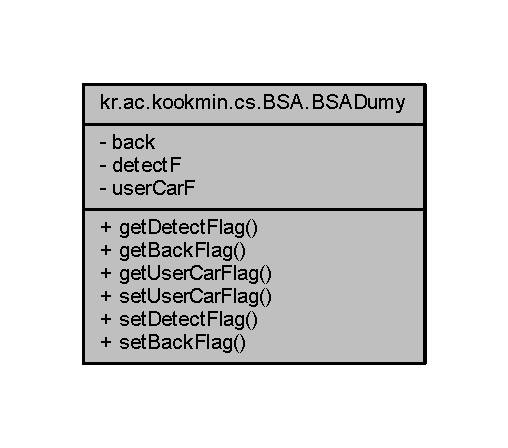
\includegraphics[width=244pt]{classkr_1_1ac_1_1kookmin_1_1cs_1_1_b_s_a_1_1_b_s_a_dumy__coll__graph}
\end{center}
\end{figure}
\subsection*{정적 Public 멤버 함수}
\begin{DoxyCompactItemize}
\item 
static boolean \hyperlink{classkr_1_1ac_1_1kookmin_1_1cs_1_1_b_s_a_1_1_b_s_a_dumy_a91ee92dabba61da78268000d16735492}{get\+Detect\+Flag} ()
\item 
static boolean \hyperlink{classkr_1_1ac_1_1kookmin_1_1cs_1_1_b_s_a_1_1_b_s_a_dumy_a636e4ba1005c1d6c31079c086529f702}{get\+Back\+Flag} ()
\item 
static boolean \hyperlink{classkr_1_1ac_1_1kookmin_1_1cs_1_1_b_s_a_1_1_b_s_a_dumy_a9adca5a9e0136713dee1023f90acc829}{get\+User\+Car\+Flag} ()
\item 
static void \hyperlink{classkr_1_1ac_1_1kookmin_1_1cs_1_1_b_s_a_1_1_b_s_a_dumy_afe0bc16e3df1ff7bcf74d310c6a0f009}{set\+User\+Car\+Flag} (boolean flag)
\item 
static void \hyperlink{classkr_1_1ac_1_1kookmin_1_1cs_1_1_b_s_a_1_1_b_s_a_dumy_ab432efb89032b15aab5d86c18129ca47}{set\+Detect\+Flag} (boolean flag)
\item 
static void \hyperlink{classkr_1_1ac_1_1kookmin_1_1cs_1_1_b_s_a_1_1_b_s_a_dumy_ab95daa3749ab4050189bbfe02064eb42}{set\+Back\+Flag} (boolean flag)
\end{DoxyCompactItemize}
\subsection*{정적 Private 속성}
\begin{DoxyCompactItemize}
\item 
static boolean \hyperlink{classkr_1_1ac_1_1kookmin_1_1cs_1_1_b_s_a_1_1_b_s_a_dumy_a83dfdbc6e79d76f3fb82f19e88526aea}{back} =false
\item 
static boolean \hyperlink{classkr_1_1ac_1_1kookmin_1_1cs_1_1_b_s_a_1_1_b_s_a_dumy_a96b15a50850eb2c92dbb11ee225ff1ef}{detect\+F} =false
\item 
static boolean \hyperlink{classkr_1_1ac_1_1kookmin_1_1cs_1_1_b_s_a_1_1_b_s_a_dumy_a2c1c5de6eb79fb484fba63ca2a9791f5}{user\+Car\+F} =false
\end{DoxyCompactItemize}


\subsection{상세한 설명}
This class , to detect the \hyperlink{namespacekr_1_1ac_1_1kookmin_1_1cs_1_1_b_s_a}{B\+S\+A} signal . 

\begin{DoxyAuthor}{작성자}
Im-\/gisung,Hong-\/sunghyeon 
\end{DoxyAuthor}


\subsection{멤버 함수 문서화}
\hypertarget{classkr_1_1ac_1_1kookmin_1_1cs_1_1_b_s_a_1_1_b_s_a_dumy_a636e4ba1005c1d6c31079c086529f702}{}\index{kr\+::ac\+::kookmin\+::cs\+::\+B\+S\+A\+::\+B\+S\+A\+Dumy@{kr\+::ac\+::kookmin\+::cs\+::\+B\+S\+A\+::\+B\+S\+A\+Dumy}!get\+Back\+Flag@{get\+Back\+Flag}}
\index{get\+Back\+Flag@{get\+Back\+Flag}!kr\+::ac\+::kookmin\+::cs\+::\+B\+S\+A\+::\+B\+S\+A\+Dumy@{kr\+::ac\+::kookmin\+::cs\+::\+B\+S\+A\+::\+B\+S\+A\+Dumy}}
\subsubsection[{get\+Back\+Flag}]{\setlength{\rightskip}{0pt plus 5cm}static boolean kr.\+ac.\+kookmin.\+cs.\+B\+S\+A.\+B\+S\+A\+Dumy.\+get\+Back\+Flag (
\begin{DoxyParamCaption}
{}
\end{DoxyParamCaption}
)\hspace{0.3cm}{\ttfamily [static]}}\label{classkr_1_1ac_1_1kookmin_1_1cs_1_1_b_s_a_1_1_b_s_a_dumy_a636e4ba1005c1d6c31079c086529f702}

\begin{DoxyCode}
28                                       \{
29     \textcolor{keywordflow}{return} \hyperlink{classkr_1_1ac_1_1kookmin_1_1cs_1_1_b_s_a_1_1_b_s_a_dumy_a83dfdbc6e79d76f3fb82f19e88526aea}{back};
30   \}
\end{DoxyCode}


이 함수를 호출하는 함수들에 대한 그래프입니다.\+:\nopagebreak
\begin{figure}[H]
\begin{center}
\leavevmode
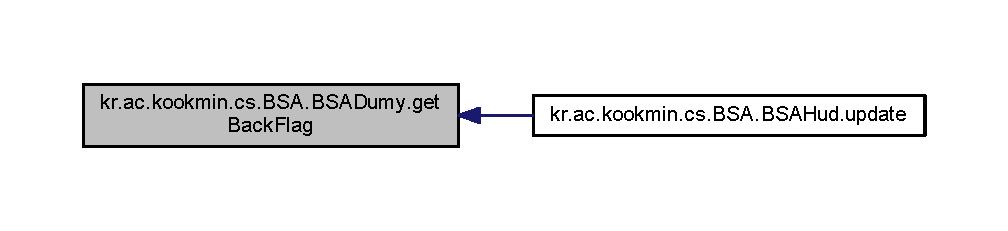
\includegraphics[width=350pt]{classkr_1_1ac_1_1kookmin_1_1cs_1_1_b_s_a_1_1_b_s_a_dumy_a636e4ba1005c1d6c31079c086529f702_icgraph}
\end{center}
\end{figure}


\hypertarget{classkr_1_1ac_1_1kookmin_1_1cs_1_1_b_s_a_1_1_b_s_a_dumy_a91ee92dabba61da78268000d16735492}{}\index{kr\+::ac\+::kookmin\+::cs\+::\+B\+S\+A\+::\+B\+S\+A\+Dumy@{kr\+::ac\+::kookmin\+::cs\+::\+B\+S\+A\+::\+B\+S\+A\+Dumy}!get\+Detect\+Flag@{get\+Detect\+Flag}}
\index{get\+Detect\+Flag@{get\+Detect\+Flag}!kr\+::ac\+::kookmin\+::cs\+::\+B\+S\+A\+::\+B\+S\+A\+Dumy@{kr\+::ac\+::kookmin\+::cs\+::\+B\+S\+A\+::\+B\+S\+A\+Dumy}}
\subsubsection[{get\+Detect\+Flag}]{\setlength{\rightskip}{0pt plus 5cm}static boolean kr.\+ac.\+kookmin.\+cs.\+B\+S\+A.\+B\+S\+A\+Dumy.\+get\+Detect\+Flag (
\begin{DoxyParamCaption}
{}
\end{DoxyParamCaption}
)\hspace{0.3cm}{\ttfamily [static]}}\label{classkr_1_1ac_1_1kookmin_1_1cs_1_1_b_s_a_1_1_b_s_a_dumy_a91ee92dabba61da78268000d16735492}

\begin{DoxyCode}
25                                         \{
26     \textcolor{keywordflow}{return} \hyperlink{classkr_1_1ac_1_1kookmin_1_1cs_1_1_b_s_a_1_1_b_s_a_dumy_a96b15a50850eb2c92dbb11ee225ff1ef}{detectF};
27   \}
\end{DoxyCode}


이 함수를 호출하는 함수들에 대한 그래프입니다.\+:\nopagebreak
\begin{figure}[H]
\begin{center}
\leavevmode
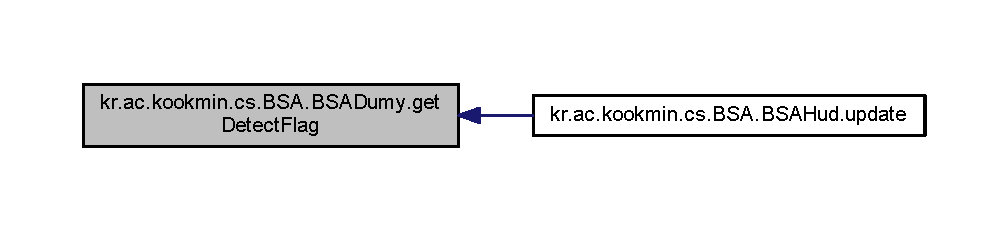
\includegraphics[width=350pt]{classkr_1_1ac_1_1kookmin_1_1cs_1_1_b_s_a_1_1_b_s_a_dumy_a91ee92dabba61da78268000d16735492_icgraph}
\end{center}
\end{figure}


\hypertarget{classkr_1_1ac_1_1kookmin_1_1cs_1_1_b_s_a_1_1_b_s_a_dumy_a9adca5a9e0136713dee1023f90acc829}{}\index{kr\+::ac\+::kookmin\+::cs\+::\+B\+S\+A\+::\+B\+S\+A\+Dumy@{kr\+::ac\+::kookmin\+::cs\+::\+B\+S\+A\+::\+B\+S\+A\+Dumy}!get\+User\+Car\+Flag@{get\+User\+Car\+Flag}}
\index{get\+User\+Car\+Flag@{get\+User\+Car\+Flag}!kr\+::ac\+::kookmin\+::cs\+::\+B\+S\+A\+::\+B\+S\+A\+Dumy@{kr\+::ac\+::kookmin\+::cs\+::\+B\+S\+A\+::\+B\+S\+A\+Dumy}}
\subsubsection[{get\+User\+Car\+Flag}]{\setlength{\rightskip}{0pt plus 5cm}static boolean kr.\+ac.\+kookmin.\+cs.\+B\+S\+A.\+B\+S\+A\+Dumy.\+get\+User\+Car\+Flag (
\begin{DoxyParamCaption}
{}
\end{DoxyParamCaption}
)\hspace{0.3cm}{\ttfamily [static]}}\label{classkr_1_1ac_1_1kookmin_1_1cs_1_1_b_s_a_1_1_b_s_a_dumy_a9adca5a9e0136713dee1023f90acc829}

\begin{DoxyCode}
31                                          \{
32     \textcolor{keywordflow}{return} \hyperlink{classkr_1_1ac_1_1kookmin_1_1cs_1_1_b_s_a_1_1_b_s_a_dumy_a2c1c5de6eb79fb484fba63ca2a9791f5}{userCarF};
33   \}
\end{DoxyCode}
\hypertarget{classkr_1_1ac_1_1kookmin_1_1cs_1_1_b_s_a_1_1_b_s_a_dumy_ab95daa3749ab4050189bbfe02064eb42}{}\index{kr\+::ac\+::kookmin\+::cs\+::\+B\+S\+A\+::\+B\+S\+A\+Dumy@{kr\+::ac\+::kookmin\+::cs\+::\+B\+S\+A\+::\+B\+S\+A\+Dumy}!set\+Back\+Flag@{set\+Back\+Flag}}
\index{set\+Back\+Flag@{set\+Back\+Flag}!kr\+::ac\+::kookmin\+::cs\+::\+B\+S\+A\+::\+B\+S\+A\+Dumy@{kr\+::ac\+::kookmin\+::cs\+::\+B\+S\+A\+::\+B\+S\+A\+Dumy}}
\subsubsection[{set\+Back\+Flag}]{\setlength{\rightskip}{0pt plus 5cm}static void kr.\+ac.\+kookmin.\+cs.\+B\+S\+A.\+B\+S\+A\+Dumy.\+set\+Back\+Flag (
\begin{DoxyParamCaption}
\item[{boolean}]{flag}
\end{DoxyParamCaption}
)\hspace{0.3cm}{\ttfamily [static]}}\label{classkr_1_1ac_1_1kookmin_1_1cs_1_1_b_s_a_1_1_b_s_a_dumy_ab95daa3749ab4050189bbfe02064eb42}

\begin{DoxyCode}
40                                                \{
41     \hyperlink{classkr_1_1ac_1_1kookmin_1_1cs_1_1_b_s_a_1_1_b_s_a_dumy_a83dfdbc6e79d76f3fb82f19e88526aea}{back} = flag;        
42   \}
\end{DoxyCode}
\hypertarget{classkr_1_1ac_1_1kookmin_1_1cs_1_1_b_s_a_1_1_b_s_a_dumy_ab432efb89032b15aab5d86c18129ca47}{}\index{kr\+::ac\+::kookmin\+::cs\+::\+B\+S\+A\+::\+B\+S\+A\+Dumy@{kr\+::ac\+::kookmin\+::cs\+::\+B\+S\+A\+::\+B\+S\+A\+Dumy}!set\+Detect\+Flag@{set\+Detect\+Flag}}
\index{set\+Detect\+Flag@{set\+Detect\+Flag}!kr\+::ac\+::kookmin\+::cs\+::\+B\+S\+A\+::\+B\+S\+A\+Dumy@{kr\+::ac\+::kookmin\+::cs\+::\+B\+S\+A\+::\+B\+S\+A\+Dumy}}
\subsubsection[{set\+Detect\+Flag}]{\setlength{\rightskip}{0pt plus 5cm}static void kr.\+ac.\+kookmin.\+cs.\+B\+S\+A.\+B\+S\+A\+Dumy.\+set\+Detect\+Flag (
\begin{DoxyParamCaption}
\item[{boolean}]{flag}
\end{DoxyParamCaption}
)\hspace{0.3cm}{\ttfamily [static]}}\label{classkr_1_1ac_1_1kookmin_1_1cs_1_1_b_s_a_1_1_b_s_a_dumy_ab432efb89032b15aab5d86c18129ca47}

\begin{DoxyCode}
37                                                  \{
38     \hyperlink{classkr_1_1ac_1_1kookmin_1_1cs_1_1_b_s_a_1_1_b_s_a_dumy_a96b15a50850eb2c92dbb11ee225ff1ef}{detectF} = flag;      
39   \}
\end{DoxyCode}
\hypertarget{classkr_1_1ac_1_1kookmin_1_1cs_1_1_b_s_a_1_1_b_s_a_dumy_afe0bc16e3df1ff7bcf74d310c6a0f009}{}\index{kr\+::ac\+::kookmin\+::cs\+::\+B\+S\+A\+::\+B\+S\+A\+Dumy@{kr\+::ac\+::kookmin\+::cs\+::\+B\+S\+A\+::\+B\+S\+A\+Dumy}!set\+User\+Car\+Flag@{set\+User\+Car\+Flag}}
\index{set\+User\+Car\+Flag@{set\+User\+Car\+Flag}!kr\+::ac\+::kookmin\+::cs\+::\+B\+S\+A\+::\+B\+S\+A\+Dumy@{kr\+::ac\+::kookmin\+::cs\+::\+B\+S\+A\+::\+B\+S\+A\+Dumy}}
\subsubsection[{set\+User\+Car\+Flag}]{\setlength{\rightskip}{0pt plus 5cm}static void kr.\+ac.\+kookmin.\+cs.\+B\+S\+A.\+B\+S\+A\+Dumy.\+set\+User\+Car\+Flag (
\begin{DoxyParamCaption}
\item[{boolean}]{flag}
\end{DoxyParamCaption}
)\hspace{0.3cm}{\ttfamily [static]}}\label{classkr_1_1ac_1_1kookmin_1_1cs_1_1_b_s_a_1_1_b_s_a_dumy_afe0bc16e3df1ff7bcf74d310c6a0f009}

\begin{DoxyCode}
34                                                   \{
35     \hyperlink{classkr_1_1ac_1_1kookmin_1_1cs_1_1_b_s_a_1_1_b_s_a_dumy_a2c1c5de6eb79fb484fba63ca2a9791f5}{userCarF} = flag;
36   \}
\end{DoxyCode}


\subsection{멤버 데이타 문서화}
\hypertarget{classkr_1_1ac_1_1kookmin_1_1cs_1_1_b_s_a_1_1_b_s_a_dumy_a83dfdbc6e79d76f3fb82f19e88526aea}{}\index{kr\+::ac\+::kookmin\+::cs\+::\+B\+S\+A\+::\+B\+S\+A\+Dumy@{kr\+::ac\+::kookmin\+::cs\+::\+B\+S\+A\+::\+B\+S\+A\+Dumy}!back@{back}}
\index{back@{back}!kr\+::ac\+::kookmin\+::cs\+::\+B\+S\+A\+::\+B\+S\+A\+Dumy@{kr\+::ac\+::kookmin\+::cs\+::\+B\+S\+A\+::\+B\+S\+A\+Dumy}}
\subsubsection[{back}]{\setlength{\rightskip}{0pt plus 5cm}boolean kr.\+ac.\+kookmin.\+cs.\+B\+S\+A.\+B\+S\+A\+Dumy.\+back =false\hspace{0.3cm}{\ttfamily [static]}, {\ttfamily [private]}}\label{classkr_1_1ac_1_1kookmin_1_1cs_1_1_b_s_a_1_1_b_s_a_dumy_a83dfdbc6e79d76f3fb82f19e88526aea}
\hypertarget{classkr_1_1ac_1_1kookmin_1_1cs_1_1_b_s_a_1_1_b_s_a_dumy_a96b15a50850eb2c92dbb11ee225ff1ef}{}\index{kr\+::ac\+::kookmin\+::cs\+::\+B\+S\+A\+::\+B\+S\+A\+Dumy@{kr\+::ac\+::kookmin\+::cs\+::\+B\+S\+A\+::\+B\+S\+A\+Dumy}!detect\+F@{detect\+F}}
\index{detect\+F@{detect\+F}!kr\+::ac\+::kookmin\+::cs\+::\+B\+S\+A\+::\+B\+S\+A\+Dumy@{kr\+::ac\+::kookmin\+::cs\+::\+B\+S\+A\+::\+B\+S\+A\+Dumy}}
\subsubsection[{detect\+F}]{\setlength{\rightskip}{0pt plus 5cm}boolean kr.\+ac.\+kookmin.\+cs.\+B\+S\+A.\+B\+S\+A\+Dumy.\+detect\+F =false\hspace{0.3cm}{\ttfamily [static]}, {\ttfamily [private]}}\label{classkr_1_1ac_1_1kookmin_1_1cs_1_1_b_s_a_1_1_b_s_a_dumy_a96b15a50850eb2c92dbb11ee225ff1ef}
\hypertarget{classkr_1_1ac_1_1kookmin_1_1cs_1_1_b_s_a_1_1_b_s_a_dumy_a2c1c5de6eb79fb484fba63ca2a9791f5}{}\index{kr\+::ac\+::kookmin\+::cs\+::\+B\+S\+A\+::\+B\+S\+A\+Dumy@{kr\+::ac\+::kookmin\+::cs\+::\+B\+S\+A\+::\+B\+S\+A\+Dumy}!user\+Car\+F@{user\+Car\+F}}
\index{user\+Car\+F@{user\+Car\+F}!kr\+::ac\+::kookmin\+::cs\+::\+B\+S\+A\+::\+B\+S\+A\+Dumy@{kr\+::ac\+::kookmin\+::cs\+::\+B\+S\+A\+::\+B\+S\+A\+Dumy}}
\subsubsection[{user\+Car\+F}]{\setlength{\rightskip}{0pt plus 5cm}boolean kr.\+ac.\+kookmin.\+cs.\+B\+S\+A.\+B\+S\+A\+Dumy.\+user\+Car\+F =false\hspace{0.3cm}{\ttfamily [static]}, {\ttfamily [private]}}\label{classkr_1_1ac_1_1kookmin_1_1cs_1_1_b_s_a_1_1_b_s_a_dumy_a2c1c5de6eb79fb484fba63ca2a9791f5}


이 클래스에 대한 문서화 페이지는 다음의 파일로부터 생성되었습니다.\+:\begin{DoxyCompactItemize}
\item 
C\+:/\+Users/\+Karasion/git/\+Capstone2015-\/\+Purple\+Ocean/src/kr/ac/kookmin/cs/\+B\+S\+A/\hyperlink{_b_s_a_dumy_8java}{B\+S\+A\+Dumy.\+java}\end{DoxyCompactItemize}

\hypertarget{classkr_1_1ac_1_1kookmin_1_1cs_1_1_b_s_a_1_1_b_s_a_hud}{}\section{kr.\+ac.\+kookmin.\+cs.\+B\+S\+A.\+B\+S\+A\+Hud 클래스 참조}
\label{classkr_1_1ac_1_1kookmin_1_1cs_1_1_b_s_a_1_1_b_s_a_hud}\index{kr.\+ac.\+kookmin.\+cs.\+B\+S\+A.\+B\+S\+A\+Hud@{kr.\+ac.\+kookmin.\+cs.\+B\+S\+A.\+B\+S\+A\+Hud}}


This class serves to output information related to the \hyperlink{namespacekr_1_1ac_1_1kookmin_1_1cs_1_1_b_s_a}{B\+S\+A} to Hud.  




kr.\+ac.\+kookmin.\+cs.\+B\+S\+A.\+B\+S\+A\+Hud에 대한 상속 다이어그램 \+: \nopagebreak
\begin{figure}[H]
\begin{center}
\leavevmode
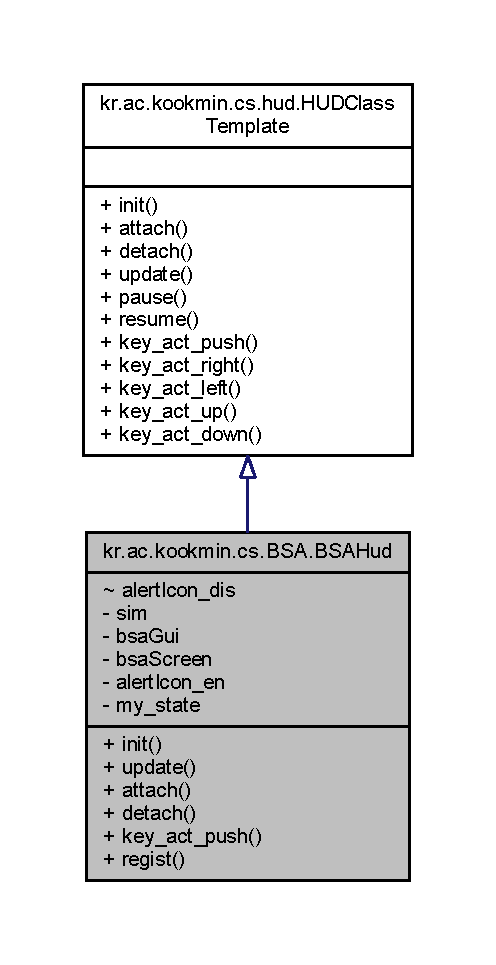
\includegraphics[width=238pt]{classkr_1_1ac_1_1kookmin_1_1cs_1_1_b_s_a_1_1_b_s_a_hud__inherit__graph}
\end{center}
\end{figure}


kr.\+ac.\+kookmin.\+cs.\+B\+S\+A.\+B\+S\+A\+Hud에 대한 협력 다이어그램\+:\nopagebreak
\begin{figure}[H]
\begin{center}
\leavevmode
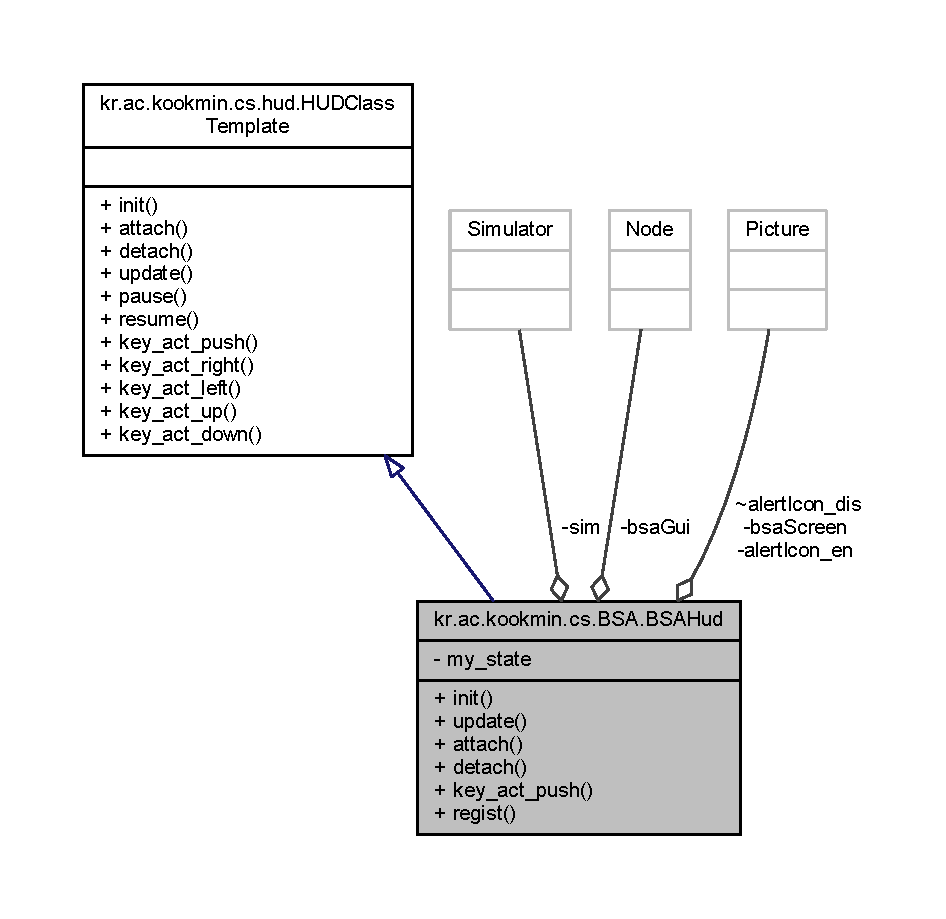
\includegraphics[width=350pt]{classkr_1_1ac_1_1kookmin_1_1cs_1_1_b_s_a_1_1_b_s_a_hud__coll__graph}
\end{center}
\end{figure}
\subsection*{Public 멤버 함수}
\begin{DoxyCompactItemize}
\item 
void \hyperlink{classkr_1_1ac_1_1kookmin_1_1cs_1_1_b_s_a_1_1_b_s_a_hud_a98a07afc224f8f9374e934cb69f1de00}{init} (Simulator simulator)
\begin{DoxyCompactList}\small\item\em It is a method of initializing the related elements to \hyperlink{namespacekr_1_1ac_1_1kookmin_1_1cs_1_1_b_s_a}{B\+S\+A}. \end{DoxyCompactList}\item 
void \hyperlink{classkr_1_1ac_1_1kookmin_1_1cs_1_1_b_s_a_1_1_b_s_a_hud_a74c1637acb3398ef86da500f100c630d}{update} ()
\begin{DoxyCompactList}\small\item\em Is a method to be executed in real time on the simulator . \end{DoxyCompactList}\item 
void \hyperlink{classkr_1_1ac_1_1kookmin_1_1cs_1_1_b_s_a_1_1_b_s_a_hud_aa92574e989e21ef14b0c53f0220dc488}{attach} ()
\begin{DoxyCompactList}\small\item\em This method , attach the node associated with the \hyperlink{namespacekr_1_1ac_1_1kookmin_1_1cs_1_1_b_s_a}{B\+S\+A} to simulator. \end{DoxyCompactList}\item 
void \hyperlink{classkr_1_1ac_1_1kookmin_1_1cs_1_1_b_s_a_1_1_b_s_a_hud_a7f2ad3023b835013511046876de1b38b}{detach} ()
\begin{DoxyCompactList}\small\item\em This method , detach the node associated with the \hyperlink{namespacekr_1_1ac_1_1kookmin_1_1cs_1_1_b_s_a}{B\+S\+A} to simulator. \end{DoxyCompactList}\item 
void \hyperlink{classkr_1_1ac_1_1kookmin_1_1cs_1_1_b_s_a_1_1_b_s_a_hud_a3e66906fe591f6d39d6305ff17444464}{key\+\_\+act\+\_\+push} ()
\begin{DoxyCompactList}\small\item\em When you press the push button in the G-\/\+H\+U\+B, it is a method to be executed . \end{DoxyCompactList}\end{DoxyCompactItemize}
\subsection*{정적 Public 멤버 함수}
\begin{DoxyCompactItemize}
\item 
static void \hyperlink{classkr_1_1ac_1_1kookmin_1_1cs_1_1_b_s_a_1_1_b_s_a_hud_a61e5431be2f589f6d4d32cf70efbe880}{regist} ()
\begin{DoxyCompactList}\small\item\em This method to register an instance of class \hyperlink{namespacekr_1_1ac_1_1kookmin_1_1cs_1_1_b_s_a}{B\+S\+A} to H\+U\+D\+Management. \end{DoxyCompactList}\end{DoxyCompactItemize}
\subsection*{정적 Private 속성}
\begin{DoxyCompactItemize}
\item 
static Simulator \hyperlink{classkr_1_1ac_1_1kookmin_1_1cs_1_1_b_s_a_1_1_b_s_a_hud_a94269498fba32b6567a641dc5fa3f3be}{sim}
\item 
static Node \hyperlink{classkr_1_1ac_1_1kookmin_1_1cs_1_1_b_s_a_1_1_b_s_a_hud_a2401197078adb71369a9bc30d66ee9f0}{bsa\+Gui}
\item 
static Picture \hyperlink{classkr_1_1ac_1_1kookmin_1_1cs_1_1_b_s_a_1_1_b_s_a_hud_a634791106770e96193088681b4a7cf06}{bsa\+Screen}
\item 
static Picture \hyperlink{classkr_1_1ac_1_1kookmin_1_1cs_1_1_b_s_a_1_1_b_s_a_hud_a4bacb44beb3117557129c5e340ead0c4}{alert\+Icon\+\_\+en}
\item 
static int \hyperlink{classkr_1_1ac_1_1kookmin_1_1cs_1_1_b_s_a_1_1_b_s_a_hud_a90a752df5176c831c74f36190f77c0a2}{my\+\_\+state}
\end{DoxyCompactItemize}


\subsection{상세한 설명}
This class serves to output information related to the \hyperlink{namespacekr_1_1ac_1_1kookmin_1_1cs_1_1_b_s_a}{B\+S\+A} to Hud. 

In the simulator , If the user selects the \hyperlink{namespacekr_1_1ac_1_1kookmin_1_1cs_1_1_b_s_a}{B\+S\+A} function , if the car has been detected around the user , print to information related to the \hyperlink{namespacekr_1_1ac_1_1kookmin_1_1cs_1_1_b_s_a}{B\+S\+A} to the appropriate position of H\+U\+D. \begin{DoxyAuthor}{작성자}
Im-\/gisung,Jo-\/kwanghyeon 
\end{DoxyAuthor}


\subsection{멤버 함수 문서화}
\hypertarget{classkr_1_1ac_1_1kookmin_1_1cs_1_1_b_s_a_1_1_b_s_a_hud_aa92574e989e21ef14b0c53f0220dc488}{}\index{kr\+::ac\+::kookmin\+::cs\+::\+B\+S\+A\+::\+B\+S\+A\+Hud@{kr\+::ac\+::kookmin\+::cs\+::\+B\+S\+A\+::\+B\+S\+A\+Hud}!attach@{attach}}
\index{attach@{attach}!kr\+::ac\+::kookmin\+::cs\+::\+B\+S\+A\+::\+B\+S\+A\+Hud@{kr\+::ac\+::kookmin\+::cs\+::\+B\+S\+A\+::\+B\+S\+A\+Hud}}
\subsubsection[{attach}]{\setlength{\rightskip}{0pt plus 5cm}void kr.\+ac.\+kookmin.\+cs.\+B\+S\+A.\+B\+S\+A\+Hud.\+attach (
\begin{DoxyParamCaption}
{}
\end{DoxyParamCaption}
)}\label{classkr_1_1ac_1_1kookmin_1_1cs_1_1_b_s_a_1_1_b_s_a_hud_aa92574e989e21ef14b0c53f0220dc488}


This method , attach the node associated with the \hyperlink{namespacekr_1_1ac_1_1kookmin_1_1cs_1_1_b_s_a}{B\+S\+A} to simulator. 


\begin{DoxyParams}{매개변수}
{\em nothing} & \\
\hline
\end{DoxyParams}
\begin{DoxyReturn}{반환값}
nothing 
\end{DoxyReturn}

\begin{DoxyCode}
104                        \{
105     HUDManagement.attach(\hyperlink{classkr_1_1ac_1_1kookmin_1_1cs_1_1_b_s_a_1_1_b_s_a_hud_a2401197078adb71369a9bc30d66ee9f0}{bsaGui});
106   \}
\end{DoxyCode}


이 함수 내부에서 호출하는 함수들에 대한 그래프입니다.\+:\nopagebreak
\begin{figure}[H]
\begin{center}
\leavevmode
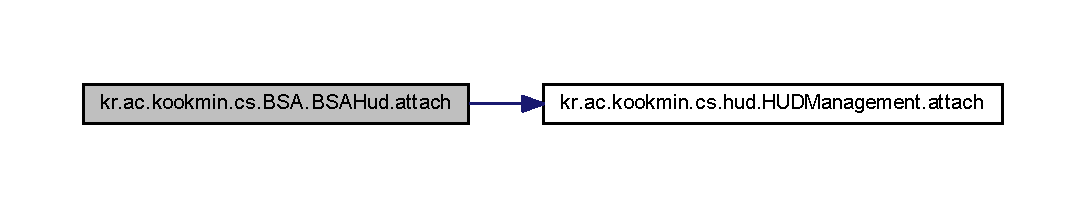
\includegraphics[width=350pt]{classkr_1_1ac_1_1kookmin_1_1cs_1_1_b_s_a_1_1_b_s_a_hud_aa92574e989e21ef14b0c53f0220dc488_cgraph}
\end{center}
\end{figure}




이 함수를 호출하는 함수들에 대한 그래프입니다.\+:\nopagebreak
\begin{figure}[H]
\begin{center}
\leavevmode
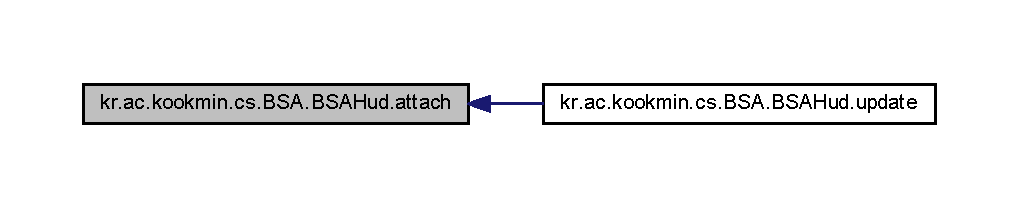
\includegraphics[width=350pt]{classkr_1_1ac_1_1kookmin_1_1cs_1_1_b_s_a_1_1_b_s_a_hud_aa92574e989e21ef14b0c53f0220dc488_icgraph}
\end{center}
\end{figure}


\hypertarget{classkr_1_1ac_1_1kookmin_1_1cs_1_1_b_s_a_1_1_b_s_a_hud_a7f2ad3023b835013511046876de1b38b}{}\index{kr\+::ac\+::kookmin\+::cs\+::\+B\+S\+A\+::\+B\+S\+A\+Hud@{kr\+::ac\+::kookmin\+::cs\+::\+B\+S\+A\+::\+B\+S\+A\+Hud}!detach@{detach}}
\index{detach@{detach}!kr\+::ac\+::kookmin\+::cs\+::\+B\+S\+A\+::\+B\+S\+A\+Hud@{kr\+::ac\+::kookmin\+::cs\+::\+B\+S\+A\+::\+B\+S\+A\+Hud}}
\subsubsection[{detach}]{\setlength{\rightskip}{0pt plus 5cm}void kr.\+ac.\+kookmin.\+cs.\+B\+S\+A.\+B\+S\+A\+Hud.\+detach (
\begin{DoxyParamCaption}
{}
\end{DoxyParamCaption}
)}\label{classkr_1_1ac_1_1kookmin_1_1cs_1_1_b_s_a_1_1_b_s_a_hud_a7f2ad3023b835013511046876de1b38b}


This method , detach the node associated with the \hyperlink{namespacekr_1_1ac_1_1kookmin_1_1cs_1_1_b_s_a}{B\+S\+A} to simulator. 


\begin{DoxyParams}{매개변수}
{\em nothing} & \\
\hline
\end{DoxyParams}
\begin{DoxyReturn}{반환값}
nothing 
\end{DoxyReturn}

\begin{DoxyCode}
113                        \{
114     HUDManagement.detach(\hyperlink{classkr_1_1ac_1_1kookmin_1_1cs_1_1_b_s_a_1_1_b_s_a_hud_a2401197078adb71369a9bc30d66ee9f0}{bsaGui});
115   \}
\end{DoxyCode}


이 함수 내부에서 호출하는 함수들에 대한 그래프입니다.\+:\nopagebreak
\begin{figure}[H]
\begin{center}
\leavevmode
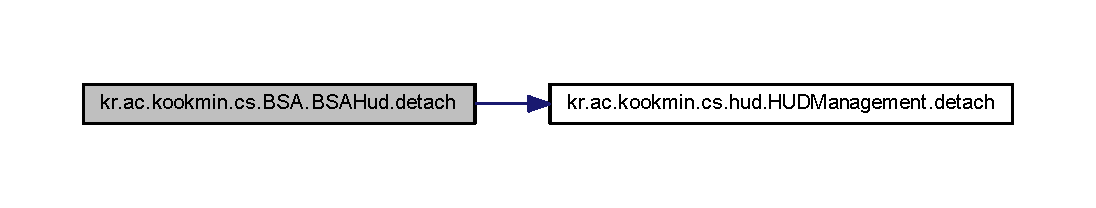
\includegraphics[width=350pt]{classkr_1_1ac_1_1kookmin_1_1cs_1_1_b_s_a_1_1_b_s_a_hud_a7f2ad3023b835013511046876de1b38b_cgraph}
\end{center}
\end{figure}




이 함수를 호출하는 함수들에 대한 그래프입니다.\+:\nopagebreak
\begin{figure}[H]
\begin{center}
\leavevmode
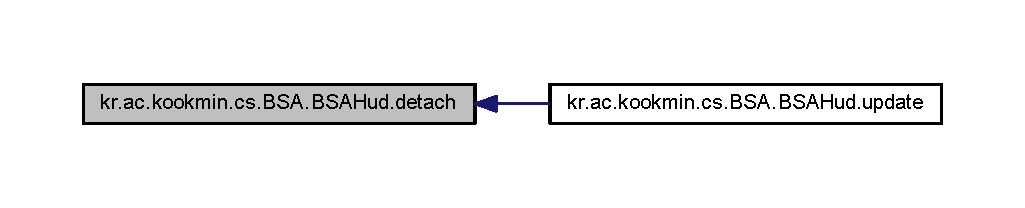
\includegraphics[width=350pt]{classkr_1_1ac_1_1kookmin_1_1cs_1_1_b_s_a_1_1_b_s_a_hud_a7f2ad3023b835013511046876de1b38b_icgraph}
\end{center}
\end{figure}


\hypertarget{classkr_1_1ac_1_1kookmin_1_1cs_1_1_b_s_a_1_1_b_s_a_hud_a98a07afc224f8f9374e934cb69f1de00}{}\index{kr\+::ac\+::kookmin\+::cs\+::\+B\+S\+A\+::\+B\+S\+A\+Hud@{kr\+::ac\+::kookmin\+::cs\+::\+B\+S\+A\+::\+B\+S\+A\+Hud}!init@{init}}
\index{init@{init}!kr\+::ac\+::kookmin\+::cs\+::\+B\+S\+A\+::\+B\+S\+A\+Hud@{kr\+::ac\+::kookmin\+::cs\+::\+B\+S\+A\+::\+B\+S\+A\+Hud}}
\subsubsection[{init}]{\setlength{\rightskip}{0pt plus 5cm}void kr.\+ac.\+kookmin.\+cs.\+B\+S\+A.\+B\+S\+A\+Hud.\+init (
\begin{DoxyParamCaption}
\item[{Simulator}]{simulator}
\end{DoxyParamCaption}
)}\label{classkr_1_1ac_1_1kookmin_1_1cs_1_1_b_s_a_1_1_b_s_a_hud_a98a07afc224f8f9374e934cb69f1de00}


It is a method of initializing the related elements to \hyperlink{namespacekr_1_1ac_1_1kookmin_1_1cs_1_1_b_s_a}{B\+S\+A}. 

register the associated element to \hyperlink{namespacekr_1_1ac_1_1kookmin_1_1cs_1_1_b_s_a}{B\+S\+A} icon elements and \hyperlink{namespacekr_1_1ac_1_1kookmin_1_1cs_1_1_b_s_a}{B\+S\+A} content in the simulator object 
\begin{DoxyParams}{매개변수}
{\em simulator} & a Simulator object \\
\hline
\end{DoxyParams}
\begin{DoxyReturn}{반환값}
nothing 
\end{DoxyReturn}

\begin{DoxyCode}
47   \{
48     \hyperlink{classkr_1_1ac_1_1kookmin_1_1cs_1_1_b_s_a_1_1_b_s_a_hud_a94269498fba32b6567a641dc5fa3f3be}{sim} = simulator;
49     \hyperlink{classkr_1_1ac_1_1kookmin_1_1cs_1_1_b_s_a_1_1_b_s_a_hud_a2401197078adb71369a9bc30d66ee9f0}{bsaGui}=\textcolor{keyword}{new} Node(\textcolor{stringliteral}{"BSAGui"});
50 
51     \hyperlink{classkr_1_1ac_1_1kookmin_1_1cs_1_1_b_s_a_1_1_b_s_a_hud_a634791106770e96193088681b4a7cf06}{bsaScreen} = \textcolor{keyword}{new} Picture(\textcolor{stringliteral}{"bsaScreen"});
52     \hyperlink{classkr_1_1ac_1_1kookmin_1_1cs_1_1_b_s_a_1_1_b_s_a_hud_a634791106770e96193088681b4a7cf06}{bsaScreen}.setImage(\hyperlink{classkr_1_1ac_1_1kookmin_1_1cs_1_1_b_s_a_1_1_b_s_a_hud_a94269498fba32b6567a641dc5fa3f3be}{sim}.getAssetManager(), \textcolor{stringliteral}{"Textures/icons/alert/alert\_safe.png"}, \textcolor{keyword}{true});
53     \hyperlink{classkr_1_1ac_1_1kookmin_1_1cs_1_1_b_s_a_1_1_b_s_a_hud_a634791106770e96193088681b4a7cf06}{bsaScreen}.setWidth(231);
54     \hyperlink{classkr_1_1ac_1_1kookmin_1_1cs_1_1_b_s_a_1_1_b_s_a_hud_a634791106770e96193088681b4a7cf06}{bsaScreen}.setHeight(219);
55     \hyperlink{classkr_1_1ac_1_1kookmin_1_1cs_1_1_b_s_a_1_1_b_s_a_hud_a634791106770e96193088681b4a7cf06}{bsaScreen}.setPosition(900,140);
56 
57     \hyperlink{classkr_1_1ac_1_1kookmin_1_1cs_1_1_b_s_a_1_1_b_s_a_hud_a4bacb44beb3117557129c5e340ead0c4}{alertIcon\_en} = \textcolor{keyword}{new} Picture(\textcolor{stringliteral}{"alertIcon"});
58     \hyperlink{classkr_1_1ac_1_1kookmin_1_1cs_1_1_b_s_a_1_1_b_s_a_hud_a4bacb44beb3117557129c5e340ead0c4}{alertIcon\_en}.setImage(\hyperlink{classkr_1_1ac_1_1kookmin_1_1cs_1_1_b_s_a_1_1_b_s_a_hud_a94269498fba32b6567a641dc5fa3f3be}{sim}.getAssetManager(), \textcolor{stringliteral}{"Textures/icons/menubar/menubar\_alert.png"},\textcolor{keyword}{
      true});
59     \hyperlink{classkr_1_1ac_1_1kookmin_1_1cs_1_1_b_s_a_1_1_b_s_a_hud_a4bacb44beb3117557129c5e340ead0c4}{alertIcon\_en}.setWidth(80);
60     \hyperlink{classkr_1_1ac_1_1kookmin_1_1cs_1_1_b_s_a_1_1_b_s_a_hud_a4bacb44beb3117557129c5e340ead0c4}{alertIcon\_en}.setHeight(80);
61 
62     alertIcon\_dis = \textcolor{keyword}{new} Picture(\textcolor{stringliteral}{"alertIcon"});
63     alertIcon\_dis.setImage(\hyperlink{classkr_1_1ac_1_1kookmin_1_1cs_1_1_b_s_a_1_1_b_s_a_hud_a94269498fba32b6567a641dc5fa3f3be}{sim}.getAssetManager(), \textcolor{stringliteral}{"Textures/icons/menubar/menubar\_alert\_c.png"},\textcolor{keyword}{true});
64     alertIcon\_dis.setWidth(80);
65     alertIcon\_dis.setHeight(80);
66 
67     HUDManagement.setMenuIcon(\hyperlink{classkr_1_1ac_1_1kookmin_1_1cs_1_1_b_s_a_1_1_b_s_a_hud_a4bacb44beb3117557129c5e340ead0c4}{alertIcon\_en}, alertIcon\_dis, \hyperlink{classkr_1_1ac_1_1kookmin_1_1cs_1_1_b_s_a_1_1_b_s_a_hud_a90a752df5176c831c74f36190f77c0a2}{my\_state});
68 
69     \hyperlink{classkr_1_1ac_1_1kookmin_1_1cs_1_1_b_s_a_1_1_b_s_a_hud_a2401197078adb71369a9bc30d66ee9f0}{bsaGui}.attachChild(\hyperlink{classkr_1_1ac_1_1kookmin_1_1cs_1_1_b_s_a_1_1_b_s_a_hud_a634791106770e96193088681b4a7cf06}{bsaScreen});
70   \}
\end{DoxyCode}


이 함수 내부에서 호출하는 함수들에 대한 그래프입니다.\+:\nopagebreak
\begin{figure}[H]
\begin{center}
\leavevmode
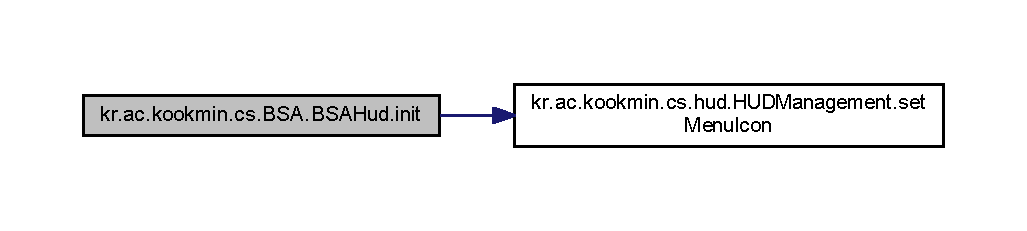
\includegraphics[width=350pt]{classkr_1_1ac_1_1kookmin_1_1cs_1_1_b_s_a_1_1_b_s_a_hud_a98a07afc224f8f9374e934cb69f1de00_cgraph}
\end{center}
\end{figure}


\hypertarget{classkr_1_1ac_1_1kookmin_1_1cs_1_1_b_s_a_1_1_b_s_a_hud_a3e66906fe591f6d39d6305ff17444464}{}\index{kr\+::ac\+::kookmin\+::cs\+::\+B\+S\+A\+::\+B\+S\+A\+Hud@{kr\+::ac\+::kookmin\+::cs\+::\+B\+S\+A\+::\+B\+S\+A\+Hud}!key\+\_\+act\+\_\+push@{key\+\_\+act\+\_\+push}}
\index{key\+\_\+act\+\_\+push@{key\+\_\+act\+\_\+push}!kr\+::ac\+::kookmin\+::cs\+::\+B\+S\+A\+::\+B\+S\+A\+Hud@{kr\+::ac\+::kookmin\+::cs\+::\+B\+S\+A\+::\+B\+S\+A\+Hud}}
\subsubsection[{key\+\_\+act\+\_\+push}]{\setlength{\rightskip}{0pt plus 5cm}void kr.\+ac.\+kookmin.\+cs.\+B\+S\+A.\+B\+S\+A\+Hud.\+key\+\_\+act\+\_\+push (
\begin{DoxyParamCaption}
{}
\end{DoxyParamCaption}
)}\label{classkr_1_1ac_1_1kookmin_1_1cs_1_1_b_s_a_1_1_b_s_a_hud_a3e66906fe591f6d39d6305ff17444464}


When you press the push button in the G-\/\+H\+U\+B, it is a method to be executed . 

menu of \hyperlink{namespacekr_1_1ac_1_1kookmin_1_1cs_1_1_b_s_a}{B\+S\+A} is selected . 
\begin{DoxyParams}{매개변수}
{\em nothing} & \\
\hline
\end{DoxyParams}
\begin{DoxyReturn}{반환값}
nothing 
\end{DoxyReturn}

\begin{DoxyCode}
124   \{
125     HUDManagement.escapeMenu();
126   \}
\end{DoxyCode}


이 함수 내부에서 호출하는 함수들에 대한 그래프입니다.\+:\nopagebreak
\begin{figure}[H]
\begin{center}
\leavevmode
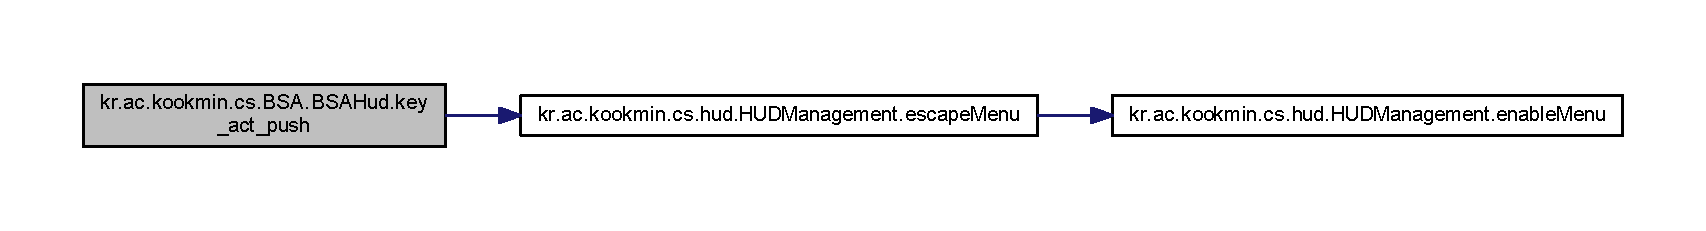
\includegraphics[width=350pt]{classkr_1_1ac_1_1kookmin_1_1cs_1_1_b_s_a_1_1_b_s_a_hud_a3e66906fe591f6d39d6305ff17444464_cgraph}
\end{center}
\end{figure}


\hypertarget{classkr_1_1ac_1_1kookmin_1_1cs_1_1_b_s_a_1_1_b_s_a_hud_a61e5431be2f589f6d4d32cf70efbe880}{}\index{kr\+::ac\+::kookmin\+::cs\+::\+B\+S\+A\+::\+B\+S\+A\+Hud@{kr\+::ac\+::kookmin\+::cs\+::\+B\+S\+A\+::\+B\+S\+A\+Hud}!regist@{regist}}
\index{regist@{regist}!kr\+::ac\+::kookmin\+::cs\+::\+B\+S\+A\+::\+B\+S\+A\+Hud@{kr\+::ac\+::kookmin\+::cs\+::\+B\+S\+A\+::\+B\+S\+A\+Hud}}
\subsubsection[{regist}]{\setlength{\rightskip}{0pt plus 5cm}static void kr.\+ac.\+kookmin.\+cs.\+B\+S\+A.\+B\+S\+A\+Hud.\+regist (
\begin{DoxyParamCaption}
{}
\end{DoxyParamCaption}
)\hspace{0.3cm}{\ttfamily [static]}}\label{classkr_1_1ac_1_1kookmin_1_1cs_1_1_b_s_a_1_1_b_s_a_hud_a61e5431be2f589f6d4d32cf70efbe880}


This method to register an instance of class \hyperlink{namespacekr_1_1ac_1_1kookmin_1_1cs_1_1_b_s_a}{B\+S\+A} to H\+U\+D\+Management. 


\begin{DoxyParams}{매개변수}
{\em nothing} & \\
\hline
\end{DoxyParams}
\begin{DoxyReturn}{반환값}
nothing 
\end{DoxyReturn}

\begin{DoxyCode}
134                               \{
135     BSAHud bsa = \textcolor{keyword}{new} BSAHud();
136     \hyperlink{classkr_1_1ac_1_1kookmin_1_1cs_1_1_b_s_a_1_1_b_s_a_hud_a90a752df5176c831c74f36190f77c0a2}{my\_state} = HUDManagement.regist(bsa);
137   \}
\end{DoxyCode}


이 함수 내부에서 호출하는 함수들에 대한 그래프입니다.\+:\nopagebreak
\begin{figure}[H]
\begin{center}
\leavevmode
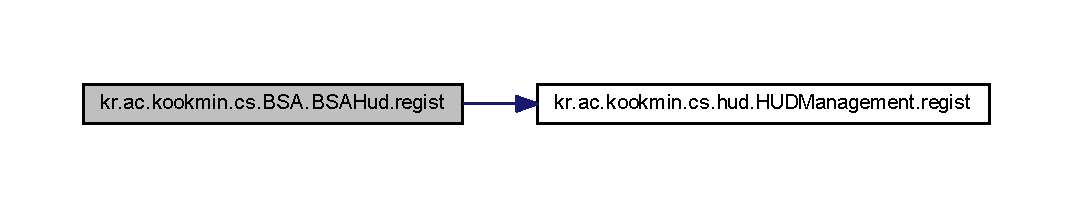
\includegraphics[width=350pt]{classkr_1_1ac_1_1kookmin_1_1cs_1_1_b_s_a_1_1_b_s_a_hud_a61e5431be2f589f6d4d32cf70efbe880_cgraph}
\end{center}
\end{figure}




이 함수를 호출하는 함수들에 대한 그래프입니다.\+:\nopagebreak
\begin{figure}[H]
\begin{center}
\leavevmode
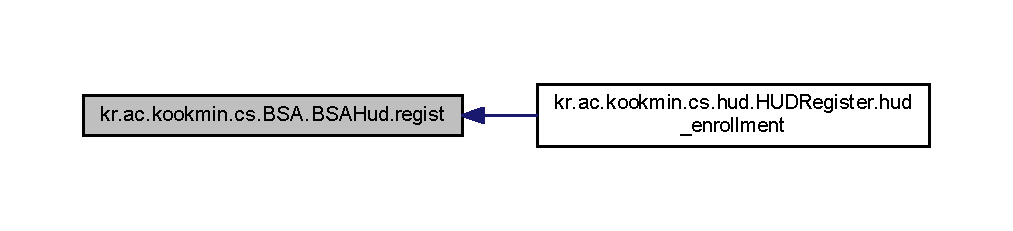
\includegraphics[width=350pt]{classkr_1_1ac_1_1kookmin_1_1cs_1_1_b_s_a_1_1_b_s_a_hud_a61e5431be2f589f6d4d32cf70efbe880_icgraph}
\end{center}
\end{figure}


\hypertarget{classkr_1_1ac_1_1kookmin_1_1cs_1_1_b_s_a_1_1_b_s_a_hud_a74c1637acb3398ef86da500f100c630d}{}\index{kr\+::ac\+::kookmin\+::cs\+::\+B\+S\+A\+::\+B\+S\+A\+Hud@{kr\+::ac\+::kookmin\+::cs\+::\+B\+S\+A\+::\+B\+S\+A\+Hud}!update@{update}}
\index{update@{update}!kr\+::ac\+::kookmin\+::cs\+::\+B\+S\+A\+::\+B\+S\+A\+Hud@{kr\+::ac\+::kookmin\+::cs\+::\+B\+S\+A\+::\+B\+S\+A\+Hud}}
\subsubsection[{update}]{\setlength{\rightskip}{0pt plus 5cm}void kr.\+ac.\+kookmin.\+cs.\+B\+S\+A.\+B\+S\+A\+Hud.\+update (
\begin{DoxyParamCaption}
{}
\end{DoxyParamCaption}
)}\label{classkr_1_1ac_1_1kookmin_1_1cs_1_1_b_s_a_1_1_b_s_a_hud_a74c1637acb3398ef86da500f100c630d}


Is a method to be executed in real time on the simulator . 

If the value of the \hyperlink{namespacekr_1_1ac_1_1kookmin_1_1cs_1_1_b_s_a}{B\+S\+A} sensor is detected , it will update the \hyperlink{namespacekr_1_1ac_1_1kookmin_1_1cs_1_1_b_s_a}{B\+S\+A} image . 
\begin{DoxyParams}{매개변수}
{\em nothing} & \\
\hline
\end{DoxyParams}
\begin{DoxyReturn}{반환값}
nothing 
\end{DoxyReturn}

\begin{DoxyCode}
79   \{
80     \textcolor{keywordflow}{if}(HUDManagement.getKeyFlag()) \{      
81       \textcolor{keywordflow}{if}(BSADumy.getDetectFlag()) \{
82         \hyperlink{classkr_1_1ac_1_1kookmin_1_1cs_1_1_b_s_a_1_1_b_s_a_hud_aa92574e989e21ef14b0c53f0220dc488}{attach}();
83         \textcolor{keywordflow}{if}(BSADumy.getBackFlag())
84           \hyperlink{classkr_1_1ac_1_1kookmin_1_1cs_1_1_b_s_a_1_1_b_s_a_hud_a634791106770e96193088681b4a7cf06}{bsaScreen}.setImage(\hyperlink{classkr_1_1ac_1_1kookmin_1_1cs_1_1_b_s_a_1_1_b_s_a_hud_a94269498fba32b6567a641dc5fa3f3be}{sim}.getAssetManager(), \textcolor{stringliteral}{"Textures/icons/alert/alert\_backside.png"}, \textcolor{keyword}{
      true});
85         \textcolor{keywordflow}{else}
86           \hyperlink{classkr_1_1ac_1_1kookmin_1_1cs_1_1_b_s_a_1_1_b_s_a_hud_a634791106770e96193088681b4a7cf06}{bsaScreen}.setImage(\hyperlink{classkr_1_1ac_1_1kookmin_1_1cs_1_1_b_s_a_1_1_b_s_a_hud_a94269498fba32b6567a641dc5fa3f3be}{sim}.getAssetManager(), \textcolor{stringliteral}{"Textures/icons/alert/alert\_rightside.png"},
       \textcolor{keyword}{true});
87       \}
88       \textcolor{keywordflow}{else}\{
89         \hyperlink{classkr_1_1ac_1_1kookmin_1_1cs_1_1_b_s_a_1_1_b_s_a_hud_a634791106770e96193088681b4a7cf06}{bsaScreen}.setImage(\hyperlink{classkr_1_1ac_1_1kookmin_1_1cs_1_1_b_s_a_1_1_b_s_a_hud_a94269498fba32b6567a641dc5fa3f3be}{sim}.getAssetManager(), \textcolor{stringliteral}{"Textures/icons/alert/alert\_safe.png"}, \textcolor{keyword}{true});
90         \textcolor{keywordflow}{if}(HUDManagement.getState() != \hyperlink{classkr_1_1ac_1_1kookmin_1_1cs_1_1_b_s_a_1_1_b_s_a_hud_a90a752df5176c831c74f36190f77c0a2}{my\_state})
91           \hyperlink{classkr_1_1ac_1_1kookmin_1_1cs_1_1_b_s_a_1_1_b_s_a_hud_a7f2ad3023b835013511046876de1b38b}{detach}();
92       \}
93 
94       \textcolor{keywordflow}{if}(HUDManagement.getState() == \hyperlink{classkr_1_1ac_1_1kookmin_1_1cs_1_1_b_s_a_1_1_b_s_a_hud_a90a752df5176c831c74f36190f77c0a2}{my\_state})
95         \hyperlink{classkr_1_1ac_1_1kookmin_1_1cs_1_1_b_s_a_1_1_b_s_a_hud_aa92574e989e21ef14b0c53f0220dc488}{attach}();
96     \}
97   \}
\end{DoxyCode}


이 함수 내부에서 호출하는 함수들에 대한 그래프입니다.\+:\nopagebreak
\begin{figure}[H]
\begin{center}
\leavevmode
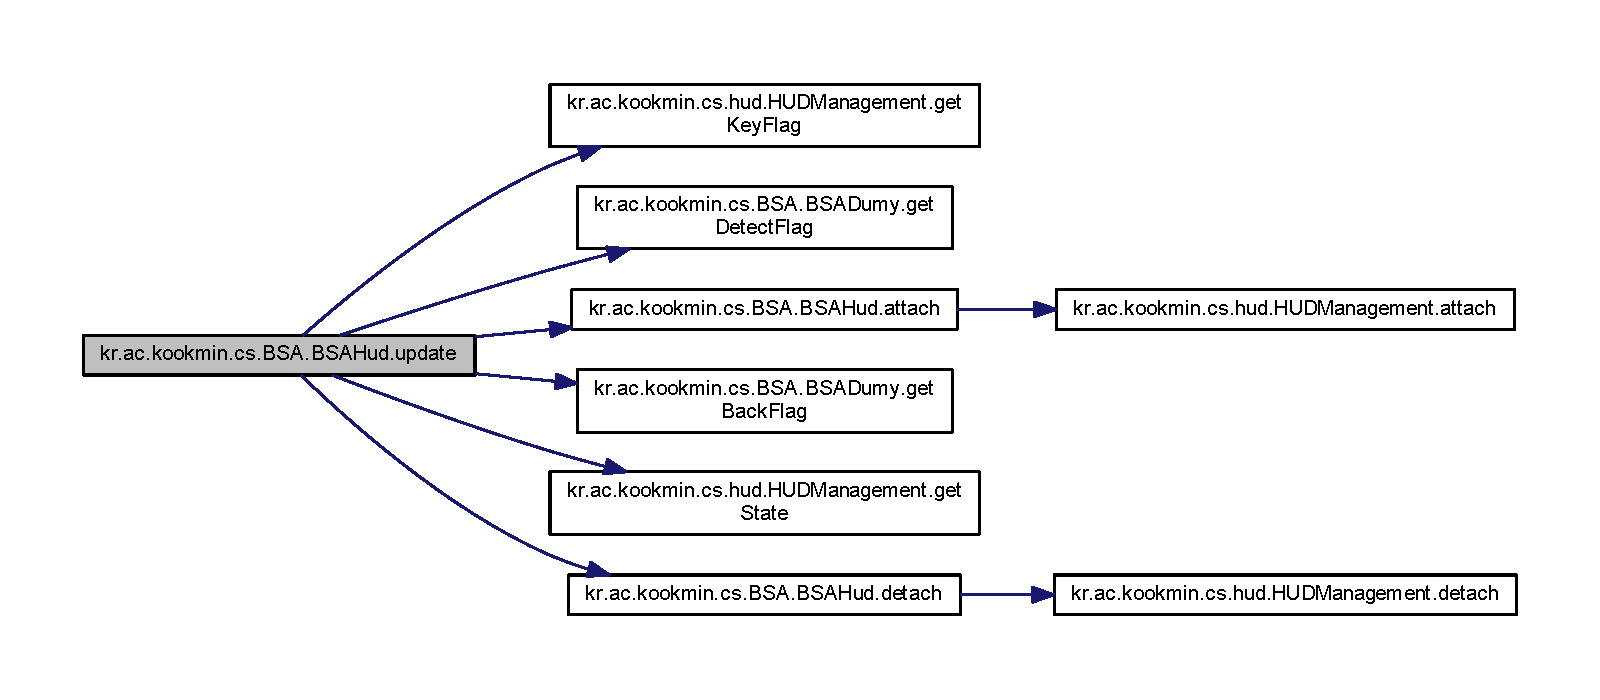
\includegraphics[width=350pt]{classkr_1_1ac_1_1kookmin_1_1cs_1_1_b_s_a_1_1_b_s_a_hud_a74c1637acb3398ef86da500f100c630d_cgraph}
\end{center}
\end{figure}




\subsection{멤버 데이타 문서화}
\hypertarget{classkr_1_1ac_1_1kookmin_1_1cs_1_1_b_s_a_1_1_b_s_a_hud_a4bacb44beb3117557129c5e340ead0c4}{}\index{kr\+::ac\+::kookmin\+::cs\+::\+B\+S\+A\+::\+B\+S\+A\+Hud@{kr\+::ac\+::kookmin\+::cs\+::\+B\+S\+A\+::\+B\+S\+A\+Hud}!alert\+Icon\+\_\+en@{alert\+Icon\+\_\+en}}
\index{alert\+Icon\+\_\+en@{alert\+Icon\+\_\+en}!kr\+::ac\+::kookmin\+::cs\+::\+B\+S\+A\+::\+B\+S\+A\+Hud@{kr\+::ac\+::kookmin\+::cs\+::\+B\+S\+A\+::\+B\+S\+A\+Hud}}
\subsubsection[{alert\+Icon\+\_\+en}]{\setlength{\rightskip}{0pt plus 5cm}Picture kr.\+ac.\+kookmin.\+cs.\+B\+S\+A.\+B\+S\+A\+Hud.\+alert\+Icon\+\_\+en\hspace{0.3cm}{\ttfamily [static]}, {\ttfamily [private]}}\label{classkr_1_1ac_1_1kookmin_1_1cs_1_1_b_s_a_1_1_b_s_a_hud_a4bacb44beb3117557129c5e340ead0c4}
\hypertarget{classkr_1_1ac_1_1kookmin_1_1cs_1_1_b_s_a_1_1_b_s_a_hud_a2401197078adb71369a9bc30d66ee9f0}{}\index{kr\+::ac\+::kookmin\+::cs\+::\+B\+S\+A\+::\+B\+S\+A\+Hud@{kr\+::ac\+::kookmin\+::cs\+::\+B\+S\+A\+::\+B\+S\+A\+Hud}!bsa\+Gui@{bsa\+Gui}}
\index{bsa\+Gui@{bsa\+Gui}!kr\+::ac\+::kookmin\+::cs\+::\+B\+S\+A\+::\+B\+S\+A\+Hud@{kr\+::ac\+::kookmin\+::cs\+::\+B\+S\+A\+::\+B\+S\+A\+Hud}}
\subsubsection[{bsa\+Gui}]{\setlength{\rightskip}{0pt plus 5cm}Node kr.\+ac.\+kookmin.\+cs.\+B\+S\+A.\+B\+S\+A\+Hud.\+bsa\+Gui\hspace{0.3cm}{\ttfamily [static]}, {\ttfamily [private]}}\label{classkr_1_1ac_1_1kookmin_1_1cs_1_1_b_s_a_1_1_b_s_a_hud_a2401197078adb71369a9bc30d66ee9f0}
\hypertarget{classkr_1_1ac_1_1kookmin_1_1cs_1_1_b_s_a_1_1_b_s_a_hud_a634791106770e96193088681b4a7cf06}{}\index{kr\+::ac\+::kookmin\+::cs\+::\+B\+S\+A\+::\+B\+S\+A\+Hud@{kr\+::ac\+::kookmin\+::cs\+::\+B\+S\+A\+::\+B\+S\+A\+Hud}!bsa\+Screen@{bsa\+Screen}}
\index{bsa\+Screen@{bsa\+Screen}!kr\+::ac\+::kookmin\+::cs\+::\+B\+S\+A\+::\+B\+S\+A\+Hud@{kr\+::ac\+::kookmin\+::cs\+::\+B\+S\+A\+::\+B\+S\+A\+Hud}}
\subsubsection[{bsa\+Screen}]{\setlength{\rightskip}{0pt plus 5cm}Picture kr.\+ac.\+kookmin.\+cs.\+B\+S\+A.\+B\+S\+A\+Hud.\+bsa\+Screen\hspace{0.3cm}{\ttfamily [static]}, {\ttfamily [private]}}\label{classkr_1_1ac_1_1kookmin_1_1cs_1_1_b_s_a_1_1_b_s_a_hud_a634791106770e96193088681b4a7cf06}
\hypertarget{classkr_1_1ac_1_1kookmin_1_1cs_1_1_b_s_a_1_1_b_s_a_hud_a90a752df5176c831c74f36190f77c0a2}{}\index{kr\+::ac\+::kookmin\+::cs\+::\+B\+S\+A\+::\+B\+S\+A\+Hud@{kr\+::ac\+::kookmin\+::cs\+::\+B\+S\+A\+::\+B\+S\+A\+Hud}!my\+\_\+state@{my\+\_\+state}}
\index{my\+\_\+state@{my\+\_\+state}!kr\+::ac\+::kookmin\+::cs\+::\+B\+S\+A\+::\+B\+S\+A\+Hud@{kr\+::ac\+::kookmin\+::cs\+::\+B\+S\+A\+::\+B\+S\+A\+Hud}}
\subsubsection[{my\+\_\+state}]{\setlength{\rightskip}{0pt plus 5cm}int kr.\+ac.\+kookmin.\+cs.\+B\+S\+A.\+B\+S\+A\+Hud.\+my\+\_\+state\hspace{0.3cm}{\ttfamily [static]}, {\ttfamily [private]}}\label{classkr_1_1ac_1_1kookmin_1_1cs_1_1_b_s_a_1_1_b_s_a_hud_a90a752df5176c831c74f36190f77c0a2}
\hypertarget{classkr_1_1ac_1_1kookmin_1_1cs_1_1_b_s_a_1_1_b_s_a_hud_a94269498fba32b6567a641dc5fa3f3be}{}\index{kr\+::ac\+::kookmin\+::cs\+::\+B\+S\+A\+::\+B\+S\+A\+Hud@{kr\+::ac\+::kookmin\+::cs\+::\+B\+S\+A\+::\+B\+S\+A\+Hud}!sim@{sim}}
\index{sim@{sim}!kr\+::ac\+::kookmin\+::cs\+::\+B\+S\+A\+::\+B\+S\+A\+Hud@{kr\+::ac\+::kookmin\+::cs\+::\+B\+S\+A\+::\+B\+S\+A\+Hud}}
\subsubsection[{sim}]{\setlength{\rightskip}{0pt plus 5cm}Simulator kr.\+ac.\+kookmin.\+cs.\+B\+S\+A.\+B\+S\+A\+Hud.\+sim\hspace{0.3cm}{\ttfamily [static]}, {\ttfamily [private]}}\label{classkr_1_1ac_1_1kookmin_1_1cs_1_1_b_s_a_1_1_b_s_a_hud_a94269498fba32b6567a641dc5fa3f3be}


이 클래스에 대한 문서화 페이지는 다음의 파일로부터 생성되었습니다.\+:\begin{DoxyCompactItemize}
\item 
C\+:/\+Users/\+Karasion/git/\+Capstone2015-\/\+Purple\+Ocean/src/kr/ac/kookmin/cs/\+B\+S\+A/\hyperlink{_b_s_a_hud_8java}{B\+S\+A\+Hud.\+java}\end{DoxyCompactItemize}

\hypertarget{classkr_1_1ac_1_1kookmin_1_1cs_1_1bluetooth_1_1_bt_data}{}\section{kr.\+ac.\+kookmin.\+cs.\+bluetooth.\+Bt\+Data 클래스 참조}
\label{classkr_1_1ac_1_1kookmin_1_1cs_1_1bluetooth_1_1_bt_data}\index{kr.\+ac.\+kookmin.\+cs.\+bluetooth.\+Bt\+Data@{kr.\+ac.\+kookmin.\+cs.\+bluetooth.\+Bt\+Data}}


This class is a data format to be transmitted in Bluetooth.  




kr.\+ac.\+kookmin.\+cs.\+bluetooth.\+Bt\+Data에 대한 상속 다이어그램 \+: \nopagebreak
\begin{figure}[H]
\begin{center}
\leavevmode
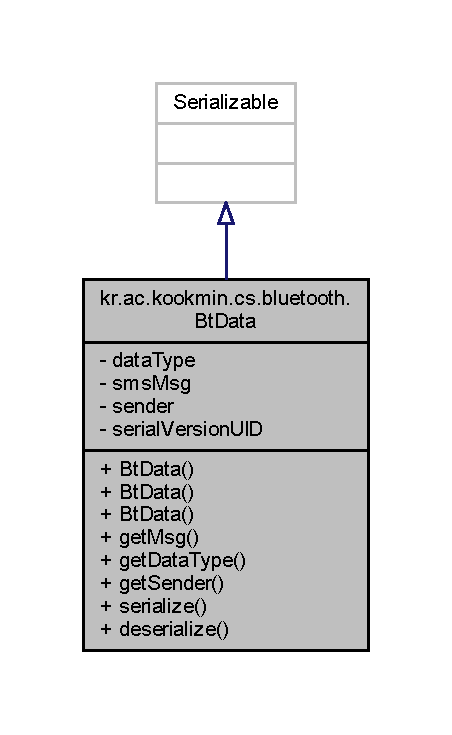
\includegraphics[width=217pt]{classkr_1_1ac_1_1kookmin_1_1cs_1_1bluetooth_1_1_bt_data__inherit__graph}
\end{center}
\end{figure}


kr.\+ac.\+kookmin.\+cs.\+bluetooth.\+Bt\+Data에 대한 협력 다이어그램\+:\nopagebreak
\begin{figure}[H]
\begin{center}
\leavevmode
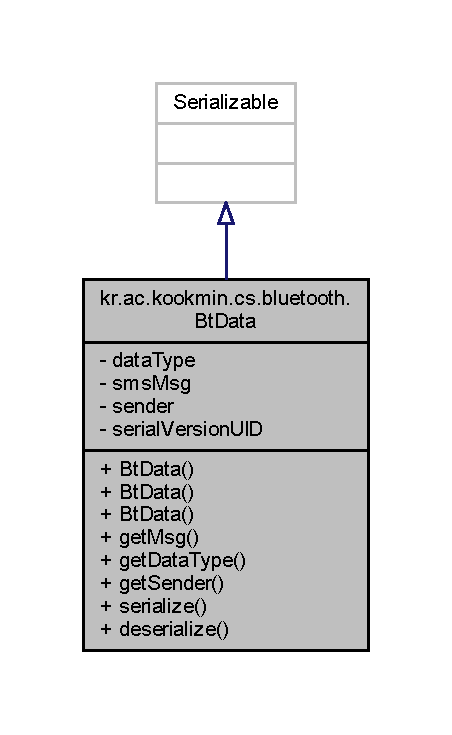
\includegraphics[width=217pt]{classkr_1_1ac_1_1kookmin_1_1cs_1_1bluetooth_1_1_bt_data__coll__graph}
\end{center}
\end{figure}
\subsection*{Public 멤버 함수}
\begin{DoxyCompactItemize}
\item 
\hyperlink{classkr_1_1ac_1_1kookmin_1_1cs_1_1bluetooth_1_1_bt_data_ae6593841e31077f20d0bc233b60a9a2f}{Bt\+Data} ()
\begin{DoxyCompactList}\small\item\em This method is constructor. and It initializes the value of an instance. \end{DoxyCompactList}\item 
\hyperlink{classkr_1_1ac_1_1kookmin_1_1cs_1_1bluetooth_1_1_bt_data_aa0a4fd989f0eb9f6f3493a76ae23608a}{Bt\+Data} (int type)
\begin{DoxyCompactList}\small\item\em This method is constructor. and It initializes the value of an instance as parameter. \end{DoxyCompactList}\item 
\hyperlink{classkr_1_1ac_1_1kookmin_1_1cs_1_1bluetooth_1_1_bt_data_a61575981c4de913ce7fd0cd4b1d136e1}{Bt\+Data} (int type, String msg, String \hyperlink{classkr_1_1ac_1_1kookmin_1_1cs_1_1bluetooth_1_1_bt_data_ab940a1cb2ab153b6fce841ee88e07b0b}{sender})
\begin{DoxyCompactList}\small\item\em This method is constructor. and It initializes the value of an instance as parameters. \end{DoxyCompactList}\item 
String \hyperlink{classkr_1_1ac_1_1kookmin_1_1cs_1_1bluetooth_1_1_bt_data_af5b8fc603edec5fa24ff0be71424c45b}{get\+Msg} ()
\item 
int \hyperlink{classkr_1_1ac_1_1kookmin_1_1cs_1_1bluetooth_1_1_bt_data_afa5370a615b4826b88869b62a510c310}{get\+Data\+Type} ()
\item 
String \hyperlink{classkr_1_1ac_1_1kookmin_1_1cs_1_1bluetooth_1_1_bt_data_a3d2bc06cc574507b11a4b8c8f2759bb8}{get\+Sender} ()
\end{DoxyCompactItemize}
\subsection*{정적 Public 멤버 함수}
\begin{DoxyCompactItemize}
\item 
static byte\mbox{[}$\,$\mbox{]} \hyperlink{classkr_1_1ac_1_1kookmin_1_1cs_1_1bluetooth_1_1_bt_data_ae0cad29a77ce0fd52299ff97b46b4a55}{serialize} (Object obj)  throws I\+O\+Exception 
\begin{DoxyCompactList}\small\item\em This method is serialize the object data to a byte array . \end{DoxyCompactList}\item 
static Object \hyperlink{classkr_1_1ac_1_1kookmin_1_1cs_1_1bluetooth_1_1_bt_data_aa48984d83a0347d73de8dc6ac706b5df}{deserialize} (byte\mbox{[}$\,$\mbox{]} data)  throws I\+O\+Exception, Class\+Not\+Found\+Exception 
\begin{DoxyCompactList}\small\item\em This method is deserialize the byte array as object data. \end{DoxyCompactList}\end{DoxyCompactItemize}
\subsection*{Private 속성}
\begin{DoxyCompactItemize}
\item 
int \hyperlink{classkr_1_1ac_1_1kookmin_1_1cs_1_1bluetooth_1_1_bt_data_ad002da4be5c1342793210a47678c1b51}{data\+Type}
\item 
String \hyperlink{classkr_1_1ac_1_1kookmin_1_1cs_1_1bluetooth_1_1_bt_data_aeca2f4bab917b5ccae3f7bed813fc2fb}{sms\+Msg}
\item 
String \hyperlink{classkr_1_1ac_1_1kookmin_1_1cs_1_1bluetooth_1_1_bt_data_ab940a1cb2ab153b6fce841ee88e07b0b}{sender}
\end{DoxyCompactItemize}
\subsection*{정적 Private 속성}
\begin{DoxyCompactItemize}
\item 
static final long \hyperlink{classkr_1_1ac_1_1kookmin_1_1cs_1_1bluetooth_1_1_bt_data_a45500b9737291a83a59755374046f647}{serial\+Version\+U\+I\+D} = 3459520869516421384\+L
\end{DoxyCompactItemize}


\subsection{상세한 설명}
This class is a data format to be transmitted in Bluetooth. 

This class has the caller information and the Bluetooth data type. and bluetooth data type is Sms data or call signal data \begin{DoxyAuthor}{작성자}
Im-\/gisung,Jo-\/\+Kwanghyeon 
\end{DoxyAuthor}


\subsection{생성자 \& 소멸자 문서화}
\hypertarget{classkr_1_1ac_1_1kookmin_1_1cs_1_1bluetooth_1_1_bt_data_ae6593841e31077f20d0bc233b60a9a2f}{}\index{kr\+::ac\+::kookmin\+::cs\+::bluetooth\+::\+Bt\+Data@{kr\+::ac\+::kookmin\+::cs\+::bluetooth\+::\+Bt\+Data}!Bt\+Data@{Bt\+Data}}
\index{Bt\+Data@{Bt\+Data}!kr\+::ac\+::kookmin\+::cs\+::bluetooth\+::\+Bt\+Data@{kr\+::ac\+::kookmin\+::cs\+::bluetooth\+::\+Bt\+Data}}
\subsubsection[{Bt\+Data}]{\setlength{\rightskip}{0pt plus 5cm}kr.\+ac.\+kookmin.\+cs.\+bluetooth.\+Bt\+Data.\+Bt\+Data (
\begin{DoxyParamCaption}
{}
\end{DoxyParamCaption}
)}\label{classkr_1_1ac_1_1kookmin_1_1cs_1_1bluetooth_1_1_bt_data_ae6593841e31077f20d0bc233b60a9a2f}


This method is constructor. and It initializes the value of an instance. 


\begin{DoxyParams}{매개변수}
{\em nothing} & \\
\hline
\end{DoxyParams}

\begin{DoxyCode}
42   \{
43     this.\hyperlink{classkr_1_1ac_1_1kookmin_1_1cs_1_1bluetooth_1_1_bt_data_ad002da4be5c1342793210a47678c1b51}{dataType}=-1;
44     this.\hyperlink{classkr_1_1ac_1_1kookmin_1_1cs_1_1bluetooth_1_1_bt_data_aeca2f4bab917b5ccae3f7bed813fc2fb}{smsMsg}=null;
45     this.\hyperlink{classkr_1_1ac_1_1kookmin_1_1cs_1_1bluetooth_1_1_bt_data_ab940a1cb2ab153b6fce841ee88e07b0b}{sender}=null;
46   \}
\end{DoxyCode}
\hypertarget{classkr_1_1ac_1_1kookmin_1_1cs_1_1bluetooth_1_1_bt_data_aa0a4fd989f0eb9f6f3493a76ae23608a}{}\index{kr\+::ac\+::kookmin\+::cs\+::bluetooth\+::\+Bt\+Data@{kr\+::ac\+::kookmin\+::cs\+::bluetooth\+::\+Bt\+Data}!Bt\+Data@{Bt\+Data}}
\index{Bt\+Data@{Bt\+Data}!kr\+::ac\+::kookmin\+::cs\+::bluetooth\+::\+Bt\+Data@{kr\+::ac\+::kookmin\+::cs\+::bluetooth\+::\+Bt\+Data}}
\subsubsection[{Bt\+Data}]{\setlength{\rightskip}{0pt plus 5cm}kr.\+ac.\+kookmin.\+cs.\+bluetooth.\+Bt\+Data.\+Bt\+Data (
\begin{DoxyParamCaption}
\item[{int}]{type}
\end{DoxyParamCaption}
)}\label{classkr_1_1ac_1_1kookmin_1_1cs_1_1bluetooth_1_1_bt_data_aa0a4fd989f0eb9f6f3493a76ae23608a}


This method is constructor. and It initializes the value of an instance as parameter. 


\begin{DoxyParams}{매개변수}
{\em type} & an integer \\
\hline
\end{DoxyParams}

\begin{DoxyCode}
53   \{
54     this.\hyperlink{classkr_1_1ac_1_1kookmin_1_1cs_1_1bluetooth_1_1_bt_data_ad002da4be5c1342793210a47678c1b51}{dataType} = type;
55     this.\hyperlink{classkr_1_1ac_1_1kookmin_1_1cs_1_1bluetooth_1_1_bt_data_aeca2f4bab917b5ccae3f7bed813fc2fb}{smsMsg}=null;
56     this.\hyperlink{classkr_1_1ac_1_1kookmin_1_1cs_1_1bluetooth_1_1_bt_data_ab940a1cb2ab153b6fce841ee88e07b0b}{sender}=null;
57   \}
\end{DoxyCode}
\hypertarget{classkr_1_1ac_1_1kookmin_1_1cs_1_1bluetooth_1_1_bt_data_a61575981c4de913ce7fd0cd4b1d136e1}{}\index{kr\+::ac\+::kookmin\+::cs\+::bluetooth\+::\+Bt\+Data@{kr\+::ac\+::kookmin\+::cs\+::bluetooth\+::\+Bt\+Data}!Bt\+Data@{Bt\+Data}}
\index{Bt\+Data@{Bt\+Data}!kr\+::ac\+::kookmin\+::cs\+::bluetooth\+::\+Bt\+Data@{kr\+::ac\+::kookmin\+::cs\+::bluetooth\+::\+Bt\+Data}}
\subsubsection[{Bt\+Data}]{\setlength{\rightskip}{0pt plus 5cm}kr.\+ac.\+kookmin.\+cs.\+bluetooth.\+Bt\+Data.\+Bt\+Data (
\begin{DoxyParamCaption}
\item[{int}]{type, }
\item[{String}]{msg, }
\item[{String}]{sender}
\end{DoxyParamCaption}
)}\label{classkr_1_1ac_1_1kookmin_1_1cs_1_1bluetooth_1_1_bt_data_a61575981c4de913ce7fd0cd4b1d136e1}


This method is constructor. and It initializes the value of an instance as parameters. 


\begin{DoxyParams}{매개변수}
{\em type} & an integer \\
\hline
{\em msg} & a String object, It is message content. \\
\hline
{\em sender} & a String object, It is a caller information . \\
\hline
\end{DoxyParams}

\begin{DoxyCode}
66   \{
67     this.\hyperlink{classkr_1_1ac_1_1kookmin_1_1cs_1_1bluetooth_1_1_bt_data_ad002da4be5c1342793210a47678c1b51}{dataType} = type;
68     this.\hyperlink{classkr_1_1ac_1_1kookmin_1_1cs_1_1bluetooth_1_1_bt_data_aeca2f4bab917b5ccae3f7bed813fc2fb}{smsMsg} = msg;
69     this.\hyperlink{classkr_1_1ac_1_1kookmin_1_1cs_1_1bluetooth_1_1_bt_data_ab940a1cb2ab153b6fce841ee88e07b0b}{sender} = \hyperlink{classkr_1_1ac_1_1kookmin_1_1cs_1_1bluetooth_1_1_bt_data_ab940a1cb2ab153b6fce841ee88e07b0b}{sender};
70   \}
\end{DoxyCode}


\subsection{멤버 함수 문서화}
\hypertarget{classkr_1_1ac_1_1kookmin_1_1cs_1_1bluetooth_1_1_bt_data_aa48984d83a0347d73de8dc6ac706b5df}{}\index{kr\+::ac\+::kookmin\+::cs\+::bluetooth\+::\+Bt\+Data@{kr\+::ac\+::kookmin\+::cs\+::bluetooth\+::\+Bt\+Data}!deserialize@{deserialize}}
\index{deserialize@{deserialize}!kr\+::ac\+::kookmin\+::cs\+::bluetooth\+::\+Bt\+Data@{kr\+::ac\+::kookmin\+::cs\+::bluetooth\+::\+Bt\+Data}}
\subsubsection[{deserialize}]{\setlength{\rightskip}{0pt plus 5cm}static Object kr.\+ac.\+kookmin.\+cs.\+bluetooth.\+Bt\+Data.\+deserialize (
\begin{DoxyParamCaption}
\item[{byte\mbox{[}$\,$\mbox{]}}]{data}
\end{DoxyParamCaption}
) throws I\+O\+Exception, Class\+Not\+Found\+Exception\hspace{0.3cm}{\ttfamily [static]}}\label{classkr_1_1ac_1_1kookmin_1_1cs_1_1bluetooth_1_1_bt_data_aa48984d83a0347d73de8dc6ac706b5df}


This method is deserialize the byte array as object data. 


\begin{DoxyParams}{매개변수}
{\em data} & a byte Array \\
\hline
\end{DoxyParams}
\begin{DoxyReturn}{반환값}
Object class 
\end{DoxyReturn}

\begin{DoxyExceptions}{예외}
{\em I\+O\+Exception} & \\
\hline
\end{DoxyExceptions}

\begin{DoxyCode}
106                                                                                            \{
107     ByteArrayInputStream in = \textcolor{keyword}{new} ByteArrayInputStream(data);
108     ObjectInputStream is = \textcolor{keyword}{new} ObjectInputStream(in);
109     \textcolor{keywordflow}{return} is.readObject();
110   \}
\end{DoxyCode}


이 함수를 호출하는 함수들에 대한 그래프입니다.\+:\nopagebreak
\begin{figure}[H]
\begin{center}
\leavevmode
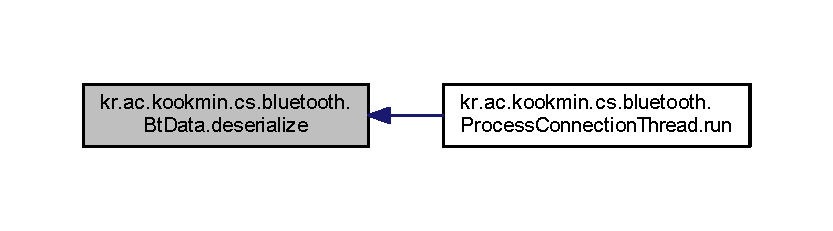
\includegraphics[width=350pt]{classkr_1_1ac_1_1kookmin_1_1cs_1_1bluetooth_1_1_bt_data_aa48984d83a0347d73de8dc6ac706b5df_icgraph}
\end{center}
\end{figure}


\hypertarget{classkr_1_1ac_1_1kookmin_1_1cs_1_1bluetooth_1_1_bt_data_afa5370a615b4826b88869b62a510c310}{}\index{kr\+::ac\+::kookmin\+::cs\+::bluetooth\+::\+Bt\+Data@{kr\+::ac\+::kookmin\+::cs\+::bluetooth\+::\+Bt\+Data}!get\+Data\+Type@{get\+Data\+Type}}
\index{get\+Data\+Type@{get\+Data\+Type}!kr\+::ac\+::kookmin\+::cs\+::bluetooth\+::\+Bt\+Data@{kr\+::ac\+::kookmin\+::cs\+::bluetooth\+::\+Bt\+Data}}
\subsubsection[{get\+Data\+Type}]{\setlength{\rightskip}{0pt plus 5cm}int kr.\+ac.\+kookmin.\+cs.\+bluetooth.\+Bt\+Data.\+get\+Data\+Type (
\begin{DoxyParamCaption}
{}
\end{DoxyParamCaption}
)}\label{classkr_1_1ac_1_1kookmin_1_1cs_1_1bluetooth_1_1_bt_data_afa5370a615b4826b88869b62a510c310}

\begin{DoxyCode}
79   \{
80     \textcolor{keywordflow}{return} \hyperlink{classkr_1_1ac_1_1kookmin_1_1cs_1_1bluetooth_1_1_bt_data_ad002da4be5c1342793210a47678c1b51}{dataType};
81   \}
\end{DoxyCode}


이 함수를 호출하는 함수들에 대한 그래프입니다.\+:\nopagebreak
\begin{figure}[H]
\begin{center}
\leavevmode
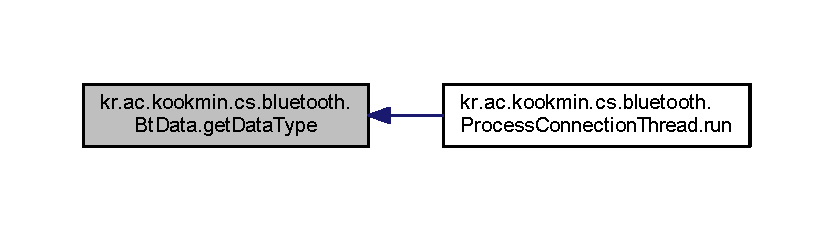
\includegraphics[width=350pt]{classkr_1_1ac_1_1kookmin_1_1cs_1_1bluetooth_1_1_bt_data_afa5370a615b4826b88869b62a510c310_icgraph}
\end{center}
\end{figure}


\hypertarget{classkr_1_1ac_1_1kookmin_1_1cs_1_1bluetooth_1_1_bt_data_af5b8fc603edec5fa24ff0be71424c45b}{}\index{kr\+::ac\+::kookmin\+::cs\+::bluetooth\+::\+Bt\+Data@{kr\+::ac\+::kookmin\+::cs\+::bluetooth\+::\+Bt\+Data}!get\+Msg@{get\+Msg}}
\index{get\+Msg@{get\+Msg}!kr\+::ac\+::kookmin\+::cs\+::bluetooth\+::\+Bt\+Data@{kr\+::ac\+::kookmin\+::cs\+::bluetooth\+::\+Bt\+Data}}
\subsubsection[{get\+Msg}]{\setlength{\rightskip}{0pt plus 5cm}String kr.\+ac.\+kookmin.\+cs.\+bluetooth.\+Bt\+Data.\+get\+Msg (
\begin{DoxyParamCaption}
{}
\end{DoxyParamCaption}
)}\label{classkr_1_1ac_1_1kookmin_1_1cs_1_1bluetooth_1_1_bt_data_af5b8fc603edec5fa24ff0be71424c45b}

\begin{DoxyCode}
74   \{
75     \textcolor{keywordflow}{return} \hyperlink{classkr_1_1ac_1_1kookmin_1_1cs_1_1bluetooth_1_1_bt_data_aeca2f4bab917b5ccae3f7bed813fc2fb}{smsMsg};
76   \}
\end{DoxyCode}


이 함수를 호출하는 함수들에 대한 그래프입니다.\+:\nopagebreak
\begin{figure}[H]
\begin{center}
\leavevmode
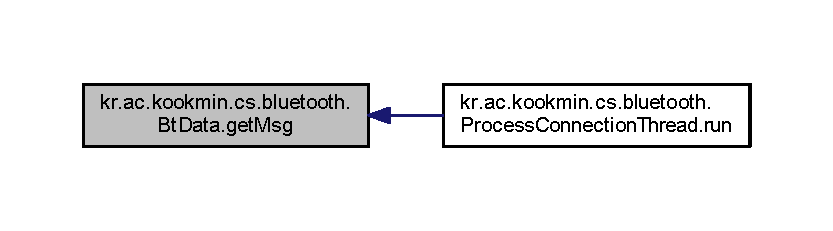
\includegraphics[width=350pt]{classkr_1_1ac_1_1kookmin_1_1cs_1_1bluetooth_1_1_bt_data_af5b8fc603edec5fa24ff0be71424c45b_icgraph}
\end{center}
\end{figure}


\hypertarget{classkr_1_1ac_1_1kookmin_1_1cs_1_1bluetooth_1_1_bt_data_a3d2bc06cc574507b11a4b8c8f2759bb8}{}\index{kr\+::ac\+::kookmin\+::cs\+::bluetooth\+::\+Bt\+Data@{kr\+::ac\+::kookmin\+::cs\+::bluetooth\+::\+Bt\+Data}!get\+Sender@{get\+Sender}}
\index{get\+Sender@{get\+Sender}!kr\+::ac\+::kookmin\+::cs\+::bluetooth\+::\+Bt\+Data@{kr\+::ac\+::kookmin\+::cs\+::bluetooth\+::\+Bt\+Data}}
\subsubsection[{get\+Sender}]{\setlength{\rightskip}{0pt plus 5cm}String kr.\+ac.\+kookmin.\+cs.\+bluetooth.\+Bt\+Data.\+get\+Sender (
\begin{DoxyParamCaption}
{}
\end{DoxyParamCaption}
)}\label{classkr_1_1ac_1_1kookmin_1_1cs_1_1bluetooth_1_1_bt_data_a3d2bc06cc574507b11a4b8c8f2759bb8}

\begin{DoxyCode}
84   \{
85     \textcolor{keywordflow}{return} \hyperlink{classkr_1_1ac_1_1kookmin_1_1cs_1_1bluetooth_1_1_bt_data_ab940a1cb2ab153b6fce841ee88e07b0b}{sender};
86   \}
\end{DoxyCode}


이 함수를 호출하는 함수들에 대한 그래프입니다.\+:\nopagebreak
\begin{figure}[H]
\begin{center}
\leavevmode
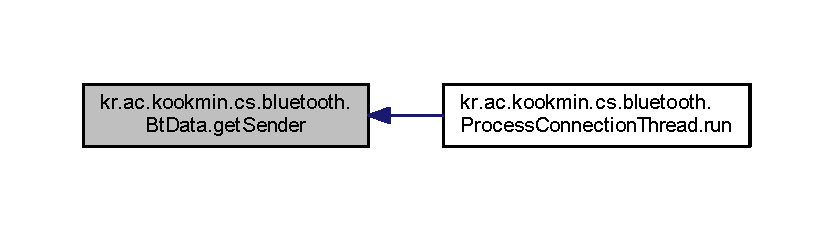
\includegraphics[width=350pt]{classkr_1_1ac_1_1kookmin_1_1cs_1_1bluetooth_1_1_bt_data_a3d2bc06cc574507b11a4b8c8f2759bb8_icgraph}
\end{center}
\end{figure}


\hypertarget{classkr_1_1ac_1_1kookmin_1_1cs_1_1bluetooth_1_1_bt_data_ae0cad29a77ce0fd52299ff97b46b4a55}{}\index{kr\+::ac\+::kookmin\+::cs\+::bluetooth\+::\+Bt\+Data@{kr\+::ac\+::kookmin\+::cs\+::bluetooth\+::\+Bt\+Data}!serialize@{serialize}}
\index{serialize@{serialize}!kr\+::ac\+::kookmin\+::cs\+::bluetooth\+::\+Bt\+Data@{kr\+::ac\+::kookmin\+::cs\+::bluetooth\+::\+Bt\+Data}}
\subsubsection[{serialize}]{\setlength{\rightskip}{0pt plus 5cm}static byte \mbox{[}$\,$\mbox{]} kr.\+ac.\+kookmin.\+cs.\+bluetooth.\+Bt\+Data.\+serialize (
\begin{DoxyParamCaption}
\item[{Object}]{obj}
\end{DoxyParamCaption}
) throws I\+O\+Exception\hspace{0.3cm}{\ttfamily [static]}}\label{classkr_1_1ac_1_1kookmin_1_1cs_1_1bluetooth_1_1_bt_data_ae0cad29a77ce0fd52299ff97b46b4a55}


This method is serialize the object data to a byte array . 


\begin{DoxyParams}{매개변수}
{\em obj} & an Object class \\
\hline
\end{DoxyParams}
\begin{DoxyReturn}{반환값}
Byte array 
\end{DoxyReturn}

\begin{DoxyExceptions}{예외}
{\em I\+O\+Exception} & \\
\hline
\end{DoxyExceptions}

\begin{DoxyCode}
94                                                                 \{
95     ByteArrayOutputStream out = \textcolor{keyword}{new} ByteArrayOutputStream();
96     ObjectOutputStream os = \textcolor{keyword}{new} ObjectOutputStream(out);
97     os.writeObject(obj);
98     \textcolor{keywordflow}{return} out.toByteArray();
99   \}
\end{DoxyCode}


이 함수를 호출하는 함수들에 대한 그래프입니다.\+:\nopagebreak
\begin{figure}[H]
\begin{center}
\leavevmode
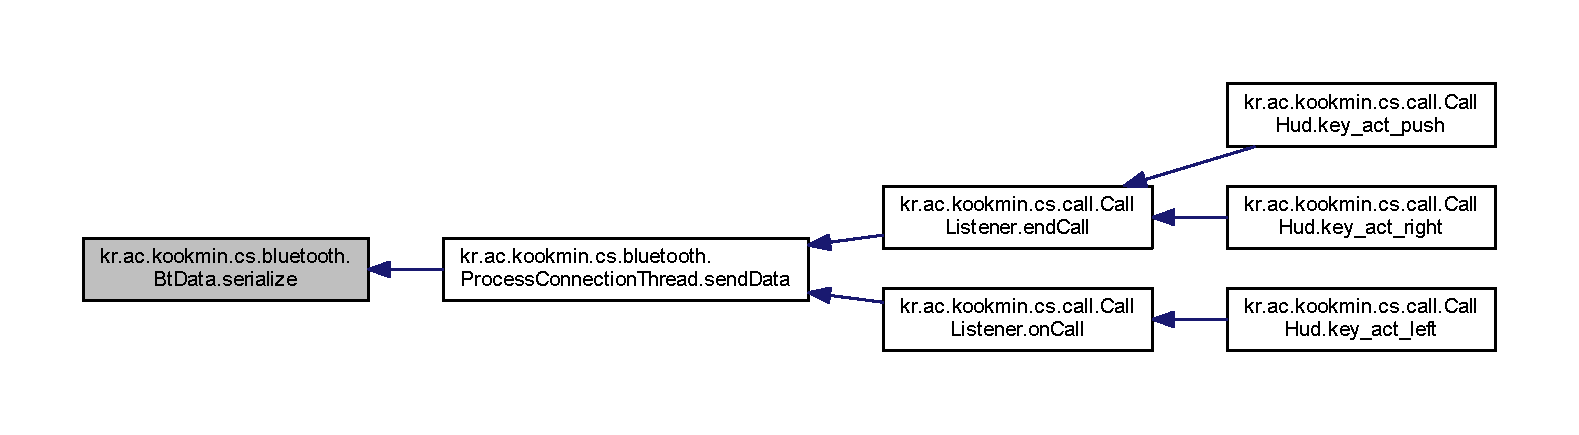
\includegraphics[width=350pt]{classkr_1_1ac_1_1kookmin_1_1cs_1_1bluetooth_1_1_bt_data_ae0cad29a77ce0fd52299ff97b46b4a55_icgraph}
\end{center}
\end{figure}




\subsection{멤버 데이타 문서화}
\hypertarget{classkr_1_1ac_1_1kookmin_1_1cs_1_1bluetooth_1_1_bt_data_ad002da4be5c1342793210a47678c1b51}{}\index{kr\+::ac\+::kookmin\+::cs\+::bluetooth\+::\+Bt\+Data@{kr\+::ac\+::kookmin\+::cs\+::bluetooth\+::\+Bt\+Data}!data\+Type@{data\+Type}}
\index{data\+Type@{data\+Type}!kr\+::ac\+::kookmin\+::cs\+::bluetooth\+::\+Bt\+Data@{kr\+::ac\+::kookmin\+::cs\+::bluetooth\+::\+Bt\+Data}}
\subsubsection[{data\+Type}]{\setlength{\rightskip}{0pt plus 5cm}int kr.\+ac.\+kookmin.\+cs.\+bluetooth.\+Bt\+Data.\+data\+Type\hspace{0.3cm}{\ttfamily [private]}}\label{classkr_1_1ac_1_1kookmin_1_1cs_1_1bluetooth_1_1_bt_data_ad002da4be5c1342793210a47678c1b51}
\hypertarget{classkr_1_1ac_1_1kookmin_1_1cs_1_1bluetooth_1_1_bt_data_ab940a1cb2ab153b6fce841ee88e07b0b}{}\index{kr\+::ac\+::kookmin\+::cs\+::bluetooth\+::\+Bt\+Data@{kr\+::ac\+::kookmin\+::cs\+::bluetooth\+::\+Bt\+Data}!sender@{sender}}
\index{sender@{sender}!kr\+::ac\+::kookmin\+::cs\+::bluetooth\+::\+Bt\+Data@{kr\+::ac\+::kookmin\+::cs\+::bluetooth\+::\+Bt\+Data}}
\subsubsection[{sender}]{\setlength{\rightskip}{0pt plus 5cm}String kr.\+ac.\+kookmin.\+cs.\+bluetooth.\+Bt\+Data.\+sender\hspace{0.3cm}{\ttfamily [private]}}\label{classkr_1_1ac_1_1kookmin_1_1cs_1_1bluetooth_1_1_bt_data_ab940a1cb2ab153b6fce841ee88e07b0b}
\hypertarget{classkr_1_1ac_1_1kookmin_1_1cs_1_1bluetooth_1_1_bt_data_a45500b9737291a83a59755374046f647}{}\index{kr\+::ac\+::kookmin\+::cs\+::bluetooth\+::\+Bt\+Data@{kr\+::ac\+::kookmin\+::cs\+::bluetooth\+::\+Bt\+Data}!serial\+Version\+U\+I\+D@{serial\+Version\+U\+I\+D}}
\index{serial\+Version\+U\+I\+D@{serial\+Version\+U\+I\+D}!kr\+::ac\+::kookmin\+::cs\+::bluetooth\+::\+Bt\+Data@{kr\+::ac\+::kookmin\+::cs\+::bluetooth\+::\+Bt\+Data}}
\subsubsection[{serial\+Version\+U\+I\+D}]{\setlength{\rightskip}{0pt plus 5cm}final long kr.\+ac.\+kookmin.\+cs.\+bluetooth.\+Bt\+Data.\+serial\+Version\+U\+I\+D = 3459520869516421384\+L\hspace{0.3cm}{\ttfamily [static]}, {\ttfamily [private]}}\label{classkr_1_1ac_1_1kookmin_1_1cs_1_1bluetooth_1_1_bt_data_a45500b9737291a83a59755374046f647}
\hypertarget{classkr_1_1ac_1_1kookmin_1_1cs_1_1bluetooth_1_1_bt_data_aeca2f4bab917b5ccae3f7bed813fc2fb}{}\index{kr\+::ac\+::kookmin\+::cs\+::bluetooth\+::\+Bt\+Data@{kr\+::ac\+::kookmin\+::cs\+::bluetooth\+::\+Bt\+Data}!sms\+Msg@{sms\+Msg}}
\index{sms\+Msg@{sms\+Msg}!kr\+::ac\+::kookmin\+::cs\+::bluetooth\+::\+Bt\+Data@{kr\+::ac\+::kookmin\+::cs\+::bluetooth\+::\+Bt\+Data}}
\subsubsection[{sms\+Msg}]{\setlength{\rightskip}{0pt plus 5cm}String kr.\+ac.\+kookmin.\+cs.\+bluetooth.\+Bt\+Data.\+sms\+Msg\hspace{0.3cm}{\ttfamily [private]}}\label{classkr_1_1ac_1_1kookmin_1_1cs_1_1bluetooth_1_1_bt_data_aeca2f4bab917b5ccae3f7bed813fc2fb}


이 클래스에 대한 문서화 페이지는 다음의 파일로부터 생성되었습니다.\+:\begin{DoxyCompactItemize}
\item 
C\+:/\+Users/\+Karasion/git/\+Capstone2015-\/\+Purple\+Ocean/src/kr/ac/kookmin/cs/bluetooth/\hyperlink{_bt_data_8java}{Bt\+Data.\+java}\end{DoxyCompactItemize}

\hypertarget{classkr_1_1ac_1_1kookmin_1_1cs_1_1call_1_1_call_hud}{}\section{kr.\+ac.\+kookmin.\+cs.\+call.\+Call\+Hud 클래스 참조}
\label{classkr_1_1ac_1_1kookmin_1_1cs_1_1call_1_1_call_hud}\index{kr.\+ac.\+kookmin.\+cs.\+call.\+Call\+Hud@{kr.\+ac.\+kookmin.\+cs.\+call.\+Call\+Hud}}


This class serves to output information related to the call to H\+U\+D.  




kr.\+ac.\+kookmin.\+cs.\+call.\+Call\+Hud에 대한 상속 다이어그램 \+: \nopagebreak
\begin{figure}[H]
\begin{center}
\leavevmode
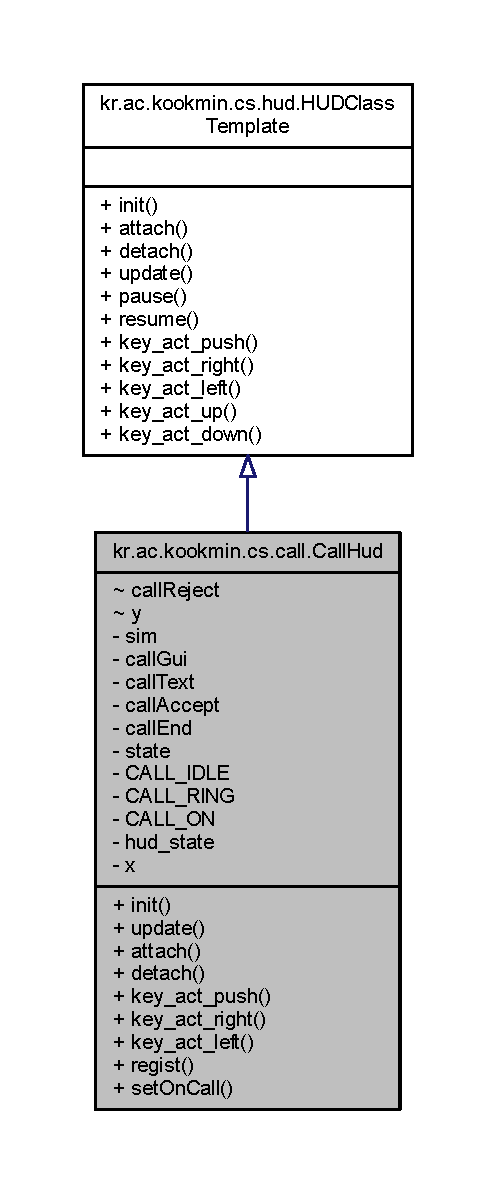
\includegraphics[height=550pt]{classkr_1_1ac_1_1kookmin_1_1cs_1_1call_1_1_call_hud__inherit__graph}
\end{center}
\end{figure}


kr.\+ac.\+kookmin.\+cs.\+call.\+Call\+Hud에 대한 협력 다이어그램\+:\nopagebreak
\begin{figure}[H]
\begin{center}
\leavevmode
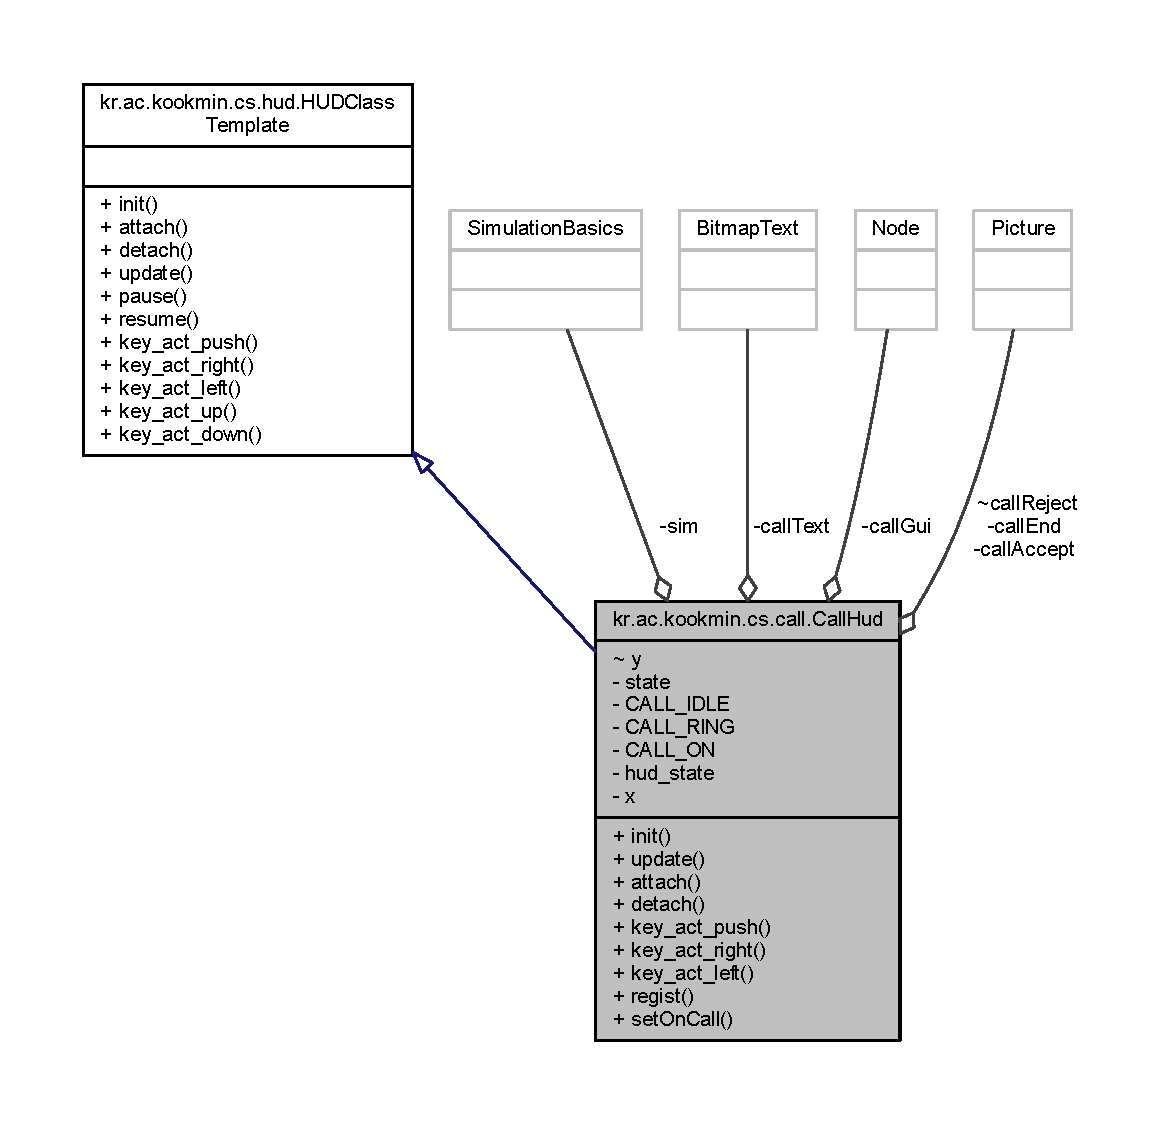
\includegraphics[width=350pt]{classkr_1_1ac_1_1kookmin_1_1cs_1_1call_1_1_call_hud__coll__graph}
\end{center}
\end{figure}
\subsection*{Public 멤버 함수}
\begin{DoxyCompactItemize}
\item 
void \hyperlink{classkr_1_1ac_1_1kookmin_1_1cs_1_1call_1_1_call_hud_ab8f90240d9719e9826ae56e387f5933d}{init} (Simulator simulator)
\begin{DoxyCompactList}\small\item\em It is a method of initializing the related elements to call. \end{DoxyCompactList}\item 
void \hyperlink{classkr_1_1ac_1_1kookmin_1_1cs_1_1call_1_1_call_hud_a28fc0dce1114387424d56d65aee6b304}{update} ()
\begin{DoxyCompactList}\small\item\em Is a method to be executed in real time on the simulator . \end{DoxyCompactList}\item 
void \hyperlink{classkr_1_1ac_1_1kookmin_1_1cs_1_1call_1_1_call_hud_a647affa35bd2b8f70f6e785f817e8082}{attach} ()
\begin{DoxyCompactList}\small\item\em This method attach the node associated with the call to simulator. \end{DoxyCompactList}\item 
void \hyperlink{classkr_1_1ac_1_1kookmin_1_1cs_1_1call_1_1_call_hud_a3f58fc64836793d7010a1d46fa787e0d}{detach} ()
\begin{DoxyCompactList}\small\item\em This method detach the node associated with the call to simulator. \end{DoxyCompactList}\item 
void \hyperlink{classkr_1_1ac_1_1kookmin_1_1cs_1_1call_1_1_call_hud_af65157e5939fc455ae649e188e38933d}{key\+\_\+act\+\_\+push} ()
\begin{DoxyCompactList}\small\item\em When you press the push button in the G-\/\+H\+U\+B, it is a method to be executed . \end{DoxyCompactList}\item 
void \hyperlink{classkr_1_1ac_1_1kookmin_1_1cs_1_1call_1_1_call_hud_a3ecf7e9fb474bd63454ed6ffcf1a6396}{key\+\_\+act\+\_\+right} ()
\begin{DoxyCompactList}\small\item\em When you press the right button in the G-\/\+H\+U\+B, it is a method to be executed . \end{DoxyCompactList}\item 
void \hyperlink{classkr_1_1ac_1_1kookmin_1_1cs_1_1call_1_1_call_hud_aec9dbfa44efd5d6ae235938dbe407c48}{key\+\_\+act\+\_\+left} ()
\begin{DoxyCompactList}\small\item\em When you press the left button in the G-\/\+H\+U\+B, it is a method to be executed . \end{DoxyCompactList}\end{DoxyCompactItemize}
\subsection*{정적 Public 멤버 함수}
\begin{DoxyCompactItemize}
\item 
static void \hyperlink{classkr_1_1ac_1_1kookmin_1_1cs_1_1call_1_1_call_hud_abc601d5d5e5823dcfe2ec269a1df52d4}{regist} ()
\begin{DoxyCompactList}\small\item\em This method to register an instance of class \hyperlink{classkr_1_1ac_1_1kookmin_1_1cs_1_1call_1_1_call_hud}{Call\+Hud} to H\+U\+D\+Management. \end{DoxyCompactList}\item 
static void \hyperlink{classkr_1_1ac_1_1kookmin_1_1cs_1_1call_1_1_call_hud_aa034521baf8a85af36a375906c693e47}{set\+On\+Call} ()
\begin{DoxyCompactList}\small\item\em This method is to change the layout to match the call to H\+U\+D. \end{DoxyCompactList}\end{DoxyCompactItemize}
\subsection*{정적 Private 속성}
\begin{DoxyCompactItemize}
\item 
static Simulation\+Basics \hyperlink{classkr_1_1ac_1_1kookmin_1_1cs_1_1call_1_1_call_hud_ad7b1172b6ece225becb5a5b6ca8ad291}{sim}
\item 
static Node \hyperlink{classkr_1_1ac_1_1kookmin_1_1cs_1_1call_1_1_call_hud_a04c754bf3f77ab819160e0769e5ef468}{call\+Gui}
\item 
static Bitmap\+Text \hyperlink{classkr_1_1ac_1_1kookmin_1_1cs_1_1call_1_1_call_hud_ad019cdb0ca0d81309a6f6013b3e1fbc4}{call\+Text}
\item 
static Picture \hyperlink{classkr_1_1ac_1_1kookmin_1_1cs_1_1call_1_1_call_hud_a865f02912a148dba841040f73f35afec}{call\+Accept}
\item 
static Picture \hyperlink{classkr_1_1ac_1_1kookmin_1_1cs_1_1call_1_1_call_hud_a12d3cd83d655c78a76ed3d340d106221}{call\+End}
\item 
static int \hyperlink{classkr_1_1ac_1_1kookmin_1_1cs_1_1call_1_1_call_hud_a205351e41055a51d9b1d33ee0c6d84f1}{state} = 0
\item 
static final int \hyperlink{classkr_1_1ac_1_1kookmin_1_1cs_1_1call_1_1_call_hud_acc23c947c0a464d1c09b04666057e8fc}{C\+A\+L\+L\+\_\+\+I\+D\+L\+E} = 0
\item 
static final int \hyperlink{classkr_1_1ac_1_1kookmin_1_1cs_1_1call_1_1_call_hud_a2dd996d4b86346a0bdc0ae462d94cf19}{C\+A\+L\+L\+\_\+\+R\+I\+N\+G} = 1
\item 
static final int \hyperlink{classkr_1_1ac_1_1kookmin_1_1cs_1_1call_1_1_call_hud_a78497626e7b91b6242225fb43517868e}{C\+A\+L\+L\+\_\+\+O\+N} = 2
\item 
static int \hyperlink{classkr_1_1ac_1_1kookmin_1_1cs_1_1call_1_1_call_hud_af5388605062cf82753266c23f663e2eb}{hud\+\_\+state}
\item 
static int \hyperlink{classkr_1_1ac_1_1kookmin_1_1cs_1_1call_1_1_call_hud_a5fb59820575dd36c90906279886188f4}{x}
\end{DoxyCompactItemize}


\subsection{상세한 설명}
This class serves to output information related to the call to H\+U\+D. 

In the simulator , if call ringing , It is output information related to the call to the appropriate position of H\+U\+D. \begin{DoxyAuthor}{작성자}
Jo-\/kwanghyeon 
\end{DoxyAuthor}


\subsection{멤버 함수 문서화}
\hypertarget{classkr_1_1ac_1_1kookmin_1_1cs_1_1call_1_1_call_hud_a647affa35bd2b8f70f6e785f817e8082}{}\index{kr\+::ac\+::kookmin\+::cs\+::call\+::\+Call\+Hud@{kr\+::ac\+::kookmin\+::cs\+::call\+::\+Call\+Hud}!attach@{attach}}
\index{attach@{attach}!kr\+::ac\+::kookmin\+::cs\+::call\+::\+Call\+Hud@{kr\+::ac\+::kookmin\+::cs\+::call\+::\+Call\+Hud}}
\subsubsection[{attach}]{\setlength{\rightskip}{0pt plus 5cm}void kr.\+ac.\+kookmin.\+cs.\+call.\+Call\+Hud.\+attach (
\begin{DoxyParamCaption}
{}
\end{DoxyParamCaption}
)}\label{classkr_1_1ac_1_1kookmin_1_1cs_1_1call_1_1_call_hud_a647affa35bd2b8f70f6e785f817e8082}


This method attach the node associated with the call to simulator. 


\begin{DoxyParams}{매개변수}
{\em nothing} & \\
\hline
\end{DoxyParams}
\begin{DoxyReturn}{반환값}
nothing 
\end{DoxyReturn}

\begin{DoxyCode}
144   \{
145     HUDManagement.attach(\hyperlink{classkr_1_1ac_1_1kookmin_1_1cs_1_1call_1_1_call_hud_a04c754bf3f77ab819160e0769e5ef468}{callGui});
146   \}
\end{DoxyCode}


이 함수 내부에서 호출하는 함수들에 대한 그래프입니다.\+:\nopagebreak
\begin{figure}[H]
\begin{center}
\leavevmode
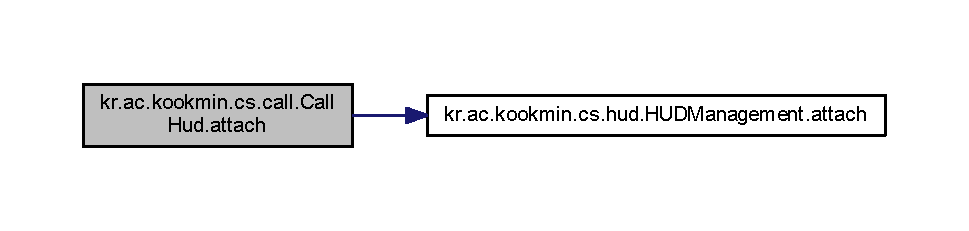
\includegraphics[width=350pt]{classkr_1_1ac_1_1kookmin_1_1cs_1_1call_1_1_call_hud_a647affa35bd2b8f70f6e785f817e8082_cgraph}
\end{center}
\end{figure}




이 함수를 호출하는 함수들에 대한 그래프입니다.\+:\nopagebreak
\begin{figure}[H]
\begin{center}
\leavevmode
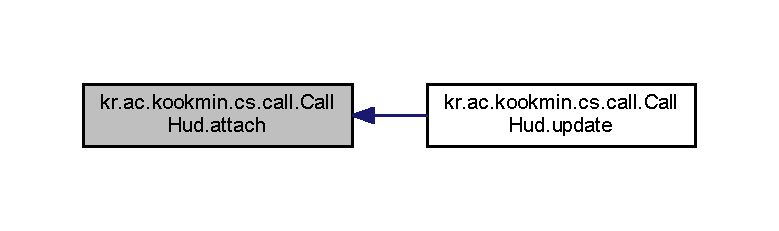
\includegraphics[width=350pt]{classkr_1_1ac_1_1kookmin_1_1cs_1_1call_1_1_call_hud_a647affa35bd2b8f70f6e785f817e8082_icgraph}
\end{center}
\end{figure}


\hypertarget{classkr_1_1ac_1_1kookmin_1_1cs_1_1call_1_1_call_hud_a3f58fc64836793d7010a1d46fa787e0d}{}\index{kr\+::ac\+::kookmin\+::cs\+::call\+::\+Call\+Hud@{kr\+::ac\+::kookmin\+::cs\+::call\+::\+Call\+Hud}!detach@{detach}}
\index{detach@{detach}!kr\+::ac\+::kookmin\+::cs\+::call\+::\+Call\+Hud@{kr\+::ac\+::kookmin\+::cs\+::call\+::\+Call\+Hud}}
\subsubsection[{detach}]{\setlength{\rightskip}{0pt plus 5cm}void kr.\+ac.\+kookmin.\+cs.\+call.\+Call\+Hud.\+detach (
\begin{DoxyParamCaption}
{}
\end{DoxyParamCaption}
)}\label{classkr_1_1ac_1_1kookmin_1_1cs_1_1call_1_1_call_hud_a3f58fc64836793d7010a1d46fa787e0d}


This method detach the node associated with the call to simulator. 


\begin{DoxyParams}{매개변수}
{\em nothing} & \\
\hline
\end{DoxyParams}
\begin{DoxyReturn}{반환값}
nothing 
\end{DoxyReturn}

\begin{DoxyCode}
154   \{
155     HUDManagement.detach(\hyperlink{classkr_1_1ac_1_1kookmin_1_1cs_1_1call_1_1_call_hud_a04c754bf3f77ab819160e0769e5ef468}{callGui});
156   \}
\end{DoxyCode}


이 함수 내부에서 호출하는 함수들에 대한 그래프입니다.\+:\nopagebreak
\begin{figure}[H]
\begin{center}
\leavevmode
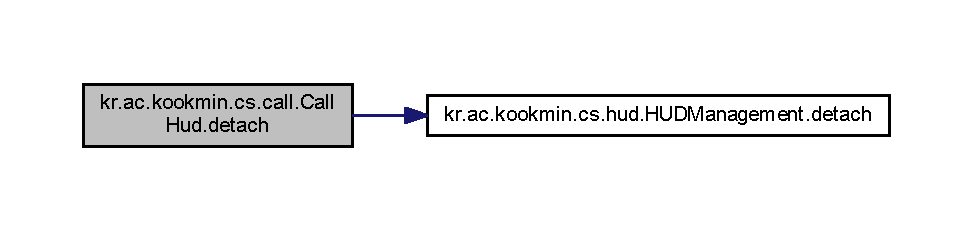
\includegraphics[width=350pt]{classkr_1_1ac_1_1kookmin_1_1cs_1_1call_1_1_call_hud_a3f58fc64836793d7010a1d46fa787e0d_cgraph}
\end{center}
\end{figure}




이 함수를 호출하는 함수들에 대한 그래프입니다.\+:\nopagebreak
\begin{figure}[H]
\begin{center}
\leavevmode
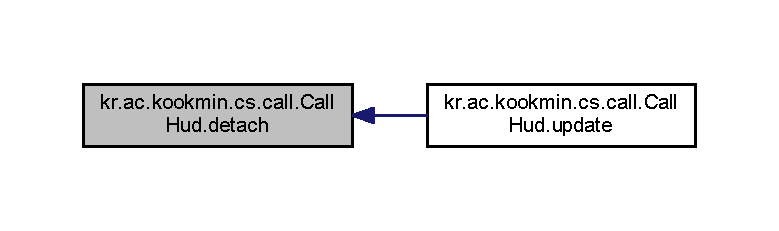
\includegraphics[width=350pt]{classkr_1_1ac_1_1kookmin_1_1cs_1_1call_1_1_call_hud_a3f58fc64836793d7010a1d46fa787e0d_icgraph}
\end{center}
\end{figure}


\hypertarget{classkr_1_1ac_1_1kookmin_1_1cs_1_1call_1_1_call_hud_ab8f90240d9719e9826ae56e387f5933d}{}\index{kr\+::ac\+::kookmin\+::cs\+::call\+::\+Call\+Hud@{kr\+::ac\+::kookmin\+::cs\+::call\+::\+Call\+Hud}!init@{init}}
\index{init@{init}!kr\+::ac\+::kookmin\+::cs\+::call\+::\+Call\+Hud@{kr\+::ac\+::kookmin\+::cs\+::call\+::\+Call\+Hud}}
\subsubsection[{init}]{\setlength{\rightskip}{0pt plus 5cm}void kr.\+ac.\+kookmin.\+cs.\+call.\+Call\+Hud.\+init (
\begin{DoxyParamCaption}
\item[{Simulator}]{simulator}
\end{DoxyParamCaption}
)}\label{classkr_1_1ac_1_1kookmin_1_1cs_1_1call_1_1_call_hud_ab8f90240d9719e9826ae56e387f5933d}


It is a method of initializing the related elements to call. 


\begin{DoxyParams}{매개변수}
{\em simulator} & a Simulator object \\
\hline
\end{DoxyParams}
\begin{DoxyReturn}{반환값}
nothing 
\end{DoxyReturn}

\begin{DoxyCode}
57   \{
58     \hyperlink{classkr_1_1ac_1_1kookmin_1_1cs_1_1call_1_1_call_hud_ad7b1172b6ece225becb5a5b6ca8ad291}{sim} = simulator;
59     \hyperlink{classkr_1_1ac_1_1kookmin_1_1cs_1_1call_1_1_call_hud_a04c754bf3f77ab819160e0769e5ef468}{callGui} = \textcolor{keyword}{new} Node(\textcolor{stringliteral}{"callGui"});
60 
61     BitmapFont font = \hyperlink{classkr_1_1ac_1_1kookmin_1_1cs_1_1call_1_1_call_hud_ad7b1172b6ece225becb5a5b6ca8ad291}{sim}.getAssetManager().loadFont(\textcolor{stringliteral}{"Interface/Fonts/MSNeoGothic/MSNeoGothic.fnt"});
62 
63     \hyperlink{classkr_1_1ac_1_1kookmin_1_1cs_1_1call_1_1_call_hud_a5fb59820575dd36c90906279886188f4}{x}=\hyperlink{classkr_1_1ac_1_1kookmin_1_1cs_1_1call_1_1_call_hud_ad7b1172b6ece225becb5a5b6ca8ad291}{sim}.getSettings().getWidth()/2;
64     y=\hyperlink{classkr_1_1ac_1_1kookmin_1_1cs_1_1call_1_1_call_hud_ad7b1172b6ece225becb5a5b6ca8ad291}{sim}.getSettings().getHeight()/2-200;
65 
66     \hyperlink{classkr_1_1ac_1_1kookmin_1_1cs_1_1call_1_1_call_hud_ad019cdb0ca0d81309a6f6013b3e1fbc4}{callText} = \textcolor{keyword}{new} BitmapText(font,\textcolor{keyword}{false});
67     \hyperlink{classkr_1_1ac_1_1kookmin_1_1cs_1_1call_1_1_call_hud_ad019cdb0ca0d81309a6f6013b3e1fbc4}{callText}.setName(\textcolor{stringliteral}{"callText"});
68     \hyperlink{classkr_1_1ac_1_1kookmin_1_1cs_1_1call_1_1_call_hud_ad019cdb0ca0d81309a6f6013b3e1fbc4}{callText}.setText(\textcolor{stringliteral}{""});
69     \hyperlink{classkr_1_1ac_1_1kookmin_1_1cs_1_1call_1_1_call_hud_ad019cdb0ca0d81309a6f6013b3e1fbc4}{callText}.setSize(font.getCharSet().getRenderedSize()+10);
70     \hyperlink{classkr_1_1ac_1_1kookmin_1_1cs_1_1call_1_1_call_hud_ad019cdb0ca0d81309a6f6013b3e1fbc4}{callText}.setColor(ColorRGBA.Yellow);
71     \hyperlink{classkr_1_1ac_1_1kookmin_1_1cs_1_1call_1_1_call_hud_ad019cdb0ca0d81309a6f6013b3e1fbc4}{callText}.setLocalTranslation(\hyperlink{classkr_1_1ac_1_1kookmin_1_1cs_1_1call_1_1_call_hud_a5fb59820575dd36c90906279886188f4}{x}-210,y,0);
72 
73     \hyperlink{classkr_1_1ac_1_1kookmin_1_1cs_1_1call_1_1_call_hud_a865f02912a148dba841040f73f35afec}{callAccept} = \textcolor{keyword}{new} Picture(\textcolor{stringliteral}{"call Accept"});
74     \hyperlink{classkr_1_1ac_1_1kookmin_1_1cs_1_1call_1_1_call_hud_a865f02912a148dba841040f73f35afec}{callAccept}.setWidth(91);
75     \hyperlink{classkr_1_1ac_1_1kookmin_1_1cs_1_1call_1_1_call_hud_a865f02912a148dba841040f73f35afec}{callAccept}.setHeight(66);
76     \hyperlink{classkr_1_1ac_1_1kookmin_1_1cs_1_1call_1_1_call_hud_a865f02912a148dba841040f73f35afec}{callAccept}.setPosition(\hyperlink{classkr_1_1ac_1_1kookmin_1_1cs_1_1call_1_1_call_hud_a5fb59820575dd36c90906279886188f4}{x}-225, y-150);
77     \hyperlink{classkr_1_1ac_1_1kookmin_1_1cs_1_1call_1_1_call_hud_a865f02912a148dba841040f73f35afec}{callAccept}.setImage(\hyperlink{classkr_1_1ac_1_1kookmin_1_1cs_1_1call_1_1_call_hud_ad7b1172b6ece225becb5a5b6ca8ad291}{sim}.getAssetManager(), \textcolor{stringliteral}{"Textures/icons/calling/call\_accept.png"}, \textcolor{keyword}{true})
      ;
78 
79     callReject = \textcolor{keyword}{new} Picture(\textcolor{stringliteral}{"call Reject"});
80     callReject.setWidth(91);
81     callReject.setHeight(66);
82     callReject.setPosition(\hyperlink{classkr_1_1ac_1_1kookmin_1_1cs_1_1call_1_1_call_hud_a5fb59820575dd36c90906279886188f4}{x}-75, y-150);
83     callReject.setImage(\hyperlink{classkr_1_1ac_1_1kookmin_1_1cs_1_1call_1_1_call_hud_ad7b1172b6ece225becb5a5b6ca8ad291}{sim}.getAssetManager(), \textcolor{stringliteral}{"Textures/icons/calling/call\_reject.png"}, \textcolor{keyword}{true});
84 
85     \hyperlink{classkr_1_1ac_1_1kookmin_1_1cs_1_1call_1_1_call_hud_a12d3cd83d655c78a76ed3d340d106221}{callEnd} = \textcolor{keyword}{new} Picture(\textcolor{stringliteral}{"call End"});
86     \hyperlink{classkr_1_1ac_1_1kookmin_1_1cs_1_1call_1_1_call_hud_a12d3cd83d655c78a76ed3d340d106221}{callEnd}.setWidth(58);
87     \hyperlink{classkr_1_1ac_1_1kookmin_1_1cs_1_1call_1_1_call_hud_a12d3cd83d655c78a76ed3d340d106221}{callEnd}.setHeight(78);
88     \hyperlink{classkr_1_1ac_1_1kookmin_1_1cs_1_1call_1_1_call_hud_a12d3cd83d655c78a76ed3d340d106221}{callEnd}.setPosition(\hyperlink{classkr_1_1ac_1_1kookmin_1_1cs_1_1call_1_1_call_hud_a5fb59820575dd36c90906279886188f4}{x}-150, y-150);
89     \hyperlink{classkr_1_1ac_1_1kookmin_1_1cs_1_1call_1_1_call_hud_a12d3cd83d655c78a76ed3d340d106221}{callEnd}.setImage(\hyperlink{classkr_1_1ac_1_1kookmin_1_1cs_1_1call_1_1_call_hud_ad7b1172b6ece225becb5a5b6ca8ad291}{sim}.getAssetManager(), \textcolor{stringliteral}{"Textures/icons/calling/call\_stop.png"}, \textcolor{keyword}{true});
90   \}
\end{DoxyCode}
\hypertarget{classkr_1_1ac_1_1kookmin_1_1cs_1_1call_1_1_call_hud_aec9dbfa44efd5d6ae235938dbe407c48}{}\index{kr\+::ac\+::kookmin\+::cs\+::call\+::\+Call\+Hud@{kr\+::ac\+::kookmin\+::cs\+::call\+::\+Call\+Hud}!key\+\_\+act\+\_\+left@{key\+\_\+act\+\_\+left}}
\index{key\+\_\+act\+\_\+left@{key\+\_\+act\+\_\+left}!kr\+::ac\+::kookmin\+::cs\+::call\+::\+Call\+Hud@{kr\+::ac\+::kookmin\+::cs\+::call\+::\+Call\+Hud}}
\subsubsection[{key\+\_\+act\+\_\+left}]{\setlength{\rightskip}{0pt plus 5cm}void kr.\+ac.\+kookmin.\+cs.\+call.\+Call\+Hud.\+key\+\_\+act\+\_\+left (
\begin{DoxyParamCaption}
{}
\end{DoxyParamCaption}
)}\label{classkr_1_1ac_1_1kookmin_1_1cs_1_1call_1_1_call_hud_aec9dbfa44efd5d6ae235938dbe407c48}


When you press the left button in the G-\/\+H\+U\+B, it is a method to be executed . 

Receive a call, if call ringing state. 
\begin{DoxyParams}{매개변수}
{\em nothing} & \\
\hline
\end{DoxyParams}
\begin{DoxyReturn}{반환값}
nothing 
\end{DoxyReturn}

\begin{DoxyCode}
199   \{
200     \textcolor{keywordflow}{if}(CallListener.getCallState() == 0)\{
201       CallListener.onCall();
202     \}
203   \}
\end{DoxyCode}


이 함수 내부에서 호출하는 함수들에 대한 그래프입니다.\+:\nopagebreak
\begin{figure}[H]
\begin{center}
\leavevmode
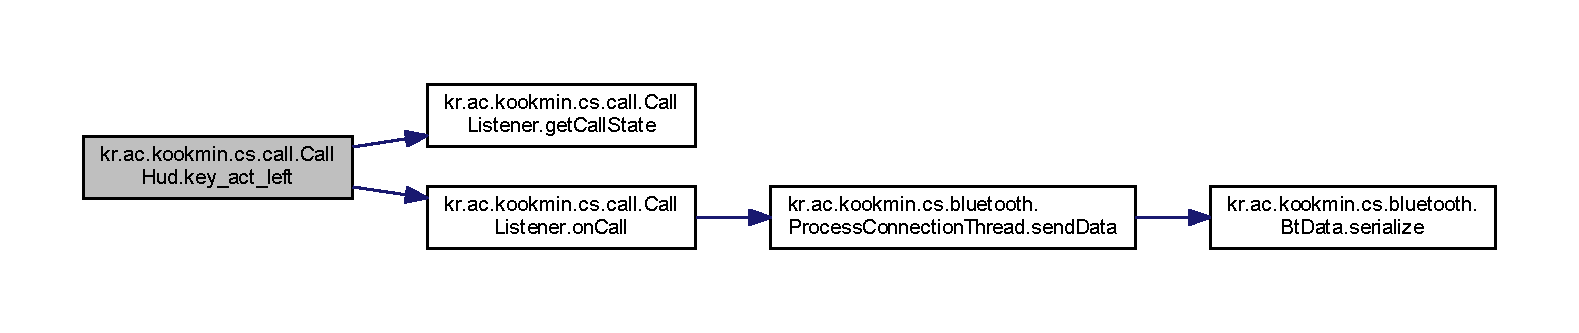
\includegraphics[width=350pt]{classkr_1_1ac_1_1kookmin_1_1cs_1_1call_1_1_call_hud_aec9dbfa44efd5d6ae235938dbe407c48_cgraph}
\end{center}
\end{figure}


\hypertarget{classkr_1_1ac_1_1kookmin_1_1cs_1_1call_1_1_call_hud_af65157e5939fc455ae649e188e38933d}{}\index{kr\+::ac\+::kookmin\+::cs\+::call\+::\+Call\+Hud@{kr\+::ac\+::kookmin\+::cs\+::call\+::\+Call\+Hud}!key\+\_\+act\+\_\+push@{key\+\_\+act\+\_\+push}}
\index{key\+\_\+act\+\_\+push@{key\+\_\+act\+\_\+push}!kr\+::ac\+::kookmin\+::cs\+::call\+::\+Call\+Hud@{kr\+::ac\+::kookmin\+::cs\+::call\+::\+Call\+Hud}}
\subsubsection[{key\+\_\+act\+\_\+push}]{\setlength{\rightskip}{0pt plus 5cm}void kr.\+ac.\+kookmin.\+cs.\+call.\+Call\+Hud.\+key\+\_\+act\+\_\+push (
\begin{DoxyParamCaption}
{}
\end{DoxyParamCaption}
)}\label{classkr_1_1ac_1_1kookmin_1_1cs_1_1call_1_1_call_hud_af65157e5939fc455ae649e188e38933d}


When you press the push button in the G-\/\+H\+U\+B, it is a method to be executed . 

To end the call , if call offhook state. 
\begin{DoxyParams}{매개변수}
{\em nothing} & \\
\hline
\end{DoxyParams}
\begin{DoxyReturn}{반환값}
nothing 
\end{DoxyReturn}

\begin{DoxyCode}
177   \{
178     \textcolor{keywordflow}{if}(CallListener.getCallState() == 1)
179       CallListener.endCall();
180   \}
\end{DoxyCode}


이 함수 내부에서 호출하는 함수들에 대한 그래프입니다.\+:\nopagebreak
\begin{figure}[H]
\begin{center}
\leavevmode
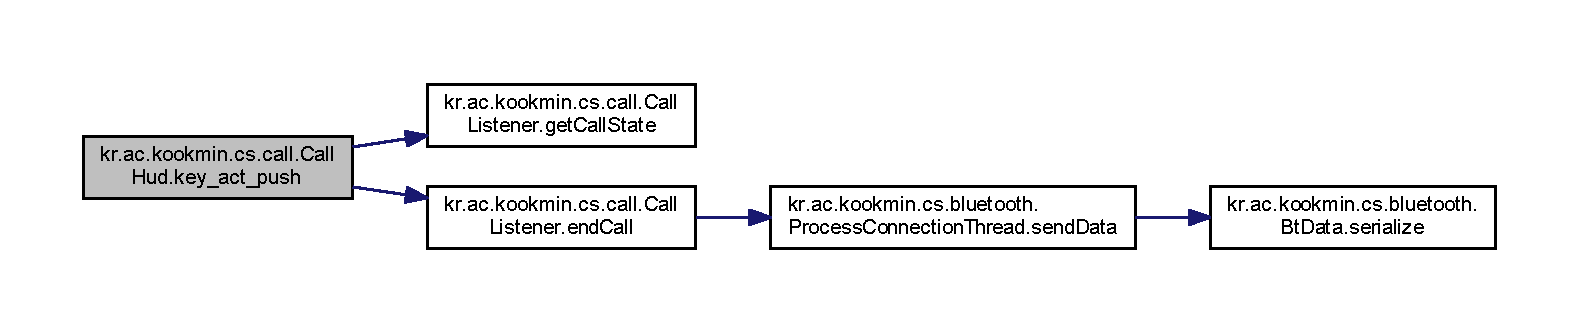
\includegraphics[width=350pt]{classkr_1_1ac_1_1kookmin_1_1cs_1_1call_1_1_call_hud_af65157e5939fc455ae649e188e38933d_cgraph}
\end{center}
\end{figure}


\hypertarget{classkr_1_1ac_1_1kookmin_1_1cs_1_1call_1_1_call_hud_a3ecf7e9fb474bd63454ed6ffcf1a6396}{}\index{kr\+::ac\+::kookmin\+::cs\+::call\+::\+Call\+Hud@{kr\+::ac\+::kookmin\+::cs\+::call\+::\+Call\+Hud}!key\+\_\+act\+\_\+right@{key\+\_\+act\+\_\+right}}
\index{key\+\_\+act\+\_\+right@{key\+\_\+act\+\_\+right}!kr\+::ac\+::kookmin\+::cs\+::call\+::\+Call\+Hud@{kr\+::ac\+::kookmin\+::cs\+::call\+::\+Call\+Hud}}
\subsubsection[{key\+\_\+act\+\_\+right}]{\setlength{\rightskip}{0pt plus 5cm}void kr.\+ac.\+kookmin.\+cs.\+call.\+Call\+Hud.\+key\+\_\+act\+\_\+right (
\begin{DoxyParamCaption}
{}
\end{DoxyParamCaption}
)}\label{classkr_1_1ac_1_1kookmin_1_1cs_1_1call_1_1_call_hud_a3ecf7e9fb474bd63454ed6ffcf1a6396}


When you press the right button in the G-\/\+H\+U\+B, it is a method to be executed . 

To end the call , if call ringing state. 
\begin{DoxyParams}{매개변수}
{\em nothing} & \\
\hline
\end{DoxyParams}
\begin{DoxyReturn}{반환값}
nothing 
\end{DoxyReturn}

\begin{DoxyCode}
188   \{
189     \textcolor{keywordflow}{if}(CallListener.getCallState() == 0)
190       CallListener.endCall();
191   \}
\end{DoxyCode}


이 함수 내부에서 호출하는 함수들에 대한 그래프입니다.\+:\nopagebreak
\begin{figure}[H]
\begin{center}
\leavevmode
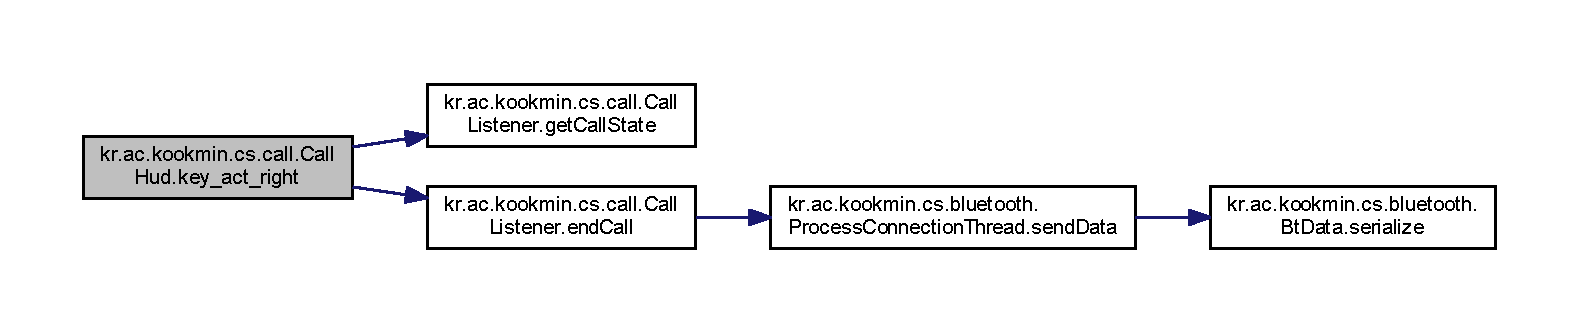
\includegraphics[width=350pt]{classkr_1_1ac_1_1kookmin_1_1cs_1_1call_1_1_call_hud_a3ecf7e9fb474bd63454ed6ffcf1a6396_cgraph}
\end{center}
\end{figure}


\hypertarget{classkr_1_1ac_1_1kookmin_1_1cs_1_1call_1_1_call_hud_abc601d5d5e5823dcfe2ec269a1df52d4}{}\index{kr\+::ac\+::kookmin\+::cs\+::call\+::\+Call\+Hud@{kr\+::ac\+::kookmin\+::cs\+::call\+::\+Call\+Hud}!regist@{regist}}
\index{regist@{regist}!kr\+::ac\+::kookmin\+::cs\+::call\+::\+Call\+Hud@{kr\+::ac\+::kookmin\+::cs\+::call\+::\+Call\+Hud}}
\subsubsection[{regist}]{\setlength{\rightskip}{0pt plus 5cm}static void kr.\+ac.\+kookmin.\+cs.\+call.\+Call\+Hud.\+regist (
\begin{DoxyParamCaption}
{}
\end{DoxyParamCaption}
)\hspace{0.3cm}{\ttfamily [static]}}\label{classkr_1_1ac_1_1kookmin_1_1cs_1_1call_1_1_call_hud_abc601d5d5e5823dcfe2ec269a1df52d4}


This method to register an instance of class \hyperlink{classkr_1_1ac_1_1kookmin_1_1cs_1_1call_1_1_call_hud}{Call\+Hud} to H\+U\+D\+Management. 


\begin{DoxyParams}{매개변수}
{\em nothing} & \\
\hline
\end{DoxyParams}
\begin{DoxyReturn}{반환값}
nothing 
\end{DoxyReturn}

\begin{DoxyCode}
98   \{
99     CallHud call = \textcolor{keyword}{new} CallHud();
100     \hyperlink{classkr_1_1ac_1_1kookmin_1_1cs_1_1call_1_1_call_hud_af5388605062cf82753266c23f663e2eb}{hud\_state} = HUDManagement.regist(call);
101   \}
\end{DoxyCode}


이 함수 내부에서 호출하는 함수들에 대한 그래프입니다.\+:\nopagebreak
\begin{figure}[H]
\begin{center}
\leavevmode
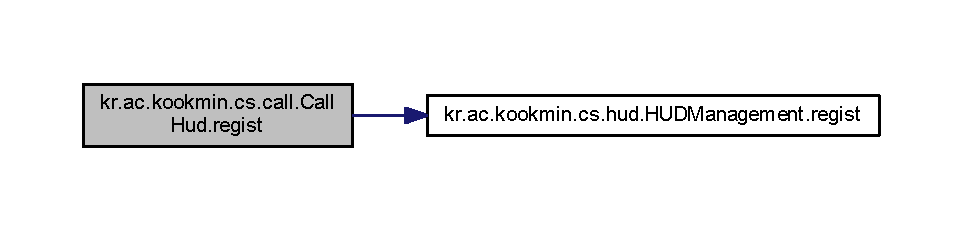
\includegraphics[width=350pt]{classkr_1_1ac_1_1kookmin_1_1cs_1_1call_1_1_call_hud_abc601d5d5e5823dcfe2ec269a1df52d4_cgraph}
\end{center}
\end{figure}




이 함수를 호출하는 함수들에 대한 그래프입니다.\+:\nopagebreak
\begin{figure}[H]
\begin{center}
\leavevmode
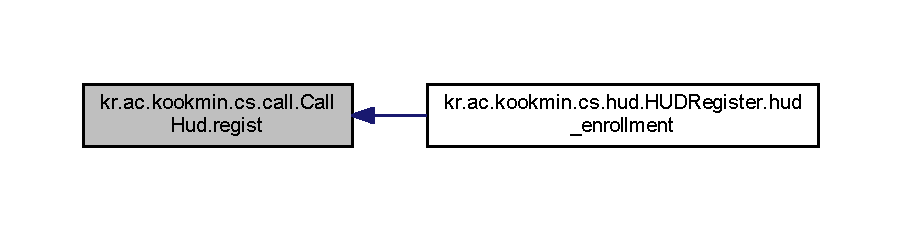
\includegraphics[width=350pt]{classkr_1_1ac_1_1kookmin_1_1cs_1_1call_1_1_call_hud_abc601d5d5e5823dcfe2ec269a1df52d4_icgraph}
\end{center}
\end{figure}


\hypertarget{classkr_1_1ac_1_1kookmin_1_1cs_1_1call_1_1_call_hud_aa034521baf8a85af36a375906c693e47}{}\index{kr\+::ac\+::kookmin\+::cs\+::call\+::\+Call\+Hud@{kr\+::ac\+::kookmin\+::cs\+::call\+::\+Call\+Hud}!set\+On\+Call@{set\+On\+Call}}
\index{set\+On\+Call@{set\+On\+Call}!kr\+::ac\+::kookmin\+::cs\+::call\+::\+Call\+Hud@{kr\+::ac\+::kookmin\+::cs\+::call\+::\+Call\+Hud}}
\subsubsection[{set\+On\+Call}]{\setlength{\rightskip}{0pt plus 5cm}static void kr.\+ac.\+kookmin.\+cs.\+call.\+Call\+Hud.\+set\+On\+Call (
\begin{DoxyParamCaption}
{}
\end{DoxyParamCaption}
)\hspace{0.3cm}{\ttfamily [static]}}\label{classkr_1_1ac_1_1kookmin_1_1cs_1_1call_1_1_call_hud_aa034521baf8a85af36a375906c693e47}


This method is to change the layout to match the call to H\+U\+D. 


\begin{DoxyParams}{매개변수}
{\em Nothing} & \\
\hline
\end{DoxyParams}
\begin{DoxyReturn}{반환값}
Nothing 
\end{DoxyReturn}

\begin{DoxyCode}
164   \{
165     \hyperlink{classkr_1_1ac_1_1kookmin_1_1cs_1_1call_1_1_call_hud_a04c754bf3f77ab819160e0769e5ef468}{callGui}.detachChild(\hyperlink{classkr_1_1ac_1_1kookmin_1_1cs_1_1call_1_1_call_hud_a865f02912a148dba841040f73f35afec}{callAccept});
166     \hyperlink{classkr_1_1ac_1_1kookmin_1_1cs_1_1call_1_1_call_hud_a04c754bf3f77ab819160e0769e5ef468}{callGui}.detachChild(callReject);
167     \hyperlink{classkr_1_1ac_1_1kookmin_1_1cs_1_1call_1_1_call_hud_a04c754bf3f77ab819160e0769e5ef468}{callGui}.attachChild(\hyperlink{classkr_1_1ac_1_1kookmin_1_1cs_1_1call_1_1_call_hud_a12d3cd83d655c78a76ed3d340d106221}{callEnd});
168   \}
\end{DoxyCode}


이 함수를 호출하는 함수들에 대한 그래프입니다.\+:\nopagebreak
\begin{figure}[H]
\begin{center}
\leavevmode
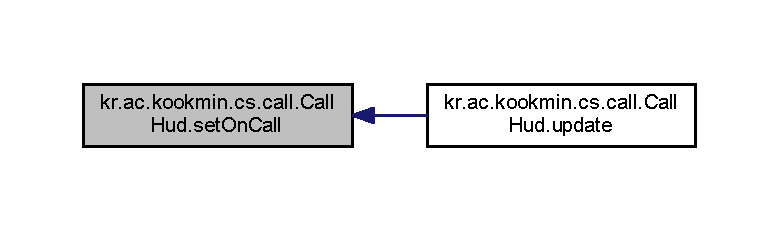
\includegraphics[width=350pt]{classkr_1_1ac_1_1kookmin_1_1cs_1_1call_1_1_call_hud_aa034521baf8a85af36a375906c693e47_icgraph}
\end{center}
\end{figure}


\hypertarget{classkr_1_1ac_1_1kookmin_1_1cs_1_1call_1_1_call_hud_a28fc0dce1114387424d56d65aee6b304}{}\index{kr\+::ac\+::kookmin\+::cs\+::call\+::\+Call\+Hud@{kr\+::ac\+::kookmin\+::cs\+::call\+::\+Call\+Hud}!update@{update}}
\index{update@{update}!kr\+::ac\+::kookmin\+::cs\+::call\+::\+Call\+Hud@{kr\+::ac\+::kookmin\+::cs\+::call\+::\+Call\+Hud}}
\subsubsection[{update}]{\setlength{\rightskip}{0pt plus 5cm}void kr.\+ac.\+kookmin.\+cs.\+call.\+Call\+Hud.\+update (
\begin{DoxyParamCaption}
{}
\end{DoxyParamCaption}
)}\label{classkr_1_1ac_1_1kookmin_1_1cs_1_1call_1_1_call_hud_a28fc0dce1114387424d56d65aee6b304}


Is a method to be executed in real time on the simulator . 

Change If this is the phone to a mobile phone , H\+U\+D state to call state. And according to the communication state , to change the layout. 
\begin{DoxyParams}{매개변수}
{\em nothing} & \\
\hline
\end{DoxyParams}
\begin{DoxyReturn}{반환값}
nothing 
\end{DoxyReturn}

\begin{DoxyCode}
111   \{     
112     \textcolor{keywordflow}{if}(CallListener.isCall() && \hyperlink{classkr_1_1ac_1_1kookmin_1_1cs_1_1call_1_1_call_hud_a205351e41055a51d9b1d33ee0c6d84f1}{state} != \hyperlink{classkr_1_1ac_1_1kookmin_1_1cs_1_1call_1_1_call_hud_a2dd996d4b86346a0bdc0ae462d94cf19}{CALL\_RING} && HUDManagement.getState() != 
      \hyperlink{classkr_1_1ac_1_1kookmin_1_1cs_1_1call_1_1_call_hud_af5388605062cf82753266c23f663e2eb}{hud\_state})\{    
113       HUDManagement.backupHUD(\hyperlink{classkr_1_1ac_1_1kookmin_1_1cs_1_1call_1_1_call_hud_af5388605062cf82753266c23f663e2eb}{hud\_state});
114       System.out.println(\textcolor{stringliteral}{"Call Hud update!"});
115       \hyperlink{classkr_1_1ac_1_1kookmin_1_1cs_1_1call_1_1_call_hud_ad019cdb0ca0d81309a6f6013b3e1fbc4}{callText}.setText(CallListener.getSender());
116       \hyperlink{classkr_1_1ac_1_1kookmin_1_1cs_1_1call_1_1_call_hud_a04c754bf3f77ab819160e0769e5ef468}{callGui}.attachChild(\hyperlink{classkr_1_1ac_1_1kookmin_1_1cs_1_1call_1_1_call_hud_ad019cdb0ca0d81309a6f6013b3e1fbc4}{callText});
117       \hyperlink{classkr_1_1ac_1_1kookmin_1_1cs_1_1call_1_1_call_hud_a04c754bf3f77ab819160e0769e5ef468}{callGui}.attachChild(\hyperlink{classkr_1_1ac_1_1kookmin_1_1cs_1_1call_1_1_call_hud_a865f02912a148dba841040f73f35afec}{callAccept});
118       \hyperlink{classkr_1_1ac_1_1kookmin_1_1cs_1_1call_1_1_call_hud_a04c754bf3f77ab819160e0769e5ef468}{callGui}.attachChild(callReject);
119       \hyperlink{classkr_1_1ac_1_1kookmin_1_1cs_1_1call_1_1_call_hud_a647affa35bd2b8f70f6e785f817e8082}{attach}();
120       HUDManagement.disableMenu(-1);
121       \hyperlink{classkr_1_1ac_1_1kookmin_1_1cs_1_1call_1_1_call_hud_a205351e41055a51d9b1d33ee0c6d84f1}{state} = \hyperlink{classkr_1_1ac_1_1kookmin_1_1cs_1_1call_1_1_call_hud_a2dd996d4b86346a0bdc0ae462d94cf19}{CALL\_RING};
122     \}
123 
124     \textcolor{keywordflow}{if}(CallListener.getCallState() == 1 && \hyperlink{classkr_1_1ac_1_1kookmin_1_1cs_1_1call_1_1_call_hud_a205351e41055a51d9b1d33ee0c6d84f1}{state} != \hyperlink{classkr_1_1ac_1_1kookmin_1_1cs_1_1call_1_1_call_hud_a78497626e7b91b6242225fb43517868e}{CALL\_ON} )\{
125       \hyperlink{classkr_1_1ac_1_1kookmin_1_1cs_1_1call_1_1_call_hud_aa034521baf8a85af36a375906c693e47}{setOnCall}();
126       \hyperlink{classkr_1_1ac_1_1kookmin_1_1cs_1_1call_1_1_call_hud_a205351e41055a51d9b1d33ee0c6d84f1}{state} = \hyperlink{classkr_1_1ac_1_1kookmin_1_1cs_1_1call_1_1_call_hud_a78497626e7b91b6242225fb43517868e}{CALL\_ON};
127     \}
128 
129     \textcolor{keywordflow}{if}(CallListener.isCall() == \textcolor{keyword}{false} && \hyperlink{classkr_1_1ac_1_1kookmin_1_1cs_1_1call_1_1_call_hud_a205351e41055a51d9b1d33ee0c6d84f1}{state} != \hyperlink{classkr_1_1ac_1_1kookmin_1_1cs_1_1call_1_1_call_hud_acc23c947c0a464d1c09b04666057e8fc}{CALL\_IDLE} && HUDManagement.getState() == 
      \hyperlink{classkr_1_1ac_1_1kookmin_1_1cs_1_1call_1_1_call_hud_af5388605062cf82753266c23f663e2eb}{hud\_state})\{
130       \hyperlink{classkr_1_1ac_1_1kookmin_1_1cs_1_1call_1_1_call_hud_a04c754bf3f77ab819160e0769e5ef468}{callGui}.detachAllChildren();
131       \hyperlink{classkr_1_1ac_1_1kookmin_1_1cs_1_1call_1_1_call_hud_a3f58fc64836793d7010a1d46fa787e0d}{detach}();
132       HUDManagement.restoreHUD();
133       HUDManagement.enableMenu();
134       \hyperlink{classkr_1_1ac_1_1kookmin_1_1cs_1_1call_1_1_call_hud_a205351e41055a51d9b1d33ee0c6d84f1}{state} = \hyperlink{classkr_1_1ac_1_1kookmin_1_1cs_1_1call_1_1_call_hud_acc23c947c0a464d1c09b04666057e8fc}{CALL\_IDLE};
135     \}
136   \}
\end{DoxyCode}


이 함수 내부에서 호출하는 함수들에 대한 그래프입니다.\+:\nopagebreak
\begin{figure}[H]
\begin{center}
\leavevmode
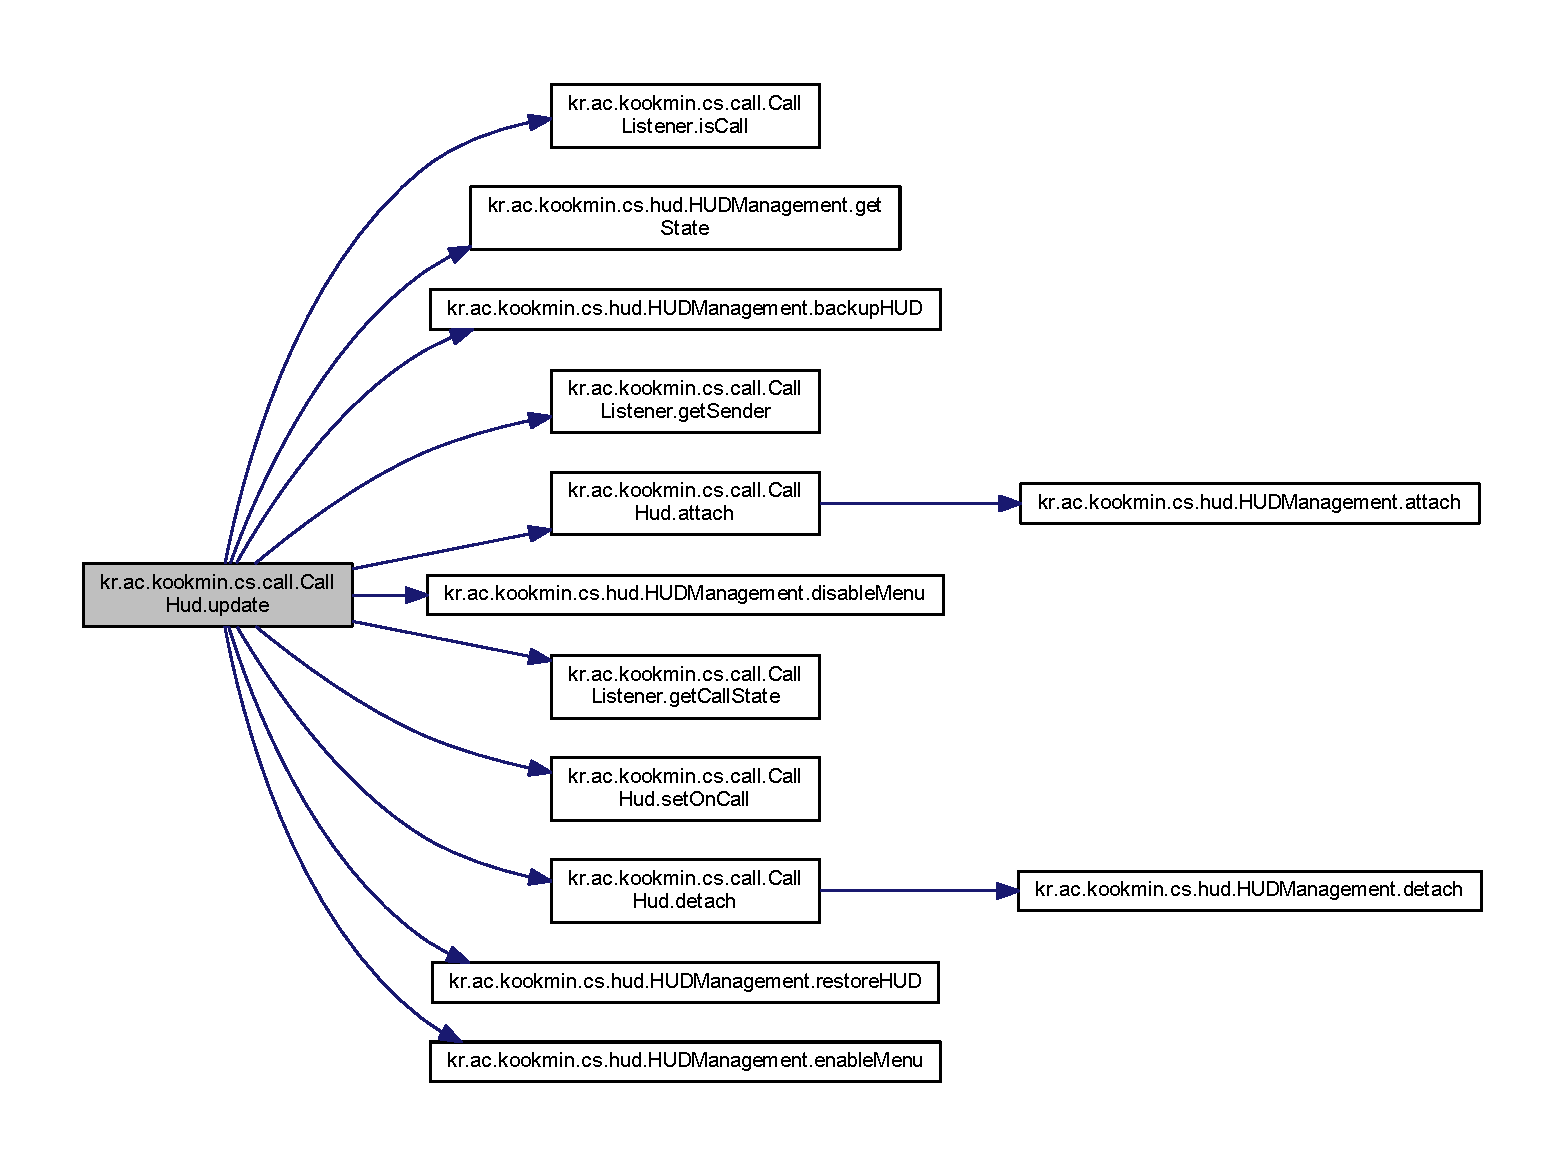
\includegraphics[width=350pt]{classkr_1_1ac_1_1kookmin_1_1cs_1_1call_1_1_call_hud_a28fc0dce1114387424d56d65aee6b304_cgraph}
\end{center}
\end{figure}




\subsection{멤버 데이타 문서화}
\hypertarget{classkr_1_1ac_1_1kookmin_1_1cs_1_1call_1_1_call_hud_acc23c947c0a464d1c09b04666057e8fc}{}\index{kr\+::ac\+::kookmin\+::cs\+::call\+::\+Call\+Hud@{kr\+::ac\+::kookmin\+::cs\+::call\+::\+Call\+Hud}!C\+A\+L\+L\+\_\+\+I\+D\+L\+E@{C\+A\+L\+L\+\_\+\+I\+D\+L\+E}}
\index{C\+A\+L\+L\+\_\+\+I\+D\+L\+E@{C\+A\+L\+L\+\_\+\+I\+D\+L\+E}!kr\+::ac\+::kookmin\+::cs\+::call\+::\+Call\+Hud@{kr\+::ac\+::kookmin\+::cs\+::call\+::\+Call\+Hud}}
\subsubsection[{C\+A\+L\+L\+\_\+\+I\+D\+L\+E}]{\setlength{\rightskip}{0pt plus 5cm}final int kr.\+ac.\+kookmin.\+cs.\+call.\+Call\+Hud.\+C\+A\+L\+L\+\_\+\+I\+D\+L\+E = 0\hspace{0.3cm}{\ttfamily [static]}, {\ttfamily [private]}}\label{classkr_1_1ac_1_1kookmin_1_1cs_1_1call_1_1_call_hud_acc23c947c0a464d1c09b04666057e8fc}
\hypertarget{classkr_1_1ac_1_1kookmin_1_1cs_1_1call_1_1_call_hud_a78497626e7b91b6242225fb43517868e}{}\index{kr\+::ac\+::kookmin\+::cs\+::call\+::\+Call\+Hud@{kr\+::ac\+::kookmin\+::cs\+::call\+::\+Call\+Hud}!C\+A\+L\+L\+\_\+\+O\+N@{C\+A\+L\+L\+\_\+\+O\+N}}
\index{C\+A\+L\+L\+\_\+\+O\+N@{C\+A\+L\+L\+\_\+\+O\+N}!kr\+::ac\+::kookmin\+::cs\+::call\+::\+Call\+Hud@{kr\+::ac\+::kookmin\+::cs\+::call\+::\+Call\+Hud}}
\subsubsection[{C\+A\+L\+L\+\_\+\+O\+N}]{\setlength{\rightskip}{0pt plus 5cm}final int kr.\+ac.\+kookmin.\+cs.\+call.\+Call\+Hud.\+C\+A\+L\+L\+\_\+\+O\+N = 2\hspace{0.3cm}{\ttfamily [static]}, {\ttfamily [private]}}\label{classkr_1_1ac_1_1kookmin_1_1cs_1_1call_1_1_call_hud_a78497626e7b91b6242225fb43517868e}
\hypertarget{classkr_1_1ac_1_1kookmin_1_1cs_1_1call_1_1_call_hud_a2dd996d4b86346a0bdc0ae462d94cf19}{}\index{kr\+::ac\+::kookmin\+::cs\+::call\+::\+Call\+Hud@{kr\+::ac\+::kookmin\+::cs\+::call\+::\+Call\+Hud}!C\+A\+L\+L\+\_\+\+R\+I\+N\+G@{C\+A\+L\+L\+\_\+\+R\+I\+N\+G}}
\index{C\+A\+L\+L\+\_\+\+R\+I\+N\+G@{C\+A\+L\+L\+\_\+\+R\+I\+N\+G}!kr\+::ac\+::kookmin\+::cs\+::call\+::\+Call\+Hud@{kr\+::ac\+::kookmin\+::cs\+::call\+::\+Call\+Hud}}
\subsubsection[{C\+A\+L\+L\+\_\+\+R\+I\+N\+G}]{\setlength{\rightskip}{0pt plus 5cm}final int kr.\+ac.\+kookmin.\+cs.\+call.\+Call\+Hud.\+C\+A\+L\+L\+\_\+\+R\+I\+N\+G = 1\hspace{0.3cm}{\ttfamily [static]}, {\ttfamily [private]}}\label{classkr_1_1ac_1_1kookmin_1_1cs_1_1call_1_1_call_hud_a2dd996d4b86346a0bdc0ae462d94cf19}
\hypertarget{classkr_1_1ac_1_1kookmin_1_1cs_1_1call_1_1_call_hud_a865f02912a148dba841040f73f35afec}{}\index{kr\+::ac\+::kookmin\+::cs\+::call\+::\+Call\+Hud@{kr\+::ac\+::kookmin\+::cs\+::call\+::\+Call\+Hud}!call\+Accept@{call\+Accept}}
\index{call\+Accept@{call\+Accept}!kr\+::ac\+::kookmin\+::cs\+::call\+::\+Call\+Hud@{kr\+::ac\+::kookmin\+::cs\+::call\+::\+Call\+Hud}}
\subsubsection[{call\+Accept}]{\setlength{\rightskip}{0pt plus 5cm}Picture kr.\+ac.\+kookmin.\+cs.\+call.\+Call\+Hud.\+call\+Accept\hspace{0.3cm}{\ttfamily [static]}, {\ttfamily [private]}}\label{classkr_1_1ac_1_1kookmin_1_1cs_1_1call_1_1_call_hud_a865f02912a148dba841040f73f35afec}
\hypertarget{classkr_1_1ac_1_1kookmin_1_1cs_1_1call_1_1_call_hud_a12d3cd83d655c78a76ed3d340d106221}{}\index{kr\+::ac\+::kookmin\+::cs\+::call\+::\+Call\+Hud@{kr\+::ac\+::kookmin\+::cs\+::call\+::\+Call\+Hud}!call\+End@{call\+End}}
\index{call\+End@{call\+End}!kr\+::ac\+::kookmin\+::cs\+::call\+::\+Call\+Hud@{kr\+::ac\+::kookmin\+::cs\+::call\+::\+Call\+Hud}}
\subsubsection[{call\+End}]{\setlength{\rightskip}{0pt plus 5cm}Picture kr.\+ac.\+kookmin.\+cs.\+call.\+Call\+Hud.\+call\+End\hspace{0.3cm}{\ttfamily [static]}, {\ttfamily [private]}}\label{classkr_1_1ac_1_1kookmin_1_1cs_1_1call_1_1_call_hud_a12d3cd83d655c78a76ed3d340d106221}
\hypertarget{classkr_1_1ac_1_1kookmin_1_1cs_1_1call_1_1_call_hud_a04c754bf3f77ab819160e0769e5ef468}{}\index{kr\+::ac\+::kookmin\+::cs\+::call\+::\+Call\+Hud@{kr\+::ac\+::kookmin\+::cs\+::call\+::\+Call\+Hud}!call\+Gui@{call\+Gui}}
\index{call\+Gui@{call\+Gui}!kr\+::ac\+::kookmin\+::cs\+::call\+::\+Call\+Hud@{kr\+::ac\+::kookmin\+::cs\+::call\+::\+Call\+Hud}}
\subsubsection[{call\+Gui}]{\setlength{\rightskip}{0pt plus 5cm}Node kr.\+ac.\+kookmin.\+cs.\+call.\+Call\+Hud.\+call\+Gui\hspace{0.3cm}{\ttfamily [static]}, {\ttfamily [private]}}\label{classkr_1_1ac_1_1kookmin_1_1cs_1_1call_1_1_call_hud_a04c754bf3f77ab819160e0769e5ef468}
\hypertarget{classkr_1_1ac_1_1kookmin_1_1cs_1_1call_1_1_call_hud_ad019cdb0ca0d81309a6f6013b3e1fbc4}{}\index{kr\+::ac\+::kookmin\+::cs\+::call\+::\+Call\+Hud@{kr\+::ac\+::kookmin\+::cs\+::call\+::\+Call\+Hud}!call\+Text@{call\+Text}}
\index{call\+Text@{call\+Text}!kr\+::ac\+::kookmin\+::cs\+::call\+::\+Call\+Hud@{kr\+::ac\+::kookmin\+::cs\+::call\+::\+Call\+Hud}}
\subsubsection[{call\+Text}]{\setlength{\rightskip}{0pt plus 5cm}Bitmap\+Text kr.\+ac.\+kookmin.\+cs.\+call.\+Call\+Hud.\+call\+Text\hspace{0.3cm}{\ttfamily [static]}, {\ttfamily [private]}}\label{classkr_1_1ac_1_1kookmin_1_1cs_1_1call_1_1_call_hud_ad019cdb0ca0d81309a6f6013b3e1fbc4}
\hypertarget{classkr_1_1ac_1_1kookmin_1_1cs_1_1call_1_1_call_hud_af5388605062cf82753266c23f663e2eb}{}\index{kr\+::ac\+::kookmin\+::cs\+::call\+::\+Call\+Hud@{kr\+::ac\+::kookmin\+::cs\+::call\+::\+Call\+Hud}!hud\+\_\+state@{hud\+\_\+state}}
\index{hud\+\_\+state@{hud\+\_\+state}!kr\+::ac\+::kookmin\+::cs\+::call\+::\+Call\+Hud@{kr\+::ac\+::kookmin\+::cs\+::call\+::\+Call\+Hud}}
\subsubsection[{hud\+\_\+state}]{\setlength{\rightskip}{0pt plus 5cm}int kr.\+ac.\+kookmin.\+cs.\+call.\+Call\+Hud.\+hud\+\_\+state\hspace{0.3cm}{\ttfamily [static]}, {\ttfamily [private]}}\label{classkr_1_1ac_1_1kookmin_1_1cs_1_1call_1_1_call_hud_af5388605062cf82753266c23f663e2eb}
\hypertarget{classkr_1_1ac_1_1kookmin_1_1cs_1_1call_1_1_call_hud_ad7b1172b6ece225becb5a5b6ca8ad291}{}\index{kr\+::ac\+::kookmin\+::cs\+::call\+::\+Call\+Hud@{kr\+::ac\+::kookmin\+::cs\+::call\+::\+Call\+Hud}!sim@{sim}}
\index{sim@{sim}!kr\+::ac\+::kookmin\+::cs\+::call\+::\+Call\+Hud@{kr\+::ac\+::kookmin\+::cs\+::call\+::\+Call\+Hud}}
\subsubsection[{sim}]{\setlength{\rightskip}{0pt plus 5cm}Simulation\+Basics kr.\+ac.\+kookmin.\+cs.\+call.\+Call\+Hud.\+sim\hspace{0.3cm}{\ttfamily [static]}, {\ttfamily [private]}}\label{classkr_1_1ac_1_1kookmin_1_1cs_1_1call_1_1_call_hud_ad7b1172b6ece225becb5a5b6ca8ad291}
\hypertarget{classkr_1_1ac_1_1kookmin_1_1cs_1_1call_1_1_call_hud_a205351e41055a51d9b1d33ee0c6d84f1}{}\index{kr\+::ac\+::kookmin\+::cs\+::call\+::\+Call\+Hud@{kr\+::ac\+::kookmin\+::cs\+::call\+::\+Call\+Hud}!state@{state}}
\index{state@{state}!kr\+::ac\+::kookmin\+::cs\+::call\+::\+Call\+Hud@{kr\+::ac\+::kookmin\+::cs\+::call\+::\+Call\+Hud}}
\subsubsection[{state}]{\setlength{\rightskip}{0pt plus 5cm}int kr.\+ac.\+kookmin.\+cs.\+call.\+Call\+Hud.\+state = 0\hspace{0.3cm}{\ttfamily [static]}, {\ttfamily [private]}}\label{classkr_1_1ac_1_1kookmin_1_1cs_1_1call_1_1_call_hud_a205351e41055a51d9b1d33ee0c6d84f1}
\hypertarget{classkr_1_1ac_1_1kookmin_1_1cs_1_1call_1_1_call_hud_a5fb59820575dd36c90906279886188f4}{}\index{kr\+::ac\+::kookmin\+::cs\+::call\+::\+Call\+Hud@{kr\+::ac\+::kookmin\+::cs\+::call\+::\+Call\+Hud}!x@{x}}
\index{x@{x}!kr\+::ac\+::kookmin\+::cs\+::call\+::\+Call\+Hud@{kr\+::ac\+::kookmin\+::cs\+::call\+::\+Call\+Hud}}
\subsubsection[{x}]{\setlength{\rightskip}{0pt plus 5cm}int kr.\+ac.\+kookmin.\+cs.\+call.\+Call\+Hud.\+x\hspace{0.3cm}{\ttfamily [static]}, {\ttfamily [private]}}\label{classkr_1_1ac_1_1kookmin_1_1cs_1_1call_1_1_call_hud_a5fb59820575dd36c90906279886188f4}


이 클래스에 대한 문서화 페이지는 다음의 파일로부터 생성되었습니다.\+:\begin{DoxyCompactItemize}
\item 
C\+:/\+Users/\+Karasion/git/\+Capstone2015-\/\+Purple\+Ocean/src/kr/ac/kookmin/cs/call/\hyperlink{_call_hud_8java}{Call\+Hud.\+java}\end{DoxyCompactItemize}

\hypertarget{classkr_1_1ac_1_1kookmin_1_1cs_1_1call_1_1_call_listener}{}\section{kr.\+ac.\+kookmin.\+cs.\+call.\+Call\+Listener 클래스 참조}
\label{classkr_1_1ac_1_1kookmin_1_1cs_1_1call_1_1_call_listener}\index{kr.\+ac.\+kookmin.\+cs.\+call.\+Call\+Listener@{kr.\+ac.\+kookmin.\+cs.\+call.\+Call\+Listener}}


It is a class related to call.  




kr.\+ac.\+kookmin.\+cs.\+call.\+Call\+Listener에 대한 협력 다이어그램\+:\nopagebreak
\begin{figure}[H]
\begin{center}
\leavevmode
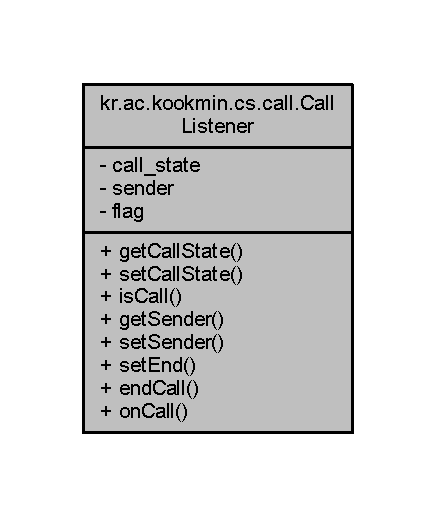
\includegraphics[width=209pt]{classkr_1_1ac_1_1kookmin_1_1cs_1_1call_1_1_call_listener__coll__graph}
\end{center}
\end{figure}
\subsection*{정적 Public 멤버 함수}
\begin{DoxyCompactItemize}
\item 
static int \hyperlink{classkr_1_1ac_1_1kookmin_1_1cs_1_1call_1_1_call_listener_a7fceefa2570760dde2970fe8ffd8ceae}{get\+Call\+State} ()
\item 
static void \hyperlink{classkr_1_1ac_1_1kookmin_1_1cs_1_1call_1_1_call_listener_aec282649d8f8b5690d1bf7c5e7e73781}{set\+Call\+State} (int state)
\item 
static boolean \hyperlink{classkr_1_1ac_1_1kookmin_1_1cs_1_1call_1_1_call_listener_a886a6345c6f2ed74e64914984e270f6d}{is\+Call} ()
\begin{DoxyCompactList}\small\item\em Method to check whether or not the call state. \end{DoxyCompactList}\item 
static String \hyperlink{classkr_1_1ac_1_1kookmin_1_1cs_1_1call_1_1_call_listener_afcbd7b4289361b3d773cafa29f033f89}{get\+Sender} ()
\item 
static void \hyperlink{classkr_1_1ac_1_1kookmin_1_1cs_1_1call_1_1_call_listener_a4a5fc9ec67f36eed4c2e934875abf007}{set\+Sender} (String \hyperlink{classkr_1_1ac_1_1kookmin_1_1cs_1_1call_1_1_call_listener_a87caf58642cf13014f53edb0fdcda07b}{sender})
\item 
static void \hyperlink{classkr_1_1ac_1_1kookmin_1_1cs_1_1call_1_1_call_listener_a11abb308347a972e68de7eed6b569a7b}{set\+End} ()
\begin{DoxyCompactList}\small\item\em It wants to change to the end state of the call. \end{DoxyCompactList}\item 
static void \hyperlink{classkr_1_1ac_1_1kookmin_1_1cs_1_1call_1_1_call_listener_a8b9c6d3b52e1fe1e080f265eed49f0a9}{end\+Call} ()
\begin{DoxyCompactList}\small\item\em It send a message to reject a phone call to the mobile in this method. \end{DoxyCompactList}\item 
static void \hyperlink{classkr_1_1ac_1_1kookmin_1_1cs_1_1call_1_1_call_listener_a2fdc9350dd23a0b6a706919b2cd2c59e}{on\+Call} ()
\begin{DoxyCompactList}\small\item\em It sends a message of receiving a phone call to the mobile in this method. \end{DoxyCompactList}\end{DoxyCompactItemize}
\subsection*{정적 Private 속성}
\begin{DoxyCompactItemize}
\item 
static int \hyperlink{classkr_1_1ac_1_1kookmin_1_1cs_1_1call_1_1_call_listener_a03420a995d78c4421f4fe92b75be5647}{call\+\_\+state} = 0
\item 
static String \hyperlink{classkr_1_1ac_1_1kookmin_1_1cs_1_1call_1_1_call_listener_a87caf58642cf13014f53edb0fdcda07b}{sender} = \char`\"{}\char`\"{}
\item 
static boolean \hyperlink{classkr_1_1ac_1_1kookmin_1_1cs_1_1call_1_1_call_listener_a43a92315d34bbf897048aea788679fbc}{flag} = false
\end{DoxyCompactItemize}


\subsection{상세한 설명}
It is a class related to call. 

This class is synchronized with the call state of the mobile . And the call action is implemented. \begin{DoxyAuthor}{작성자}
Jo-\/kwanghyeon 
\end{DoxyAuthor}


\subsection{멤버 함수 문서화}
\hypertarget{classkr_1_1ac_1_1kookmin_1_1cs_1_1call_1_1_call_listener_a8b9c6d3b52e1fe1e080f265eed49f0a9}{}\index{kr\+::ac\+::kookmin\+::cs\+::call\+::\+Call\+Listener@{kr\+::ac\+::kookmin\+::cs\+::call\+::\+Call\+Listener}!end\+Call@{end\+Call}}
\index{end\+Call@{end\+Call}!kr\+::ac\+::kookmin\+::cs\+::call\+::\+Call\+Listener@{kr\+::ac\+::kookmin\+::cs\+::call\+::\+Call\+Listener}}
\subsubsection[{end\+Call}]{\setlength{\rightskip}{0pt plus 5cm}static void kr.\+ac.\+kookmin.\+cs.\+call.\+Call\+Listener.\+end\+Call (
\begin{DoxyParamCaption}
{}
\end{DoxyParamCaption}
)\hspace{0.3cm}{\ttfamily [static]}}\label{classkr_1_1ac_1_1kookmin_1_1cs_1_1call_1_1_call_listener_a8b9c6d3b52e1fe1e080f265eed49f0a9}


It send a message to reject a phone call to the mobile in this method. 


\begin{DoxyParams}{매개변수}
{\em Nothing} & \\
\hline
\end{DoxyParams}
\begin{DoxyReturn}{반환값}
Nothing 
\end{DoxyReturn}

\begin{DoxyCode}
69                               \{
70     ProcessConnectionThread.sendData(\textcolor{stringliteral}{"endCall"});
71     \hyperlink{classkr_1_1ac_1_1kookmin_1_1cs_1_1call_1_1_call_listener_a03420a995d78c4421f4fe92b75be5647}{call\_state} = 0;
72     \hyperlink{classkr_1_1ac_1_1kookmin_1_1cs_1_1call_1_1_call_listener_a43a92315d34bbf897048aea788679fbc}{flag} = \textcolor{keyword}{false};
73   \}
\end{DoxyCode}


이 함수 내부에서 호출하는 함수들에 대한 그래프입니다.\+:\nopagebreak
\begin{figure}[H]
\begin{center}
\leavevmode
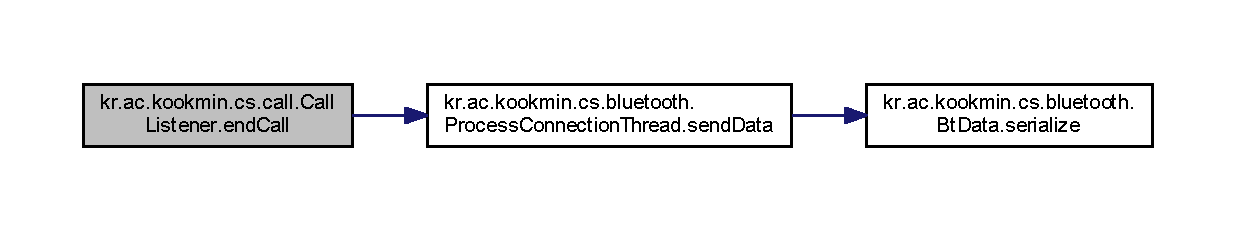
\includegraphics[width=350pt]{classkr_1_1ac_1_1kookmin_1_1cs_1_1call_1_1_call_listener_a8b9c6d3b52e1fe1e080f265eed49f0a9_cgraph}
\end{center}
\end{figure}




이 함수를 호출하는 함수들에 대한 그래프입니다.\+:\nopagebreak
\begin{figure}[H]
\begin{center}
\leavevmode
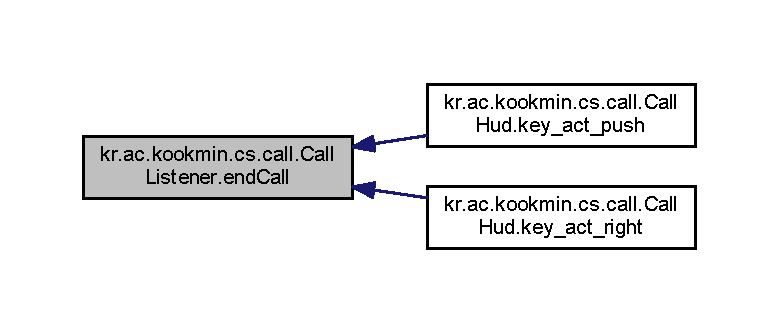
\includegraphics[width=350pt]{classkr_1_1ac_1_1kookmin_1_1cs_1_1call_1_1_call_listener_a8b9c6d3b52e1fe1e080f265eed49f0a9_icgraph}
\end{center}
\end{figure}


\hypertarget{classkr_1_1ac_1_1kookmin_1_1cs_1_1call_1_1_call_listener_a7fceefa2570760dde2970fe8ffd8ceae}{}\index{kr\+::ac\+::kookmin\+::cs\+::call\+::\+Call\+Listener@{kr\+::ac\+::kookmin\+::cs\+::call\+::\+Call\+Listener}!get\+Call\+State@{get\+Call\+State}}
\index{get\+Call\+State@{get\+Call\+State}!kr\+::ac\+::kookmin\+::cs\+::call\+::\+Call\+Listener@{kr\+::ac\+::kookmin\+::cs\+::call\+::\+Call\+Listener}}
\subsubsection[{get\+Call\+State}]{\setlength{\rightskip}{0pt plus 5cm}static int kr.\+ac.\+kookmin.\+cs.\+call.\+Call\+Listener.\+get\+Call\+State (
\begin{DoxyParamCaption}
{}
\end{DoxyParamCaption}
)\hspace{0.3cm}{\ttfamily [static]}}\label{classkr_1_1ac_1_1kookmin_1_1cs_1_1call_1_1_call_listener_a7fceefa2570760dde2970fe8ffd8ceae}

\begin{DoxyCode}
28                                   \{
29     \textcolor{keywordflow}{return} \hyperlink{classkr_1_1ac_1_1kookmin_1_1cs_1_1call_1_1_call_listener_a03420a995d78c4421f4fe92b75be5647}{call\_state};
30   \}
\end{DoxyCode}


이 함수를 호출하는 함수들에 대한 그래프입니다.\+:\nopagebreak
\begin{figure}[H]
\begin{center}
\leavevmode
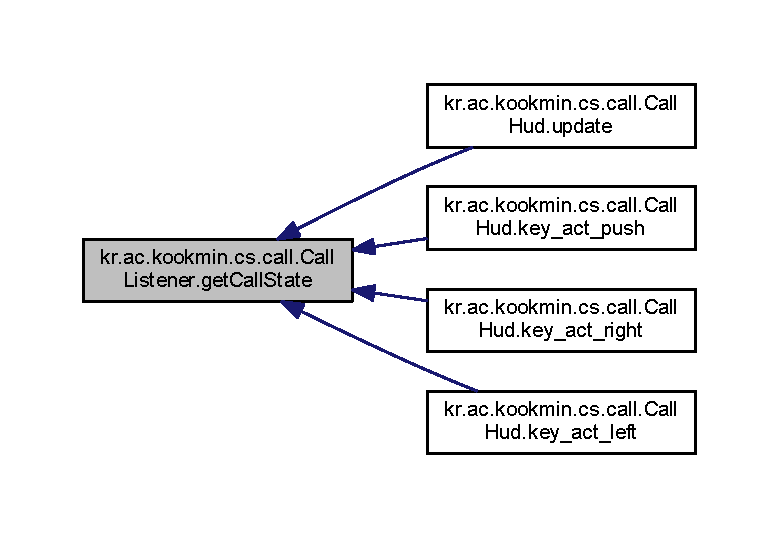
\includegraphics[width=350pt]{classkr_1_1ac_1_1kookmin_1_1cs_1_1call_1_1_call_listener_a7fceefa2570760dde2970fe8ffd8ceae_icgraph}
\end{center}
\end{figure}


\hypertarget{classkr_1_1ac_1_1kookmin_1_1cs_1_1call_1_1_call_listener_afcbd7b4289361b3d773cafa29f033f89}{}\index{kr\+::ac\+::kookmin\+::cs\+::call\+::\+Call\+Listener@{kr\+::ac\+::kookmin\+::cs\+::call\+::\+Call\+Listener}!get\+Sender@{get\+Sender}}
\index{get\+Sender@{get\+Sender}!kr\+::ac\+::kookmin\+::cs\+::call\+::\+Call\+Listener@{kr\+::ac\+::kookmin\+::cs\+::call\+::\+Call\+Listener}}
\subsubsection[{get\+Sender}]{\setlength{\rightskip}{0pt plus 5cm}static String kr.\+ac.\+kookmin.\+cs.\+call.\+Call\+Listener.\+get\+Sender (
\begin{DoxyParamCaption}
{}
\end{DoxyParamCaption}
)\hspace{0.3cm}{\ttfamily [static]}}\label{classkr_1_1ac_1_1kookmin_1_1cs_1_1call_1_1_call_listener_afcbd7b4289361b3d773cafa29f033f89}

\begin{DoxyCode}
45                                    \{
46     \textcolor{keywordflow}{return} \hyperlink{classkr_1_1ac_1_1kookmin_1_1cs_1_1call_1_1_call_listener_a87caf58642cf13014f53edb0fdcda07b}{sender};
47   \}
\end{DoxyCode}


이 함수를 호출하는 함수들에 대한 그래프입니다.\+:\nopagebreak
\begin{figure}[H]
\begin{center}
\leavevmode
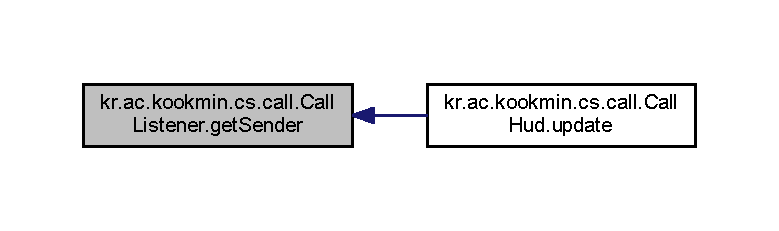
\includegraphics[width=350pt]{classkr_1_1ac_1_1kookmin_1_1cs_1_1call_1_1_call_listener_afcbd7b4289361b3d773cafa29f033f89_icgraph}
\end{center}
\end{figure}


\hypertarget{classkr_1_1ac_1_1kookmin_1_1cs_1_1call_1_1_call_listener_a886a6345c6f2ed74e64914984e270f6d}{}\index{kr\+::ac\+::kookmin\+::cs\+::call\+::\+Call\+Listener@{kr\+::ac\+::kookmin\+::cs\+::call\+::\+Call\+Listener}!is\+Call@{is\+Call}}
\index{is\+Call@{is\+Call}!kr\+::ac\+::kookmin\+::cs\+::call\+::\+Call\+Listener@{kr\+::ac\+::kookmin\+::cs\+::call\+::\+Call\+Listener}}
\subsubsection[{is\+Call}]{\setlength{\rightskip}{0pt plus 5cm}static boolean kr.\+ac.\+kookmin.\+cs.\+call.\+Call\+Listener.\+is\+Call (
\begin{DoxyParamCaption}
{}
\end{DoxyParamCaption}
)\hspace{0.3cm}{\ttfamily [static]}}\label{classkr_1_1ac_1_1kookmin_1_1cs_1_1call_1_1_call_listener_a886a6345c6f2ed74e64914984e270f6d}


Method to check whether or not the call state. 


\begin{DoxyParams}{매개변수}
{\em Nothing} & \\
\hline
\end{DoxyParams}
\begin{DoxyReturn}{반환값}
It returns true if during a call , it returns false otherwise. 
\end{DoxyReturn}

\begin{DoxyCode}
41                                 \{
42     \textcolor{keywordflow}{return} \hyperlink{classkr_1_1ac_1_1kookmin_1_1cs_1_1call_1_1_call_listener_a43a92315d34bbf897048aea788679fbc}{flag};
43   \}
\end{DoxyCode}


이 함수를 호출하는 함수들에 대한 그래프입니다.\+:\nopagebreak
\begin{figure}[H]
\begin{center}
\leavevmode
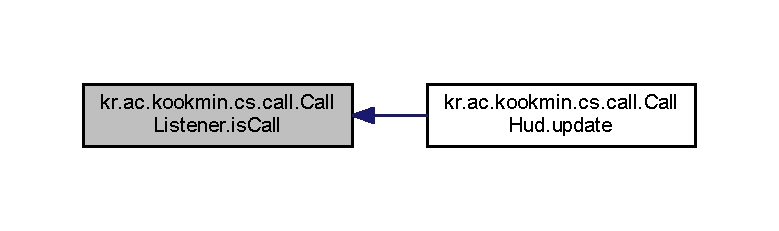
\includegraphics[width=350pt]{classkr_1_1ac_1_1kookmin_1_1cs_1_1call_1_1_call_listener_a886a6345c6f2ed74e64914984e270f6d_icgraph}
\end{center}
\end{figure}


\hypertarget{classkr_1_1ac_1_1kookmin_1_1cs_1_1call_1_1_call_listener_a2fdc9350dd23a0b6a706919b2cd2c59e}{}\index{kr\+::ac\+::kookmin\+::cs\+::call\+::\+Call\+Listener@{kr\+::ac\+::kookmin\+::cs\+::call\+::\+Call\+Listener}!on\+Call@{on\+Call}}
\index{on\+Call@{on\+Call}!kr\+::ac\+::kookmin\+::cs\+::call\+::\+Call\+Listener@{kr\+::ac\+::kookmin\+::cs\+::call\+::\+Call\+Listener}}
\subsubsection[{on\+Call}]{\setlength{\rightskip}{0pt plus 5cm}static void kr.\+ac.\+kookmin.\+cs.\+call.\+Call\+Listener.\+on\+Call (
\begin{DoxyParamCaption}
{}
\end{DoxyParamCaption}
)\hspace{0.3cm}{\ttfamily [static]}}\label{classkr_1_1ac_1_1kookmin_1_1cs_1_1call_1_1_call_listener_a2fdc9350dd23a0b6a706919b2cd2c59e}


It sends a message of receiving a phone call to the mobile in this method. 


\begin{DoxyParams}{매개변수}
{\em Nothing} & \\
\hline
\end{DoxyParams}
\begin{DoxyReturn}{반환값}
Nothing 
\end{DoxyReturn}

\begin{DoxyCode}
80                              \{
81     ProcessConnectionThread.sendData(\textcolor{stringliteral}{"onCall"});
82     \hyperlink{classkr_1_1ac_1_1kookmin_1_1cs_1_1call_1_1_call_listener_a03420a995d78c4421f4fe92b75be5647}{call\_state} = 1;
83   \}
\end{DoxyCode}


이 함수 내부에서 호출하는 함수들에 대한 그래프입니다.\+:\nopagebreak
\begin{figure}[H]
\begin{center}
\leavevmode
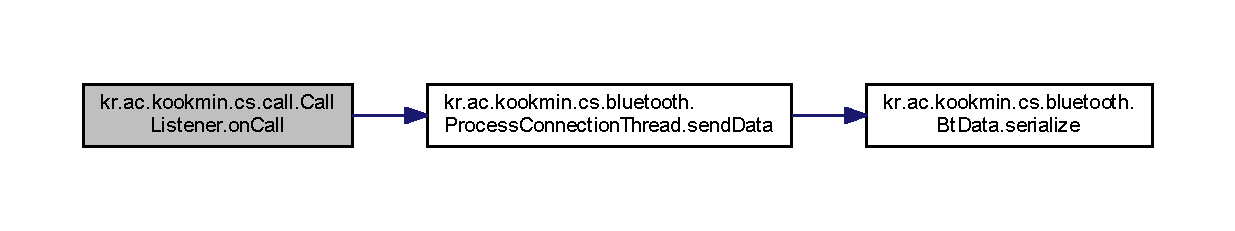
\includegraphics[width=350pt]{classkr_1_1ac_1_1kookmin_1_1cs_1_1call_1_1_call_listener_a2fdc9350dd23a0b6a706919b2cd2c59e_cgraph}
\end{center}
\end{figure}




이 함수를 호출하는 함수들에 대한 그래프입니다.\+:\nopagebreak
\begin{figure}[H]
\begin{center}
\leavevmode
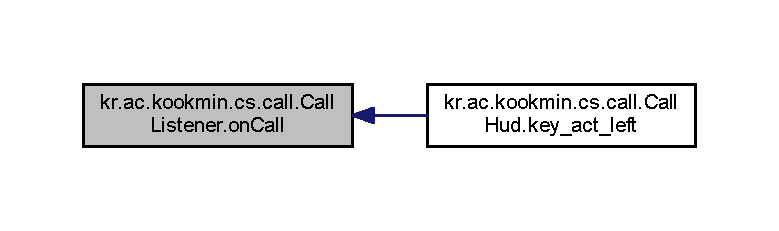
\includegraphics[width=350pt]{classkr_1_1ac_1_1kookmin_1_1cs_1_1call_1_1_call_listener_a2fdc9350dd23a0b6a706919b2cd2c59e_icgraph}
\end{center}
\end{figure}


\hypertarget{classkr_1_1ac_1_1kookmin_1_1cs_1_1call_1_1_call_listener_aec282649d8f8b5690d1bf7c5e7e73781}{}\index{kr\+::ac\+::kookmin\+::cs\+::call\+::\+Call\+Listener@{kr\+::ac\+::kookmin\+::cs\+::call\+::\+Call\+Listener}!set\+Call\+State@{set\+Call\+State}}
\index{set\+Call\+State@{set\+Call\+State}!kr\+::ac\+::kookmin\+::cs\+::call\+::\+Call\+Listener@{kr\+::ac\+::kookmin\+::cs\+::call\+::\+Call\+Listener}}
\subsubsection[{set\+Call\+State}]{\setlength{\rightskip}{0pt plus 5cm}static void kr.\+ac.\+kookmin.\+cs.\+call.\+Call\+Listener.\+set\+Call\+State (
\begin{DoxyParamCaption}
\item[{int}]{state}
\end{DoxyParamCaption}
)\hspace{0.3cm}{\ttfamily [static]}}\label{classkr_1_1ac_1_1kookmin_1_1cs_1_1call_1_1_call_listener_aec282649d8f8b5690d1bf7c5e7e73781}

\begin{DoxyCode}
32                                             \{
33     \hyperlink{classkr_1_1ac_1_1kookmin_1_1cs_1_1call_1_1_call_listener_a03420a995d78c4421f4fe92b75be5647}{call\_state} = state;
34   \}
\end{DoxyCode}


이 함수를 호출하는 함수들에 대한 그래프입니다.\+:\nopagebreak
\begin{figure}[H]
\begin{center}
\leavevmode
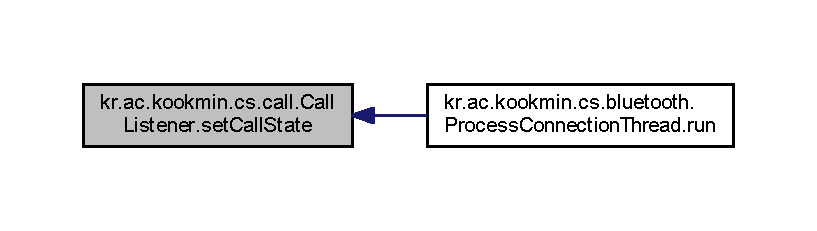
\includegraphics[width=350pt]{classkr_1_1ac_1_1kookmin_1_1cs_1_1call_1_1_call_listener_aec282649d8f8b5690d1bf7c5e7e73781_icgraph}
\end{center}
\end{figure}


\hypertarget{classkr_1_1ac_1_1kookmin_1_1cs_1_1call_1_1_call_listener_a11abb308347a972e68de7eed6b569a7b}{}\index{kr\+::ac\+::kookmin\+::cs\+::call\+::\+Call\+Listener@{kr\+::ac\+::kookmin\+::cs\+::call\+::\+Call\+Listener}!set\+End@{set\+End}}
\index{set\+End@{set\+End}!kr\+::ac\+::kookmin\+::cs\+::call\+::\+Call\+Listener@{kr\+::ac\+::kookmin\+::cs\+::call\+::\+Call\+Listener}}
\subsubsection[{set\+End}]{\setlength{\rightskip}{0pt plus 5cm}static void kr.\+ac.\+kookmin.\+cs.\+call.\+Call\+Listener.\+set\+End (
\begin{DoxyParamCaption}
{}
\end{DoxyParamCaption}
)\hspace{0.3cm}{\ttfamily [static]}}\label{classkr_1_1ac_1_1kookmin_1_1cs_1_1call_1_1_call_listener_a11abb308347a972e68de7eed6b569a7b}


It wants to change to the end state of the call. 


\begin{DoxyParams}{매개변수}
{\em Nothing} & \\
\hline
\end{DoxyParams}
\begin{DoxyReturn}{반환값}
Nothing 
\end{DoxyReturn}

\begin{DoxyCode}
59                              \{
60     \hyperlink{classkr_1_1ac_1_1kookmin_1_1cs_1_1call_1_1_call_listener_a03420a995d78c4421f4fe92b75be5647}{call\_state} = 0;
61     \hyperlink{classkr_1_1ac_1_1kookmin_1_1cs_1_1call_1_1_call_listener_a43a92315d34bbf897048aea788679fbc}{flag} = \textcolor{keyword}{false};
62   \}
\end{DoxyCode}


이 함수를 호출하는 함수들에 대한 그래프입니다.\+:\nopagebreak
\begin{figure}[H]
\begin{center}
\leavevmode
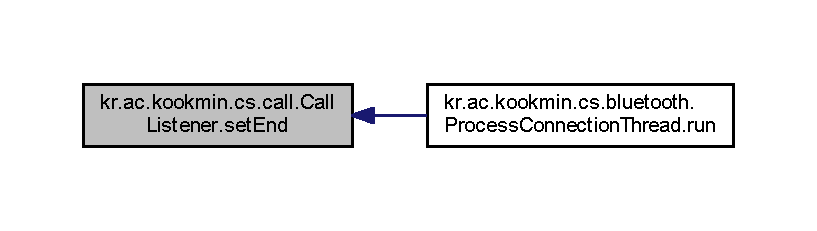
\includegraphics[width=350pt]{classkr_1_1ac_1_1kookmin_1_1cs_1_1call_1_1_call_listener_a11abb308347a972e68de7eed6b569a7b_icgraph}
\end{center}
\end{figure}


\hypertarget{classkr_1_1ac_1_1kookmin_1_1cs_1_1call_1_1_call_listener_a4a5fc9ec67f36eed4c2e934875abf007}{}\index{kr\+::ac\+::kookmin\+::cs\+::call\+::\+Call\+Listener@{kr\+::ac\+::kookmin\+::cs\+::call\+::\+Call\+Listener}!set\+Sender@{set\+Sender}}
\index{set\+Sender@{set\+Sender}!kr\+::ac\+::kookmin\+::cs\+::call\+::\+Call\+Listener@{kr\+::ac\+::kookmin\+::cs\+::call\+::\+Call\+Listener}}
\subsubsection[{set\+Sender}]{\setlength{\rightskip}{0pt plus 5cm}static void kr.\+ac.\+kookmin.\+cs.\+call.\+Call\+Listener.\+set\+Sender (
\begin{DoxyParamCaption}
\item[{String}]{sender}
\end{DoxyParamCaption}
)\hspace{0.3cm}{\ttfamily [static]}}\label{classkr_1_1ac_1_1kookmin_1_1cs_1_1call_1_1_call_listener_a4a5fc9ec67f36eed4c2e934875abf007}

\begin{DoxyCode}
49                                               \{
50     CallListener.sender = \hyperlink{classkr_1_1ac_1_1kookmin_1_1cs_1_1call_1_1_call_listener_a87caf58642cf13014f53edb0fdcda07b}{sender};
51     \hyperlink{classkr_1_1ac_1_1kookmin_1_1cs_1_1call_1_1_call_listener_a43a92315d34bbf897048aea788679fbc}{flag} = \textcolor{keyword}{true};
52   \}
\end{DoxyCode}


이 함수를 호출하는 함수들에 대한 그래프입니다.\+:\nopagebreak
\begin{figure}[H]
\begin{center}
\leavevmode
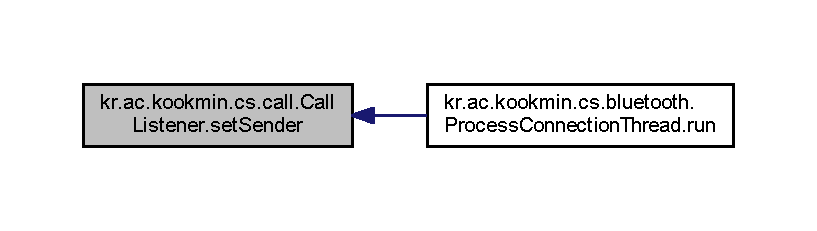
\includegraphics[width=350pt]{classkr_1_1ac_1_1kookmin_1_1cs_1_1call_1_1_call_listener_a4a5fc9ec67f36eed4c2e934875abf007_icgraph}
\end{center}
\end{figure}




\subsection{멤버 데이타 문서화}
\hypertarget{classkr_1_1ac_1_1kookmin_1_1cs_1_1call_1_1_call_listener_a03420a995d78c4421f4fe92b75be5647}{}\index{kr\+::ac\+::kookmin\+::cs\+::call\+::\+Call\+Listener@{kr\+::ac\+::kookmin\+::cs\+::call\+::\+Call\+Listener}!call\+\_\+state@{call\+\_\+state}}
\index{call\+\_\+state@{call\+\_\+state}!kr\+::ac\+::kookmin\+::cs\+::call\+::\+Call\+Listener@{kr\+::ac\+::kookmin\+::cs\+::call\+::\+Call\+Listener}}
\subsubsection[{call\+\_\+state}]{\setlength{\rightskip}{0pt plus 5cm}int kr.\+ac.\+kookmin.\+cs.\+call.\+Call\+Listener.\+call\+\_\+state = 0\hspace{0.3cm}{\ttfamily [static]}, {\ttfamily [private]}}\label{classkr_1_1ac_1_1kookmin_1_1cs_1_1call_1_1_call_listener_a03420a995d78c4421f4fe92b75be5647}
\hypertarget{classkr_1_1ac_1_1kookmin_1_1cs_1_1call_1_1_call_listener_a43a92315d34bbf897048aea788679fbc}{}\index{kr\+::ac\+::kookmin\+::cs\+::call\+::\+Call\+Listener@{kr\+::ac\+::kookmin\+::cs\+::call\+::\+Call\+Listener}!flag@{flag}}
\index{flag@{flag}!kr\+::ac\+::kookmin\+::cs\+::call\+::\+Call\+Listener@{kr\+::ac\+::kookmin\+::cs\+::call\+::\+Call\+Listener}}
\subsubsection[{flag}]{\setlength{\rightskip}{0pt plus 5cm}boolean kr.\+ac.\+kookmin.\+cs.\+call.\+Call\+Listener.\+flag = false\hspace{0.3cm}{\ttfamily [static]}, {\ttfamily [private]}}\label{classkr_1_1ac_1_1kookmin_1_1cs_1_1call_1_1_call_listener_a43a92315d34bbf897048aea788679fbc}
\hypertarget{classkr_1_1ac_1_1kookmin_1_1cs_1_1call_1_1_call_listener_a87caf58642cf13014f53edb0fdcda07b}{}\index{kr\+::ac\+::kookmin\+::cs\+::call\+::\+Call\+Listener@{kr\+::ac\+::kookmin\+::cs\+::call\+::\+Call\+Listener}!sender@{sender}}
\index{sender@{sender}!kr\+::ac\+::kookmin\+::cs\+::call\+::\+Call\+Listener@{kr\+::ac\+::kookmin\+::cs\+::call\+::\+Call\+Listener}}
\subsubsection[{sender}]{\setlength{\rightskip}{0pt plus 5cm}String kr.\+ac.\+kookmin.\+cs.\+call.\+Call\+Listener.\+sender = \char`\"{}\char`\"{}\hspace{0.3cm}{\ttfamily [static]}, {\ttfamily [private]}}\label{classkr_1_1ac_1_1kookmin_1_1cs_1_1call_1_1_call_listener_a87caf58642cf13014f53edb0fdcda07b}


이 클래스에 대한 문서화 페이지는 다음의 파일로부터 생성되었습니다.\+:\begin{DoxyCompactItemize}
\item 
C\+:/\+Users/\+Karasion/git/\+Capstone2015-\/\+Purple\+Ocean/src/kr/ac/kookmin/cs/call/\hyperlink{_call_listener_8java}{Call\+Listener.\+java}\end{DoxyCompactItemize}

\hypertarget{classkr_1_1ac_1_1kookmin_1_1cs_1_1hud_1_1_h_u_d_class_template}{}\section{kr.\+ac.\+kookmin.\+cs.\+hud.\+H\+U\+D\+Class\+Template 클래스 참조}
\label{classkr_1_1ac_1_1kookmin_1_1cs_1_1hud_1_1_h_u_d_class_template}\index{kr.\+ac.\+kookmin.\+cs.\+hud.\+H\+U\+D\+Class\+Template@{kr.\+ac.\+kookmin.\+cs.\+hud.\+H\+U\+D\+Class\+Template}}


This class stub is a template for the H\+U\+D layout class.  




kr.\+ac.\+kookmin.\+cs.\+hud.\+H\+U\+D\+Class\+Template에 대한 상속 다이어그램 \+: \nopagebreak
\begin{figure}[H]
\begin{center}
\leavevmode
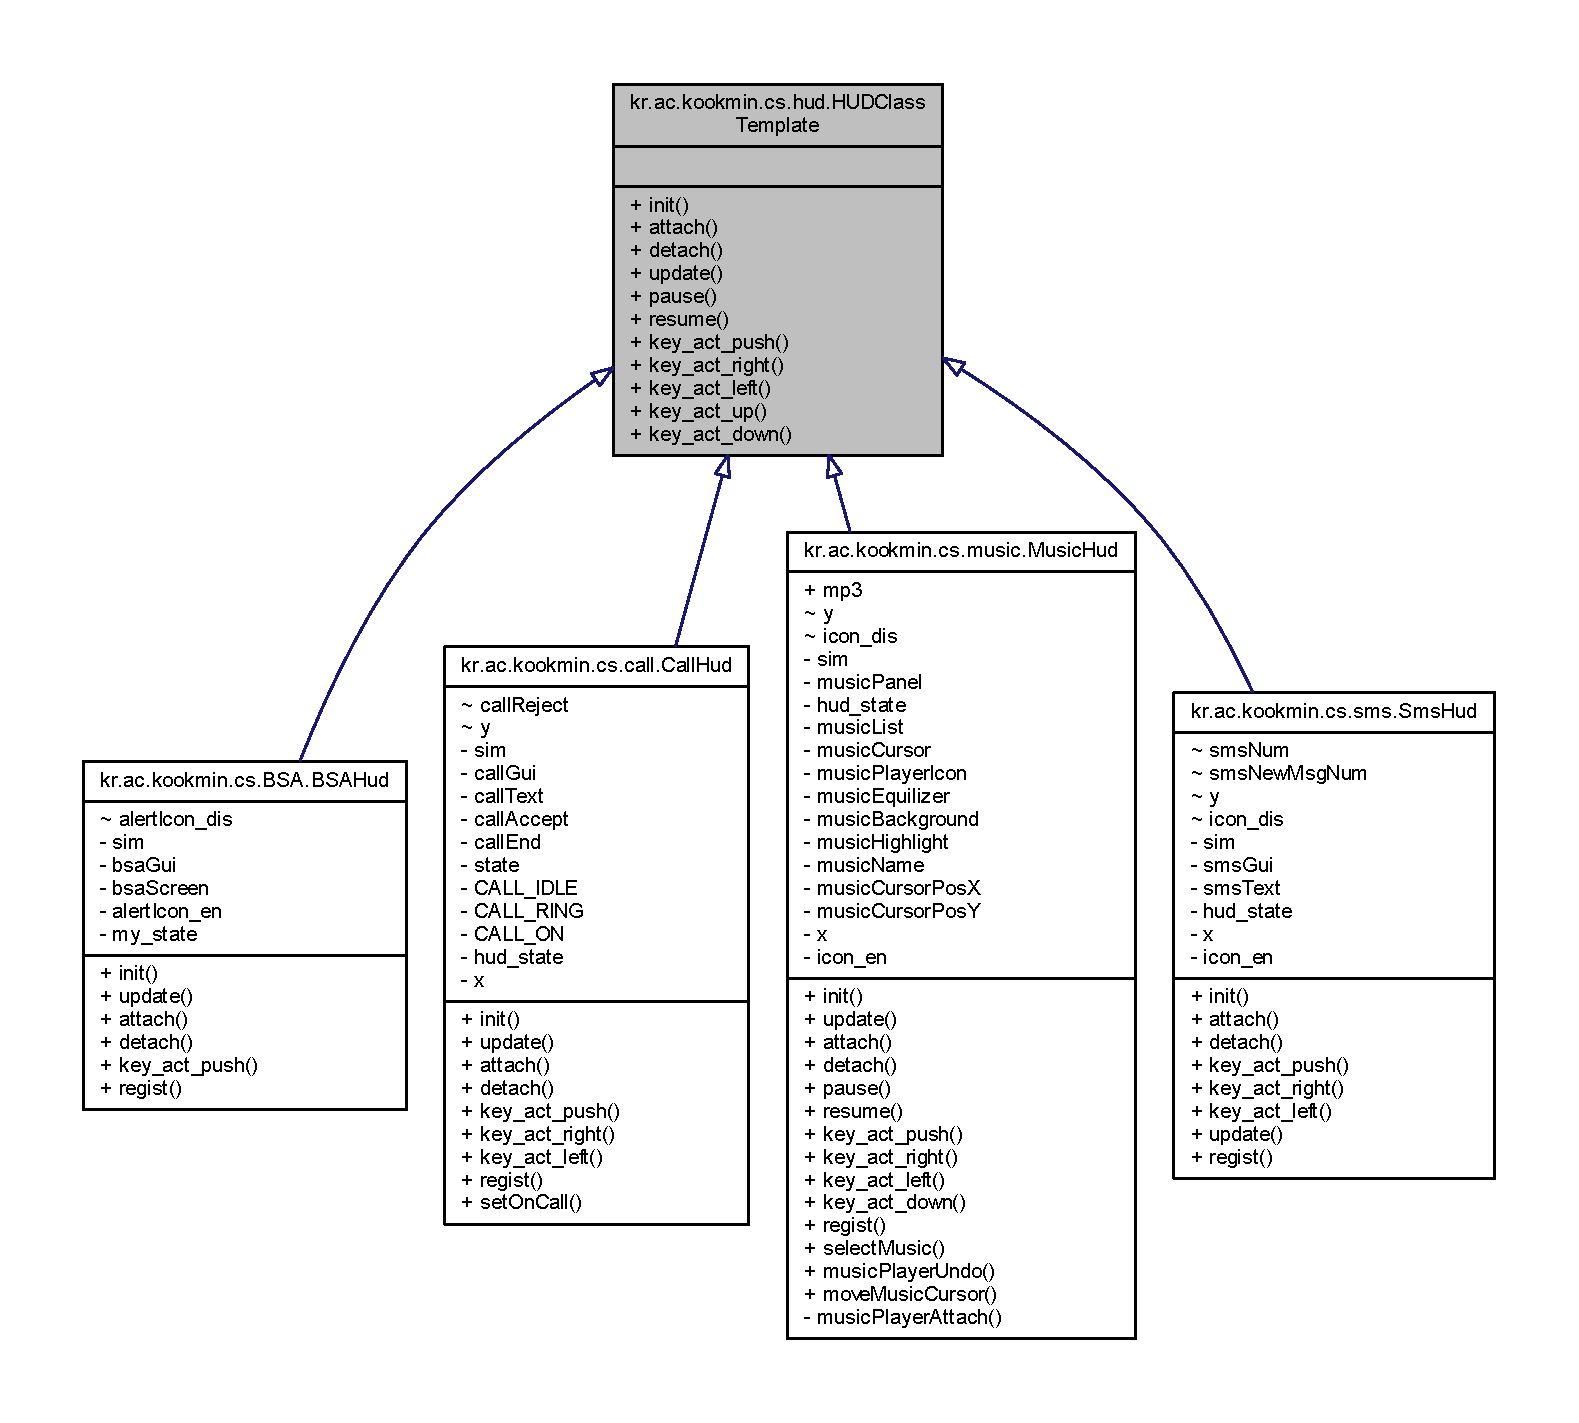
\includegraphics[width=350pt]{classkr_1_1ac_1_1kookmin_1_1cs_1_1hud_1_1_h_u_d_class_template__inherit__graph}
\end{center}
\end{figure}


kr.\+ac.\+kookmin.\+cs.\+hud.\+H\+U\+D\+Class\+Template에 대한 협력 다이어그램\+:\nopagebreak
\begin{figure}[H]
\begin{center}
\leavevmode
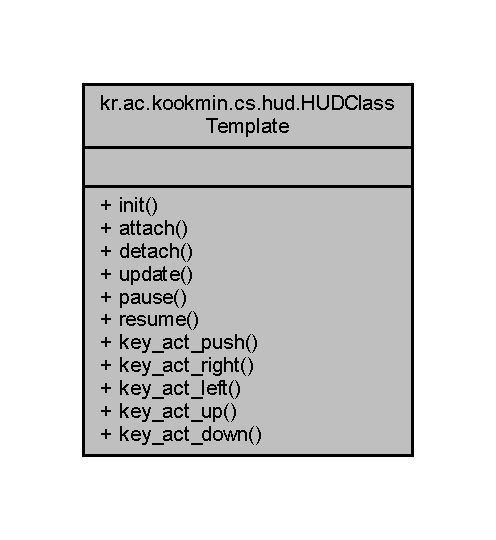
\includegraphics[width=238pt]{classkr_1_1ac_1_1kookmin_1_1cs_1_1hud_1_1_h_u_d_class_template__coll__graph}
\end{center}
\end{figure}
\subsection*{Public 멤버 함수}
\begin{DoxyCompactItemize}
\item 
abstract void \hyperlink{classkr_1_1ac_1_1kookmin_1_1cs_1_1hud_1_1_h_u_d_class_template_a30a209182edaf92713b172109e0e4693}{init} (Simulator simulator)
\begin{DoxyCompactList}\small\item\em You must initialize the elements of layout in this method. And you must also add a menu bar icon . \end{DoxyCompactList}\item 
abstract void \hyperlink{classkr_1_1ac_1_1kookmin_1_1cs_1_1hud_1_1_h_u_d_class_template_a053bfe4a8c5121e8910f1c6416e3da4c}{attach} ()
\begin{DoxyCompactList}\small\item\em Inside this method it is necessary to implement the tasks required when H\+U\+D layout inserted. \end{DoxyCompactList}\item 
abstract void \hyperlink{classkr_1_1ac_1_1kookmin_1_1cs_1_1hud_1_1_h_u_d_class_template_a24cbcfc7dac21b475f806b9298b9846e}{detach} ()
\begin{DoxyCompactList}\small\item\em Inside this method it is necessary to implement the tasks required when H\+U\+D layout deleted. \end{DoxyCompactList}\item 
abstract void \hyperlink{classkr_1_1ac_1_1kookmin_1_1cs_1_1hud_1_1_h_u_d_class_template_aa50760c142875775a12df392814f4572}{update} ()
\begin{DoxyCompactList}\small\item\em This method to implement the layout change . \end{DoxyCompactList}\item 
void \hyperlink{classkr_1_1ac_1_1kookmin_1_1cs_1_1hud_1_1_h_u_d_class_template_abb46b8cd2704ee02c1de01b8e60bae62}{pause} ()
\begin{DoxyCompactList}\small\item\em This metho to implement what you need in the application that H\+U\+D is paused. \end{DoxyCompactList}\item 
void \hyperlink{classkr_1_1ac_1_1kookmin_1_1cs_1_1hud_1_1_h_u_d_class_template_ae546a0f18829e5012b1f0ae1c82ee4bb}{resume} ()
\begin{DoxyCompactList}\small\item\em This metho to implement what you need in the application that H\+U\+D is resumed . \end{DoxyCompactList}\item 
void \hyperlink{classkr_1_1ac_1_1kookmin_1_1cs_1_1hud_1_1_h_u_d_class_template_a030e54909c369e4b0e43b551561e238d}{key\+\_\+act\+\_\+push} ()
\begin{DoxyCompactList}\small\item\em This metho to implement the action of push key. \end{DoxyCompactList}\item 
void \hyperlink{classkr_1_1ac_1_1kookmin_1_1cs_1_1hud_1_1_h_u_d_class_template_affc56ae2354935530ed2bd0c580d32f0}{key\+\_\+act\+\_\+right} ()
\begin{DoxyCompactList}\small\item\em This metho to implement the action of right key. \end{DoxyCompactList}\item 
void \hyperlink{classkr_1_1ac_1_1kookmin_1_1cs_1_1hud_1_1_h_u_d_class_template_a475ddeb053862cfd976e4a5a1548340e}{key\+\_\+act\+\_\+left} ()
\begin{DoxyCompactList}\small\item\em This metho to implement the action of left key. \end{DoxyCompactList}\item 
void \hyperlink{classkr_1_1ac_1_1kookmin_1_1cs_1_1hud_1_1_h_u_d_class_template_a6997c3296b9aa23172090ba4c03b0604}{key\+\_\+act\+\_\+up} ()
\begin{DoxyCompactList}\small\item\em This metho to implement the action of up key. \end{DoxyCompactList}\item 
void \hyperlink{classkr_1_1ac_1_1kookmin_1_1cs_1_1hud_1_1_h_u_d_class_template_a56b533f34b6b984287388a344e732e00}{key\+\_\+act\+\_\+down} ()
\begin{DoxyCompactList}\small\item\em This metho to implement the action of down key. \end{DoxyCompactList}\end{DoxyCompactItemize}


\subsection{상세한 설명}
This class stub is a template for the H\+U\+D layout class. 

All H\+U\+D layout class must inherit this class. And some method must always be implemented. \begin{DoxyAuthor}{작성자}
Jo-\/kwanghyeon 
\end{DoxyAuthor}


\subsection{멤버 함수 문서화}
\hypertarget{classkr_1_1ac_1_1kookmin_1_1cs_1_1hud_1_1_h_u_d_class_template_a053bfe4a8c5121e8910f1c6416e3da4c}{}\index{kr\+::ac\+::kookmin\+::cs\+::hud\+::\+H\+U\+D\+Class\+Template@{kr\+::ac\+::kookmin\+::cs\+::hud\+::\+H\+U\+D\+Class\+Template}!attach@{attach}}
\index{attach@{attach}!kr\+::ac\+::kookmin\+::cs\+::hud\+::\+H\+U\+D\+Class\+Template@{kr\+::ac\+::kookmin\+::cs\+::hud\+::\+H\+U\+D\+Class\+Template}}
\subsubsection[{attach}]{\setlength{\rightskip}{0pt plus 5cm}abstract void kr.\+ac.\+kookmin.\+cs.\+hud.\+H\+U\+D\+Class\+Template.\+attach (
\begin{DoxyParamCaption}
{}
\end{DoxyParamCaption}
)\hspace{0.3cm}{\ttfamily [abstract]}}\label{classkr_1_1ac_1_1kookmin_1_1cs_1_1hud_1_1_h_u_d_class_template_a053bfe4a8c5121e8910f1c6416e3da4c}


Inside this method it is necessary to implement the tasks required when H\+U\+D layout inserted. 


\begin{DoxyParams}{매개변수}
{\em Nothing} & \\
\hline
\end{DoxyParams}
\begin{DoxyReturn}{반환값}
Nothing 
\end{DoxyReturn}
\hypertarget{classkr_1_1ac_1_1kookmin_1_1cs_1_1hud_1_1_h_u_d_class_template_a24cbcfc7dac21b475f806b9298b9846e}{}\index{kr\+::ac\+::kookmin\+::cs\+::hud\+::\+H\+U\+D\+Class\+Template@{kr\+::ac\+::kookmin\+::cs\+::hud\+::\+H\+U\+D\+Class\+Template}!detach@{detach}}
\index{detach@{detach}!kr\+::ac\+::kookmin\+::cs\+::hud\+::\+H\+U\+D\+Class\+Template@{kr\+::ac\+::kookmin\+::cs\+::hud\+::\+H\+U\+D\+Class\+Template}}
\subsubsection[{detach}]{\setlength{\rightskip}{0pt plus 5cm}abstract void kr.\+ac.\+kookmin.\+cs.\+hud.\+H\+U\+D\+Class\+Template.\+detach (
\begin{DoxyParamCaption}
{}
\end{DoxyParamCaption}
)\hspace{0.3cm}{\ttfamily [abstract]}}\label{classkr_1_1ac_1_1kookmin_1_1cs_1_1hud_1_1_h_u_d_class_template_a24cbcfc7dac21b475f806b9298b9846e}


Inside this method it is necessary to implement the tasks required when H\+U\+D layout deleted. 


\begin{DoxyParams}{매개변수}
{\em Nothing} & \\
\hline
\end{DoxyParams}
\begin{DoxyReturn}{반환값}
Nothing 
\end{DoxyReturn}
\hypertarget{classkr_1_1ac_1_1kookmin_1_1cs_1_1hud_1_1_h_u_d_class_template_a30a209182edaf92713b172109e0e4693}{}\index{kr\+::ac\+::kookmin\+::cs\+::hud\+::\+H\+U\+D\+Class\+Template@{kr\+::ac\+::kookmin\+::cs\+::hud\+::\+H\+U\+D\+Class\+Template}!init@{init}}
\index{init@{init}!kr\+::ac\+::kookmin\+::cs\+::hud\+::\+H\+U\+D\+Class\+Template@{kr\+::ac\+::kookmin\+::cs\+::hud\+::\+H\+U\+D\+Class\+Template}}
\subsubsection[{init}]{\setlength{\rightskip}{0pt plus 5cm}abstract void kr.\+ac.\+kookmin.\+cs.\+hud.\+H\+U\+D\+Class\+Template.\+init (
\begin{DoxyParamCaption}
\item[{Simulator}]{simulator}
\end{DoxyParamCaption}
)\hspace{0.3cm}{\ttfamily [abstract]}}\label{classkr_1_1ac_1_1kookmin_1_1cs_1_1hud_1_1_h_u_d_class_template_a30a209182edaf92713b172109e0e4693}


You must initialize the elements of layout in this method. And you must also add a menu bar icon . 


\begin{DoxyParams}{매개변수}
{\em Simulator} & argument simulator. This is used to utilize the A\+P\+I in Jme3. \\
\hline
\end{DoxyParams}
\begin{DoxyReturn}{반환값}
Nothing 
\end{DoxyReturn}
\hypertarget{classkr_1_1ac_1_1kookmin_1_1cs_1_1hud_1_1_h_u_d_class_template_a56b533f34b6b984287388a344e732e00}{}\index{kr\+::ac\+::kookmin\+::cs\+::hud\+::\+H\+U\+D\+Class\+Template@{kr\+::ac\+::kookmin\+::cs\+::hud\+::\+H\+U\+D\+Class\+Template}!key\+\_\+act\+\_\+down@{key\+\_\+act\+\_\+down}}
\index{key\+\_\+act\+\_\+down@{key\+\_\+act\+\_\+down}!kr\+::ac\+::kookmin\+::cs\+::hud\+::\+H\+U\+D\+Class\+Template@{kr\+::ac\+::kookmin\+::cs\+::hud\+::\+H\+U\+D\+Class\+Template}}
\subsubsection[{key\+\_\+act\+\_\+down}]{\setlength{\rightskip}{0pt plus 5cm}void kr.\+ac.\+kookmin.\+cs.\+hud.\+H\+U\+D\+Class\+Template.\+key\+\_\+act\+\_\+down (
\begin{DoxyParamCaption}
{}
\end{DoxyParamCaption}
)}\label{classkr_1_1ac_1_1kookmin_1_1cs_1_1hud_1_1_h_u_d_class_template_a56b533f34b6b984287388a344e732e00}


This metho to implement the action of down key. 


\begin{DoxyParams}{매개변수}
{\em Nothing} & \\
\hline
\end{DoxyParams}
\begin{DoxyReturn}{반환값}
Nothing 
\end{DoxyReturn}

\begin{DoxyCode}
104   \{
105   \}
\end{DoxyCode}
\hypertarget{classkr_1_1ac_1_1kookmin_1_1cs_1_1hud_1_1_h_u_d_class_template_a475ddeb053862cfd976e4a5a1548340e}{}\index{kr\+::ac\+::kookmin\+::cs\+::hud\+::\+H\+U\+D\+Class\+Template@{kr\+::ac\+::kookmin\+::cs\+::hud\+::\+H\+U\+D\+Class\+Template}!key\+\_\+act\+\_\+left@{key\+\_\+act\+\_\+left}}
\index{key\+\_\+act\+\_\+left@{key\+\_\+act\+\_\+left}!kr\+::ac\+::kookmin\+::cs\+::hud\+::\+H\+U\+D\+Class\+Template@{kr\+::ac\+::kookmin\+::cs\+::hud\+::\+H\+U\+D\+Class\+Template}}
\subsubsection[{key\+\_\+act\+\_\+left}]{\setlength{\rightskip}{0pt plus 5cm}void kr.\+ac.\+kookmin.\+cs.\+hud.\+H\+U\+D\+Class\+Template.\+key\+\_\+act\+\_\+left (
\begin{DoxyParamCaption}
{}
\end{DoxyParamCaption}
)}\label{classkr_1_1ac_1_1kookmin_1_1cs_1_1hud_1_1_h_u_d_class_template_a475ddeb053862cfd976e4a5a1548340e}


This metho to implement the action of left key. 


\begin{DoxyParams}{매개변수}
{\em Nothing} & \\
\hline
\end{DoxyParams}
\begin{DoxyReturn}{반환값}
Nothing 
\end{DoxyReturn}

\begin{DoxyCode}
88   \{
89   \}
\end{DoxyCode}
\hypertarget{classkr_1_1ac_1_1kookmin_1_1cs_1_1hud_1_1_h_u_d_class_template_a030e54909c369e4b0e43b551561e238d}{}\index{kr\+::ac\+::kookmin\+::cs\+::hud\+::\+H\+U\+D\+Class\+Template@{kr\+::ac\+::kookmin\+::cs\+::hud\+::\+H\+U\+D\+Class\+Template}!key\+\_\+act\+\_\+push@{key\+\_\+act\+\_\+push}}
\index{key\+\_\+act\+\_\+push@{key\+\_\+act\+\_\+push}!kr\+::ac\+::kookmin\+::cs\+::hud\+::\+H\+U\+D\+Class\+Template@{kr\+::ac\+::kookmin\+::cs\+::hud\+::\+H\+U\+D\+Class\+Template}}
\subsubsection[{key\+\_\+act\+\_\+push}]{\setlength{\rightskip}{0pt plus 5cm}void kr.\+ac.\+kookmin.\+cs.\+hud.\+H\+U\+D\+Class\+Template.\+key\+\_\+act\+\_\+push (
\begin{DoxyParamCaption}
{}
\end{DoxyParamCaption}
)}\label{classkr_1_1ac_1_1kookmin_1_1cs_1_1hud_1_1_h_u_d_class_template_a030e54909c369e4b0e43b551561e238d}


This metho to implement the action of push key. 


\begin{DoxyParams}{매개변수}
{\em Nothing} & \\
\hline
\end{DoxyParams}
\begin{DoxyReturn}{반환값}
Nothing 
\end{DoxyReturn}

\begin{DoxyCode}
72   \{
73   \}
\end{DoxyCode}
\hypertarget{classkr_1_1ac_1_1kookmin_1_1cs_1_1hud_1_1_h_u_d_class_template_affc56ae2354935530ed2bd0c580d32f0}{}\index{kr\+::ac\+::kookmin\+::cs\+::hud\+::\+H\+U\+D\+Class\+Template@{kr\+::ac\+::kookmin\+::cs\+::hud\+::\+H\+U\+D\+Class\+Template}!key\+\_\+act\+\_\+right@{key\+\_\+act\+\_\+right}}
\index{key\+\_\+act\+\_\+right@{key\+\_\+act\+\_\+right}!kr\+::ac\+::kookmin\+::cs\+::hud\+::\+H\+U\+D\+Class\+Template@{kr\+::ac\+::kookmin\+::cs\+::hud\+::\+H\+U\+D\+Class\+Template}}
\subsubsection[{key\+\_\+act\+\_\+right}]{\setlength{\rightskip}{0pt plus 5cm}void kr.\+ac.\+kookmin.\+cs.\+hud.\+H\+U\+D\+Class\+Template.\+key\+\_\+act\+\_\+right (
\begin{DoxyParamCaption}
{}
\end{DoxyParamCaption}
)}\label{classkr_1_1ac_1_1kookmin_1_1cs_1_1hud_1_1_h_u_d_class_template_affc56ae2354935530ed2bd0c580d32f0}


This metho to implement the action of right key. 


\begin{DoxyParams}{매개변수}
{\em Nothing} & \\
\hline
\end{DoxyParams}
\begin{DoxyReturn}{반환값}
Nothing 
\end{DoxyReturn}

\begin{DoxyCode}
80   \{
81   \}
\end{DoxyCode}
\hypertarget{classkr_1_1ac_1_1kookmin_1_1cs_1_1hud_1_1_h_u_d_class_template_a6997c3296b9aa23172090ba4c03b0604}{}\index{kr\+::ac\+::kookmin\+::cs\+::hud\+::\+H\+U\+D\+Class\+Template@{kr\+::ac\+::kookmin\+::cs\+::hud\+::\+H\+U\+D\+Class\+Template}!key\+\_\+act\+\_\+up@{key\+\_\+act\+\_\+up}}
\index{key\+\_\+act\+\_\+up@{key\+\_\+act\+\_\+up}!kr\+::ac\+::kookmin\+::cs\+::hud\+::\+H\+U\+D\+Class\+Template@{kr\+::ac\+::kookmin\+::cs\+::hud\+::\+H\+U\+D\+Class\+Template}}
\subsubsection[{key\+\_\+act\+\_\+up}]{\setlength{\rightskip}{0pt plus 5cm}void kr.\+ac.\+kookmin.\+cs.\+hud.\+H\+U\+D\+Class\+Template.\+key\+\_\+act\+\_\+up (
\begin{DoxyParamCaption}
{}
\end{DoxyParamCaption}
)}\label{classkr_1_1ac_1_1kookmin_1_1cs_1_1hud_1_1_h_u_d_class_template_a6997c3296b9aa23172090ba4c03b0604}


This metho to implement the action of up key. 


\begin{DoxyParams}{매개변수}
{\em Nothing} & \\
\hline
\end{DoxyParams}
\begin{DoxyReturn}{반환값}
Nothing 
\end{DoxyReturn}

\begin{DoxyCode}
96   \{
97   \}
\end{DoxyCode}
\hypertarget{classkr_1_1ac_1_1kookmin_1_1cs_1_1hud_1_1_h_u_d_class_template_abb46b8cd2704ee02c1de01b8e60bae62}{}\index{kr\+::ac\+::kookmin\+::cs\+::hud\+::\+H\+U\+D\+Class\+Template@{kr\+::ac\+::kookmin\+::cs\+::hud\+::\+H\+U\+D\+Class\+Template}!pause@{pause}}
\index{pause@{pause}!kr\+::ac\+::kookmin\+::cs\+::hud\+::\+H\+U\+D\+Class\+Template@{kr\+::ac\+::kookmin\+::cs\+::hud\+::\+H\+U\+D\+Class\+Template}}
\subsubsection[{pause}]{\setlength{\rightskip}{0pt plus 5cm}void kr.\+ac.\+kookmin.\+cs.\+hud.\+H\+U\+D\+Class\+Template.\+pause (
\begin{DoxyParamCaption}
{}
\end{DoxyParamCaption}
)}\label{classkr_1_1ac_1_1kookmin_1_1cs_1_1hud_1_1_h_u_d_class_template_abb46b8cd2704ee02c1de01b8e60bae62}


This metho to implement what you need in the application that H\+U\+D is paused. 


\begin{DoxyParams}{매개변수}
{\em Nothing} & \\
\hline
\end{DoxyParams}
\begin{DoxyReturn}{반환값}
Nothing 
\end{DoxyReturn}

\begin{DoxyCode}
56   \{
57   \}
\end{DoxyCode}
\hypertarget{classkr_1_1ac_1_1kookmin_1_1cs_1_1hud_1_1_h_u_d_class_template_ae546a0f18829e5012b1f0ae1c82ee4bb}{}\index{kr\+::ac\+::kookmin\+::cs\+::hud\+::\+H\+U\+D\+Class\+Template@{kr\+::ac\+::kookmin\+::cs\+::hud\+::\+H\+U\+D\+Class\+Template}!resume@{resume}}
\index{resume@{resume}!kr\+::ac\+::kookmin\+::cs\+::hud\+::\+H\+U\+D\+Class\+Template@{kr\+::ac\+::kookmin\+::cs\+::hud\+::\+H\+U\+D\+Class\+Template}}
\subsubsection[{resume}]{\setlength{\rightskip}{0pt plus 5cm}void kr.\+ac.\+kookmin.\+cs.\+hud.\+H\+U\+D\+Class\+Template.\+resume (
\begin{DoxyParamCaption}
{}
\end{DoxyParamCaption}
)}\label{classkr_1_1ac_1_1kookmin_1_1cs_1_1hud_1_1_h_u_d_class_template_ae546a0f18829e5012b1f0ae1c82ee4bb}


This metho to implement what you need in the application that H\+U\+D is resumed . 


\begin{DoxyParams}{매개변수}
{\em Nothing} & \\
\hline
\end{DoxyParams}
\begin{DoxyReturn}{반환값}
Nothing 
\end{DoxyReturn}

\begin{DoxyCode}
64   \{
65   \}
\end{DoxyCode}
\hypertarget{classkr_1_1ac_1_1kookmin_1_1cs_1_1hud_1_1_h_u_d_class_template_aa50760c142875775a12df392814f4572}{}\index{kr\+::ac\+::kookmin\+::cs\+::hud\+::\+H\+U\+D\+Class\+Template@{kr\+::ac\+::kookmin\+::cs\+::hud\+::\+H\+U\+D\+Class\+Template}!update@{update}}
\index{update@{update}!kr\+::ac\+::kookmin\+::cs\+::hud\+::\+H\+U\+D\+Class\+Template@{kr\+::ac\+::kookmin\+::cs\+::hud\+::\+H\+U\+D\+Class\+Template}}
\subsubsection[{update}]{\setlength{\rightskip}{0pt plus 5cm}abstract void kr.\+ac.\+kookmin.\+cs.\+hud.\+H\+U\+D\+Class\+Template.\+update (
\begin{DoxyParamCaption}
{}
\end{DoxyParamCaption}
)\hspace{0.3cm}{\ttfamily [abstract]}}\label{classkr_1_1ac_1_1kookmin_1_1cs_1_1hud_1_1_h_u_d_class_template_aa50760c142875775a12df392814f4572}


This method to implement the layout change . 


\begin{DoxyParams}{매개변수}
{\em Nothing} & \\
\hline
\end{DoxyParams}
\begin{DoxyReturn}{반환값}
Nothing 
\end{DoxyReturn}


이 클래스에 대한 문서화 페이지는 다음의 파일로부터 생성되었습니다.\+:\begin{DoxyCompactItemize}
\item 
C\+:/\+Users/\+Karasion/git/\+Capstone2015-\/\+Purple\+Ocean/src/kr/ac/kookmin/cs/hud/\hyperlink{_h_u_d_class_template_8java}{H\+U\+D\+Class\+Template.\+java}\end{DoxyCompactItemize}

\hypertarget{classkr_1_1ac_1_1kookmin_1_1cs_1_1tool_1_1_hud_layout_tool}{}\section{kr.\+ac.\+kookmin.\+cs.\+tool.\+Hud\+Layout\+Tool 클래스 참조}
\label{classkr_1_1ac_1_1kookmin_1_1cs_1_1tool_1_1_hud_layout_tool}\index{kr.\+ac.\+kookmin.\+cs.\+tool.\+Hud\+Layout\+Tool@{kr.\+ac.\+kookmin.\+cs.\+tool.\+Hud\+Layout\+Tool}}


It is a Hud element tool to try to convenient placement of .  




kr.\+ac.\+kookmin.\+cs.\+tool.\+Hud\+Layout\+Tool에 대한 협력 다이어그램\+:\nopagebreak
\begin{figure}[H]
\begin{center}
\leavevmode
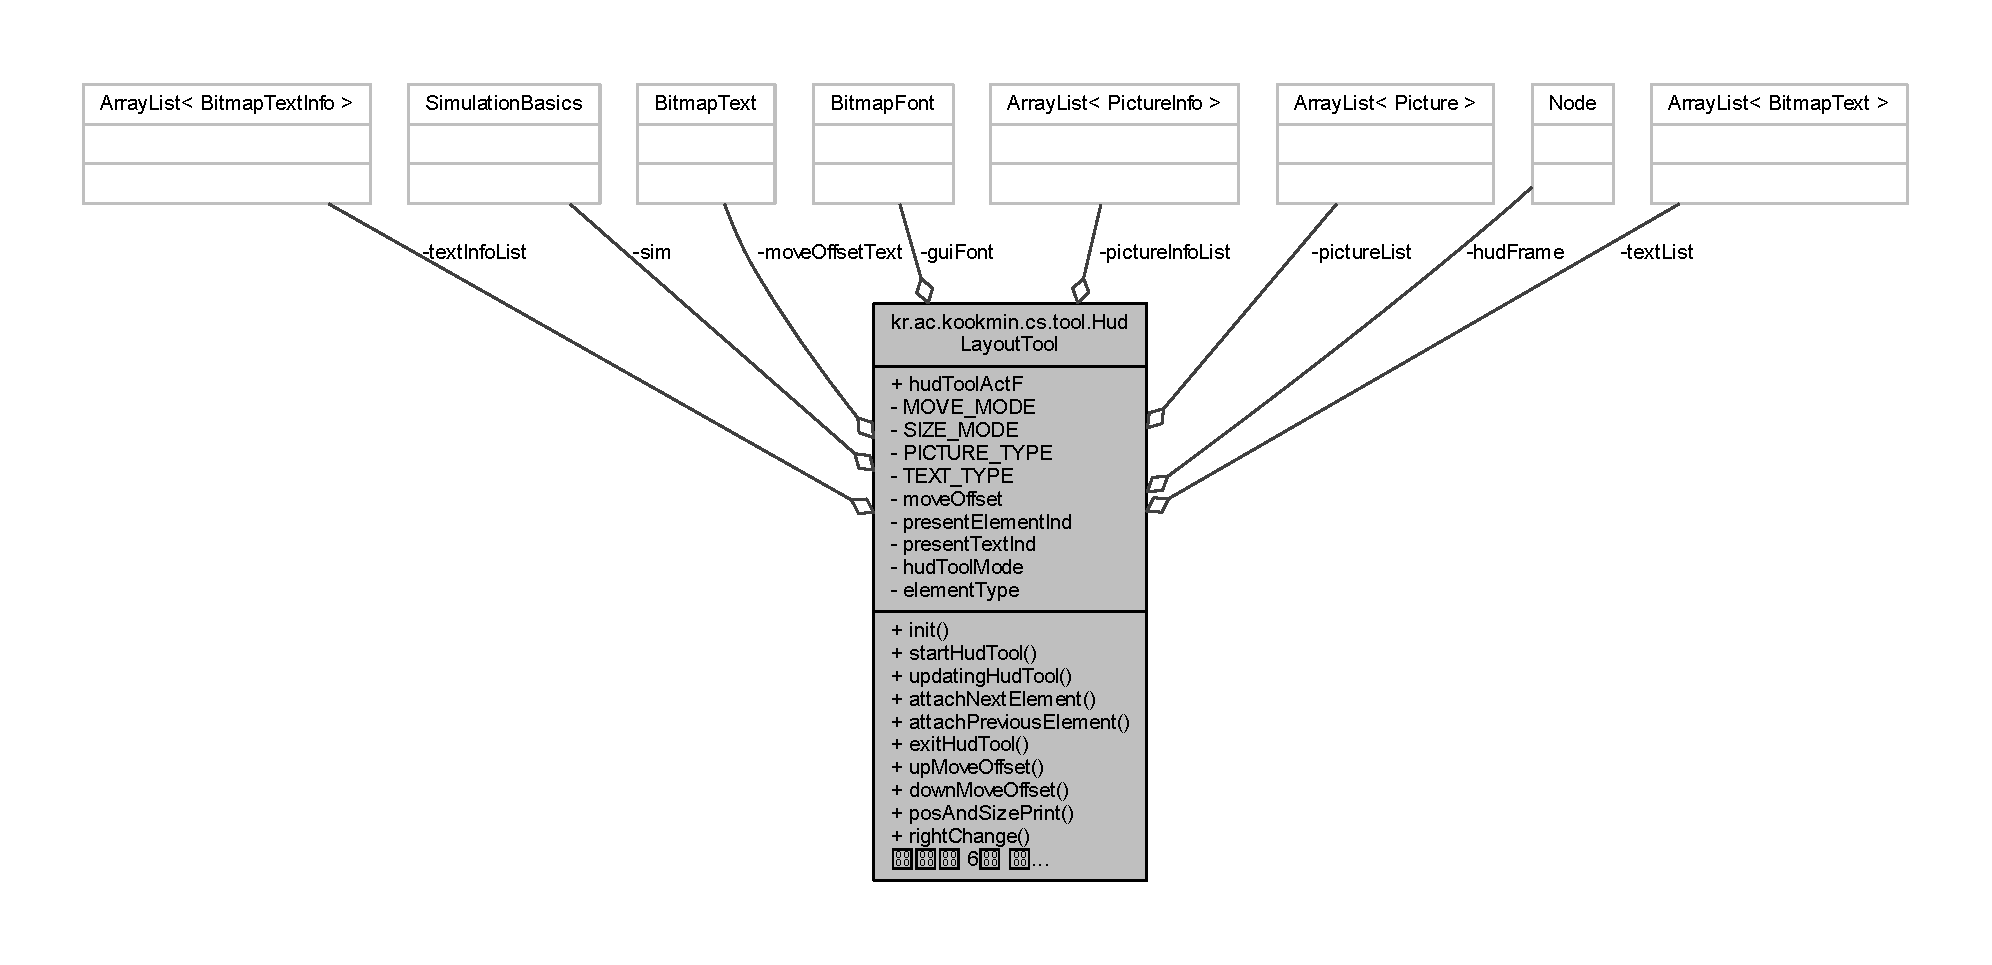
\includegraphics[width=350pt]{classkr_1_1ac_1_1kookmin_1_1cs_1_1tool_1_1_hud_layout_tool__coll__graph}
\end{center}
\end{figure}
\subsection*{클래스}
\begin{DoxyCompactItemize}
\item 
class {\bfseries Bitmap\+Text\+Info}
\begin{DoxyCompactList}\small\item\em This class has information about the elements of Bitmap\+Text. \end{DoxyCompactList}\item 
class {\bfseries Picture\+Info}
\begin{DoxyCompactList}\small\item\em This class has information about the elements of Picture. \end{DoxyCompactList}\end{DoxyCompactItemize}
\subsection*{정적 Public 멤버 함수}
\begin{DoxyCompactItemize}
\item 
static void \hyperlink{classkr_1_1ac_1_1kookmin_1_1cs_1_1tool_1_1_hud_layout_tool_a93ebf652629e4e65a6126d478143630b}{init} (Simulator simulator)
\begin{DoxyCompactList}\small\item\em This method , to set the elements for using the tool. \end{DoxyCompactList}\item 
static void \hyperlink{classkr_1_1ac_1_1kookmin_1_1cs_1_1tool_1_1_hud_layout_tool_a6f5f4dcaf3b5aeee139ab80fb3aa30aa}{start\+Hud\+Tool} ()
\begin{DoxyCompactList}\small\item\em This method is executed the \hyperlink{classkr_1_1ac_1_1kookmin_1_1cs_1_1tool_1_1_hud_layout_tool}{Hud\+Layout\+Tool} mode at startup . \end{DoxyCompactList}\item 
static void \hyperlink{classkr_1_1ac_1_1kookmin_1_1cs_1_1tool_1_1_hud_layout_tool_a1206c4b2c371bbbe24cf257492826574}{updating\+Hud\+Tool} ()
\begin{DoxyCompactList}\small\item\em Is a method to be executed in real time on the simulator . \end{DoxyCompactList}\item 
static void \hyperlink{classkr_1_1ac_1_1kookmin_1_1cs_1_1tool_1_1_hud_layout_tool_a2105ce4edf93ec4dea92c388b98f7941}{attach\+Next\+Element} ()
\begin{DoxyCompactList}\small\item\em Paste the next elements to the simulator screen . \end{DoxyCompactList}\item 
static void \hyperlink{classkr_1_1ac_1_1kookmin_1_1cs_1_1tool_1_1_hud_layout_tool_a5d9309d71fd9b0af0e6505d079bf7897}{attach\+Previous\+Element} ()
\begin{DoxyCompactList}\small\item\em Paste the previous elements to the simulator screen . \end{DoxyCompactList}\item 
static void \hyperlink{classkr_1_1ac_1_1kookmin_1_1cs_1_1tool_1_1_hud_layout_tool_aa05a256bff284acae80d81b6eb3da383}{exit\+Hud\+Tool} ()
\begin{DoxyCompactList}\small\item\em This method is executed when you exit Hud\+Lay\+Tool mode. \end{DoxyCompactList}\item 
static void \hyperlink{classkr_1_1ac_1_1kookmin_1_1cs_1_1tool_1_1_hud_layout_tool_a949f1c99b33700f0d9cd0d7dfbc5c42c}{up\+Move\+Offset} ()
\begin{DoxyCompactList}\small\item\em This method increases the offset size . \end{DoxyCompactList}\item 
static void \hyperlink{classkr_1_1ac_1_1kookmin_1_1cs_1_1tool_1_1_hud_layout_tool_afde0eaa3d268241650f7a8161379cebd}{down\+Move\+Offset} ()
\begin{DoxyCompactList}\small\item\em This method decreases the offset size . \end{DoxyCompactList}\item 
static void \hyperlink{classkr_1_1ac_1_1kookmin_1_1cs_1_1tool_1_1_hud_layout_tool_ae1d5a7dd1f95b43eb44b9bd1154b0eda}{pos\+And\+Size\+Print} ()
\begin{DoxyCompactList}\small\item\em This method outputs the size and coordinates of the selected element in the console window . \end{DoxyCompactList}\item 
static void \hyperlink{classkr_1_1ac_1_1kookmin_1_1cs_1_1tool_1_1_hud_layout_tool_aeb639c531b592fb5d8f69fb4e033b024}{right\+Change} ()
\begin{DoxyCompactList}\small\item\em This method is executed when you press the right key . \end{DoxyCompactList}\item 
static void \hyperlink{classkr_1_1ac_1_1kookmin_1_1cs_1_1tool_1_1_hud_layout_tool_ac91ce5f5908a457bde5f38a847058f1d}{left\+Change} ()
\begin{DoxyCompactList}\small\item\em This method is executed when you press the left key . \end{DoxyCompactList}\item 
static void \hyperlink{classkr_1_1ac_1_1kookmin_1_1cs_1_1tool_1_1_hud_layout_tool_aea6f75ea2479a569dfa99c849df7b435}{up\+Change} ()
\begin{DoxyCompactList}\small\item\em This method is executed when you press the up key . \end{DoxyCompactList}\item 
static void \hyperlink{classkr_1_1ac_1_1kookmin_1_1cs_1_1tool_1_1_hud_layout_tool_a4bca914c51cd37d73bd17e62835f4349}{down\+Change} ()
\begin{DoxyCompactList}\small\item\em This method is executed when you press the down key . \end{DoxyCompactList}\item 
static void \hyperlink{classkr_1_1ac_1_1kookmin_1_1cs_1_1tool_1_1_hud_layout_tool_aed1bf1517f60598e90f982d837fbb4b1}{select\+Mode} ()
\begin{DoxyCompactList}\small\item\em This method , to select the mode . \end{DoxyCompactList}\item 
static void \hyperlink{classkr_1_1ac_1_1kookmin_1_1cs_1_1tool_1_1_hud_layout_tool_a8088ea305a4ba9df53b6bad090655e36}{select\+Element\+Type} ()
\begin{DoxyCompactList}\small\item\em This method , to select the element type . \end{DoxyCompactList}\item 
static void \hyperlink{classkr_1_1ac_1_1kookmin_1_1cs_1_1tool_1_1_hud_layout_tool_a05ef186ad6a81c750d3d27fa3cd96263}{delete\+Element} ()
\begin{DoxyCompactList}\small\item\em This method , to remove from the list the selected element. \end{DoxyCompactList}\end{DoxyCompactItemize}
\subsection*{정적 Public 속성}
\begin{DoxyCompactItemize}
\item 
static boolean \hyperlink{classkr_1_1ac_1_1kookmin_1_1cs_1_1tool_1_1_hud_layout_tool_a48bdb0935f0a1b47acdd97d4ea4adab6}{hud\+Tool\+Act\+F} =false
\end{DoxyCompactItemize}
\subsection*{정적 Private 속성}
\begin{DoxyCompactItemize}
\item 
static Simulation\+Basics \hyperlink{classkr_1_1ac_1_1kookmin_1_1cs_1_1tool_1_1_hud_layout_tool_af06a05d18241dcbe2bc4f2c96d157ee0}{sim}
\item 
static Node \hyperlink{classkr_1_1ac_1_1kookmin_1_1cs_1_1tool_1_1_hud_layout_tool_a1009803f31de3362f409722bb4301dc9}{hud\+Frame}
\item 
static Bitmap\+Font \hyperlink{classkr_1_1ac_1_1kookmin_1_1cs_1_1tool_1_1_hud_layout_tool_a92b0ab831e8b62aaebc0974947958349}{gui\+Font}
\item 
static final int \hyperlink{classkr_1_1ac_1_1kookmin_1_1cs_1_1tool_1_1_hud_layout_tool_aecec03baf905df4aaef15cd37abe3abd}{M\+O\+V\+E\+\_\+\+M\+O\+D\+E} =10
\item 
static final int \hyperlink{classkr_1_1ac_1_1kookmin_1_1cs_1_1tool_1_1_hud_layout_tool_a7072db948603a28712cb20279dc44a3a}{S\+I\+Z\+E\+\_\+\+M\+O\+D\+E} =20
\item 
static final int \hyperlink{classkr_1_1ac_1_1kookmin_1_1cs_1_1tool_1_1_hud_layout_tool_a58687211a1e83d17321e0ee8fc77bd6f}{P\+I\+C\+T\+U\+R\+E\+\_\+\+T\+Y\+P\+E} =30
\item 
static final int \hyperlink{classkr_1_1ac_1_1kookmin_1_1cs_1_1tool_1_1_hud_layout_tool_abbd7ff0bb5a36036d96b889922951fd9}{T\+E\+X\+T\+\_\+\+T\+Y\+P\+E} =40
\item 
static Array\+List$<$ Picture $>$ \hyperlink{classkr_1_1ac_1_1kookmin_1_1cs_1_1tool_1_1_hud_layout_tool_acbd0f26c3534561b74d5f3b75ae4d622}{picture\+List} =new Array\+List$<$Picture$>$()
\item 
static Array\+List$<$ Picture\+Info $>$ \hyperlink{classkr_1_1ac_1_1kookmin_1_1cs_1_1tool_1_1_hud_layout_tool_a8deeda5173478bb396d5eafd48eb5f6f}{picture\+Info\+List} =new Array\+List$<$Picture\+Info$>$()
\item 
static Array\+List$<$ Bitmap\+Text $>$ \hyperlink{classkr_1_1ac_1_1kookmin_1_1cs_1_1tool_1_1_hud_layout_tool_a494376a3549ec46802ef2de1ebf10bc1}{text\+List} =new Array\+List$<$Bitmap\+Text$>$()
\item 
static Array\+List$<$ Bitmap\+Text\+Info $>$ \hyperlink{classkr_1_1ac_1_1kookmin_1_1cs_1_1tool_1_1_hud_layout_tool_a028d96b28a4f07007430d9ac3d29eac9}{text\+Info\+List} =new Array\+List$<$Bitmap\+Text\+Info$>$()
\item 
static int \hyperlink{classkr_1_1ac_1_1kookmin_1_1cs_1_1tool_1_1_hud_layout_tool_a9207f2feb57881dd1d60896e45408aa5}{move\+Offset} = 50
\item 
static int \hyperlink{classkr_1_1ac_1_1kookmin_1_1cs_1_1tool_1_1_hud_layout_tool_a1611225d44b7a53cd3a3dcf3dc85b784}{present\+Element\+Ind} = 0
\item 
static int \hyperlink{classkr_1_1ac_1_1kookmin_1_1cs_1_1tool_1_1_hud_layout_tool_ae849face952e72f68da8d09981c71c43}{present\+Text\+Ind} =0
\item 
static Bitmap\+Text \hyperlink{classkr_1_1ac_1_1kookmin_1_1cs_1_1tool_1_1_hud_layout_tool_a614db3c37174dc2724e9a30de2d6a891}{move\+Offset\+Text}
\item 
static int \hyperlink{classkr_1_1ac_1_1kookmin_1_1cs_1_1tool_1_1_hud_layout_tool_a6fb0515ee80d878c5fd737b9586772b6}{hud\+Tool\+Mode} =\hyperlink{classkr_1_1ac_1_1kookmin_1_1cs_1_1tool_1_1_hud_layout_tool_aecec03baf905df4aaef15cd37abe3abd}{M\+O\+V\+E\+\_\+\+M\+O\+D\+E}
\item 
static int \hyperlink{classkr_1_1ac_1_1kookmin_1_1cs_1_1tool_1_1_hud_layout_tool_a15ae154367e2b7529894488ef358f004}{element\+Type} =\hyperlink{classkr_1_1ac_1_1kookmin_1_1cs_1_1tool_1_1_hud_layout_tool_a58687211a1e83d17321e0ee8fc77bd6f}{P\+I\+C\+T\+U\+R\+E\+\_\+\+T\+Y\+P\+E}
\end{DoxyCompactItemize}


\subsection{상세한 설명}
It is a Hud element tool to try to convenient placement of . 

It is possible to determine the position and size of the element to the simulator screen by operating the element in the shortcut . \begin{DoxyAuthor}{작성자}
Im-\/gisung 
\end{DoxyAuthor}


\subsection{멤버 함수 문서화}
\hypertarget{classkr_1_1ac_1_1kookmin_1_1cs_1_1tool_1_1_hud_layout_tool_a2105ce4edf93ec4dea92c388b98f7941}{}\index{kr\+::ac\+::kookmin\+::cs\+::tool\+::\+Hud\+Layout\+Tool@{kr\+::ac\+::kookmin\+::cs\+::tool\+::\+Hud\+Layout\+Tool}!attach\+Next\+Element@{attach\+Next\+Element}}
\index{attach\+Next\+Element@{attach\+Next\+Element}!kr\+::ac\+::kookmin\+::cs\+::tool\+::\+Hud\+Layout\+Tool@{kr\+::ac\+::kookmin\+::cs\+::tool\+::\+Hud\+Layout\+Tool}}
\subsubsection[{attach\+Next\+Element}]{\setlength{\rightskip}{0pt plus 5cm}static void kr.\+ac.\+kookmin.\+cs.\+tool.\+Hud\+Layout\+Tool.\+attach\+Next\+Element (
\begin{DoxyParamCaption}
{}
\end{DoxyParamCaption}
)\hspace{0.3cm}{\ttfamily [static]}}\label{classkr_1_1ac_1_1kookmin_1_1cs_1_1tool_1_1_hud_layout_tool_a2105ce4edf93ec4dea92c388b98f7941}


Paste the next elements to the simulator screen . 

Element Type is the case of the text, it will select an element of the next Bitmap\+Text element Element Type is the case of the picture, it will select an element of the next Picture element 
\begin{DoxyParams}{매개변수}
{\em nothing} & \\
\hline
\end{DoxyParams}
\begin{DoxyReturn}{반환값}
nothing 
\end{DoxyReturn}

\begin{DoxyCode}
200   \{
201     \hyperlink{classkr_1_1ac_1_1kookmin_1_1cs_1_1tool_1_1_hud_layout_tool_a6fb0515ee80d878c5fd737b9586772b6}{hudToolMode}=\hyperlink{classkr_1_1ac_1_1kookmin_1_1cs_1_1tool_1_1_hud_layout_tool_aecec03baf905df4aaef15cd37abe3abd}{MOVE\_MODE};
202     \textcolor{keywordflow}{if}(\hyperlink{classkr_1_1ac_1_1kookmin_1_1cs_1_1tool_1_1_hud_layout_tool_a15ae154367e2b7529894488ef358f004}{elementType}==\hyperlink{classkr_1_1ac_1_1kookmin_1_1cs_1_1tool_1_1_hud_layout_tool_a58687211a1e83d17321e0ee8fc77bd6f}{PICTURE\_TYPE}) \{
203       \textcolor{keywordflow}{if}(!\hyperlink{classkr_1_1ac_1_1kookmin_1_1cs_1_1tool_1_1_hud_layout_tool_acbd0f26c3534561b74d5f3b75ae4d622}{pictureList}.isEmpty())
204         \hyperlink{classkr_1_1ac_1_1kookmin_1_1cs_1_1tool_1_1_hud_layout_tool_a1009803f31de3362f409722bb4301dc9}{hudFrame}.attachChild(\hyperlink{classkr_1_1ac_1_1kookmin_1_1cs_1_1tool_1_1_hud_layout_tool_acbd0f26c3534561b74d5f3b75ae4d622}{pictureList}.get(
      \hyperlink{classkr_1_1ac_1_1kookmin_1_1cs_1_1tool_1_1_hud_layout_tool_a1611225d44b7a53cd3a3dcf3dc85b784}{presentElementInd}));
205       \hyperlink{classkr_1_1ac_1_1kookmin_1_1cs_1_1tool_1_1_hud_layout_tool_a1611225d44b7a53cd3a3dcf3dc85b784}{presentElementInd}++;
206 
207       \textcolor{keywordflow}{if}(\hyperlink{classkr_1_1ac_1_1kookmin_1_1cs_1_1tool_1_1_hud_layout_tool_a1611225d44b7a53cd3a3dcf3dc85b784}{presentElementInd}>=\hyperlink{classkr_1_1ac_1_1kookmin_1_1cs_1_1tool_1_1_hud_layout_tool_acbd0f26c3534561b74d5f3b75ae4d622}{pictureList}.size())
208         \hyperlink{classkr_1_1ac_1_1kookmin_1_1cs_1_1tool_1_1_hud_layout_tool_a1611225d44b7a53cd3a3dcf3dc85b784}{presentElementInd}=\hyperlink{classkr_1_1ac_1_1kookmin_1_1cs_1_1tool_1_1_hud_layout_tool_acbd0f26c3534561b74d5f3b75ae4d622}{pictureList}.size()-1;
209     \}
210     \textcolor{keywordflow}{else} \textcolor{keywordflow}{if}(\hyperlink{classkr_1_1ac_1_1kookmin_1_1cs_1_1tool_1_1_hud_layout_tool_a15ae154367e2b7529894488ef358f004}{elementType}==\hyperlink{classkr_1_1ac_1_1kookmin_1_1cs_1_1tool_1_1_hud_layout_tool_abbd7ff0bb5a36036d96b889922951fd9}{TEXT\_TYPE}) \{
211       \textcolor{keywordflow}{if}(!\hyperlink{classkr_1_1ac_1_1kookmin_1_1cs_1_1tool_1_1_hud_layout_tool_a494376a3549ec46802ef2de1ebf10bc1}{textList}.isEmpty())
212         \hyperlink{classkr_1_1ac_1_1kookmin_1_1cs_1_1tool_1_1_hud_layout_tool_a1009803f31de3362f409722bb4301dc9}{hudFrame}.attachChild(\hyperlink{classkr_1_1ac_1_1kookmin_1_1cs_1_1tool_1_1_hud_layout_tool_a494376a3549ec46802ef2de1ebf10bc1}{textList}.get(\hyperlink{classkr_1_1ac_1_1kookmin_1_1cs_1_1tool_1_1_hud_layout_tool_ae849face952e72f68da8d09981c71c43}{presentTextInd}));
213       \hyperlink{classkr_1_1ac_1_1kookmin_1_1cs_1_1tool_1_1_hud_layout_tool_ae849face952e72f68da8d09981c71c43}{presentTextInd}++;
214 
215       \textcolor{keywordflow}{if}(\hyperlink{classkr_1_1ac_1_1kookmin_1_1cs_1_1tool_1_1_hud_layout_tool_ae849face952e72f68da8d09981c71c43}{presentTextInd}>=\hyperlink{classkr_1_1ac_1_1kookmin_1_1cs_1_1tool_1_1_hud_layout_tool_a494376a3549ec46802ef2de1ebf10bc1}{textList}.size())
216         \hyperlink{classkr_1_1ac_1_1kookmin_1_1cs_1_1tool_1_1_hud_layout_tool_ae849face952e72f68da8d09981c71c43}{presentTextInd}=\hyperlink{classkr_1_1ac_1_1kookmin_1_1cs_1_1tool_1_1_hud_layout_tool_a494376a3549ec46802ef2de1ebf10bc1}{textList}.size()-1;
217     \}
218   \}
\end{DoxyCode}
\hypertarget{classkr_1_1ac_1_1kookmin_1_1cs_1_1tool_1_1_hud_layout_tool_a5d9309d71fd9b0af0e6505d079bf7897}{}\index{kr\+::ac\+::kookmin\+::cs\+::tool\+::\+Hud\+Layout\+Tool@{kr\+::ac\+::kookmin\+::cs\+::tool\+::\+Hud\+Layout\+Tool}!attach\+Previous\+Element@{attach\+Previous\+Element}}
\index{attach\+Previous\+Element@{attach\+Previous\+Element}!kr\+::ac\+::kookmin\+::cs\+::tool\+::\+Hud\+Layout\+Tool@{kr\+::ac\+::kookmin\+::cs\+::tool\+::\+Hud\+Layout\+Tool}}
\subsubsection[{attach\+Previous\+Element}]{\setlength{\rightskip}{0pt plus 5cm}static void kr.\+ac.\+kookmin.\+cs.\+tool.\+Hud\+Layout\+Tool.\+attach\+Previous\+Element (
\begin{DoxyParamCaption}
{}
\end{DoxyParamCaption}
)\hspace{0.3cm}{\ttfamily [static]}}\label{classkr_1_1ac_1_1kookmin_1_1cs_1_1tool_1_1_hud_layout_tool_a5d9309d71fd9b0af0e6505d079bf7897}


Paste the previous elements to the simulator screen . 

Element Type is the case of the text, it will select an element of the previous Bitmap\+Text element Element Type is the case of the picture, it will select an element of the previous Picture element 
\begin{DoxyParams}{매개변수}
{\em nothing} & \\
\hline
\end{DoxyParams}
\begin{DoxyReturn}{반환값}
nothing 
\end{DoxyReturn}

\begin{DoxyCode}
229   \{
230     \hyperlink{classkr_1_1ac_1_1kookmin_1_1cs_1_1tool_1_1_hud_layout_tool_a6fb0515ee80d878c5fd737b9586772b6}{hudToolMode}=\hyperlink{classkr_1_1ac_1_1kookmin_1_1cs_1_1tool_1_1_hud_layout_tool_aecec03baf905df4aaef15cd37abe3abd}{MOVE\_MODE};
231     \textcolor{keywordflow}{if}(\hyperlink{classkr_1_1ac_1_1kookmin_1_1cs_1_1tool_1_1_hud_layout_tool_a15ae154367e2b7529894488ef358f004}{elementType}==\hyperlink{classkr_1_1ac_1_1kookmin_1_1cs_1_1tool_1_1_hud_layout_tool_a58687211a1e83d17321e0ee8fc77bd6f}{PICTURE\_TYPE}) \{
232       \textcolor{keywordflow}{if}(!\hyperlink{classkr_1_1ac_1_1kookmin_1_1cs_1_1tool_1_1_hud_layout_tool_acbd0f26c3534561b74d5f3b75ae4d622}{pictureList}.isEmpty())
233         \hyperlink{classkr_1_1ac_1_1kookmin_1_1cs_1_1tool_1_1_hud_layout_tool_a1009803f31de3362f409722bb4301dc9}{hudFrame}.attachChild(\hyperlink{classkr_1_1ac_1_1kookmin_1_1cs_1_1tool_1_1_hud_layout_tool_acbd0f26c3534561b74d5f3b75ae4d622}{pictureList}.get(
      \hyperlink{classkr_1_1ac_1_1kookmin_1_1cs_1_1tool_1_1_hud_layout_tool_a1611225d44b7a53cd3a3dcf3dc85b784}{presentElementInd}));
234       \hyperlink{classkr_1_1ac_1_1kookmin_1_1cs_1_1tool_1_1_hud_layout_tool_a1611225d44b7a53cd3a3dcf3dc85b784}{presentElementInd}--;
235 
236       \textcolor{keywordflow}{if}(\hyperlink{classkr_1_1ac_1_1kookmin_1_1cs_1_1tool_1_1_hud_layout_tool_a1611225d44b7a53cd3a3dcf3dc85b784}{presentElementInd}<0)
237         \hyperlink{classkr_1_1ac_1_1kookmin_1_1cs_1_1tool_1_1_hud_layout_tool_a1611225d44b7a53cd3a3dcf3dc85b784}{presentElementInd}=0;
238     \}
239     \textcolor{keywordflow}{else} \textcolor{keywordflow}{if}(\hyperlink{classkr_1_1ac_1_1kookmin_1_1cs_1_1tool_1_1_hud_layout_tool_a15ae154367e2b7529894488ef358f004}{elementType}==\hyperlink{classkr_1_1ac_1_1kookmin_1_1cs_1_1tool_1_1_hud_layout_tool_abbd7ff0bb5a36036d96b889922951fd9}{TEXT\_TYPE}) \{
240       \textcolor{keywordflow}{if}(!\hyperlink{classkr_1_1ac_1_1kookmin_1_1cs_1_1tool_1_1_hud_layout_tool_a494376a3549ec46802ef2de1ebf10bc1}{textList}.isEmpty())
241         \hyperlink{classkr_1_1ac_1_1kookmin_1_1cs_1_1tool_1_1_hud_layout_tool_a1009803f31de3362f409722bb4301dc9}{hudFrame}.attachChild(\hyperlink{classkr_1_1ac_1_1kookmin_1_1cs_1_1tool_1_1_hud_layout_tool_a494376a3549ec46802ef2de1ebf10bc1}{textList}.get(\hyperlink{classkr_1_1ac_1_1kookmin_1_1cs_1_1tool_1_1_hud_layout_tool_ae849face952e72f68da8d09981c71c43}{presentTextInd}));
242       \hyperlink{classkr_1_1ac_1_1kookmin_1_1cs_1_1tool_1_1_hud_layout_tool_ae849face952e72f68da8d09981c71c43}{presentTextInd}--;
243 
244       \textcolor{keywordflow}{if}(\hyperlink{classkr_1_1ac_1_1kookmin_1_1cs_1_1tool_1_1_hud_layout_tool_ae849face952e72f68da8d09981c71c43}{presentTextInd}<0)
245         \hyperlink{classkr_1_1ac_1_1kookmin_1_1cs_1_1tool_1_1_hud_layout_tool_ae849face952e72f68da8d09981c71c43}{presentTextInd}=0;
246     \}
247 
248   \}
\end{DoxyCode}
\hypertarget{classkr_1_1ac_1_1kookmin_1_1cs_1_1tool_1_1_hud_layout_tool_a05ef186ad6a81c750d3d27fa3cd96263}{}\index{kr\+::ac\+::kookmin\+::cs\+::tool\+::\+Hud\+Layout\+Tool@{kr\+::ac\+::kookmin\+::cs\+::tool\+::\+Hud\+Layout\+Tool}!delete\+Element@{delete\+Element}}
\index{delete\+Element@{delete\+Element}!kr\+::ac\+::kookmin\+::cs\+::tool\+::\+Hud\+Layout\+Tool@{kr\+::ac\+::kookmin\+::cs\+::tool\+::\+Hud\+Layout\+Tool}}
\subsubsection[{delete\+Element}]{\setlength{\rightskip}{0pt plus 5cm}static void kr.\+ac.\+kookmin.\+cs.\+tool.\+Hud\+Layout\+Tool.\+delete\+Element (
\begin{DoxyParamCaption}
{}
\end{DoxyParamCaption}
)\hspace{0.3cm}{\ttfamily [static]}}\label{classkr_1_1ac_1_1kookmin_1_1cs_1_1tool_1_1_hud_layout_tool_a05ef186ad6a81c750d3d27fa3cd96263}


This method , to remove from the list the selected element. 


\begin{DoxyParams}{매개변수}
{\em nothing} & \\
\hline
\end{DoxyParams}
\begin{DoxyReturn}{반환값}
nothing 
\end{DoxyReturn}

\begin{DoxyCode}
609   \{
610     \textcolor{keywordflow}{if}(\hyperlink{classkr_1_1ac_1_1kookmin_1_1cs_1_1tool_1_1_hud_layout_tool_a15ae154367e2b7529894488ef358f004}{elementType}==\hyperlink{classkr_1_1ac_1_1kookmin_1_1cs_1_1tool_1_1_hud_layout_tool_a58687211a1e83d17321e0ee8fc77bd6f}{PICTURE\_TYPE}) \{
611       \textcolor{keywordflow}{if}(\hyperlink{classkr_1_1ac_1_1kookmin_1_1cs_1_1tool_1_1_hud_layout_tool_acbd0f26c3534561b74d5f3b75ae4d622}{pictureList}.isEmpty())
612         \textcolor{keywordflow}{return};
613       Picture pic = \hyperlink{classkr_1_1ac_1_1kookmin_1_1cs_1_1tool_1_1_hud_layout_tool_acbd0f26c3534561b74d5f3b75ae4d622}{pictureList}.get(\hyperlink{classkr_1_1ac_1_1kookmin_1_1cs_1_1tool_1_1_hud_layout_tool_a1611225d44b7a53cd3a3dcf3dc85b784}{presentElementInd});
614       PictureInfo info = \hyperlink{classkr_1_1ac_1_1kookmin_1_1cs_1_1tool_1_1_hud_layout_tool_a8deeda5173478bb396d5eafd48eb5f6f}{pictureInfoList}.get(\hyperlink{classkr_1_1ac_1_1kookmin_1_1cs_1_1tool_1_1_hud_layout_tool_a1611225d44b7a53cd3a3dcf3dc85b784}{presentElementInd});
615 
616       \textcolor{keywordflow}{if}(pic!=null && info!=null) \{
617         \hyperlink{classkr_1_1ac_1_1kookmin_1_1cs_1_1tool_1_1_hud_layout_tool_a1009803f31de3362f409722bb4301dc9}{hudFrame}.detachChild(pic);
618         \hyperlink{classkr_1_1ac_1_1kookmin_1_1cs_1_1tool_1_1_hud_layout_tool_acbd0f26c3534561b74d5f3b75ae4d622}{pictureList}.remove(\hyperlink{classkr_1_1ac_1_1kookmin_1_1cs_1_1tool_1_1_hud_layout_tool_a1611225d44b7a53cd3a3dcf3dc85b784}{presentElementInd});
619         \hyperlink{classkr_1_1ac_1_1kookmin_1_1cs_1_1tool_1_1_hud_layout_tool_a8deeda5173478bb396d5eafd48eb5f6f}{pictureInfoList}.remove(\hyperlink{classkr_1_1ac_1_1kookmin_1_1cs_1_1tool_1_1_hud_layout_tool_a1611225d44b7a53cd3a3dcf3dc85b784}{presentElementInd});
620         \hyperlink{classkr_1_1ac_1_1kookmin_1_1cs_1_1tool_1_1_hud_layout_tool_a1611225d44b7a53cd3a3dcf3dc85b784}{presentElementInd}--;
621         \textcolor{keywordflow}{if}(\hyperlink{classkr_1_1ac_1_1kookmin_1_1cs_1_1tool_1_1_hud_layout_tool_a1611225d44b7a53cd3a3dcf3dc85b784}{presentElementInd}<0)
622           \hyperlink{classkr_1_1ac_1_1kookmin_1_1cs_1_1tool_1_1_hud_layout_tool_a1611225d44b7a53cd3a3dcf3dc85b784}{presentElementInd}=0;
623       \}
624     \}
625     \textcolor{keywordflow}{else} \textcolor{keywordflow}{if}(\hyperlink{classkr_1_1ac_1_1kookmin_1_1cs_1_1tool_1_1_hud_layout_tool_a15ae154367e2b7529894488ef358f004}{elementType}==\hyperlink{classkr_1_1ac_1_1kookmin_1_1cs_1_1tool_1_1_hud_layout_tool_abbd7ff0bb5a36036d96b889922951fd9}{TEXT\_TYPE})
626     \{
627       \textcolor{keywordflow}{if}(\hyperlink{classkr_1_1ac_1_1kookmin_1_1cs_1_1tool_1_1_hud_layout_tool_a494376a3549ec46802ef2de1ebf10bc1}{textList}.isEmpty())
628         \textcolor{keywordflow}{return};
629       BitmapText text = \hyperlink{classkr_1_1ac_1_1kookmin_1_1cs_1_1tool_1_1_hud_layout_tool_a494376a3549ec46802ef2de1ebf10bc1}{textList}.get(\hyperlink{classkr_1_1ac_1_1kookmin_1_1cs_1_1tool_1_1_hud_layout_tool_ae849face952e72f68da8d09981c71c43}{presentTextInd});
630       BitmapTextInfo info = \hyperlink{classkr_1_1ac_1_1kookmin_1_1cs_1_1tool_1_1_hud_layout_tool_a028d96b28a4f07007430d9ac3d29eac9}{textInfoList}.get(\hyperlink{classkr_1_1ac_1_1kookmin_1_1cs_1_1tool_1_1_hud_layout_tool_ae849face952e72f68da8d09981c71c43}{presentTextInd});
631 
632       \textcolor{keywordflow}{if}(text!=null && info!=null) \{
633         \hyperlink{classkr_1_1ac_1_1kookmin_1_1cs_1_1tool_1_1_hud_layout_tool_a1009803f31de3362f409722bb4301dc9}{hudFrame}.detachChild(text);
634         \hyperlink{classkr_1_1ac_1_1kookmin_1_1cs_1_1tool_1_1_hud_layout_tool_a494376a3549ec46802ef2de1ebf10bc1}{textList}.remove(\hyperlink{classkr_1_1ac_1_1kookmin_1_1cs_1_1tool_1_1_hud_layout_tool_ae849face952e72f68da8d09981c71c43}{presentTextInd});
635         \hyperlink{classkr_1_1ac_1_1kookmin_1_1cs_1_1tool_1_1_hud_layout_tool_a028d96b28a4f07007430d9ac3d29eac9}{textInfoList}.remove(\hyperlink{classkr_1_1ac_1_1kookmin_1_1cs_1_1tool_1_1_hud_layout_tool_ae849face952e72f68da8d09981c71c43}{presentTextInd});
636         \hyperlink{classkr_1_1ac_1_1kookmin_1_1cs_1_1tool_1_1_hud_layout_tool_ae849face952e72f68da8d09981c71c43}{presentTextInd}--;
637         \textcolor{keywordflow}{if}(\hyperlink{classkr_1_1ac_1_1kookmin_1_1cs_1_1tool_1_1_hud_layout_tool_ae849face952e72f68da8d09981c71c43}{presentTextInd}<0)
638           \hyperlink{classkr_1_1ac_1_1kookmin_1_1cs_1_1tool_1_1_hud_layout_tool_ae849face952e72f68da8d09981c71c43}{presentTextInd}=0;
639       \}
640     \}
641   \}
\end{DoxyCode}
\hypertarget{classkr_1_1ac_1_1kookmin_1_1cs_1_1tool_1_1_hud_layout_tool_a4bca914c51cd37d73bd17e62835f4349}{}\index{kr\+::ac\+::kookmin\+::cs\+::tool\+::\+Hud\+Layout\+Tool@{kr\+::ac\+::kookmin\+::cs\+::tool\+::\+Hud\+Layout\+Tool}!down\+Change@{down\+Change}}
\index{down\+Change@{down\+Change}!kr\+::ac\+::kookmin\+::cs\+::tool\+::\+Hud\+Layout\+Tool@{kr\+::ac\+::kookmin\+::cs\+::tool\+::\+Hud\+Layout\+Tool}}
\subsubsection[{down\+Change}]{\setlength{\rightskip}{0pt plus 5cm}static void kr.\+ac.\+kookmin.\+cs.\+tool.\+Hud\+Layout\+Tool.\+down\+Change (
\begin{DoxyParamCaption}
{}
\end{DoxyParamCaption}
)\hspace{0.3cm}{\ttfamily [static]}}\label{classkr_1_1ac_1_1kookmin_1_1cs_1_1tool_1_1_hud_layout_tool_a4bca914c51cd37d73bd17e62835f4349}


This method is executed when you press the down key . 

If the mode is move, the element is moved only offset to the down . If the mode is size, the element is decreased by offset. 
\begin{DoxyParams}{매개변수}
{\em nothing} & \\
\hline
\end{DoxyParams}
\begin{DoxyReturn}{반환값}
nothing 
\end{DoxyReturn}

\begin{DoxyCode}
521   \{
522     \textcolor{keywordflow}{if}(\hyperlink{classkr_1_1ac_1_1kookmin_1_1cs_1_1tool_1_1_hud_layout_tool_a15ae154367e2b7529894488ef358f004}{elementType}==\hyperlink{classkr_1_1ac_1_1kookmin_1_1cs_1_1tool_1_1_hud_layout_tool_a58687211a1e83d17321e0ee8fc77bd6f}{PICTURE\_TYPE}) \{
523       PictureInfo tmp;
524       \textcolor{keywordflow}{if}(!\hyperlink{classkr_1_1ac_1_1kookmin_1_1cs_1_1tool_1_1_hud_layout_tool_acbd0f26c3534561b74d5f3b75ae4d622}{pictureList}.isEmpty()) \{
525         tmp = \hyperlink{classkr_1_1ac_1_1kookmin_1_1cs_1_1tool_1_1_hud_layout_tool_a8deeda5173478bb396d5eafd48eb5f6f}{pictureInfoList}.get(\hyperlink{classkr_1_1ac_1_1kookmin_1_1cs_1_1tool_1_1_hud_layout_tool_a1611225d44b7a53cd3a3dcf3dc85b784}{presentElementInd});
526         \textcolor{keywordflow}{if}(\hyperlink{classkr_1_1ac_1_1kookmin_1_1cs_1_1tool_1_1_hud_layout_tool_a6fb0515ee80d878c5fd737b9586772b6}{hudToolMode}==\hyperlink{classkr_1_1ac_1_1kookmin_1_1cs_1_1tool_1_1_hud_layout_tool_aecec03baf905df4aaef15cd37abe3abd}{MOVE\_MODE}) \{
527           tmp.posY-=\hyperlink{classkr_1_1ac_1_1kookmin_1_1cs_1_1tool_1_1_hud_layout_tool_a9207f2feb57881dd1d60896e45408aa5}{moveOffset};
528           \textcolor{keywordflow}{if}(tmp.posY<0)
529             tmp.posY=0;
530 
531           \hyperlink{classkr_1_1ac_1_1kookmin_1_1cs_1_1tool_1_1_hud_layout_tool_acbd0f26c3534561b74d5f3b75ae4d622}{pictureList}.get(\hyperlink{classkr_1_1ac_1_1kookmin_1_1cs_1_1tool_1_1_hud_layout_tool_a1611225d44b7a53cd3a3dcf3dc85b784}{presentElementInd}).setPosition(tmp.posX, tmp.posY);
532           \hyperlink{classkr_1_1ac_1_1kookmin_1_1cs_1_1tool_1_1_hud_layout_tool_a8deeda5173478bb396d5eafd48eb5f6f}{pictureInfoList}.get(\hyperlink{classkr_1_1ac_1_1kookmin_1_1cs_1_1tool_1_1_hud_layout_tool_a1611225d44b7a53cd3a3dcf3dc85b784}{presentElementInd}).setInfo(tmp);
533         \}
534         \textcolor{keywordflow}{else} \textcolor{keywordflow}{if}(\hyperlink{classkr_1_1ac_1_1kookmin_1_1cs_1_1tool_1_1_hud_layout_tool_a6fb0515ee80d878c5fd737b9586772b6}{hudToolMode}==\hyperlink{classkr_1_1ac_1_1kookmin_1_1cs_1_1tool_1_1_hud_layout_tool_a7072db948603a28712cb20279dc44a3a}{SIZE\_MODE}) \{
535           tmp.sizeH-=\hyperlink{classkr_1_1ac_1_1kookmin_1_1cs_1_1tool_1_1_hud_layout_tool_a9207f2feb57881dd1d60896e45408aa5}{moveOffset};
536           \textcolor{keywordflow}{if}(tmp.sizeH<0)
537             tmp.sizeH=0;
538 
539           \hyperlink{classkr_1_1ac_1_1kookmin_1_1cs_1_1tool_1_1_hud_layout_tool_acbd0f26c3534561b74d5f3b75ae4d622}{pictureList}.get(\hyperlink{classkr_1_1ac_1_1kookmin_1_1cs_1_1tool_1_1_hud_layout_tool_a1611225d44b7a53cd3a3dcf3dc85b784}{presentElementInd}).setHeight(tmp.sizeH);
540           \hyperlink{classkr_1_1ac_1_1kookmin_1_1cs_1_1tool_1_1_hud_layout_tool_a8deeda5173478bb396d5eafd48eb5f6f}{pictureInfoList}.get(\hyperlink{classkr_1_1ac_1_1kookmin_1_1cs_1_1tool_1_1_hud_layout_tool_a1611225d44b7a53cd3a3dcf3dc85b784}{presentElementInd}).setInfo(tmp);
541         \}
542       \}
543     \}
544     \textcolor{keywordflow}{else} \textcolor{keywordflow}{if}(\hyperlink{classkr_1_1ac_1_1kookmin_1_1cs_1_1tool_1_1_hud_layout_tool_a15ae154367e2b7529894488ef358f004}{elementType}==\hyperlink{classkr_1_1ac_1_1kookmin_1_1cs_1_1tool_1_1_hud_layout_tool_abbd7ff0bb5a36036d96b889922951fd9}{TEXT\_TYPE})
545     \{
546       BitmapTextInfo tmpInfo;
547 
548       \textcolor{keywordflow}{if}(!\hyperlink{classkr_1_1ac_1_1kookmin_1_1cs_1_1tool_1_1_hud_layout_tool_a494376a3549ec46802ef2de1ebf10bc1}{textList}.isEmpty()) \{
549         tmpInfo = \hyperlink{classkr_1_1ac_1_1kookmin_1_1cs_1_1tool_1_1_hud_layout_tool_a028d96b28a4f07007430d9ac3d29eac9}{textInfoList}.get(\hyperlink{classkr_1_1ac_1_1kookmin_1_1cs_1_1tool_1_1_hud_layout_tool_ae849face952e72f68da8d09981c71c43}{presentTextInd});
550         \textcolor{keywordflow}{if}(\hyperlink{classkr_1_1ac_1_1kookmin_1_1cs_1_1tool_1_1_hud_layout_tool_a6fb0515ee80d878c5fd737b9586772b6}{hudToolMode}==\hyperlink{classkr_1_1ac_1_1kookmin_1_1cs_1_1tool_1_1_hud_layout_tool_aecec03baf905df4aaef15cd37abe3abd}{MOVE\_MODE}) \{
551           tmpInfo.posY-=\hyperlink{classkr_1_1ac_1_1kookmin_1_1cs_1_1tool_1_1_hud_layout_tool_a9207f2feb57881dd1d60896e45408aa5}{moveOffset};
552           \textcolor{keywordflow}{if}(tmpInfo.posY<0)
553             tmpInfo.posY=0;
554 
555           \hyperlink{classkr_1_1ac_1_1kookmin_1_1cs_1_1tool_1_1_hud_layout_tool_a494376a3549ec46802ef2de1ebf10bc1}{textList}.get(\hyperlink{classkr_1_1ac_1_1kookmin_1_1cs_1_1tool_1_1_hud_layout_tool_ae849face952e72f68da8d09981c71c43}{presentTextInd}).setLocalTranslation(tmpInfo.posX, tmpInfo.posY
      ,0);
556           \hyperlink{classkr_1_1ac_1_1kookmin_1_1cs_1_1tool_1_1_hud_layout_tool_a028d96b28a4f07007430d9ac3d29eac9}{textInfoList}.get(\hyperlink{classkr_1_1ac_1_1kookmin_1_1cs_1_1tool_1_1_hud_layout_tool_ae849face952e72f68da8d09981c71c43}{presentTextInd}).setInfo(tmpInfo);
557         \}
558         \textcolor{keywordflow}{else} \textcolor{keywordflow}{if}(\hyperlink{classkr_1_1ac_1_1kookmin_1_1cs_1_1tool_1_1_hud_layout_tool_a6fb0515ee80d878c5fd737b9586772b6}{hudToolMode}==\hyperlink{classkr_1_1ac_1_1kookmin_1_1cs_1_1tool_1_1_hud_layout_tool_a7072db948603a28712cb20279dc44a3a}{SIZE\_MODE}) \{
559           tmpInfo.size-=\hyperlink{classkr_1_1ac_1_1kookmin_1_1cs_1_1tool_1_1_hud_layout_tool_a9207f2feb57881dd1d60896e45408aa5}{moveOffset};
560           \textcolor{keywordflow}{if}(tmpInfo.size<0)
561             tmpInfo.size=0;
562 
563           \hyperlink{classkr_1_1ac_1_1kookmin_1_1cs_1_1tool_1_1_hud_layout_tool_a494376a3549ec46802ef2de1ebf10bc1}{textList}.get(\hyperlink{classkr_1_1ac_1_1kookmin_1_1cs_1_1tool_1_1_hud_layout_tool_ae849face952e72f68da8d09981c71c43}{presentTextInd}).setSize(tmpInfo.size);
564           \hyperlink{classkr_1_1ac_1_1kookmin_1_1cs_1_1tool_1_1_hud_layout_tool_a028d96b28a4f07007430d9ac3d29eac9}{textInfoList}.get(\hyperlink{classkr_1_1ac_1_1kookmin_1_1cs_1_1tool_1_1_hud_layout_tool_ae849face952e72f68da8d09981c71c43}{presentTextInd}).setInfo(tmpInfo);
565         \}
566       \}
567     \}
568   \}
\end{DoxyCode}
\hypertarget{classkr_1_1ac_1_1kookmin_1_1cs_1_1tool_1_1_hud_layout_tool_afde0eaa3d268241650f7a8161379cebd}{}\index{kr\+::ac\+::kookmin\+::cs\+::tool\+::\+Hud\+Layout\+Tool@{kr\+::ac\+::kookmin\+::cs\+::tool\+::\+Hud\+Layout\+Tool}!down\+Move\+Offset@{down\+Move\+Offset}}
\index{down\+Move\+Offset@{down\+Move\+Offset}!kr\+::ac\+::kookmin\+::cs\+::tool\+::\+Hud\+Layout\+Tool@{kr\+::ac\+::kookmin\+::cs\+::tool\+::\+Hud\+Layout\+Tool}}
\subsubsection[{down\+Move\+Offset}]{\setlength{\rightskip}{0pt plus 5cm}static void kr.\+ac.\+kookmin.\+cs.\+tool.\+Hud\+Layout\+Tool.\+down\+Move\+Offset (
\begin{DoxyParamCaption}
{}
\end{DoxyParamCaption}
)\hspace{0.3cm}{\ttfamily [static]}}\label{classkr_1_1ac_1_1kookmin_1_1cs_1_1tool_1_1_hud_layout_tool_afde0eaa3d268241650f7a8161379cebd}


This method decreases the offset size . 


\begin{DoxyParams}{매개변수}
{\em nothing} & \\
\hline
\end{DoxyParams}
\begin{DoxyReturn}{반환값}
nothing 
\end{DoxyReturn}

\begin{DoxyCode}
304   \{
305     \textcolor{keywordflow}{if}(\hyperlink{classkr_1_1ac_1_1kookmin_1_1cs_1_1tool_1_1_hud_layout_tool_a9207f2feb57881dd1d60896e45408aa5}{moveOffset}==100)
306       \hyperlink{classkr_1_1ac_1_1kookmin_1_1cs_1_1tool_1_1_hud_layout_tool_a9207f2feb57881dd1d60896e45408aa5}{moveOffset}=50;
307     \textcolor{keywordflow}{else} \textcolor{keywordflow}{if}(\hyperlink{classkr_1_1ac_1_1kookmin_1_1cs_1_1tool_1_1_hud_layout_tool_a9207f2feb57881dd1d60896e45408aa5}{moveOffset}==50)
308       \hyperlink{classkr_1_1ac_1_1kookmin_1_1cs_1_1tool_1_1_hud_layout_tool_a9207f2feb57881dd1d60896e45408aa5}{moveOffset}=10;
309     \textcolor{keywordflow}{else} \textcolor{keywordflow}{if}(\hyperlink{classkr_1_1ac_1_1kookmin_1_1cs_1_1tool_1_1_hud_layout_tool_a9207f2feb57881dd1d60896e45408aa5}{moveOffset}==10)
310       \hyperlink{classkr_1_1ac_1_1kookmin_1_1cs_1_1tool_1_1_hud_layout_tool_a9207f2feb57881dd1d60896e45408aa5}{moveOffset}=5;
311     \textcolor{keywordflow}{else}
312       \hyperlink{classkr_1_1ac_1_1kookmin_1_1cs_1_1tool_1_1_hud_layout_tool_a9207f2feb57881dd1d60896e45408aa5}{moveOffset}=1;
313   \}
\end{DoxyCode}
\hypertarget{classkr_1_1ac_1_1kookmin_1_1cs_1_1tool_1_1_hud_layout_tool_aa05a256bff284acae80d81b6eb3da383}{}\index{kr\+::ac\+::kookmin\+::cs\+::tool\+::\+Hud\+Layout\+Tool@{kr\+::ac\+::kookmin\+::cs\+::tool\+::\+Hud\+Layout\+Tool}!exit\+Hud\+Tool@{exit\+Hud\+Tool}}
\index{exit\+Hud\+Tool@{exit\+Hud\+Tool}!kr\+::ac\+::kookmin\+::cs\+::tool\+::\+Hud\+Layout\+Tool@{kr\+::ac\+::kookmin\+::cs\+::tool\+::\+Hud\+Layout\+Tool}}
\subsubsection[{exit\+Hud\+Tool}]{\setlength{\rightskip}{0pt plus 5cm}static void kr.\+ac.\+kookmin.\+cs.\+tool.\+Hud\+Layout\+Tool.\+exit\+Hud\+Tool (
\begin{DoxyParamCaption}
{}
\end{DoxyParamCaption}
)\hspace{0.3cm}{\ttfamily [static]}}\label{classkr_1_1ac_1_1kookmin_1_1cs_1_1tool_1_1_hud_layout_tool_aa05a256bff284acae80d81b6eb3da383}


This method is executed when you exit Hud\+Lay\+Tool mode. 

To initialize all elements related to the \hyperlink{classkr_1_1ac_1_1kookmin_1_1cs_1_1tool_1_1_hud_layout_tool}{Hud\+Layout\+Tool}. 
\begin{DoxyParams}{매개변수}
{\em nothing} & \\
\hline
\end{DoxyParams}
\begin{DoxyReturn}{반환값}
nothing 
\end{DoxyReturn}

\begin{DoxyCode}
260   \{
261     \textcolor{keywordflow}{for}(Picture tmp:\hyperlink{classkr_1_1ac_1_1kookmin_1_1cs_1_1tool_1_1_hud_layout_tool_acbd0f26c3534561b74d5f3b75ae4d622}{pictureList})
262       \hyperlink{classkr_1_1ac_1_1kookmin_1_1cs_1_1tool_1_1_hud_layout_tool_a1009803f31de3362f409722bb4301dc9}{hudFrame}.detachChild(tmp);
263     \textcolor{keywordflow}{for}(BitmapText tmp:\hyperlink{classkr_1_1ac_1_1kookmin_1_1cs_1_1tool_1_1_hud_layout_tool_a494376a3549ec46802ef2de1ebf10bc1}{textList})
264       \hyperlink{classkr_1_1ac_1_1kookmin_1_1cs_1_1tool_1_1_hud_layout_tool_a1009803f31de3362f409722bb4301dc9}{hudFrame}.detachChild(tmp);
265     
266     \hyperlink{classkr_1_1ac_1_1kookmin_1_1cs_1_1tool_1_1_hud_layout_tool_a1009803f31de3362f409722bb4301dc9}{hudFrame}.detachChild(\hyperlink{classkr_1_1ac_1_1kookmin_1_1cs_1_1tool_1_1_hud_layout_tool_a614db3c37174dc2724e9a30de2d6a891}{moveOffsetText});
267     pictureList.clear();
268     \hyperlink{classkr_1_1ac_1_1kookmin_1_1cs_1_1tool_1_1_hud_layout_tool_a8deeda5173478bb396d5eafd48eb5f6f}{pictureInfoList}.clear();
269     textList.clear();
270     \hyperlink{classkr_1_1ac_1_1kookmin_1_1cs_1_1tool_1_1_hud_layout_tool_a028d96b28a4f07007430d9ac3d29eac9}{textInfoList}.clear();
271     \hyperlink{classkr_1_1ac_1_1kookmin_1_1cs_1_1tool_1_1_hud_layout_tool_a9207f2feb57881dd1d60896e45408aa5}{moveOffset}=50;
272     \hyperlink{classkr_1_1ac_1_1kookmin_1_1cs_1_1tool_1_1_hud_layout_tool_a1611225d44b7a53cd3a3dcf3dc85b784}{presentElementInd}=0;
273     \hyperlink{classkr_1_1ac_1_1kookmin_1_1cs_1_1tool_1_1_hud_layout_tool_ae849face952e72f68da8d09981c71c43}{presentTextInd}=0;
274     \hyperlink{classkr_1_1ac_1_1kookmin_1_1cs_1_1tool_1_1_hud_layout_tool_a6fb0515ee80d878c5fd737b9586772b6}{hudToolMode}=\hyperlink{classkr_1_1ac_1_1kookmin_1_1cs_1_1tool_1_1_hud_layout_tool_aecec03baf905df4aaef15cd37abe3abd}{MOVE\_MODE};
275     \hyperlink{classkr_1_1ac_1_1kookmin_1_1cs_1_1tool_1_1_hud_layout_tool_a15ae154367e2b7529894488ef358f004}{elementType}=\hyperlink{classkr_1_1ac_1_1kookmin_1_1cs_1_1tool_1_1_hud_layout_tool_a58687211a1e83d17321e0ee8fc77bd6f}{PICTURE\_TYPE};
276   \}
\end{DoxyCode}
\hypertarget{classkr_1_1ac_1_1kookmin_1_1cs_1_1tool_1_1_hud_layout_tool_a93ebf652629e4e65a6126d478143630b}{}\index{kr\+::ac\+::kookmin\+::cs\+::tool\+::\+Hud\+Layout\+Tool@{kr\+::ac\+::kookmin\+::cs\+::tool\+::\+Hud\+Layout\+Tool}!init@{init}}
\index{init@{init}!kr\+::ac\+::kookmin\+::cs\+::tool\+::\+Hud\+Layout\+Tool@{kr\+::ac\+::kookmin\+::cs\+::tool\+::\+Hud\+Layout\+Tool}}
\subsubsection[{init}]{\setlength{\rightskip}{0pt plus 5cm}static void kr.\+ac.\+kookmin.\+cs.\+tool.\+Hud\+Layout\+Tool.\+init (
\begin{DoxyParamCaption}
\item[{Simulator}]{simulator}
\end{DoxyParamCaption}
)\hspace{0.3cm}{\ttfamily [static]}}\label{classkr_1_1ac_1_1kookmin_1_1cs_1_1tool_1_1_hud_layout_tool_a93ebf652629e4e65a6126d478143630b}


This method , to set the elements for using the tool. 


\begin{DoxyParams}{매개변수}
{\em simulator} & a Simulator object \\
\hline
\end{DoxyParams}
\begin{DoxyReturn}{반환값}
nothing 
\end{DoxyReturn}

\begin{DoxyCode}
74   \{
75     \hyperlink{classkr_1_1ac_1_1kookmin_1_1cs_1_1tool_1_1_hud_layout_tool_af06a05d18241dcbe2bc4f2c96d157ee0}{sim} = simulator;
76     \hyperlink{classkr_1_1ac_1_1kookmin_1_1cs_1_1tool_1_1_hud_layout_tool_a1009803f31de3362f409722bb4301dc9}{hudFrame}=\hyperlink{classkr_1_1ac_1_1kookmin_1_1cs_1_1tool_1_1_hud_layout_tool_af06a05d18241dcbe2bc4f2c96d157ee0}{sim}.getGuiNode();
77 
78     \hyperlink{classkr_1_1ac_1_1kookmin_1_1cs_1_1tool_1_1_hud_layout_tool_a92b0ab831e8b62aaebc0974947958349}{guiFont} = \hyperlink{classkr_1_1ac_1_1kookmin_1_1cs_1_1tool_1_1_hud_layout_tool_af06a05d18241dcbe2bc4f2c96d157ee0}{sim}.getAssetManager().loadFont(\textcolor{stringliteral}{"Interface/Fonts/Default.fnt"});
79     \hyperlink{classkr_1_1ac_1_1kookmin_1_1cs_1_1tool_1_1_hud_layout_tool_a614db3c37174dc2724e9a30de2d6a891}{moveOffsetText} = \textcolor{keyword}{new} BitmapText(\hyperlink{classkr_1_1ac_1_1kookmin_1_1cs_1_1tool_1_1_hud_layout_tool_a92b0ab831e8b62aaebc0974947958349}{guiFont},\textcolor{keyword}{false});
80     \hyperlink{classkr_1_1ac_1_1kookmin_1_1cs_1_1tool_1_1_hud_layout_tool_a614db3c37174dc2724e9a30de2d6a891}{moveOffsetText}.setText(\textcolor{stringliteral}{""});
81     \hyperlink{classkr_1_1ac_1_1kookmin_1_1cs_1_1tool_1_1_hud_layout_tool_a614db3c37174dc2724e9a30de2d6a891}{moveOffsetText}.setSize(\hyperlink{classkr_1_1ac_1_1kookmin_1_1cs_1_1tool_1_1_hud_layout_tool_a92b0ab831e8b62aaebc0974947958349}{guiFont}.getCharSet().getRenderedSize()+10);
82     \hyperlink{classkr_1_1ac_1_1kookmin_1_1cs_1_1tool_1_1_hud_layout_tool_a614db3c37174dc2724e9a30de2d6a891}{moveOffsetText}.setColor(ColorRGBA.Yellow);
83     \hyperlink{classkr_1_1ac_1_1kookmin_1_1cs_1_1tool_1_1_hud_layout_tool_a614db3c37174dc2724e9a30de2d6a891}{moveOffsetText}.setLocalTranslation(0, 100, 0);
84   \}
\end{DoxyCode}


이 함수를 호출하는 함수들에 대한 그래프입니다.\+:\nopagebreak
\begin{figure}[H]
\begin{center}
\leavevmode
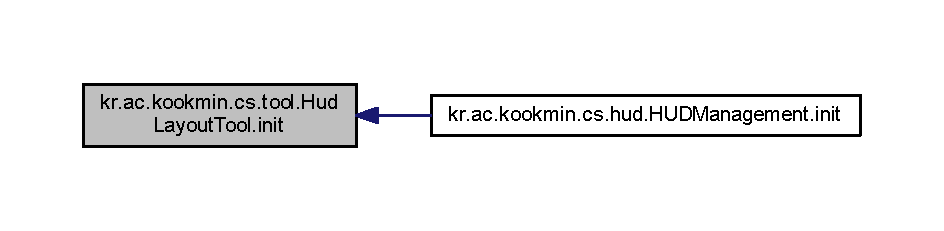
\includegraphics[width=350pt]{classkr_1_1ac_1_1kookmin_1_1cs_1_1tool_1_1_hud_layout_tool_a93ebf652629e4e65a6126d478143630b_icgraph}
\end{center}
\end{figure}


\hypertarget{classkr_1_1ac_1_1kookmin_1_1cs_1_1tool_1_1_hud_layout_tool_ac91ce5f5908a457bde5f38a847058f1d}{}\index{kr\+::ac\+::kookmin\+::cs\+::tool\+::\+Hud\+Layout\+Tool@{kr\+::ac\+::kookmin\+::cs\+::tool\+::\+Hud\+Layout\+Tool}!left\+Change@{left\+Change}}
\index{left\+Change@{left\+Change}!kr\+::ac\+::kookmin\+::cs\+::tool\+::\+Hud\+Layout\+Tool@{kr\+::ac\+::kookmin\+::cs\+::tool\+::\+Hud\+Layout\+Tool}}
\subsubsection[{left\+Change}]{\setlength{\rightskip}{0pt plus 5cm}static void kr.\+ac.\+kookmin.\+cs.\+tool.\+Hud\+Layout\+Tool.\+left\+Change (
\begin{DoxyParamCaption}
{}
\end{DoxyParamCaption}
)\hspace{0.3cm}{\ttfamily [static]}}\label{classkr_1_1ac_1_1kookmin_1_1cs_1_1tool_1_1_hud_layout_tool_ac91ce5f5908a457bde5f38a847058f1d}


This method is executed when you press the left key . 

If the mode is move, the element is moved only offset to the left . If the mode is size, the element is decreased by offset. 
\begin{DoxyParams}{매개변수}
{\em nothing} & \\
\hline
\end{DoxyParams}
\begin{DoxyReturn}{반환값}
nothing 
\end{DoxyReturn}

\begin{DoxyCode}
412   \{
413     \textcolor{keywordflow}{if}(\hyperlink{classkr_1_1ac_1_1kookmin_1_1cs_1_1tool_1_1_hud_layout_tool_a15ae154367e2b7529894488ef358f004}{elementType}==\hyperlink{classkr_1_1ac_1_1kookmin_1_1cs_1_1tool_1_1_hud_layout_tool_a58687211a1e83d17321e0ee8fc77bd6f}{PICTURE\_TYPE})
414     \{
415       PictureInfo tmp;
416       \textcolor{keywordflow}{if}(!\hyperlink{classkr_1_1ac_1_1kookmin_1_1cs_1_1tool_1_1_hud_layout_tool_acbd0f26c3534561b74d5f3b75ae4d622}{pictureList}.isEmpty()) \{
417         tmp = \hyperlink{classkr_1_1ac_1_1kookmin_1_1cs_1_1tool_1_1_hud_layout_tool_a8deeda5173478bb396d5eafd48eb5f6f}{pictureInfoList}.get(\hyperlink{classkr_1_1ac_1_1kookmin_1_1cs_1_1tool_1_1_hud_layout_tool_a1611225d44b7a53cd3a3dcf3dc85b784}{presentElementInd});
418         \textcolor{keywordflow}{if}(\hyperlink{classkr_1_1ac_1_1kookmin_1_1cs_1_1tool_1_1_hud_layout_tool_a6fb0515ee80d878c5fd737b9586772b6}{hudToolMode}==\hyperlink{classkr_1_1ac_1_1kookmin_1_1cs_1_1tool_1_1_hud_layout_tool_aecec03baf905df4aaef15cd37abe3abd}{MOVE\_MODE}) \{
419           tmp.posX-=\hyperlink{classkr_1_1ac_1_1kookmin_1_1cs_1_1tool_1_1_hud_layout_tool_a9207f2feb57881dd1d60896e45408aa5}{moveOffset};
420           \textcolor{keywordflow}{if}(tmp.posX<0)
421             tmp.posX=0;
422 
423           \hyperlink{classkr_1_1ac_1_1kookmin_1_1cs_1_1tool_1_1_hud_layout_tool_acbd0f26c3534561b74d5f3b75ae4d622}{pictureList}.get(\hyperlink{classkr_1_1ac_1_1kookmin_1_1cs_1_1tool_1_1_hud_layout_tool_a1611225d44b7a53cd3a3dcf3dc85b784}{presentElementInd}).setPosition(tmp.posX, tmp.posY);
424           \hyperlink{classkr_1_1ac_1_1kookmin_1_1cs_1_1tool_1_1_hud_layout_tool_a8deeda5173478bb396d5eafd48eb5f6f}{pictureInfoList}.get(\hyperlink{classkr_1_1ac_1_1kookmin_1_1cs_1_1tool_1_1_hud_layout_tool_a1611225d44b7a53cd3a3dcf3dc85b784}{presentElementInd}).setInfo(tmp);
425         \}
426         \textcolor{keywordflow}{else} \textcolor{keywordflow}{if}(\hyperlink{classkr_1_1ac_1_1kookmin_1_1cs_1_1tool_1_1_hud_layout_tool_a6fb0515ee80d878c5fd737b9586772b6}{hudToolMode}==\hyperlink{classkr_1_1ac_1_1kookmin_1_1cs_1_1tool_1_1_hud_layout_tool_a7072db948603a28712cb20279dc44a3a}{SIZE\_MODE}) \{
427           tmp.sizeW-=\hyperlink{classkr_1_1ac_1_1kookmin_1_1cs_1_1tool_1_1_hud_layout_tool_a9207f2feb57881dd1d60896e45408aa5}{moveOffset};
428           \textcolor{keywordflow}{if}(tmp.sizeW<0)
429             tmp.sizeW=0;
430           \hyperlink{classkr_1_1ac_1_1kookmin_1_1cs_1_1tool_1_1_hud_layout_tool_acbd0f26c3534561b74d5f3b75ae4d622}{pictureList}.get(\hyperlink{classkr_1_1ac_1_1kookmin_1_1cs_1_1tool_1_1_hud_layout_tool_a1611225d44b7a53cd3a3dcf3dc85b784}{presentElementInd}).setWidth(tmp.sizeW);
431           \hyperlink{classkr_1_1ac_1_1kookmin_1_1cs_1_1tool_1_1_hud_layout_tool_a8deeda5173478bb396d5eafd48eb5f6f}{pictureInfoList}.get(\hyperlink{classkr_1_1ac_1_1kookmin_1_1cs_1_1tool_1_1_hud_layout_tool_a1611225d44b7a53cd3a3dcf3dc85b784}{presentElementInd}).setInfo(tmp);
432         \}
433       \}
434     \}
435     \textcolor{keywordflow}{else} \textcolor{keywordflow}{if}(\hyperlink{classkr_1_1ac_1_1kookmin_1_1cs_1_1tool_1_1_hud_layout_tool_a15ae154367e2b7529894488ef358f004}{elementType}==\hyperlink{classkr_1_1ac_1_1kookmin_1_1cs_1_1tool_1_1_hud_layout_tool_abbd7ff0bb5a36036d96b889922951fd9}{TEXT\_TYPE})
436     \{
437       BitmapTextInfo tmpInfo;
438 
439       \textcolor{keywordflow}{if}(!\hyperlink{classkr_1_1ac_1_1kookmin_1_1cs_1_1tool_1_1_hud_layout_tool_a494376a3549ec46802ef2de1ebf10bc1}{textList}.isEmpty()) \{
440         tmpInfo = \hyperlink{classkr_1_1ac_1_1kookmin_1_1cs_1_1tool_1_1_hud_layout_tool_a028d96b28a4f07007430d9ac3d29eac9}{textInfoList}.get(\hyperlink{classkr_1_1ac_1_1kookmin_1_1cs_1_1tool_1_1_hud_layout_tool_ae849face952e72f68da8d09981c71c43}{presentTextInd});
441         \textcolor{keywordflow}{if}(\hyperlink{classkr_1_1ac_1_1kookmin_1_1cs_1_1tool_1_1_hud_layout_tool_a6fb0515ee80d878c5fd737b9586772b6}{hudToolMode}==\hyperlink{classkr_1_1ac_1_1kookmin_1_1cs_1_1tool_1_1_hud_layout_tool_aecec03baf905df4aaef15cd37abe3abd}{MOVE\_MODE}) \{
442           tmpInfo.posX-=\hyperlink{classkr_1_1ac_1_1kookmin_1_1cs_1_1tool_1_1_hud_layout_tool_a9207f2feb57881dd1d60896e45408aa5}{moveOffset};
443           \textcolor{keywordflow}{if}(tmpInfo.posX<0)
444             tmpInfo.posX=0;
445 
446           \hyperlink{classkr_1_1ac_1_1kookmin_1_1cs_1_1tool_1_1_hud_layout_tool_a494376a3549ec46802ef2de1ebf10bc1}{textList}.get(\hyperlink{classkr_1_1ac_1_1kookmin_1_1cs_1_1tool_1_1_hud_layout_tool_ae849face952e72f68da8d09981c71c43}{presentTextInd}).setLocalTranslation(tmpInfo.posX, tmpInfo.posY
      ,0);
447           \hyperlink{classkr_1_1ac_1_1kookmin_1_1cs_1_1tool_1_1_hud_layout_tool_a028d96b28a4f07007430d9ac3d29eac9}{textInfoList}.get(\hyperlink{classkr_1_1ac_1_1kookmin_1_1cs_1_1tool_1_1_hud_layout_tool_ae849face952e72f68da8d09981c71c43}{presentTextInd}).setInfo(tmpInfo);
448         \}
449         \textcolor{keywordflow}{else} \textcolor{keywordflow}{if}(\hyperlink{classkr_1_1ac_1_1kookmin_1_1cs_1_1tool_1_1_hud_layout_tool_a6fb0515ee80d878c5fd737b9586772b6}{hudToolMode}==\hyperlink{classkr_1_1ac_1_1kookmin_1_1cs_1_1tool_1_1_hud_layout_tool_a7072db948603a28712cb20279dc44a3a}{SIZE\_MODE}) \{
450           tmpInfo.size-=\hyperlink{classkr_1_1ac_1_1kookmin_1_1cs_1_1tool_1_1_hud_layout_tool_a9207f2feb57881dd1d60896e45408aa5}{moveOffset};
451           \textcolor{keywordflow}{if}(tmpInfo.size<0)
452             tmpInfo.size=0;
453 
454           \hyperlink{classkr_1_1ac_1_1kookmin_1_1cs_1_1tool_1_1_hud_layout_tool_a494376a3549ec46802ef2de1ebf10bc1}{textList}.get(\hyperlink{classkr_1_1ac_1_1kookmin_1_1cs_1_1tool_1_1_hud_layout_tool_ae849face952e72f68da8d09981c71c43}{presentTextInd}).setSize(tmpInfo.size);
455           \hyperlink{classkr_1_1ac_1_1kookmin_1_1cs_1_1tool_1_1_hud_layout_tool_a028d96b28a4f07007430d9ac3d29eac9}{textInfoList}.get(\hyperlink{classkr_1_1ac_1_1kookmin_1_1cs_1_1tool_1_1_hud_layout_tool_ae849face952e72f68da8d09981c71c43}{presentTextInd}).setInfo(tmpInfo);
456         \}
457       \}
458     \}
459   \}
\end{DoxyCode}
\hypertarget{classkr_1_1ac_1_1kookmin_1_1cs_1_1tool_1_1_hud_layout_tool_ae1d5a7dd1f95b43eb44b9bd1154b0eda}{}\index{kr\+::ac\+::kookmin\+::cs\+::tool\+::\+Hud\+Layout\+Tool@{kr\+::ac\+::kookmin\+::cs\+::tool\+::\+Hud\+Layout\+Tool}!pos\+And\+Size\+Print@{pos\+And\+Size\+Print}}
\index{pos\+And\+Size\+Print@{pos\+And\+Size\+Print}!kr\+::ac\+::kookmin\+::cs\+::tool\+::\+Hud\+Layout\+Tool@{kr\+::ac\+::kookmin\+::cs\+::tool\+::\+Hud\+Layout\+Tool}}
\subsubsection[{pos\+And\+Size\+Print}]{\setlength{\rightskip}{0pt plus 5cm}static void kr.\+ac.\+kookmin.\+cs.\+tool.\+Hud\+Layout\+Tool.\+pos\+And\+Size\+Print (
\begin{DoxyParamCaption}
{}
\end{DoxyParamCaption}
)\hspace{0.3cm}{\ttfamily [static]}}\label{classkr_1_1ac_1_1kookmin_1_1cs_1_1tool_1_1_hud_layout_tool_ae1d5a7dd1f95b43eb44b9bd1154b0eda}


This method outputs the size and coordinates of the selected element in the console window . 

Element Type is the case of the text, and outputs the information of the elements of Bitmap\+Text Element Type is the case of the Picture, and outputs the information of the elements of Picture. 
\begin{DoxyParams}{매개변수}
{\em nothing} & \\
\hline
\end{DoxyParams}
\begin{DoxyReturn}{반환값}
nothing 
\end{DoxyReturn}

\begin{DoxyCode}
325   \{
326     \textcolor{keywordflow}{if}(\hyperlink{classkr_1_1ac_1_1kookmin_1_1cs_1_1tool_1_1_hud_layout_tool_a15ae154367e2b7529894488ef358f004}{elementType}==\hyperlink{classkr_1_1ac_1_1kookmin_1_1cs_1_1tool_1_1_hud_layout_tool_a58687211a1e83d17321e0ee8fc77bd6f}{PICTURE\_TYPE}) \{
327       Picture tmp;
328       PictureInfo tmpInfo;
329       
330       \textcolor{keywordflow}{if}(!\hyperlink{classkr_1_1ac_1_1kookmin_1_1cs_1_1tool_1_1_hud_layout_tool_acbd0f26c3534561b74d5f3b75ae4d622}{pictureList}.isEmpty()) \{
331         tmp=\hyperlink{classkr_1_1ac_1_1kookmin_1_1cs_1_1tool_1_1_hud_layout_tool_acbd0f26c3534561b74d5f3b75ae4d622}{pictureList}.get(\hyperlink{classkr_1_1ac_1_1kookmin_1_1cs_1_1tool_1_1_hud_layout_tool_a1611225d44b7a53cd3a3dcf3dc85b784}{presentElementInd});
332         tmpInfo=\hyperlink{classkr_1_1ac_1_1kookmin_1_1cs_1_1tool_1_1_hud_layout_tool_a8deeda5173478bb396d5eafd48eb5f6f}{pictureInfoList}.get(\hyperlink{classkr_1_1ac_1_1kookmin_1_1cs_1_1tool_1_1_hud_layout_tool_a1611225d44b7a53cd3a3dcf3dc85b784}{presentElementInd});
333         System.out.print(tmp.getName()+\textcolor{stringliteral}{": pos("}+tmpInfo.posX+\textcolor{stringliteral}{", "}+tmpInfo.posY+\textcolor{stringliteral}{")"});
334         System.out.println(\textcolor{stringliteral}{" size("}+tmpInfo.sizeW+\textcolor{stringliteral}{", "}+tmpInfo.sizeH+\textcolor{stringliteral}{")"});
335       \}
336     \}
337     \textcolor{keywordflow}{else} \textcolor{keywordflow}{if}(\hyperlink{classkr_1_1ac_1_1kookmin_1_1cs_1_1tool_1_1_hud_layout_tool_a15ae154367e2b7529894488ef358f004}{elementType}==\hyperlink{classkr_1_1ac_1_1kookmin_1_1cs_1_1tool_1_1_hud_layout_tool_abbd7ff0bb5a36036d96b889922951fd9}{TEXT\_TYPE}) \{
338       BitmapText tmp;
339       BitmapTextInfo tmpInfo;
340       
341       \textcolor{keywordflow}{if}(!\hyperlink{classkr_1_1ac_1_1kookmin_1_1cs_1_1tool_1_1_hud_layout_tool_a494376a3549ec46802ef2de1ebf10bc1}{textList}.isEmpty()) \{
342         tmp=\hyperlink{classkr_1_1ac_1_1kookmin_1_1cs_1_1tool_1_1_hud_layout_tool_a494376a3549ec46802ef2de1ebf10bc1}{textList}.get(\hyperlink{classkr_1_1ac_1_1kookmin_1_1cs_1_1tool_1_1_hud_layout_tool_ae849face952e72f68da8d09981c71c43}{presentTextInd});
343         tmpInfo=\hyperlink{classkr_1_1ac_1_1kookmin_1_1cs_1_1tool_1_1_hud_layout_tool_a028d96b28a4f07007430d9ac3d29eac9}{textInfoList}.get(\hyperlink{classkr_1_1ac_1_1kookmin_1_1cs_1_1tool_1_1_hud_layout_tool_ae849face952e72f68da8d09981c71c43}{presentTextInd});
344         System.out.print(tmp.getName()+\textcolor{stringliteral}{": pos("}+tmpInfo.posX+\textcolor{stringliteral}{", "}+tmpInfo.posY+\textcolor{stringliteral}{")"});
345         System.out.println(\textcolor{stringliteral}{" size("}+tmpInfo.size+\textcolor{stringliteral}{")"});
346 
347       \}
348     \}
349   \}
\end{DoxyCode}
\hypertarget{classkr_1_1ac_1_1kookmin_1_1cs_1_1tool_1_1_hud_layout_tool_aeb639c531b592fb5d8f69fb4e033b024}{}\index{kr\+::ac\+::kookmin\+::cs\+::tool\+::\+Hud\+Layout\+Tool@{kr\+::ac\+::kookmin\+::cs\+::tool\+::\+Hud\+Layout\+Tool}!right\+Change@{right\+Change}}
\index{right\+Change@{right\+Change}!kr\+::ac\+::kookmin\+::cs\+::tool\+::\+Hud\+Layout\+Tool@{kr\+::ac\+::kookmin\+::cs\+::tool\+::\+Hud\+Layout\+Tool}}
\subsubsection[{right\+Change}]{\setlength{\rightskip}{0pt plus 5cm}static void kr.\+ac.\+kookmin.\+cs.\+tool.\+Hud\+Layout\+Tool.\+right\+Change (
\begin{DoxyParamCaption}
{}
\end{DoxyParamCaption}
)\hspace{0.3cm}{\ttfamily [static]}}\label{classkr_1_1ac_1_1kookmin_1_1cs_1_1tool_1_1_hud_layout_tool_aeb639c531b592fb5d8f69fb4e033b024}


This method is executed when you press the right key . 

If the mode is move, the element is moved only offset to the right . If the mode is size, the element is increased by offset. 
\begin{DoxyParams}{매개변수}
{\em nothing} & \\
\hline
\end{DoxyParams}
\begin{DoxyReturn}{반환값}
nothing 
\end{DoxyReturn}

\begin{DoxyCode}
360   \{
361     \textcolor{keywordflow}{if}(\hyperlink{classkr_1_1ac_1_1kookmin_1_1cs_1_1tool_1_1_hud_layout_tool_a15ae154367e2b7529894488ef358f004}{elementType}==\hyperlink{classkr_1_1ac_1_1kookmin_1_1cs_1_1tool_1_1_hud_layout_tool_a58687211a1e83d17321e0ee8fc77bd6f}{PICTURE\_TYPE}) \{
362       PictureInfo tmp;
363       \textcolor{keywordflow}{if}(!\hyperlink{classkr_1_1ac_1_1kookmin_1_1cs_1_1tool_1_1_hud_layout_tool_acbd0f26c3534561b74d5f3b75ae4d622}{pictureList}.isEmpty()) \{
364         tmp = \hyperlink{classkr_1_1ac_1_1kookmin_1_1cs_1_1tool_1_1_hud_layout_tool_a8deeda5173478bb396d5eafd48eb5f6f}{pictureInfoList}.get(\hyperlink{classkr_1_1ac_1_1kookmin_1_1cs_1_1tool_1_1_hud_layout_tool_a1611225d44b7a53cd3a3dcf3dc85b784}{presentElementInd});
365         \textcolor{keywordflow}{if}(\hyperlink{classkr_1_1ac_1_1kookmin_1_1cs_1_1tool_1_1_hud_layout_tool_a6fb0515ee80d878c5fd737b9586772b6}{hudToolMode}==\hyperlink{classkr_1_1ac_1_1kookmin_1_1cs_1_1tool_1_1_hud_layout_tool_aecec03baf905df4aaef15cd37abe3abd}{MOVE\_MODE}) \{
366           tmp.posX+=\hyperlink{classkr_1_1ac_1_1kookmin_1_1cs_1_1tool_1_1_hud_layout_tool_a9207f2feb57881dd1d60896e45408aa5}{moveOffset};
367           \textcolor{keywordflow}{if}(tmp.posX>\hyperlink{classkr_1_1ac_1_1kookmin_1_1cs_1_1tool_1_1_hud_layout_tool_af06a05d18241dcbe2bc4f2c96d157ee0}{sim}.getSettings().getWidth())
368             tmp.posX=\hyperlink{classkr_1_1ac_1_1kookmin_1_1cs_1_1tool_1_1_hud_layout_tool_af06a05d18241dcbe2bc4f2c96d157ee0}{sim}.getSettings().getWidth();
369 
370           \hyperlink{classkr_1_1ac_1_1kookmin_1_1cs_1_1tool_1_1_hud_layout_tool_acbd0f26c3534561b74d5f3b75ae4d622}{pictureList}.get(\hyperlink{classkr_1_1ac_1_1kookmin_1_1cs_1_1tool_1_1_hud_layout_tool_a1611225d44b7a53cd3a3dcf3dc85b784}{presentElementInd}).setPosition(tmp.posX, tmp.posY);
371           \hyperlink{classkr_1_1ac_1_1kookmin_1_1cs_1_1tool_1_1_hud_layout_tool_a8deeda5173478bb396d5eafd48eb5f6f}{pictureInfoList}.get(\hyperlink{classkr_1_1ac_1_1kookmin_1_1cs_1_1tool_1_1_hud_layout_tool_a1611225d44b7a53cd3a3dcf3dc85b784}{presentElementInd}).setInfo(tmp);
372         \}
373         \textcolor{keywordflow}{else} \textcolor{keywordflow}{if}(\hyperlink{classkr_1_1ac_1_1kookmin_1_1cs_1_1tool_1_1_hud_layout_tool_a6fb0515ee80d878c5fd737b9586772b6}{hudToolMode}==\hyperlink{classkr_1_1ac_1_1kookmin_1_1cs_1_1tool_1_1_hud_layout_tool_a7072db948603a28712cb20279dc44a3a}{SIZE\_MODE}) \{
374           tmp.sizeW+=\hyperlink{classkr_1_1ac_1_1kookmin_1_1cs_1_1tool_1_1_hud_layout_tool_a9207f2feb57881dd1d60896e45408aa5}{moveOffset};
375 
376           \hyperlink{classkr_1_1ac_1_1kookmin_1_1cs_1_1tool_1_1_hud_layout_tool_acbd0f26c3534561b74d5f3b75ae4d622}{pictureList}.get(\hyperlink{classkr_1_1ac_1_1kookmin_1_1cs_1_1tool_1_1_hud_layout_tool_a1611225d44b7a53cd3a3dcf3dc85b784}{presentElementInd}).setWidth(tmp.sizeW);
377           \hyperlink{classkr_1_1ac_1_1kookmin_1_1cs_1_1tool_1_1_hud_layout_tool_a8deeda5173478bb396d5eafd48eb5f6f}{pictureInfoList}.get(\hyperlink{classkr_1_1ac_1_1kookmin_1_1cs_1_1tool_1_1_hud_layout_tool_a1611225d44b7a53cd3a3dcf3dc85b784}{presentElementInd}).setInfo(tmp);
378         \}
379       \}
380     \}
381     \textcolor{keywordflow}{else} \textcolor{keywordflow}{if}(\hyperlink{classkr_1_1ac_1_1kookmin_1_1cs_1_1tool_1_1_hud_layout_tool_a15ae154367e2b7529894488ef358f004}{elementType}==\hyperlink{classkr_1_1ac_1_1kookmin_1_1cs_1_1tool_1_1_hud_layout_tool_abbd7ff0bb5a36036d96b889922951fd9}{TEXT\_TYPE}) \{
382       BitmapTextInfo tmpInfo;
383 
384       \textcolor{keywordflow}{if}(!\hyperlink{classkr_1_1ac_1_1kookmin_1_1cs_1_1tool_1_1_hud_layout_tool_a494376a3549ec46802ef2de1ebf10bc1}{textList}.isEmpty()) \{
385         tmpInfo = \hyperlink{classkr_1_1ac_1_1kookmin_1_1cs_1_1tool_1_1_hud_layout_tool_a028d96b28a4f07007430d9ac3d29eac9}{textInfoList}.get(\hyperlink{classkr_1_1ac_1_1kookmin_1_1cs_1_1tool_1_1_hud_layout_tool_ae849face952e72f68da8d09981c71c43}{presentTextInd});
386         \textcolor{keywordflow}{if}(\hyperlink{classkr_1_1ac_1_1kookmin_1_1cs_1_1tool_1_1_hud_layout_tool_a6fb0515ee80d878c5fd737b9586772b6}{hudToolMode}==\hyperlink{classkr_1_1ac_1_1kookmin_1_1cs_1_1tool_1_1_hud_layout_tool_aecec03baf905df4aaef15cd37abe3abd}{MOVE\_MODE}) \{
387           tmpInfo.posX+=\hyperlink{classkr_1_1ac_1_1kookmin_1_1cs_1_1tool_1_1_hud_layout_tool_a9207f2feb57881dd1d60896e45408aa5}{moveOffset};
388           \textcolor{keywordflow}{if}(tmpInfo.posX>\hyperlink{classkr_1_1ac_1_1kookmin_1_1cs_1_1tool_1_1_hud_layout_tool_af06a05d18241dcbe2bc4f2c96d157ee0}{sim}.getSettings().getWidth())
389             tmpInfo.posX=\hyperlink{classkr_1_1ac_1_1kookmin_1_1cs_1_1tool_1_1_hud_layout_tool_af06a05d18241dcbe2bc4f2c96d157ee0}{sim}.getSettings().getWidth();
390 
391           \hyperlink{classkr_1_1ac_1_1kookmin_1_1cs_1_1tool_1_1_hud_layout_tool_a494376a3549ec46802ef2de1ebf10bc1}{textList}.get(\hyperlink{classkr_1_1ac_1_1kookmin_1_1cs_1_1tool_1_1_hud_layout_tool_ae849face952e72f68da8d09981c71c43}{presentTextInd}).setLocalTranslation(tmpInfo.posX, tmpInfo.posY
      ,0);
392           \hyperlink{classkr_1_1ac_1_1kookmin_1_1cs_1_1tool_1_1_hud_layout_tool_a028d96b28a4f07007430d9ac3d29eac9}{textInfoList}.get(\hyperlink{classkr_1_1ac_1_1kookmin_1_1cs_1_1tool_1_1_hud_layout_tool_ae849face952e72f68da8d09981c71c43}{presentTextInd}).setInfo(tmpInfo);
393         \}
394         \textcolor{keywordflow}{else} \textcolor{keywordflow}{if}(\hyperlink{classkr_1_1ac_1_1kookmin_1_1cs_1_1tool_1_1_hud_layout_tool_a6fb0515ee80d878c5fd737b9586772b6}{hudToolMode}==\hyperlink{classkr_1_1ac_1_1kookmin_1_1cs_1_1tool_1_1_hud_layout_tool_a7072db948603a28712cb20279dc44a3a}{SIZE\_MODE}) \{
395           tmpInfo.size+=\hyperlink{classkr_1_1ac_1_1kookmin_1_1cs_1_1tool_1_1_hud_layout_tool_a9207f2feb57881dd1d60896e45408aa5}{moveOffset};
396 
397           \hyperlink{classkr_1_1ac_1_1kookmin_1_1cs_1_1tool_1_1_hud_layout_tool_a494376a3549ec46802ef2de1ebf10bc1}{textList}.get(\hyperlink{classkr_1_1ac_1_1kookmin_1_1cs_1_1tool_1_1_hud_layout_tool_ae849face952e72f68da8d09981c71c43}{presentTextInd}).setSize(tmpInfo.size);
398           \hyperlink{classkr_1_1ac_1_1kookmin_1_1cs_1_1tool_1_1_hud_layout_tool_a028d96b28a4f07007430d9ac3d29eac9}{textInfoList}.get(\hyperlink{classkr_1_1ac_1_1kookmin_1_1cs_1_1tool_1_1_hud_layout_tool_ae849face952e72f68da8d09981c71c43}{presentTextInd}).setInfo(tmpInfo);
399         \}
400       \}
401     \}
402 
403   \}
\end{DoxyCode}
\hypertarget{classkr_1_1ac_1_1kookmin_1_1cs_1_1tool_1_1_hud_layout_tool_a8088ea305a4ba9df53b6bad090655e36}{}\index{kr\+::ac\+::kookmin\+::cs\+::tool\+::\+Hud\+Layout\+Tool@{kr\+::ac\+::kookmin\+::cs\+::tool\+::\+Hud\+Layout\+Tool}!select\+Element\+Type@{select\+Element\+Type}}
\index{select\+Element\+Type@{select\+Element\+Type}!kr\+::ac\+::kookmin\+::cs\+::tool\+::\+Hud\+Layout\+Tool@{kr\+::ac\+::kookmin\+::cs\+::tool\+::\+Hud\+Layout\+Tool}}
\subsubsection[{select\+Element\+Type}]{\setlength{\rightskip}{0pt plus 5cm}static void kr.\+ac.\+kookmin.\+cs.\+tool.\+Hud\+Layout\+Tool.\+select\+Element\+Type (
\begin{DoxyParamCaption}
{}
\end{DoxyParamCaption}
)\hspace{0.3cm}{\ttfamily [static]}}\label{classkr_1_1ac_1_1kookmin_1_1cs_1_1tool_1_1_hud_layout_tool_a8088ea305a4ba9df53b6bad090655e36}


This method , to select the element type . 

If the element type is picture type, it converted to the text type else if the element type is text type, it converted to the picture type 
\begin{DoxyParams}{매개변수}
{\em nothing} & \\
\hline
\end{DoxyParams}
\begin{DoxyReturn}{반환값}
nothing 
\end{DoxyReturn}

\begin{DoxyCode}
595   \{
596     \textcolor{keywordflow}{if}(\hyperlink{classkr_1_1ac_1_1kookmin_1_1cs_1_1tool_1_1_hud_layout_tool_a15ae154367e2b7529894488ef358f004}{elementType}==\hyperlink{classkr_1_1ac_1_1kookmin_1_1cs_1_1tool_1_1_hud_layout_tool_a58687211a1e83d17321e0ee8fc77bd6f}{PICTURE\_TYPE})
597       \hyperlink{classkr_1_1ac_1_1kookmin_1_1cs_1_1tool_1_1_hud_layout_tool_a15ae154367e2b7529894488ef358f004}{elementType}=\hyperlink{classkr_1_1ac_1_1kookmin_1_1cs_1_1tool_1_1_hud_layout_tool_abbd7ff0bb5a36036d96b889922951fd9}{TEXT\_TYPE};
598     \textcolor{keywordflow}{else}
599       \hyperlink{classkr_1_1ac_1_1kookmin_1_1cs_1_1tool_1_1_hud_layout_tool_a15ae154367e2b7529894488ef358f004}{elementType}=\hyperlink{classkr_1_1ac_1_1kookmin_1_1cs_1_1tool_1_1_hud_layout_tool_a58687211a1e83d17321e0ee8fc77bd6f}{PICTURE\_TYPE};
600   \}
\end{DoxyCode}
\hypertarget{classkr_1_1ac_1_1kookmin_1_1cs_1_1tool_1_1_hud_layout_tool_aed1bf1517f60598e90f982d837fbb4b1}{}\index{kr\+::ac\+::kookmin\+::cs\+::tool\+::\+Hud\+Layout\+Tool@{kr\+::ac\+::kookmin\+::cs\+::tool\+::\+Hud\+Layout\+Tool}!select\+Mode@{select\+Mode}}
\index{select\+Mode@{select\+Mode}!kr\+::ac\+::kookmin\+::cs\+::tool\+::\+Hud\+Layout\+Tool@{kr\+::ac\+::kookmin\+::cs\+::tool\+::\+Hud\+Layout\+Tool}}
\subsubsection[{select\+Mode}]{\setlength{\rightskip}{0pt plus 5cm}static void kr.\+ac.\+kookmin.\+cs.\+tool.\+Hud\+Layout\+Tool.\+select\+Mode (
\begin{DoxyParamCaption}
{}
\end{DoxyParamCaption}
)\hspace{0.3cm}{\ttfamily [static]}}\label{classkr_1_1ac_1_1kookmin_1_1cs_1_1tool_1_1_hud_layout_tool_aed1bf1517f60598e90f982d837fbb4b1}


This method , to select the mode . 

If the mode is move, it converted to the size mode else if the mode is size, it converted to the move mode 
\begin{DoxyParams}{매개변수}
{\em nothing} & \\
\hline
\end{DoxyParams}
\begin{DoxyReturn}{반환값}
nothing 
\end{DoxyReturn}

\begin{DoxyCode}
579   \{
580     \textcolor{keywordflow}{if}(\hyperlink{classkr_1_1ac_1_1kookmin_1_1cs_1_1tool_1_1_hud_layout_tool_a6fb0515ee80d878c5fd737b9586772b6}{hudToolMode}==\hyperlink{classkr_1_1ac_1_1kookmin_1_1cs_1_1tool_1_1_hud_layout_tool_aecec03baf905df4aaef15cd37abe3abd}{MOVE\_MODE})
581       \hyperlink{classkr_1_1ac_1_1kookmin_1_1cs_1_1tool_1_1_hud_layout_tool_a6fb0515ee80d878c5fd737b9586772b6}{hudToolMode}=\hyperlink{classkr_1_1ac_1_1kookmin_1_1cs_1_1tool_1_1_hud_layout_tool_a7072db948603a28712cb20279dc44a3a}{SIZE\_MODE};
582     \textcolor{keywordflow}{else}
583       \hyperlink{classkr_1_1ac_1_1kookmin_1_1cs_1_1tool_1_1_hud_layout_tool_a6fb0515ee80d878c5fd737b9586772b6}{hudToolMode}=\hyperlink{classkr_1_1ac_1_1kookmin_1_1cs_1_1tool_1_1_hud_layout_tool_aecec03baf905df4aaef15cd37abe3abd}{MOVE\_MODE};
584   \}
\end{DoxyCode}
\hypertarget{classkr_1_1ac_1_1kookmin_1_1cs_1_1tool_1_1_hud_layout_tool_a6f5f4dcaf3b5aeee139ab80fb3aa30aa}{}\index{kr\+::ac\+::kookmin\+::cs\+::tool\+::\+Hud\+Layout\+Tool@{kr\+::ac\+::kookmin\+::cs\+::tool\+::\+Hud\+Layout\+Tool}!start\+Hud\+Tool@{start\+Hud\+Tool}}
\index{start\+Hud\+Tool@{start\+Hud\+Tool}!kr\+::ac\+::kookmin\+::cs\+::tool\+::\+Hud\+Layout\+Tool@{kr\+::ac\+::kookmin\+::cs\+::tool\+::\+Hud\+Layout\+Tool}}
\subsubsection[{start\+Hud\+Tool}]{\setlength{\rightskip}{0pt plus 5cm}static void kr.\+ac.\+kookmin.\+cs.\+tool.\+Hud\+Layout\+Tool.\+start\+Hud\+Tool (
\begin{DoxyParamCaption}
{}
\end{DoxyParamCaption}
)\hspace{0.3cm}{\ttfamily [static]}}\label{classkr_1_1ac_1_1kookmin_1_1cs_1_1tool_1_1_hud_layout_tool_a6f5f4dcaf3b5aeee139ab80fb3aa30aa}


This method is executed the \hyperlink{classkr_1_1ac_1_1kookmin_1_1cs_1_1tool_1_1_hud_layout_tool}{Hud\+Layout\+Tool} mode at startup . 

Read the path of use .png file and .text file as the element from /assets/\+Tool directory .png file is assigned to Picture element, .txt file is assigned to Bitmap\+Text element and , this element managed to Array\+List. 
\begin{DoxyParams}{매개변수}
{\em nothing} & \\
\hline
\end{DoxyParams}
\begin{DoxyReturn}{반환값}
nothing 
\end{DoxyReturn}

\begin{DoxyCode}
97   \{
98     \textcolor{comment}{// path:current\_workingdir\(\backslash\)assets\(\backslash\)Tool}
99     \textcolor{comment}{// find to file list in path }
100     String path=System.getProperty(\textcolor{stringliteral}{"user.dir"});
101     path+=\textcolor{stringliteral}{"\(\backslash\)\(\backslash\)assets\(\backslash\)\(\backslash\)Tool"};
102     File dir = \textcolor{keyword}{new} File(path);
103     File[] filelist = dir.listFiles();
104     
105     \textcolor{keywordflow}{for}(File file:filelist)
106     \{
107       \textcolor{keywordflow}{if}(file.isFile() && file.getName().endsWith(\textcolor{stringliteral}{".png"})) \{
108         \hyperlink{classkr_1_1ac_1_1kookmin_1_1cs_1_1tool_1_1_hud_layout_tool_acbd0f26c3534561b74d5f3b75ae4d622}{pictureList}.add(\textcolor{keyword}{new} Picture(file.getName()));
109         BufferedImage bimg;
110         \textcolor{keywordflow}{try} \{
111           bimg = ImageIO.read(\textcolor{keyword}{new} File(file.getPath()));
112           \hyperlink{classkr_1_1ac_1_1kookmin_1_1cs_1_1tool_1_1_hud_layout_tool_a8deeda5173478bb396d5eafd48eb5f6f}{pictureInfoList}.add(\textcolor{keyword}{new} PictureInfo(\hyperlink{classkr_1_1ac_1_1kookmin_1_1cs_1_1tool_1_1_hud_layout_tool_af06a05d18241dcbe2bc4f2c96d157ee0}{sim}.getSettings().getWidth()/2, 
      \hyperlink{classkr_1_1ac_1_1kookmin_1_1cs_1_1tool_1_1_hud_layout_tool_af06a05d18241dcbe2bc4f2c96d157ee0}{sim}.getSettings().getHeight()/2,bimg.getWidth(),bimg.getHeight()));
113         \} \textcolor{keywordflow}{catch} (IOException e) \{
114           e.printStackTrace();
115         \}
116       \}
117       \textcolor{keywordflow}{else} \textcolor{keywordflow}{if}(file.isFile() && file.getName().endsWith(\textcolor{stringliteral}{".txt"})) \{
118         BufferedReader in;
119         String str=\textcolor{stringliteral}{""},s;
120         
121         \textcolor{keywordflow}{try} \{
122           \textcolor{comment}{// file Read}
123           in = \textcolor{keyword}{new} BufferedReader(\textcolor{keyword}{new} FileReader(file));
124           \textcolor{keywordflow}{while}((s=in.readLine()) !=null)
125             str+=s+\textcolor{stringliteral}{"\(\backslash\)n"};
126         \} \textcolor{keywordflow}{catch} (FileNotFoundException e) \{
127           e.printStackTrace();
128         \} \textcolor{keywordflow}{catch} (IOException e) \{
129           e.printStackTrace();
130         \}
131         \textcolor{comment}{// initial part}
132         BitmapText tmpText=\textcolor{keyword}{new} BitmapText(\hyperlink{classkr_1_1ac_1_1kookmin_1_1cs_1_1tool_1_1_hud_layout_tool_a92b0ab831e8b62aaebc0974947958349}{guiFont},\textcolor{keyword}{false});
133         tmpText.setName(file.getName());
134         tmpText.setText(str);
135         System.out.println(str);
136         tmpText.setColor(ColorRGBA.White);
137         tmpText.setSize(\hyperlink{classkr_1_1ac_1_1kookmin_1_1cs_1_1tool_1_1_hud_layout_tool_a92b0ab831e8b62aaebc0974947958349}{guiFont}.getCharSet().getRenderedSize());
138         tmpText.setLocalTranslation(\hyperlink{classkr_1_1ac_1_1kookmin_1_1cs_1_1tool_1_1_hud_layout_tool_af06a05d18241dcbe2bc4f2c96d157ee0}{sim}.getSettings().getWidth()/2, \hyperlink{classkr_1_1ac_1_1kookmin_1_1cs_1_1tool_1_1_hud_layout_tool_af06a05d18241dcbe2bc4f2c96d157ee0}{sim}.getSettings().getHeight()/2, 
      0);
139 
140         \textcolor{comment}{// add element in textlist}
141         \hyperlink{classkr_1_1ac_1_1kookmin_1_1cs_1_1tool_1_1_hud_layout_tool_a494376a3549ec46802ef2de1ebf10bc1}{textList}.add(tmpText);
142         \hyperlink{classkr_1_1ac_1_1kookmin_1_1cs_1_1tool_1_1_hud_layout_tool_a028d96b28a4f07007430d9ac3d29eac9}{textInfoList}.add(\textcolor{keyword}{new} BitmapTextInfo(\hyperlink{classkr_1_1ac_1_1kookmin_1_1cs_1_1tool_1_1_hud_layout_tool_af06a05d18241dcbe2bc4f2c96d157ee0}{sim}.getSettings().getWidth()/2,
      \hyperlink{classkr_1_1ac_1_1kookmin_1_1cs_1_1tool_1_1_hud_layout_tool_af06a05d18241dcbe2bc4f2c96d157ee0}{sim}.getSettings().getHeight()/2,\hyperlink{classkr_1_1ac_1_1kookmin_1_1cs_1_1tool_1_1_hud_layout_tool_a92b0ab831e8b62aaebc0974947958349}{guiFont}.getCharSet().getRenderedSize()));
143 
144       \}
145 
146     \}
147 
148     path=\textcolor{stringliteral}{"Tool/"};
149     \textcolor{keywordtype}{int} i=0;
150     \textcolor{comment}{// each element initialization}
151     \textcolor{keywordflow}{for}(Picture tmp:\hyperlink{classkr_1_1ac_1_1kookmin_1_1cs_1_1tool_1_1_hud_layout_tool_acbd0f26c3534561b74d5f3b75ae4d622}{pictureList}) \{
152       PictureInfo info=\hyperlink{classkr_1_1ac_1_1kookmin_1_1cs_1_1tool_1_1_hud_layout_tool_a8deeda5173478bb396d5eafd48eb5f6f}{pictureInfoList}.get(i++);
153       tmp.setImage(\hyperlink{classkr_1_1ac_1_1kookmin_1_1cs_1_1tool_1_1_hud_layout_tool_af06a05d18241dcbe2bc4f2c96d157ee0}{sim}.getAssetManager(), path+tmp.getName(), \textcolor{keyword}{true});
154       tmp.setHeight(info.sizeH);
155       tmp.setWidth(info.sizeW);
156       tmp.setPosition(info.posX,info.posY);
157     \}
158 
159     \hyperlink{classkr_1_1ac_1_1kookmin_1_1cs_1_1tool_1_1_hud_layout_tool_a48bdb0935f0a1b47acdd97d4ea4adab6}{hudToolActF}=\textcolor{keyword}{true};
160   \}
\end{DoxyCode}
\hypertarget{classkr_1_1ac_1_1kookmin_1_1cs_1_1tool_1_1_hud_layout_tool_aea6f75ea2479a569dfa99c849df7b435}{}\index{kr\+::ac\+::kookmin\+::cs\+::tool\+::\+Hud\+Layout\+Tool@{kr\+::ac\+::kookmin\+::cs\+::tool\+::\+Hud\+Layout\+Tool}!up\+Change@{up\+Change}}
\index{up\+Change@{up\+Change}!kr\+::ac\+::kookmin\+::cs\+::tool\+::\+Hud\+Layout\+Tool@{kr\+::ac\+::kookmin\+::cs\+::tool\+::\+Hud\+Layout\+Tool}}
\subsubsection[{up\+Change}]{\setlength{\rightskip}{0pt plus 5cm}static void kr.\+ac.\+kookmin.\+cs.\+tool.\+Hud\+Layout\+Tool.\+up\+Change (
\begin{DoxyParamCaption}
{}
\end{DoxyParamCaption}
)\hspace{0.3cm}{\ttfamily [static]}}\label{classkr_1_1ac_1_1kookmin_1_1cs_1_1tool_1_1_hud_layout_tool_aea6f75ea2479a569dfa99c849df7b435}


This method is executed when you press the up key . 

If the mode is move, the element is moved only offset to the up . If the mode is size, the element is increased by offset. 
\begin{DoxyParams}{매개변수}
{\em nothing} & \\
\hline
\end{DoxyParams}
\begin{DoxyReturn}{반환값}
nothing 
\end{DoxyReturn}

\begin{DoxyCode}
468   \{
469     \textcolor{keywordflow}{if}(\hyperlink{classkr_1_1ac_1_1kookmin_1_1cs_1_1tool_1_1_hud_layout_tool_a15ae154367e2b7529894488ef358f004}{elementType}==\hyperlink{classkr_1_1ac_1_1kookmin_1_1cs_1_1tool_1_1_hud_layout_tool_a58687211a1e83d17321e0ee8fc77bd6f}{PICTURE\_TYPE}) \{
470       PictureInfo tmp;
471       \textcolor{keywordflow}{if}(!\hyperlink{classkr_1_1ac_1_1kookmin_1_1cs_1_1tool_1_1_hud_layout_tool_acbd0f26c3534561b74d5f3b75ae4d622}{pictureList}.isEmpty()) \{
472         tmp = \hyperlink{classkr_1_1ac_1_1kookmin_1_1cs_1_1tool_1_1_hud_layout_tool_a8deeda5173478bb396d5eafd48eb5f6f}{pictureInfoList}.get(\hyperlink{classkr_1_1ac_1_1kookmin_1_1cs_1_1tool_1_1_hud_layout_tool_a1611225d44b7a53cd3a3dcf3dc85b784}{presentElementInd});
473         \textcolor{keywordflow}{if}(\hyperlink{classkr_1_1ac_1_1kookmin_1_1cs_1_1tool_1_1_hud_layout_tool_a6fb0515ee80d878c5fd737b9586772b6}{hudToolMode}==\hyperlink{classkr_1_1ac_1_1kookmin_1_1cs_1_1tool_1_1_hud_layout_tool_aecec03baf905df4aaef15cd37abe3abd}{MOVE\_MODE}) \{
474           tmp.posY+=\hyperlink{classkr_1_1ac_1_1kookmin_1_1cs_1_1tool_1_1_hud_layout_tool_a9207f2feb57881dd1d60896e45408aa5}{moveOffset};
475           \textcolor{keywordflow}{if}(tmp.posY>\hyperlink{classkr_1_1ac_1_1kookmin_1_1cs_1_1tool_1_1_hud_layout_tool_af06a05d18241dcbe2bc4f2c96d157ee0}{sim}.getSettings().getHeight())
476             tmp.posY=\hyperlink{classkr_1_1ac_1_1kookmin_1_1cs_1_1tool_1_1_hud_layout_tool_af06a05d18241dcbe2bc4f2c96d157ee0}{sim}.getSettings().getHeight();
477 
478           \hyperlink{classkr_1_1ac_1_1kookmin_1_1cs_1_1tool_1_1_hud_layout_tool_acbd0f26c3534561b74d5f3b75ae4d622}{pictureList}.get(\hyperlink{classkr_1_1ac_1_1kookmin_1_1cs_1_1tool_1_1_hud_layout_tool_a1611225d44b7a53cd3a3dcf3dc85b784}{presentElementInd}).setPosition(tmp.posX, tmp.posY);
479           \hyperlink{classkr_1_1ac_1_1kookmin_1_1cs_1_1tool_1_1_hud_layout_tool_a8deeda5173478bb396d5eafd48eb5f6f}{pictureInfoList}.get(\hyperlink{classkr_1_1ac_1_1kookmin_1_1cs_1_1tool_1_1_hud_layout_tool_a1611225d44b7a53cd3a3dcf3dc85b784}{presentElementInd}).setInfo(tmp);
480         \}
481         \textcolor{keywordflow}{else} \textcolor{keywordflow}{if}(\hyperlink{classkr_1_1ac_1_1kookmin_1_1cs_1_1tool_1_1_hud_layout_tool_a6fb0515ee80d878c5fd737b9586772b6}{hudToolMode}==\hyperlink{classkr_1_1ac_1_1kookmin_1_1cs_1_1tool_1_1_hud_layout_tool_a7072db948603a28712cb20279dc44a3a}{SIZE\_MODE}) \{
482           tmp.sizeH+=\hyperlink{classkr_1_1ac_1_1kookmin_1_1cs_1_1tool_1_1_hud_layout_tool_a9207f2feb57881dd1d60896e45408aa5}{moveOffset};
483 
484           \hyperlink{classkr_1_1ac_1_1kookmin_1_1cs_1_1tool_1_1_hud_layout_tool_acbd0f26c3534561b74d5f3b75ae4d622}{pictureList}.get(\hyperlink{classkr_1_1ac_1_1kookmin_1_1cs_1_1tool_1_1_hud_layout_tool_a1611225d44b7a53cd3a3dcf3dc85b784}{presentElementInd}).setHeight(tmp.sizeH);
485           \hyperlink{classkr_1_1ac_1_1kookmin_1_1cs_1_1tool_1_1_hud_layout_tool_a8deeda5173478bb396d5eafd48eb5f6f}{pictureInfoList}.get(\hyperlink{classkr_1_1ac_1_1kookmin_1_1cs_1_1tool_1_1_hud_layout_tool_a1611225d44b7a53cd3a3dcf3dc85b784}{presentElementInd}).setInfo(tmp);
486         \}
487       \}
488     \}
489     \textcolor{keywordflow}{else} \textcolor{keywordflow}{if}(\hyperlink{classkr_1_1ac_1_1kookmin_1_1cs_1_1tool_1_1_hud_layout_tool_a15ae154367e2b7529894488ef358f004}{elementType}==\hyperlink{classkr_1_1ac_1_1kookmin_1_1cs_1_1tool_1_1_hud_layout_tool_abbd7ff0bb5a36036d96b889922951fd9}{TEXT\_TYPE}) \{
490       BitmapTextInfo tmpInfo;
491 
492       \textcolor{keywordflow}{if}(!\hyperlink{classkr_1_1ac_1_1kookmin_1_1cs_1_1tool_1_1_hud_layout_tool_a494376a3549ec46802ef2de1ebf10bc1}{textList}.isEmpty()) \{
493         tmpInfo = \hyperlink{classkr_1_1ac_1_1kookmin_1_1cs_1_1tool_1_1_hud_layout_tool_a028d96b28a4f07007430d9ac3d29eac9}{textInfoList}.get(\hyperlink{classkr_1_1ac_1_1kookmin_1_1cs_1_1tool_1_1_hud_layout_tool_ae849face952e72f68da8d09981c71c43}{presentTextInd});
494         \textcolor{keywordflow}{if}(\hyperlink{classkr_1_1ac_1_1kookmin_1_1cs_1_1tool_1_1_hud_layout_tool_a6fb0515ee80d878c5fd737b9586772b6}{hudToolMode}==\hyperlink{classkr_1_1ac_1_1kookmin_1_1cs_1_1tool_1_1_hud_layout_tool_aecec03baf905df4aaef15cd37abe3abd}{MOVE\_MODE}) \{
495           tmpInfo.posY+=\hyperlink{classkr_1_1ac_1_1kookmin_1_1cs_1_1tool_1_1_hud_layout_tool_a9207f2feb57881dd1d60896e45408aa5}{moveOffset};
496           \textcolor{keywordflow}{if}(tmpInfo.posY>\hyperlink{classkr_1_1ac_1_1kookmin_1_1cs_1_1tool_1_1_hud_layout_tool_af06a05d18241dcbe2bc4f2c96d157ee0}{sim}.getSettings().getHeight())
497             tmpInfo.posY=\hyperlink{classkr_1_1ac_1_1kookmin_1_1cs_1_1tool_1_1_hud_layout_tool_af06a05d18241dcbe2bc4f2c96d157ee0}{sim}.getSettings().getHeight();
498 
499           \hyperlink{classkr_1_1ac_1_1kookmin_1_1cs_1_1tool_1_1_hud_layout_tool_a494376a3549ec46802ef2de1ebf10bc1}{textList}.get(\hyperlink{classkr_1_1ac_1_1kookmin_1_1cs_1_1tool_1_1_hud_layout_tool_ae849face952e72f68da8d09981c71c43}{presentTextInd}).setLocalTranslation(tmpInfo.posX, tmpInfo.posY
      ,0);
500           \hyperlink{classkr_1_1ac_1_1kookmin_1_1cs_1_1tool_1_1_hud_layout_tool_a028d96b28a4f07007430d9ac3d29eac9}{textInfoList}.get(\hyperlink{classkr_1_1ac_1_1kookmin_1_1cs_1_1tool_1_1_hud_layout_tool_ae849face952e72f68da8d09981c71c43}{presentTextInd}).setInfo(tmpInfo);
501         \}
502         \textcolor{keywordflow}{else} \textcolor{keywordflow}{if}(\hyperlink{classkr_1_1ac_1_1kookmin_1_1cs_1_1tool_1_1_hud_layout_tool_a6fb0515ee80d878c5fd737b9586772b6}{hudToolMode}==\hyperlink{classkr_1_1ac_1_1kookmin_1_1cs_1_1tool_1_1_hud_layout_tool_a7072db948603a28712cb20279dc44a3a}{SIZE\_MODE}) \{
503           tmpInfo.size+=\hyperlink{classkr_1_1ac_1_1kookmin_1_1cs_1_1tool_1_1_hud_layout_tool_a9207f2feb57881dd1d60896e45408aa5}{moveOffset};
504 
505           \hyperlink{classkr_1_1ac_1_1kookmin_1_1cs_1_1tool_1_1_hud_layout_tool_a494376a3549ec46802ef2de1ebf10bc1}{textList}.get(\hyperlink{classkr_1_1ac_1_1kookmin_1_1cs_1_1tool_1_1_hud_layout_tool_ae849face952e72f68da8d09981c71c43}{presentTextInd}).setSize(tmpInfo.size);
506           \hyperlink{classkr_1_1ac_1_1kookmin_1_1cs_1_1tool_1_1_hud_layout_tool_a028d96b28a4f07007430d9ac3d29eac9}{textInfoList}.get(\hyperlink{classkr_1_1ac_1_1kookmin_1_1cs_1_1tool_1_1_hud_layout_tool_ae849face952e72f68da8d09981c71c43}{presentTextInd}).setInfo(tmpInfo);
507         \}
508       \}
509 
510     \}
511 
512   \}
\end{DoxyCode}
\hypertarget{classkr_1_1ac_1_1kookmin_1_1cs_1_1tool_1_1_hud_layout_tool_a1206c4b2c371bbbe24cf257492826574}{}\index{kr\+::ac\+::kookmin\+::cs\+::tool\+::\+Hud\+Layout\+Tool@{kr\+::ac\+::kookmin\+::cs\+::tool\+::\+Hud\+Layout\+Tool}!updating\+Hud\+Tool@{updating\+Hud\+Tool}}
\index{updating\+Hud\+Tool@{updating\+Hud\+Tool}!kr\+::ac\+::kookmin\+::cs\+::tool\+::\+Hud\+Layout\+Tool@{kr\+::ac\+::kookmin\+::cs\+::tool\+::\+Hud\+Layout\+Tool}}
\subsubsection[{updating\+Hud\+Tool}]{\setlength{\rightskip}{0pt plus 5cm}static void kr.\+ac.\+kookmin.\+cs.\+tool.\+Hud\+Layout\+Tool.\+updating\+Hud\+Tool (
\begin{DoxyParamCaption}
{}
\end{DoxyParamCaption}
)\hspace{0.3cm}{\ttfamily [static]}}\label{classkr_1_1ac_1_1kookmin_1_1cs_1_1tool_1_1_hud_layout_tool_a1206c4b2c371bbbe24cf257492826574}


Is a method to be executed in real time on the simulator . 

It will update the mode and offset size and element type of Hud\+Tool. 
\begin{DoxyParams}{매개변수}
{\em nothing} & \\
\hline
\end{DoxyParams}
\begin{DoxyReturn}{반환값}
nothing 
\end{DoxyReturn}

\begin{DoxyCode}
170   \{
171     \textcolor{keywordflow}{if}(HudLayoutTool.hudToolActF) \{
172       \textcolor{comment}{//print move offset}
173       String tmp =\textcolor{stringliteral}{"moveOffset: "}+String.valueOf(\hyperlink{classkr_1_1ac_1_1kookmin_1_1cs_1_1tool_1_1_hud_layout_tool_a9207f2feb57881dd1d60896e45408aa5}{moveOffset})+\textcolor{stringliteral}{"\(\backslash\)n"}+\textcolor{stringliteral}{"element Type:"};
174       \textcolor{keywordflow}{if}(\hyperlink{classkr_1_1ac_1_1kookmin_1_1cs_1_1tool_1_1_hud_layout_tool_a15ae154367e2b7529894488ef358f004}{elementType}==\hyperlink{classkr_1_1ac_1_1kookmin_1_1cs_1_1tool_1_1_hud_layout_tool_a58687211a1e83d17321e0ee8fc77bd6f}{PICTURE\_TYPE})
175         tmp+=\textcolor{stringliteral}{"PICTURE"}+\textcolor{stringliteral}{"\(\backslash\)n"};
176       \textcolor{keywordflow}{else}
177         tmp+=\textcolor{stringliteral}{"TEXT"}+\textcolor{stringliteral}{"\(\backslash\)n"};
178       \textcolor{keywordflow}{if}(\hyperlink{classkr_1_1ac_1_1kookmin_1_1cs_1_1tool_1_1_hud_layout_tool_a6fb0515ee80d878c5fd737b9586772b6}{hudToolMode}==\hyperlink{classkr_1_1ac_1_1kookmin_1_1cs_1_1tool_1_1_hud_layout_tool_aecec03baf905df4aaef15cd37abe3abd}{MOVE\_MODE})
179         tmp+=\textcolor{stringliteral}{"MODE: MOVE"};
180       \textcolor{keywordflow}{else}
181         tmp+=\textcolor{stringliteral}{"MODE: SIZE"};
182       \hyperlink{classkr_1_1ac_1_1kookmin_1_1cs_1_1tool_1_1_hud_layout_tool_a614db3c37174dc2724e9a30de2d6a891}{moveOffsetText}.setText(tmp);
183       \hyperlink{classkr_1_1ac_1_1kookmin_1_1cs_1_1tool_1_1_hud_layout_tool_a1009803f31de3362f409722bb4301dc9}{hudFrame}.attachChild(\hyperlink{classkr_1_1ac_1_1kookmin_1_1cs_1_1tool_1_1_hud_layout_tool_a614db3c37174dc2724e9a30de2d6a891}{moveOffsetText});
184       \textcolor{keywordflow}{if}(!\hyperlink{classkr_1_1ac_1_1kookmin_1_1cs_1_1tool_1_1_hud_layout_tool_acbd0f26c3534561b74d5f3b75ae4d622}{pictureList}.isEmpty() && \hyperlink{classkr_1_1ac_1_1kookmin_1_1cs_1_1tool_1_1_hud_layout_tool_a15ae154367e2b7529894488ef358f004}{elementType}==
      \hyperlink{classkr_1_1ac_1_1kookmin_1_1cs_1_1tool_1_1_hud_layout_tool_a58687211a1e83d17321e0ee8fc77bd6f}{PICTURE\_TYPE})
185         \hyperlink{classkr_1_1ac_1_1kookmin_1_1cs_1_1tool_1_1_hud_layout_tool_a1009803f31de3362f409722bb4301dc9}{hudFrame}.attachChild(\hyperlink{classkr_1_1ac_1_1kookmin_1_1cs_1_1tool_1_1_hud_layout_tool_acbd0f26c3534561b74d5f3b75ae4d622}{pictureList}.get(
      \hyperlink{classkr_1_1ac_1_1kookmin_1_1cs_1_1tool_1_1_hud_layout_tool_a1611225d44b7a53cd3a3dcf3dc85b784}{presentElementInd}));
186       \textcolor{keywordflow}{if}(!\hyperlink{classkr_1_1ac_1_1kookmin_1_1cs_1_1tool_1_1_hud_layout_tool_a494376a3549ec46802ef2de1ebf10bc1}{textList}.isEmpty() && \hyperlink{classkr_1_1ac_1_1kookmin_1_1cs_1_1tool_1_1_hud_layout_tool_a15ae154367e2b7529894488ef358f004}{elementType}==\hyperlink{classkr_1_1ac_1_1kookmin_1_1cs_1_1tool_1_1_hud_layout_tool_abbd7ff0bb5a36036d96b889922951fd9}{TEXT\_TYPE})
187         \hyperlink{classkr_1_1ac_1_1kookmin_1_1cs_1_1tool_1_1_hud_layout_tool_a1009803f31de3362f409722bb4301dc9}{hudFrame}.attachChild(\hyperlink{classkr_1_1ac_1_1kookmin_1_1cs_1_1tool_1_1_hud_layout_tool_a494376a3549ec46802ef2de1ebf10bc1}{textList}.get(\hyperlink{classkr_1_1ac_1_1kookmin_1_1cs_1_1tool_1_1_hud_layout_tool_ae849face952e72f68da8d09981c71c43}{presentTextInd}));
188     \}
189   \}
\end{DoxyCode}


이 함수를 호출하는 함수들에 대한 그래프입니다.\+:\nopagebreak
\begin{figure}[H]
\begin{center}
\leavevmode
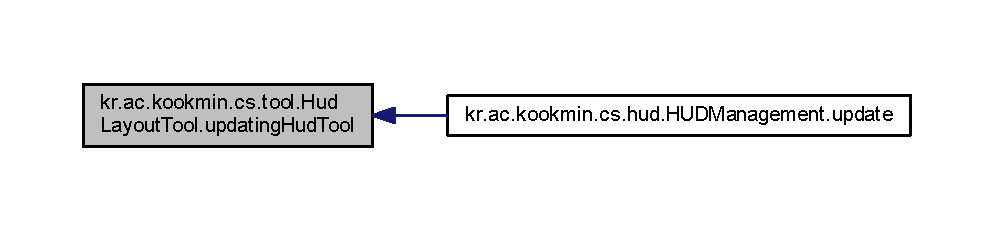
\includegraphics[width=350pt]{classkr_1_1ac_1_1kookmin_1_1cs_1_1tool_1_1_hud_layout_tool_a1206c4b2c371bbbe24cf257492826574_icgraph}
\end{center}
\end{figure}


\hypertarget{classkr_1_1ac_1_1kookmin_1_1cs_1_1tool_1_1_hud_layout_tool_a949f1c99b33700f0d9cd0d7dfbc5c42c}{}\index{kr\+::ac\+::kookmin\+::cs\+::tool\+::\+Hud\+Layout\+Tool@{kr\+::ac\+::kookmin\+::cs\+::tool\+::\+Hud\+Layout\+Tool}!up\+Move\+Offset@{up\+Move\+Offset}}
\index{up\+Move\+Offset@{up\+Move\+Offset}!kr\+::ac\+::kookmin\+::cs\+::tool\+::\+Hud\+Layout\+Tool@{kr\+::ac\+::kookmin\+::cs\+::tool\+::\+Hud\+Layout\+Tool}}
\subsubsection[{up\+Move\+Offset}]{\setlength{\rightskip}{0pt plus 5cm}static void kr.\+ac.\+kookmin.\+cs.\+tool.\+Hud\+Layout\+Tool.\+up\+Move\+Offset (
\begin{DoxyParamCaption}
{}
\end{DoxyParamCaption}
)\hspace{0.3cm}{\ttfamily [static]}}\label{classkr_1_1ac_1_1kookmin_1_1cs_1_1tool_1_1_hud_layout_tool_a949f1c99b33700f0d9cd0d7dfbc5c42c}


This method increases the offset size . 


\begin{DoxyParams}{매개변수}
{\em nothing} & \\
\hline
\end{DoxyParams}
\begin{DoxyReturn}{반환값}
nothing 
\end{DoxyReturn}

\begin{DoxyCode}
286   \{
287     \textcolor{keywordflow}{if}(\hyperlink{classkr_1_1ac_1_1kookmin_1_1cs_1_1tool_1_1_hud_layout_tool_a9207f2feb57881dd1d60896e45408aa5}{moveOffset}==1)
288       \hyperlink{classkr_1_1ac_1_1kookmin_1_1cs_1_1tool_1_1_hud_layout_tool_a9207f2feb57881dd1d60896e45408aa5}{moveOffset}=5;
289     \textcolor{keywordflow}{else} \textcolor{keywordflow}{if}(\hyperlink{classkr_1_1ac_1_1kookmin_1_1cs_1_1tool_1_1_hud_layout_tool_a9207f2feb57881dd1d60896e45408aa5}{moveOffset}==5)
290       \hyperlink{classkr_1_1ac_1_1kookmin_1_1cs_1_1tool_1_1_hud_layout_tool_a9207f2feb57881dd1d60896e45408aa5}{moveOffset}=10;
291     \textcolor{keywordflow}{else} \textcolor{keywordflow}{if}(\hyperlink{classkr_1_1ac_1_1kookmin_1_1cs_1_1tool_1_1_hud_layout_tool_a9207f2feb57881dd1d60896e45408aa5}{moveOffset}==10)
292       \hyperlink{classkr_1_1ac_1_1kookmin_1_1cs_1_1tool_1_1_hud_layout_tool_a9207f2feb57881dd1d60896e45408aa5}{moveOffset}=50;
293     \textcolor{keywordflow}{else}
294       \hyperlink{classkr_1_1ac_1_1kookmin_1_1cs_1_1tool_1_1_hud_layout_tool_a9207f2feb57881dd1d60896e45408aa5}{moveOffset}=100;
295   \}
\end{DoxyCode}


\subsection{멤버 데이타 문서화}
\hypertarget{classkr_1_1ac_1_1kookmin_1_1cs_1_1tool_1_1_hud_layout_tool_a15ae154367e2b7529894488ef358f004}{}\index{kr\+::ac\+::kookmin\+::cs\+::tool\+::\+Hud\+Layout\+Tool@{kr\+::ac\+::kookmin\+::cs\+::tool\+::\+Hud\+Layout\+Tool}!element\+Type@{element\+Type}}
\index{element\+Type@{element\+Type}!kr\+::ac\+::kookmin\+::cs\+::tool\+::\+Hud\+Layout\+Tool@{kr\+::ac\+::kookmin\+::cs\+::tool\+::\+Hud\+Layout\+Tool}}
\subsubsection[{element\+Type}]{\setlength{\rightskip}{0pt plus 5cm}int kr.\+ac.\+kookmin.\+cs.\+tool.\+Hud\+Layout\+Tool.\+element\+Type ={\bf P\+I\+C\+T\+U\+R\+E\+\_\+\+T\+Y\+P\+E}\hspace{0.3cm}{\ttfamily [static]}, {\ttfamily [private]}}\label{classkr_1_1ac_1_1kookmin_1_1cs_1_1tool_1_1_hud_layout_tool_a15ae154367e2b7529894488ef358f004}
\hypertarget{classkr_1_1ac_1_1kookmin_1_1cs_1_1tool_1_1_hud_layout_tool_a92b0ab831e8b62aaebc0974947958349}{}\index{kr\+::ac\+::kookmin\+::cs\+::tool\+::\+Hud\+Layout\+Tool@{kr\+::ac\+::kookmin\+::cs\+::tool\+::\+Hud\+Layout\+Tool}!gui\+Font@{gui\+Font}}
\index{gui\+Font@{gui\+Font}!kr\+::ac\+::kookmin\+::cs\+::tool\+::\+Hud\+Layout\+Tool@{kr\+::ac\+::kookmin\+::cs\+::tool\+::\+Hud\+Layout\+Tool}}
\subsubsection[{gui\+Font}]{\setlength{\rightskip}{0pt plus 5cm}Bitmap\+Font kr.\+ac.\+kookmin.\+cs.\+tool.\+Hud\+Layout\+Tool.\+gui\+Font\hspace{0.3cm}{\ttfamily [static]}, {\ttfamily [private]}}\label{classkr_1_1ac_1_1kookmin_1_1cs_1_1tool_1_1_hud_layout_tool_a92b0ab831e8b62aaebc0974947958349}
\hypertarget{classkr_1_1ac_1_1kookmin_1_1cs_1_1tool_1_1_hud_layout_tool_a1009803f31de3362f409722bb4301dc9}{}\index{kr\+::ac\+::kookmin\+::cs\+::tool\+::\+Hud\+Layout\+Tool@{kr\+::ac\+::kookmin\+::cs\+::tool\+::\+Hud\+Layout\+Tool}!hud\+Frame@{hud\+Frame}}
\index{hud\+Frame@{hud\+Frame}!kr\+::ac\+::kookmin\+::cs\+::tool\+::\+Hud\+Layout\+Tool@{kr\+::ac\+::kookmin\+::cs\+::tool\+::\+Hud\+Layout\+Tool}}
\subsubsection[{hud\+Frame}]{\setlength{\rightskip}{0pt plus 5cm}Node kr.\+ac.\+kookmin.\+cs.\+tool.\+Hud\+Layout\+Tool.\+hud\+Frame\hspace{0.3cm}{\ttfamily [static]}, {\ttfamily [private]}}\label{classkr_1_1ac_1_1kookmin_1_1cs_1_1tool_1_1_hud_layout_tool_a1009803f31de3362f409722bb4301dc9}
\hypertarget{classkr_1_1ac_1_1kookmin_1_1cs_1_1tool_1_1_hud_layout_tool_a48bdb0935f0a1b47acdd97d4ea4adab6}{}\index{kr\+::ac\+::kookmin\+::cs\+::tool\+::\+Hud\+Layout\+Tool@{kr\+::ac\+::kookmin\+::cs\+::tool\+::\+Hud\+Layout\+Tool}!hud\+Tool\+Act\+F@{hud\+Tool\+Act\+F}}
\index{hud\+Tool\+Act\+F@{hud\+Tool\+Act\+F}!kr\+::ac\+::kookmin\+::cs\+::tool\+::\+Hud\+Layout\+Tool@{kr\+::ac\+::kookmin\+::cs\+::tool\+::\+Hud\+Layout\+Tool}}
\subsubsection[{hud\+Tool\+Act\+F}]{\setlength{\rightskip}{0pt plus 5cm}boolean kr.\+ac.\+kookmin.\+cs.\+tool.\+Hud\+Layout\+Tool.\+hud\+Tool\+Act\+F =false\hspace{0.3cm}{\ttfamily [static]}}\label{classkr_1_1ac_1_1kookmin_1_1cs_1_1tool_1_1_hud_layout_tool_a48bdb0935f0a1b47acdd97d4ea4adab6}
\hypertarget{classkr_1_1ac_1_1kookmin_1_1cs_1_1tool_1_1_hud_layout_tool_a6fb0515ee80d878c5fd737b9586772b6}{}\index{kr\+::ac\+::kookmin\+::cs\+::tool\+::\+Hud\+Layout\+Tool@{kr\+::ac\+::kookmin\+::cs\+::tool\+::\+Hud\+Layout\+Tool}!hud\+Tool\+Mode@{hud\+Tool\+Mode}}
\index{hud\+Tool\+Mode@{hud\+Tool\+Mode}!kr\+::ac\+::kookmin\+::cs\+::tool\+::\+Hud\+Layout\+Tool@{kr\+::ac\+::kookmin\+::cs\+::tool\+::\+Hud\+Layout\+Tool}}
\subsubsection[{hud\+Tool\+Mode}]{\setlength{\rightskip}{0pt plus 5cm}int kr.\+ac.\+kookmin.\+cs.\+tool.\+Hud\+Layout\+Tool.\+hud\+Tool\+Mode ={\bf M\+O\+V\+E\+\_\+\+M\+O\+D\+E}\hspace{0.3cm}{\ttfamily [static]}, {\ttfamily [private]}}\label{classkr_1_1ac_1_1kookmin_1_1cs_1_1tool_1_1_hud_layout_tool_a6fb0515ee80d878c5fd737b9586772b6}
\hypertarget{classkr_1_1ac_1_1kookmin_1_1cs_1_1tool_1_1_hud_layout_tool_aecec03baf905df4aaef15cd37abe3abd}{}\index{kr\+::ac\+::kookmin\+::cs\+::tool\+::\+Hud\+Layout\+Tool@{kr\+::ac\+::kookmin\+::cs\+::tool\+::\+Hud\+Layout\+Tool}!M\+O\+V\+E\+\_\+\+M\+O\+D\+E@{M\+O\+V\+E\+\_\+\+M\+O\+D\+E}}
\index{M\+O\+V\+E\+\_\+\+M\+O\+D\+E@{M\+O\+V\+E\+\_\+\+M\+O\+D\+E}!kr\+::ac\+::kookmin\+::cs\+::tool\+::\+Hud\+Layout\+Tool@{kr\+::ac\+::kookmin\+::cs\+::tool\+::\+Hud\+Layout\+Tool}}
\subsubsection[{M\+O\+V\+E\+\_\+\+M\+O\+D\+E}]{\setlength{\rightskip}{0pt plus 5cm}final int kr.\+ac.\+kookmin.\+cs.\+tool.\+Hud\+Layout\+Tool.\+M\+O\+V\+E\+\_\+\+M\+O\+D\+E =10\hspace{0.3cm}{\ttfamily [static]}, {\ttfamily [private]}}\label{classkr_1_1ac_1_1kookmin_1_1cs_1_1tool_1_1_hud_layout_tool_aecec03baf905df4aaef15cd37abe3abd}
\hypertarget{classkr_1_1ac_1_1kookmin_1_1cs_1_1tool_1_1_hud_layout_tool_a9207f2feb57881dd1d60896e45408aa5}{}\index{kr\+::ac\+::kookmin\+::cs\+::tool\+::\+Hud\+Layout\+Tool@{kr\+::ac\+::kookmin\+::cs\+::tool\+::\+Hud\+Layout\+Tool}!move\+Offset@{move\+Offset}}
\index{move\+Offset@{move\+Offset}!kr\+::ac\+::kookmin\+::cs\+::tool\+::\+Hud\+Layout\+Tool@{kr\+::ac\+::kookmin\+::cs\+::tool\+::\+Hud\+Layout\+Tool}}
\subsubsection[{move\+Offset}]{\setlength{\rightskip}{0pt plus 5cm}int kr.\+ac.\+kookmin.\+cs.\+tool.\+Hud\+Layout\+Tool.\+move\+Offset = 50\hspace{0.3cm}{\ttfamily [static]}, {\ttfamily [private]}}\label{classkr_1_1ac_1_1kookmin_1_1cs_1_1tool_1_1_hud_layout_tool_a9207f2feb57881dd1d60896e45408aa5}
\hypertarget{classkr_1_1ac_1_1kookmin_1_1cs_1_1tool_1_1_hud_layout_tool_a614db3c37174dc2724e9a30de2d6a891}{}\index{kr\+::ac\+::kookmin\+::cs\+::tool\+::\+Hud\+Layout\+Tool@{kr\+::ac\+::kookmin\+::cs\+::tool\+::\+Hud\+Layout\+Tool}!move\+Offset\+Text@{move\+Offset\+Text}}
\index{move\+Offset\+Text@{move\+Offset\+Text}!kr\+::ac\+::kookmin\+::cs\+::tool\+::\+Hud\+Layout\+Tool@{kr\+::ac\+::kookmin\+::cs\+::tool\+::\+Hud\+Layout\+Tool}}
\subsubsection[{move\+Offset\+Text}]{\setlength{\rightskip}{0pt plus 5cm}Bitmap\+Text kr.\+ac.\+kookmin.\+cs.\+tool.\+Hud\+Layout\+Tool.\+move\+Offset\+Text\hspace{0.3cm}{\ttfamily [static]}, {\ttfamily [private]}}\label{classkr_1_1ac_1_1kookmin_1_1cs_1_1tool_1_1_hud_layout_tool_a614db3c37174dc2724e9a30de2d6a891}
\hypertarget{classkr_1_1ac_1_1kookmin_1_1cs_1_1tool_1_1_hud_layout_tool_a58687211a1e83d17321e0ee8fc77bd6f}{}\index{kr\+::ac\+::kookmin\+::cs\+::tool\+::\+Hud\+Layout\+Tool@{kr\+::ac\+::kookmin\+::cs\+::tool\+::\+Hud\+Layout\+Tool}!P\+I\+C\+T\+U\+R\+E\+\_\+\+T\+Y\+P\+E@{P\+I\+C\+T\+U\+R\+E\+\_\+\+T\+Y\+P\+E}}
\index{P\+I\+C\+T\+U\+R\+E\+\_\+\+T\+Y\+P\+E@{P\+I\+C\+T\+U\+R\+E\+\_\+\+T\+Y\+P\+E}!kr\+::ac\+::kookmin\+::cs\+::tool\+::\+Hud\+Layout\+Tool@{kr\+::ac\+::kookmin\+::cs\+::tool\+::\+Hud\+Layout\+Tool}}
\subsubsection[{P\+I\+C\+T\+U\+R\+E\+\_\+\+T\+Y\+P\+E}]{\setlength{\rightskip}{0pt plus 5cm}final int kr.\+ac.\+kookmin.\+cs.\+tool.\+Hud\+Layout\+Tool.\+P\+I\+C\+T\+U\+R\+E\+\_\+\+T\+Y\+P\+E =30\hspace{0.3cm}{\ttfamily [static]}, {\ttfamily [private]}}\label{classkr_1_1ac_1_1kookmin_1_1cs_1_1tool_1_1_hud_layout_tool_a58687211a1e83d17321e0ee8fc77bd6f}
\hypertarget{classkr_1_1ac_1_1kookmin_1_1cs_1_1tool_1_1_hud_layout_tool_a8deeda5173478bb396d5eafd48eb5f6f}{}\index{kr\+::ac\+::kookmin\+::cs\+::tool\+::\+Hud\+Layout\+Tool@{kr\+::ac\+::kookmin\+::cs\+::tool\+::\+Hud\+Layout\+Tool}!picture\+Info\+List@{picture\+Info\+List}}
\index{picture\+Info\+List@{picture\+Info\+List}!kr\+::ac\+::kookmin\+::cs\+::tool\+::\+Hud\+Layout\+Tool@{kr\+::ac\+::kookmin\+::cs\+::tool\+::\+Hud\+Layout\+Tool}}
\subsubsection[{picture\+Info\+List}]{\setlength{\rightskip}{0pt plus 5cm}Array\+List$<$Picture\+Info$>$ kr.\+ac.\+kookmin.\+cs.\+tool.\+Hud\+Layout\+Tool.\+picture\+Info\+List =new Array\+List$<$Picture\+Info$>$()\hspace{0.3cm}{\ttfamily [static]}, {\ttfamily [private]}}\label{classkr_1_1ac_1_1kookmin_1_1cs_1_1tool_1_1_hud_layout_tool_a8deeda5173478bb396d5eafd48eb5f6f}
\hypertarget{classkr_1_1ac_1_1kookmin_1_1cs_1_1tool_1_1_hud_layout_tool_acbd0f26c3534561b74d5f3b75ae4d622}{}\index{kr\+::ac\+::kookmin\+::cs\+::tool\+::\+Hud\+Layout\+Tool@{kr\+::ac\+::kookmin\+::cs\+::tool\+::\+Hud\+Layout\+Tool}!picture\+List@{picture\+List}}
\index{picture\+List@{picture\+List}!kr\+::ac\+::kookmin\+::cs\+::tool\+::\+Hud\+Layout\+Tool@{kr\+::ac\+::kookmin\+::cs\+::tool\+::\+Hud\+Layout\+Tool}}
\subsubsection[{picture\+List}]{\setlength{\rightskip}{0pt plus 5cm}Array\+List$<$Picture$>$ kr.\+ac.\+kookmin.\+cs.\+tool.\+Hud\+Layout\+Tool.\+picture\+List =new Array\+List$<$Picture$>$()\hspace{0.3cm}{\ttfamily [static]}, {\ttfamily [private]}}\label{classkr_1_1ac_1_1kookmin_1_1cs_1_1tool_1_1_hud_layout_tool_acbd0f26c3534561b74d5f3b75ae4d622}
\hypertarget{classkr_1_1ac_1_1kookmin_1_1cs_1_1tool_1_1_hud_layout_tool_a1611225d44b7a53cd3a3dcf3dc85b784}{}\index{kr\+::ac\+::kookmin\+::cs\+::tool\+::\+Hud\+Layout\+Tool@{kr\+::ac\+::kookmin\+::cs\+::tool\+::\+Hud\+Layout\+Tool}!present\+Element\+Ind@{present\+Element\+Ind}}
\index{present\+Element\+Ind@{present\+Element\+Ind}!kr\+::ac\+::kookmin\+::cs\+::tool\+::\+Hud\+Layout\+Tool@{kr\+::ac\+::kookmin\+::cs\+::tool\+::\+Hud\+Layout\+Tool}}
\subsubsection[{present\+Element\+Ind}]{\setlength{\rightskip}{0pt plus 5cm}int kr.\+ac.\+kookmin.\+cs.\+tool.\+Hud\+Layout\+Tool.\+present\+Element\+Ind = 0\hspace{0.3cm}{\ttfamily [static]}, {\ttfamily [private]}}\label{classkr_1_1ac_1_1kookmin_1_1cs_1_1tool_1_1_hud_layout_tool_a1611225d44b7a53cd3a3dcf3dc85b784}
\hypertarget{classkr_1_1ac_1_1kookmin_1_1cs_1_1tool_1_1_hud_layout_tool_ae849face952e72f68da8d09981c71c43}{}\index{kr\+::ac\+::kookmin\+::cs\+::tool\+::\+Hud\+Layout\+Tool@{kr\+::ac\+::kookmin\+::cs\+::tool\+::\+Hud\+Layout\+Tool}!present\+Text\+Ind@{present\+Text\+Ind}}
\index{present\+Text\+Ind@{present\+Text\+Ind}!kr\+::ac\+::kookmin\+::cs\+::tool\+::\+Hud\+Layout\+Tool@{kr\+::ac\+::kookmin\+::cs\+::tool\+::\+Hud\+Layout\+Tool}}
\subsubsection[{present\+Text\+Ind}]{\setlength{\rightskip}{0pt plus 5cm}int kr.\+ac.\+kookmin.\+cs.\+tool.\+Hud\+Layout\+Tool.\+present\+Text\+Ind =0\hspace{0.3cm}{\ttfamily [static]}, {\ttfamily [private]}}\label{classkr_1_1ac_1_1kookmin_1_1cs_1_1tool_1_1_hud_layout_tool_ae849face952e72f68da8d09981c71c43}
\hypertarget{classkr_1_1ac_1_1kookmin_1_1cs_1_1tool_1_1_hud_layout_tool_af06a05d18241dcbe2bc4f2c96d157ee0}{}\index{kr\+::ac\+::kookmin\+::cs\+::tool\+::\+Hud\+Layout\+Tool@{kr\+::ac\+::kookmin\+::cs\+::tool\+::\+Hud\+Layout\+Tool}!sim@{sim}}
\index{sim@{sim}!kr\+::ac\+::kookmin\+::cs\+::tool\+::\+Hud\+Layout\+Tool@{kr\+::ac\+::kookmin\+::cs\+::tool\+::\+Hud\+Layout\+Tool}}
\subsubsection[{sim}]{\setlength{\rightskip}{0pt plus 5cm}Simulation\+Basics kr.\+ac.\+kookmin.\+cs.\+tool.\+Hud\+Layout\+Tool.\+sim\hspace{0.3cm}{\ttfamily [static]}, {\ttfamily [private]}}\label{classkr_1_1ac_1_1kookmin_1_1cs_1_1tool_1_1_hud_layout_tool_af06a05d18241dcbe2bc4f2c96d157ee0}
\hypertarget{classkr_1_1ac_1_1kookmin_1_1cs_1_1tool_1_1_hud_layout_tool_a7072db948603a28712cb20279dc44a3a}{}\index{kr\+::ac\+::kookmin\+::cs\+::tool\+::\+Hud\+Layout\+Tool@{kr\+::ac\+::kookmin\+::cs\+::tool\+::\+Hud\+Layout\+Tool}!S\+I\+Z\+E\+\_\+\+M\+O\+D\+E@{S\+I\+Z\+E\+\_\+\+M\+O\+D\+E}}
\index{S\+I\+Z\+E\+\_\+\+M\+O\+D\+E@{S\+I\+Z\+E\+\_\+\+M\+O\+D\+E}!kr\+::ac\+::kookmin\+::cs\+::tool\+::\+Hud\+Layout\+Tool@{kr\+::ac\+::kookmin\+::cs\+::tool\+::\+Hud\+Layout\+Tool}}
\subsubsection[{S\+I\+Z\+E\+\_\+\+M\+O\+D\+E}]{\setlength{\rightskip}{0pt plus 5cm}final int kr.\+ac.\+kookmin.\+cs.\+tool.\+Hud\+Layout\+Tool.\+S\+I\+Z\+E\+\_\+\+M\+O\+D\+E =20\hspace{0.3cm}{\ttfamily [static]}, {\ttfamily [private]}}\label{classkr_1_1ac_1_1kookmin_1_1cs_1_1tool_1_1_hud_layout_tool_a7072db948603a28712cb20279dc44a3a}
\hypertarget{classkr_1_1ac_1_1kookmin_1_1cs_1_1tool_1_1_hud_layout_tool_abbd7ff0bb5a36036d96b889922951fd9}{}\index{kr\+::ac\+::kookmin\+::cs\+::tool\+::\+Hud\+Layout\+Tool@{kr\+::ac\+::kookmin\+::cs\+::tool\+::\+Hud\+Layout\+Tool}!T\+E\+X\+T\+\_\+\+T\+Y\+P\+E@{T\+E\+X\+T\+\_\+\+T\+Y\+P\+E}}
\index{T\+E\+X\+T\+\_\+\+T\+Y\+P\+E@{T\+E\+X\+T\+\_\+\+T\+Y\+P\+E}!kr\+::ac\+::kookmin\+::cs\+::tool\+::\+Hud\+Layout\+Tool@{kr\+::ac\+::kookmin\+::cs\+::tool\+::\+Hud\+Layout\+Tool}}
\subsubsection[{T\+E\+X\+T\+\_\+\+T\+Y\+P\+E}]{\setlength{\rightskip}{0pt plus 5cm}final int kr.\+ac.\+kookmin.\+cs.\+tool.\+Hud\+Layout\+Tool.\+T\+E\+X\+T\+\_\+\+T\+Y\+P\+E =40\hspace{0.3cm}{\ttfamily [static]}, {\ttfamily [private]}}\label{classkr_1_1ac_1_1kookmin_1_1cs_1_1tool_1_1_hud_layout_tool_abbd7ff0bb5a36036d96b889922951fd9}
\hypertarget{classkr_1_1ac_1_1kookmin_1_1cs_1_1tool_1_1_hud_layout_tool_a028d96b28a4f07007430d9ac3d29eac9}{}\index{kr\+::ac\+::kookmin\+::cs\+::tool\+::\+Hud\+Layout\+Tool@{kr\+::ac\+::kookmin\+::cs\+::tool\+::\+Hud\+Layout\+Tool}!text\+Info\+List@{text\+Info\+List}}
\index{text\+Info\+List@{text\+Info\+List}!kr\+::ac\+::kookmin\+::cs\+::tool\+::\+Hud\+Layout\+Tool@{kr\+::ac\+::kookmin\+::cs\+::tool\+::\+Hud\+Layout\+Tool}}
\subsubsection[{text\+Info\+List}]{\setlength{\rightskip}{0pt plus 5cm}Array\+List$<$Bitmap\+Text\+Info$>$ kr.\+ac.\+kookmin.\+cs.\+tool.\+Hud\+Layout\+Tool.\+text\+Info\+List =new Array\+List$<$Bitmap\+Text\+Info$>$()\hspace{0.3cm}{\ttfamily [static]}, {\ttfamily [private]}}\label{classkr_1_1ac_1_1kookmin_1_1cs_1_1tool_1_1_hud_layout_tool_a028d96b28a4f07007430d9ac3d29eac9}
\hypertarget{classkr_1_1ac_1_1kookmin_1_1cs_1_1tool_1_1_hud_layout_tool_a494376a3549ec46802ef2de1ebf10bc1}{}\index{kr\+::ac\+::kookmin\+::cs\+::tool\+::\+Hud\+Layout\+Tool@{kr\+::ac\+::kookmin\+::cs\+::tool\+::\+Hud\+Layout\+Tool}!text\+List@{text\+List}}
\index{text\+List@{text\+List}!kr\+::ac\+::kookmin\+::cs\+::tool\+::\+Hud\+Layout\+Tool@{kr\+::ac\+::kookmin\+::cs\+::tool\+::\+Hud\+Layout\+Tool}}
\subsubsection[{text\+List}]{\setlength{\rightskip}{0pt plus 5cm}Array\+List$<$Bitmap\+Text$>$ kr.\+ac.\+kookmin.\+cs.\+tool.\+Hud\+Layout\+Tool.\+text\+List =new Array\+List$<$Bitmap\+Text$>$()\hspace{0.3cm}{\ttfamily [static]}, {\ttfamily [private]}}\label{classkr_1_1ac_1_1kookmin_1_1cs_1_1tool_1_1_hud_layout_tool_a494376a3549ec46802ef2de1ebf10bc1}


이 클래스에 대한 문서화 페이지는 다음의 파일로부터 생성되었습니다.\+:\begin{DoxyCompactItemize}
\item 
C\+:/\+Users/\+Karasion/git/\+Capstone2015-\/\+Purple\+Ocean/src/kr/ac/kookmin/cs/tool/\hyperlink{_hud_layout_tool_8java}{Hud\+Layout\+Tool.\+java}\end{DoxyCompactItemize}

\hypertarget{classkr_1_1ac_1_1kookmin_1_1cs_1_1hud_1_1_h_u_d_management}{}\section{kr.\+ac.\+kookmin.\+cs.\+hud.\+H\+U\+D\+Management 클래스 참조}
\label{classkr_1_1ac_1_1kookmin_1_1cs_1_1hud_1_1_h_u_d_management}\index{kr.\+ac.\+kookmin.\+cs.\+hud.\+H\+U\+D\+Management@{kr.\+ac.\+kookmin.\+cs.\+hud.\+H\+U\+D\+Management}}


Class that manages the functions of the H\+U\+D panel.  




kr.\+ac.\+kookmin.\+cs.\+hud.\+H\+U\+D\+Management에 대한 협력 다이어그램\+:\nopagebreak
\begin{figure}[H]
\begin{center}
\leavevmode
\includegraphics[width=350pt]{classkr_1_1ac_1_1kookmin_1_1cs_1_1hud_1_1_h_u_d_management__coll__graph}
\end{center}
\end{figure}
\subsection*{정적 Public 멤버 함수}
\begin{DoxyCompactItemize}
\item 
static void \hyperlink{classkr_1_1ac_1_1kookmin_1_1cs_1_1hud_1_1_h_u_d_management_a09bdb891071027c0834bb5e300dbd530}{init} (Simulator simulator)
\begin{DoxyCompactList}\small\item\em Method to initialize the basic H\+U\+D element and H\+U\+D layout class element. \end{DoxyCompactList}\item 
static void \hyperlink{classkr_1_1ac_1_1kookmin_1_1cs_1_1hud_1_1_h_u_d_management_a0aa136c1c12cdff5b49304a0b750d3bb}{update} ()
\begin{DoxyCompactList}\small\item\em Method to update the state of the H\+U\+D in real time. \end{DoxyCompactList}\item 
static void \hyperlink{classkr_1_1ac_1_1kookmin_1_1cs_1_1hud_1_1_h_u_d_management_aa5add7f6fd1b0015e8b55a5e1edbd9e0}{hud\+Attach} ()
\begin{DoxyCompactList}\small\item\em Method to add the main screen of H\+U\+D to H\+U\+D panel. \end{DoxyCompactList}\item 
static void \hyperlink{classkr_1_1ac_1_1kookmin_1_1cs_1_1hud_1_1_h_u_d_management_aebd2c1a29ca7f1ccc3002126f6386f9e}{hud\+Detach} ()
\begin{DoxyCompactList}\small\item\em Method to delete H\+U\+D to H\+U\+D panel. \end{DoxyCompactList}\item 
static void \hyperlink{classkr_1_1ac_1_1kookmin_1_1cs_1_1hud_1_1_h_u_d_management_aa3589b792b8862b3a04c58a6eb52ea23}{backup\+H\+U\+D} (int change\+State)
\begin{DoxyCompactList}\small\item\em Method to back up the previous state of H\+U\+D. \end{DoxyCompactList}\item 
static int \hyperlink{classkr_1_1ac_1_1kookmin_1_1cs_1_1hud_1_1_h_u_d_management_a946946e34bd696cf5d51c9d7bd2da38e}{restore\+H\+U\+D} ()
\begin{DoxyCompactList}\small\item\em Method to return the state of H\+U\+D to a previous state. \end{DoxyCompactList}\item 
static boolean \hyperlink{classkr_1_1ac_1_1kookmin_1_1cs_1_1hud_1_1_h_u_d_management_acaf22b9e65e755c7504cf7d58b4e61c5}{is\+Camera\+Ego} ()
\item 
static void \hyperlink{classkr_1_1ac_1_1kookmin_1_1cs_1_1hud_1_1_h_u_d_management_ab216b1d334e23a1eac3b2ba468f420da}{set\+Camera\+Ego} (boolean flag)
\item 
static void \hyperlink{classkr_1_1ac_1_1kookmin_1_1cs_1_1hud_1_1_h_u_d_management_aee0e46bbcf6e6db490490c48fc32498a}{key\+Flag\+Setting} ()
\begin{DoxyCompactList}\small\item\em Method to set whether the press and hold the H\+U\+D key. \end{DoxyCompactList}\item 
static void \hyperlink{classkr_1_1ac_1_1kookmin_1_1cs_1_1hud_1_1_h_u_d_management_ae9d4e81f2a9e51e0269f80d6c0b192ff}{set\+Navi\+Type} (String navi\+Type, String distance)
\begin{DoxyCompactList}\small\item\em Method for setting the direction of navigation and the rest of the distance . \end{DoxyCompactList}\item 
static boolean \hyperlink{classkr_1_1ac_1_1kookmin_1_1cs_1_1hud_1_1_h_u_d_management_ae13f71ba28cbace432c6991b05e3389b}{get\+Key\+Flag} ()
\item 
static int \hyperlink{classkr_1_1ac_1_1kookmin_1_1cs_1_1hud_1_1_h_u_d_management_ae53c044c1e3f19918e4594266629f4cf}{get\+State} ()
\item 
static void \hyperlink{classkr_1_1ac_1_1kookmin_1_1cs_1_1hud_1_1_h_u_d_management_a03e741a1bf315bb7cccc881479731038}{left\+Move\+Cursor} ()
\begin{DoxyCompactList}\small\item\em Method to move the cursor of H\+U\+D menu on the left. \end{DoxyCompactList}\item 
static void \hyperlink{classkr_1_1ac_1_1kookmin_1_1cs_1_1hud_1_1_h_u_d_management_abaa831b57d11f6e159917476881112e1}{right\+Move\+Cursor} ()
\begin{DoxyCompactList}\small\item\em Method to move the cursor of H\+U\+D menu on the right. \end{DoxyCompactList}\item 
static void \hyperlink{classkr_1_1ac_1_1kookmin_1_1cs_1_1hud_1_1_h_u_d_management_a454c18c087d019b055fda4a631720819}{select\+Menu} ()
\begin{DoxyCompactList}\small\item\em Method to run the registered function in H\+U\+D menu. \end{DoxyCompactList}\item 
static void \hyperlink{classkr_1_1ac_1_1kookmin_1_1cs_1_1hud_1_1_h_u_d_management_af46086e2dbfc7fe58b45bc5d98fe08d8}{escape\+Menu} ()
\begin{DoxyCompactList}\small\item\em Method to get out from the menu function running. \end{DoxyCompactList}\item 
static void \hyperlink{classkr_1_1ac_1_1kookmin_1_1cs_1_1hud_1_1_h_u_d_management_a88d77a9d61e931e5b8460e7bfaa9558f}{disable\+Menu} (int state)
\begin{DoxyCompactList}\small\item\em This Method is to disable the menu icon. \end{DoxyCompactList}\item 
static void \hyperlink{classkr_1_1ac_1_1kookmin_1_1cs_1_1hud_1_1_h_u_d_management_a2d3e988e5636714778382ba504e00c6e}{enable\+Menu} ()
\begin{DoxyCompactList}\small\item\em This Method is to enable the menu icon. \end{DoxyCompactList}\item 
static void \hyperlink{classkr_1_1ac_1_1kookmin_1_1cs_1_1hud_1_1_h_u_d_management_a57652e0e587a00547e4664e13e87453d}{attach} (Node sub\+Gui)
\begin{DoxyCompactList}\small\item\em The Method is the ability to attach the H\+U\+D layout to the panel . \end{DoxyCompactList}\item 
static void \hyperlink{classkr_1_1ac_1_1kookmin_1_1cs_1_1hud_1_1_h_u_d_management_aa447140a88b6a509cf0c88518972ceb6}{detach} (Node sub\+Gui)
\begin{DoxyCompactList}\small\item\em The Method is the ability to detach the H\+U\+D layout to the panel . \end{DoxyCompactList}\item 
static int \hyperlink{classkr_1_1ac_1_1kookmin_1_1cs_1_1hud_1_1_h_u_d_management_a7b83ede582afefb75bfe90ed3c8fd688}{regist} (\hyperlink{classkr_1_1ac_1_1kookmin_1_1cs_1_1hud_1_1_h_u_d_class_template}{H\+U\+D\+Class\+Template} \hyperlink{classkr_1_1ac_1_1kookmin_1_1cs_1_1hud_1_1_h_u_d_management_a4c4a440b9bdbbe24eb50ee79826aee53}{hud})
\begin{DoxyCompactList}\small\item\em The Method is a function of registering the H\+U\+D layout class to \hyperlink{classkr_1_1ac_1_1kookmin_1_1cs_1_1hud_1_1_h_u_d_management}{H\+U\+D\+Management}. \end{DoxyCompactList}\item 
static void \hyperlink{classkr_1_1ac_1_1kookmin_1_1cs_1_1hud_1_1_h_u_d_management_af8454651113100e20b4134f4bae1ea8e}{set\+Menu\+Icon} (Picture pic\+\_\+en, Picture pic\+\_\+dis, int state)
\begin{DoxyCompactList}\small\item\em The Method is a function of add the icon of H\+U\+D menu bar. \end{DoxyCompactList}\item 
static void \hyperlink{classkr_1_1ac_1_1kookmin_1_1cs_1_1hud_1_1_h_u_d_management_ae06e3a800da57cd4d85308ea6252617b}{left\+Key\+Act} ()
\begin{DoxyCompactList}\small\item\em This method is to map the action of the key. \end{DoxyCompactList}\item 
static void \hyperlink{classkr_1_1ac_1_1kookmin_1_1cs_1_1hud_1_1_h_u_d_management_aace7213b80851272394174ac9dc20f54}{right\+Key\+Act} ()
\begin{DoxyCompactList}\small\item\em This method is to map the action of the key. \end{DoxyCompactList}\item 
static void \hyperlink{classkr_1_1ac_1_1kookmin_1_1cs_1_1hud_1_1_h_u_d_management_a02236b52bb21cdc0b8d2408463c0a879}{up\+Key\+Act} ()
\begin{DoxyCompactList}\small\item\em This method is to map the action of the key. \end{DoxyCompactList}\item 
static void \hyperlink{classkr_1_1ac_1_1kookmin_1_1cs_1_1hud_1_1_h_u_d_management_ac1f57a7a1a845c100ef9f0edaa9167fe}{down\+Key\+Act} ()
\begin{DoxyCompactList}\small\item\em This method is to map the action of the key. \end{DoxyCompactList}\item 
static void \hyperlink{classkr_1_1ac_1_1kookmin_1_1cs_1_1hud_1_1_h_u_d_management_af416f945909ff83db9206403417e93c6}{push\+Key\+Act} ()
\begin{DoxyCompactList}\small\item\em This method is to map the action of the key. \end{DoxyCompactList}\end{DoxyCompactItemize}
\subsection*{정적 Public 속성}
\begin{DoxyCompactItemize}
\item 
static final int \hyperlink{classkr_1_1ac_1_1kookmin_1_1cs_1_1hud_1_1_h_u_d_management_aed0bc1b7b1fd78bb588e2321b44cb254}{N\+O\+N\+\_\+\+S\+T\+A\+T\+E} = -\/1
\end{DoxyCompactItemize}
\subsection*{정적 Private 멤버 함수}
\begin{DoxyCompactItemize}
\item 
static void \hyperlink{classkr_1_1ac_1_1kookmin_1_1cs_1_1hud_1_1_h_u_d_management_ae556ec9b1e304f6b7ac343d19186b31e}{hud\+Menu\+Init} ()
\begin{DoxyCompactList}\small\item\em Method to set the position of the H\+U\+D menu icon. \end{DoxyCompactList}\item 
static void \hyperlink{classkr_1_1ac_1_1kookmin_1_1cs_1_1hud_1_1_h_u_d_management_aeb454637f977e672b79282823b6b1cde}{update\+Current\+Speed\+Text} (Car car)
\begin{DoxyCompactList}\small\item\em Method to read the current speed value in Opend\+D\+S for H\+U\+D speed display function. \end{DoxyCompactList}\item 
static void \hyperlink{classkr_1_1ac_1_1kookmin_1_1cs_1_1hud_1_1_h_u_d_management_ae4cd0a7adf3e6e05e2c515bc4ec630ac}{update\+Navigator\+Sign} ()
\begin{DoxyCompactList}\small\item\em Method to update the direction of navigation. \end{DoxyCompactList}\item 
static void \hyperlink{classkr_1_1ac_1_1kookmin_1_1cs_1_1hud_1_1_h_u_d_management_a17e1d7f91f4334de06399c149d455781}{default\+Function\+Attach} ()
\begin{DoxyCompactList}\small\item\em Method to add a H\+U\+D basic functions in H\+U\+D panel. \end{DoxyCompactList}\end{DoxyCompactItemize}
\subsection*{정적 Private 속성}
\begin{DoxyCompactItemize}
\item 
static Simulation\+Basics \hyperlink{classkr_1_1ac_1_1kookmin_1_1cs_1_1hud_1_1_h_u_d_management_abcbcea66aba5169a6d07c407d1e3c86d}{sim}
\item 
static boolean \hyperlink{classkr_1_1ac_1_1kookmin_1_1cs_1_1hud_1_1_h_u_d_management_ae9746ce389f6ae79a1f245943631e8af}{ego\+Flag} = false
\item 
static boolean \hyperlink{classkr_1_1ac_1_1kookmin_1_1cs_1_1hud_1_1_h_u_d_management_ac411b7fde47d1bec2bd043b2f2df51e8}{key\+On} =false
\item 
static Node \hyperlink{classkr_1_1ac_1_1kookmin_1_1cs_1_1hud_1_1_h_u_d_management_af523238fd17953e526bc0d81a4057ebc}{node\+Gui}
\item 
static Node \hyperlink{classkr_1_1ac_1_1kookmin_1_1cs_1_1hud_1_1_h_u_d_management_a4c4a440b9bdbbe24eb50ee79826aee53}{hud}
\item 
static Node \hyperlink{classkr_1_1ac_1_1kookmin_1_1cs_1_1hud_1_1_h_u_d_management_a42b564e79a47075337594ae2a83f4309}{hud\+Menu}
\item 
static Bitmap\+Text \hyperlink{classkr_1_1ac_1_1kookmin_1_1cs_1_1hud_1_1_h_u_d_management_afd73165355cc807a706c8e5c29a3f271}{current\+Speed\+Text}
\item 
static Bitmap\+Text \hyperlink{classkr_1_1ac_1_1kookmin_1_1cs_1_1hud_1_1_h_u_d_management_a462366543dcc71453006bd2ded4e463a}{distance\+Text}
\item 
static Picture \hyperlink{classkr_1_1ac_1_1kookmin_1_1cs_1_1hud_1_1_h_u_d_management_a5a7a9b54b80a068feadce31902fca2ab}{navigator\+Sign}
\item 
static int \hyperlink{classkr_1_1ac_1_1kookmin_1_1cs_1_1hud_1_1_h_u_d_management_a6e135a288ebdc4381eb971ab03d0bd6e}{current\+State} = \hyperlink{classkr_1_1ac_1_1kookmin_1_1cs_1_1hud_1_1_h_u_d_management_aed0bc1b7b1fd78bb588e2321b44cb254}{N\+O\+N\+\_\+\+S\+T\+A\+T\+E}
\item 
static int \hyperlink{classkr_1_1ac_1_1kookmin_1_1cs_1_1hud_1_1_h_u_d_management_ac951218e3771940c9b4555f3ac830d7f}{state\+Num} = 0
\item 
static Array\+List$<$ \hyperlink{classkr_1_1ac_1_1kookmin_1_1cs_1_1hud_1_1_h_u_d_class_template}{H\+U\+D\+Class\+Template} $>$ \hyperlink{classkr_1_1ac_1_1kookmin_1_1cs_1_1hud_1_1_h_u_d_management_a9eec206ae0d3464de9e92243ae0aba24}{hud\+List} = new Array\+List$<$\hyperlink{classkr_1_1ac_1_1kookmin_1_1cs_1_1hud_1_1_h_u_d_class_template}{H\+U\+D\+Class\+Template}$>$()
\item 
static int\mbox{[}$\,$\mbox{]} \hyperlink{classkr_1_1ac_1_1kookmin_1_1cs_1_1hud_1_1_h_u_d_management_a2e980ba0f951c11c7b41190197f138fb}{backup\+State} = new int\mbox{[}10\mbox{]}
\item 
static int \hyperlink{classkr_1_1ac_1_1kookmin_1_1cs_1_1hud_1_1_h_u_d_management_a4d8dcd83fa46fb810848d39518bd2a89}{backup\+Cnt} = 0
\item 
static int\mbox{[}$\,$\mbox{]} \hyperlink{classkr_1_1ac_1_1kookmin_1_1cs_1_1hud_1_1_h_u_d_management_a1f856e5328f0219dbb586c5297b6b62b}{menu\+State} = new int\mbox{[}5\mbox{]}
\item 
static int \hyperlink{classkr_1_1ac_1_1kookmin_1_1cs_1_1hud_1_1_h_u_d_management_a3a60a8d9a72d5d242796fdaa9c76905d}{x}
\item 
static int\mbox{[}$\,$\mbox{]} \hyperlink{classkr_1_1ac_1_1kookmin_1_1cs_1_1hud_1_1_h_u_d_management_a56a670048b3af508378ccfaab214893e}{menubar\+Pos\+X} = new int\mbox{[}5\mbox{]}
\item 
static int \hyperlink{classkr_1_1ac_1_1kookmin_1_1cs_1_1hud_1_1_h_u_d_management_a642380be5c9dd050a5678665b2c2e2fa}{menubar\+Pos\+Y}
\item 
static int\mbox{[}$\,$\mbox{]} \hyperlink{classkr_1_1ac_1_1kookmin_1_1cs_1_1hud_1_1_h_u_d_management_a62b6b5ec5cb0eae74acaacccd2c3bee6}{cursor\+Pos\+X} = new int\mbox{[}5\mbox{]}
\item 
static int \hyperlink{classkr_1_1ac_1_1kookmin_1_1cs_1_1hud_1_1_h_u_d_management_a1bc74f45485b6a429e54e8be6a66b6b1}{cursor\+Pos\+Y}
\item 
static int \hyperlink{classkr_1_1ac_1_1kookmin_1_1cs_1_1hud_1_1_h_u_d_management_ab9d252f0b80e76c4930b8e0fd288f019}{menu\+Start\+Index}
\item 
static int \hyperlink{classkr_1_1ac_1_1kookmin_1_1cs_1_1hud_1_1_h_u_d_management_aa53116bd342eeee2ab96d1edabf5561d}{menu\+End\+Index}
\item 
static int \hyperlink{classkr_1_1ac_1_1kookmin_1_1cs_1_1hud_1_1_h_u_d_management_af69baaadf8bdb8b4f429269357fb84d9}{menu\+Num} = 0
\item 
static int \hyperlink{classkr_1_1ac_1_1kookmin_1_1cs_1_1hud_1_1_h_u_d_management_a138d02aacf241cd6234acfc9512f78aa}{cursor\+Pos} = 0
\item 
static Picture\mbox{[}$\,$\mbox{]} \hyperlink{classkr_1_1ac_1_1kookmin_1_1cs_1_1hud_1_1_h_u_d_management_accf7a9ec5092e5872460755f3b81d6d5}{pic\+Arry\+Menu\+En} = new Picture\mbox{[}5\mbox{]}
\item 
static Picture\mbox{[}$\,$\mbox{]} \hyperlink{classkr_1_1ac_1_1kookmin_1_1cs_1_1hud_1_1_h_u_d_management_ab5d064aafc8e948ecd818cfec7acbb3c}{pic\+Arry\+Menu\+Dis} = new Picture\mbox{[}5\mbox{]}
\item 
static Picture \hyperlink{classkr_1_1ac_1_1kookmin_1_1cs_1_1hud_1_1_h_u_d_management_a8bd64fe62e6e91c9bd83a274eb59faa9}{cursor\+Icon}
\item 
static final int \hyperlink{classkr_1_1ac_1_1kookmin_1_1cs_1_1hud_1_1_h_u_d_management_aea6d53b87b47693e0d365f8cd6fba75f}{M\+E\+N\+U\+\_\+\+A\+L\+L} = -\/1
\item 
static final int \hyperlink{classkr_1_1ac_1_1kookmin_1_1cs_1_1hud_1_1_h_u_d_management_a3945824c1d285a532b81075debe3a8cf}{M\+E\+N\+U\+\_\+\+P\+O\+S1} = 0
\item 
static final int \hyperlink{classkr_1_1ac_1_1kookmin_1_1cs_1_1hud_1_1_h_u_d_management_a2543a9a44db444550bd334d354616928}{M\+E\+N\+U\+\_\+\+P\+O\+S2} = 1
\item 
static final int \hyperlink{classkr_1_1ac_1_1kookmin_1_1cs_1_1hud_1_1_h_u_d_management_a79ee86a5edf36a3cd5f9c9d75e40d9db}{M\+E\+N\+U\+\_\+\+P\+O\+S3} = 2
\item 
static final int \hyperlink{classkr_1_1ac_1_1kookmin_1_1cs_1_1hud_1_1_h_u_d_management_a6cae012a8c111a62d031ec590afe56bb}{M\+E\+N\+U\+\_\+\+P\+O\+S4} = 3
\item 
static final int \hyperlink{classkr_1_1ac_1_1kookmin_1_1cs_1_1hud_1_1_h_u_d_management_abfc1e4fd6ea23ecf49abfb86d47af051}{M\+E\+N\+U\+\_\+\+P\+O\+S5} = 4
\end{DoxyCompactItemize}


\subsection{상세한 설명}
Class that manages the functions of the H\+U\+D panel. 

This class manages the functions by state separately divided , it serves to provide an A\+P\+I related functions to be used externally \begin{DoxyAuthor}{작성자}
Jo-\/kwanghyeon, Im-\/gisung 
\end{DoxyAuthor}


\subsection{멤버 함수 문서화}
\hypertarget{classkr_1_1ac_1_1kookmin_1_1cs_1_1hud_1_1_h_u_d_management_a57652e0e587a00547e4664e13e87453d}{}\index{kr\+::ac\+::kookmin\+::cs\+::hud\+::\+H\+U\+D\+Management@{kr\+::ac\+::kookmin\+::cs\+::hud\+::\+H\+U\+D\+Management}!attach@{attach}}
\index{attach@{attach}!kr\+::ac\+::kookmin\+::cs\+::hud\+::\+H\+U\+D\+Management@{kr\+::ac\+::kookmin\+::cs\+::hud\+::\+H\+U\+D\+Management}}
\subsubsection[{attach}]{\setlength{\rightskip}{0pt plus 5cm}static void kr.\+ac.\+kookmin.\+cs.\+hud.\+H\+U\+D\+Management.\+attach (
\begin{DoxyParamCaption}
\item[{Node}]{sub\+Gui}
\end{DoxyParamCaption}
)\hspace{0.3cm}{\ttfamily [static]}}\label{classkr_1_1ac_1_1kookmin_1_1cs_1_1hud_1_1_h_u_d_management_a57652e0e587a00547e4664e13e87453d}


The Method is the ability to attach the H\+U\+D layout to the panel . 


\begin{DoxyParams}{매개변수}
{\em Node} & argument sub\+Gui \\
\hline
\end{DoxyParams}
\begin{DoxyReturn}{반환값}
Nothing 
\end{DoxyReturn}

\begin{DoxyCode}
616   \{
617     \hyperlink{classkr_1_1ac_1_1kookmin_1_1cs_1_1hud_1_1_h_u_d_management_a4c4a440b9bdbbe24eb50ee79826aee53}{hud}.attachChild(subGui);
618   \}
\end{DoxyCode}


이 함수를 호출하는 함수들에 대한 그래프입니다.\+:\nopagebreak
\begin{figure}[H]
\begin{center}
\leavevmode
\includegraphics[width=350pt]{classkr_1_1ac_1_1kookmin_1_1cs_1_1hud_1_1_h_u_d_management_a57652e0e587a00547e4664e13e87453d_icgraph}
\end{center}
\end{figure}


\hypertarget{classkr_1_1ac_1_1kookmin_1_1cs_1_1hud_1_1_h_u_d_management_aa3589b792b8862b3a04c58a6eb52ea23}{}\index{kr\+::ac\+::kookmin\+::cs\+::hud\+::\+H\+U\+D\+Management@{kr\+::ac\+::kookmin\+::cs\+::hud\+::\+H\+U\+D\+Management}!backup\+H\+U\+D@{backup\+H\+U\+D}}
\index{backup\+H\+U\+D@{backup\+H\+U\+D}!kr\+::ac\+::kookmin\+::cs\+::hud\+::\+H\+U\+D\+Management@{kr\+::ac\+::kookmin\+::cs\+::hud\+::\+H\+U\+D\+Management}}
\subsubsection[{backup\+H\+U\+D}]{\setlength{\rightskip}{0pt plus 5cm}static void kr.\+ac.\+kookmin.\+cs.\+hud.\+H\+U\+D\+Management.\+backup\+H\+U\+D (
\begin{DoxyParamCaption}
\item[{int}]{change\+State}
\end{DoxyParamCaption}
)\hspace{0.3cm}{\ttfamily [static]}}\label{classkr_1_1ac_1_1kookmin_1_1cs_1_1hud_1_1_h_u_d_management_aa3589b792b8862b3a04c58a6eb52ea23}


Method to back up the previous state of H\+U\+D. 

Back up the previous state of the H\+U\+D, it is changed to a state that is input. 
\begin{DoxyParams}{매개변수}
{\em chage\+State} & a integer \\
\hline
\end{DoxyParams}
\begin{DoxyReturn}{반환값}
Nothing 
\end{DoxyReturn}

\begin{DoxyCode}
341   \{
342     \textcolor{comment}{//System.out.println("backup : " + currentState);}
343     \textcolor{keywordflow}{if}(\hyperlink{classkr_1_1ac_1_1kookmin_1_1cs_1_1hud_1_1_h_u_d_management_a6e135a288ebdc4381eb971ab03d0bd6e}{currentState} != \hyperlink{classkr_1_1ac_1_1kookmin_1_1cs_1_1hud_1_1_h_u_d_management_aed0bc1b7b1fd78bb588e2321b44cb254}{NON\_STATE})\{
344       \hyperlink{classkr_1_1ac_1_1kookmin_1_1cs_1_1hud_1_1_h_u_d_management_a9eec206ae0d3464de9e92243ae0aba24}{hudList}.get(\hyperlink{classkr_1_1ac_1_1kookmin_1_1cs_1_1hud_1_1_h_u_d_management_a6e135a288ebdc4381eb971ab03d0bd6e}{currentState}).pause();
345       \hyperlink{classkr_1_1ac_1_1kookmin_1_1cs_1_1hud_1_1_h_u_d_management_a9eec206ae0d3464de9e92243ae0aba24}{hudList}.get(\hyperlink{classkr_1_1ac_1_1kookmin_1_1cs_1_1hud_1_1_h_u_d_management_a6e135a288ebdc4381eb971ab03d0bd6e}{currentState}).detach();
346     \}
347     \hyperlink{classkr_1_1ac_1_1kookmin_1_1cs_1_1hud_1_1_h_u_d_management_a2e980ba0f951c11c7b41190197f138fb}{backupState}[\hyperlink{classkr_1_1ac_1_1kookmin_1_1cs_1_1hud_1_1_h_u_d_management_a4d8dcd83fa46fb810848d39518bd2a89}{backupCnt}++] = \hyperlink{classkr_1_1ac_1_1kookmin_1_1cs_1_1hud_1_1_h_u_d_management_a6e135a288ebdc4381eb971ab03d0bd6e}{currentState};
348     \hyperlink{classkr_1_1ac_1_1kookmin_1_1cs_1_1hud_1_1_h_u_d_management_a6e135a288ebdc4381eb971ab03d0bd6e}{currentState} = changeState;             
349   \}
\end{DoxyCode}


이 함수를 호출하는 함수들에 대한 그래프입니다.\+:\nopagebreak
\begin{figure}[H]
\begin{center}
\leavevmode
\includegraphics[width=350pt]{classkr_1_1ac_1_1kookmin_1_1cs_1_1hud_1_1_h_u_d_management_aa3589b792b8862b3a04c58a6eb52ea23_icgraph}
\end{center}
\end{figure}


\hypertarget{classkr_1_1ac_1_1kookmin_1_1cs_1_1hud_1_1_h_u_d_management_a17e1d7f91f4334de06399c149d455781}{}\index{kr\+::ac\+::kookmin\+::cs\+::hud\+::\+H\+U\+D\+Management@{kr\+::ac\+::kookmin\+::cs\+::hud\+::\+H\+U\+D\+Management}!default\+Function\+Attach@{default\+Function\+Attach}}
\index{default\+Function\+Attach@{default\+Function\+Attach}!kr\+::ac\+::kookmin\+::cs\+::hud\+::\+H\+U\+D\+Management@{kr\+::ac\+::kookmin\+::cs\+::hud\+::\+H\+U\+D\+Management}}
\subsubsection[{default\+Function\+Attach}]{\setlength{\rightskip}{0pt plus 5cm}static void kr.\+ac.\+kookmin.\+cs.\+hud.\+H\+U\+D\+Management.\+default\+Function\+Attach (
\begin{DoxyParamCaption}
{}
\end{DoxyParamCaption}
)\hspace{0.3cm}{\ttfamily [static]}, {\ttfamily [private]}}\label{classkr_1_1ac_1_1kookmin_1_1cs_1_1hud_1_1_h_u_d_management_a17e1d7f91f4334de06399c149d455781}


Method to add a H\+U\+D basic functions in H\+U\+D panel. 

The speed display and navigation function is a H\+U\+D basic functions using the attach\+Child () method and add it to the H\+U\+D panel . 
\begin{DoxyParams}{매개변수}
{\em Nothing} & \\
\hline
\end{DoxyParams}
\begin{DoxyReturn}{반환값}
Nothing 
\end{DoxyReturn}

\begin{DoxyCode}
300   \{
301     \hyperlink{classkr_1_1ac_1_1kookmin_1_1cs_1_1hud_1_1_h_u_d_management_a4c4a440b9bdbbe24eb50ee79826aee53}{hud}.attachChild(\hyperlink{classkr_1_1ac_1_1kookmin_1_1cs_1_1hud_1_1_h_u_d_management_a462366543dcc71453006bd2ded4e463a}{distanceText});
302     \hyperlink{classkr_1_1ac_1_1kookmin_1_1cs_1_1hud_1_1_h_u_d_management_a4c4a440b9bdbbe24eb50ee79826aee53}{hud}.attachChild(\hyperlink{classkr_1_1ac_1_1kookmin_1_1cs_1_1hud_1_1_h_u_d_management_afd73165355cc807a706c8e5c29a3f271}{currentSpeedText});
303     \hyperlink{classkr_1_1ac_1_1kookmin_1_1cs_1_1hud_1_1_h_u_d_management_a4c4a440b9bdbbe24eb50ee79826aee53}{hud}.attachChild(\hyperlink{classkr_1_1ac_1_1kookmin_1_1cs_1_1hud_1_1_h_u_d_management_a5a7a9b54b80a068feadce31902fca2ab}{navigatorSign});
304   \}
\end{DoxyCode}


이 함수를 호출하는 함수들에 대한 그래프입니다.\+:\nopagebreak
\begin{figure}[H]
\begin{center}
\leavevmode
\includegraphics[width=350pt]{classkr_1_1ac_1_1kookmin_1_1cs_1_1hud_1_1_h_u_d_management_a17e1d7f91f4334de06399c149d455781_icgraph}
\end{center}
\end{figure}


\hypertarget{classkr_1_1ac_1_1kookmin_1_1cs_1_1hud_1_1_h_u_d_management_aa447140a88b6a509cf0c88518972ceb6}{}\index{kr\+::ac\+::kookmin\+::cs\+::hud\+::\+H\+U\+D\+Management@{kr\+::ac\+::kookmin\+::cs\+::hud\+::\+H\+U\+D\+Management}!detach@{detach}}
\index{detach@{detach}!kr\+::ac\+::kookmin\+::cs\+::hud\+::\+H\+U\+D\+Management@{kr\+::ac\+::kookmin\+::cs\+::hud\+::\+H\+U\+D\+Management}}
\subsubsection[{detach}]{\setlength{\rightskip}{0pt plus 5cm}static void kr.\+ac.\+kookmin.\+cs.\+hud.\+H\+U\+D\+Management.\+detach (
\begin{DoxyParamCaption}
\item[{Node}]{sub\+Gui}
\end{DoxyParamCaption}
)\hspace{0.3cm}{\ttfamily [static]}}\label{classkr_1_1ac_1_1kookmin_1_1cs_1_1hud_1_1_h_u_d_management_aa447140a88b6a509cf0c88518972ceb6}


The Method is the ability to detach the H\+U\+D layout to the panel . 


\begin{DoxyParams}{매개변수}
{\em Node} & argument sub\+Gui \\
\hline
\end{DoxyParams}
\begin{DoxyReturn}{반환값}
Nothing 
\end{DoxyReturn}

\begin{DoxyCode}
626   \{
627     \hyperlink{classkr_1_1ac_1_1kookmin_1_1cs_1_1hud_1_1_h_u_d_management_a4c4a440b9bdbbe24eb50ee79826aee53}{hud}.detachChild(subGui);
628   \}
\end{DoxyCode}


이 함수를 호출하는 함수들에 대한 그래프입니다.\+:\nopagebreak
\begin{figure}[H]
\begin{center}
\leavevmode
\includegraphics[width=350pt]{classkr_1_1ac_1_1kookmin_1_1cs_1_1hud_1_1_h_u_d_management_aa447140a88b6a509cf0c88518972ceb6_icgraph}
\end{center}
\end{figure}


\hypertarget{classkr_1_1ac_1_1kookmin_1_1cs_1_1hud_1_1_h_u_d_management_a88d77a9d61e931e5b8460e7bfaa9558f}{}\index{kr\+::ac\+::kookmin\+::cs\+::hud\+::\+H\+U\+D\+Management@{kr\+::ac\+::kookmin\+::cs\+::hud\+::\+H\+U\+D\+Management}!disable\+Menu@{disable\+Menu}}
\index{disable\+Menu@{disable\+Menu}!kr\+::ac\+::kookmin\+::cs\+::hud\+::\+H\+U\+D\+Management@{kr\+::ac\+::kookmin\+::cs\+::hud\+::\+H\+U\+D\+Management}}
\subsubsection[{disable\+Menu}]{\setlength{\rightskip}{0pt plus 5cm}static void kr.\+ac.\+kookmin.\+cs.\+hud.\+H\+U\+D\+Management.\+disable\+Menu (
\begin{DoxyParamCaption}
\item[{int}]{state}
\end{DoxyParamCaption}
)\hspace{0.3cm}{\ttfamily [static]}}\label{classkr_1_1ac_1_1kookmin_1_1cs_1_1hud_1_1_h_u_d_management_a88d77a9d61e931e5b8460e7bfaa9558f}


This Method is to disable the menu icon. 

This Method is to disable the menu icon without input state. 
\begin{DoxyParams}{매개변수}
{\em Integer} & argument state \\
\hline
\end{DoxyParams}
\begin{DoxyReturn}{반환값}
Nothing 
\end{DoxyReturn}

\begin{DoxyCode}
541   \{
542     \hyperlink{classkr_1_1ac_1_1kookmin_1_1cs_1_1hud_1_1_h_u_d_management_a42b564e79a47075337594ae2a83f4309}{hudMenu}.detachAllChildren();
543     \textcolor{keywordflow}{switch}(state)
544     \{
545       \textcolor{keywordflow}{case} \hyperlink{classkr_1_1ac_1_1kookmin_1_1cs_1_1hud_1_1_h_u_d_management_aea6d53b87b47693e0d365f8cd6fba75f}{MENU\_ALL}:
546         \textcolor{keywordflow}{for}(\textcolor{keywordtype}{int} i = 0; i < \hyperlink{classkr_1_1ac_1_1kookmin_1_1cs_1_1hud_1_1_h_u_d_management_af69baaadf8bdb8b4f429269357fb84d9}{menuNum}; i++)\{
547           \hyperlink{classkr_1_1ac_1_1kookmin_1_1cs_1_1hud_1_1_h_u_d_management_a42b564e79a47075337594ae2a83f4309}{hudMenu}.attachChild(\hyperlink{classkr_1_1ac_1_1kookmin_1_1cs_1_1hud_1_1_h_u_d_management_ab5d064aafc8e948ecd818cfec7acbb3c}{picArryMenuDis}[i]);
548         \}
549         \hyperlink{classkr_1_1ac_1_1kookmin_1_1cs_1_1hud_1_1_h_u_d_management_a4c4a440b9bdbbe24eb50ee79826aee53}{hud}.detachChild(\hyperlink{classkr_1_1ac_1_1kookmin_1_1cs_1_1hud_1_1_h_u_d_management_a8bd64fe62e6e91c9bd83a274eb59faa9}{cursorIcon});
550         \textcolor{keywordflow}{break};
551       \textcolor{keywordflow}{case} \hyperlink{classkr_1_1ac_1_1kookmin_1_1cs_1_1hud_1_1_h_u_d_management_a3945824c1d285a532b81075debe3a8cf}{MENU\_POS1}:
552         \textcolor{keywordflow}{for}(\textcolor{keywordtype}{int} i = 0; i < \hyperlink{classkr_1_1ac_1_1kookmin_1_1cs_1_1hud_1_1_h_u_d_management_af69baaadf8bdb8b4f429269357fb84d9}{menuNum}; i++)\{
553           \textcolor{keywordflow}{if}(i == \hyperlink{classkr_1_1ac_1_1kookmin_1_1cs_1_1hud_1_1_h_u_d_management_a3945824c1d285a532b81075debe3a8cf}{MENU\_POS1})
554             \hyperlink{classkr_1_1ac_1_1kookmin_1_1cs_1_1hud_1_1_h_u_d_management_a42b564e79a47075337594ae2a83f4309}{hudMenu}.attachChild(\hyperlink{classkr_1_1ac_1_1kookmin_1_1cs_1_1hud_1_1_h_u_d_management_accf7a9ec5092e5872460755f3b81d6d5}{picArryMenuEn}[i]);
555           \textcolor{keywordflow}{else}
556             \hyperlink{classkr_1_1ac_1_1kookmin_1_1cs_1_1hud_1_1_h_u_d_management_a42b564e79a47075337594ae2a83f4309}{hudMenu}.attachChild(\hyperlink{classkr_1_1ac_1_1kookmin_1_1cs_1_1hud_1_1_h_u_d_management_ab5d064aafc8e948ecd818cfec7acbb3c}{picArryMenuDis}[i]);
557         \}
558         \textcolor{keywordflow}{break};
559       \textcolor{keywordflow}{case} \hyperlink{classkr_1_1ac_1_1kookmin_1_1cs_1_1hud_1_1_h_u_d_management_a2543a9a44db444550bd334d354616928}{MENU\_POS2}:
560         \textcolor{keywordflow}{for}(\textcolor{keywordtype}{int} i = 0; i < \hyperlink{classkr_1_1ac_1_1kookmin_1_1cs_1_1hud_1_1_h_u_d_management_af69baaadf8bdb8b4f429269357fb84d9}{menuNum}; i++)\{
561           \textcolor{keywordflow}{if}(i == \hyperlink{classkr_1_1ac_1_1kookmin_1_1cs_1_1hud_1_1_h_u_d_management_a2543a9a44db444550bd334d354616928}{MENU\_POS2})
562             \hyperlink{classkr_1_1ac_1_1kookmin_1_1cs_1_1hud_1_1_h_u_d_management_a42b564e79a47075337594ae2a83f4309}{hudMenu}.attachChild(\hyperlink{classkr_1_1ac_1_1kookmin_1_1cs_1_1hud_1_1_h_u_d_management_accf7a9ec5092e5872460755f3b81d6d5}{picArryMenuEn}[i]);
563           \textcolor{keywordflow}{else}
564             \hyperlink{classkr_1_1ac_1_1kookmin_1_1cs_1_1hud_1_1_h_u_d_management_a42b564e79a47075337594ae2a83f4309}{hudMenu}.attachChild(\hyperlink{classkr_1_1ac_1_1kookmin_1_1cs_1_1hud_1_1_h_u_d_management_ab5d064aafc8e948ecd818cfec7acbb3c}{picArryMenuDis}[i]);
565         \}
566         \textcolor{keywordflow}{break};
567       \textcolor{keywordflow}{case} \hyperlink{classkr_1_1ac_1_1kookmin_1_1cs_1_1hud_1_1_h_u_d_management_a79ee86a5edf36a3cd5f9c9d75e40d9db}{MENU\_POS3}:
568         \textcolor{keywordflow}{for}(\textcolor{keywordtype}{int} i = 0; i < \hyperlink{classkr_1_1ac_1_1kookmin_1_1cs_1_1hud_1_1_h_u_d_management_af69baaadf8bdb8b4f429269357fb84d9}{menuNum}; i++)\{
569           \textcolor{keywordflow}{if}(i == \hyperlink{classkr_1_1ac_1_1kookmin_1_1cs_1_1hud_1_1_h_u_d_management_a79ee86a5edf36a3cd5f9c9d75e40d9db}{MENU\_POS3})
570             \hyperlink{classkr_1_1ac_1_1kookmin_1_1cs_1_1hud_1_1_h_u_d_management_a42b564e79a47075337594ae2a83f4309}{hudMenu}.attachChild(\hyperlink{classkr_1_1ac_1_1kookmin_1_1cs_1_1hud_1_1_h_u_d_management_accf7a9ec5092e5872460755f3b81d6d5}{picArryMenuEn}[i]);
571           \textcolor{keywordflow}{else}
572             \hyperlink{classkr_1_1ac_1_1kookmin_1_1cs_1_1hud_1_1_h_u_d_management_a42b564e79a47075337594ae2a83f4309}{hudMenu}.attachChild(\hyperlink{classkr_1_1ac_1_1kookmin_1_1cs_1_1hud_1_1_h_u_d_management_ab5d064aafc8e948ecd818cfec7acbb3c}{picArryMenuDis}[i]);
573         \}
574         \textcolor{keywordflow}{break};
575       \textcolor{keywordflow}{case} \hyperlink{classkr_1_1ac_1_1kookmin_1_1cs_1_1hud_1_1_h_u_d_management_a6cae012a8c111a62d031ec590afe56bb}{MENU\_POS4}:
576         \textcolor{keywordflow}{for}(\textcolor{keywordtype}{int} i = 0; i < \hyperlink{classkr_1_1ac_1_1kookmin_1_1cs_1_1hud_1_1_h_u_d_management_af69baaadf8bdb8b4f429269357fb84d9}{menuNum}; i++)\{
577           \textcolor{keywordflow}{if}(i == \hyperlink{classkr_1_1ac_1_1kookmin_1_1cs_1_1hud_1_1_h_u_d_management_a6cae012a8c111a62d031ec590afe56bb}{MENU\_POS4})
578             \hyperlink{classkr_1_1ac_1_1kookmin_1_1cs_1_1hud_1_1_h_u_d_management_a42b564e79a47075337594ae2a83f4309}{hudMenu}.attachChild(\hyperlink{classkr_1_1ac_1_1kookmin_1_1cs_1_1hud_1_1_h_u_d_management_accf7a9ec5092e5872460755f3b81d6d5}{picArryMenuEn}[i]);
579           \textcolor{keywordflow}{else}
580             \hyperlink{classkr_1_1ac_1_1kookmin_1_1cs_1_1hud_1_1_h_u_d_management_a42b564e79a47075337594ae2a83f4309}{hudMenu}.attachChild(\hyperlink{classkr_1_1ac_1_1kookmin_1_1cs_1_1hud_1_1_h_u_d_management_ab5d064aafc8e948ecd818cfec7acbb3c}{picArryMenuDis}[i]);
581         \}
582         \textcolor{keywordflow}{break};
583       \textcolor{keywordflow}{case} \hyperlink{classkr_1_1ac_1_1kookmin_1_1cs_1_1hud_1_1_h_u_d_management_abfc1e4fd6ea23ecf49abfb86d47af051}{MENU\_POS5}:
584         \textcolor{keywordflow}{for}(\textcolor{keywordtype}{int} i = 0; i < \hyperlink{classkr_1_1ac_1_1kookmin_1_1cs_1_1hud_1_1_h_u_d_management_af69baaadf8bdb8b4f429269357fb84d9}{menuNum}; i++)\{
585           \textcolor{keywordflow}{if}(i == \hyperlink{classkr_1_1ac_1_1kookmin_1_1cs_1_1hud_1_1_h_u_d_management_abfc1e4fd6ea23ecf49abfb86d47af051}{MENU\_POS5})
586             \hyperlink{classkr_1_1ac_1_1kookmin_1_1cs_1_1hud_1_1_h_u_d_management_a42b564e79a47075337594ae2a83f4309}{hudMenu}.attachChild(\hyperlink{classkr_1_1ac_1_1kookmin_1_1cs_1_1hud_1_1_h_u_d_management_accf7a9ec5092e5872460755f3b81d6d5}{picArryMenuEn}[i]);
587           \textcolor{keywordflow}{else}
588             \hyperlink{classkr_1_1ac_1_1kookmin_1_1cs_1_1hud_1_1_h_u_d_management_a42b564e79a47075337594ae2a83f4309}{hudMenu}.attachChild(\hyperlink{classkr_1_1ac_1_1kookmin_1_1cs_1_1hud_1_1_h_u_d_management_ab5d064aafc8e948ecd818cfec7acbb3c}{picArryMenuDis}[i]);
589         \}
590         \textcolor{keywordflow}{break};
591     \}
592   \}
\end{DoxyCode}


이 함수를 호출하는 함수들에 대한 그래프입니다.\+:\nopagebreak
\begin{figure}[H]
\begin{center}
\leavevmode
\includegraphics[width=350pt]{classkr_1_1ac_1_1kookmin_1_1cs_1_1hud_1_1_h_u_d_management_a88d77a9d61e931e5b8460e7bfaa9558f_icgraph}
\end{center}
\end{figure}


\hypertarget{classkr_1_1ac_1_1kookmin_1_1cs_1_1hud_1_1_h_u_d_management_ac1f57a7a1a845c100ef9f0edaa9167fe}{}\index{kr\+::ac\+::kookmin\+::cs\+::hud\+::\+H\+U\+D\+Management@{kr\+::ac\+::kookmin\+::cs\+::hud\+::\+H\+U\+D\+Management}!down\+Key\+Act@{down\+Key\+Act}}
\index{down\+Key\+Act@{down\+Key\+Act}!kr\+::ac\+::kookmin\+::cs\+::hud\+::\+H\+U\+D\+Management@{kr\+::ac\+::kookmin\+::cs\+::hud\+::\+H\+U\+D\+Management}}
\subsubsection[{down\+Key\+Act}]{\setlength{\rightskip}{0pt plus 5cm}static void kr.\+ac.\+kookmin.\+cs.\+hud.\+H\+U\+D\+Management.\+down\+Key\+Act (
\begin{DoxyParamCaption}
{}
\end{DoxyParamCaption}
)\hspace{0.3cm}{\ttfamily [static]}}\label{classkr_1_1ac_1_1kookmin_1_1cs_1_1hud_1_1_h_u_d_management_ac1f57a7a1a845c100ef9f0edaa9167fe}


This method is to map the action of the key. 

It will handle the action at the time of down key input. In the keyboard , it is z key 
\begin{DoxyParams}{매개변수}
{\em Nothing} & \\
\hline
\end{DoxyParams}
\begin{DoxyReturn}{반환값}
Nothing 
\end{DoxyReturn}

\begin{DoxyCode}
691                                  \{
692     \hyperlink{classkr_1_1ac_1_1kookmin_1_1cs_1_1hud_1_1_h_u_d_management_a9eec206ae0d3464de9e92243ae0aba24}{hudList}.get(\hyperlink{classkr_1_1ac_1_1kookmin_1_1cs_1_1hud_1_1_h_u_d_management_a6e135a288ebdc4381eb971ab03d0bd6e}{currentState}).key\_act\_down();
693   \}
\end{DoxyCode}
\hypertarget{classkr_1_1ac_1_1kookmin_1_1cs_1_1hud_1_1_h_u_d_management_a2d3e988e5636714778382ba504e00c6e}{}\index{kr\+::ac\+::kookmin\+::cs\+::hud\+::\+H\+U\+D\+Management@{kr\+::ac\+::kookmin\+::cs\+::hud\+::\+H\+U\+D\+Management}!enable\+Menu@{enable\+Menu}}
\index{enable\+Menu@{enable\+Menu}!kr\+::ac\+::kookmin\+::cs\+::hud\+::\+H\+U\+D\+Management@{kr\+::ac\+::kookmin\+::cs\+::hud\+::\+H\+U\+D\+Management}}
\subsubsection[{enable\+Menu}]{\setlength{\rightskip}{0pt plus 5cm}static void kr.\+ac.\+kookmin.\+cs.\+hud.\+H\+U\+D\+Management.\+enable\+Menu (
\begin{DoxyParamCaption}
{}
\end{DoxyParamCaption}
)\hspace{0.3cm}{\ttfamily [static]}}\label{classkr_1_1ac_1_1kookmin_1_1cs_1_1hud_1_1_h_u_d_management_a2d3e988e5636714778382ba504e00c6e}


This Method is to enable the menu icon. 


\begin{DoxyParams}{매개변수}
{\em Nothing} & \\
\hline
\end{DoxyParams}
\begin{DoxyReturn}{반환값}
Nothing 
\end{DoxyReturn}

\begin{DoxyCode}
601   \{
602     \hyperlink{classkr_1_1ac_1_1kookmin_1_1cs_1_1hud_1_1_h_u_d_management_a42b564e79a47075337594ae2a83f4309}{hudMenu}.detachAllChildren();
603     \textcolor{keywordflow}{for}(\textcolor{keywordtype}{int} i = 0; i < \hyperlink{classkr_1_1ac_1_1kookmin_1_1cs_1_1hud_1_1_h_u_d_management_af69baaadf8bdb8b4f429269357fb84d9}{menuNum}; i++)\{
604       \hyperlink{classkr_1_1ac_1_1kookmin_1_1cs_1_1hud_1_1_h_u_d_management_a42b564e79a47075337594ae2a83f4309}{hudMenu}.attachChild(\hyperlink{classkr_1_1ac_1_1kookmin_1_1cs_1_1hud_1_1_h_u_d_management_accf7a9ec5092e5872460755f3b81d6d5}{picArryMenuEn}[i]);
605     \}
606     \hyperlink{classkr_1_1ac_1_1kookmin_1_1cs_1_1hud_1_1_h_u_d_management_a4c4a440b9bdbbe24eb50ee79826aee53}{hud}.attachChild(\hyperlink{classkr_1_1ac_1_1kookmin_1_1cs_1_1hud_1_1_h_u_d_management_a8bd64fe62e6e91c9bd83a274eb59faa9}{cursorIcon});
607   \}
\end{DoxyCode}


이 함수를 호출하는 함수들에 대한 그래프입니다.\+:\nopagebreak
\begin{figure}[H]
\begin{center}
\leavevmode
\includegraphics[width=350pt]{classkr_1_1ac_1_1kookmin_1_1cs_1_1hud_1_1_h_u_d_management_a2d3e988e5636714778382ba504e00c6e_icgraph}
\end{center}
\end{figure}


\hypertarget{classkr_1_1ac_1_1kookmin_1_1cs_1_1hud_1_1_h_u_d_management_af46086e2dbfc7fe58b45bc5d98fe08d8}{}\index{kr\+::ac\+::kookmin\+::cs\+::hud\+::\+H\+U\+D\+Management@{kr\+::ac\+::kookmin\+::cs\+::hud\+::\+H\+U\+D\+Management}!escape\+Menu@{escape\+Menu}}
\index{escape\+Menu@{escape\+Menu}!kr\+::ac\+::kookmin\+::cs\+::hud\+::\+H\+U\+D\+Management@{kr\+::ac\+::kookmin\+::cs\+::hud\+::\+H\+U\+D\+Management}}
\subsubsection[{escape\+Menu}]{\setlength{\rightskip}{0pt plus 5cm}static void kr.\+ac.\+kookmin.\+cs.\+hud.\+H\+U\+D\+Management.\+escape\+Menu (
\begin{DoxyParamCaption}
{}
\end{DoxyParamCaption}
)\hspace{0.3cm}{\ttfamily [static]}}\label{classkr_1_1ac_1_1kookmin_1_1cs_1_1hud_1_1_h_u_d_management_af46086e2dbfc7fe58b45bc5d98fe08d8}


Method to get out from the menu function running. 

This method is to remove the H\+U\+D layout and change the state to nonstate. 
\begin{DoxyParams}{매개변수}
{\em Nothing} & \\
\hline
\end{DoxyParams}
\begin{DoxyReturn}{반환값}
Nothing 
\end{DoxyReturn}

\begin{DoxyCode}
506   \{
507     \textcolor{keywordflow}{switch}(\hyperlink{classkr_1_1ac_1_1kookmin_1_1cs_1_1hud_1_1_h_u_d_management_a138d02aacf241cd6234acfc9512f78aa}{cursorPos} - \hyperlink{classkr_1_1ac_1_1kookmin_1_1cs_1_1hud_1_1_h_u_d_management_ab9d252f0b80e76c4930b8e0fd288f019}{menuStartIndex})
508     \{
509       \textcolor{keywordflow}{case} \hyperlink{classkr_1_1ac_1_1kookmin_1_1cs_1_1hud_1_1_h_u_d_management_a3945824c1d285a532b81075debe3a8cf}{MENU\_POS1}:
510         \hyperlink{classkr_1_1ac_1_1kookmin_1_1cs_1_1hud_1_1_h_u_d_management_a9eec206ae0d3464de9e92243ae0aba24}{hudList}.get(\hyperlink{classkr_1_1ac_1_1kookmin_1_1cs_1_1hud_1_1_h_u_d_management_a6e135a288ebdc4381eb971ab03d0bd6e}{currentState}).detach();
511         \hyperlink{classkr_1_1ac_1_1kookmin_1_1cs_1_1hud_1_1_h_u_d_management_a6e135a288ebdc4381eb971ab03d0bd6e}{currentState}=\hyperlink{classkr_1_1ac_1_1kookmin_1_1cs_1_1hud_1_1_h_u_d_management_aed0bc1b7b1fd78bb588e2321b44cb254}{NON\_STATE};
512         \textcolor{keywordflow}{break};
513       \textcolor{keywordflow}{case} \hyperlink{classkr_1_1ac_1_1kookmin_1_1cs_1_1hud_1_1_h_u_d_management_a2543a9a44db444550bd334d354616928}{MENU\_POS2}:
514         \hyperlink{classkr_1_1ac_1_1kookmin_1_1cs_1_1hud_1_1_h_u_d_management_a9eec206ae0d3464de9e92243ae0aba24}{hudList}.get(\hyperlink{classkr_1_1ac_1_1kookmin_1_1cs_1_1hud_1_1_h_u_d_management_a6e135a288ebdc4381eb971ab03d0bd6e}{currentState}).detach();
515         \hyperlink{classkr_1_1ac_1_1kookmin_1_1cs_1_1hud_1_1_h_u_d_management_a6e135a288ebdc4381eb971ab03d0bd6e}{currentState}=\hyperlink{classkr_1_1ac_1_1kookmin_1_1cs_1_1hud_1_1_h_u_d_management_aed0bc1b7b1fd78bb588e2321b44cb254}{NON\_STATE};
516         \textcolor{keywordflow}{break};
517       \textcolor{keywordflow}{case} \hyperlink{classkr_1_1ac_1_1kookmin_1_1cs_1_1hud_1_1_h_u_d_management_a79ee86a5edf36a3cd5f9c9d75e40d9db}{MENU\_POS3}:
518         \hyperlink{classkr_1_1ac_1_1kookmin_1_1cs_1_1hud_1_1_h_u_d_management_a9eec206ae0d3464de9e92243ae0aba24}{hudList}.get(\hyperlink{classkr_1_1ac_1_1kookmin_1_1cs_1_1hud_1_1_h_u_d_management_a6e135a288ebdc4381eb971ab03d0bd6e}{currentState}).detach();
519         \hyperlink{classkr_1_1ac_1_1kookmin_1_1cs_1_1hud_1_1_h_u_d_management_a6e135a288ebdc4381eb971ab03d0bd6e}{currentState}=\hyperlink{classkr_1_1ac_1_1kookmin_1_1cs_1_1hud_1_1_h_u_d_management_aed0bc1b7b1fd78bb588e2321b44cb254}{NON\_STATE};
520         \textcolor{keywordflow}{break};
521       \textcolor{keywordflow}{case} \hyperlink{classkr_1_1ac_1_1kookmin_1_1cs_1_1hud_1_1_h_u_d_management_a6cae012a8c111a62d031ec590afe56bb}{MENU\_POS4}:
522         \hyperlink{classkr_1_1ac_1_1kookmin_1_1cs_1_1hud_1_1_h_u_d_management_a9eec206ae0d3464de9e92243ae0aba24}{hudList}.get(\hyperlink{classkr_1_1ac_1_1kookmin_1_1cs_1_1hud_1_1_h_u_d_management_a6e135a288ebdc4381eb971ab03d0bd6e}{currentState}).detach();
523         \hyperlink{classkr_1_1ac_1_1kookmin_1_1cs_1_1hud_1_1_h_u_d_management_a6e135a288ebdc4381eb971ab03d0bd6e}{currentState}=\hyperlink{classkr_1_1ac_1_1kookmin_1_1cs_1_1hud_1_1_h_u_d_management_aed0bc1b7b1fd78bb588e2321b44cb254}{NON\_STATE};
524         \textcolor{keywordflow}{break};
525       \textcolor{keywordflow}{case} \hyperlink{classkr_1_1ac_1_1kookmin_1_1cs_1_1hud_1_1_h_u_d_management_abfc1e4fd6ea23ecf49abfb86d47af051}{MENU\_POS5}:
526         \hyperlink{classkr_1_1ac_1_1kookmin_1_1cs_1_1hud_1_1_h_u_d_management_a9eec206ae0d3464de9e92243ae0aba24}{hudList}.get(\hyperlink{classkr_1_1ac_1_1kookmin_1_1cs_1_1hud_1_1_h_u_d_management_a6e135a288ebdc4381eb971ab03d0bd6e}{currentState}).detach();
527         \hyperlink{classkr_1_1ac_1_1kookmin_1_1cs_1_1hud_1_1_h_u_d_management_a6e135a288ebdc4381eb971ab03d0bd6e}{currentState}=\hyperlink{classkr_1_1ac_1_1kookmin_1_1cs_1_1hud_1_1_h_u_d_management_aed0bc1b7b1fd78bb588e2321b44cb254}{NON\_STATE};
528         \textcolor{keywordflow}{break};
529     \}
530     \hyperlink{classkr_1_1ac_1_1kookmin_1_1cs_1_1hud_1_1_h_u_d_management_a2d3e988e5636714778382ba504e00c6e}{enableMenu}(); 
531   \}
\end{DoxyCode}


이 함수 내부에서 호출하는 함수들에 대한 그래프입니다.\+:\nopagebreak
\begin{figure}[H]
\begin{center}
\leavevmode
\includegraphics[width=350pt]{classkr_1_1ac_1_1kookmin_1_1cs_1_1hud_1_1_h_u_d_management_af46086e2dbfc7fe58b45bc5d98fe08d8_cgraph}
\end{center}
\end{figure}




이 함수를 호출하는 함수들에 대한 그래프입니다.\+:\nopagebreak
\begin{figure}[H]
\begin{center}
\leavevmode
\includegraphics[width=350pt]{classkr_1_1ac_1_1kookmin_1_1cs_1_1hud_1_1_h_u_d_management_af46086e2dbfc7fe58b45bc5d98fe08d8_icgraph}
\end{center}
\end{figure}


\hypertarget{classkr_1_1ac_1_1kookmin_1_1cs_1_1hud_1_1_h_u_d_management_ae13f71ba28cbace432c6991b05e3389b}{}\index{kr\+::ac\+::kookmin\+::cs\+::hud\+::\+H\+U\+D\+Management@{kr\+::ac\+::kookmin\+::cs\+::hud\+::\+H\+U\+D\+Management}!get\+Key\+Flag@{get\+Key\+Flag}}
\index{get\+Key\+Flag@{get\+Key\+Flag}!kr\+::ac\+::kookmin\+::cs\+::hud\+::\+H\+U\+D\+Management@{kr\+::ac\+::kookmin\+::cs\+::hud\+::\+H\+U\+D\+Management}}
\subsubsection[{get\+Key\+Flag}]{\setlength{\rightskip}{0pt plus 5cm}static boolean kr.\+ac.\+kookmin.\+cs.\+hud.\+H\+U\+D\+Management.\+get\+Key\+Flag (
\begin{DoxyParamCaption}
{}
\end{DoxyParamCaption}
)\hspace{0.3cm}{\ttfamily [static]}}\label{classkr_1_1ac_1_1kookmin_1_1cs_1_1hud_1_1_h_u_d_management_ae13f71ba28cbace432c6991b05e3389b}

\begin{DoxyCode}
418   \{
419     \textcolor{keywordflow}{return} \hyperlink{classkr_1_1ac_1_1kookmin_1_1cs_1_1hud_1_1_h_u_d_management_ac411b7fde47d1bec2bd043b2f2df51e8}{keyOn};
420   \}
\end{DoxyCode}


이 함수를 호출하는 함수들에 대한 그래프입니다.\+:\nopagebreak
\begin{figure}[H]
\begin{center}
\leavevmode
\includegraphics[width=350pt]{classkr_1_1ac_1_1kookmin_1_1cs_1_1hud_1_1_h_u_d_management_ae13f71ba28cbace432c6991b05e3389b_icgraph}
\end{center}
\end{figure}


\hypertarget{classkr_1_1ac_1_1kookmin_1_1cs_1_1hud_1_1_h_u_d_management_ae53c044c1e3f19918e4594266629f4cf}{}\index{kr\+::ac\+::kookmin\+::cs\+::hud\+::\+H\+U\+D\+Management@{kr\+::ac\+::kookmin\+::cs\+::hud\+::\+H\+U\+D\+Management}!get\+State@{get\+State}}
\index{get\+State@{get\+State}!kr\+::ac\+::kookmin\+::cs\+::hud\+::\+H\+U\+D\+Management@{kr\+::ac\+::kookmin\+::cs\+::hud\+::\+H\+U\+D\+Management}}
\subsubsection[{get\+State}]{\setlength{\rightskip}{0pt plus 5cm}static int kr.\+ac.\+kookmin.\+cs.\+hud.\+H\+U\+D\+Management.\+get\+State (
\begin{DoxyParamCaption}
{}
\end{DoxyParamCaption}
)\hspace{0.3cm}{\ttfamily [static]}}\label{classkr_1_1ac_1_1kookmin_1_1cs_1_1hud_1_1_h_u_d_management_ae53c044c1e3f19918e4594266629f4cf}

\begin{DoxyCode}
423   \{
424     \textcolor{keywordflow}{return} \hyperlink{classkr_1_1ac_1_1kookmin_1_1cs_1_1hud_1_1_h_u_d_management_a6e135a288ebdc4381eb971ab03d0bd6e}{currentState};
425   \}
\end{DoxyCode}


이 함수를 호출하는 함수들에 대한 그래프입니다.\+:\nopagebreak
\begin{figure}[H]
\begin{center}
\leavevmode
\includegraphics[width=350pt]{classkr_1_1ac_1_1kookmin_1_1cs_1_1hud_1_1_h_u_d_management_ae53c044c1e3f19918e4594266629f4cf_icgraph}
\end{center}
\end{figure}


\hypertarget{classkr_1_1ac_1_1kookmin_1_1cs_1_1hud_1_1_h_u_d_management_aa5add7f6fd1b0015e8b55a5e1edbd9e0}{}\index{kr\+::ac\+::kookmin\+::cs\+::hud\+::\+H\+U\+D\+Management@{kr\+::ac\+::kookmin\+::cs\+::hud\+::\+H\+U\+D\+Management}!hud\+Attach@{hud\+Attach}}
\index{hud\+Attach@{hud\+Attach}!kr\+::ac\+::kookmin\+::cs\+::hud\+::\+H\+U\+D\+Management@{kr\+::ac\+::kookmin\+::cs\+::hud\+::\+H\+U\+D\+Management}}
\subsubsection[{hud\+Attach}]{\setlength{\rightskip}{0pt plus 5cm}static void kr.\+ac.\+kookmin.\+cs.\+hud.\+H\+U\+D\+Management.\+hud\+Attach (
\begin{DoxyParamCaption}
{}
\end{DoxyParamCaption}
)\hspace{0.3cm}{\ttfamily [static]}}\label{classkr_1_1ac_1_1kookmin_1_1cs_1_1hud_1_1_h_u_d_management_aa5add7f6fd1b0015e8b55a5e1edbd9e0}


Method to add the main screen of H\+U\+D to H\+U\+D panel. 

It\textquotesingle{}ll add the H\+U\+D background color and menu using the attach\+Child () method. 
\begin{DoxyParams}{매개변수}
{\em Nothing} & \\
\hline
\end{DoxyParams}
\begin{DoxyReturn}{반환값}
Nothing 
\end{DoxyReturn}

\begin{DoxyCode}
313   \{
314     \hyperlink{classkr_1_1ac_1_1kookmin_1_1cs_1_1hud_1_1_h_u_d_management_a4c4a440b9bdbbe24eb50ee79826aee53}{hud}.attachChild(backGround);
315     \textcolor{comment}{/* menubar attach */}
316     \hyperlink{classkr_1_1ac_1_1kookmin_1_1cs_1_1hud_1_1_h_u_d_management_a4c4a440b9bdbbe24eb50ee79826aee53}{hud}.attachChild(\hyperlink{classkr_1_1ac_1_1kookmin_1_1cs_1_1hud_1_1_h_u_d_management_a42b564e79a47075337594ae2a83f4309}{hudMenu});
317     \hyperlink{classkr_1_1ac_1_1kookmin_1_1cs_1_1hud_1_1_h_u_d_management_a4c4a440b9bdbbe24eb50ee79826aee53}{hud}.attachChild(\hyperlink{classkr_1_1ac_1_1kookmin_1_1cs_1_1hud_1_1_h_u_d_management_a8bd64fe62e6e91c9bd83a274eb59faa9}{cursorIcon});
318 
319     \textcolor{comment}{/* function attach */}
320     \hyperlink{classkr_1_1ac_1_1kookmin_1_1cs_1_1hud_1_1_h_u_d_management_a17e1d7f91f4334de06399c149d455781}{defaultFunctionAttach}();
321   \}
\end{DoxyCode}


이 함수 내부에서 호출하는 함수들에 대한 그래프입니다.\+:\nopagebreak
\begin{figure}[H]
\begin{center}
\leavevmode
\includegraphics[width=350pt]{classkr_1_1ac_1_1kookmin_1_1cs_1_1hud_1_1_h_u_d_management_aa5add7f6fd1b0015e8b55a5e1edbd9e0_cgraph}
\end{center}
\end{figure}


\hypertarget{classkr_1_1ac_1_1kookmin_1_1cs_1_1hud_1_1_h_u_d_management_aebd2c1a29ca7f1ccc3002126f6386f9e}{}\index{kr\+::ac\+::kookmin\+::cs\+::hud\+::\+H\+U\+D\+Management@{kr\+::ac\+::kookmin\+::cs\+::hud\+::\+H\+U\+D\+Management}!hud\+Detach@{hud\+Detach}}
\index{hud\+Detach@{hud\+Detach}!kr\+::ac\+::kookmin\+::cs\+::hud\+::\+H\+U\+D\+Management@{kr\+::ac\+::kookmin\+::cs\+::hud\+::\+H\+U\+D\+Management}}
\subsubsection[{hud\+Detach}]{\setlength{\rightskip}{0pt plus 5cm}static void kr.\+ac.\+kookmin.\+cs.\+hud.\+H\+U\+D\+Management.\+hud\+Detach (
\begin{DoxyParamCaption}
{}
\end{DoxyParamCaption}
)\hspace{0.3cm}{\ttfamily [static]}}\label{classkr_1_1ac_1_1kookmin_1_1cs_1_1hud_1_1_h_u_d_management_aebd2c1a29ca7f1ccc3002126f6386f9e}


Method to delete H\+U\+D to H\+U\+D panel. 

It\textquotesingle{}ll delete all H\+U\+D Layout using the detach\+All\+Children () method. 
\begin{DoxyParams}{매개변수}
{\em Nothing} & \\
\hline
\end{DoxyParams}
\begin{DoxyReturn}{반환값}
Nothing 
\end{DoxyReturn}

\begin{DoxyCode}
330   \{
331     \hyperlink{classkr_1_1ac_1_1kookmin_1_1cs_1_1hud_1_1_h_u_d_management_a4c4a440b9bdbbe24eb50ee79826aee53}{hud}.detachAllChildren();
332   \}
\end{DoxyCode}
\hypertarget{classkr_1_1ac_1_1kookmin_1_1cs_1_1hud_1_1_h_u_d_management_ae556ec9b1e304f6b7ac343d19186b31e}{}\index{kr\+::ac\+::kookmin\+::cs\+::hud\+::\+H\+U\+D\+Management@{kr\+::ac\+::kookmin\+::cs\+::hud\+::\+H\+U\+D\+Management}!hud\+Menu\+Init@{hud\+Menu\+Init}}
\index{hud\+Menu\+Init@{hud\+Menu\+Init}!kr\+::ac\+::kookmin\+::cs\+::hud\+::\+H\+U\+D\+Management@{kr\+::ac\+::kookmin\+::cs\+::hud\+::\+H\+U\+D\+Management}}
\subsubsection[{hud\+Menu\+Init}]{\setlength{\rightskip}{0pt plus 5cm}static void kr.\+ac.\+kookmin.\+cs.\+hud.\+H\+U\+D\+Management.\+hud\+Menu\+Init (
\begin{DoxyParamCaption}
{}
\end{DoxyParamCaption}
)\hspace{0.3cm}{\ttfamily [static]}, {\ttfamily [private]}}\label{classkr_1_1ac_1_1kookmin_1_1cs_1_1hud_1_1_h_u_d_management_ae556ec9b1e304f6b7ac343d19186b31e}


Method to set the position of the H\+U\+D menu icon. 

Position array for icon determines the total number of icons . And the index of the array of position (menu\+Start\+Index, menu\+End\+Index) also set . 
\begin{DoxyParams}{매개변수}
{\em Nothing} & \\
\hline
\end{DoxyParams}
\begin{DoxyReturn}{반환값}
Nothing 
\end{DoxyReturn}

\begin{DoxyCode}
160                                     \{
161     \textcolor{keywordtype}{int} j=0;
162     \hyperlink{classkr_1_1ac_1_1kookmin_1_1cs_1_1hud_1_1_h_u_d_management_a42b564e79a47075337594ae2a83f4309}{hudMenu} = \textcolor{keyword}{new} Node(\textcolor{stringliteral}{"menuGui"});
163     \textcolor{comment}{//setting position index}
164     \textcolor{keywordflow}{switch} (\hyperlink{classkr_1_1ac_1_1kookmin_1_1cs_1_1hud_1_1_h_u_d_management_af69baaadf8bdb8b4f429269357fb84d9}{menuNum})\{
165       \textcolor{keywordflow}{case} 1:
166         \hyperlink{classkr_1_1ac_1_1kookmin_1_1cs_1_1hud_1_1_h_u_d_management_ab9d252f0b80e76c4930b8e0fd288f019}{menuStartIndex}=2;
167         \hyperlink{classkr_1_1ac_1_1kookmin_1_1cs_1_1hud_1_1_h_u_d_management_aa53116bd342eeee2ab96d1edabf5561d}{menuEndIndex}=2;
168         \textcolor{keywordflow}{break};
169       \textcolor{keywordflow}{case} 2:
170         \hyperlink{classkr_1_1ac_1_1kookmin_1_1cs_1_1hud_1_1_h_u_d_management_ab9d252f0b80e76c4930b8e0fd288f019}{menuStartIndex}=1;
171         \hyperlink{classkr_1_1ac_1_1kookmin_1_1cs_1_1hud_1_1_h_u_d_management_aa53116bd342eeee2ab96d1edabf5561d}{menuEndIndex}=2;
172         \textcolor{keywordflow}{break};
173       \textcolor{keywordflow}{case} 3:
174         \hyperlink{classkr_1_1ac_1_1kookmin_1_1cs_1_1hud_1_1_h_u_d_management_ab9d252f0b80e76c4930b8e0fd288f019}{menuStartIndex}=1;
175         \hyperlink{classkr_1_1ac_1_1kookmin_1_1cs_1_1hud_1_1_h_u_d_management_aa53116bd342eeee2ab96d1edabf5561d}{menuEndIndex}=3;
176         \textcolor{keywordflow}{break};
177       \textcolor{keywordflow}{case} 4:
178         \hyperlink{classkr_1_1ac_1_1kookmin_1_1cs_1_1hud_1_1_h_u_d_management_ab9d252f0b80e76c4930b8e0fd288f019}{menuStartIndex}=0;
179         \hyperlink{classkr_1_1ac_1_1kookmin_1_1cs_1_1hud_1_1_h_u_d_management_aa53116bd342eeee2ab96d1edabf5561d}{menuEndIndex}=3;
180         \textcolor{keywordflow}{break};
181       \textcolor{keywordflow}{case} 5:
182         \hyperlink{classkr_1_1ac_1_1kookmin_1_1cs_1_1hud_1_1_h_u_d_management_ab9d252f0b80e76c4930b8e0fd288f019}{menuStartIndex}=0;
183         \hyperlink{classkr_1_1ac_1_1kookmin_1_1cs_1_1hud_1_1_h_u_d_management_aa53116bd342eeee2ab96d1edabf5561d}{menuEndIndex}=4;
184         \textcolor{keywordflow}{break};
185     \}
186 
187     \textcolor{comment}{// setting position value }
188     \textcolor{comment}{/* menubar position setting */}
189     \textcolor{keywordflow}{if}(\hyperlink{classkr_1_1ac_1_1kookmin_1_1cs_1_1hud_1_1_h_u_d_management_af69baaadf8bdb8b4f429269357fb84d9}{menuNum}%2 == 1)\{
190       \hyperlink{classkr_1_1ac_1_1kookmin_1_1cs_1_1hud_1_1_h_u_d_management_a56a670048b3af508378ccfaab214893e}{menubarPosX}[0]=\hyperlink{classkr_1_1ac_1_1kookmin_1_1cs_1_1hud_1_1_h_u_d_management_a3a60a8d9a72d5d242796fdaa9c76905d}{x}-300;
191       \hyperlink{classkr_1_1ac_1_1kookmin_1_1cs_1_1hud_1_1_h_u_d_management_a56a670048b3af508378ccfaab214893e}{menubarPosX}[1]=\hyperlink{classkr_1_1ac_1_1kookmin_1_1cs_1_1hud_1_1_h_u_d_management_a3a60a8d9a72d5d242796fdaa9c76905d}{x}-230;
192       \hyperlink{classkr_1_1ac_1_1kookmin_1_1cs_1_1hud_1_1_h_u_d_management_a56a670048b3af508378ccfaab214893e}{menubarPosX}[2]=\hyperlink{classkr_1_1ac_1_1kookmin_1_1cs_1_1hud_1_1_h_u_d_management_a3a60a8d9a72d5d242796fdaa9c76905d}{x}-160;
193       \hyperlink{classkr_1_1ac_1_1kookmin_1_1cs_1_1hud_1_1_h_u_d_management_a56a670048b3af508378ccfaab214893e}{menubarPosX}[3]=\hyperlink{classkr_1_1ac_1_1kookmin_1_1cs_1_1hud_1_1_h_u_d_management_a3a60a8d9a72d5d242796fdaa9c76905d}{x}-90;
194       \hyperlink{classkr_1_1ac_1_1kookmin_1_1cs_1_1hud_1_1_h_u_d_management_a56a670048b3af508378ccfaab214893e}{menubarPosX}[4]=\hyperlink{classkr_1_1ac_1_1kookmin_1_1cs_1_1hud_1_1_h_u_d_management_a3a60a8d9a72d5d242796fdaa9c76905d}{x}-20;
195     \}\textcolor{keywordflow}{else}\{
196       \hyperlink{classkr_1_1ac_1_1kookmin_1_1cs_1_1hud_1_1_h_u_d_management_a56a670048b3af508378ccfaab214893e}{menubarPosX}[0]=\hyperlink{classkr_1_1ac_1_1kookmin_1_1cs_1_1hud_1_1_h_u_d_management_a3a60a8d9a72d5d242796fdaa9c76905d}{x}-265;
197       \hyperlink{classkr_1_1ac_1_1kookmin_1_1cs_1_1hud_1_1_h_u_d_management_a56a670048b3af508378ccfaab214893e}{menubarPosX}[1]=\hyperlink{classkr_1_1ac_1_1kookmin_1_1cs_1_1hud_1_1_h_u_d_management_a3a60a8d9a72d5d242796fdaa9c76905d}{x}-195;
198       \hyperlink{classkr_1_1ac_1_1kookmin_1_1cs_1_1hud_1_1_h_u_d_management_a56a670048b3af508378ccfaab214893e}{menubarPosX}[2]=\hyperlink{classkr_1_1ac_1_1kookmin_1_1cs_1_1hud_1_1_h_u_d_management_a3a60a8d9a72d5d242796fdaa9c76905d}{x}-125;
199       \hyperlink{classkr_1_1ac_1_1kookmin_1_1cs_1_1hud_1_1_h_u_d_management_a56a670048b3af508378ccfaab214893e}{menubarPosX}[3]=\hyperlink{classkr_1_1ac_1_1kookmin_1_1cs_1_1hud_1_1_h_u_d_management_a3a60a8d9a72d5d242796fdaa9c76905d}{x}-75;
200       \hyperlink{classkr_1_1ac_1_1kookmin_1_1cs_1_1hud_1_1_h_u_d_management_a56a670048b3af508378ccfaab214893e}{menubarPosX}[4]=0;
201     \}
202     \hyperlink{classkr_1_1ac_1_1kookmin_1_1cs_1_1hud_1_1_h_u_d_management_a642380be5c9dd050a5678665b2c2e2fa}{menubarPosY}=y-280;
203 
204     \textcolor{comment}{/* cursor position setting */}
205     \hyperlink{classkr_1_1ac_1_1kookmin_1_1cs_1_1hud_1_1_h_u_d_management_a62b6b5ec5cb0eae74acaacccd2c3bee6}{cursorPosX}[0]=\hyperlink{classkr_1_1ac_1_1kookmin_1_1cs_1_1hud_1_1_h_u_d_management_a56a670048b3af508378ccfaab214893e}{menubarPosX}[0]-5;
206     \hyperlink{classkr_1_1ac_1_1kookmin_1_1cs_1_1hud_1_1_h_u_d_management_a62b6b5ec5cb0eae74acaacccd2c3bee6}{cursorPosX}[1]=\hyperlink{classkr_1_1ac_1_1kookmin_1_1cs_1_1hud_1_1_h_u_d_management_a56a670048b3af508378ccfaab214893e}{menubarPosX}[1]-5;
207     \hyperlink{classkr_1_1ac_1_1kookmin_1_1cs_1_1hud_1_1_h_u_d_management_a62b6b5ec5cb0eae74acaacccd2c3bee6}{cursorPosX}[2]=\hyperlink{classkr_1_1ac_1_1kookmin_1_1cs_1_1hud_1_1_h_u_d_management_a56a670048b3af508378ccfaab214893e}{menubarPosX}[2]-5;
208     \hyperlink{classkr_1_1ac_1_1kookmin_1_1cs_1_1hud_1_1_h_u_d_management_a62b6b5ec5cb0eae74acaacccd2c3bee6}{cursorPosX}[3]=\hyperlink{classkr_1_1ac_1_1kookmin_1_1cs_1_1hud_1_1_h_u_d_management_a56a670048b3af508378ccfaab214893e}{menubarPosX}[3]-5;
209     \hyperlink{classkr_1_1ac_1_1kookmin_1_1cs_1_1hud_1_1_h_u_d_management_a62b6b5ec5cb0eae74acaacccd2c3bee6}{cursorPosX}[4]=\hyperlink{classkr_1_1ac_1_1kookmin_1_1cs_1_1hud_1_1_h_u_d_management_a56a670048b3af508378ccfaab214893e}{menubarPosX}[4]-5;
210     \hyperlink{classkr_1_1ac_1_1kookmin_1_1cs_1_1hud_1_1_h_u_d_management_a1bc74f45485b6a429e54e8be6a66b6b1}{cursorPosY}=\hyperlink{classkr_1_1ac_1_1kookmin_1_1cs_1_1hud_1_1_h_u_d_management_a642380be5c9dd050a5678665b2c2e2fa}{menubarPosY};
211 
212     \textcolor{keywordflow}{for}(\textcolor{keywordtype}{int} i = \hyperlink{classkr_1_1ac_1_1kookmin_1_1cs_1_1hud_1_1_h_u_d_management_ab9d252f0b80e76c4930b8e0fd288f019}{menuStartIndex}; i <= \hyperlink{classkr_1_1ac_1_1kookmin_1_1cs_1_1hud_1_1_h_u_d_management_aa53116bd342eeee2ab96d1edabf5561d}{menuEndIndex}; i++)\{
213       \hyperlink{classkr_1_1ac_1_1kookmin_1_1cs_1_1hud_1_1_h_u_d_management_accf7a9ec5092e5872460755f3b81d6d5}{picArryMenuEn}[j].setPosition(\hyperlink{classkr_1_1ac_1_1kookmin_1_1cs_1_1hud_1_1_h_u_d_management_a56a670048b3af508378ccfaab214893e}{menubarPosX}[i], 
      \hyperlink{classkr_1_1ac_1_1kookmin_1_1cs_1_1hud_1_1_h_u_d_management_a642380be5c9dd050a5678665b2c2e2fa}{menubarPosY});
214       \hyperlink{classkr_1_1ac_1_1kookmin_1_1cs_1_1hud_1_1_h_u_d_management_ab5d064aafc8e948ecd818cfec7acbb3c}{picArryMenuDis}[j++].setPosition(\hyperlink{classkr_1_1ac_1_1kookmin_1_1cs_1_1hud_1_1_h_u_d_management_a56a670048b3af508378ccfaab214893e}{menubarPosX}[i], 
      \hyperlink{classkr_1_1ac_1_1kookmin_1_1cs_1_1hud_1_1_h_u_d_management_a642380be5c9dd050a5678665b2c2e2fa}{menubarPosY});
215     \}
216 
217     \textcolor{keywordflow}{for}(\textcolor{keywordtype}{int} i = 0; i < \hyperlink{classkr_1_1ac_1_1kookmin_1_1cs_1_1hud_1_1_h_u_d_management_af69baaadf8bdb8b4f429269357fb84d9}{menuNum}; i++)\{
218       \hyperlink{classkr_1_1ac_1_1kookmin_1_1cs_1_1hud_1_1_h_u_d_management_a42b564e79a47075337594ae2a83f4309}{hudMenu}.attachChild(\hyperlink{classkr_1_1ac_1_1kookmin_1_1cs_1_1hud_1_1_h_u_d_management_accf7a9ec5092e5872460755f3b81d6d5}{picArryMenuEn}[i]);
219     \}
220 
221     \hyperlink{classkr_1_1ac_1_1kookmin_1_1cs_1_1hud_1_1_h_u_d_management_a8bd64fe62e6e91c9bd83a274eb59faa9}{cursorIcon} = \textcolor{keyword}{new} Picture(\textcolor{stringliteral}{"cursorIcon"});
222     \hyperlink{classkr_1_1ac_1_1kookmin_1_1cs_1_1hud_1_1_h_u_d_management_a8bd64fe62e6e91c9bd83a274eb59faa9}{cursorIcon}.setImage(\hyperlink{classkr_1_1ac_1_1kookmin_1_1cs_1_1hud_1_1_h_u_d_management_abcbcea66aba5169a6d07c407d1e3c86d}{sim}.getAssetManager(),\textcolor{stringliteral}{"Textures/icons/menubar/menubar\_arrow.png"},\textcolor{keyword}{true})
      ;
223     \hyperlink{classkr_1_1ac_1_1kookmin_1_1cs_1_1hud_1_1_h_u_d_management_a8bd64fe62e6e91c9bd83a274eb59faa9}{cursorIcon}.setWidth(90);
224     \hyperlink{classkr_1_1ac_1_1kookmin_1_1cs_1_1hud_1_1_h_u_d_management_a8bd64fe62e6e91c9bd83a274eb59faa9}{cursorIcon}.setHeight(15);
225     \hyperlink{classkr_1_1ac_1_1kookmin_1_1cs_1_1hud_1_1_h_u_d_management_a8bd64fe62e6e91c9bd83a274eb59faa9}{cursorIcon}.setPosition(\hyperlink{classkr_1_1ac_1_1kookmin_1_1cs_1_1hud_1_1_h_u_d_management_a62b6b5ec5cb0eae74acaacccd2c3bee6}{cursorPosX}[\hyperlink{classkr_1_1ac_1_1kookmin_1_1cs_1_1hud_1_1_h_u_d_management_ab9d252f0b80e76c4930b8e0fd288f019}{menuStartIndex}], 
      \hyperlink{classkr_1_1ac_1_1kookmin_1_1cs_1_1hud_1_1_h_u_d_management_a1bc74f45485b6a429e54e8be6a66b6b1}{cursorPosY});
226 
227     \hyperlink{classkr_1_1ac_1_1kookmin_1_1cs_1_1hud_1_1_h_u_d_management_a138d02aacf241cd6234acfc9512f78aa}{cursorPos} = \hyperlink{classkr_1_1ac_1_1kookmin_1_1cs_1_1hud_1_1_h_u_d_management_ab9d252f0b80e76c4930b8e0fd288f019}{menuStartIndex};      
228   \}
\end{DoxyCode}


이 함수를 호출하는 함수들에 대한 그래프입니다.\+:\nopagebreak
\begin{figure}[H]
\begin{center}
\leavevmode
\includegraphics[width=350pt]{classkr_1_1ac_1_1kookmin_1_1cs_1_1hud_1_1_h_u_d_management_ae556ec9b1e304f6b7ac343d19186b31e_icgraph}
\end{center}
\end{figure}


\hypertarget{classkr_1_1ac_1_1kookmin_1_1cs_1_1hud_1_1_h_u_d_management_a09bdb891071027c0834bb5e300dbd530}{}\index{kr\+::ac\+::kookmin\+::cs\+::hud\+::\+H\+U\+D\+Management@{kr\+::ac\+::kookmin\+::cs\+::hud\+::\+H\+U\+D\+Management}!init@{init}}
\index{init@{init}!kr\+::ac\+::kookmin\+::cs\+::hud\+::\+H\+U\+D\+Management@{kr\+::ac\+::kookmin\+::cs\+::hud\+::\+H\+U\+D\+Management}}
\subsubsection[{init}]{\setlength{\rightskip}{0pt plus 5cm}static void kr.\+ac.\+kookmin.\+cs.\+hud.\+H\+U\+D\+Management.\+init (
\begin{DoxyParamCaption}
\item[{Simulator}]{simulator}
\end{DoxyParamCaption}
)\hspace{0.3cm}{\ttfamily [static]}}\label{classkr_1_1ac_1_1kookmin_1_1cs_1_1hud_1_1_h_u_d_management_a09bdb891071027c0834bb5e300dbd530}


Method to initialize the basic H\+U\+D element and H\+U\+D layout class element. 

Call init () function of the H\+U\+D Layout Class registered at \hyperlink{classkr_1_1ac_1_1kookmin_1_1cs_1_1hud_1_1_h_u_d_register}{H\+U\+D\+Register}, initializes the element, and sets the position of the menu icons . 
\begin{DoxyParams}{매개변수}
{\em simulator} & a Simulator \\
\hline
\end{DoxyParams}
\begin{DoxyReturn}{반환값}
Nothing 
\end{DoxyReturn}

\begin{DoxyCode}
105   \{
106     \hyperlink{classkr_1_1ac_1_1kookmin_1_1cs_1_1hud_1_1_h_u_d_management_abcbcea66aba5169a6d07c407d1e3c86d}{sim} = simulator;
107 
108     \hyperlink{classkr_1_1ac_1_1kookmin_1_1cs_1_1hud_1_1_h_u_d_management_af523238fd17953e526bc0d81a4057ebc}{nodeGui} = \hyperlink{classkr_1_1ac_1_1kookmin_1_1cs_1_1hud_1_1_h_u_d_management_abcbcea66aba5169a6d07c407d1e3c86d}{sim}.getGuiNode();
109     \hyperlink{classkr_1_1ac_1_1kookmin_1_1cs_1_1hud_1_1_h_u_d_management_a4c4a440b9bdbbe24eb50ee79826aee53}{hud} = \textcolor{keyword}{new} Node(\textcolor{stringliteral}{"HUD"});
110 
111     \hyperlink{classkr_1_1ac_1_1kookmin_1_1cs_1_1hud_1_1_h_u_d_management_af523238fd17953e526bc0d81a4057ebc}{nodeGui}.attachChild(\hyperlink{classkr_1_1ac_1_1kookmin_1_1cs_1_1hud_1_1_h_u_d_management_a4c4a440b9bdbbe24eb50ee79826aee53}{hud});
112     
113     \textcolor{comment}{//get font}
114     BitmapFont ko\_Font = \hyperlink{classkr_1_1ac_1_1kookmin_1_1cs_1_1hud_1_1_h_u_d_management_abcbcea66aba5169a6d07c407d1e3c86d}{sim}.getAssetManager().loadFont(\textcolor{stringliteral}{"Interface/Fonts/MSNeoGothic/MSNeoGothic.fnt"});
115 
116     \hyperlink{classkr_1_1ac_1_1kookmin_1_1cs_1_1hud_1_1_h_u_d_management_a3a60a8d9a72d5d242796fdaa9c76905d}{x}=\hyperlink{classkr_1_1ac_1_1kookmin_1_1cs_1_1hud_1_1_h_u_d_management_abcbcea66aba5169a6d07c407d1e3c86d}{sim}.getSettings().getWidth()/2;
117     y=\hyperlink{classkr_1_1ac_1_1kookmin_1_1cs_1_1hud_1_1_h_u_d_management_abcbcea66aba5169a6d07c407d1e3c86d}{sim}.getSettings().getHeight()/2-200;
118 
119     \textcolor{comment}{// setting part for default function element        }
120     \hyperlink{classkr_1_1ac_1_1kookmin_1_1cs_1_1hud_1_1_h_u_d_management_afd73165355cc807a706c8e5c29a3f271}{currentSpeedText} = \textcolor{keyword}{new} BitmapText(ko\_Font,\textcolor{keyword}{false});
121     \hyperlink{classkr_1_1ac_1_1kookmin_1_1cs_1_1hud_1_1_h_u_d_management_afd73165355cc807a706c8e5c29a3f271}{currentSpeedText}.setName(\textcolor{stringliteral}{"currentSpeedText"});
122     \hyperlink{classkr_1_1ac_1_1kookmin_1_1cs_1_1hud_1_1_h_u_d_management_afd73165355cc807a706c8e5c29a3f271}{currentSpeedText}.setText(\textcolor{stringliteral}{""});
123     \hyperlink{classkr_1_1ac_1_1kookmin_1_1cs_1_1hud_1_1_h_u_d_management_afd73165355cc807a706c8e5c29a3f271}{currentSpeedText}.setSize(ko\_Font.getCharSet().getRenderedSize()+10);
124     \hyperlink{classkr_1_1ac_1_1kookmin_1_1cs_1_1hud_1_1_h_u_d_management_afd73165355cc807a706c8e5c29a3f271}{currentSpeedText}.setColor(ColorRGBA.White);
125     \hyperlink{classkr_1_1ac_1_1kookmin_1_1cs_1_1hud_1_1_h_u_d_management_afd73165355cc807a706c8e5c29a3f271}{currentSpeedText}.setLocalTranslation(\hyperlink{classkr_1_1ac_1_1kookmin_1_1cs_1_1hud_1_1_h_u_d_management_a3a60a8d9a72d5d242796fdaa9c76905d}{x}+170,y-170,0);
126 
127     \hyperlink{classkr_1_1ac_1_1kookmin_1_1cs_1_1hud_1_1_h_u_d_management_a462366543dcc71453006bd2ded4e463a}{distanceText} = \textcolor{keyword}{new} BitmapText(ko\_Font,\textcolor{keyword}{false});
128     \hyperlink{classkr_1_1ac_1_1kookmin_1_1cs_1_1hud_1_1_h_u_d_management_a462366543dcc71453006bd2ded4e463a}{distanceText}.setText(null);
129     \hyperlink{classkr_1_1ac_1_1kookmin_1_1cs_1_1hud_1_1_h_u_d_management_a462366543dcc71453006bd2ded4e463a}{distanceText}.setSize(ko\_Font.getCharSet().getRenderedSize()+20);
130     \hyperlink{classkr_1_1ac_1_1kookmin_1_1cs_1_1hud_1_1_h_u_d_management_a462366543dcc71453006bd2ded4e463a}{distanceText}.setColor(ColorRGBA.White);
131     \hyperlink{classkr_1_1ac_1_1kookmin_1_1cs_1_1hud_1_1_h_u_d_management_a462366543dcc71453006bd2ded4e463a}{distanceText}.setLocalTranslation(\hyperlink{classkr_1_1ac_1_1kookmin_1_1cs_1_1hud_1_1_h_u_d_management_a3a60a8d9a72d5d242796fdaa9c76905d}{x}+50,y-100,0);
132 
133     \hyperlink{classkr_1_1ac_1_1kookmin_1_1cs_1_1hud_1_1_h_u_d_management_a5a7a9b54b80a068feadce31902fca2ab}{navigatorSign} = \textcolor{keyword}{new} Picture(\textcolor{stringliteral}{"straight"});
134     \hyperlink{classkr_1_1ac_1_1kookmin_1_1cs_1_1hud_1_1_h_u_d_management_a5a7a9b54b80a068feadce31902fca2ab}{navigatorSign}.setWidth(52);
135     \hyperlink{classkr_1_1ac_1_1kookmin_1_1cs_1_1hud_1_1_h_u_d_management_a5a7a9b54b80a068feadce31902fca2ab}{navigatorSign}.setHeight(101);
136     \hyperlink{classkr_1_1ac_1_1kookmin_1_1cs_1_1hud_1_1_h_u_d_management_a5a7a9b54b80a068feadce31902fca2ab}{navigatorSign}.setPosition(\hyperlink{classkr_1_1ac_1_1kookmin_1_1cs_1_1hud_1_1_h_u_d_management_a3a60a8d9a72d5d242796fdaa9c76905d}{x}+170, y-150);
137 
138     backGround = \textcolor{keyword}{new} Picture(\textcolor{stringliteral}{"bg"});
139     backGround.setWidth(841);
140     backGround.setHeight(338);
141     backGround.setPosition(\hyperlink{classkr_1_1ac_1_1kookmin_1_1cs_1_1hud_1_1_h_u_d_management_a3a60a8d9a72d5d242796fdaa9c76905d}{x}-380, y-310);
142     backGround.setImage(\hyperlink{classkr_1_1ac_1_1kookmin_1_1cs_1_1hud_1_1_h_u_d_management_abcbcea66aba5169a6d07c407d1e3c86d}{sim}.getAssetManager(), \textcolor{stringliteral}{"Textures/icons/panel/panel.png"}, \textcolor{keyword}{true});
143 
144     \textcolor{keywordflow}{for}(\textcolor{keywordtype}{int} i = 0; i < \hyperlink{classkr_1_1ac_1_1kookmin_1_1cs_1_1hud_1_1_h_u_d_management_ac951218e3771940c9b4555f3ac830d7f}{stateNum}; i++)\{
145       \hyperlink{classkr_1_1ac_1_1kookmin_1_1cs_1_1hud_1_1_h_u_d_management_a9eec206ae0d3464de9e92243ae0aba24}{hudList}.get(i).init(simulator);
146     \}
147 
148     \textcolor{comment}{//set menu icons position by number of menu icons}
149     \hyperlink{classkr_1_1ac_1_1kookmin_1_1cs_1_1hud_1_1_h_u_d_management_ae556ec9b1e304f6b7ac343d19186b31e}{hudMenuInit}();       
150     HudLayoutTool.init(simulator);
151   \}
\end{DoxyCode}


이 함수 내부에서 호출하는 함수들에 대한 그래프입니다.\+:\nopagebreak
\begin{figure}[H]
\begin{center}
\leavevmode
\includegraphics[width=350pt]{classkr_1_1ac_1_1kookmin_1_1cs_1_1hud_1_1_h_u_d_management_a09bdb891071027c0834bb5e300dbd530_cgraph}
\end{center}
\end{figure}


\hypertarget{classkr_1_1ac_1_1kookmin_1_1cs_1_1hud_1_1_h_u_d_management_acaf22b9e65e755c7504cf7d58b4e61c5}{}\index{kr\+::ac\+::kookmin\+::cs\+::hud\+::\+H\+U\+D\+Management@{kr\+::ac\+::kookmin\+::cs\+::hud\+::\+H\+U\+D\+Management}!is\+Camera\+Ego@{is\+Camera\+Ego}}
\index{is\+Camera\+Ego@{is\+Camera\+Ego}!kr\+::ac\+::kookmin\+::cs\+::hud\+::\+H\+U\+D\+Management@{kr\+::ac\+::kookmin\+::cs\+::hud\+::\+H\+U\+D\+Management}}
\subsubsection[{is\+Camera\+Ego}]{\setlength{\rightskip}{0pt plus 5cm}static boolean kr.\+ac.\+kookmin.\+cs.\+hud.\+H\+U\+D\+Management.\+is\+Camera\+Ego (
\begin{DoxyParamCaption}
{}
\end{DoxyParamCaption}
)\hspace{0.3cm}{\ttfamily [static]}}\label{classkr_1_1ac_1_1kookmin_1_1cs_1_1hud_1_1_h_u_d_management_acaf22b9e65e755c7504cf7d58b4e61c5}

\begin{DoxyCode}
373   \{
374     \textcolor{keywordflow}{return} \hyperlink{classkr_1_1ac_1_1kookmin_1_1cs_1_1hud_1_1_h_u_d_management_ae9746ce389f6ae79a1f245943631e8af}{egoFlag};
375   \}
\end{DoxyCode}
\hypertarget{classkr_1_1ac_1_1kookmin_1_1cs_1_1hud_1_1_h_u_d_management_aee0e46bbcf6e6db490490c48fc32498a}{}\index{kr\+::ac\+::kookmin\+::cs\+::hud\+::\+H\+U\+D\+Management@{kr\+::ac\+::kookmin\+::cs\+::hud\+::\+H\+U\+D\+Management}!key\+Flag\+Setting@{key\+Flag\+Setting}}
\index{key\+Flag\+Setting@{key\+Flag\+Setting}!kr\+::ac\+::kookmin\+::cs\+::hud\+::\+H\+U\+D\+Management@{kr\+::ac\+::kookmin\+::cs\+::hud\+::\+H\+U\+D\+Management}}
\subsubsection[{key\+Flag\+Setting}]{\setlength{\rightskip}{0pt plus 5cm}static void kr.\+ac.\+kookmin.\+cs.\+hud.\+H\+U\+D\+Management.\+key\+Flag\+Setting (
\begin{DoxyParamCaption}
{}
\end{DoxyParamCaption}
)\hspace{0.3cm}{\ttfamily [static]}}\label{classkr_1_1ac_1_1kookmin_1_1cs_1_1hud_1_1_h_u_d_management_aee0e46bbcf6e6db490490c48fc32498a}


Method to set whether the press and hold the H\+U\+D key. 

If the state of the H\+U\+D keys on, is changed to off. If the state of the H\+U\+D keys off, is changed to on. 
\begin{DoxyParams}{매개변수}
{\em Nothing} & \\
\hline
\end{DoxyParams}
\begin{DoxyReturn}{반환값}
Nothing 
\end{DoxyReturn}

\begin{DoxyCode}
391   \{
392     \textcolor{keywordflow}{if}(\hyperlink{classkr_1_1ac_1_1kookmin_1_1cs_1_1hud_1_1_h_u_d_management_ac411b7fde47d1bec2bd043b2f2df51e8}{keyOn})
393       \hyperlink{classkr_1_1ac_1_1kookmin_1_1cs_1_1hud_1_1_h_u_d_management_ac411b7fde47d1bec2bd043b2f2df51e8}{keyOn}=\textcolor{keyword}{false};
394     \textcolor{keywordflow}{else}
395       \hyperlink{classkr_1_1ac_1_1kookmin_1_1cs_1_1hud_1_1_h_u_d_management_ac411b7fde47d1bec2bd043b2f2df51e8}{keyOn}=\textcolor{keyword}{true};
396   \}
\end{DoxyCode}
\hypertarget{classkr_1_1ac_1_1kookmin_1_1cs_1_1hud_1_1_h_u_d_management_ae06e3a800da57cd4d85308ea6252617b}{}\index{kr\+::ac\+::kookmin\+::cs\+::hud\+::\+H\+U\+D\+Management@{kr\+::ac\+::kookmin\+::cs\+::hud\+::\+H\+U\+D\+Management}!left\+Key\+Act@{left\+Key\+Act}}
\index{left\+Key\+Act@{left\+Key\+Act}!kr\+::ac\+::kookmin\+::cs\+::hud\+::\+H\+U\+D\+Management@{kr\+::ac\+::kookmin\+::cs\+::hud\+::\+H\+U\+D\+Management}}
\subsubsection[{left\+Key\+Act}]{\setlength{\rightskip}{0pt plus 5cm}static void kr.\+ac.\+kookmin.\+cs.\+hud.\+H\+U\+D\+Management.\+left\+Key\+Act (
\begin{DoxyParamCaption}
{}
\end{DoxyParamCaption}
)\hspace{0.3cm}{\ttfamily [static]}}\label{classkr_1_1ac_1_1kookmin_1_1cs_1_1hud_1_1_h_u_d_management_ae06e3a800da57cd4d85308ea6252617b}


This method is to map the action of the key. 

It will handle the action at the time of right key input. In the keyboard , it is F2 key 
\begin{DoxyParams}{매개변수}
{\em Nothing} & \\
\hline
\end{DoxyParams}
\begin{DoxyReturn}{반환값}
Nothing 
\end{DoxyReturn}

\begin{DoxyCode}
661                                  \{
662     \hyperlink{classkr_1_1ac_1_1kookmin_1_1cs_1_1hud_1_1_h_u_d_management_a9eec206ae0d3464de9e92243ae0aba24}{hudList}.get(\hyperlink{classkr_1_1ac_1_1kookmin_1_1cs_1_1hud_1_1_h_u_d_management_a6e135a288ebdc4381eb971ab03d0bd6e}{currentState}).key\_act\_left();
663   \}
\end{DoxyCode}
\hypertarget{classkr_1_1ac_1_1kookmin_1_1cs_1_1hud_1_1_h_u_d_management_a03e741a1bf315bb7cccc881479731038}{}\index{kr\+::ac\+::kookmin\+::cs\+::hud\+::\+H\+U\+D\+Management@{kr\+::ac\+::kookmin\+::cs\+::hud\+::\+H\+U\+D\+Management}!left\+Move\+Cursor@{left\+Move\+Cursor}}
\index{left\+Move\+Cursor@{left\+Move\+Cursor}!kr\+::ac\+::kookmin\+::cs\+::hud\+::\+H\+U\+D\+Management@{kr\+::ac\+::kookmin\+::cs\+::hud\+::\+H\+U\+D\+Management}}
\subsubsection[{left\+Move\+Cursor}]{\setlength{\rightskip}{0pt plus 5cm}static void kr.\+ac.\+kookmin.\+cs.\+hud.\+H\+U\+D\+Management.\+left\+Move\+Cursor (
\begin{DoxyParamCaption}
{}
\end{DoxyParamCaption}
)\hspace{0.3cm}{\ttfamily [static]}}\label{classkr_1_1ac_1_1kookmin_1_1cs_1_1hud_1_1_h_u_d_management_a03e741a1bf315bb7cccc881479731038}


Method to move the cursor of H\+U\+D menu on the left. 


\begin{DoxyParams}{매개변수}
{\em Nothing} & \\
\hline
\end{DoxyParams}
\begin{DoxyReturn}{반환값}
Nothing 
\end{DoxyReturn}

\begin{DoxyCode}
435   \{
436     \hyperlink{classkr_1_1ac_1_1kookmin_1_1cs_1_1hud_1_1_h_u_d_management_a138d02aacf241cd6234acfc9512f78aa}{cursorPos}--;
437     \textcolor{keywordflow}{if}(\hyperlink{classkr_1_1ac_1_1kookmin_1_1cs_1_1hud_1_1_h_u_d_management_a138d02aacf241cd6234acfc9512f78aa}{cursorPos} < \hyperlink{classkr_1_1ac_1_1kookmin_1_1cs_1_1hud_1_1_h_u_d_management_ab9d252f0b80e76c4930b8e0fd288f019}{menuStartIndex})
438       \hyperlink{classkr_1_1ac_1_1kookmin_1_1cs_1_1hud_1_1_h_u_d_management_a138d02aacf241cd6234acfc9512f78aa}{cursorPos} = \hyperlink{classkr_1_1ac_1_1kookmin_1_1cs_1_1hud_1_1_h_u_d_management_aa53116bd342eeee2ab96d1edabf5561d}{menuEndIndex};
439 
440     \hyperlink{classkr_1_1ac_1_1kookmin_1_1cs_1_1hud_1_1_h_u_d_management_a8bd64fe62e6e91c9bd83a274eb59faa9}{cursorIcon}.setPosition(\hyperlink{classkr_1_1ac_1_1kookmin_1_1cs_1_1hud_1_1_h_u_d_management_a62b6b5ec5cb0eae74acaacccd2c3bee6}{cursorPosX}[\hyperlink{classkr_1_1ac_1_1kookmin_1_1cs_1_1hud_1_1_h_u_d_management_a138d02aacf241cd6234acfc9512f78aa}{cursorPos}], 
      \hyperlink{classkr_1_1ac_1_1kookmin_1_1cs_1_1hud_1_1_h_u_d_management_a1bc74f45485b6a429e54e8be6a66b6b1}{cursorPosY});
441   \}
\end{DoxyCode}
\hypertarget{classkr_1_1ac_1_1kookmin_1_1cs_1_1hud_1_1_h_u_d_management_af416f945909ff83db9206403417e93c6}{}\index{kr\+::ac\+::kookmin\+::cs\+::hud\+::\+H\+U\+D\+Management@{kr\+::ac\+::kookmin\+::cs\+::hud\+::\+H\+U\+D\+Management}!push\+Key\+Act@{push\+Key\+Act}}
\index{push\+Key\+Act@{push\+Key\+Act}!kr\+::ac\+::kookmin\+::cs\+::hud\+::\+H\+U\+D\+Management@{kr\+::ac\+::kookmin\+::cs\+::hud\+::\+H\+U\+D\+Management}}
\subsubsection[{push\+Key\+Act}]{\setlength{\rightskip}{0pt plus 5cm}static void kr.\+ac.\+kookmin.\+cs.\+hud.\+H\+U\+D\+Management.\+push\+Key\+Act (
\begin{DoxyParamCaption}
{}
\end{DoxyParamCaption}
)\hspace{0.3cm}{\ttfamily [static]}}\label{classkr_1_1ac_1_1kookmin_1_1cs_1_1hud_1_1_h_u_d_management_af416f945909ff83db9206403417e93c6}


This method is to map the action of the key. 

It will handle the action at the time of push key input. In the keyboard , it is n key 
\begin{DoxyParams}{매개변수}
{\em Nothing} & \\
\hline
\end{DoxyParams}
\begin{DoxyReturn}{반환값}
Nothing 
\end{DoxyReturn}

\begin{DoxyCode}
701                                  \{
702     \hyperlink{classkr_1_1ac_1_1kookmin_1_1cs_1_1hud_1_1_h_u_d_management_a9eec206ae0d3464de9e92243ae0aba24}{hudList}.get(\hyperlink{classkr_1_1ac_1_1kookmin_1_1cs_1_1hud_1_1_h_u_d_management_a6e135a288ebdc4381eb971ab03d0bd6e}{currentState}).key\_act\_push();
703   \}
\end{DoxyCode}
\hypertarget{classkr_1_1ac_1_1kookmin_1_1cs_1_1hud_1_1_h_u_d_management_a7b83ede582afefb75bfe90ed3c8fd688}{}\index{kr\+::ac\+::kookmin\+::cs\+::hud\+::\+H\+U\+D\+Management@{kr\+::ac\+::kookmin\+::cs\+::hud\+::\+H\+U\+D\+Management}!regist@{regist}}
\index{regist@{regist}!kr\+::ac\+::kookmin\+::cs\+::hud\+::\+H\+U\+D\+Management@{kr\+::ac\+::kookmin\+::cs\+::hud\+::\+H\+U\+D\+Management}}
\subsubsection[{regist}]{\setlength{\rightskip}{0pt plus 5cm}static int kr.\+ac.\+kookmin.\+cs.\+hud.\+H\+U\+D\+Management.\+regist (
\begin{DoxyParamCaption}
\item[{{\bf H\+U\+D\+Class\+Template}}]{hud}
\end{DoxyParamCaption}
)\hspace{0.3cm}{\ttfamily [static]}}\label{classkr_1_1ac_1_1kookmin_1_1cs_1_1hud_1_1_h_u_d_management_a7b83ede582afefb75bfe90ed3c8fd688}


The Method is a function of registering the H\+U\+D layout class to \hyperlink{classkr_1_1ac_1_1kookmin_1_1cs_1_1hud_1_1_h_u_d_management}{H\+U\+D\+Management}. 

Now this method is included in the execution flow , and must be used \hyperlink{classkr_1_1ac_1_1kookmin_1_1cs_1_1hud_1_1_h_u_d_register}{H\+U\+D\+Register}. 
\begin{DoxyParams}{매개변수}
{\em \hyperlink{classkr_1_1ac_1_1kookmin_1_1cs_1_1hud_1_1_h_u_d_class_template}{H\+U\+D\+Class\+Template}} & argument hud \\
\hline
\end{DoxyParams}
\begin{DoxyReturn}{반환값}
Integer state\+Num(\+State number of H\+U\+D layout class) 
\end{DoxyReturn}

\begin{DoxyCode}
636                                                  \{
637     \hyperlink{classkr_1_1ac_1_1kookmin_1_1cs_1_1hud_1_1_h_u_d_management_a9eec206ae0d3464de9e92243ae0aba24}{hudList}.add(\hyperlink{classkr_1_1ac_1_1kookmin_1_1cs_1_1hud_1_1_h_u_d_management_a4c4a440b9bdbbe24eb50ee79826aee53}{hud});
638     \textcolor{keywordflow}{return} \hyperlink{classkr_1_1ac_1_1kookmin_1_1cs_1_1hud_1_1_h_u_d_management_ac951218e3771940c9b4555f3ac830d7f}{stateNum}++;
639   \}
\end{DoxyCode}


이 함수를 호출하는 함수들에 대한 그래프입니다.\+:\nopagebreak
\begin{figure}[H]
\begin{center}
\leavevmode
\includegraphics[width=350pt]{classkr_1_1ac_1_1kookmin_1_1cs_1_1hud_1_1_h_u_d_management_a7b83ede582afefb75bfe90ed3c8fd688_icgraph}
\end{center}
\end{figure}


\hypertarget{classkr_1_1ac_1_1kookmin_1_1cs_1_1hud_1_1_h_u_d_management_a946946e34bd696cf5d51c9d7bd2da38e}{}\index{kr\+::ac\+::kookmin\+::cs\+::hud\+::\+H\+U\+D\+Management@{kr\+::ac\+::kookmin\+::cs\+::hud\+::\+H\+U\+D\+Management}!restore\+H\+U\+D@{restore\+H\+U\+D}}
\index{restore\+H\+U\+D@{restore\+H\+U\+D}!kr\+::ac\+::kookmin\+::cs\+::hud\+::\+H\+U\+D\+Management@{kr\+::ac\+::kookmin\+::cs\+::hud\+::\+H\+U\+D\+Management}}
\subsubsection[{restore\+H\+U\+D}]{\setlength{\rightskip}{0pt plus 5cm}static int kr.\+ac.\+kookmin.\+cs.\+hud.\+H\+U\+D\+Management.\+restore\+H\+U\+D (
\begin{DoxyParamCaption}
{}
\end{DoxyParamCaption}
)\hspace{0.3cm}{\ttfamily [static]}}\label{classkr_1_1ac_1_1kookmin_1_1cs_1_1hud_1_1_h_u_d_management_a946946e34bd696cf5d51c9d7bd2da38e}


Method to return the state of H\+U\+D to a previous state. 

To restore the state of H\+U\+D to a previous state, call the resume () at this time H\+U\+D Layout Class. 
\begin{DoxyParams}{매개변수}
{\em Nothing} & \\
\hline
\end{DoxyParams}
\begin{DoxyReturn}{반환값}
Returns 1 if successful , returns -\/1 if failed 
\end{DoxyReturn}

\begin{DoxyCode}
358                                 \{
359     \textcolor{keywordflow}{if}(\hyperlink{classkr_1_1ac_1_1kookmin_1_1cs_1_1hud_1_1_h_u_d_management_a4d8dcd83fa46fb810848d39518bd2a89}{backupCnt} > 0)\{
360       \hyperlink{classkr_1_1ac_1_1kookmin_1_1cs_1_1hud_1_1_h_u_d_management_a9eec206ae0d3464de9e92243ae0aba24}{hudList}.get(\hyperlink{classkr_1_1ac_1_1kookmin_1_1cs_1_1hud_1_1_h_u_d_management_a6e135a288ebdc4381eb971ab03d0bd6e}{currentState}).detach();
361       \hyperlink{classkr_1_1ac_1_1kookmin_1_1cs_1_1hud_1_1_h_u_d_management_a6e135a288ebdc4381eb971ab03d0bd6e}{currentState} = \hyperlink{classkr_1_1ac_1_1kookmin_1_1cs_1_1hud_1_1_h_u_d_management_a2e980ba0f951c11c7b41190197f138fb}{backupState}[--\hyperlink{classkr_1_1ac_1_1kookmin_1_1cs_1_1hud_1_1_h_u_d_management_a4d8dcd83fa46fb810848d39518bd2a89}{backupCnt}];
362       \textcolor{keywordflow}{if}(\hyperlink{classkr_1_1ac_1_1kookmin_1_1cs_1_1hud_1_1_h_u_d_management_a6e135a288ebdc4381eb971ab03d0bd6e}{currentState} != \hyperlink{classkr_1_1ac_1_1kookmin_1_1cs_1_1hud_1_1_h_u_d_management_aed0bc1b7b1fd78bb588e2321b44cb254}{NON\_STATE})\{
363         \hyperlink{classkr_1_1ac_1_1kookmin_1_1cs_1_1hud_1_1_h_u_d_management_a9eec206ae0d3464de9e92243ae0aba24}{hudList}.get(\hyperlink{classkr_1_1ac_1_1kookmin_1_1cs_1_1hud_1_1_h_u_d_management_a6e135a288ebdc4381eb971ab03d0bd6e}{currentState}).resume();
364         \hyperlink{classkr_1_1ac_1_1kookmin_1_1cs_1_1hud_1_1_h_u_d_management_a9eec206ae0d3464de9e92243ae0aba24}{hudList}.get(\hyperlink{classkr_1_1ac_1_1kookmin_1_1cs_1_1hud_1_1_h_u_d_management_a6e135a288ebdc4381eb971ab03d0bd6e}{currentState}).attach();
365       \}
366       \textcolor{keywordflow}{return} 1;
367     \}
368     \textcolor{keywordflow}{else}
369       \textcolor{keywordflow}{return} -1;
370   \}
\end{DoxyCode}


이 함수를 호출하는 함수들에 대한 그래프입니다.\+:\nopagebreak
\begin{figure}[H]
\begin{center}
\leavevmode
\includegraphics[width=350pt]{classkr_1_1ac_1_1kookmin_1_1cs_1_1hud_1_1_h_u_d_management_a946946e34bd696cf5d51c9d7bd2da38e_icgraph}
\end{center}
\end{figure}


\hypertarget{classkr_1_1ac_1_1kookmin_1_1cs_1_1hud_1_1_h_u_d_management_aace7213b80851272394174ac9dc20f54}{}\index{kr\+::ac\+::kookmin\+::cs\+::hud\+::\+H\+U\+D\+Management@{kr\+::ac\+::kookmin\+::cs\+::hud\+::\+H\+U\+D\+Management}!right\+Key\+Act@{right\+Key\+Act}}
\index{right\+Key\+Act@{right\+Key\+Act}!kr\+::ac\+::kookmin\+::cs\+::hud\+::\+H\+U\+D\+Management@{kr\+::ac\+::kookmin\+::cs\+::hud\+::\+H\+U\+D\+Management}}
\subsubsection[{right\+Key\+Act}]{\setlength{\rightskip}{0pt plus 5cm}static void kr.\+ac.\+kookmin.\+cs.\+hud.\+H\+U\+D\+Management.\+right\+Key\+Act (
\begin{DoxyParamCaption}
{}
\end{DoxyParamCaption}
)\hspace{0.3cm}{\ttfamily [static]}}\label{classkr_1_1ac_1_1kookmin_1_1cs_1_1hud_1_1_h_u_d_management_aace7213b80851272394174ac9dc20f54}


This method is to map the action of the key. 

It will handle the action at the time of left key input. In the keyboard , it is F3 key 
\begin{DoxyParams}{매개변수}
{\em Nothing} & \\
\hline
\end{DoxyParams}
\begin{DoxyReturn}{반환값}
Nothing 
\end{DoxyReturn}

\begin{DoxyCode}
671                                   \{
672     \hyperlink{classkr_1_1ac_1_1kookmin_1_1cs_1_1hud_1_1_h_u_d_management_a9eec206ae0d3464de9e92243ae0aba24}{hudList}.get(\hyperlink{classkr_1_1ac_1_1kookmin_1_1cs_1_1hud_1_1_h_u_d_management_a6e135a288ebdc4381eb971ab03d0bd6e}{currentState}).key\_act\_right();
673   \}
\end{DoxyCode}
\hypertarget{classkr_1_1ac_1_1kookmin_1_1cs_1_1hud_1_1_h_u_d_management_abaa831b57d11f6e159917476881112e1}{}\index{kr\+::ac\+::kookmin\+::cs\+::hud\+::\+H\+U\+D\+Management@{kr\+::ac\+::kookmin\+::cs\+::hud\+::\+H\+U\+D\+Management}!right\+Move\+Cursor@{right\+Move\+Cursor}}
\index{right\+Move\+Cursor@{right\+Move\+Cursor}!kr\+::ac\+::kookmin\+::cs\+::hud\+::\+H\+U\+D\+Management@{kr\+::ac\+::kookmin\+::cs\+::hud\+::\+H\+U\+D\+Management}}
\subsubsection[{right\+Move\+Cursor}]{\setlength{\rightskip}{0pt plus 5cm}static void kr.\+ac.\+kookmin.\+cs.\+hud.\+H\+U\+D\+Management.\+right\+Move\+Cursor (
\begin{DoxyParamCaption}
{}
\end{DoxyParamCaption}
)\hspace{0.3cm}{\ttfamily [static]}}\label{classkr_1_1ac_1_1kookmin_1_1cs_1_1hud_1_1_h_u_d_management_abaa831b57d11f6e159917476881112e1}


Method to move the cursor of H\+U\+D menu on the right. 


\begin{DoxyParams}{매개변수}
{\em Nothing} & \\
\hline
\end{DoxyParams}
\begin{DoxyReturn}{반환값}
Nothing 
\end{DoxyReturn}

\begin{DoxyCode}
450   \{
451     \hyperlink{classkr_1_1ac_1_1kookmin_1_1cs_1_1hud_1_1_h_u_d_management_a138d02aacf241cd6234acfc9512f78aa}{cursorPos}++;
452     \textcolor{keywordflow}{if}(\hyperlink{classkr_1_1ac_1_1kookmin_1_1cs_1_1hud_1_1_h_u_d_management_a138d02aacf241cd6234acfc9512f78aa}{cursorPos} > \hyperlink{classkr_1_1ac_1_1kookmin_1_1cs_1_1hud_1_1_h_u_d_management_aa53116bd342eeee2ab96d1edabf5561d}{menuEndIndex})
453       \hyperlink{classkr_1_1ac_1_1kookmin_1_1cs_1_1hud_1_1_h_u_d_management_a138d02aacf241cd6234acfc9512f78aa}{cursorPos}=\hyperlink{classkr_1_1ac_1_1kookmin_1_1cs_1_1hud_1_1_h_u_d_management_ab9d252f0b80e76c4930b8e0fd288f019}{menuStartIndex};
454 
455     \hyperlink{classkr_1_1ac_1_1kookmin_1_1cs_1_1hud_1_1_h_u_d_management_a8bd64fe62e6e91c9bd83a274eb59faa9}{cursorIcon}.setPosition(\hyperlink{classkr_1_1ac_1_1kookmin_1_1cs_1_1hud_1_1_h_u_d_management_a62b6b5ec5cb0eae74acaacccd2c3bee6}{cursorPosX}[\hyperlink{classkr_1_1ac_1_1kookmin_1_1cs_1_1hud_1_1_h_u_d_management_a138d02aacf241cd6234acfc9512f78aa}{cursorPos}], 
      \hyperlink{classkr_1_1ac_1_1kookmin_1_1cs_1_1hud_1_1_h_u_d_management_a1bc74f45485b6a429e54e8be6a66b6b1}{cursorPosY});
456   \}
\end{DoxyCode}
\hypertarget{classkr_1_1ac_1_1kookmin_1_1cs_1_1hud_1_1_h_u_d_management_a454c18c087d019b055fda4a631720819}{}\index{kr\+::ac\+::kookmin\+::cs\+::hud\+::\+H\+U\+D\+Management@{kr\+::ac\+::kookmin\+::cs\+::hud\+::\+H\+U\+D\+Management}!select\+Menu@{select\+Menu}}
\index{select\+Menu@{select\+Menu}!kr\+::ac\+::kookmin\+::cs\+::hud\+::\+H\+U\+D\+Management@{kr\+::ac\+::kookmin\+::cs\+::hud\+::\+H\+U\+D\+Management}}
\subsubsection[{select\+Menu}]{\setlength{\rightskip}{0pt plus 5cm}static void kr.\+ac.\+kookmin.\+cs.\+hud.\+H\+U\+D\+Management.\+select\+Menu (
\begin{DoxyParamCaption}
{}
\end{DoxyParamCaption}
)\hspace{0.3cm}{\ttfamily [static]}}\label{classkr_1_1ac_1_1kookmin_1_1cs_1_1hud_1_1_h_u_d_management_a454c18c087d019b055fda4a631720819}


Method to run the registered function in H\+U\+D menu. 

Run the selected function , to disable other menu icon. 
\begin{DoxyParams}{매개변수}
{\em Nothing} & \\
\hline
\end{DoxyParams}
\begin{DoxyReturn}{반환값}
Nothing 
\end{DoxyReturn}

\begin{DoxyCode}
467   \{
468     \textcolor{keywordflow}{switch}(\hyperlink{classkr_1_1ac_1_1kookmin_1_1cs_1_1hud_1_1_h_u_d_management_a138d02aacf241cd6234acfc9512f78aa}{cursorPos} - \hyperlink{classkr_1_1ac_1_1kookmin_1_1cs_1_1hud_1_1_h_u_d_management_ab9d252f0b80e76c4930b8e0fd288f019}{menuStartIndex})
469     \{
470       \textcolor{keywordflow}{case} \hyperlink{classkr_1_1ac_1_1kookmin_1_1cs_1_1hud_1_1_h_u_d_management_a3945824c1d285a532b81075debe3a8cf}{MENU\_POS1}:
471         \hyperlink{classkr_1_1ac_1_1kookmin_1_1cs_1_1hud_1_1_h_u_d_management_a6e135a288ebdc4381eb971ab03d0bd6e}{currentState} = \hyperlink{classkr_1_1ac_1_1kookmin_1_1cs_1_1hud_1_1_h_u_d_management_a1f856e5328f0219dbb586c5297b6b62b}{menuState}[0];
472         \hyperlink{classkr_1_1ac_1_1kookmin_1_1cs_1_1hud_1_1_h_u_d_management_a9eec206ae0d3464de9e92243ae0aba24}{hudList}.get(\hyperlink{classkr_1_1ac_1_1kookmin_1_1cs_1_1hud_1_1_h_u_d_management_a6e135a288ebdc4381eb971ab03d0bd6e}{currentState}).attach();
473         \hyperlink{classkr_1_1ac_1_1kookmin_1_1cs_1_1hud_1_1_h_u_d_management_a88d77a9d61e931e5b8460e7bfaa9558f}{disableMenu}(\hyperlink{classkr_1_1ac_1_1kookmin_1_1cs_1_1hud_1_1_h_u_d_management_a3945824c1d285a532b81075debe3a8cf}{MENU\_POS1});
474         \textcolor{keywordflow}{break};
475       \textcolor{keywordflow}{case} \hyperlink{classkr_1_1ac_1_1kookmin_1_1cs_1_1hud_1_1_h_u_d_management_a2543a9a44db444550bd334d354616928}{MENU\_POS2}:
476         \hyperlink{classkr_1_1ac_1_1kookmin_1_1cs_1_1hud_1_1_h_u_d_management_a6e135a288ebdc4381eb971ab03d0bd6e}{currentState} = \hyperlink{classkr_1_1ac_1_1kookmin_1_1cs_1_1hud_1_1_h_u_d_management_a1f856e5328f0219dbb586c5297b6b62b}{menuState}[1];
477         \hyperlink{classkr_1_1ac_1_1kookmin_1_1cs_1_1hud_1_1_h_u_d_management_a9eec206ae0d3464de9e92243ae0aba24}{hudList}.get(\hyperlink{classkr_1_1ac_1_1kookmin_1_1cs_1_1hud_1_1_h_u_d_management_a6e135a288ebdc4381eb971ab03d0bd6e}{currentState}).attach();
478         \hyperlink{classkr_1_1ac_1_1kookmin_1_1cs_1_1hud_1_1_h_u_d_management_a88d77a9d61e931e5b8460e7bfaa9558f}{disableMenu}(\hyperlink{classkr_1_1ac_1_1kookmin_1_1cs_1_1hud_1_1_h_u_d_management_a2543a9a44db444550bd334d354616928}{MENU\_POS2});
479         \textcolor{keywordflow}{break};
480       \textcolor{keywordflow}{case} \hyperlink{classkr_1_1ac_1_1kookmin_1_1cs_1_1hud_1_1_h_u_d_management_a79ee86a5edf36a3cd5f9c9d75e40d9db}{MENU\_POS3}:
481         \hyperlink{classkr_1_1ac_1_1kookmin_1_1cs_1_1hud_1_1_h_u_d_management_a6e135a288ebdc4381eb971ab03d0bd6e}{currentState} = \hyperlink{classkr_1_1ac_1_1kookmin_1_1cs_1_1hud_1_1_h_u_d_management_a1f856e5328f0219dbb586c5297b6b62b}{menuState}[2];
482         \hyperlink{classkr_1_1ac_1_1kookmin_1_1cs_1_1hud_1_1_h_u_d_management_a9eec206ae0d3464de9e92243ae0aba24}{hudList}.get(\hyperlink{classkr_1_1ac_1_1kookmin_1_1cs_1_1hud_1_1_h_u_d_management_a6e135a288ebdc4381eb971ab03d0bd6e}{currentState}).attach();
483         \hyperlink{classkr_1_1ac_1_1kookmin_1_1cs_1_1hud_1_1_h_u_d_management_a88d77a9d61e931e5b8460e7bfaa9558f}{disableMenu}(\hyperlink{classkr_1_1ac_1_1kookmin_1_1cs_1_1hud_1_1_h_u_d_management_a79ee86a5edf36a3cd5f9c9d75e40d9db}{MENU\_POS3});
484         \textcolor{keywordflow}{break};
485       \textcolor{keywordflow}{case} \hyperlink{classkr_1_1ac_1_1kookmin_1_1cs_1_1hud_1_1_h_u_d_management_a6cae012a8c111a62d031ec590afe56bb}{MENU\_POS4}:
486         \hyperlink{classkr_1_1ac_1_1kookmin_1_1cs_1_1hud_1_1_h_u_d_management_a6e135a288ebdc4381eb971ab03d0bd6e}{currentState} = \hyperlink{classkr_1_1ac_1_1kookmin_1_1cs_1_1hud_1_1_h_u_d_management_a1f856e5328f0219dbb586c5297b6b62b}{menuState}[3];
487         \hyperlink{classkr_1_1ac_1_1kookmin_1_1cs_1_1hud_1_1_h_u_d_management_a9eec206ae0d3464de9e92243ae0aba24}{hudList}.get(\hyperlink{classkr_1_1ac_1_1kookmin_1_1cs_1_1hud_1_1_h_u_d_management_a6e135a288ebdc4381eb971ab03d0bd6e}{currentState}).attach();
488         \hyperlink{classkr_1_1ac_1_1kookmin_1_1cs_1_1hud_1_1_h_u_d_management_a88d77a9d61e931e5b8460e7bfaa9558f}{disableMenu}(\hyperlink{classkr_1_1ac_1_1kookmin_1_1cs_1_1hud_1_1_h_u_d_management_a79ee86a5edf36a3cd5f9c9d75e40d9db}{MENU\_POS3});
489         \textcolor{keywordflow}{break};
490       \textcolor{keywordflow}{case} \hyperlink{classkr_1_1ac_1_1kookmin_1_1cs_1_1hud_1_1_h_u_d_management_abfc1e4fd6ea23ecf49abfb86d47af051}{MENU\_POS5}:
491         \hyperlink{classkr_1_1ac_1_1kookmin_1_1cs_1_1hud_1_1_h_u_d_management_a6e135a288ebdc4381eb971ab03d0bd6e}{currentState} = \hyperlink{classkr_1_1ac_1_1kookmin_1_1cs_1_1hud_1_1_h_u_d_management_a1f856e5328f0219dbb586c5297b6b62b}{menuState}[4];
492         \hyperlink{classkr_1_1ac_1_1kookmin_1_1cs_1_1hud_1_1_h_u_d_management_a9eec206ae0d3464de9e92243ae0aba24}{hudList}.get(\hyperlink{classkr_1_1ac_1_1kookmin_1_1cs_1_1hud_1_1_h_u_d_management_a6e135a288ebdc4381eb971ab03d0bd6e}{currentState}).attach();
493         \hyperlink{classkr_1_1ac_1_1kookmin_1_1cs_1_1hud_1_1_h_u_d_management_a88d77a9d61e931e5b8460e7bfaa9558f}{disableMenu}(\hyperlink{classkr_1_1ac_1_1kookmin_1_1cs_1_1hud_1_1_h_u_d_management_a79ee86a5edf36a3cd5f9c9d75e40d9db}{MENU\_POS3});
494         \textcolor{keywordflow}{break};
495     \}
496   \}
\end{DoxyCode}


이 함수 내부에서 호출하는 함수들에 대한 그래프입니다.\+:\nopagebreak
\begin{figure}[H]
\begin{center}
\leavevmode
\includegraphics[width=350pt]{classkr_1_1ac_1_1kookmin_1_1cs_1_1hud_1_1_h_u_d_management_a454c18c087d019b055fda4a631720819_cgraph}
\end{center}
\end{figure}


\hypertarget{classkr_1_1ac_1_1kookmin_1_1cs_1_1hud_1_1_h_u_d_management_ab216b1d334e23a1eac3b2ba468f420da}{}\index{kr\+::ac\+::kookmin\+::cs\+::hud\+::\+H\+U\+D\+Management@{kr\+::ac\+::kookmin\+::cs\+::hud\+::\+H\+U\+D\+Management}!set\+Camera\+Ego@{set\+Camera\+Ego}}
\index{set\+Camera\+Ego@{set\+Camera\+Ego}!kr\+::ac\+::kookmin\+::cs\+::hud\+::\+H\+U\+D\+Management@{kr\+::ac\+::kookmin\+::cs\+::hud\+::\+H\+U\+D\+Management}}
\subsubsection[{set\+Camera\+Ego}]{\setlength{\rightskip}{0pt plus 5cm}static void kr.\+ac.\+kookmin.\+cs.\+hud.\+H\+U\+D\+Management.\+set\+Camera\+Ego (
\begin{DoxyParamCaption}
\item[{boolean}]{flag}
\end{DoxyParamCaption}
)\hspace{0.3cm}{\ttfamily [static]}}\label{classkr_1_1ac_1_1kookmin_1_1cs_1_1hud_1_1_h_u_d_management_ab216b1d334e23a1eac3b2ba468f420da}

\begin{DoxyCode}
379   \{
380     \hyperlink{classkr_1_1ac_1_1kookmin_1_1cs_1_1hud_1_1_h_u_d_management_ae9746ce389f6ae79a1f245943631e8af}{egoFlag} = flag;
381   \}
\end{DoxyCode}
\hypertarget{classkr_1_1ac_1_1kookmin_1_1cs_1_1hud_1_1_h_u_d_management_af8454651113100e20b4134f4bae1ea8e}{}\index{kr\+::ac\+::kookmin\+::cs\+::hud\+::\+H\+U\+D\+Management@{kr\+::ac\+::kookmin\+::cs\+::hud\+::\+H\+U\+D\+Management}!set\+Menu\+Icon@{set\+Menu\+Icon}}
\index{set\+Menu\+Icon@{set\+Menu\+Icon}!kr\+::ac\+::kookmin\+::cs\+::hud\+::\+H\+U\+D\+Management@{kr\+::ac\+::kookmin\+::cs\+::hud\+::\+H\+U\+D\+Management}}
\subsubsection[{set\+Menu\+Icon}]{\setlength{\rightskip}{0pt plus 5cm}static void kr.\+ac.\+kookmin.\+cs.\+hud.\+H\+U\+D\+Management.\+set\+Menu\+Icon (
\begin{DoxyParamCaption}
\item[{Picture}]{pic\+\_\+en, }
\item[{Picture}]{pic\+\_\+dis, }
\item[{int}]{state}
\end{DoxyParamCaption}
)\hspace{0.3cm}{\ttfamily [static]}}\label{classkr_1_1ac_1_1kookmin_1_1cs_1_1hud_1_1_h_u_d_management_af8454651113100e20b4134f4bae1ea8e}


The Method is a function of add the icon of H\+U\+D menu bar. 

This is required disable Icon, state number and enable icon. 
\begin{DoxyParams}{매개변수}
{\em Picture} & argument pic\+\_\+en, pic\+\_\+dis, state \\
\hline
\end{DoxyParams}
\begin{DoxyReturn}{반환값}
Nothing 
\end{DoxyReturn}

\begin{DoxyCode}
647                                                                             \{
648     \hyperlink{classkr_1_1ac_1_1kookmin_1_1cs_1_1hud_1_1_h_u_d_management_accf7a9ec5092e5872460755f3b81d6d5}{picArryMenuEn}[\hyperlink{classkr_1_1ac_1_1kookmin_1_1cs_1_1hud_1_1_h_u_d_management_af69baaadf8bdb8b4f429269357fb84d9}{menuNum}] = pic\_en;
649     \hyperlink{classkr_1_1ac_1_1kookmin_1_1cs_1_1hud_1_1_h_u_d_management_ab5d064aafc8e948ecd818cfec7acbb3c}{picArryMenuDis}[\hyperlink{classkr_1_1ac_1_1kookmin_1_1cs_1_1hud_1_1_h_u_d_management_af69baaadf8bdb8b4f429269357fb84d9}{menuNum}] = pic\_dis;
650     \hyperlink{classkr_1_1ac_1_1kookmin_1_1cs_1_1hud_1_1_h_u_d_management_a1f856e5328f0219dbb586c5297b6b62b}{menuState}[\hyperlink{classkr_1_1ac_1_1kookmin_1_1cs_1_1hud_1_1_h_u_d_management_af69baaadf8bdb8b4f429269357fb84d9}{menuNum}] = state;
651     \hyperlink{classkr_1_1ac_1_1kookmin_1_1cs_1_1hud_1_1_h_u_d_management_af69baaadf8bdb8b4f429269357fb84d9}{menuNum}++;
652   \}
\end{DoxyCode}


이 함수를 호출하는 함수들에 대한 그래프입니다.\+:\nopagebreak
\begin{figure}[H]
\begin{center}
\leavevmode
\includegraphics[width=350pt]{classkr_1_1ac_1_1kookmin_1_1cs_1_1hud_1_1_h_u_d_management_af8454651113100e20b4134f4bae1ea8e_icgraph}
\end{center}
\end{figure}


\hypertarget{classkr_1_1ac_1_1kookmin_1_1cs_1_1hud_1_1_h_u_d_management_ae9d4e81f2a9e51e0269f80d6c0b192ff}{}\index{kr\+::ac\+::kookmin\+::cs\+::hud\+::\+H\+U\+D\+Management@{kr\+::ac\+::kookmin\+::cs\+::hud\+::\+H\+U\+D\+Management}!set\+Navi\+Type@{set\+Navi\+Type}}
\index{set\+Navi\+Type@{set\+Navi\+Type}!kr\+::ac\+::kookmin\+::cs\+::hud\+::\+H\+U\+D\+Management@{kr\+::ac\+::kookmin\+::cs\+::hud\+::\+H\+U\+D\+Management}}
\subsubsection[{set\+Navi\+Type}]{\setlength{\rightskip}{0pt plus 5cm}static void kr.\+ac.\+kookmin.\+cs.\+hud.\+H\+U\+D\+Management.\+set\+Navi\+Type (
\begin{DoxyParamCaption}
\item[{String}]{navi\+Type, }
\item[{String}]{distance}
\end{DoxyParamCaption}
)\hspace{0.3cm}{\ttfamily [static]}}\label{classkr_1_1ac_1_1kookmin_1_1cs_1_1hud_1_1_h_u_d_management_ae9d4e81f2a9e51e0269f80d6c0b192ff}


Method for setting the direction of navigation and the rest of the distance . 


\begin{DoxyParams}{매개변수}
{\em Stirng} & argument navi\+Type, distance \\
\hline
\end{DoxyParams}
\begin{DoxyReturn}{반환값}
Nothing 
\end{DoxyReturn}

\begin{DoxyCode}
404   \{
405     String distanceNavi;
406 
407     \hyperlink{classkr_1_1ac_1_1kookmin_1_1cs_1_1hud_1_1_h_u_d_management_a5a7a9b54b80a068feadce31902fca2ab}{navigatorSign}.setName(naviType);
408 
409     \textcolor{keywordflow}{if}(distance != null)
410       distanceNavi = distance + \textcolor{stringliteral}{"m"};
411     \textcolor{keywordflow}{else}
412       distanceNavi = null;
413 
414     \hyperlink{classkr_1_1ac_1_1kookmin_1_1cs_1_1hud_1_1_h_u_d_management_a462366543dcc71453006bd2ded4e463a}{distanceText}.setText(distanceNavi);
415   \}
\end{DoxyCode}
\hypertarget{classkr_1_1ac_1_1kookmin_1_1cs_1_1hud_1_1_h_u_d_management_a0aa136c1c12cdff5b49304a0b750d3bb}{}\index{kr\+::ac\+::kookmin\+::cs\+::hud\+::\+H\+U\+D\+Management@{kr\+::ac\+::kookmin\+::cs\+::hud\+::\+H\+U\+D\+Management}!update@{update}}
\index{update@{update}!kr\+::ac\+::kookmin\+::cs\+::hud\+::\+H\+U\+D\+Management@{kr\+::ac\+::kookmin\+::cs\+::hud\+::\+H\+U\+D\+Management}}
\subsubsection[{update}]{\setlength{\rightskip}{0pt plus 5cm}static void kr.\+ac.\+kookmin.\+cs.\+hud.\+H\+U\+D\+Management.\+update (
\begin{DoxyParamCaption}
{}
\end{DoxyParamCaption}
)\hspace{0.3cm}{\ttfamily [static]}}\label{classkr_1_1ac_1_1kookmin_1_1cs_1_1hud_1_1_h_u_d_management_a0aa136c1c12cdff5b49304a0b750d3bb}


Method to update the state of the H\+U\+D in real time. 

This method is , give me so that H\+U\+D panel is real-\/time updates by calling the update () method of the registered H\+U\+D Layout Class. 
\begin{DoxyParams}{매개변수}
{\em Nothing} & \\
\hline
\end{DoxyParams}
\begin{DoxyReturn}{반환값}
Nothing 
\end{DoxyReturn}

\begin{DoxyCode}
238   \{
239     Car car = ((Simulator)\hyperlink{classkr_1_1ac_1_1kookmin_1_1cs_1_1hud_1_1_h_u_d_management_abcbcea66aba5169a6d07c407d1e3c86d}{sim}).getCar();
240     \hyperlink{classkr_1_1ac_1_1kookmin_1_1cs_1_1hud_1_1_h_u_d_management_aeb454637f977e672b79282823b6b1cde}{updateCurrentSpeedText}(car);
241     \hyperlink{classkr_1_1ac_1_1kookmin_1_1cs_1_1hud_1_1_h_u_d_management_ae4cd0a7adf3e6e05e2c515bc4ec630ac}{updateNavigatorSign}();
242     HudLayoutTool.updatingHudTool();
243     \textcolor{keywordflow}{if}(\hyperlink{classkr_1_1ac_1_1kookmin_1_1cs_1_1hud_1_1_h_u_d_management_ac411b7fde47d1bec2bd043b2f2df51e8}{keyOn})\{
244       \textcolor{keywordflow}{for}(\textcolor{keywordtype}{int} i = 0; i < \hyperlink{classkr_1_1ac_1_1kookmin_1_1cs_1_1hud_1_1_h_u_d_management_ac951218e3771940c9b4555f3ac830d7f}{stateNum}; i++)\{
245         \hyperlink{classkr_1_1ac_1_1kookmin_1_1cs_1_1hud_1_1_h_u_d_management_a9eec206ae0d3464de9e92243ae0aba24}{hudList}.get(i).update();
246         \textcolor{comment}{//              System.out.println("update state : " + i);}
247       \}
248     \}
249   \}
\end{DoxyCode}


이 함수 내부에서 호출하는 함수들에 대한 그래프입니다.\+:\nopagebreak
\begin{figure}[H]
\begin{center}
\leavevmode
\includegraphics[width=350pt]{classkr_1_1ac_1_1kookmin_1_1cs_1_1hud_1_1_h_u_d_management_a0aa136c1c12cdff5b49304a0b750d3bb_cgraph}
\end{center}
\end{figure}


\hypertarget{classkr_1_1ac_1_1kookmin_1_1cs_1_1hud_1_1_h_u_d_management_aeb454637f977e672b79282823b6b1cde}{}\index{kr\+::ac\+::kookmin\+::cs\+::hud\+::\+H\+U\+D\+Management@{kr\+::ac\+::kookmin\+::cs\+::hud\+::\+H\+U\+D\+Management}!update\+Current\+Speed\+Text@{update\+Current\+Speed\+Text}}
\index{update\+Current\+Speed\+Text@{update\+Current\+Speed\+Text}!kr\+::ac\+::kookmin\+::cs\+::hud\+::\+H\+U\+D\+Management@{kr\+::ac\+::kookmin\+::cs\+::hud\+::\+H\+U\+D\+Management}}
\subsubsection[{update\+Current\+Speed\+Text}]{\setlength{\rightskip}{0pt plus 5cm}static void kr.\+ac.\+kookmin.\+cs.\+hud.\+H\+U\+D\+Management.\+update\+Current\+Speed\+Text (
\begin{DoxyParamCaption}
\item[{Car}]{car}
\end{DoxyParamCaption}
)\hspace{0.3cm}{\ttfamily [static]}, {\ttfamily [private]}}\label{classkr_1_1ac_1_1kookmin_1_1cs_1_1hud_1_1_h_u_d_management_aeb454637f977e672b79282823b6b1cde}


Method to read the current speed value in Opend\+D\+S for H\+U\+D speed display function. 

Get the current speed using get\+Current\+Speed\+Kmh () method of Open\+D\+S, to be displayed in the H\+U\+D. 
\begin{DoxyParams}{매개변수}
{\em car} & a car \\
\hline
\end{DoxyParams}
\begin{DoxyReturn}{반환값}
Nothing 
\end{DoxyReturn}

\begin{DoxyCode}
259   \{
260     String carSpeed;
261 
262     carSpeed = (int)car.getCurrentSpeedKmh() + \textcolor{stringliteral}{"Km/h"};
263     \hyperlink{classkr_1_1ac_1_1kookmin_1_1cs_1_1hud_1_1_h_u_d_management_afd73165355cc807a706c8e5c29a3f271}{currentSpeedText}.setText(carSpeed);     
264   \}
\end{DoxyCode}


이 함수를 호출하는 함수들에 대한 그래프입니다.\+:\nopagebreak
\begin{figure}[H]
\begin{center}
\leavevmode
\includegraphics[width=350pt]{classkr_1_1ac_1_1kookmin_1_1cs_1_1hud_1_1_h_u_d_management_aeb454637f977e672b79282823b6b1cde_icgraph}
\end{center}
\end{figure}


\hypertarget{classkr_1_1ac_1_1kookmin_1_1cs_1_1hud_1_1_h_u_d_management_ae4cd0a7adf3e6e05e2c515bc4ec630ac}{}\index{kr\+::ac\+::kookmin\+::cs\+::hud\+::\+H\+U\+D\+Management@{kr\+::ac\+::kookmin\+::cs\+::hud\+::\+H\+U\+D\+Management}!update\+Navigator\+Sign@{update\+Navigator\+Sign}}
\index{update\+Navigator\+Sign@{update\+Navigator\+Sign}!kr\+::ac\+::kookmin\+::cs\+::hud\+::\+H\+U\+D\+Management@{kr\+::ac\+::kookmin\+::cs\+::hud\+::\+H\+U\+D\+Management}}
\subsubsection[{update\+Navigator\+Sign}]{\setlength{\rightskip}{0pt plus 5cm}static void kr.\+ac.\+kookmin.\+cs.\+hud.\+H\+U\+D\+Management.\+update\+Navigator\+Sign (
\begin{DoxyParamCaption}
{}
\end{DoxyParamCaption}
)\hspace{0.3cm}{\ttfamily [static]}, {\ttfamily [private]}}\label{classkr_1_1ac_1_1kookmin_1_1cs_1_1hud_1_1_h_u_d_management_ae4cd0a7adf3e6e05e2c515bc4ec630ac}


Method to update the direction of navigation. 

It will update the navigation sign that has been changed in the Display\+Navigator\+Action.\+java. 
\begin{DoxyParams}{매개변수}
{\em Nothing} & \\
\hline
\end{DoxyParams}
\begin{DoxyReturn}{반환값}
Nothing 
\end{DoxyReturn}

\begin{DoxyCode}
273   \{
274     \textcolor{keywordflow}{if}(\hyperlink{classkr_1_1ac_1_1kookmin_1_1cs_1_1hud_1_1_h_u_d_management_a5a7a9b54b80a068feadce31902fca2ab}{navigatorSign}.getName().equals(\textcolor{stringliteral}{"right"})) \{
275       \hyperlink{classkr_1_1ac_1_1kookmin_1_1cs_1_1hud_1_1_h_u_d_management_a5a7a9b54b80a068feadce31902fca2ab}{navigatorSign}.setWidth(98);
276       \hyperlink{classkr_1_1ac_1_1kookmin_1_1cs_1_1hud_1_1_h_u_d_management_a5a7a9b54b80a068feadce31902fca2ab}{navigatorSign}.setHeight(136);
277       \hyperlink{classkr_1_1ac_1_1kookmin_1_1cs_1_1hud_1_1_h_u_d_management_a5a7a9b54b80a068feadce31902fca2ab}{navigatorSign}.setImage(\hyperlink{classkr_1_1ac_1_1kookmin_1_1cs_1_1hud_1_1_h_u_d_management_abcbcea66aba5169a6d07c407d1e3c86d}{sim}.getAssetManager(), \textcolor{stringliteral}{"Textures/icons/navi/arrow\_right.png"}, \textcolor{keyword}{
      true});
278     \}
279     \textcolor{keywordflow}{else} \textcolor{keywordflow}{if}(\hyperlink{classkr_1_1ac_1_1kookmin_1_1cs_1_1hud_1_1_h_u_d_management_a5a7a9b54b80a068feadce31902fca2ab}{navigatorSign}.getName().equals(\textcolor{stringliteral}{"left"})) \{
280       \hyperlink{classkr_1_1ac_1_1kookmin_1_1cs_1_1hud_1_1_h_u_d_management_a5a7a9b54b80a068feadce31902fca2ab}{navigatorSign}.setWidth(98);
281       \hyperlink{classkr_1_1ac_1_1kookmin_1_1cs_1_1hud_1_1_h_u_d_management_a5a7a9b54b80a068feadce31902fca2ab}{navigatorSign}.setHeight(136);
282       \hyperlink{classkr_1_1ac_1_1kookmin_1_1cs_1_1hud_1_1_h_u_d_management_a5a7a9b54b80a068feadce31902fca2ab}{navigatorSign}.setImage(\hyperlink{classkr_1_1ac_1_1kookmin_1_1cs_1_1hud_1_1_h_u_d_management_abcbcea66aba5169a6d07c407d1e3c86d}{sim}.getAssetManager(), \textcolor{stringliteral}{"Textures/icons/navi/arrow\_left.png"}, \textcolor{keyword}{
      true});
283     \}
284     \textcolor{keywordflow}{else} \textcolor{keywordflow}{if}(\hyperlink{classkr_1_1ac_1_1kookmin_1_1cs_1_1hud_1_1_h_u_d_management_a5a7a9b54b80a068feadce31902fca2ab}{navigatorSign}.getName().equals(\textcolor{stringliteral}{"straight"})) \{
285       \hyperlink{classkr_1_1ac_1_1kookmin_1_1cs_1_1hud_1_1_h_u_d_management_a5a7a9b54b80a068feadce31902fca2ab}{navigatorSign}.setWidth(66);
286       \hyperlink{classkr_1_1ac_1_1kookmin_1_1cs_1_1hud_1_1_h_u_d_management_a5a7a9b54b80a068feadce31902fca2ab}{navigatorSign}.setHeight(136);
287       \hyperlink{classkr_1_1ac_1_1kookmin_1_1cs_1_1hud_1_1_h_u_d_management_a5a7a9b54b80a068feadce31902fca2ab}{navigatorSign}.setImage(\hyperlink{classkr_1_1ac_1_1kookmin_1_1cs_1_1hud_1_1_h_u_d_management_abcbcea66aba5169a6d07c407d1e3c86d}{sim}.getAssetManager(), \textcolor{stringliteral}{"Textures/icons/navi/arrow\_straight.png
      "}, \textcolor{keyword}{true});
288     \}
289   \}
\end{DoxyCode}


이 함수를 호출하는 함수들에 대한 그래프입니다.\+:\nopagebreak
\begin{figure}[H]
\begin{center}
\leavevmode
\includegraphics[width=350pt]{classkr_1_1ac_1_1kookmin_1_1cs_1_1hud_1_1_h_u_d_management_ae4cd0a7adf3e6e05e2c515bc4ec630ac_icgraph}
\end{center}
\end{figure}


\hypertarget{classkr_1_1ac_1_1kookmin_1_1cs_1_1hud_1_1_h_u_d_management_a02236b52bb21cdc0b8d2408463c0a879}{}\index{kr\+::ac\+::kookmin\+::cs\+::hud\+::\+H\+U\+D\+Management@{kr\+::ac\+::kookmin\+::cs\+::hud\+::\+H\+U\+D\+Management}!up\+Key\+Act@{up\+Key\+Act}}
\index{up\+Key\+Act@{up\+Key\+Act}!kr\+::ac\+::kookmin\+::cs\+::hud\+::\+H\+U\+D\+Management@{kr\+::ac\+::kookmin\+::cs\+::hud\+::\+H\+U\+D\+Management}}
\subsubsection[{up\+Key\+Act}]{\setlength{\rightskip}{0pt plus 5cm}static void kr.\+ac.\+kookmin.\+cs.\+hud.\+H\+U\+D\+Management.\+up\+Key\+Act (
\begin{DoxyParamCaption}
{}
\end{DoxyParamCaption}
)\hspace{0.3cm}{\ttfamily [static]}}\label{classkr_1_1ac_1_1kookmin_1_1cs_1_1hud_1_1_h_u_d_management_a02236b52bb21cdc0b8d2408463c0a879}


This method is to map the action of the key. 

It will handle the action at the time of up key input. In the keyboard , it is c key 
\begin{DoxyParams}{매개변수}
{\em Nothing} & \\
\hline
\end{DoxyParams}
\begin{DoxyReturn}{반환값}
Nothing 
\end{DoxyReturn}

\begin{DoxyCode}
681                                \{
682     \hyperlink{classkr_1_1ac_1_1kookmin_1_1cs_1_1hud_1_1_h_u_d_management_a9eec206ae0d3464de9e92243ae0aba24}{hudList}.get(\hyperlink{classkr_1_1ac_1_1kookmin_1_1cs_1_1hud_1_1_h_u_d_management_a6e135a288ebdc4381eb971ab03d0bd6e}{currentState}).key\_act\_up();
683   \}
\end{DoxyCode}


\subsection{멤버 데이타 문서화}
\hypertarget{classkr_1_1ac_1_1kookmin_1_1cs_1_1hud_1_1_h_u_d_management_a4d8dcd83fa46fb810848d39518bd2a89}{}\index{kr\+::ac\+::kookmin\+::cs\+::hud\+::\+H\+U\+D\+Management@{kr\+::ac\+::kookmin\+::cs\+::hud\+::\+H\+U\+D\+Management}!backup\+Cnt@{backup\+Cnt}}
\index{backup\+Cnt@{backup\+Cnt}!kr\+::ac\+::kookmin\+::cs\+::hud\+::\+H\+U\+D\+Management@{kr\+::ac\+::kookmin\+::cs\+::hud\+::\+H\+U\+D\+Management}}
\subsubsection[{backup\+Cnt}]{\setlength{\rightskip}{0pt plus 5cm}int kr.\+ac.\+kookmin.\+cs.\+hud.\+H\+U\+D\+Management.\+backup\+Cnt = 0\hspace{0.3cm}{\ttfamily [static]}, {\ttfamily [private]}}\label{classkr_1_1ac_1_1kookmin_1_1cs_1_1hud_1_1_h_u_d_management_a4d8dcd83fa46fb810848d39518bd2a89}
\hypertarget{classkr_1_1ac_1_1kookmin_1_1cs_1_1hud_1_1_h_u_d_management_a2e980ba0f951c11c7b41190197f138fb}{}\index{kr\+::ac\+::kookmin\+::cs\+::hud\+::\+H\+U\+D\+Management@{kr\+::ac\+::kookmin\+::cs\+::hud\+::\+H\+U\+D\+Management}!backup\+State@{backup\+State}}
\index{backup\+State@{backup\+State}!kr\+::ac\+::kookmin\+::cs\+::hud\+::\+H\+U\+D\+Management@{kr\+::ac\+::kookmin\+::cs\+::hud\+::\+H\+U\+D\+Management}}
\subsubsection[{backup\+State}]{\setlength{\rightskip}{0pt plus 5cm}int \mbox{[}$\,$\mbox{]} kr.\+ac.\+kookmin.\+cs.\+hud.\+H\+U\+D\+Management.\+backup\+State = new int\mbox{[}10\mbox{]}\hspace{0.3cm}{\ttfamily [static]}, {\ttfamily [private]}}\label{classkr_1_1ac_1_1kookmin_1_1cs_1_1hud_1_1_h_u_d_management_a2e980ba0f951c11c7b41190197f138fb}
\hypertarget{classkr_1_1ac_1_1kookmin_1_1cs_1_1hud_1_1_h_u_d_management_afd73165355cc807a706c8e5c29a3f271}{}\index{kr\+::ac\+::kookmin\+::cs\+::hud\+::\+H\+U\+D\+Management@{kr\+::ac\+::kookmin\+::cs\+::hud\+::\+H\+U\+D\+Management}!current\+Speed\+Text@{current\+Speed\+Text}}
\index{current\+Speed\+Text@{current\+Speed\+Text}!kr\+::ac\+::kookmin\+::cs\+::hud\+::\+H\+U\+D\+Management@{kr\+::ac\+::kookmin\+::cs\+::hud\+::\+H\+U\+D\+Management}}
\subsubsection[{current\+Speed\+Text}]{\setlength{\rightskip}{0pt plus 5cm}Bitmap\+Text kr.\+ac.\+kookmin.\+cs.\+hud.\+H\+U\+D\+Management.\+current\+Speed\+Text\hspace{0.3cm}{\ttfamily [static]}, {\ttfamily [private]}}\label{classkr_1_1ac_1_1kookmin_1_1cs_1_1hud_1_1_h_u_d_management_afd73165355cc807a706c8e5c29a3f271}
\hypertarget{classkr_1_1ac_1_1kookmin_1_1cs_1_1hud_1_1_h_u_d_management_a6e135a288ebdc4381eb971ab03d0bd6e}{}\index{kr\+::ac\+::kookmin\+::cs\+::hud\+::\+H\+U\+D\+Management@{kr\+::ac\+::kookmin\+::cs\+::hud\+::\+H\+U\+D\+Management}!current\+State@{current\+State}}
\index{current\+State@{current\+State}!kr\+::ac\+::kookmin\+::cs\+::hud\+::\+H\+U\+D\+Management@{kr\+::ac\+::kookmin\+::cs\+::hud\+::\+H\+U\+D\+Management}}
\subsubsection[{current\+State}]{\setlength{\rightskip}{0pt plus 5cm}int kr.\+ac.\+kookmin.\+cs.\+hud.\+H\+U\+D\+Management.\+current\+State = {\bf N\+O\+N\+\_\+\+S\+T\+A\+T\+E}\hspace{0.3cm}{\ttfamily [static]}, {\ttfamily [private]}}\label{classkr_1_1ac_1_1kookmin_1_1cs_1_1hud_1_1_h_u_d_management_a6e135a288ebdc4381eb971ab03d0bd6e}
\hypertarget{classkr_1_1ac_1_1kookmin_1_1cs_1_1hud_1_1_h_u_d_management_a8bd64fe62e6e91c9bd83a274eb59faa9}{}\index{kr\+::ac\+::kookmin\+::cs\+::hud\+::\+H\+U\+D\+Management@{kr\+::ac\+::kookmin\+::cs\+::hud\+::\+H\+U\+D\+Management}!cursor\+Icon@{cursor\+Icon}}
\index{cursor\+Icon@{cursor\+Icon}!kr\+::ac\+::kookmin\+::cs\+::hud\+::\+H\+U\+D\+Management@{kr\+::ac\+::kookmin\+::cs\+::hud\+::\+H\+U\+D\+Management}}
\subsubsection[{cursor\+Icon}]{\setlength{\rightskip}{0pt plus 5cm}Picture kr.\+ac.\+kookmin.\+cs.\+hud.\+H\+U\+D\+Management.\+cursor\+Icon\hspace{0.3cm}{\ttfamily [static]}, {\ttfamily [private]}}\label{classkr_1_1ac_1_1kookmin_1_1cs_1_1hud_1_1_h_u_d_management_a8bd64fe62e6e91c9bd83a274eb59faa9}
\hypertarget{classkr_1_1ac_1_1kookmin_1_1cs_1_1hud_1_1_h_u_d_management_a138d02aacf241cd6234acfc9512f78aa}{}\index{kr\+::ac\+::kookmin\+::cs\+::hud\+::\+H\+U\+D\+Management@{kr\+::ac\+::kookmin\+::cs\+::hud\+::\+H\+U\+D\+Management}!cursor\+Pos@{cursor\+Pos}}
\index{cursor\+Pos@{cursor\+Pos}!kr\+::ac\+::kookmin\+::cs\+::hud\+::\+H\+U\+D\+Management@{kr\+::ac\+::kookmin\+::cs\+::hud\+::\+H\+U\+D\+Management}}
\subsubsection[{cursor\+Pos}]{\setlength{\rightskip}{0pt plus 5cm}int kr.\+ac.\+kookmin.\+cs.\+hud.\+H\+U\+D\+Management.\+cursor\+Pos = 0\hspace{0.3cm}{\ttfamily [static]}, {\ttfamily [private]}}\label{classkr_1_1ac_1_1kookmin_1_1cs_1_1hud_1_1_h_u_d_management_a138d02aacf241cd6234acfc9512f78aa}
\hypertarget{classkr_1_1ac_1_1kookmin_1_1cs_1_1hud_1_1_h_u_d_management_a62b6b5ec5cb0eae74acaacccd2c3bee6}{}\index{kr\+::ac\+::kookmin\+::cs\+::hud\+::\+H\+U\+D\+Management@{kr\+::ac\+::kookmin\+::cs\+::hud\+::\+H\+U\+D\+Management}!cursor\+Pos\+X@{cursor\+Pos\+X}}
\index{cursor\+Pos\+X@{cursor\+Pos\+X}!kr\+::ac\+::kookmin\+::cs\+::hud\+::\+H\+U\+D\+Management@{kr\+::ac\+::kookmin\+::cs\+::hud\+::\+H\+U\+D\+Management}}
\subsubsection[{cursor\+Pos\+X}]{\setlength{\rightskip}{0pt plus 5cm}int \mbox{[}$\,$\mbox{]} kr.\+ac.\+kookmin.\+cs.\+hud.\+H\+U\+D\+Management.\+cursor\+Pos\+X = new int\mbox{[}5\mbox{]}\hspace{0.3cm}{\ttfamily [static]}, {\ttfamily [private]}}\label{classkr_1_1ac_1_1kookmin_1_1cs_1_1hud_1_1_h_u_d_management_a62b6b5ec5cb0eae74acaacccd2c3bee6}
\hypertarget{classkr_1_1ac_1_1kookmin_1_1cs_1_1hud_1_1_h_u_d_management_a1bc74f45485b6a429e54e8be6a66b6b1}{}\index{kr\+::ac\+::kookmin\+::cs\+::hud\+::\+H\+U\+D\+Management@{kr\+::ac\+::kookmin\+::cs\+::hud\+::\+H\+U\+D\+Management}!cursor\+Pos\+Y@{cursor\+Pos\+Y}}
\index{cursor\+Pos\+Y@{cursor\+Pos\+Y}!kr\+::ac\+::kookmin\+::cs\+::hud\+::\+H\+U\+D\+Management@{kr\+::ac\+::kookmin\+::cs\+::hud\+::\+H\+U\+D\+Management}}
\subsubsection[{cursor\+Pos\+Y}]{\setlength{\rightskip}{0pt plus 5cm}int kr.\+ac.\+kookmin.\+cs.\+hud.\+H\+U\+D\+Management.\+cursor\+Pos\+Y\hspace{0.3cm}{\ttfamily [static]}, {\ttfamily [private]}}\label{classkr_1_1ac_1_1kookmin_1_1cs_1_1hud_1_1_h_u_d_management_a1bc74f45485b6a429e54e8be6a66b6b1}
\hypertarget{classkr_1_1ac_1_1kookmin_1_1cs_1_1hud_1_1_h_u_d_management_a462366543dcc71453006bd2ded4e463a}{}\index{kr\+::ac\+::kookmin\+::cs\+::hud\+::\+H\+U\+D\+Management@{kr\+::ac\+::kookmin\+::cs\+::hud\+::\+H\+U\+D\+Management}!distance\+Text@{distance\+Text}}
\index{distance\+Text@{distance\+Text}!kr\+::ac\+::kookmin\+::cs\+::hud\+::\+H\+U\+D\+Management@{kr\+::ac\+::kookmin\+::cs\+::hud\+::\+H\+U\+D\+Management}}
\subsubsection[{distance\+Text}]{\setlength{\rightskip}{0pt plus 5cm}Bitmap\+Text kr.\+ac.\+kookmin.\+cs.\+hud.\+H\+U\+D\+Management.\+distance\+Text\hspace{0.3cm}{\ttfamily [static]}, {\ttfamily [private]}}\label{classkr_1_1ac_1_1kookmin_1_1cs_1_1hud_1_1_h_u_d_management_a462366543dcc71453006bd2ded4e463a}
\hypertarget{classkr_1_1ac_1_1kookmin_1_1cs_1_1hud_1_1_h_u_d_management_ae9746ce389f6ae79a1f245943631e8af}{}\index{kr\+::ac\+::kookmin\+::cs\+::hud\+::\+H\+U\+D\+Management@{kr\+::ac\+::kookmin\+::cs\+::hud\+::\+H\+U\+D\+Management}!ego\+Flag@{ego\+Flag}}
\index{ego\+Flag@{ego\+Flag}!kr\+::ac\+::kookmin\+::cs\+::hud\+::\+H\+U\+D\+Management@{kr\+::ac\+::kookmin\+::cs\+::hud\+::\+H\+U\+D\+Management}}
\subsubsection[{ego\+Flag}]{\setlength{\rightskip}{0pt plus 5cm}boolean kr.\+ac.\+kookmin.\+cs.\+hud.\+H\+U\+D\+Management.\+ego\+Flag = false\hspace{0.3cm}{\ttfamily [static]}, {\ttfamily [private]}}\label{classkr_1_1ac_1_1kookmin_1_1cs_1_1hud_1_1_h_u_d_management_ae9746ce389f6ae79a1f245943631e8af}
\hypertarget{classkr_1_1ac_1_1kookmin_1_1cs_1_1hud_1_1_h_u_d_management_a4c4a440b9bdbbe24eb50ee79826aee53}{}\index{kr\+::ac\+::kookmin\+::cs\+::hud\+::\+H\+U\+D\+Management@{kr\+::ac\+::kookmin\+::cs\+::hud\+::\+H\+U\+D\+Management}!hud@{hud}}
\index{hud@{hud}!kr\+::ac\+::kookmin\+::cs\+::hud\+::\+H\+U\+D\+Management@{kr\+::ac\+::kookmin\+::cs\+::hud\+::\+H\+U\+D\+Management}}
\subsubsection[{hud}]{\setlength{\rightskip}{0pt plus 5cm}Node kr.\+ac.\+kookmin.\+cs.\+hud.\+H\+U\+D\+Management.\+hud\hspace{0.3cm}{\ttfamily [static]}, {\ttfamily [private]}}\label{classkr_1_1ac_1_1kookmin_1_1cs_1_1hud_1_1_h_u_d_management_a4c4a440b9bdbbe24eb50ee79826aee53}
\hypertarget{classkr_1_1ac_1_1kookmin_1_1cs_1_1hud_1_1_h_u_d_management_a9eec206ae0d3464de9e92243ae0aba24}{}\index{kr\+::ac\+::kookmin\+::cs\+::hud\+::\+H\+U\+D\+Management@{kr\+::ac\+::kookmin\+::cs\+::hud\+::\+H\+U\+D\+Management}!hud\+List@{hud\+List}}
\index{hud\+List@{hud\+List}!kr\+::ac\+::kookmin\+::cs\+::hud\+::\+H\+U\+D\+Management@{kr\+::ac\+::kookmin\+::cs\+::hud\+::\+H\+U\+D\+Management}}
\subsubsection[{hud\+List}]{\setlength{\rightskip}{0pt plus 5cm}Array\+List$<${\bf H\+U\+D\+Class\+Template}$>$ kr.\+ac.\+kookmin.\+cs.\+hud.\+H\+U\+D\+Management.\+hud\+List = new Array\+List$<${\bf H\+U\+D\+Class\+Template}$>$()\hspace{0.3cm}{\ttfamily [static]}, {\ttfamily [private]}}\label{classkr_1_1ac_1_1kookmin_1_1cs_1_1hud_1_1_h_u_d_management_a9eec206ae0d3464de9e92243ae0aba24}
\hypertarget{classkr_1_1ac_1_1kookmin_1_1cs_1_1hud_1_1_h_u_d_management_a42b564e79a47075337594ae2a83f4309}{}\index{kr\+::ac\+::kookmin\+::cs\+::hud\+::\+H\+U\+D\+Management@{kr\+::ac\+::kookmin\+::cs\+::hud\+::\+H\+U\+D\+Management}!hud\+Menu@{hud\+Menu}}
\index{hud\+Menu@{hud\+Menu}!kr\+::ac\+::kookmin\+::cs\+::hud\+::\+H\+U\+D\+Management@{kr\+::ac\+::kookmin\+::cs\+::hud\+::\+H\+U\+D\+Management}}
\subsubsection[{hud\+Menu}]{\setlength{\rightskip}{0pt plus 5cm}Node kr.\+ac.\+kookmin.\+cs.\+hud.\+H\+U\+D\+Management.\+hud\+Menu\hspace{0.3cm}{\ttfamily [static]}, {\ttfamily [private]}}\label{classkr_1_1ac_1_1kookmin_1_1cs_1_1hud_1_1_h_u_d_management_a42b564e79a47075337594ae2a83f4309}
\hypertarget{classkr_1_1ac_1_1kookmin_1_1cs_1_1hud_1_1_h_u_d_management_ac411b7fde47d1bec2bd043b2f2df51e8}{}\index{kr\+::ac\+::kookmin\+::cs\+::hud\+::\+H\+U\+D\+Management@{kr\+::ac\+::kookmin\+::cs\+::hud\+::\+H\+U\+D\+Management}!key\+On@{key\+On}}
\index{key\+On@{key\+On}!kr\+::ac\+::kookmin\+::cs\+::hud\+::\+H\+U\+D\+Management@{kr\+::ac\+::kookmin\+::cs\+::hud\+::\+H\+U\+D\+Management}}
\subsubsection[{key\+On}]{\setlength{\rightskip}{0pt plus 5cm}boolean kr.\+ac.\+kookmin.\+cs.\+hud.\+H\+U\+D\+Management.\+key\+On =false\hspace{0.3cm}{\ttfamily [static]}, {\ttfamily [private]}}\label{classkr_1_1ac_1_1kookmin_1_1cs_1_1hud_1_1_h_u_d_management_ac411b7fde47d1bec2bd043b2f2df51e8}
\hypertarget{classkr_1_1ac_1_1kookmin_1_1cs_1_1hud_1_1_h_u_d_management_aea6d53b87b47693e0d365f8cd6fba75f}{}\index{kr\+::ac\+::kookmin\+::cs\+::hud\+::\+H\+U\+D\+Management@{kr\+::ac\+::kookmin\+::cs\+::hud\+::\+H\+U\+D\+Management}!M\+E\+N\+U\+\_\+\+A\+L\+L@{M\+E\+N\+U\+\_\+\+A\+L\+L}}
\index{M\+E\+N\+U\+\_\+\+A\+L\+L@{M\+E\+N\+U\+\_\+\+A\+L\+L}!kr\+::ac\+::kookmin\+::cs\+::hud\+::\+H\+U\+D\+Management@{kr\+::ac\+::kookmin\+::cs\+::hud\+::\+H\+U\+D\+Management}}
\subsubsection[{M\+E\+N\+U\+\_\+\+A\+L\+L}]{\setlength{\rightskip}{0pt plus 5cm}final int kr.\+ac.\+kookmin.\+cs.\+hud.\+H\+U\+D\+Management.\+M\+E\+N\+U\+\_\+\+A\+L\+L = -\/1\hspace{0.3cm}{\ttfamily [static]}, {\ttfamily [private]}}\label{classkr_1_1ac_1_1kookmin_1_1cs_1_1hud_1_1_h_u_d_management_aea6d53b87b47693e0d365f8cd6fba75f}
\hypertarget{classkr_1_1ac_1_1kookmin_1_1cs_1_1hud_1_1_h_u_d_management_a3945824c1d285a532b81075debe3a8cf}{}\index{kr\+::ac\+::kookmin\+::cs\+::hud\+::\+H\+U\+D\+Management@{kr\+::ac\+::kookmin\+::cs\+::hud\+::\+H\+U\+D\+Management}!M\+E\+N\+U\+\_\+\+P\+O\+S1@{M\+E\+N\+U\+\_\+\+P\+O\+S1}}
\index{M\+E\+N\+U\+\_\+\+P\+O\+S1@{M\+E\+N\+U\+\_\+\+P\+O\+S1}!kr\+::ac\+::kookmin\+::cs\+::hud\+::\+H\+U\+D\+Management@{kr\+::ac\+::kookmin\+::cs\+::hud\+::\+H\+U\+D\+Management}}
\subsubsection[{M\+E\+N\+U\+\_\+\+P\+O\+S1}]{\setlength{\rightskip}{0pt plus 5cm}final int kr.\+ac.\+kookmin.\+cs.\+hud.\+H\+U\+D\+Management.\+M\+E\+N\+U\+\_\+\+P\+O\+S1 = 0\hspace{0.3cm}{\ttfamily [static]}, {\ttfamily [private]}}\label{classkr_1_1ac_1_1kookmin_1_1cs_1_1hud_1_1_h_u_d_management_a3945824c1d285a532b81075debe3a8cf}
\hypertarget{classkr_1_1ac_1_1kookmin_1_1cs_1_1hud_1_1_h_u_d_management_a2543a9a44db444550bd334d354616928}{}\index{kr\+::ac\+::kookmin\+::cs\+::hud\+::\+H\+U\+D\+Management@{kr\+::ac\+::kookmin\+::cs\+::hud\+::\+H\+U\+D\+Management}!M\+E\+N\+U\+\_\+\+P\+O\+S2@{M\+E\+N\+U\+\_\+\+P\+O\+S2}}
\index{M\+E\+N\+U\+\_\+\+P\+O\+S2@{M\+E\+N\+U\+\_\+\+P\+O\+S2}!kr\+::ac\+::kookmin\+::cs\+::hud\+::\+H\+U\+D\+Management@{kr\+::ac\+::kookmin\+::cs\+::hud\+::\+H\+U\+D\+Management}}
\subsubsection[{M\+E\+N\+U\+\_\+\+P\+O\+S2}]{\setlength{\rightskip}{0pt plus 5cm}final int kr.\+ac.\+kookmin.\+cs.\+hud.\+H\+U\+D\+Management.\+M\+E\+N\+U\+\_\+\+P\+O\+S2 = 1\hspace{0.3cm}{\ttfamily [static]}, {\ttfamily [private]}}\label{classkr_1_1ac_1_1kookmin_1_1cs_1_1hud_1_1_h_u_d_management_a2543a9a44db444550bd334d354616928}
\hypertarget{classkr_1_1ac_1_1kookmin_1_1cs_1_1hud_1_1_h_u_d_management_a79ee86a5edf36a3cd5f9c9d75e40d9db}{}\index{kr\+::ac\+::kookmin\+::cs\+::hud\+::\+H\+U\+D\+Management@{kr\+::ac\+::kookmin\+::cs\+::hud\+::\+H\+U\+D\+Management}!M\+E\+N\+U\+\_\+\+P\+O\+S3@{M\+E\+N\+U\+\_\+\+P\+O\+S3}}
\index{M\+E\+N\+U\+\_\+\+P\+O\+S3@{M\+E\+N\+U\+\_\+\+P\+O\+S3}!kr\+::ac\+::kookmin\+::cs\+::hud\+::\+H\+U\+D\+Management@{kr\+::ac\+::kookmin\+::cs\+::hud\+::\+H\+U\+D\+Management}}
\subsubsection[{M\+E\+N\+U\+\_\+\+P\+O\+S3}]{\setlength{\rightskip}{0pt plus 5cm}final int kr.\+ac.\+kookmin.\+cs.\+hud.\+H\+U\+D\+Management.\+M\+E\+N\+U\+\_\+\+P\+O\+S3 = 2\hspace{0.3cm}{\ttfamily [static]}, {\ttfamily [private]}}\label{classkr_1_1ac_1_1kookmin_1_1cs_1_1hud_1_1_h_u_d_management_a79ee86a5edf36a3cd5f9c9d75e40d9db}
\hypertarget{classkr_1_1ac_1_1kookmin_1_1cs_1_1hud_1_1_h_u_d_management_a6cae012a8c111a62d031ec590afe56bb}{}\index{kr\+::ac\+::kookmin\+::cs\+::hud\+::\+H\+U\+D\+Management@{kr\+::ac\+::kookmin\+::cs\+::hud\+::\+H\+U\+D\+Management}!M\+E\+N\+U\+\_\+\+P\+O\+S4@{M\+E\+N\+U\+\_\+\+P\+O\+S4}}
\index{M\+E\+N\+U\+\_\+\+P\+O\+S4@{M\+E\+N\+U\+\_\+\+P\+O\+S4}!kr\+::ac\+::kookmin\+::cs\+::hud\+::\+H\+U\+D\+Management@{kr\+::ac\+::kookmin\+::cs\+::hud\+::\+H\+U\+D\+Management}}
\subsubsection[{M\+E\+N\+U\+\_\+\+P\+O\+S4}]{\setlength{\rightskip}{0pt plus 5cm}final int kr.\+ac.\+kookmin.\+cs.\+hud.\+H\+U\+D\+Management.\+M\+E\+N\+U\+\_\+\+P\+O\+S4 = 3\hspace{0.3cm}{\ttfamily [static]}, {\ttfamily [private]}}\label{classkr_1_1ac_1_1kookmin_1_1cs_1_1hud_1_1_h_u_d_management_a6cae012a8c111a62d031ec590afe56bb}
\hypertarget{classkr_1_1ac_1_1kookmin_1_1cs_1_1hud_1_1_h_u_d_management_abfc1e4fd6ea23ecf49abfb86d47af051}{}\index{kr\+::ac\+::kookmin\+::cs\+::hud\+::\+H\+U\+D\+Management@{kr\+::ac\+::kookmin\+::cs\+::hud\+::\+H\+U\+D\+Management}!M\+E\+N\+U\+\_\+\+P\+O\+S5@{M\+E\+N\+U\+\_\+\+P\+O\+S5}}
\index{M\+E\+N\+U\+\_\+\+P\+O\+S5@{M\+E\+N\+U\+\_\+\+P\+O\+S5}!kr\+::ac\+::kookmin\+::cs\+::hud\+::\+H\+U\+D\+Management@{kr\+::ac\+::kookmin\+::cs\+::hud\+::\+H\+U\+D\+Management}}
\subsubsection[{M\+E\+N\+U\+\_\+\+P\+O\+S5}]{\setlength{\rightskip}{0pt plus 5cm}final int kr.\+ac.\+kookmin.\+cs.\+hud.\+H\+U\+D\+Management.\+M\+E\+N\+U\+\_\+\+P\+O\+S5 = 4\hspace{0.3cm}{\ttfamily [static]}, {\ttfamily [private]}}\label{classkr_1_1ac_1_1kookmin_1_1cs_1_1hud_1_1_h_u_d_management_abfc1e4fd6ea23ecf49abfb86d47af051}
\hypertarget{classkr_1_1ac_1_1kookmin_1_1cs_1_1hud_1_1_h_u_d_management_a56a670048b3af508378ccfaab214893e}{}\index{kr\+::ac\+::kookmin\+::cs\+::hud\+::\+H\+U\+D\+Management@{kr\+::ac\+::kookmin\+::cs\+::hud\+::\+H\+U\+D\+Management}!menubar\+Pos\+X@{menubar\+Pos\+X}}
\index{menubar\+Pos\+X@{menubar\+Pos\+X}!kr\+::ac\+::kookmin\+::cs\+::hud\+::\+H\+U\+D\+Management@{kr\+::ac\+::kookmin\+::cs\+::hud\+::\+H\+U\+D\+Management}}
\subsubsection[{menubar\+Pos\+X}]{\setlength{\rightskip}{0pt plus 5cm}int \mbox{[}$\,$\mbox{]} kr.\+ac.\+kookmin.\+cs.\+hud.\+H\+U\+D\+Management.\+menubar\+Pos\+X = new int\mbox{[}5\mbox{]}\hspace{0.3cm}{\ttfamily [static]}, {\ttfamily [private]}}\label{classkr_1_1ac_1_1kookmin_1_1cs_1_1hud_1_1_h_u_d_management_a56a670048b3af508378ccfaab214893e}
\hypertarget{classkr_1_1ac_1_1kookmin_1_1cs_1_1hud_1_1_h_u_d_management_a642380be5c9dd050a5678665b2c2e2fa}{}\index{kr\+::ac\+::kookmin\+::cs\+::hud\+::\+H\+U\+D\+Management@{kr\+::ac\+::kookmin\+::cs\+::hud\+::\+H\+U\+D\+Management}!menubar\+Pos\+Y@{menubar\+Pos\+Y}}
\index{menubar\+Pos\+Y@{menubar\+Pos\+Y}!kr\+::ac\+::kookmin\+::cs\+::hud\+::\+H\+U\+D\+Management@{kr\+::ac\+::kookmin\+::cs\+::hud\+::\+H\+U\+D\+Management}}
\subsubsection[{menubar\+Pos\+Y}]{\setlength{\rightskip}{0pt plus 5cm}int kr.\+ac.\+kookmin.\+cs.\+hud.\+H\+U\+D\+Management.\+menubar\+Pos\+Y\hspace{0.3cm}{\ttfamily [static]}, {\ttfamily [private]}}\label{classkr_1_1ac_1_1kookmin_1_1cs_1_1hud_1_1_h_u_d_management_a642380be5c9dd050a5678665b2c2e2fa}
\hypertarget{classkr_1_1ac_1_1kookmin_1_1cs_1_1hud_1_1_h_u_d_management_aa53116bd342eeee2ab96d1edabf5561d}{}\index{kr\+::ac\+::kookmin\+::cs\+::hud\+::\+H\+U\+D\+Management@{kr\+::ac\+::kookmin\+::cs\+::hud\+::\+H\+U\+D\+Management}!menu\+End\+Index@{menu\+End\+Index}}
\index{menu\+End\+Index@{menu\+End\+Index}!kr\+::ac\+::kookmin\+::cs\+::hud\+::\+H\+U\+D\+Management@{kr\+::ac\+::kookmin\+::cs\+::hud\+::\+H\+U\+D\+Management}}
\subsubsection[{menu\+End\+Index}]{\setlength{\rightskip}{0pt plus 5cm}int kr.\+ac.\+kookmin.\+cs.\+hud.\+H\+U\+D\+Management.\+menu\+End\+Index\hspace{0.3cm}{\ttfamily [static]}, {\ttfamily [private]}}\label{classkr_1_1ac_1_1kookmin_1_1cs_1_1hud_1_1_h_u_d_management_aa53116bd342eeee2ab96d1edabf5561d}
\hypertarget{classkr_1_1ac_1_1kookmin_1_1cs_1_1hud_1_1_h_u_d_management_af69baaadf8bdb8b4f429269357fb84d9}{}\index{kr\+::ac\+::kookmin\+::cs\+::hud\+::\+H\+U\+D\+Management@{kr\+::ac\+::kookmin\+::cs\+::hud\+::\+H\+U\+D\+Management}!menu\+Num@{menu\+Num}}
\index{menu\+Num@{menu\+Num}!kr\+::ac\+::kookmin\+::cs\+::hud\+::\+H\+U\+D\+Management@{kr\+::ac\+::kookmin\+::cs\+::hud\+::\+H\+U\+D\+Management}}
\subsubsection[{menu\+Num}]{\setlength{\rightskip}{0pt plus 5cm}int kr.\+ac.\+kookmin.\+cs.\+hud.\+H\+U\+D\+Management.\+menu\+Num = 0\hspace{0.3cm}{\ttfamily [static]}, {\ttfamily [private]}}\label{classkr_1_1ac_1_1kookmin_1_1cs_1_1hud_1_1_h_u_d_management_af69baaadf8bdb8b4f429269357fb84d9}
\hypertarget{classkr_1_1ac_1_1kookmin_1_1cs_1_1hud_1_1_h_u_d_management_ab9d252f0b80e76c4930b8e0fd288f019}{}\index{kr\+::ac\+::kookmin\+::cs\+::hud\+::\+H\+U\+D\+Management@{kr\+::ac\+::kookmin\+::cs\+::hud\+::\+H\+U\+D\+Management}!menu\+Start\+Index@{menu\+Start\+Index}}
\index{menu\+Start\+Index@{menu\+Start\+Index}!kr\+::ac\+::kookmin\+::cs\+::hud\+::\+H\+U\+D\+Management@{kr\+::ac\+::kookmin\+::cs\+::hud\+::\+H\+U\+D\+Management}}
\subsubsection[{menu\+Start\+Index}]{\setlength{\rightskip}{0pt plus 5cm}int kr.\+ac.\+kookmin.\+cs.\+hud.\+H\+U\+D\+Management.\+menu\+Start\+Index\hspace{0.3cm}{\ttfamily [static]}, {\ttfamily [private]}}\label{classkr_1_1ac_1_1kookmin_1_1cs_1_1hud_1_1_h_u_d_management_ab9d252f0b80e76c4930b8e0fd288f019}
\hypertarget{classkr_1_1ac_1_1kookmin_1_1cs_1_1hud_1_1_h_u_d_management_a1f856e5328f0219dbb586c5297b6b62b}{}\index{kr\+::ac\+::kookmin\+::cs\+::hud\+::\+H\+U\+D\+Management@{kr\+::ac\+::kookmin\+::cs\+::hud\+::\+H\+U\+D\+Management}!menu\+State@{menu\+State}}
\index{menu\+State@{menu\+State}!kr\+::ac\+::kookmin\+::cs\+::hud\+::\+H\+U\+D\+Management@{kr\+::ac\+::kookmin\+::cs\+::hud\+::\+H\+U\+D\+Management}}
\subsubsection[{menu\+State}]{\setlength{\rightskip}{0pt plus 5cm}int \mbox{[}$\,$\mbox{]} kr.\+ac.\+kookmin.\+cs.\+hud.\+H\+U\+D\+Management.\+menu\+State = new int\mbox{[}5\mbox{]}\hspace{0.3cm}{\ttfamily [static]}, {\ttfamily [private]}}\label{classkr_1_1ac_1_1kookmin_1_1cs_1_1hud_1_1_h_u_d_management_a1f856e5328f0219dbb586c5297b6b62b}
\hypertarget{classkr_1_1ac_1_1kookmin_1_1cs_1_1hud_1_1_h_u_d_management_a5a7a9b54b80a068feadce31902fca2ab}{}\index{kr\+::ac\+::kookmin\+::cs\+::hud\+::\+H\+U\+D\+Management@{kr\+::ac\+::kookmin\+::cs\+::hud\+::\+H\+U\+D\+Management}!navigator\+Sign@{navigator\+Sign}}
\index{navigator\+Sign@{navigator\+Sign}!kr\+::ac\+::kookmin\+::cs\+::hud\+::\+H\+U\+D\+Management@{kr\+::ac\+::kookmin\+::cs\+::hud\+::\+H\+U\+D\+Management}}
\subsubsection[{navigator\+Sign}]{\setlength{\rightskip}{0pt plus 5cm}Picture kr.\+ac.\+kookmin.\+cs.\+hud.\+H\+U\+D\+Management.\+navigator\+Sign\hspace{0.3cm}{\ttfamily [static]}, {\ttfamily [private]}}\label{classkr_1_1ac_1_1kookmin_1_1cs_1_1hud_1_1_h_u_d_management_a5a7a9b54b80a068feadce31902fca2ab}
\hypertarget{classkr_1_1ac_1_1kookmin_1_1cs_1_1hud_1_1_h_u_d_management_af523238fd17953e526bc0d81a4057ebc}{}\index{kr\+::ac\+::kookmin\+::cs\+::hud\+::\+H\+U\+D\+Management@{kr\+::ac\+::kookmin\+::cs\+::hud\+::\+H\+U\+D\+Management}!node\+Gui@{node\+Gui}}
\index{node\+Gui@{node\+Gui}!kr\+::ac\+::kookmin\+::cs\+::hud\+::\+H\+U\+D\+Management@{kr\+::ac\+::kookmin\+::cs\+::hud\+::\+H\+U\+D\+Management}}
\subsubsection[{node\+Gui}]{\setlength{\rightskip}{0pt plus 5cm}Node kr.\+ac.\+kookmin.\+cs.\+hud.\+H\+U\+D\+Management.\+node\+Gui\hspace{0.3cm}{\ttfamily [static]}, {\ttfamily [private]}}\label{classkr_1_1ac_1_1kookmin_1_1cs_1_1hud_1_1_h_u_d_management_af523238fd17953e526bc0d81a4057ebc}
\hypertarget{classkr_1_1ac_1_1kookmin_1_1cs_1_1hud_1_1_h_u_d_management_aed0bc1b7b1fd78bb588e2321b44cb254}{}\index{kr\+::ac\+::kookmin\+::cs\+::hud\+::\+H\+U\+D\+Management@{kr\+::ac\+::kookmin\+::cs\+::hud\+::\+H\+U\+D\+Management}!N\+O\+N\+\_\+\+S\+T\+A\+T\+E@{N\+O\+N\+\_\+\+S\+T\+A\+T\+E}}
\index{N\+O\+N\+\_\+\+S\+T\+A\+T\+E@{N\+O\+N\+\_\+\+S\+T\+A\+T\+E}!kr\+::ac\+::kookmin\+::cs\+::hud\+::\+H\+U\+D\+Management@{kr\+::ac\+::kookmin\+::cs\+::hud\+::\+H\+U\+D\+Management}}
\subsubsection[{N\+O\+N\+\_\+\+S\+T\+A\+T\+E}]{\setlength{\rightskip}{0pt plus 5cm}final int kr.\+ac.\+kookmin.\+cs.\+hud.\+H\+U\+D\+Management.\+N\+O\+N\+\_\+\+S\+T\+A\+T\+E = -\/1\hspace{0.3cm}{\ttfamily [static]}}\label{classkr_1_1ac_1_1kookmin_1_1cs_1_1hud_1_1_h_u_d_management_aed0bc1b7b1fd78bb588e2321b44cb254}
\hypertarget{classkr_1_1ac_1_1kookmin_1_1cs_1_1hud_1_1_h_u_d_management_ab5d064aafc8e948ecd818cfec7acbb3c}{}\index{kr\+::ac\+::kookmin\+::cs\+::hud\+::\+H\+U\+D\+Management@{kr\+::ac\+::kookmin\+::cs\+::hud\+::\+H\+U\+D\+Management}!pic\+Arry\+Menu\+Dis@{pic\+Arry\+Menu\+Dis}}
\index{pic\+Arry\+Menu\+Dis@{pic\+Arry\+Menu\+Dis}!kr\+::ac\+::kookmin\+::cs\+::hud\+::\+H\+U\+D\+Management@{kr\+::ac\+::kookmin\+::cs\+::hud\+::\+H\+U\+D\+Management}}
\subsubsection[{pic\+Arry\+Menu\+Dis}]{\setlength{\rightskip}{0pt plus 5cm}Picture \mbox{[}$\,$\mbox{]} kr.\+ac.\+kookmin.\+cs.\+hud.\+H\+U\+D\+Management.\+pic\+Arry\+Menu\+Dis = new Picture\mbox{[}5\mbox{]}\hspace{0.3cm}{\ttfamily [static]}, {\ttfamily [private]}}\label{classkr_1_1ac_1_1kookmin_1_1cs_1_1hud_1_1_h_u_d_management_ab5d064aafc8e948ecd818cfec7acbb3c}
\hypertarget{classkr_1_1ac_1_1kookmin_1_1cs_1_1hud_1_1_h_u_d_management_accf7a9ec5092e5872460755f3b81d6d5}{}\index{kr\+::ac\+::kookmin\+::cs\+::hud\+::\+H\+U\+D\+Management@{kr\+::ac\+::kookmin\+::cs\+::hud\+::\+H\+U\+D\+Management}!pic\+Arry\+Menu\+En@{pic\+Arry\+Menu\+En}}
\index{pic\+Arry\+Menu\+En@{pic\+Arry\+Menu\+En}!kr\+::ac\+::kookmin\+::cs\+::hud\+::\+H\+U\+D\+Management@{kr\+::ac\+::kookmin\+::cs\+::hud\+::\+H\+U\+D\+Management}}
\subsubsection[{pic\+Arry\+Menu\+En}]{\setlength{\rightskip}{0pt plus 5cm}Picture \mbox{[}$\,$\mbox{]} kr.\+ac.\+kookmin.\+cs.\+hud.\+H\+U\+D\+Management.\+pic\+Arry\+Menu\+En = new Picture\mbox{[}5\mbox{]}\hspace{0.3cm}{\ttfamily [static]}, {\ttfamily [private]}}\label{classkr_1_1ac_1_1kookmin_1_1cs_1_1hud_1_1_h_u_d_management_accf7a9ec5092e5872460755f3b81d6d5}
\hypertarget{classkr_1_1ac_1_1kookmin_1_1cs_1_1hud_1_1_h_u_d_management_abcbcea66aba5169a6d07c407d1e3c86d}{}\index{kr\+::ac\+::kookmin\+::cs\+::hud\+::\+H\+U\+D\+Management@{kr\+::ac\+::kookmin\+::cs\+::hud\+::\+H\+U\+D\+Management}!sim@{sim}}
\index{sim@{sim}!kr\+::ac\+::kookmin\+::cs\+::hud\+::\+H\+U\+D\+Management@{kr\+::ac\+::kookmin\+::cs\+::hud\+::\+H\+U\+D\+Management}}
\subsubsection[{sim}]{\setlength{\rightskip}{0pt plus 5cm}Simulation\+Basics kr.\+ac.\+kookmin.\+cs.\+hud.\+H\+U\+D\+Management.\+sim\hspace{0.3cm}{\ttfamily [static]}, {\ttfamily [private]}}\label{classkr_1_1ac_1_1kookmin_1_1cs_1_1hud_1_1_h_u_d_management_abcbcea66aba5169a6d07c407d1e3c86d}
\hypertarget{classkr_1_1ac_1_1kookmin_1_1cs_1_1hud_1_1_h_u_d_management_ac951218e3771940c9b4555f3ac830d7f}{}\index{kr\+::ac\+::kookmin\+::cs\+::hud\+::\+H\+U\+D\+Management@{kr\+::ac\+::kookmin\+::cs\+::hud\+::\+H\+U\+D\+Management}!state\+Num@{state\+Num}}
\index{state\+Num@{state\+Num}!kr\+::ac\+::kookmin\+::cs\+::hud\+::\+H\+U\+D\+Management@{kr\+::ac\+::kookmin\+::cs\+::hud\+::\+H\+U\+D\+Management}}
\subsubsection[{state\+Num}]{\setlength{\rightskip}{0pt plus 5cm}int kr.\+ac.\+kookmin.\+cs.\+hud.\+H\+U\+D\+Management.\+state\+Num = 0\hspace{0.3cm}{\ttfamily [static]}, {\ttfamily [private]}}\label{classkr_1_1ac_1_1kookmin_1_1cs_1_1hud_1_1_h_u_d_management_ac951218e3771940c9b4555f3ac830d7f}
\hypertarget{classkr_1_1ac_1_1kookmin_1_1cs_1_1hud_1_1_h_u_d_management_a3a60a8d9a72d5d242796fdaa9c76905d}{}\index{kr\+::ac\+::kookmin\+::cs\+::hud\+::\+H\+U\+D\+Management@{kr\+::ac\+::kookmin\+::cs\+::hud\+::\+H\+U\+D\+Management}!x@{x}}
\index{x@{x}!kr\+::ac\+::kookmin\+::cs\+::hud\+::\+H\+U\+D\+Management@{kr\+::ac\+::kookmin\+::cs\+::hud\+::\+H\+U\+D\+Management}}
\subsubsection[{x}]{\setlength{\rightskip}{0pt plus 5cm}int kr.\+ac.\+kookmin.\+cs.\+hud.\+H\+U\+D\+Management.\+x\hspace{0.3cm}{\ttfamily [static]}, {\ttfamily [private]}}\label{classkr_1_1ac_1_1kookmin_1_1cs_1_1hud_1_1_h_u_d_management_a3a60a8d9a72d5d242796fdaa9c76905d}


이 클래스에 대한 문서화 페이지는 다음의 파일로부터 생성되었습니다.\+:\begin{DoxyCompactItemize}
\item 
C\+:/\+Users/\+Karasion/git/\+Capstone2015-\/\+Purple\+Ocean/src/kr/ac/kookmin/cs/hud/\hyperlink{_h_u_d_management_8java}{H\+U\+D\+Management.\+java}\end{DoxyCompactItemize}

\hypertarget{classkr_1_1ac_1_1kookmin_1_1cs_1_1hud_1_1_h_u_d_register}{}\section{kr.\+ac.\+kookmin.\+cs.\+hud.\+H\+U\+D\+Register 클래스 참조}
\label{classkr_1_1ac_1_1kookmin_1_1cs_1_1hud_1_1_h_u_d_register}\index{kr.\+ac.\+kookmin.\+cs.\+hud.\+H\+U\+D\+Register@{kr.\+ac.\+kookmin.\+cs.\+hud.\+H\+U\+D\+Register}}


kr.\+ac.\+kookmin.\+cs.\+hud.\+H\+U\+D\+Register에 대한 협력 다이어그램\+:\nopagebreak
\begin{figure}[H]
\begin{center}
\leavevmode
\includegraphics[width=250pt]{classkr_1_1ac_1_1kookmin_1_1cs_1_1hud_1_1_h_u_d_register__coll__graph}
\end{center}
\end{figure}
\subsection*{정적 Public 멤버 함수}
\begin{DoxyCompactItemize}
\item 
static void \hyperlink{classkr_1_1ac_1_1kookmin_1_1cs_1_1hud_1_1_h_u_d_register_af41fbf131960a0e0e81ef71acb7a3d1e}{hud\+\_\+enrollment} ()
\end{DoxyCompactItemize}


\subsection{멤버 함수 문서화}
\hypertarget{classkr_1_1ac_1_1kookmin_1_1cs_1_1hud_1_1_h_u_d_register_af41fbf131960a0e0e81ef71acb7a3d1e}{}\index{kr\+::ac\+::kookmin\+::cs\+::hud\+::\+H\+U\+D\+Register@{kr\+::ac\+::kookmin\+::cs\+::hud\+::\+H\+U\+D\+Register}!hud\+\_\+enrollment@{hud\+\_\+enrollment}}
\index{hud\+\_\+enrollment@{hud\+\_\+enrollment}!kr\+::ac\+::kookmin\+::cs\+::hud\+::\+H\+U\+D\+Register@{kr\+::ac\+::kookmin\+::cs\+::hud\+::\+H\+U\+D\+Register}}
\subsubsection[{hud\+\_\+enrollment}]{\setlength{\rightskip}{0pt plus 5cm}static void kr.\+ac.\+kookmin.\+cs.\+hud.\+H\+U\+D\+Register.\+hud\+\_\+enrollment (
\begin{DoxyParamCaption}
{}
\end{DoxyParamCaption}
)\hspace{0.3cm}{\ttfamily [static]}}\label{classkr_1_1ac_1_1kookmin_1_1cs_1_1hud_1_1_h_u_d_register_af41fbf131960a0e0e81ef71acb7a3d1e}

\begin{DoxyCode}
20     \{
21         BSAHud.regist();
22         CallHud.regist();
23         SmsHud.regist();
24         MusicHud.regist();
25     \}
\end{DoxyCode}


이 함수 내부에서 호출하는 함수들에 대한 그래프입니다.\+:\nopagebreak
\begin{figure}[H]
\begin{center}
\leavevmode
\includegraphics[width=350pt]{classkr_1_1ac_1_1kookmin_1_1cs_1_1hud_1_1_h_u_d_register_af41fbf131960a0e0e81ef71acb7a3d1e_cgraph}
\end{center}
\end{figure}




이 클래스에 대한 문서화 페이지는 다음의 파일로부터 생성되었습니다.\+:\begin{DoxyCompactItemize}
\item 
C\+:/\+Users/\+Karasion/git/\+Capstone2015-\/\+Purple\+Ocean/src/kr/ac/kookmin/cs/hud/\hyperlink{_h_u_d_register_8java}{H\+U\+D\+Register.\+java}\end{DoxyCompactItemize}

\hypertarget{classkr_1_1ac_1_1kookmin_1_1cs_1_1music_1_1_music_hud}{}\section{kr.\+ac.\+kookmin.\+cs.\+music.\+Music\+Hud 클래스 참조}
\label{classkr_1_1ac_1_1kookmin_1_1cs_1_1music_1_1_music_hud}\index{kr.\+ac.\+kookmin.\+cs.\+music.\+Music\+Hud@{kr.\+ac.\+kookmin.\+cs.\+music.\+Music\+Hud}}


This class serves to output information related to the \hyperlink{classkr_1_1ac_1_1kookmin_1_1cs_1_1music_1_1_music_player}{Music\+Player} to H\+U\+D.  




kr.\+ac.\+kookmin.\+cs.\+music.\+Music\+Hud에 대한 상속 다이어그램 \+: \nopagebreak
\begin{figure}[H]
\begin{center}
\leavevmode
\includegraphics[height=550pt]{classkr_1_1ac_1_1kookmin_1_1cs_1_1music_1_1_music_hud__inherit__graph}
\end{center}
\end{figure}


kr.\+ac.\+kookmin.\+cs.\+music.\+Music\+Hud에 대한 협력 다이어그램\+:\nopagebreak
\begin{figure}[H]
\begin{center}
\leavevmode
\includegraphics[width=350pt]{classkr_1_1ac_1_1kookmin_1_1cs_1_1music_1_1_music_hud__coll__graph}
\end{center}
\end{figure}
\subsection*{Public 멤버 함수}
\begin{DoxyCompactItemize}
\item 
void \hyperlink{classkr_1_1ac_1_1kookmin_1_1cs_1_1music_1_1_music_hud_a288f8c34da9a079df42ec19cd63148d8}{init} (Simulator simulator)
\begin{DoxyCompactList}\small\item\em To initialize the \hyperlink{classkr_1_1ac_1_1kookmin_1_1cs_1_1music_1_1_music_player}{Music\+Player} to H\+U\+D. \end{DoxyCompactList}\item 
void \hyperlink{classkr_1_1ac_1_1kookmin_1_1cs_1_1music_1_1_music_hud_abae584a0310e4e5dab0582f46fdaf349}{update} ()
\begin{DoxyCompactList}\small\item\em This class , to update the H\+U\+D \hyperlink{classkr_1_1ac_1_1kookmin_1_1cs_1_1music_1_1_music_player}{Music\+Player}. \end{DoxyCompactList}\item 
void \hyperlink{classkr_1_1ac_1_1kookmin_1_1cs_1_1music_1_1_music_hud_a63b8a146f415f2f9df8d7691b39f4e61}{attach} ()
\begin{DoxyCompactList}\small\item\em This method , Attach the node associated with the \hyperlink{classkr_1_1ac_1_1kookmin_1_1cs_1_1music_1_1_music_player}{Music\+Player} to simulator. \end{DoxyCompactList}\item 
void \hyperlink{classkr_1_1ac_1_1kookmin_1_1cs_1_1music_1_1_music_hud_a1365ffaf9a1ea414b5ac1fa0461b1e17}{detach} ()
\begin{DoxyCompactList}\small\item\em This method , Detach the node associated with the \hyperlink{classkr_1_1ac_1_1kookmin_1_1cs_1_1music_1_1_music_player}{Music\+Player} to simulator. \end{DoxyCompactList}\item 
void \hyperlink{classkr_1_1ac_1_1kookmin_1_1cs_1_1music_1_1_music_hud_ab6835471da6bda8dcc840f408af8183d}{pause} ()
\item 
void \hyperlink{classkr_1_1ac_1_1kookmin_1_1cs_1_1music_1_1_music_hud_af7fb72f5b746c53fb4f1d55f656062cb}{resume} ()
\item 
void \hyperlink{classkr_1_1ac_1_1kookmin_1_1cs_1_1music_1_1_music_hud_a125e06fca43397e8cfb8d01bfb2e9cbd}{key\+\_\+act\+\_\+push} ()
\item 
void \hyperlink{classkr_1_1ac_1_1kookmin_1_1cs_1_1music_1_1_music_hud_a25828b12e137bd16732c159aff4a3da3}{key\+\_\+act\+\_\+right} ()
\item 
void \hyperlink{classkr_1_1ac_1_1kookmin_1_1cs_1_1music_1_1_music_hud_a4968fce2a15ef40f69dbc5c1d163f6be}{key\+\_\+act\+\_\+left} ()
\item 
void \hyperlink{classkr_1_1ac_1_1kookmin_1_1cs_1_1music_1_1_music_hud_adc751c03c17698226693034b0a84074c}{key\+\_\+act\+\_\+down} ()
\end{DoxyCompactItemize}
\subsection*{정적 Public 멤버 함수}
\begin{DoxyCompactItemize}
\item 
static void \hyperlink{classkr_1_1ac_1_1kookmin_1_1cs_1_1music_1_1_music_hud_a82fc32c08d1970254dbed692def97114}{regist} ()
\begin{DoxyCompactList}\small\item\em This method , Detach the node associated with the \hyperlink{classkr_1_1ac_1_1kookmin_1_1cs_1_1music_1_1_music_player}{Music\+Player} to simulator. \end{DoxyCompactList}\item 
static void \hyperlink{classkr_1_1ac_1_1kookmin_1_1cs_1_1music_1_1_music_hud_a1fa4845abd8ea1b4e32068d89d9174f6}{select\+Music} ()
\begin{DoxyCompactList}\small\item\em This method is an operation when the music is selected by the H\+U\+D. \end{DoxyCompactList}\item 
static void \hyperlink{classkr_1_1ac_1_1kookmin_1_1cs_1_1music_1_1_music_hud_ae6da3d2fbea51d7ef37c5a52815ba055}{music\+Player\+Undo} ()
\begin{DoxyCompactList}\small\item\em This method , turn off the H\+U\+D music player feature or prints the music list. \end{DoxyCompactList}\item 
static void \hyperlink{classkr_1_1ac_1_1kookmin_1_1cs_1_1music_1_1_music_hud_acf42a899b6500c3d8a1dec8379609ca7}{move\+Music\+Cursor} ()
\begin{DoxyCompactList}\small\item\em This method , move to music cursor. \end{DoxyCompactList}\end{DoxyCompactItemize}
\subsection*{정적 Public 속성}
\begin{DoxyCompactItemize}
\item 
static \hyperlink{classkr_1_1ac_1_1kookmin_1_1cs_1_1music_1_1_music_player}{Music\+Player} \hyperlink{classkr_1_1ac_1_1kookmin_1_1cs_1_1music_1_1_music_hud_af25cdab8e5a88f811b459819038a70c4}{mp3} = new \hyperlink{classkr_1_1ac_1_1kookmin_1_1cs_1_1music_1_1_music_player}{Music\+Player}(\char`\"{}C\+:/�뷡\char`\"{})
\end{DoxyCompactItemize}
\subsection*{정적 Private 멤버 함수}
\begin{DoxyCompactItemize}
\item 
static void \hyperlink{classkr_1_1ac_1_1kookmin_1_1cs_1_1music_1_1_music_hud_a2d23de3888f3cbffeace98e3b724bfc6}{music\+Player\+Attach} ()
\begin{DoxyCompactList}\small\item\em This method , attach the music list and music title. \end{DoxyCompactList}\end{DoxyCompactItemize}
\subsection*{정적 Private 속성}
\begin{DoxyCompactItemize}
\item 
static Simulation\+Basics \hyperlink{classkr_1_1ac_1_1kookmin_1_1cs_1_1music_1_1_music_hud_a2d171f7fe9d6cf9c23b0761140200db9}{sim}
\item 
static Node \hyperlink{classkr_1_1ac_1_1kookmin_1_1cs_1_1music_1_1_music_hud_a112c41a8f0a424f6923cd43b99503211}{music\+Panel}
\item 
static int \hyperlink{classkr_1_1ac_1_1kookmin_1_1cs_1_1music_1_1_music_hud_addb589cc33df35a21681d999faa881a6}{hud\+\_\+state}
\item 
static Bitmap\+Text \hyperlink{classkr_1_1ac_1_1kookmin_1_1cs_1_1music_1_1_music_hud_a61438e8fe095f4107ba6e605cccfe3a6}{music\+List}
\item 
static Picture \hyperlink{classkr_1_1ac_1_1kookmin_1_1cs_1_1music_1_1_music_hud_ac238a0ec556f0d8bcb9efa886e5ad832}{music\+Cursor}
\item 
static Picture\mbox{[}$\,$\mbox{]} \hyperlink{classkr_1_1ac_1_1kookmin_1_1cs_1_1music_1_1_music_hud_afcaa70d03a722d3025ff792f2259a0e6}{music\+Player\+Icon} = new Picture\mbox{[}3\mbox{]}
\item 
static Picture \hyperlink{classkr_1_1ac_1_1kookmin_1_1cs_1_1music_1_1_music_hud_ab16b011da1196907d7844c6837e62e1f}{music\+Equilizer}
\item 
static Picture \hyperlink{classkr_1_1ac_1_1kookmin_1_1cs_1_1music_1_1_music_hud_ae29f4943d0035e117a4dcf09034c1022}{music\+Background}
\item 
static Picture \hyperlink{classkr_1_1ac_1_1kookmin_1_1cs_1_1music_1_1_music_hud_aa6a7f6730561df9e36d5391d4e8421d8}{music\+Highlight}
\item 
static Bitmap\+Text \hyperlink{classkr_1_1ac_1_1kookmin_1_1cs_1_1music_1_1_music_hud_a5431db8f7b146c312b44f3e779dc7701}{music\+Name}
\item 
static int \hyperlink{classkr_1_1ac_1_1kookmin_1_1cs_1_1music_1_1_music_hud_aeca776131928bd423fe6757a7dadbc1d}{music\+Cursor\+Pos\+X}
\item 
static int\mbox{[}$\,$\mbox{]} \hyperlink{classkr_1_1ac_1_1kookmin_1_1cs_1_1music_1_1_music_hud_a5661d572a591ae020c8f923ae629bd08}{music\+Cursor\+Pos\+Y} = new int\mbox{[}5\mbox{]}
\item 
static int \hyperlink{classkr_1_1ac_1_1kookmin_1_1cs_1_1music_1_1_music_hud_a363463423eca510f273cb977563daaec}{x}
\item 
static Picture \hyperlink{classkr_1_1ac_1_1kookmin_1_1cs_1_1music_1_1_music_hud_a90c591aef6e8eac3ae173f749cfba423}{icon\+\_\+en}
\end{DoxyCompactItemize}


\subsection{상세한 설명}
This class serves to output information related to the \hyperlink{classkr_1_1ac_1_1kookmin_1_1cs_1_1music_1_1_music_player}{Music\+Player} to H\+U\+D. 

This class is the simulator , if the user performs a musicplayer function , is output information related to the musicplayer to the appropriate position of H\+U\+D. \begin{DoxyAuthor}{작성자}
Lee-\/\+Min\+Jae , Jo-\/\+Kwang\+Hyeon 
\end{DoxyAuthor}


\subsection{멤버 함수 문서화}
\hypertarget{classkr_1_1ac_1_1kookmin_1_1cs_1_1music_1_1_music_hud_a63b8a146f415f2f9df8d7691b39f4e61}{}\index{kr\+::ac\+::kookmin\+::cs\+::music\+::\+Music\+Hud@{kr\+::ac\+::kookmin\+::cs\+::music\+::\+Music\+Hud}!attach@{attach}}
\index{attach@{attach}!kr\+::ac\+::kookmin\+::cs\+::music\+::\+Music\+Hud@{kr\+::ac\+::kookmin\+::cs\+::music\+::\+Music\+Hud}}
\subsubsection[{attach}]{\setlength{\rightskip}{0pt plus 5cm}void kr.\+ac.\+kookmin.\+cs.\+music.\+Music\+Hud.\+attach (
\begin{DoxyParamCaption}
{}
\end{DoxyParamCaption}
)}\label{classkr_1_1ac_1_1kookmin_1_1cs_1_1music_1_1_music_hud_a63b8a146f415f2f9df8d7691b39f4e61}


This method , Attach the node associated with the \hyperlink{classkr_1_1ac_1_1kookmin_1_1cs_1_1music_1_1_music_player}{Music\+Player} to simulator. 


\begin{DoxyParams}{매개변수}
{\em nothing} & \\
\hline
\end{DoxyParams}
\begin{DoxyReturn}{반환값}
nothing 
\end{DoxyReturn}

\begin{DoxyCode}
161   \{
162     \hyperlink{classkr_1_1ac_1_1kookmin_1_1cs_1_1music_1_1_music_hud_a2d23de3888f3cbffeace98e3b724bfc6}{musicPlayerAttach}();
163     HUDManagement.attach(\hyperlink{classkr_1_1ac_1_1kookmin_1_1cs_1_1music_1_1_music_hud_a112c41a8f0a424f6923cd43b99503211}{musicPanel});
164   \}
\end{DoxyCode}


이 함수 내부에서 호출하는 함수들에 대한 그래프입니다.\+:\nopagebreak
\begin{figure}[H]
\begin{center}
\leavevmode
\includegraphics[width=350pt]{classkr_1_1ac_1_1kookmin_1_1cs_1_1music_1_1_music_hud_a63b8a146f415f2f9df8d7691b39f4e61_cgraph}
\end{center}
\end{figure}


\hypertarget{classkr_1_1ac_1_1kookmin_1_1cs_1_1music_1_1_music_hud_a1365ffaf9a1ea414b5ac1fa0461b1e17}{}\index{kr\+::ac\+::kookmin\+::cs\+::music\+::\+Music\+Hud@{kr\+::ac\+::kookmin\+::cs\+::music\+::\+Music\+Hud}!detach@{detach}}
\index{detach@{detach}!kr\+::ac\+::kookmin\+::cs\+::music\+::\+Music\+Hud@{kr\+::ac\+::kookmin\+::cs\+::music\+::\+Music\+Hud}}
\subsubsection[{detach}]{\setlength{\rightskip}{0pt plus 5cm}void kr.\+ac.\+kookmin.\+cs.\+music.\+Music\+Hud.\+detach (
\begin{DoxyParamCaption}
{}
\end{DoxyParamCaption}
)}\label{classkr_1_1ac_1_1kookmin_1_1cs_1_1music_1_1_music_hud_a1365ffaf9a1ea414b5ac1fa0461b1e17}


This method , Detach the node associated with the \hyperlink{classkr_1_1ac_1_1kookmin_1_1cs_1_1music_1_1_music_player}{Music\+Player} to simulator. 


\begin{DoxyParams}{매개변수}
{\em nothing} & \\
\hline
\end{DoxyParams}
\begin{DoxyReturn}{반환값}
nothing 
\end{DoxyReturn}

\begin{DoxyCode}
171   \{
172     HUDManagement.detach(\hyperlink{classkr_1_1ac_1_1kookmin_1_1cs_1_1music_1_1_music_hud_a112c41a8f0a424f6923cd43b99503211}{musicPanel});
173   \}
\end{DoxyCode}


이 함수 내부에서 호출하는 함수들에 대한 그래프입니다.\+:\nopagebreak
\begin{figure}[H]
\begin{center}
\leavevmode
\includegraphics[width=350pt]{classkr_1_1ac_1_1kookmin_1_1cs_1_1music_1_1_music_hud_a1365ffaf9a1ea414b5ac1fa0461b1e17_cgraph}
\end{center}
\end{figure}


\hypertarget{classkr_1_1ac_1_1kookmin_1_1cs_1_1music_1_1_music_hud_a288f8c34da9a079df42ec19cd63148d8}{}\index{kr\+::ac\+::kookmin\+::cs\+::music\+::\+Music\+Hud@{kr\+::ac\+::kookmin\+::cs\+::music\+::\+Music\+Hud}!init@{init}}
\index{init@{init}!kr\+::ac\+::kookmin\+::cs\+::music\+::\+Music\+Hud@{kr\+::ac\+::kookmin\+::cs\+::music\+::\+Music\+Hud}}
\subsubsection[{init}]{\setlength{\rightskip}{0pt plus 5cm}void kr.\+ac.\+kookmin.\+cs.\+music.\+Music\+Hud.\+init (
\begin{DoxyParamCaption}
\item[{Simulator}]{simulator}
\end{DoxyParamCaption}
)}\label{classkr_1_1ac_1_1kookmin_1_1cs_1_1music_1_1_music_hud_a288f8c34da9a079df42ec19cd63148d8}


To initialize the \hyperlink{classkr_1_1ac_1_1kookmin_1_1cs_1_1music_1_1_music_player}{Music\+Player} to H\+U\+D. 

To initialize the position and size of the required icon and list 
\begin{DoxyParams}{매개변수}
{\em param} & a Simulator argument return Nothing \\
\hline
\end{DoxyParams}

\begin{DoxyCode}
57   \{
58     \hyperlink{classkr_1_1ac_1_1kookmin_1_1cs_1_1music_1_1_music_hud_a2d171f7fe9d6cf9c23b0761140200db9}{sim} = simulator;
59     \hyperlink{classkr_1_1ac_1_1kookmin_1_1cs_1_1music_1_1_music_hud_a112c41a8f0a424f6923cd43b99503211}{musicPanel} = \textcolor{keyword}{new} Node(\textcolor{stringliteral}{"Music Panel"});
60 
61     BitmapFont font = \hyperlink{classkr_1_1ac_1_1kookmin_1_1cs_1_1music_1_1_music_hud_a2d171f7fe9d6cf9c23b0761140200db9}{sim}.getAssetManager().loadFont(\textcolor{stringliteral}{"Interface/Fonts/MSNeoGothic/MSNeoGothic.fnt"});
62 
63     \hyperlink{classkr_1_1ac_1_1kookmin_1_1cs_1_1music_1_1_music_hud_a363463423eca510f273cb977563daaec}{x}=\hyperlink{classkr_1_1ac_1_1kookmin_1_1cs_1_1music_1_1_music_hud_a2d171f7fe9d6cf9c23b0761140200db9}{sim}.getSettings().getWidth()/2;
64     y=\hyperlink{classkr_1_1ac_1_1kookmin_1_1cs_1_1music_1_1_music_hud_a2d171f7fe9d6cf9c23b0761140200db9}{sim}.getSettings().getHeight()/2-200;
65 
66     \textcolor{comment}{// element for music player }
67     \hyperlink{classkr_1_1ac_1_1kookmin_1_1cs_1_1music_1_1_music_hud_a61438e8fe095f4107ba6e605cccfe3a6}{musicList} = \textcolor{keyword}{new} BitmapText(font,\textcolor{keyword}{false});
68     \hyperlink{classkr_1_1ac_1_1kookmin_1_1cs_1_1music_1_1_music_hud_a61438e8fe095f4107ba6e605cccfe3a6}{musicList}.setName(\textcolor{stringliteral}{"music list"});
69     \hyperlink{classkr_1_1ac_1_1kookmin_1_1cs_1_1music_1_1_music_hud_a61438e8fe095f4107ba6e605cccfe3a6}{musicList}.setText(\textcolor{stringliteral}{""});
70     \hyperlink{classkr_1_1ac_1_1kookmin_1_1cs_1_1music_1_1_music_hud_a61438e8fe095f4107ba6e605cccfe3a6}{musicList}.setSize(font.getCharSet().getRenderedSize());
71     \hyperlink{classkr_1_1ac_1_1kookmin_1_1cs_1_1music_1_1_music_hud_a61438e8fe095f4107ba6e605cccfe3a6}{musicList}.setColor(ColorRGBA.White);
72     \hyperlink{classkr_1_1ac_1_1kookmin_1_1cs_1_1music_1_1_music_hud_a61438e8fe095f4107ba6e605cccfe3a6}{musicList}.setLocalTranslation(\hyperlink{classkr_1_1ac_1_1kookmin_1_1cs_1_1music_1_1_music_hud_a363463423eca510f273cb977563daaec}{x}-250,y-20,0);
73 
74     \hyperlink{classkr_1_1ac_1_1kookmin_1_1cs_1_1music_1_1_music_hud_aeca776131928bd423fe6757a7dadbc1d}{musicCursorPosX} = \hyperlink{classkr_1_1ac_1_1kookmin_1_1cs_1_1music_1_1_music_hud_a363463423eca510f273cb977563daaec}{x} - 283;
75     \hyperlink{classkr_1_1ac_1_1kookmin_1_1cs_1_1music_1_1_music_hud_a5661d572a591ae020c8f923ae629bd08}{musicCursorPosY}[0] = y-43;
76     \hyperlink{classkr_1_1ac_1_1kookmin_1_1cs_1_1music_1_1_music_hud_a5661d572a591ae020c8f923ae629bd08}{musicCursorPosY}[1] = y-76;
77     \hyperlink{classkr_1_1ac_1_1kookmin_1_1cs_1_1music_1_1_music_hud_a5661d572a591ae020c8f923ae629bd08}{musicCursorPosY}[2] = y-108;
78     \hyperlink{classkr_1_1ac_1_1kookmin_1_1cs_1_1music_1_1_music_hud_a5661d572a591ae020c8f923ae629bd08}{musicCursorPosY}[3] = y-140;
79     \hyperlink{classkr_1_1ac_1_1kookmin_1_1cs_1_1music_1_1_music_hud_a5661d572a591ae020c8f923ae629bd08}{musicCursorPosY}[4] = y-172;
80 
81     \hyperlink{classkr_1_1ac_1_1kookmin_1_1cs_1_1music_1_1_music_hud_ac238a0ec556f0d8bcb9efa886e5ad832}{musicCursor} = \textcolor{keyword}{new} Picture(\textcolor{stringliteral}{"musicCursor"});
82     \hyperlink{classkr_1_1ac_1_1kookmin_1_1cs_1_1music_1_1_music_hud_ac238a0ec556f0d8bcb9efa886e5ad832}{musicCursor}.setImage(\hyperlink{classkr_1_1ac_1_1kookmin_1_1cs_1_1music_1_1_music_hud_a2d171f7fe9d6cf9c23b0761140200db9}{sim}.getAssetManager(), \textcolor{stringliteral}{"Textures/icons/music/musicplayer\_arrow.png"},
       \textcolor{keyword}{true});
83     \hyperlink{classkr_1_1ac_1_1kookmin_1_1cs_1_1music_1_1_music_hud_ac238a0ec556f0d8bcb9efa886e5ad832}{musicCursor}.setWidth(10);
84     \hyperlink{classkr_1_1ac_1_1kookmin_1_1cs_1_1music_1_1_music_hud_ac238a0ec556f0d8bcb9efa886e5ad832}{musicCursor}.setHeight(11);
85     \hyperlink{classkr_1_1ac_1_1kookmin_1_1cs_1_1music_1_1_music_hud_ac238a0ec556f0d8bcb9efa886e5ad832}{musicCursor}.setPosition(\hyperlink{classkr_1_1ac_1_1kookmin_1_1cs_1_1music_1_1_music_hud_aeca776131928bd423fe6757a7dadbc1d}{musicCursorPosX}, 
      \hyperlink{classkr_1_1ac_1_1kookmin_1_1cs_1_1music_1_1_music_hud_a5661d572a591ae020c8f923ae629bd08}{musicCursorPosY}[0]);
86 
87     \hyperlink{classkr_1_1ac_1_1kookmin_1_1cs_1_1music_1_1_music_hud_afcaa70d03a722d3025ff792f2259a0e6}{musicPlayerIcon}[0] = \textcolor{keyword}{new} Picture(\textcolor{stringliteral}{"previous"});
88     \hyperlink{classkr_1_1ac_1_1kookmin_1_1cs_1_1music_1_1_music_hud_afcaa70d03a722d3025ff792f2259a0e6}{musicPlayerIcon}[0].setImage(\hyperlink{classkr_1_1ac_1_1kookmin_1_1cs_1_1music_1_1_music_hud_a2d171f7fe9d6cf9c23b0761140200db9}{sim}.getAssetManager(), \textcolor{stringliteral}{"
      Textures/icons/music/musicplayer\_backSkip.png"}, \textcolor{keyword}{true});
89     \hyperlink{classkr_1_1ac_1_1kookmin_1_1cs_1_1music_1_1_music_hud_afcaa70d03a722d3025ff792f2259a0e6}{musicPlayerIcon}[0].setWidth(46);
90     \hyperlink{classkr_1_1ac_1_1kookmin_1_1cs_1_1music_1_1_music_hud_afcaa70d03a722d3025ff792f2259a0e6}{musicPlayerIcon}[0].setHeight(46);
91     \hyperlink{classkr_1_1ac_1_1kookmin_1_1cs_1_1music_1_1_music_hud_afcaa70d03a722d3025ff792f2259a0e6}{musicPlayerIcon}[0].setPosition(\hyperlink{classkr_1_1ac_1_1kookmin_1_1cs_1_1music_1_1_music_hud_a363463423eca510f273cb977563daaec}{x}-225, y-180);
92 
93     \hyperlink{classkr_1_1ac_1_1kookmin_1_1cs_1_1music_1_1_music_hud_afcaa70d03a722d3025ff792f2259a0e6}{musicPlayerIcon}[1] = \textcolor{keyword}{new} Picture(\textcolor{stringliteral}{"play and pause"});
94     \hyperlink{classkr_1_1ac_1_1kookmin_1_1cs_1_1music_1_1_music_hud_afcaa70d03a722d3025ff792f2259a0e6}{musicPlayerIcon}[1].setImage(\hyperlink{classkr_1_1ac_1_1kookmin_1_1cs_1_1music_1_1_music_hud_a2d171f7fe9d6cf9c23b0761140200db9}{sim}.getAssetManager(), \textcolor{stringliteral}{"
      Textures/icons/music/musicplayer\_pause.png"}, \textcolor{keyword}{true});
95     \hyperlink{classkr_1_1ac_1_1kookmin_1_1cs_1_1music_1_1_music_hud_afcaa70d03a722d3025ff792f2259a0e6}{musicPlayerIcon}[1].setWidth(64);
96     \hyperlink{classkr_1_1ac_1_1kookmin_1_1cs_1_1music_1_1_music_hud_afcaa70d03a722d3025ff792f2259a0e6}{musicPlayerIcon}[1].setHeight(64);
97     \hyperlink{classkr_1_1ac_1_1kookmin_1_1cs_1_1music_1_1_music_hud_afcaa70d03a722d3025ff792f2259a0e6}{musicPlayerIcon}[1].setPosition(\hyperlink{classkr_1_1ac_1_1kookmin_1_1cs_1_1music_1_1_music_hud_a363463423eca510f273cb977563daaec}{x}-155, y-190);
98 
99     \hyperlink{classkr_1_1ac_1_1kookmin_1_1cs_1_1music_1_1_music_hud_afcaa70d03a722d3025ff792f2259a0e6}{musicPlayerIcon}[2] = \textcolor{keyword}{new} Picture(\textcolor{stringliteral}{"next"});
100     \hyperlink{classkr_1_1ac_1_1kookmin_1_1cs_1_1music_1_1_music_hud_afcaa70d03a722d3025ff792f2259a0e6}{musicPlayerIcon}[2].setImage(\hyperlink{classkr_1_1ac_1_1kookmin_1_1cs_1_1music_1_1_music_hud_a2d171f7fe9d6cf9c23b0761140200db9}{sim}.getAssetManager(), \textcolor{stringliteral}{"
      Textures/icons/music/musicplayer\_nextSkip.png"}, \textcolor{keyword}{true});
101     \hyperlink{classkr_1_1ac_1_1kookmin_1_1cs_1_1music_1_1_music_hud_afcaa70d03a722d3025ff792f2259a0e6}{musicPlayerIcon}[2].setWidth(46);
102     \hyperlink{classkr_1_1ac_1_1kookmin_1_1cs_1_1music_1_1_music_hud_afcaa70d03a722d3025ff792f2259a0e6}{musicPlayerIcon}[2].setHeight(46);
103     \hyperlink{classkr_1_1ac_1_1kookmin_1_1cs_1_1music_1_1_music_hud_afcaa70d03a722d3025ff792f2259a0e6}{musicPlayerIcon}[2].setPosition(\hyperlink{classkr_1_1ac_1_1kookmin_1_1cs_1_1music_1_1_music_hud_a363463423eca510f273cb977563daaec}{x}-65,y-180);
104 
105     \hyperlink{classkr_1_1ac_1_1kookmin_1_1cs_1_1music_1_1_music_hud_ab16b011da1196907d7844c6837e62e1f}{musicEquilizer} = \textcolor{keyword}{new} Picture(\textcolor{stringliteral}{"music equilizer"});
106     \hyperlink{classkr_1_1ac_1_1kookmin_1_1cs_1_1music_1_1_music_hud_ab16b011da1196907d7844c6837e62e1f}{musicEquilizer}.setImage(\hyperlink{classkr_1_1ac_1_1kookmin_1_1cs_1_1music_1_1_music_hud_a2d171f7fe9d6cf9c23b0761140200db9}{sim}.getAssetManager(), \textcolor{stringliteral}{"
      Textures/icons/music/equlizer\_arrow\_merged.png"}, \textcolor{keyword}{true});
107     \hyperlink{classkr_1_1ac_1_1kookmin_1_1cs_1_1music_1_1_music_hud_ab16b011da1196907d7844c6837e62e1f}{musicEquilizer}.setWidth(307);
108     \hyperlink{classkr_1_1ac_1_1kookmin_1_1cs_1_1music_1_1_music_hud_ab16b011da1196907d7844c6837e62e1f}{musicEquilizer}.setHeight(72);
109     \hyperlink{classkr_1_1ac_1_1kookmin_1_1cs_1_1music_1_1_music_hud_ab16b011da1196907d7844c6837e62e1f}{musicEquilizer}.setPosition(690,226);
110     
111     \hyperlink{classkr_1_1ac_1_1kookmin_1_1cs_1_1music_1_1_music_hud_ae29f4943d0035e117a4dcf09034c1022}{musicBackground} = \textcolor{keyword}{new} Picture(\textcolor{stringliteral}{"musicBackground"});
112     \hyperlink{classkr_1_1ac_1_1kookmin_1_1cs_1_1music_1_1_music_hud_ae29f4943d0035e117a4dcf09034c1022}{musicBackground}.setImage(\hyperlink{classkr_1_1ac_1_1kookmin_1_1cs_1_1music_1_1_music_hud_a2d171f7fe9d6cf9c23b0761140200db9}{sim}.getAssetManager(), \textcolor{stringliteral}{"
      Textures/icons/music/directory\_listbox.png"}, \textcolor{keyword}{true});
113     \hyperlink{classkr_1_1ac_1_1kookmin_1_1cs_1_1music_1_1_music_hud_ae29f4943d0035e117a4dcf09034c1022}{musicBackground}.setWidth(322);
114     \hyperlink{classkr_1_1ac_1_1kookmin_1_1cs_1_1music_1_1_music_hud_ae29f4943d0035e117a4dcf09034c1022}{musicBackground}.setHeight(160);
115     \hyperlink{classkr_1_1ac_1_1kookmin_1_1cs_1_1music_1_1_music_hud_ae29f4943d0035e117a4dcf09034c1022}{musicBackground}.setPosition(690, 158);
116     
117     \hyperlink{classkr_1_1ac_1_1kookmin_1_1cs_1_1music_1_1_music_hud_aa6a7f6730561df9e36d5391d4e8421d8}{musicHighlight} = \textcolor{keyword}{new} Picture(\textcolor{stringliteral}{"musicHighlight"});
118     \hyperlink{classkr_1_1ac_1_1kookmin_1_1cs_1_1music_1_1_music_hud_aa6a7f6730561df9e36d5391d4e8421d8}{musicHighlight}.setImage(\hyperlink{classkr_1_1ac_1_1kookmin_1_1cs_1_1music_1_1_music_hud_a2d171f7fe9d6cf9c23b0761140200db9}{sim}.getAssetManager(), \textcolor{stringliteral}{"
      Textures/icons/music/directory\_highlight.png"}, \textcolor{keyword}{true});
119     \hyperlink{classkr_1_1ac_1_1kookmin_1_1cs_1_1music_1_1_music_hud_aa6a7f6730561df9e36d5391d4e8421d8}{musicHighlight}.setWidth(322);
120     \hyperlink{classkr_1_1ac_1_1kookmin_1_1cs_1_1music_1_1_music_hud_aa6a7f6730561df9e36d5391d4e8421d8}{musicHighlight}.setHeight(29);
121     \hyperlink{classkr_1_1ac_1_1kookmin_1_1cs_1_1music_1_1_music_hud_aa6a7f6730561df9e36d5391d4e8421d8}{musicHighlight}.setPosition(690, 288);
122 
123     \hyperlink{classkr_1_1ac_1_1kookmin_1_1cs_1_1music_1_1_music_hud_a5431db8f7b146c312b44f3e779dc7701}{musicName} = \textcolor{keyword}{new} BitmapText(font,\textcolor{keyword}{false});
124     \hyperlink{classkr_1_1ac_1_1kookmin_1_1cs_1_1music_1_1_music_hud_a5431db8f7b146c312b44f3e779dc7701}{musicName}.setName(\textcolor{stringliteral}{"music name"});
125     \hyperlink{classkr_1_1ac_1_1kookmin_1_1cs_1_1music_1_1_music_hud_a5431db8f7b146c312b44f3e779dc7701}{musicName}.setText(\textcolor{stringliteral}{"fhdhahf"});
126     \hyperlink{classkr_1_1ac_1_1kookmin_1_1cs_1_1music_1_1_music_hud_a5431db8f7b146c312b44f3e779dc7701}{musicName}.setSize(font.getCharSet().getRenderedSize());
127     \hyperlink{classkr_1_1ac_1_1kookmin_1_1cs_1_1music_1_1_music_hud_a5431db8f7b146c312b44f3e779dc7701}{musicName}.setLocalTranslation(\hyperlink{classkr_1_1ac_1_1kookmin_1_1cs_1_1music_1_1_music_hud_a363463423eca510f273cb977563daaec}{x}-210, y-30, 0);
128 
129     \textcolor{comment}{/* menu icon initialization */}
130     \hyperlink{classkr_1_1ac_1_1kookmin_1_1cs_1_1music_1_1_music_hud_a90c591aef6e8eac3ae173f749cfba423}{icon\_en} = \textcolor{keyword}{new} Picture(\textcolor{stringliteral}{"musicIcon\_en"});
131     \hyperlink{classkr_1_1ac_1_1kookmin_1_1cs_1_1music_1_1_music_hud_a90c591aef6e8eac3ae173f749cfba423}{icon\_en}.setImage(\hyperlink{classkr_1_1ac_1_1kookmin_1_1cs_1_1music_1_1_music_hud_a2d171f7fe9d6cf9c23b0761140200db9}{sim}.getAssetManager(), \textcolor{stringliteral}{"Textures/icons/menubar/menubar\_music.png"}, \textcolor{keyword}{true});
132     \hyperlink{classkr_1_1ac_1_1kookmin_1_1cs_1_1music_1_1_music_hud_a90c591aef6e8eac3ae173f749cfba423}{icon\_en}.setWidth(80);
133     \hyperlink{classkr_1_1ac_1_1kookmin_1_1cs_1_1music_1_1_music_hud_a90c591aef6e8eac3ae173f749cfba423}{icon\_en}.setHeight(80);
134 
135     icon\_dis = \textcolor{keyword}{new} Picture(\textcolor{stringliteral}{"musicIcon\_dis"});
136     icon\_dis.setImage(\hyperlink{classkr_1_1ac_1_1kookmin_1_1cs_1_1music_1_1_music_hud_a2d171f7fe9d6cf9c23b0761140200db9}{sim}.getAssetManager(), \textcolor{stringliteral}{"Textures/icons/menubar/menubar\_music\_c.png"}, \textcolor{keyword}{true});
137     icon\_dis.setWidth(80);
138     icon\_dis.setHeight(80);
139 
140     HUDManagement.setMenuIcon(\hyperlink{classkr_1_1ac_1_1kookmin_1_1cs_1_1music_1_1_music_hud_a90c591aef6e8eac3ae173f749cfba423}{icon\_en}, icon\_dis, \hyperlink{classkr_1_1ac_1_1kookmin_1_1cs_1_1music_1_1_music_hud_addb589cc33df35a21681d999faa881a6}{hud\_state});
141   \}
\end{DoxyCode}


이 함수 내부에서 호출하는 함수들에 대한 그래프입니다.\+:\nopagebreak
\begin{figure}[H]
\begin{center}
\leavevmode
\includegraphics[width=350pt]{classkr_1_1ac_1_1kookmin_1_1cs_1_1music_1_1_music_hud_a288f8c34da9a079df42ec19cd63148d8_cgraph}
\end{center}
\end{figure}


\hypertarget{classkr_1_1ac_1_1kookmin_1_1cs_1_1music_1_1_music_hud_adc751c03c17698226693034b0a84074c}{}\index{kr\+::ac\+::kookmin\+::cs\+::music\+::\+Music\+Hud@{kr\+::ac\+::kookmin\+::cs\+::music\+::\+Music\+Hud}!key\+\_\+act\+\_\+down@{key\+\_\+act\+\_\+down}}
\index{key\+\_\+act\+\_\+down@{key\+\_\+act\+\_\+down}!kr\+::ac\+::kookmin\+::cs\+::music\+::\+Music\+Hud@{kr\+::ac\+::kookmin\+::cs\+::music\+::\+Music\+Hud}}
\subsubsection[{key\+\_\+act\+\_\+down}]{\setlength{\rightskip}{0pt plus 5cm}void kr.\+ac.\+kookmin.\+cs.\+music.\+Music\+Hud.\+key\+\_\+act\+\_\+down (
\begin{DoxyParamCaption}
{}
\end{DoxyParamCaption}
)}\label{classkr_1_1ac_1_1kookmin_1_1cs_1_1music_1_1_music_hud_adc751c03c17698226693034b0a84074c}

\begin{DoxyCode}
233   \{
234     \hyperlink{classkr_1_1ac_1_1kookmin_1_1cs_1_1music_1_1_music_hud_ae6da3d2fbea51d7ef37c5a52815ba055}{musicPlayerUndo}();
235   \}
\end{DoxyCode}


이 함수 내부에서 호출하는 함수들에 대한 그래프입니다.\+:\nopagebreak
\begin{figure}[H]
\begin{center}
\leavevmode
\includegraphics[width=350pt]{classkr_1_1ac_1_1kookmin_1_1cs_1_1music_1_1_music_hud_adc751c03c17698226693034b0a84074c_cgraph}
\end{center}
\end{figure}


\hypertarget{classkr_1_1ac_1_1kookmin_1_1cs_1_1music_1_1_music_hud_a4968fce2a15ef40f69dbc5c1d163f6be}{}\index{kr\+::ac\+::kookmin\+::cs\+::music\+::\+Music\+Hud@{kr\+::ac\+::kookmin\+::cs\+::music\+::\+Music\+Hud}!key\+\_\+act\+\_\+left@{key\+\_\+act\+\_\+left}}
\index{key\+\_\+act\+\_\+left@{key\+\_\+act\+\_\+left}!kr\+::ac\+::kookmin\+::cs\+::music\+::\+Music\+Hud@{kr\+::ac\+::kookmin\+::cs\+::music\+::\+Music\+Hud}}
\subsubsection[{key\+\_\+act\+\_\+left}]{\setlength{\rightskip}{0pt plus 5cm}void kr.\+ac.\+kookmin.\+cs.\+music.\+Music\+Hud.\+key\+\_\+act\+\_\+left (
\begin{DoxyParamCaption}
{}
\end{DoxyParamCaption}
)}\label{classkr_1_1ac_1_1kookmin_1_1cs_1_1music_1_1_music_hud_a4968fce2a15ef40f69dbc5c1d163f6be}

\begin{DoxyCode}
223   \{
224     \textcolor{keywordflow}{if}(\hyperlink{classkr_1_1ac_1_1kookmin_1_1cs_1_1music_1_1_music_hud_af25cdab8e5a88f811b459819038a70c4}{mp3}.\hyperlink{classkr_1_1ac_1_1kookmin_1_1cs_1_1music_1_1_music_player_af9d89823a5f820f1592ebe2acd21f711}{playingF})
225       \hyperlink{classkr_1_1ac_1_1kookmin_1_1cs_1_1music_1_1_music_hud_af25cdab8e5a88f811b459819038a70c4}{mp3}.\hyperlink{classkr_1_1ac_1_1kookmin_1_1cs_1_1music_1_1_music_player_a2b1956b10fac3122dcfb3f0dfc8b0be2}{previous}();
226     \textcolor{keywordflow}{else}
227     \{
228       \hyperlink{classkr_1_1ac_1_1kookmin_1_1cs_1_1music_1_1_music_hud_af25cdab8e5a88f811b459819038a70c4}{mp3}.\hyperlink{classkr_1_1ac_1_1kookmin_1_1cs_1_1music_1_1_music_player_a3dd6eb813563681e38a8dd9c981e886e}{upMoveCursor}();
229       \hyperlink{classkr_1_1ac_1_1kookmin_1_1cs_1_1music_1_1_music_hud_acf42a899b6500c3d8a1dec8379609ca7}{moveMusicCursor}();
230     \}
231   \}
\end{DoxyCode}


이 함수 내부에서 호출하는 함수들에 대한 그래프입니다.\+:\nopagebreak
\begin{figure}[H]
\begin{center}
\leavevmode
\includegraphics[width=350pt]{classkr_1_1ac_1_1kookmin_1_1cs_1_1music_1_1_music_hud_a4968fce2a15ef40f69dbc5c1d163f6be_cgraph}
\end{center}
\end{figure}


\hypertarget{classkr_1_1ac_1_1kookmin_1_1cs_1_1music_1_1_music_hud_a125e06fca43397e8cfb8d01bfb2e9cbd}{}\index{kr\+::ac\+::kookmin\+::cs\+::music\+::\+Music\+Hud@{kr\+::ac\+::kookmin\+::cs\+::music\+::\+Music\+Hud}!key\+\_\+act\+\_\+push@{key\+\_\+act\+\_\+push}}
\index{key\+\_\+act\+\_\+push@{key\+\_\+act\+\_\+push}!kr\+::ac\+::kookmin\+::cs\+::music\+::\+Music\+Hud@{kr\+::ac\+::kookmin\+::cs\+::music\+::\+Music\+Hud}}
\subsubsection[{key\+\_\+act\+\_\+push}]{\setlength{\rightskip}{0pt plus 5cm}void kr.\+ac.\+kookmin.\+cs.\+music.\+Music\+Hud.\+key\+\_\+act\+\_\+push (
\begin{DoxyParamCaption}
{}
\end{DoxyParamCaption}
)}\label{classkr_1_1ac_1_1kookmin_1_1cs_1_1music_1_1_music_hud_a125e06fca43397e8cfb8d01bfb2e9cbd}

\begin{DoxyCode}
209   \{
210     \hyperlink{classkr_1_1ac_1_1kookmin_1_1cs_1_1music_1_1_music_hud_a1fa4845abd8ea1b4e32068d89d9174f6}{selectMusic}();
211   \}
\end{DoxyCode}


이 함수 내부에서 호출하는 함수들에 대한 그래프입니다.\+:\nopagebreak
\begin{figure}[H]
\begin{center}
\leavevmode
\includegraphics[width=350pt]{classkr_1_1ac_1_1kookmin_1_1cs_1_1music_1_1_music_hud_a125e06fca43397e8cfb8d01bfb2e9cbd_cgraph}
\end{center}
\end{figure}


\hypertarget{classkr_1_1ac_1_1kookmin_1_1cs_1_1music_1_1_music_hud_a25828b12e137bd16732c159aff4a3da3}{}\index{kr\+::ac\+::kookmin\+::cs\+::music\+::\+Music\+Hud@{kr\+::ac\+::kookmin\+::cs\+::music\+::\+Music\+Hud}!key\+\_\+act\+\_\+right@{key\+\_\+act\+\_\+right}}
\index{key\+\_\+act\+\_\+right@{key\+\_\+act\+\_\+right}!kr\+::ac\+::kookmin\+::cs\+::music\+::\+Music\+Hud@{kr\+::ac\+::kookmin\+::cs\+::music\+::\+Music\+Hud}}
\subsubsection[{key\+\_\+act\+\_\+right}]{\setlength{\rightskip}{0pt plus 5cm}void kr.\+ac.\+kookmin.\+cs.\+music.\+Music\+Hud.\+key\+\_\+act\+\_\+right (
\begin{DoxyParamCaption}
{}
\end{DoxyParamCaption}
)}\label{classkr_1_1ac_1_1kookmin_1_1cs_1_1music_1_1_music_hud_a25828b12e137bd16732c159aff4a3da3}

\begin{DoxyCode}
213   \{
214     \textcolor{keywordflow}{if}(\hyperlink{classkr_1_1ac_1_1kookmin_1_1cs_1_1music_1_1_music_hud_af25cdab8e5a88f811b459819038a70c4}{mp3}.\hyperlink{classkr_1_1ac_1_1kookmin_1_1cs_1_1music_1_1_music_player_af9d89823a5f820f1592ebe2acd21f711}{playingF})
215       \hyperlink{classkr_1_1ac_1_1kookmin_1_1cs_1_1music_1_1_music_hud_af25cdab8e5a88f811b459819038a70c4}{mp3}.\hyperlink{classkr_1_1ac_1_1kookmin_1_1cs_1_1music_1_1_music_player_a909399c619c52785970eeed2e87e1f18}{next}(); 
216     \textcolor{keywordflow}{else}
217     \{
218       \hyperlink{classkr_1_1ac_1_1kookmin_1_1cs_1_1music_1_1_music_hud_af25cdab8e5a88f811b459819038a70c4}{mp3}.\hyperlink{classkr_1_1ac_1_1kookmin_1_1cs_1_1music_1_1_music_player_a6c1889cdb80e7b51c8f05f0296c9e28a}{downMoveCursor}();
219       \hyperlink{classkr_1_1ac_1_1kookmin_1_1cs_1_1music_1_1_music_hud_acf42a899b6500c3d8a1dec8379609ca7}{moveMusicCursor}();
220     \}
221   \}
\end{DoxyCode}


이 함수 내부에서 호출하는 함수들에 대한 그래프입니다.\+:\nopagebreak
\begin{figure}[H]
\begin{center}
\leavevmode
\includegraphics[width=350pt]{classkr_1_1ac_1_1kookmin_1_1cs_1_1music_1_1_music_hud_a25828b12e137bd16732c159aff4a3da3_cgraph}
\end{center}
\end{figure}


\hypertarget{classkr_1_1ac_1_1kookmin_1_1cs_1_1music_1_1_music_hud_acf42a899b6500c3d8a1dec8379609ca7}{}\index{kr\+::ac\+::kookmin\+::cs\+::music\+::\+Music\+Hud@{kr\+::ac\+::kookmin\+::cs\+::music\+::\+Music\+Hud}!move\+Music\+Cursor@{move\+Music\+Cursor}}
\index{move\+Music\+Cursor@{move\+Music\+Cursor}!kr\+::ac\+::kookmin\+::cs\+::music\+::\+Music\+Hud@{kr\+::ac\+::kookmin\+::cs\+::music\+::\+Music\+Hud}}
\subsubsection[{move\+Music\+Cursor}]{\setlength{\rightskip}{0pt plus 5cm}static void kr.\+ac.\+kookmin.\+cs.\+music.\+Music\+Hud.\+move\+Music\+Cursor (
\begin{DoxyParamCaption}
{}
\end{DoxyParamCaption}
)\hspace{0.3cm}{\ttfamily [static]}}\label{classkr_1_1ac_1_1kookmin_1_1cs_1_1music_1_1_music_hud_acf42a899b6500c3d8a1dec8379609ca7}


This method , move to music cursor. 


\begin{DoxyParams}{매개변수}
{\em nothing} & \\
\hline
\end{DoxyParams}
\begin{DoxyReturn}{반환값}
nothing 
\end{DoxyReturn}

\begin{DoxyCode}
327   \{
328     \textcolor{keywordtype}{int} index = \hyperlink{classkr_1_1ac_1_1kookmin_1_1cs_1_1music_1_1_music_hud_af25cdab8e5a88f811b459819038a70c4}{mp3}.\hyperlink{classkr_1_1ac_1_1kookmin_1_1cs_1_1music_1_1_music_player_a287f9f17c8f9c780a0012c40f529d26f}{getCursorPos}();
329     \hyperlink{classkr_1_1ac_1_1kookmin_1_1cs_1_1music_1_1_music_hud_ac238a0ec556f0d8bcb9efa886e5ad832}{musicCursor}.setPosition(\hyperlink{classkr_1_1ac_1_1kookmin_1_1cs_1_1music_1_1_music_hud_aeca776131928bd423fe6757a7dadbc1d}{musicCursorPosX},
      \hyperlink{classkr_1_1ac_1_1kookmin_1_1cs_1_1music_1_1_music_hud_a5661d572a591ae020c8f923ae629bd08}{musicCursorPosY}[index]);
330     \hyperlink{classkr_1_1ac_1_1kookmin_1_1cs_1_1music_1_1_music_hud_aa6a7f6730561df9e36d5391d4e8421d8}{musicHighlight}.setPosition(690, 288-(32*index));
331   \}
\end{DoxyCode}


이 함수 내부에서 호출하는 함수들에 대한 그래프입니다.\+:\nopagebreak
\begin{figure}[H]
\begin{center}
\leavevmode
\includegraphics[width=350pt]{classkr_1_1ac_1_1kookmin_1_1cs_1_1music_1_1_music_hud_acf42a899b6500c3d8a1dec8379609ca7_cgraph}
\end{center}
\end{figure}




이 함수를 호출하는 함수들에 대한 그래프입니다.\+:\nopagebreak
\begin{figure}[H]
\begin{center}
\leavevmode
\includegraphics[width=350pt]{classkr_1_1ac_1_1kookmin_1_1cs_1_1music_1_1_music_hud_acf42a899b6500c3d8a1dec8379609ca7_icgraph}
\end{center}
\end{figure}


\hypertarget{classkr_1_1ac_1_1kookmin_1_1cs_1_1music_1_1_music_hud_a2d23de3888f3cbffeace98e3b724bfc6}{}\index{kr\+::ac\+::kookmin\+::cs\+::music\+::\+Music\+Hud@{kr\+::ac\+::kookmin\+::cs\+::music\+::\+Music\+Hud}!music\+Player\+Attach@{music\+Player\+Attach}}
\index{music\+Player\+Attach@{music\+Player\+Attach}!kr\+::ac\+::kookmin\+::cs\+::music\+::\+Music\+Hud@{kr\+::ac\+::kookmin\+::cs\+::music\+::\+Music\+Hud}}
\subsubsection[{music\+Player\+Attach}]{\setlength{\rightskip}{0pt plus 5cm}static void kr.\+ac.\+kookmin.\+cs.\+music.\+Music\+Hud.\+music\+Player\+Attach (
\begin{DoxyParamCaption}
{}
\end{DoxyParamCaption}
)\hspace{0.3cm}{\ttfamily [static]}, {\ttfamily [private]}}\label{classkr_1_1ac_1_1kookmin_1_1cs_1_1music_1_1_music_hud_a2d23de3888f3cbffeace98e3b724bfc6}


This method , attach the music list and music title. 

Music playing \+: attach the music title Music stopped \+: attach a list of music 
\begin{DoxyParams}{매개변수}
{\em nothing} & \\
\hline
\end{DoxyParams}
\begin{DoxyReturn}{반환값}
nothing 
\end{DoxyReturn}

\begin{DoxyCode}
341   \{
342     \textcolor{keywordflow}{if}(\hyperlink{classkr_1_1ac_1_1kookmin_1_1cs_1_1music_1_1_music_hud_af25cdab8e5a88f811b459819038a70c4}{mp3}.\hyperlink{classkr_1_1ac_1_1kookmin_1_1cs_1_1music_1_1_music_player_af9d89823a5f820f1592ebe2acd21f711}{playingF})
343     \{
344       \textcolor{comment}{// detach element of previous state   }
345       \hyperlink{classkr_1_1ac_1_1kookmin_1_1cs_1_1music_1_1_music_hud_a112c41a8f0a424f6923cd43b99503211}{musicPanel}.detachChild(\hyperlink{classkr_1_1ac_1_1kookmin_1_1cs_1_1music_1_1_music_hud_a61438e8fe095f4107ba6e605cccfe3a6}{musicList});
346       \hyperlink{classkr_1_1ac_1_1kookmin_1_1cs_1_1music_1_1_music_hud_a112c41a8f0a424f6923cd43b99503211}{musicPanel}.detachChild(\hyperlink{classkr_1_1ac_1_1kookmin_1_1cs_1_1music_1_1_music_hud_ac238a0ec556f0d8bcb9efa886e5ad832}{musicCursor});
347       \hyperlink{classkr_1_1ac_1_1kookmin_1_1cs_1_1music_1_1_music_hud_a112c41a8f0a424f6923cd43b99503211}{musicPanel}.detachChild(\hyperlink{classkr_1_1ac_1_1kookmin_1_1cs_1_1music_1_1_music_hud_aa6a7f6730561df9e36d5391d4e8421d8}{musicHighlight});
348       \hyperlink{classkr_1_1ac_1_1kookmin_1_1cs_1_1music_1_1_music_hud_a112c41a8f0a424f6923cd43b99503211}{musicPanel}.detachChild(\hyperlink{classkr_1_1ac_1_1kookmin_1_1cs_1_1music_1_1_music_hud_ae29f4943d0035e117a4dcf09034c1022}{musicBackground});
349       \textcolor{comment}{// attach element of next state}
350       \hyperlink{classkr_1_1ac_1_1kookmin_1_1cs_1_1music_1_1_music_hud_a112c41a8f0a424f6923cd43b99503211}{musicPanel}.attachChild(\hyperlink{classkr_1_1ac_1_1kookmin_1_1cs_1_1music_1_1_music_hud_ab16b011da1196907d7844c6837e62e1f}{musicEquilizer});
351       \textcolor{keywordflow}{for}(\textcolor{keywordtype}{int} i=0; i<3; i++)
352         \hyperlink{classkr_1_1ac_1_1kookmin_1_1cs_1_1music_1_1_music_hud_a112c41a8f0a424f6923cd43b99503211}{musicPanel}.attachChild(\hyperlink{classkr_1_1ac_1_1kookmin_1_1cs_1_1music_1_1_music_hud_afcaa70d03a722d3025ff792f2259a0e6}{musicPlayerIcon}[i]);
353         \hyperlink{classkr_1_1ac_1_1kookmin_1_1cs_1_1music_1_1_music_hud_a112c41a8f0a424f6923cd43b99503211}{musicPanel}.attachChild(\hyperlink{classkr_1_1ac_1_1kookmin_1_1cs_1_1music_1_1_music_hud_a5431db8f7b146c312b44f3e779dc7701}{musicName});
354     \}
355     \textcolor{keywordflow}{else}
356     \{
357       \hyperlink{classkr_1_1ac_1_1kookmin_1_1cs_1_1music_1_1_music_hud_a112c41a8f0a424f6923cd43b99503211}{musicPanel}.attachChild(\hyperlink{classkr_1_1ac_1_1kookmin_1_1cs_1_1music_1_1_music_hud_a61438e8fe095f4107ba6e605cccfe3a6}{musicList});
358       \hyperlink{classkr_1_1ac_1_1kookmin_1_1cs_1_1music_1_1_music_hud_a112c41a8f0a424f6923cd43b99503211}{musicPanel}.attachChild(\hyperlink{classkr_1_1ac_1_1kookmin_1_1cs_1_1music_1_1_music_hud_ac238a0ec556f0d8bcb9efa886e5ad832}{musicCursor});
359       \hyperlink{classkr_1_1ac_1_1kookmin_1_1cs_1_1music_1_1_music_hud_a112c41a8f0a424f6923cd43b99503211}{musicPanel}.attachChild(\hyperlink{classkr_1_1ac_1_1kookmin_1_1cs_1_1music_1_1_music_hud_aa6a7f6730561df9e36d5391d4e8421d8}{musicHighlight});
360       \hyperlink{classkr_1_1ac_1_1kookmin_1_1cs_1_1music_1_1_music_hud_a112c41a8f0a424f6923cd43b99503211}{musicPanel}.attachChild(\hyperlink{classkr_1_1ac_1_1kookmin_1_1cs_1_1music_1_1_music_hud_ae29f4943d0035e117a4dcf09034c1022}{musicBackground});
361     \}
362 
363   \}
\end{DoxyCode}


이 함수를 호출하는 함수들에 대한 그래프입니다.\+:\nopagebreak
\begin{figure}[H]
\begin{center}
\leavevmode
\includegraphics[width=350pt]{classkr_1_1ac_1_1kookmin_1_1cs_1_1music_1_1_music_hud_a2d23de3888f3cbffeace98e3b724bfc6_icgraph}
\end{center}
\end{figure}


\hypertarget{classkr_1_1ac_1_1kookmin_1_1cs_1_1music_1_1_music_hud_ae6da3d2fbea51d7ef37c5a52815ba055}{}\index{kr\+::ac\+::kookmin\+::cs\+::music\+::\+Music\+Hud@{kr\+::ac\+::kookmin\+::cs\+::music\+::\+Music\+Hud}!music\+Player\+Undo@{music\+Player\+Undo}}
\index{music\+Player\+Undo@{music\+Player\+Undo}!kr\+::ac\+::kookmin\+::cs\+::music\+::\+Music\+Hud@{kr\+::ac\+::kookmin\+::cs\+::music\+::\+Music\+Hud}}
\subsubsection[{music\+Player\+Undo}]{\setlength{\rightskip}{0pt plus 5cm}static void kr.\+ac.\+kookmin.\+cs.\+music.\+Music\+Hud.\+music\+Player\+Undo (
\begin{DoxyParamCaption}
{}
\end{DoxyParamCaption}
)\hspace{0.3cm}{\ttfamily [static]}}\label{classkr_1_1ac_1_1kookmin_1_1cs_1_1music_1_1_music_hud_ae6da3d2fbea51d7ef37c5a52815ba055}


This method , turn off the H\+U\+D music player feature or prints the music list. 

State music is being played \+: Print a list of music Music stopped \+: Go menu bar 
\begin{DoxyParams}{매개변수}
{\em nothing} & \\
\hline
\end{DoxyParams}
\begin{DoxyReturn}{반환값}
nothing 
\end{DoxyReturn}

\begin{DoxyCode}
299   \{
300     \textcolor{keywordflow}{if}(\hyperlink{classkr_1_1ac_1_1kookmin_1_1cs_1_1music_1_1_music_hud_af25cdab8e5a88f811b459819038a70c4}{mp3}.\hyperlink{classkr_1_1ac_1_1kookmin_1_1cs_1_1music_1_1_music_player_af9d89823a5f820f1592ebe2acd21f711}{playingF})
301     \{
302       \hyperlink{classkr_1_1ac_1_1kookmin_1_1cs_1_1music_1_1_music_hud_a112c41a8f0a424f6923cd43b99503211}{musicPanel}.detachChild(\hyperlink{classkr_1_1ac_1_1kookmin_1_1cs_1_1music_1_1_music_hud_ab16b011da1196907d7844c6837e62e1f}{musicEquilizer});
303       \textcolor{keywordflow}{for}(\textcolor{keywordtype}{int} i=0; i<3; i++)
304         \hyperlink{classkr_1_1ac_1_1kookmin_1_1cs_1_1music_1_1_music_hud_a112c41a8f0a424f6923cd43b99503211}{musicPanel}.detachChild(\hyperlink{classkr_1_1ac_1_1kookmin_1_1cs_1_1music_1_1_music_hud_afcaa70d03a722d3025ff792f2259a0e6}{musicPlayerIcon}[i]);
305       \hyperlink{classkr_1_1ac_1_1kookmin_1_1cs_1_1music_1_1_music_hud_a112c41a8f0a424f6923cd43b99503211}{musicPanel}.detachChild(\hyperlink{classkr_1_1ac_1_1kookmin_1_1cs_1_1music_1_1_music_hud_a5431db8f7b146c312b44f3e779dc7701}{musicName});
306       \hyperlink{classkr_1_1ac_1_1kookmin_1_1cs_1_1music_1_1_music_hud_af25cdab8e5a88f811b459819038a70c4}{mp3}.\hyperlink{classkr_1_1ac_1_1kookmin_1_1cs_1_1music_1_1_music_player_a0dd8bf2b710c07fa45a75f725786e8ca}{deletePlayingMode}();
307 
308       \textcolor{comment}{// back up to element for previous state}
309       \hyperlink{classkr_1_1ac_1_1kookmin_1_1cs_1_1music_1_1_music_hud_a112c41a8f0a424f6923cd43b99503211}{musicPanel}.attachChild(\hyperlink{classkr_1_1ac_1_1kookmin_1_1cs_1_1music_1_1_music_hud_a61438e8fe095f4107ba6e605cccfe3a6}{musicList});
310       \hyperlink{classkr_1_1ac_1_1kookmin_1_1cs_1_1music_1_1_music_hud_a112c41a8f0a424f6923cd43b99503211}{musicPanel}.attachChild(\hyperlink{classkr_1_1ac_1_1kookmin_1_1cs_1_1music_1_1_music_hud_ac238a0ec556f0d8bcb9efa886e5ad832}{musicCursor});
311       \hyperlink{classkr_1_1ac_1_1kookmin_1_1cs_1_1music_1_1_music_hud_a112c41a8f0a424f6923cd43b99503211}{musicPanel}.attachChild(\hyperlink{classkr_1_1ac_1_1kookmin_1_1cs_1_1music_1_1_music_hud_aa6a7f6730561df9e36d5391d4e8421d8}{musicHighlight});
312       \hyperlink{classkr_1_1ac_1_1kookmin_1_1cs_1_1music_1_1_music_hud_a112c41a8f0a424f6923cd43b99503211}{musicPanel}.attachChild(\hyperlink{classkr_1_1ac_1_1kookmin_1_1cs_1_1music_1_1_music_hud_ae29f4943d0035e117a4dcf09034c1022}{musicBackground});
313       \textcolor{comment}{// updating cursor position}
314       \hyperlink{classkr_1_1ac_1_1kookmin_1_1cs_1_1music_1_1_music_hud_af25cdab8e5a88f811b459819038a70c4}{mp3}.\hyperlink{classkr_1_1ac_1_1kookmin_1_1cs_1_1music_1_1_music_player_a2244c315124be0b5818e39f729b08f7c}{adjustCursorPos}();
315       \hyperlink{classkr_1_1ac_1_1kookmin_1_1cs_1_1music_1_1_music_hud_acf42a899b6500c3d8a1dec8379609ca7}{moveMusicCursor}();
316     \}
317     \textcolor{keywordflow}{else}
318       HUDManagement.escapeMenu();
319   \}
\end{DoxyCode}


이 함수 내부에서 호출하는 함수들에 대한 그래프입니다.\+:\nopagebreak
\begin{figure}[H]
\begin{center}
\leavevmode
\includegraphics[width=350pt]{classkr_1_1ac_1_1kookmin_1_1cs_1_1music_1_1_music_hud_ae6da3d2fbea51d7ef37c5a52815ba055_cgraph}
\end{center}
\end{figure}




이 함수를 호출하는 함수들에 대한 그래프입니다.\+:\nopagebreak
\begin{figure}[H]
\begin{center}
\leavevmode
\includegraphics[width=350pt]{classkr_1_1ac_1_1kookmin_1_1cs_1_1music_1_1_music_hud_ae6da3d2fbea51d7ef37c5a52815ba055_icgraph}
\end{center}
\end{figure}


\hypertarget{classkr_1_1ac_1_1kookmin_1_1cs_1_1music_1_1_music_hud_ab6835471da6bda8dcc840f408af8183d}{}\index{kr\+::ac\+::kookmin\+::cs\+::music\+::\+Music\+Hud@{kr\+::ac\+::kookmin\+::cs\+::music\+::\+Music\+Hud}!pause@{pause}}
\index{pause@{pause}!kr\+::ac\+::kookmin\+::cs\+::music\+::\+Music\+Hud@{kr\+::ac\+::kookmin\+::cs\+::music\+::\+Music\+Hud}}
\subsubsection[{pause}]{\setlength{\rightskip}{0pt plus 5cm}void kr.\+ac.\+kookmin.\+cs.\+music.\+Music\+Hud.\+pause (
\begin{DoxyParamCaption}
{}
\end{DoxyParamCaption}
)}\label{classkr_1_1ac_1_1kookmin_1_1cs_1_1music_1_1_music_hud_ab6835471da6bda8dcc840f408af8183d}

\begin{DoxyCode}
186   \{
187     \textcolor{keywordflow}{if}(\hyperlink{classkr_1_1ac_1_1kookmin_1_1cs_1_1music_1_1_music_hud_af25cdab8e5a88f811b459819038a70c4}{mp3}.\hyperlink{classkr_1_1ac_1_1kookmin_1_1cs_1_1music_1_1_music_player_a51b544eb635ea19154536647d01a4994}{isPlay})\{
188       \textcolor{keywordflow}{try} \{
189         System.out.println(\textcolor{stringliteral}{"pause"});
190         \hyperlink{classkr_1_1ac_1_1kookmin_1_1cs_1_1music_1_1_music_hud_af25cdab8e5a88f811b459819038a70c4}{mp3}.\hyperlink{classkr_1_1ac_1_1kookmin_1_1cs_1_1music_1_1_music_player_ae71b11199920715b81a50122bb4d9e9d}{pause}();
191         \hyperlink{classkr_1_1ac_1_1kookmin_1_1cs_1_1music_1_1_music_hud_af25cdab8e5a88f811b459819038a70c4}{mp3}.\hyperlink{classkr_1_1ac_1_1kookmin_1_1cs_1_1music_1_1_music_player_a9cbd432293e5e11088c6bfb4b31db11c}{pauseF} = \textcolor{keyword}{true};
192       \} \textcolor{keywordflow}{catch} (InterruptedException e) \{
193         e.printStackTrace();
194       \}
195     \}
196   \}
\end{DoxyCode}


이 함수 내부에서 호출하는 함수들에 대한 그래프입니다.\+:\nopagebreak
\begin{figure}[H]
\begin{center}
\leavevmode
\includegraphics[width=350pt]{classkr_1_1ac_1_1kookmin_1_1cs_1_1music_1_1_music_hud_ab6835471da6bda8dcc840f408af8183d_cgraph}
\end{center}
\end{figure}


\hypertarget{classkr_1_1ac_1_1kookmin_1_1cs_1_1music_1_1_music_hud_a82fc32c08d1970254dbed692def97114}{}\index{kr\+::ac\+::kookmin\+::cs\+::music\+::\+Music\+Hud@{kr\+::ac\+::kookmin\+::cs\+::music\+::\+Music\+Hud}!regist@{regist}}
\index{regist@{regist}!kr\+::ac\+::kookmin\+::cs\+::music\+::\+Music\+Hud@{kr\+::ac\+::kookmin\+::cs\+::music\+::\+Music\+Hud}}
\subsubsection[{regist}]{\setlength{\rightskip}{0pt plus 5cm}static void kr.\+ac.\+kookmin.\+cs.\+music.\+Music\+Hud.\+regist (
\begin{DoxyParamCaption}
{}
\end{DoxyParamCaption}
)\hspace{0.3cm}{\ttfamily [static]}}\label{classkr_1_1ac_1_1kookmin_1_1cs_1_1music_1_1_music_hud_a82fc32c08d1970254dbed692def97114}


This method , Detach the node associated with the \hyperlink{classkr_1_1ac_1_1kookmin_1_1cs_1_1music_1_1_music_player}{Music\+Player} to simulator. 


\begin{DoxyParams}{매개변수}
{\em nothing} & \\
\hline
\end{DoxyParams}
\begin{DoxyReturn}{반환값}
nothing 
\end{DoxyReturn}

\begin{DoxyCode}
181   \{
182     MusicHud music = \textcolor{keyword}{new} MusicHud();
183     \hyperlink{classkr_1_1ac_1_1kookmin_1_1cs_1_1music_1_1_music_hud_addb589cc33df35a21681d999faa881a6}{hud\_state} = HUDManagement.regist(music);
184   \}
\end{DoxyCode}


이 함수 내부에서 호출하는 함수들에 대한 그래프입니다.\+:\nopagebreak
\begin{figure}[H]
\begin{center}
\leavevmode
\includegraphics[width=350pt]{classkr_1_1ac_1_1kookmin_1_1cs_1_1music_1_1_music_hud_a82fc32c08d1970254dbed692def97114_cgraph}
\end{center}
\end{figure}




이 함수를 호출하는 함수들에 대한 그래프입니다.\+:\nopagebreak
\begin{figure}[H]
\begin{center}
\leavevmode
\includegraphics[width=350pt]{classkr_1_1ac_1_1kookmin_1_1cs_1_1music_1_1_music_hud_a82fc32c08d1970254dbed692def97114_icgraph}
\end{center}
\end{figure}


\hypertarget{classkr_1_1ac_1_1kookmin_1_1cs_1_1music_1_1_music_hud_af7fb72f5b746c53fb4f1d55f656062cb}{}\index{kr\+::ac\+::kookmin\+::cs\+::music\+::\+Music\+Hud@{kr\+::ac\+::kookmin\+::cs\+::music\+::\+Music\+Hud}!resume@{resume}}
\index{resume@{resume}!kr\+::ac\+::kookmin\+::cs\+::music\+::\+Music\+Hud@{kr\+::ac\+::kookmin\+::cs\+::music\+::\+Music\+Hud}}
\subsubsection[{resume}]{\setlength{\rightskip}{0pt plus 5cm}void kr.\+ac.\+kookmin.\+cs.\+music.\+Music\+Hud.\+resume (
\begin{DoxyParamCaption}
{}
\end{DoxyParamCaption}
)}\label{classkr_1_1ac_1_1kookmin_1_1cs_1_1music_1_1_music_hud_af7fb72f5b746c53fb4f1d55f656062cb}

\begin{DoxyCode}
198   \{
199     \textcolor{keywordflow}{if}(!\hyperlink{classkr_1_1ac_1_1kookmin_1_1cs_1_1music_1_1_music_hud_af25cdab8e5a88f811b459819038a70c4}{mp3}.\hyperlink{classkr_1_1ac_1_1kookmin_1_1cs_1_1music_1_1_music_player_a51b544eb635ea19154536647d01a4994}{isPlay})\{
200       \textcolor{keywordflow}{try} \{
201         \hyperlink{classkr_1_1ac_1_1kookmin_1_1cs_1_1music_1_1_music_hud_af25cdab8e5a88f811b459819038a70c4}{mp3}.\hyperlink{classkr_1_1ac_1_1kookmin_1_1cs_1_1music_1_1_music_player_a889d56a689747ddb862ae3a76f682803}{resumeMusic}();
202         \hyperlink{classkr_1_1ac_1_1kookmin_1_1cs_1_1music_1_1_music_hud_af25cdab8e5a88f811b459819038a70c4}{mp3}.\hyperlink{classkr_1_1ac_1_1kookmin_1_1cs_1_1music_1_1_music_player_a9cbd432293e5e11088c6bfb4b31db11c}{pauseF} = \textcolor{keyword}{false};
203       \} \textcolor{keywordflow}{catch} (InterruptedException e) \{
204         e.printStackTrace();
205       \}
206     \}
207   \}
\end{DoxyCode}


이 함수 내부에서 호출하는 함수들에 대한 그래프입니다.\+:\nopagebreak
\begin{figure}[H]
\begin{center}
\leavevmode
\includegraphics[width=350pt]{classkr_1_1ac_1_1kookmin_1_1cs_1_1music_1_1_music_hud_af7fb72f5b746c53fb4f1d55f656062cb_cgraph}
\end{center}
\end{figure}


\hypertarget{classkr_1_1ac_1_1kookmin_1_1cs_1_1music_1_1_music_hud_a1fa4845abd8ea1b4e32068d89d9174f6}{}\index{kr\+::ac\+::kookmin\+::cs\+::music\+::\+Music\+Hud@{kr\+::ac\+::kookmin\+::cs\+::music\+::\+Music\+Hud}!select\+Music@{select\+Music}}
\index{select\+Music@{select\+Music}!kr\+::ac\+::kookmin\+::cs\+::music\+::\+Music\+Hud@{kr\+::ac\+::kookmin\+::cs\+::music\+::\+Music\+Hud}}
\subsubsection[{select\+Music}]{\setlength{\rightskip}{0pt plus 5cm}static void kr.\+ac.\+kookmin.\+cs.\+music.\+Music\+Hud.\+select\+Music (
\begin{DoxyParamCaption}
{}
\end{DoxyParamCaption}
)\hspace{0.3cm}{\ttfamily [static]}}\label{classkr_1_1ac_1_1kookmin_1_1cs_1_1music_1_1_music_hud_a1fa4845abd8ea1b4e32068d89d9174f6}


This method is an operation when the music is selected by the H\+U\+D. 


\begin{DoxyParams}{매개변수}
{\em nothing} & \\
\hline
\end{DoxyParams}
\begin{DoxyReturn}{반환값}
nothing 
\end{DoxyReturn}

\begin{DoxyExceptions}{예외}
{\em Interrupted\+Exception} & \\
\hline
\end{DoxyExceptions}

\begin{DoxyCode}
243   \{
244       \textcolor{comment}{//mp3.playingF is true of the state : a state in which music is being played}
245     \textcolor{keywordflow}{if}(\hyperlink{classkr_1_1ac_1_1kookmin_1_1cs_1_1music_1_1_music_hud_af25cdab8e5a88f811b459819038a70c4}{mp3}.\hyperlink{classkr_1_1ac_1_1kookmin_1_1cs_1_1music_1_1_music_player_af9d89823a5f820f1592ebe2acd21f711}{playingF})
246     \{
247         \textcolor{comment}{//mp3.pauseF is true of the state : a state in which music is stopped}
248       \textcolor{keywordflow}{if}(\hyperlink{classkr_1_1ac_1_1kookmin_1_1cs_1_1music_1_1_music_hud_af25cdab8e5a88f811b459819038a70c4}{mp3}.\hyperlink{classkr_1_1ac_1_1kookmin_1_1cs_1_1music_1_1_music_player_a9cbd432293e5e11088c6bfb4b31db11c}{pauseF})
249         \textcolor{keywordflow}{try} \{
250             \textcolor{comment}{//mp3.playingModeSelectState is true of the state : a state in which the music list is output}
251           \textcolor{keywordflow}{if}(\hyperlink{classkr_1_1ac_1_1kookmin_1_1cs_1_1music_1_1_music_hud_af25cdab8e5a88f811b459819038a70c4}{mp3}.\hyperlink{classkr_1_1ac_1_1kookmin_1_1cs_1_1music_1_1_music_player_ae2610567e63c44b6bba0eabdd1868e33}{playingModeSelectState})
252           \{
253             \hyperlink{classkr_1_1ac_1_1kookmin_1_1cs_1_1music_1_1_music_hud_af25cdab8e5a88f811b459819038a70c4}{mp3}.\hyperlink{classkr_1_1ac_1_1kookmin_1_1cs_1_1music_1_1_music_player_ae2610567e63c44b6bba0eabdd1868e33}{playingModeSelectState}=\textcolor{keyword}{false};
254             \hyperlink{classkr_1_1ac_1_1kookmin_1_1cs_1_1music_1_1_music_hud_af25cdab8e5a88f811b459819038a70c4}{mp3}.\hyperlink{classkr_1_1ac_1_1kookmin_1_1cs_1_1music_1_1_music_player_a9cbd432293e5e11088c6bfb4b31db11c}{pauseF}=\textcolor{keyword}{false};
255           \}
256           \textcolor{keywordflow}{else} \textcolor{keywordflow}{if}(\hyperlink{classkr_1_1ac_1_1kookmin_1_1cs_1_1music_1_1_music_hud_af25cdab8e5a88f811b459819038a70c4}{mp3}.\hyperlink{classkr_1_1ac_1_1kookmin_1_1cs_1_1music_1_1_music_player_a84e908ec2c02aac3801492aed4d1ae8a}{selectingF})
257           \{
258             \hyperlink{classkr_1_1ac_1_1kookmin_1_1cs_1_1music_1_1_music_hud_af25cdab8e5a88f811b459819038a70c4}{mp3}.\hyperlink{classkr_1_1ac_1_1kookmin_1_1cs_1_1music_1_1_music_player_a84e908ec2c02aac3801492aed4d1ae8a}{selectingF}=\textcolor{keyword}{false};
259             \hyperlink{classkr_1_1ac_1_1kookmin_1_1cs_1_1music_1_1_music_hud_af25cdab8e5a88f811b459819038a70c4}{mp3}.\hyperlink{classkr_1_1ac_1_1kookmin_1_1cs_1_1music_1_1_music_player_a9cbd432293e5e11088c6bfb4b31db11c}{pauseF}=\textcolor{keyword}{false};
260           \}
261           \textcolor{comment}{// The music is performed again}
262           \textcolor{keywordflow}{else}
263             \hyperlink{classkr_1_1ac_1_1kookmin_1_1cs_1_1music_1_1_music_hud_af25cdab8e5a88f811b459819038a70c4}{mp3}.\hyperlink{classkr_1_1ac_1_1kookmin_1_1cs_1_1music_1_1_music_player_a889d56a689747ddb862ae3a76f682803}{resumeMusic}();
264           \hyperlink{classkr_1_1ac_1_1kookmin_1_1cs_1_1music_1_1_music_hud_afcaa70d03a722d3025ff792f2259a0e6}{musicPlayerIcon}[1].setImage(\hyperlink{classkr_1_1ac_1_1kookmin_1_1cs_1_1music_1_1_music_hud_a2d171f7fe9d6cf9c23b0761140200db9}{sim}.getAssetManager(), \textcolor{stringliteral}{"
      Textures/icons/music/musicplayer\_pause.png"}, \textcolor{keyword}{true});
265         \} \textcolor{keywordflow}{catch} (InterruptedException e) \{
266           e.printStackTrace();
267         \}
268       \textcolor{comment}{// Music is stopped }
269       \textcolor{keywordflow}{else}
270         \textcolor{keywordflow}{try} \{
271           \hyperlink{classkr_1_1ac_1_1kookmin_1_1cs_1_1music_1_1_music_hud_af25cdab8e5a88f811b459819038a70c4}{mp3}.\hyperlink{classkr_1_1ac_1_1kookmin_1_1cs_1_1music_1_1_music_player_ae71b11199920715b81a50122bb4d9e9d}{pause}();
272           \hyperlink{classkr_1_1ac_1_1kookmin_1_1cs_1_1music_1_1_music_hud_afcaa70d03a722d3025ff792f2259a0e6}{musicPlayerIcon}[1].setImage(\hyperlink{classkr_1_1ac_1_1kookmin_1_1cs_1_1music_1_1_music_hud_a2d171f7fe9d6cf9c23b0761140200db9}{sim}.getAssetManager(), \textcolor{stringliteral}{"
      Textures/icons/music/musicplayer\_play.png"}, \textcolor{keyword}{true});
273         \} \textcolor{keywordflow}{catch} (InterruptedException e) \{
274           e.printStackTrace();
275         \}
276     \}
277     \textcolor{keywordflow}{else}
278     \{
279         \textcolor{comment}{// Mp3player is executed if the selected file is mp3 files}
280       \textcolor{keywordflow}{if}(\hyperlink{classkr_1_1ac_1_1kookmin_1_1cs_1_1music_1_1_music_hud_af25cdab8e5a88f811b459819038a70c4}{mp3}.\hyperlink{classkr_1_1ac_1_1kookmin_1_1cs_1_1music_1_1_music_player_ad8a2c07b231ca2142a74cd0fd279a548}{selectFile}()==\hyperlink{classkr_1_1ac_1_1kookmin_1_1cs_1_1music_1_1_music_hud_af25cdab8e5a88f811b459819038a70c4}{mp3}.\hyperlink{classkr_1_1ac_1_1kookmin_1_1cs_1_1music_1_1_music_player_a64d4cdb74ae72282cf0b345a3b9667d2}{ISFILE})
281       \{
282         \hyperlink{classkr_1_1ac_1_1kookmin_1_1cs_1_1music_1_1_music_hud_af25cdab8e5a88f811b459819038a70c4}{mp3}.\hyperlink{classkr_1_1ac_1_1kookmin_1_1cs_1_1music_1_1_music_player_af9d89823a5f820f1592ebe2acd21f711}{playingF}=\textcolor{keyword}{true};
283         \hyperlink{classkr_1_1ac_1_1kookmin_1_1cs_1_1music_1_1_music_hud_a2d23de3888f3cbffeace98e3b724bfc6}{musicPlayerAttach}();
284         \hyperlink{classkr_1_1ac_1_1kookmin_1_1cs_1_1music_1_1_music_hud_afcaa70d03a722d3025ff792f2259a0e6}{musicPlayerIcon}[1].setImage(\hyperlink{classkr_1_1ac_1_1kookmin_1_1cs_1_1music_1_1_music_hud_a2d171f7fe9d6cf9c23b0761140200db9}{sim}.getAssetManager(), \textcolor{stringliteral}{"
      Textures/icons/music/musicplayer\_pause.png"}, \textcolor{keyword}{true});
285       \}
286       \textcolor{keywordflow}{else}
287         \hyperlink{classkr_1_1ac_1_1kookmin_1_1cs_1_1music_1_1_music_hud_acf42a899b6500c3d8a1dec8379609ca7}{moveMusicCursor}();
288     \}
289   \}
\end{DoxyCode}


이 함수 내부에서 호출하는 함수들에 대한 그래프입니다.\+:\nopagebreak
\begin{figure}[H]
\begin{center}
\leavevmode
\includegraphics[width=350pt]{classkr_1_1ac_1_1kookmin_1_1cs_1_1music_1_1_music_hud_a1fa4845abd8ea1b4e32068d89d9174f6_cgraph}
\end{center}
\end{figure}




이 함수를 호출하는 함수들에 대한 그래프입니다.\+:\nopagebreak
\begin{figure}[H]
\begin{center}
\leavevmode
\includegraphics[width=350pt]{classkr_1_1ac_1_1kookmin_1_1cs_1_1music_1_1_music_hud_a1fa4845abd8ea1b4e32068d89d9174f6_icgraph}
\end{center}
\end{figure}


\hypertarget{classkr_1_1ac_1_1kookmin_1_1cs_1_1music_1_1_music_hud_abae584a0310e4e5dab0582f46fdaf349}{}\index{kr\+::ac\+::kookmin\+::cs\+::music\+::\+Music\+Hud@{kr\+::ac\+::kookmin\+::cs\+::music\+::\+Music\+Hud}!update@{update}}
\index{update@{update}!kr\+::ac\+::kookmin\+::cs\+::music\+::\+Music\+Hud@{kr\+::ac\+::kookmin\+::cs\+::music\+::\+Music\+Hud}}
\subsubsection[{update}]{\setlength{\rightskip}{0pt plus 5cm}void kr.\+ac.\+kookmin.\+cs.\+music.\+Music\+Hud.\+update (
\begin{DoxyParamCaption}
{}
\end{DoxyParamCaption}
)}\label{classkr_1_1ac_1_1kookmin_1_1cs_1_1music_1_1_music_hud_abae584a0310e4e5dab0582f46fdaf349}


This class , to update the H\+U\+D \hyperlink{classkr_1_1ac_1_1kookmin_1_1cs_1_1music_1_1_music_player}{Music\+Player}. 

This method , in a state where the music is selected , the name of the music that was selected for music\+Name, and outputs the music\+List while selecting the music \begin{DoxyReturn}{반환값}
nothing 
\end{DoxyReturn}

\begin{DoxyCode}
149   \{
150     \textcolor{keywordflow}{if}(\hyperlink{classkr_1_1ac_1_1kookmin_1_1cs_1_1music_1_1_music_hud_af25cdab8e5a88f811b459819038a70c4}{mp3}.\hyperlink{classkr_1_1ac_1_1kookmin_1_1cs_1_1music_1_1_music_player_af9d89823a5f820f1592ebe2acd21f711}{playingF})
151       \hyperlink{classkr_1_1ac_1_1kookmin_1_1cs_1_1music_1_1_music_hud_a5431db8f7b146c312b44f3e779dc7701}{musicName}.setText(\hyperlink{classkr_1_1ac_1_1kookmin_1_1cs_1_1music_1_1_music_hud_af25cdab8e5a88f811b459819038a70c4}{mp3}.\hyperlink{classkr_1_1ac_1_1kookmin_1_1cs_1_1music_1_1_music_player_a2663e337f13310d1fb0f51fe66d69711}{getPlayingMusicName}());
152     \textcolor{keywordflow}{else}
153       \hyperlink{classkr_1_1ac_1_1kookmin_1_1cs_1_1music_1_1_music_hud_a61438e8fe095f4107ba6e605cccfe3a6}{musicList}.setText(\hyperlink{classkr_1_1ac_1_1kookmin_1_1cs_1_1music_1_1_music_hud_af25cdab8e5a88f811b459819038a70c4}{mp3}.\hyperlink{classkr_1_1ac_1_1kookmin_1_1cs_1_1music_1_1_music_player_a333e46066801be56774f5c00b433afea}{getList}());
154   \}
\end{DoxyCode}


이 함수 내부에서 호출하는 함수들에 대한 그래프입니다.\+:\nopagebreak
\begin{figure}[H]
\begin{center}
\leavevmode
\includegraphics[width=350pt]{classkr_1_1ac_1_1kookmin_1_1cs_1_1music_1_1_music_hud_abae584a0310e4e5dab0582f46fdaf349_cgraph}
\end{center}
\end{figure}




\subsection{멤버 데이타 문서화}
\hypertarget{classkr_1_1ac_1_1kookmin_1_1cs_1_1music_1_1_music_hud_addb589cc33df35a21681d999faa881a6}{}\index{kr\+::ac\+::kookmin\+::cs\+::music\+::\+Music\+Hud@{kr\+::ac\+::kookmin\+::cs\+::music\+::\+Music\+Hud}!hud\+\_\+state@{hud\+\_\+state}}
\index{hud\+\_\+state@{hud\+\_\+state}!kr\+::ac\+::kookmin\+::cs\+::music\+::\+Music\+Hud@{kr\+::ac\+::kookmin\+::cs\+::music\+::\+Music\+Hud}}
\subsubsection[{hud\+\_\+state}]{\setlength{\rightskip}{0pt plus 5cm}int kr.\+ac.\+kookmin.\+cs.\+music.\+Music\+Hud.\+hud\+\_\+state\hspace{0.3cm}{\ttfamily [static]}, {\ttfamily [private]}}\label{classkr_1_1ac_1_1kookmin_1_1cs_1_1music_1_1_music_hud_addb589cc33df35a21681d999faa881a6}
\hypertarget{classkr_1_1ac_1_1kookmin_1_1cs_1_1music_1_1_music_hud_a90c591aef6e8eac3ae173f749cfba423}{}\index{kr\+::ac\+::kookmin\+::cs\+::music\+::\+Music\+Hud@{kr\+::ac\+::kookmin\+::cs\+::music\+::\+Music\+Hud}!icon\+\_\+en@{icon\+\_\+en}}
\index{icon\+\_\+en@{icon\+\_\+en}!kr\+::ac\+::kookmin\+::cs\+::music\+::\+Music\+Hud@{kr\+::ac\+::kookmin\+::cs\+::music\+::\+Music\+Hud}}
\subsubsection[{icon\+\_\+en}]{\setlength{\rightskip}{0pt plus 5cm}Picture kr.\+ac.\+kookmin.\+cs.\+music.\+Music\+Hud.\+icon\+\_\+en\hspace{0.3cm}{\ttfamily [static]}, {\ttfamily [private]}}\label{classkr_1_1ac_1_1kookmin_1_1cs_1_1music_1_1_music_hud_a90c591aef6e8eac3ae173f749cfba423}
\hypertarget{classkr_1_1ac_1_1kookmin_1_1cs_1_1music_1_1_music_hud_af25cdab8e5a88f811b459819038a70c4}{}\index{kr\+::ac\+::kookmin\+::cs\+::music\+::\+Music\+Hud@{kr\+::ac\+::kookmin\+::cs\+::music\+::\+Music\+Hud}!mp3@{mp3}}
\index{mp3@{mp3}!kr\+::ac\+::kookmin\+::cs\+::music\+::\+Music\+Hud@{kr\+::ac\+::kookmin\+::cs\+::music\+::\+Music\+Hud}}
\subsubsection[{mp3}]{\setlength{\rightskip}{0pt plus 5cm}{\bf Music\+Player} kr.\+ac.\+kookmin.\+cs.\+music.\+Music\+Hud.\+mp3 = new {\bf Music\+Player}(\char`\"{}C\+:/�뷡\char`\"{})\hspace{0.3cm}{\ttfamily [static]}}\label{classkr_1_1ac_1_1kookmin_1_1cs_1_1music_1_1_music_hud_af25cdab8e5a88f811b459819038a70c4}
\hypertarget{classkr_1_1ac_1_1kookmin_1_1cs_1_1music_1_1_music_hud_ae29f4943d0035e117a4dcf09034c1022}{}\index{kr\+::ac\+::kookmin\+::cs\+::music\+::\+Music\+Hud@{kr\+::ac\+::kookmin\+::cs\+::music\+::\+Music\+Hud}!music\+Background@{music\+Background}}
\index{music\+Background@{music\+Background}!kr\+::ac\+::kookmin\+::cs\+::music\+::\+Music\+Hud@{kr\+::ac\+::kookmin\+::cs\+::music\+::\+Music\+Hud}}
\subsubsection[{music\+Background}]{\setlength{\rightskip}{0pt plus 5cm}Picture kr.\+ac.\+kookmin.\+cs.\+music.\+Music\+Hud.\+music\+Background\hspace{0.3cm}{\ttfamily [static]}, {\ttfamily [private]}}\label{classkr_1_1ac_1_1kookmin_1_1cs_1_1music_1_1_music_hud_ae29f4943d0035e117a4dcf09034c1022}
\hypertarget{classkr_1_1ac_1_1kookmin_1_1cs_1_1music_1_1_music_hud_ac238a0ec556f0d8bcb9efa886e5ad832}{}\index{kr\+::ac\+::kookmin\+::cs\+::music\+::\+Music\+Hud@{kr\+::ac\+::kookmin\+::cs\+::music\+::\+Music\+Hud}!music\+Cursor@{music\+Cursor}}
\index{music\+Cursor@{music\+Cursor}!kr\+::ac\+::kookmin\+::cs\+::music\+::\+Music\+Hud@{kr\+::ac\+::kookmin\+::cs\+::music\+::\+Music\+Hud}}
\subsubsection[{music\+Cursor}]{\setlength{\rightskip}{0pt plus 5cm}Picture kr.\+ac.\+kookmin.\+cs.\+music.\+Music\+Hud.\+music\+Cursor\hspace{0.3cm}{\ttfamily [static]}, {\ttfamily [private]}}\label{classkr_1_1ac_1_1kookmin_1_1cs_1_1music_1_1_music_hud_ac238a0ec556f0d8bcb9efa886e5ad832}
\hypertarget{classkr_1_1ac_1_1kookmin_1_1cs_1_1music_1_1_music_hud_aeca776131928bd423fe6757a7dadbc1d}{}\index{kr\+::ac\+::kookmin\+::cs\+::music\+::\+Music\+Hud@{kr\+::ac\+::kookmin\+::cs\+::music\+::\+Music\+Hud}!music\+Cursor\+Pos\+X@{music\+Cursor\+Pos\+X}}
\index{music\+Cursor\+Pos\+X@{music\+Cursor\+Pos\+X}!kr\+::ac\+::kookmin\+::cs\+::music\+::\+Music\+Hud@{kr\+::ac\+::kookmin\+::cs\+::music\+::\+Music\+Hud}}
\subsubsection[{music\+Cursor\+Pos\+X}]{\setlength{\rightskip}{0pt plus 5cm}int kr.\+ac.\+kookmin.\+cs.\+music.\+Music\+Hud.\+music\+Cursor\+Pos\+X\hspace{0.3cm}{\ttfamily [static]}, {\ttfamily [private]}}\label{classkr_1_1ac_1_1kookmin_1_1cs_1_1music_1_1_music_hud_aeca776131928bd423fe6757a7dadbc1d}
\hypertarget{classkr_1_1ac_1_1kookmin_1_1cs_1_1music_1_1_music_hud_a5661d572a591ae020c8f923ae629bd08}{}\index{kr\+::ac\+::kookmin\+::cs\+::music\+::\+Music\+Hud@{kr\+::ac\+::kookmin\+::cs\+::music\+::\+Music\+Hud}!music\+Cursor\+Pos\+Y@{music\+Cursor\+Pos\+Y}}
\index{music\+Cursor\+Pos\+Y@{music\+Cursor\+Pos\+Y}!kr\+::ac\+::kookmin\+::cs\+::music\+::\+Music\+Hud@{kr\+::ac\+::kookmin\+::cs\+::music\+::\+Music\+Hud}}
\subsubsection[{music\+Cursor\+Pos\+Y}]{\setlength{\rightskip}{0pt plus 5cm}int \mbox{[}$\,$\mbox{]} kr.\+ac.\+kookmin.\+cs.\+music.\+Music\+Hud.\+music\+Cursor\+Pos\+Y = new int\mbox{[}5\mbox{]}\hspace{0.3cm}{\ttfamily [static]}, {\ttfamily [private]}}\label{classkr_1_1ac_1_1kookmin_1_1cs_1_1music_1_1_music_hud_a5661d572a591ae020c8f923ae629bd08}
\hypertarget{classkr_1_1ac_1_1kookmin_1_1cs_1_1music_1_1_music_hud_ab16b011da1196907d7844c6837e62e1f}{}\index{kr\+::ac\+::kookmin\+::cs\+::music\+::\+Music\+Hud@{kr\+::ac\+::kookmin\+::cs\+::music\+::\+Music\+Hud}!music\+Equilizer@{music\+Equilizer}}
\index{music\+Equilizer@{music\+Equilizer}!kr\+::ac\+::kookmin\+::cs\+::music\+::\+Music\+Hud@{kr\+::ac\+::kookmin\+::cs\+::music\+::\+Music\+Hud}}
\subsubsection[{music\+Equilizer}]{\setlength{\rightskip}{0pt plus 5cm}Picture kr.\+ac.\+kookmin.\+cs.\+music.\+Music\+Hud.\+music\+Equilizer\hspace{0.3cm}{\ttfamily [static]}, {\ttfamily [private]}}\label{classkr_1_1ac_1_1kookmin_1_1cs_1_1music_1_1_music_hud_ab16b011da1196907d7844c6837e62e1f}
\hypertarget{classkr_1_1ac_1_1kookmin_1_1cs_1_1music_1_1_music_hud_aa6a7f6730561df9e36d5391d4e8421d8}{}\index{kr\+::ac\+::kookmin\+::cs\+::music\+::\+Music\+Hud@{kr\+::ac\+::kookmin\+::cs\+::music\+::\+Music\+Hud}!music\+Highlight@{music\+Highlight}}
\index{music\+Highlight@{music\+Highlight}!kr\+::ac\+::kookmin\+::cs\+::music\+::\+Music\+Hud@{kr\+::ac\+::kookmin\+::cs\+::music\+::\+Music\+Hud}}
\subsubsection[{music\+Highlight}]{\setlength{\rightskip}{0pt plus 5cm}Picture kr.\+ac.\+kookmin.\+cs.\+music.\+Music\+Hud.\+music\+Highlight\hspace{0.3cm}{\ttfamily [static]}, {\ttfamily [private]}}\label{classkr_1_1ac_1_1kookmin_1_1cs_1_1music_1_1_music_hud_aa6a7f6730561df9e36d5391d4e8421d8}
\hypertarget{classkr_1_1ac_1_1kookmin_1_1cs_1_1music_1_1_music_hud_a61438e8fe095f4107ba6e605cccfe3a6}{}\index{kr\+::ac\+::kookmin\+::cs\+::music\+::\+Music\+Hud@{kr\+::ac\+::kookmin\+::cs\+::music\+::\+Music\+Hud}!music\+List@{music\+List}}
\index{music\+List@{music\+List}!kr\+::ac\+::kookmin\+::cs\+::music\+::\+Music\+Hud@{kr\+::ac\+::kookmin\+::cs\+::music\+::\+Music\+Hud}}
\subsubsection[{music\+List}]{\setlength{\rightskip}{0pt plus 5cm}Bitmap\+Text kr.\+ac.\+kookmin.\+cs.\+music.\+Music\+Hud.\+music\+List\hspace{0.3cm}{\ttfamily [static]}, {\ttfamily [private]}}\label{classkr_1_1ac_1_1kookmin_1_1cs_1_1music_1_1_music_hud_a61438e8fe095f4107ba6e605cccfe3a6}
\hypertarget{classkr_1_1ac_1_1kookmin_1_1cs_1_1music_1_1_music_hud_a5431db8f7b146c312b44f3e779dc7701}{}\index{kr\+::ac\+::kookmin\+::cs\+::music\+::\+Music\+Hud@{kr\+::ac\+::kookmin\+::cs\+::music\+::\+Music\+Hud}!music\+Name@{music\+Name}}
\index{music\+Name@{music\+Name}!kr\+::ac\+::kookmin\+::cs\+::music\+::\+Music\+Hud@{kr\+::ac\+::kookmin\+::cs\+::music\+::\+Music\+Hud}}
\subsubsection[{music\+Name}]{\setlength{\rightskip}{0pt plus 5cm}Bitmap\+Text kr.\+ac.\+kookmin.\+cs.\+music.\+Music\+Hud.\+music\+Name\hspace{0.3cm}{\ttfamily [static]}, {\ttfamily [private]}}\label{classkr_1_1ac_1_1kookmin_1_1cs_1_1music_1_1_music_hud_a5431db8f7b146c312b44f3e779dc7701}
\hypertarget{classkr_1_1ac_1_1kookmin_1_1cs_1_1music_1_1_music_hud_a112c41a8f0a424f6923cd43b99503211}{}\index{kr\+::ac\+::kookmin\+::cs\+::music\+::\+Music\+Hud@{kr\+::ac\+::kookmin\+::cs\+::music\+::\+Music\+Hud}!music\+Panel@{music\+Panel}}
\index{music\+Panel@{music\+Panel}!kr\+::ac\+::kookmin\+::cs\+::music\+::\+Music\+Hud@{kr\+::ac\+::kookmin\+::cs\+::music\+::\+Music\+Hud}}
\subsubsection[{music\+Panel}]{\setlength{\rightskip}{0pt plus 5cm}Node kr.\+ac.\+kookmin.\+cs.\+music.\+Music\+Hud.\+music\+Panel\hspace{0.3cm}{\ttfamily [static]}, {\ttfamily [private]}}\label{classkr_1_1ac_1_1kookmin_1_1cs_1_1music_1_1_music_hud_a112c41a8f0a424f6923cd43b99503211}
\hypertarget{classkr_1_1ac_1_1kookmin_1_1cs_1_1music_1_1_music_hud_afcaa70d03a722d3025ff792f2259a0e6}{}\index{kr\+::ac\+::kookmin\+::cs\+::music\+::\+Music\+Hud@{kr\+::ac\+::kookmin\+::cs\+::music\+::\+Music\+Hud}!music\+Player\+Icon@{music\+Player\+Icon}}
\index{music\+Player\+Icon@{music\+Player\+Icon}!kr\+::ac\+::kookmin\+::cs\+::music\+::\+Music\+Hud@{kr\+::ac\+::kookmin\+::cs\+::music\+::\+Music\+Hud}}
\subsubsection[{music\+Player\+Icon}]{\setlength{\rightskip}{0pt plus 5cm}Picture \mbox{[}$\,$\mbox{]} kr.\+ac.\+kookmin.\+cs.\+music.\+Music\+Hud.\+music\+Player\+Icon = new Picture\mbox{[}3\mbox{]}\hspace{0.3cm}{\ttfamily [static]}, {\ttfamily [private]}}\label{classkr_1_1ac_1_1kookmin_1_1cs_1_1music_1_1_music_hud_afcaa70d03a722d3025ff792f2259a0e6}
\hypertarget{classkr_1_1ac_1_1kookmin_1_1cs_1_1music_1_1_music_hud_a2d171f7fe9d6cf9c23b0761140200db9}{}\index{kr\+::ac\+::kookmin\+::cs\+::music\+::\+Music\+Hud@{kr\+::ac\+::kookmin\+::cs\+::music\+::\+Music\+Hud}!sim@{sim}}
\index{sim@{sim}!kr\+::ac\+::kookmin\+::cs\+::music\+::\+Music\+Hud@{kr\+::ac\+::kookmin\+::cs\+::music\+::\+Music\+Hud}}
\subsubsection[{sim}]{\setlength{\rightskip}{0pt plus 5cm}Simulation\+Basics kr.\+ac.\+kookmin.\+cs.\+music.\+Music\+Hud.\+sim\hspace{0.3cm}{\ttfamily [static]}, {\ttfamily [private]}}\label{classkr_1_1ac_1_1kookmin_1_1cs_1_1music_1_1_music_hud_a2d171f7fe9d6cf9c23b0761140200db9}
\hypertarget{classkr_1_1ac_1_1kookmin_1_1cs_1_1music_1_1_music_hud_a363463423eca510f273cb977563daaec}{}\index{kr\+::ac\+::kookmin\+::cs\+::music\+::\+Music\+Hud@{kr\+::ac\+::kookmin\+::cs\+::music\+::\+Music\+Hud}!x@{x}}
\index{x@{x}!kr\+::ac\+::kookmin\+::cs\+::music\+::\+Music\+Hud@{kr\+::ac\+::kookmin\+::cs\+::music\+::\+Music\+Hud}}
\subsubsection[{x}]{\setlength{\rightskip}{0pt plus 5cm}int kr.\+ac.\+kookmin.\+cs.\+music.\+Music\+Hud.\+x\hspace{0.3cm}{\ttfamily [static]}, {\ttfamily [private]}}\label{classkr_1_1ac_1_1kookmin_1_1cs_1_1music_1_1_music_hud_a363463423eca510f273cb977563daaec}


이 클래스에 대한 문서화 페이지는 다음의 파일로부터 생성되었습니다.\+:\begin{DoxyCompactItemize}
\item 
C\+:/\+Users/\+Karasion/git/\+Capstone2015-\/\+Purple\+Ocean/src/kr/ac/kookmin/cs/music/\hyperlink{_music_hud_8java}{Music\+Hud.\+java}\end{DoxyCompactItemize}

\hypertarget{classkr_1_1ac_1_1kookmin_1_1cs_1_1music_1_1_music_player}{}\section{kr.\+ac.\+kookmin.\+cs.\+music.\+Music\+Player 클래스 참조}
\label{classkr_1_1ac_1_1kookmin_1_1cs_1_1music_1_1_music_player}\index{kr.\+ac.\+kookmin.\+cs.\+music.\+Music\+Player@{kr.\+ac.\+kookmin.\+cs.\+music.\+Music\+Player}}


This class is a core class associated with the music player.  




kr.\+ac.\+kookmin.\+cs.\+music.\+Music\+Player에 대한 상속 다이어그램 \+: \nopagebreak
\begin{figure}[H]
\begin{center}
\leavevmode
\includegraphics[height=550pt]{classkr_1_1ac_1_1kookmin_1_1cs_1_1music_1_1_music_player__inherit__graph}
\end{center}
\end{figure}


kr.\+ac.\+kookmin.\+cs.\+music.\+Music\+Player에 대한 협력 다이어그램\+:\nopagebreak
\begin{figure}[H]
\begin{center}
\leavevmode
\includegraphics[height=550pt]{classkr_1_1ac_1_1kookmin_1_1cs_1_1music_1_1_music_player__coll__graph}
\end{center}
\end{figure}
\subsection*{클래스}
\begin{DoxyCompactItemize}
\item 
class {\bfseries Mp3\+Filter}
\begin{DoxyCompactList}\small\item\em This class is a filter class extension of the file to determine whether it is mp3. \end{DoxyCompactList}\end{DoxyCompactItemize}
\subsection*{Public 멤버 함수}
\begin{DoxyCompactItemize}
\item 
\hyperlink{classkr_1_1ac_1_1kookmin_1_1cs_1_1music_1_1_music_player_a4eada02529f380a25164797ea5fa778e}{Music\+Player} (String \hyperlink{classkr_1_1ac_1_1kookmin_1_1cs_1_1music_1_1_music_player_a38c60f5f214d244f8da3ba7287d29a39}{root\+Dir})
\begin{DoxyCompactList}\small\item\em To initialize the \hyperlink{classkr_1_1ac_1_1kookmin_1_1cs_1_1music_1_1_music_player}{Music\+Player}. \end{DoxyCompactList}\item 
int \hyperlink{classkr_1_1ac_1_1kookmin_1_1cs_1_1music_1_1_music_player_ad8a2c07b231ca2142a74cd0fd279a548}{select\+File} ()
\begin{DoxyCompactList}\small\item\em This method , the ability to browse the selected file. \end{DoxyCompactList}\item 
int \hyperlink{classkr_1_1ac_1_1kookmin_1_1cs_1_1music_1_1_music_player_a287f9f17c8f9c780a0012c40f529d26f}{get\+Cursor\+Pos} ()
\begin{DoxyCompactList}\small\item\em This method returns the position of the current position of the cursor. \end{DoxyCompactList}\item 
void \hyperlink{classkr_1_1ac_1_1kookmin_1_1cs_1_1music_1_1_music_player_a3dd6eb813563681e38a8dd9c981e886e}{up\+Move\+Cursor} ()
\begin{DoxyCompactList}\small\item\em This method move up the cursor. \end{DoxyCompactList}\item 
void \hyperlink{classkr_1_1ac_1_1kookmin_1_1cs_1_1music_1_1_music_player_a6c1889cdb80e7b51c8f05f0296c9e28a}{down\+Move\+Cursor} ()
\begin{DoxyCompactList}\small\item\em This method move down the cursor. \end{DoxyCompactList}\item 
void \hyperlink{classkr_1_1ac_1_1kookmin_1_1cs_1_1music_1_1_music_player_a2244c315124be0b5818e39f729b08f7c}{adjust\+Cursor\+Pos} ()
\begin{DoxyCompactList}\small\item\em This method sets the index for output to lease a file that is currently running. \end{DoxyCompactList}\item 
String \hyperlink{classkr_1_1ac_1_1kookmin_1_1cs_1_1music_1_1_music_player_a333e46066801be56774f5c00b433afea}{get\+List} ()
\begin{DoxyCompactList}\small\item\em This method return the music List. \end{DoxyCompactList}\item 
void \hyperlink{classkr_1_1ac_1_1kookmin_1_1cs_1_1music_1_1_music_player_a2395b02bb068e9cd83ed436b659e011c}{close} ()
\begin{DoxyCompactList}\small\item\em This method close the music player. \end{DoxyCompactList}\item 
String \hyperlink{classkr_1_1ac_1_1kookmin_1_1cs_1_1music_1_1_music_player_a2663e337f13310d1fb0f51fe66d69711}{get\+Playing\+Music\+Name} ()
\begin{DoxyCompactList}\small\item\em This method returns the file name to match the type. \end{DoxyCompactList}\item 
void \hyperlink{classkr_1_1ac_1_1kookmin_1_1cs_1_1music_1_1_music_player_ac1a3d2cb3bfa953b28cf03806fed0499}{play} ()
\begin{DoxyCompactList}\small\item\em This method play the mp3 file to the sound card. \end{DoxyCompactList}\item 
void \hyperlink{classkr_1_1ac_1_1kookmin_1_1cs_1_1music_1_1_music_player_a909399c619c52785970eeed2e87e1f18}{next} ()
\begin{DoxyCompactList}\small\item\em This method , to play the next song. \end{DoxyCompactList}\item 
void \hyperlink{classkr_1_1ac_1_1kookmin_1_1cs_1_1music_1_1_music_player_a2b1956b10fac3122dcfb3f0dfc8b0be2}{previous} ()
\begin{DoxyCompactList}\small\item\em This method , to play the previous song. \end{DoxyCompactList}\item 
void \hyperlink{classkr_1_1ac_1_1kookmin_1_1cs_1_1music_1_1_music_player_a79e3e5a9b9d94b7f6a090687d8690803}{run} ()
\begin{DoxyCompactList}\small\item\em This method , to play a song to suit each state. \end{DoxyCompactList}\item 
void \hyperlink{classkr_1_1ac_1_1kookmin_1_1cs_1_1music_1_1_music_player_ae71b11199920715b81a50122bb4d9e9d}{pause} ()  throws Interrupted\+Exception
\begin{DoxyCompactList}\small\item\em This method , to pause a song. \end{DoxyCompactList}\item 
void \hyperlink{classkr_1_1ac_1_1kookmin_1_1cs_1_1music_1_1_music_player_a889d56a689747ddb862ae3a76f682803}{resume\+Music} ()  throws Interrupted\+Exception
\begin{DoxyCompactList}\small\item\em This method , to resume a song. \end{DoxyCompactList}\item 
void \hyperlink{classkr_1_1ac_1_1kookmin_1_1cs_1_1music_1_1_music_player_a0dd8bf2b710c07fa45a75f725786e8ca}{delete\+Playing\+Mode} ()
\begin{DoxyCompactList}\small\item\em This method terminates the player, to reset the flag. \end{DoxyCompactList}\end{DoxyCompactItemize}
\subsection*{Public 속성}
\begin{DoxyCompactItemize}
\item 
boolean \hyperlink{classkr_1_1ac_1_1kookmin_1_1cs_1_1music_1_1_music_player_a22eec123640d135ac5ad319b2a05d8e6}{run\+Flag} =false
\item 
boolean \hyperlink{classkr_1_1ac_1_1kookmin_1_1cs_1_1music_1_1_music_player_a84e908ec2c02aac3801492aed4d1ae8a}{selecting\+F} =false
\item 
final int \hyperlink{classkr_1_1ac_1_1kookmin_1_1cs_1_1music_1_1_music_player_a56a46a09a7d67269c10a3f1284da0140}{I\+S\+D\+I\+R} =20
\item 
final int \hyperlink{classkr_1_1ac_1_1kookmin_1_1cs_1_1music_1_1_music_player_a64d4cdb74ae72282cf0b345a3b9667d2}{I\+S\+F\+I\+L\+E} =21
\end{DoxyCompactItemize}
\subsection*{정적 Public 속성}
\begin{DoxyCompactItemize}
\item 
static boolean \hyperlink{classkr_1_1ac_1_1kookmin_1_1cs_1_1music_1_1_music_player_a9cbd432293e5e11088c6bfb4b31db11c}{pause\+F} =false
\item 
static boolean \hyperlink{classkr_1_1ac_1_1kookmin_1_1cs_1_1music_1_1_music_player_a51b544eb635ea19154536647d01a4994}{is\+Play} = false
\item 
static boolean \hyperlink{classkr_1_1ac_1_1kookmin_1_1cs_1_1music_1_1_music_player_af9d89823a5f820f1592ebe2acd21f711}{playing\+F} =false
\item 
static boolean \hyperlink{classkr_1_1ac_1_1kookmin_1_1cs_1_1music_1_1_music_player_ae2610567e63c44b6bba0eabdd1868e33}{playing\+Mode\+Select\+State} =false
\end{DoxyCompactItemize}
\subsection*{Private 멤버 함수}
\begin{DoxyCompactItemize}
\item 
void \hyperlink{classkr_1_1ac_1_1kookmin_1_1cs_1_1music_1_1_music_player_a51155c43158965823b24d0f69987be47}{find\+Music\+List} ()
\begin{DoxyCompactList}\small\item\em This method , added to the music\+List only mp3 files in the folder. \end{DoxyCompactList}\item 
void \hyperlink{classkr_1_1ac_1_1kookmin_1_1cs_1_1music_1_1_music_player_a449b2c9816ef1a55f8113b7155000d97}{find\+Dir\+List} ()
\begin{DoxyCompactList}\small\item\em This method , to add a list of folders to dir\+List. \end{DoxyCompactList}\item 
void \hyperlink{classkr_1_1ac_1_1kookmin_1_1cs_1_1music_1_1_music_player_ae4d53ac419495684317e05ae42885e8a}{make\+Total\+List} ()
\begin{DoxyCompactList}\small\item\em This method adds a dir\+List and music\+List together. \end{DoxyCompactList}\end{DoxyCompactItemize}
\subsection*{Private 속성}
\begin{DoxyCompactItemize}
\item 
Player \hyperlink{classkr_1_1ac_1_1kookmin_1_1cs_1_1music_1_1_music_player_ae3ec295f2404ad30d9ff20208cda065e}{player}
\item 
Array\+List$<$ String $>$ \hyperlink{classkr_1_1ac_1_1kookmin_1_1cs_1_1music_1_1_music_player_a43bc24d44f1079340c3c9983c7df88a2}{music\+List} = new Array\+List$<$String$>$()
\item 
Array\+List$<$ String $>$ \hyperlink{classkr_1_1ac_1_1kookmin_1_1cs_1_1music_1_1_music_player_afb08be6c6500433b6fd4ae05eb3bc981}{dir\+List} = new Array\+List$<$String$>$()
\item 
Array\+List$<$ String $>$ \hyperlink{classkr_1_1ac_1_1kookmin_1_1cs_1_1music_1_1_music_player_ac7599b9b64999c9fcb1b7f1e6d32d188}{total\+List} = new Array\+List$<$String$>$()
\item 
String \hyperlink{classkr_1_1ac_1_1kookmin_1_1cs_1_1music_1_1_music_player_ae9763f1d531b65e0be29470b24704f4f}{path}
\item 
String \hyperlink{classkr_1_1ac_1_1kookmin_1_1cs_1_1music_1_1_music_player_a2614e5b1bf00c55b57e08354bcb6be19}{current\+Dir}
\item 
Array\+List$<$ String $>$ \hyperlink{classkr_1_1ac_1_1kookmin_1_1cs_1_1music_1_1_music_player_a30e3d7b8c44924c865dc3dd52e206809}{previous\+Dir} = new Array\+List$<$String$>$()
\item 
String \hyperlink{classkr_1_1ac_1_1kookmin_1_1cs_1_1music_1_1_music_player_a38c60f5f214d244f8da3ba7287d29a39}{root\+Dir}
\item 
boolean \hyperlink{classkr_1_1ac_1_1kookmin_1_1cs_1_1music_1_1_music_player_af90561018301ec011dff450ffc1273ae}{end\+Flag} =false
\item 
boolean \hyperlink{classkr_1_1ac_1_1kookmin_1_1cs_1_1music_1_1_music_player_a2cbe57c0e490a5d3e85adff6bc53e34e}{previous\+F} =false
\item 
boolean \hyperlink{classkr_1_1ac_1_1kookmin_1_1cs_1_1music_1_1_music_player_a5cbb89ee2337edc2838f332c8b5e5160}{next\+F} =false
\item 
boolean \hyperlink{classkr_1_1ac_1_1kookmin_1_1cs_1_1music_1_1_music_player_a75e8d73ae2ea36cdc3c38bde7a802ca7}{select\+F} =false
\item 
int \hyperlink{classkr_1_1ac_1_1kookmin_1_1cs_1_1music_1_1_music_player_aed823f56c3e5597d294d4f66a2d2fc54}{present\+Cursor} =0
\item 
int \hyperlink{classkr_1_1ac_1_1kookmin_1_1cs_1_1music_1_1_music_player_af154b8f09fc298427ccfb1d0e7c94447}{start\+Ind}
\item 
int \hyperlink{classkr_1_1ac_1_1kookmin_1_1cs_1_1music_1_1_music_player_ad162359e29d80d26914c27b6318901eb}{end\+Ind}
\end{DoxyCompactItemize}


\subsection{상세한 설명}
This class is a core class associated with the music player. 

There are basic methods necessary to music playback such as run,resume,pause,next,previous function \begin{DoxyAuthor}{작성자}
Lee-\/\+Min\+Jae , Im-\/\+Gi\+Sung 
\end{DoxyAuthor}


\subsection{생성자 \& 소멸자 문서화}
\hypertarget{classkr_1_1ac_1_1kookmin_1_1cs_1_1music_1_1_music_player_a4eada02529f380a25164797ea5fa778e}{}\index{kr\+::ac\+::kookmin\+::cs\+::music\+::\+Music\+Player@{kr\+::ac\+::kookmin\+::cs\+::music\+::\+Music\+Player}!Music\+Player@{Music\+Player}}
\index{Music\+Player@{Music\+Player}!kr\+::ac\+::kookmin\+::cs\+::music\+::\+Music\+Player@{kr\+::ac\+::kookmin\+::cs\+::music\+::\+Music\+Player}}
\subsubsection[{Music\+Player}]{\setlength{\rightskip}{0pt plus 5cm}kr.\+ac.\+kookmin.\+cs.\+music.\+Music\+Player.\+Music\+Player (
\begin{DoxyParamCaption}
\item[{String}]{root\+Dir}
\end{DoxyParamCaption}
)}\label{classkr_1_1ac_1_1kookmin_1_1cs_1_1music_1_1_music_player_a4eada02529f380a25164797ea5fa778e}


To initialize the \hyperlink{classkr_1_1ac_1_1kookmin_1_1cs_1_1music_1_1_music_player}{Music\+Player}. 

Initializing the \hyperlink{classkr_1_1ac_1_1kookmin_1_1cs_1_1music_1_1_music_player}{Music\+Player} to root Directory you received as a parameter 
\begin{DoxyParams}{매개변수}
{\em a} & String argument \\
\hline
\end{DoxyParams}
\begin{DoxyReturn}{반환값}
nothing 
\end{DoxyReturn}

\begin{DoxyCode}
60                                      \{
61     this.\hyperlink{classkr_1_1ac_1_1kookmin_1_1cs_1_1music_1_1_music_player_a2614e5b1bf00c55b57e08354bcb6be19}{currentDir} = \hyperlink{classkr_1_1ac_1_1kookmin_1_1cs_1_1music_1_1_music_player_a38c60f5f214d244f8da3ba7287d29a39}{rootDir};
62     this.\hyperlink{classkr_1_1ac_1_1kookmin_1_1cs_1_1music_1_1_music_player_ae9763f1d531b65e0be29470b24704f4f}{path} = \hyperlink{classkr_1_1ac_1_1kookmin_1_1cs_1_1music_1_1_music_player_a2614e5b1bf00c55b57e08354bcb6be19}{currentDir};
63     this.\hyperlink{classkr_1_1ac_1_1kookmin_1_1cs_1_1music_1_1_music_player_a38c60f5f214d244f8da3ba7287d29a39}{rootDir} = \hyperlink{classkr_1_1ac_1_1kookmin_1_1cs_1_1music_1_1_music_player_a38c60f5f214d244f8da3ba7287d29a39}{rootDir};
64     \hyperlink{classkr_1_1ac_1_1kookmin_1_1cs_1_1music_1_1_music_player_a449b2c9816ef1a55f8113b7155000d97}{findDirList}();
65     \hyperlink{classkr_1_1ac_1_1kookmin_1_1cs_1_1music_1_1_music_player_a51155c43158965823b24d0f69987be47}{findMusicList}();
66     \hyperlink{classkr_1_1ac_1_1kookmin_1_1cs_1_1music_1_1_music_player_ae4d53ac419495684317e05ae42885e8a}{makeTotalList}();
67     \hyperlink{classkr_1_1ac_1_1kookmin_1_1cs_1_1music_1_1_music_player_af154b8f09fc298427ccfb1d0e7c94447}{startInd}=0;
68     \textcolor{keywordflow}{if}(\hyperlink{classkr_1_1ac_1_1kookmin_1_1cs_1_1music_1_1_music_player_ac7599b9b64999c9fcb1b7f1e6d32d188}{totalList}.size()<5)
69       \hyperlink{classkr_1_1ac_1_1kookmin_1_1cs_1_1music_1_1_music_player_ad162359e29d80d26914c27b6318901eb}{endInd}=\hyperlink{classkr_1_1ac_1_1kookmin_1_1cs_1_1music_1_1_music_player_ac7599b9b64999c9fcb1b7f1e6d32d188}{totalList}.size();
70     \textcolor{keywordflow}{else}
71       \hyperlink{classkr_1_1ac_1_1kookmin_1_1cs_1_1music_1_1_music_player_ad162359e29d80d26914c27b6318901eb}{endInd}=5;
72   \}
\end{DoxyCode}


이 함수 내부에서 호출하는 함수들에 대한 그래프입니다.\+:\nopagebreak
\begin{figure}[H]
\begin{center}
\leavevmode
\includegraphics[width=350pt]{classkr_1_1ac_1_1kookmin_1_1cs_1_1music_1_1_music_player_a4eada02529f380a25164797ea5fa778e_cgraph}
\end{center}
\end{figure}




\subsection{멤버 함수 문서화}
\hypertarget{classkr_1_1ac_1_1kookmin_1_1cs_1_1music_1_1_music_player_a2244c315124be0b5818e39f729b08f7c}{}\index{kr\+::ac\+::kookmin\+::cs\+::music\+::\+Music\+Player@{kr\+::ac\+::kookmin\+::cs\+::music\+::\+Music\+Player}!adjust\+Cursor\+Pos@{adjust\+Cursor\+Pos}}
\index{adjust\+Cursor\+Pos@{adjust\+Cursor\+Pos}!kr\+::ac\+::kookmin\+::cs\+::music\+::\+Music\+Player@{kr\+::ac\+::kookmin\+::cs\+::music\+::\+Music\+Player}}
\subsubsection[{adjust\+Cursor\+Pos}]{\setlength{\rightskip}{0pt plus 5cm}void kr.\+ac.\+kookmin.\+cs.\+music.\+Music\+Player.\+adjust\+Cursor\+Pos (
\begin{DoxyParamCaption}
{}
\end{DoxyParamCaption}
)}\label{classkr_1_1ac_1_1kookmin_1_1cs_1_1music_1_1_music_player_a2244c315124be0b5818e39f729b08f7c}


This method sets the index for output to lease a file that is currently running. 


\begin{DoxyParams}{매개변수}
{\em nothing} & \\
\hline
\end{DoxyParams}
\begin{DoxyReturn}{반환값}
nothing 
\end{DoxyReturn}

\begin{DoxyCode}
233   \{
234     \hyperlink{classkr_1_1ac_1_1kookmin_1_1cs_1_1music_1_1_music_player_aed823f56c3e5597d294d4f66a2d2fc54}{presentCursor}=\hyperlink{classkr_1_1ac_1_1kookmin_1_1cs_1_1music_1_1_music_player_ac7599b9b64999c9fcb1b7f1e6d32d188}{totalList}.indexOf(\hyperlink{classkr_1_1ac_1_1kookmin_1_1cs_1_1music_1_1_music_player_a43bc24d44f1079340c3c9983c7df88a2}{musicList}.get(pos));
235     \textcolor{keywordflow}{if}(\hyperlink{classkr_1_1ac_1_1kookmin_1_1cs_1_1music_1_1_music_player_ac7599b9b64999c9fcb1b7f1e6d32d188}{totalList}.size()-\hyperlink{classkr_1_1ac_1_1kookmin_1_1cs_1_1music_1_1_music_player_aed823f56c3e5597d294d4f66a2d2fc54}{presentCursor}>=5)
236     \{
237       \hyperlink{classkr_1_1ac_1_1kookmin_1_1cs_1_1music_1_1_music_player_af154b8f09fc298427ccfb1d0e7c94447}{startInd}=\hyperlink{classkr_1_1ac_1_1kookmin_1_1cs_1_1music_1_1_music_player_aed823f56c3e5597d294d4f66a2d2fc54}{presentCursor};
238       \hyperlink{classkr_1_1ac_1_1kookmin_1_1cs_1_1music_1_1_music_player_ad162359e29d80d26914c27b6318901eb}{endInd}=\hyperlink{classkr_1_1ac_1_1kookmin_1_1cs_1_1music_1_1_music_player_af154b8f09fc298427ccfb1d0e7c94447}{startInd}+5;
239     \}
240     \textcolor{keywordflow}{else}
241     \{
242       \hyperlink{classkr_1_1ac_1_1kookmin_1_1cs_1_1music_1_1_music_player_ad162359e29d80d26914c27b6318901eb}{endInd}=\hyperlink{classkr_1_1ac_1_1kookmin_1_1cs_1_1music_1_1_music_player_ac7599b9b64999c9fcb1b7f1e6d32d188}{totalList}.size();
243       \textcolor{keywordflow}{if}(\hyperlink{classkr_1_1ac_1_1kookmin_1_1cs_1_1music_1_1_music_player_ad162359e29d80d26914c27b6318901eb}{endInd}<=5)
244         \hyperlink{classkr_1_1ac_1_1kookmin_1_1cs_1_1music_1_1_music_player_af154b8f09fc298427ccfb1d0e7c94447}{startInd}=0;
245       \textcolor{keywordflow}{else}
246         \hyperlink{classkr_1_1ac_1_1kookmin_1_1cs_1_1music_1_1_music_player_af154b8f09fc298427ccfb1d0e7c94447}{startInd}=\hyperlink{classkr_1_1ac_1_1kookmin_1_1cs_1_1music_1_1_music_player_ad162359e29d80d26914c27b6318901eb}{endInd}-5;
247     \}
248   \}
\end{DoxyCode}


이 함수를 호출하는 함수들에 대한 그래프입니다.\+:\nopagebreak
\begin{figure}[H]
\begin{center}
\leavevmode
\includegraphics[width=350pt]{classkr_1_1ac_1_1kookmin_1_1cs_1_1music_1_1_music_player_a2244c315124be0b5818e39f729b08f7c_icgraph}
\end{center}
\end{figure}


\hypertarget{classkr_1_1ac_1_1kookmin_1_1cs_1_1music_1_1_music_player_a2395b02bb068e9cd83ed436b659e011c}{}\index{kr\+::ac\+::kookmin\+::cs\+::music\+::\+Music\+Player@{kr\+::ac\+::kookmin\+::cs\+::music\+::\+Music\+Player}!close@{close}}
\index{close@{close}!kr\+::ac\+::kookmin\+::cs\+::music\+::\+Music\+Player@{kr\+::ac\+::kookmin\+::cs\+::music\+::\+Music\+Player}}
\subsubsection[{close}]{\setlength{\rightskip}{0pt plus 5cm}void kr.\+ac.\+kookmin.\+cs.\+music.\+Music\+Player.\+close (
\begin{DoxyParamCaption}
{}
\end{DoxyParamCaption}
)}\label{classkr_1_1ac_1_1kookmin_1_1cs_1_1music_1_1_music_player_a2395b02bb068e9cd83ed436b659e011c}


This method close the music player. 


\begin{DoxyParams}{매개변수}
{\em nothing} & \\
\hline
\end{DoxyParams}
\begin{DoxyReturn}{반환값}
nothing 
\end{DoxyReturn}

\begin{DoxyCode}
272                       \{
273     \textcolor{keywordflow}{if}(\hyperlink{classkr_1_1ac_1_1kookmin_1_1cs_1_1music_1_1_music_player_a22eec123640d135ac5ad319b2a05d8e6}{runFlag})
274     \{
275       \hyperlink{classkr_1_1ac_1_1kookmin_1_1cs_1_1music_1_1_music_player_ae3ec295f2404ad30d9ff20208cda065e}{player}.close();
276       \hyperlink{classkr_1_1ac_1_1kookmin_1_1cs_1_1music_1_1_music_player_af90561018301ec011dff450ffc1273ae}{endFlag}=\textcolor{keyword}{true};
277     \}
278   \}
\end{DoxyCode}
\hypertarget{classkr_1_1ac_1_1kookmin_1_1cs_1_1music_1_1_music_player_a0dd8bf2b710c07fa45a75f725786e8ca}{}\index{kr\+::ac\+::kookmin\+::cs\+::music\+::\+Music\+Player@{kr\+::ac\+::kookmin\+::cs\+::music\+::\+Music\+Player}!delete\+Playing\+Mode@{delete\+Playing\+Mode}}
\index{delete\+Playing\+Mode@{delete\+Playing\+Mode}!kr\+::ac\+::kookmin\+::cs\+::music\+::\+Music\+Player@{kr\+::ac\+::kookmin\+::cs\+::music\+::\+Music\+Player}}
\subsubsection[{delete\+Playing\+Mode}]{\setlength{\rightskip}{0pt plus 5cm}void kr.\+ac.\+kookmin.\+cs.\+music.\+Music\+Player.\+delete\+Playing\+Mode (
\begin{DoxyParamCaption}
{}
\end{DoxyParamCaption}
)}\label{classkr_1_1ac_1_1kookmin_1_1cs_1_1music_1_1_music_player_a0dd8bf2b710c07fa45a75f725786e8ca}


This method terminates the player, to reset the flag. 


\begin{DoxyParams}{매개변수}
{\em nothing} & \\
\hline
\end{DoxyParams}
\begin{DoxyReturn}{반환값}
nothing 
\end{DoxyReturn}

\begin{DoxyExceptions}{예외}
{\em Interrupted\+Exception} & \\
\hline
\end{DoxyExceptions}

\begin{DoxyCode}
463   \{
464     \textcolor{keywordflow}{if}(\hyperlink{classkr_1_1ac_1_1kookmin_1_1cs_1_1music_1_1_music_player_a9cbd432293e5e11088c6bfb4b31db11c}{pauseF} && !\hyperlink{classkr_1_1ac_1_1kookmin_1_1cs_1_1music_1_1_music_player_ae2610567e63c44b6bba0eabdd1868e33}{playingModeSelectState})
465     \{
466       \textcolor{keywordflow}{try} \{
467         \hyperlink{classkr_1_1ac_1_1kookmin_1_1cs_1_1music_1_1_music_player_a889d56a689747ddb862ae3a76f682803}{resumeMusic}();
468         \hyperlink{classkr_1_1ac_1_1kookmin_1_1cs_1_1music_1_1_music_player_ae3ec295f2404ad30d9ff20208cda065e}{player}.close();
469         \hyperlink{classkr_1_1ac_1_1kookmin_1_1cs_1_1music_1_1_music_player_a9cbd432293e5e11088c6bfb4b31db11c}{pauseF}=\textcolor{keyword}{true};
470         \hyperlink{classkr_1_1ac_1_1kookmin_1_1cs_1_1music_1_1_music_player_a75e8d73ae2ea36cdc3c38bde7a802ca7}{selectF}=\textcolor{keyword}{true};
471         \hyperlink{classkr_1_1ac_1_1kookmin_1_1cs_1_1music_1_1_music_player_a84e908ec2c02aac3801492aed4d1ae8a}{selectingF}=\textcolor{keyword}{true};
472       \} \textcolor{keywordflow}{catch} (InterruptedException e) \{
473         \textcolor{comment}{// TODO Auto-generated catch blockaz}
474         e.printStackTrace();
475       \} 
476     \}
477     \hyperlink{classkr_1_1ac_1_1kookmin_1_1cs_1_1music_1_1_music_player_af9d89823a5f820f1592ebe2acd21f711}{playingF}=\textcolor{keyword}{false};
478     \hyperlink{classkr_1_1ac_1_1kookmin_1_1cs_1_1music_1_1_music_player_a5cbb89ee2337edc2838f332c8b5e5160}{nextF}=\textcolor{keyword}{false};
479     \hyperlink{classkr_1_1ac_1_1kookmin_1_1cs_1_1music_1_1_music_player_a2cbe57c0e490a5d3e85adff6bc53e34e}{previousF}=\textcolor{keyword}{false};
480   \}
\end{DoxyCode}


이 함수 내부에서 호출하는 함수들에 대한 그래프입니다.\+:\nopagebreak
\begin{figure}[H]
\begin{center}
\leavevmode
\includegraphics[width=350pt]{classkr_1_1ac_1_1kookmin_1_1cs_1_1music_1_1_music_player_a0dd8bf2b710c07fa45a75f725786e8ca_cgraph}
\end{center}
\end{figure}




이 함수를 호출하는 함수들에 대한 그래프입니다.\+:\nopagebreak
\begin{figure}[H]
\begin{center}
\leavevmode
\includegraphics[width=350pt]{classkr_1_1ac_1_1kookmin_1_1cs_1_1music_1_1_music_player_a0dd8bf2b710c07fa45a75f725786e8ca_icgraph}
\end{center}
\end{figure}


\hypertarget{classkr_1_1ac_1_1kookmin_1_1cs_1_1music_1_1_music_player_a6c1889cdb80e7b51c8f05f0296c9e28a}{}\index{kr\+::ac\+::kookmin\+::cs\+::music\+::\+Music\+Player@{kr\+::ac\+::kookmin\+::cs\+::music\+::\+Music\+Player}!down\+Move\+Cursor@{down\+Move\+Cursor}}
\index{down\+Move\+Cursor@{down\+Move\+Cursor}!kr\+::ac\+::kookmin\+::cs\+::music\+::\+Music\+Player@{kr\+::ac\+::kookmin\+::cs\+::music\+::\+Music\+Player}}
\subsubsection[{down\+Move\+Cursor}]{\setlength{\rightskip}{0pt plus 5cm}void kr.\+ac.\+kookmin.\+cs.\+music.\+Music\+Player.\+down\+Move\+Cursor (
\begin{DoxyParamCaption}
{}
\end{DoxyParamCaption}
)}\label{classkr_1_1ac_1_1kookmin_1_1cs_1_1music_1_1_music_player_a6c1889cdb80e7b51c8f05f0296c9e28a}


This method move down the cursor. 


\begin{DoxyParams}{매개변수}
{\em nothing} & \\
\hline
\end{DoxyParams}
\begin{DoxyReturn}{반환값}
nothing 
\end{DoxyReturn}

\begin{DoxyCode}
212   \{
213     \hyperlink{classkr_1_1ac_1_1kookmin_1_1cs_1_1music_1_1_music_player_aed823f56c3e5597d294d4f66a2d2fc54}{presentCursor}++;
214     \textcolor{keywordflow}{if}(\hyperlink{classkr_1_1ac_1_1kookmin_1_1cs_1_1music_1_1_music_player_aed823f56c3e5597d294d4f66a2d2fc54}{presentCursor} >= \hyperlink{classkr_1_1ac_1_1kookmin_1_1cs_1_1music_1_1_music_player_ac7599b9b64999c9fcb1b7f1e6d32d188}{totalList}.size())
215       \hyperlink{classkr_1_1ac_1_1kookmin_1_1cs_1_1music_1_1_music_player_aed823f56c3e5597d294d4f66a2d2fc54}{presentCursor} = \hyperlink{classkr_1_1ac_1_1kookmin_1_1cs_1_1music_1_1_music_player_ac7599b9b64999c9fcb1b7f1e6d32d188}{totalList}.size()-1;
216     \textcolor{keywordflow}{else}
217     \{
218       \textcolor{keywordflow}{if}(\hyperlink{classkr_1_1ac_1_1kookmin_1_1cs_1_1music_1_1_music_player_aed823f56c3e5597d294d4f66a2d2fc54}{presentCursor} >= \hyperlink{classkr_1_1ac_1_1kookmin_1_1cs_1_1music_1_1_music_player_ad162359e29d80d26914c27b6318901eb}{endInd})
219       \{
220         \hyperlink{classkr_1_1ac_1_1kookmin_1_1cs_1_1music_1_1_music_player_ad162359e29d80d26914c27b6318901eb}{endInd}++;
221         \textcolor{keywordflow}{if}(\hyperlink{classkr_1_1ac_1_1kookmin_1_1cs_1_1music_1_1_music_player_ad162359e29d80d26914c27b6318901eb}{endInd}-\hyperlink{classkr_1_1ac_1_1kookmin_1_1cs_1_1music_1_1_music_player_af154b8f09fc298427ccfb1d0e7c94447}{startInd}>5)
222           \hyperlink{classkr_1_1ac_1_1kookmin_1_1cs_1_1music_1_1_music_player_af154b8f09fc298427ccfb1d0e7c94447}{startInd}++;
223       \}
224     \}
225   \}
\end{DoxyCode}


이 함수를 호출하는 함수들에 대한 그래프입니다.\+:\nopagebreak
\begin{figure}[H]
\begin{center}
\leavevmode
\includegraphics[width=350pt]{classkr_1_1ac_1_1kookmin_1_1cs_1_1music_1_1_music_player_a6c1889cdb80e7b51c8f05f0296c9e28a_icgraph}
\end{center}
\end{figure}


\hypertarget{classkr_1_1ac_1_1kookmin_1_1cs_1_1music_1_1_music_player_a449b2c9816ef1a55f8113b7155000d97}{}\index{kr\+::ac\+::kookmin\+::cs\+::music\+::\+Music\+Player@{kr\+::ac\+::kookmin\+::cs\+::music\+::\+Music\+Player}!find\+Dir\+List@{find\+Dir\+List}}
\index{find\+Dir\+List@{find\+Dir\+List}!kr\+::ac\+::kookmin\+::cs\+::music\+::\+Music\+Player@{kr\+::ac\+::kookmin\+::cs\+::music\+::\+Music\+Player}}
\subsubsection[{find\+Dir\+List}]{\setlength{\rightskip}{0pt plus 5cm}void kr.\+ac.\+kookmin.\+cs.\+music.\+Music\+Player.\+find\+Dir\+List (
\begin{DoxyParamCaption}
{}
\end{DoxyParamCaption}
)\hspace{0.3cm}{\ttfamily [private]}}\label{classkr_1_1ac_1_1kookmin_1_1cs_1_1music_1_1_music_player_a449b2c9816ef1a55f8113b7155000d97}


This method , to add a list of folders to dir\+List. 


\begin{DoxyParams}{매개변수}
{\em nothing} & \\
\hline
\end{DoxyParams}
\begin{DoxyReturn}{반환값}
nothing 
\end{DoxyReturn}

\begin{DoxyCode}
160                             \{
161     File dir = \textcolor{keyword}{new} File(\hyperlink{classkr_1_1ac_1_1kookmin_1_1cs_1_1music_1_1_music_player_a2614e5b1bf00c55b57e08354bcb6be19}{currentDir});
162     \hyperlink{classkr_1_1ac_1_1kookmin_1_1cs_1_1music_1_1_music_player_afb08be6c6500433b6fd4ae05eb3bc981}{dirList}.clear();
163     \textcolor{keywordflow}{if}(!\hyperlink{classkr_1_1ac_1_1kookmin_1_1cs_1_1music_1_1_music_player_a2614e5b1bf00c55b57e08354bcb6be19}{currentDir}.equals(\hyperlink{classkr_1_1ac_1_1kookmin_1_1cs_1_1music_1_1_music_player_a38c60f5f214d244f8da3ba7287d29a39}{rootDir}))
164       \hyperlink{classkr_1_1ac_1_1kookmin_1_1cs_1_1music_1_1_music_player_afb08be6c6500433b6fd4ae05eb3bc981}{dirList}.add(\textcolor{stringliteral}{".."});
165 
166     \textcolor{keywordflow}{for}(File file : dir.listFiles())
167     \{
168       \textcolor{keywordflow}{if}(file.isDirectory())
169         \hyperlink{classkr_1_1ac_1_1kookmin_1_1cs_1_1music_1_1_music_player_afb08be6c6500433b6fd4ae05eb3bc981}{dirList}.add(file.getName());
170     \} 
171   \}
\end{DoxyCode}


이 함수를 호출하는 함수들에 대한 그래프입니다.\+:\nopagebreak
\begin{figure}[H]
\begin{center}
\leavevmode
\includegraphics[width=350pt]{classkr_1_1ac_1_1kookmin_1_1cs_1_1music_1_1_music_player_a449b2c9816ef1a55f8113b7155000d97_icgraph}
\end{center}
\end{figure}


\hypertarget{classkr_1_1ac_1_1kookmin_1_1cs_1_1music_1_1_music_player_a51155c43158965823b24d0f69987be47}{}\index{kr\+::ac\+::kookmin\+::cs\+::music\+::\+Music\+Player@{kr\+::ac\+::kookmin\+::cs\+::music\+::\+Music\+Player}!find\+Music\+List@{find\+Music\+List}}
\index{find\+Music\+List@{find\+Music\+List}!kr\+::ac\+::kookmin\+::cs\+::music\+::\+Music\+Player@{kr\+::ac\+::kookmin\+::cs\+::music\+::\+Music\+Player}}
\subsubsection[{find\+Music\+List}]{\setlength{\rightskip}{0pt plus 5cm}void kr.\+ac.\+kookmin.\+cs.\+music.\+Music\+Player.\+find\+Music\+List (
\begin{DoxyParamCaption}
{}
\end{DoxyParamCaption}
)\hspace{0.3cm}{\ttfamily [private]}}\label{classkr_1_1ac_1_1kookmin_1_1cs_1_1music_1_1_music_player_a51155c43158965823b24d0f69987be47}


This method , added to the music\+List only mp3 files in the folder. 


\begin{DoxyParams}{매개변수}
{\em nothing} & \\
\hline
\end{DoxyParams}
\begin{DoxyReturn}{반환값}
nothing 
\end{DoxyReturn}

\begin{DoxyCode}
143                               \{
144     File home = \textcolor{keyword}{new} File(\hyperlink{classkr_1_1ac_1_1kookmin_1_1cs_1_1music_1_1_music_player_a2614e5b1bf00c55b57e08354bcb6be19}{currentDir});
145     \hyperlink{classkr_1_1ac_1_1kookmin_1_1cs_1_1music_1_1_music_player_a43bc24d44f1079340c3c9983c7df88a2}{musicList}.clear();
146     \textcolor{keywordflow}{if}(home.listFiles(\textcolor{keyword}{new} Mp3Filter()).length > 0)
147     \{
148       \textcolor{keywordflow}{for} (File file : home.listFiles(\textcolor{keyword}{new} Mp3Filter())) 
149       \{
150         \hyperlink{classkr_1_1ac_1_1kookmin_1_1cs_1_1music_1_1_music_player_a43bc24d44f1079340c3c9983c7df88a2}{musicList}.add(file.getName());
151       \}
152     \}  
153   \}
\end{DoxyCode}


이 함수를 호출하는 함수들에 대한 그래프입니다.\+:\nopagebreak
\begin{figure}[H]
\begin{center}
\leavevmode
\includegraphics[width=350pt]{classkr_1_1ac_1_1kookmin_1_1cs_1_1music_1_1_music_player_a51155c43158965823b24d0f69987be47_icgraph}
\end{center}
\end{figure}


\hypertarget{classkr_1_1ac_1_1kookmin_1_1cs_1_1music_1_1_music_player_a287f9f17c8f9c780a0012c40f529d26f}{}\index{kr\+::ac\+::kookmin\+::cs\+::music\+::\+Music\+Player@{kr\+::ac\+::kookmin\+::cs\+::music\+::\+Music\+Player}!get\+Cursor\+Pos@{get\+Cursor\+Pos}}
\index{get\+Cursor\+Pos@{get\+Cursor\+Pos}!kr\+::ac\+::kookmin\+::cs\+::music\+::\+Music\+Player@{kr\+::ac\+::kookmin\+::cs\+::music\+::\+Music\+Player}}
\subsubsection[{get\+Cursor\+Pos}]{\setlength{\rightskip}{0pt plus 5cm}int kr.\+ac.\+kookmin.\+cs.\+music.\+Music\+Player.\+get\+Cursor\+Pos (
\begin{DoxyParamCaption}
{}
\end{DoxyParamCaption}
)}\label{classkr_1_1ac_1_1kookmin_1_1cs_1_1music_1_1_music_player_a287f9f17c8f9c780a0012c40f529d26f}


This method returns the position of the current position of the cursor. 


\begin{DoxyParams}{매개변수}
{\em nothing} & \\
\hline
\end{DoxyParams}
\begin{DoxyReturn}{반환값}
a integer argument 
\end{DoxyReturn}

\begin{DoxyCode}
134   \{
135     \textcolor{keywordtype}{int} pos = \hyperlink{classkr_1_1ac_1_1kookmin_1_1cs_1_1music_1_1_music_player_aed823f56c3e5597d294d4f66a2d2fc54}{presentCursor} - \hyperlink{classkr_1_1ac_1_1kookmin_1_1cs_1_1music_1_1_music_player_af154b8f09fc298427ccfb1d0e7c94447}{startInd};
136     \textcolor{keywordflow}{return} pos;
137   \}
\end{DoxyCode}


이 함수를 호출하는 함수들에 대한 그래프입니다.\+:\nopagebreak
\begin{figure}[H]
\begin{center}
\leavevmode
\includegraphics[width=350pt]{classkr_1_1ac_1_1kookmin_1_1cs_1_1music_1_1_music_player_a287f9f17c8f9c780a0012c40f529d26f_icgraph}
\end{center}
\end{figure}


\hypertarget{classkr_1_1ac_1_1kookmin_1_1cs_1_1music_1_1_music_player_a333e46066801be56774f5c00b433afea}{}\index{kr\+::ac\+::kookmin\+::cs\+::music\+::\+Music\+Player@{kr\+::ac\+::kookmin\+::cs\+::music\+::\+Music\+Player}!get\+List@{get\+List}}
\index{get\+List@{get\+List}!kr\+::ac\+::kookmin\+::cs\+::music\+::\+Music\+Player@{kr\+::ac\+::kookmin\+::cs\+::music\+::\+Music\+Player}}
\subsubsection[{get\+List}]{\setlength{\rightskip}{0pt plus 5cm}String kr.\+ac.\+kookmin.\+cs.\+music.\+Music\+Player.\+get\+List (
\begin{DoxyParamCaption}
{}
\end{DoxyParamCaption}
)}\label{classkr_1_1ac_1_1kookmin_1_1cs_1_1music_1_1_music_player_a333e46066801be56774f5c00b433afea}


This method return the music List. 


\begin{DoxyParams}{매개변수}
{\em nothing} & \\
\hline
\end{DoxyParams}
\begin{DoxyReturn}{반환값}
String List 
\end{DoxyReturn}

\begin{DoxyCode}
255   \{
256     String showList=\textcolor{stringliteral}{""};
257     \textcolor{keywordflow}{for}(\textcolor{keywordtype}{int} i=\hyperlink{classkr_1_1ac_1_1kookmin_1_1cs_1_1music_1_1_music_player_af154b8f09fc298427ccfb1d0e7c94447}{startInd};i<\hyperlink{classkr_1_1ac_1_1kookmin_1_1cs_1_1music_1_1_music_player_ad162359e29d80d26914c27b6318901eb}{endInd};i++)
258     \{
259       \textcolor{keywordflow}{if}(\hyperlink{classkr_1_1ac_1_1kookmin_1_1cs_1_1music_1_1_music_player_ac7599b9b64999c9fcb1b7f1e6d32d188}{totalList}.get(i).length()>20)
260         showList+=\hyperlink{classkr_1_1ac_1_1kookmin_1_1cs_1_1music_1_1_music_player_ac7599b9b64999c9fcb1b7f1e6d32d188}{totalList}.get(i).substring(0, 19)+\textcolor{stringliteral}{"...\(\backslash\)n"};
261       \textcolor{keywordflow}{else}
262         showList+=\hyperlink{classkr_1_1ac_1_1kookmin_1_1cs_1_1music_1_1_music_player_ac7599b9b64999c9fcb1b7f1e6d32d188}{totalList}.get(i)+\textcolor{stringliteral}{"\(\backslash\)n"};
263     \}
264     \textcolor{keywordflow}{return} showList;
265   \}
\end{DoxyCode}


이 함수를 호출하는 함수들에 대한 그래프입니다.\+:\nopagebreak
\begin{figure}[H]
\begin{center}
\leavevmode
\includegraphics[width=350pt]{classkr_1_1ac_1_1kookmin_1_1cs_1_1music_1_1_music_player_a333e46066801be56774f5c00b433afea_icgraph}
\end{center}
\end{figure}


\hypertarget{classkr_1_1ac_1_1kookmin_1_1cs_1_1music_1_1_music_player_a2663e337f13310d1fb0f51fe66d69711}{}\index{kr\+::ac\+::kookmin\+::cs\+::music\+::\+Music\+Player@{kr\+::ac\+::kookmin\+::cs\+::music\+::\+Music\+Player}!get\+Playing\+Music\+Name@{get\+Playing\+Music\+Name}}
\index{get\+Playing\+Music\+Name@{get\+Playing\+Music\+Name}!kr\+::ac\+::kookmin\+::cs\+::music\+::\+Music\+Player@{kr\+::ac\+::kookmin\+::cs\+::music\+::\+Music\+Player}}
\subsubsection[{get\+Playing\+Music\+Name}]{\setlength{\rightskip}{0pt plus 5cm}String kr.\+ac.\+kookmin.\+cs.\+music.\+Music\+Player.\+get\+Playing\+Music\+Name (
\begin{DoxyParamCaption}
{}
\end{DoxyParamCaption}
)}\label{classkr_1_1ac_1_1kookmin_1_1cs_1_1music_1_1_music_player_a2663e337f13310d1fb0f51fe66d69711}


This method returns the file name to match the type. 


\begin{DoxyParams}{매개변수}
{\em nothing} & \\
\hline
\end{DoxyParams}
\begin{DoxyReturn}{반환값}
String argument print\+Format 
\end{DoxyReturn}

\begin{DoxyCode}
286   \{
287     String musicName=\hyperlink{classkr_1_1ac_1_1kookmin_1_1cs_1_1music_1_1_music_player_a43bc24d44f1079340c3c9983c7df88a2}{musicList}.get(pos);
288     String printFormat=\textcolor{stringliteral}{""};
289 
290     \textcolor{keywordflow}{if}(musicName.length() < 16)
291       printFormat+=musicName;
292     \textcolor{keywordflow}{else} \textcolor{keywordflow}{if}(musicName.length() >15 && musicName.length() <=30)
293       printFormat+=musicName.substring(0, 16) + \textcolor{stringliteral}{"\(\backslash\)n"} + musicName.substring(16, musicName.length());
294     \textcolor{keywordflow}{else}
295       printFormat+=musicName.substring(0, 16) + \textcolor{stringliteral}{"\(\backslash\)n"} + musicName.substring(16, 30)+\textcolor{stringliteral}{"..."};
296     \textcolor{keywordflow}{return} printFormat;
297   \}
\end{DoxyCode}


이 함수를 호출하는 함수들에 대한 그래프입니다.\+:\nopagebreak
\begin{figure}[H]
\begin{center}
\leavevmode
\includegraphics[width=350pt]{classkr_1_1ac_1_1kookmin_1_1cs_1_1music_1_1_music_player_a2663e337f13310d1fb0f51fe66d69711_icgraph}
\end{center}
\end{figure}


\hypertarget{classkr_1_1ac_1_1kookmin_1_1cs_1_1music_1_1_music_player_ae4d53ac419495684317e05ae42885e8a}{}\index{kr\+::ac\+::kookmin\+::cs\+::music\+::\+Music\+Player@{kr\+::ac\+::kookmin\+::cs\+::music\+::\+Music\+Player}!make\+Total\+List@{make\+Total\+List}}
\index{make\+Total\+List@{make\+Total\+List}!kr\+::ac\+::kookmin\+::cs\+::music\+::\+Music\+Player@{kr\+::ac\+::kookmin\+::cs\+::music\+::\+Music\+Player}}
\subsubsection[{make\+Total\+List}]{\setlength{\rightskip}{0pt plus 5cm}void kr.\+ac.\+kookmin.\+cs.\+music.\+Music\+Player.\+make\+Total\+List (
\begin{DoxyParamCaption}
{}
\end{DoxyParamCaption}
)\hspace{0.3cm}{\ttfamily [private]}}\label{classkr_1_1ac_1_1kookmin_1_1cs_1_1music_1_1_music_player_ae4d53ac419495684317e05ae42885e8a}


This method adds a dir\+List and music\+List together. 


\begin{DoxyParams}{매개변수}
{\em nothing} & \\
\hline
\end{DoxyParams}
\begin{DoxyReturn}{반환값}
nothing 
\end{DoxyReturn}

\begin{DoxyCode}
178   \{
179     \hyperlink{classkr_1_1ac_1_1kookmin_1_1cs_1_1music_1_1_music_player_ac7599b9b64999c9fcb1b7f1e6d32d188}{totalList}.clear();
180     \textcolor{keywordflow}{for}(\textcolor{keywordtype}{int} i=0; i<\hyperlink{classkr_1_1ac_1_1kookmin_1_1cs_1_1music_1_1_music_player_afb08be6c6500433b6fd4ae05eb3bc981}{dirList}.size(); i++)
181       \hyperlink{classkr_1_1ac_1_1kookmin_1_1cs_1_1music_1_1_music_player_ac7599b9b64999c9fcb1b7f1e6d32d188}{totalList}.add(\hyperlink{classkr_1_1ac_1_1kookmin_1_1cs_1_1music_1_1_music_player_afb08be6c6500433b6fd4ae05eb3bc981}{dirList}.get(i));
182     \textcolor{keywordflow}{for}(\textcolor{keywordtype}{int} i=0; i<\hyperlink{classkr_1_1ac_1_1kookmin_1_1cs_1_1music_1_1_music_player_a43bc24d44f1079340c3c9983c7df88a2}{musicList}.size(); i++)
183       \hyperlink{classkr_1_1ac_1_1kookmin_1_1cs_1_1music_1_1_music_player_ac7599b9b64999c9fcb1b7f1e6d32d188}{totalList}.add(\hyperlink{classkr_1_1ac_1_1kookmin_1_1cs_1_1music_1_1_music_player_a43bc24d44f1079340c3c9983c7df88a2}{musicList}.get(i));
184   \}
\end{DoxyCode}


이 함수를 호출하는 함수들에 대한 그래프입니다.\+:\nopagebreak
\begin{figure}[H]
\begin{center}
\leavevmode
\includegraphics[width=350pt]{classkr_1_1ac_1_1kookmin_1_1cs_1_1music_1_1_music_player_ae4d53ac419495684317e05ae42885e8a_icgraph}
\end{center}
\end{figure}


\hypertarget{classkr_1_1ac_1_1kookmin_1_1cs_1_1music_1_1_music_player_a909399c619c52785970eeed2e87e1f18}{}\index{kr\+::ac\+::kookmin\+::cs\+::music\+::\+Music\+Player@{kr\+::ac\+::kookmin\+::cs\+::music\+::\+Music\+Player}!next@{next}}
\index{next@{next}!kr\+::ac\+::kookmin\+::cs\+::music\+::\+Music\+Player@{kr\+::ac\+::kookmin\+::cs\+::music\+::\+Music\+Player}}
\subsubsection[{next}]{\setlength{\rightskip}{0pt plus 5cm}void kr.\+ac.\+kookmin.\+cs.\+music.\+Music\+Player.\+next (
\begin{DoxyParamCaption}
{}
\end{DoxyParamCaption}
)}\label{classkr_1_1ac_1_1kookmin_1_1cs_1_1music_1_1_music_player_a909399c619c52785970eeed2e87e1f18}


This method , to play the next song. 

Play songs of the following pos of Music\+List. If if the current song is the last song , play the first song 
\begin{DoxyParams}{매개변수}
{\em nothing} & \\
\hline
\end{DoxyParams}
\begin{DoxyReturn}{반환값}
nothing 
\end{DoxyReturn}

\begin{DoxyCode}
324   \{
325     \textcolor{keywordflow}{if}(\hyperlink{classkr_1_1ac_1_1kookmin_1_1cs_1_1music_1_1_music_player_a9cbd432293e5e11088c6bfb4b31db11c}{pauseF})
326     \{
327       \textcolor{keywordflow}{try} \{
328         \textcolor{keywordflow}{if}(!\hyperlink{classkr_1_1ac_1_1kookmin_1_1cs_1_1music_1_1_music_player_ae2610567e63c44b6bba0eabdd1868e33}{playingModeSelectState})
329         \{
330           \hyperlink{classkr_1_1ac_1_1kookmin_1_1cs_1_1music_1_1_music_player_a889d56a689747ddb862ae3a76f682803}{resumeMusic}();
331           \hyperlink{classkr_1_1ac_1_1kookmin_1_1cs_1_1music_1_1_music_player_a9cbd432293e5e11088c6bfb4b31db11c}{pauseF}=\textcolor{keyword}{true};
332           \hyperlink{classkr_1_1ac_1_1kookmin_1_1cs_1_1music_1_1_music_player_ae2610567e63c44b6bba0eabdd1868e33}{playingModeSelectState} = \textcolor{keyword}{true};
333         \}
334       \} \textcolor{keywordflow}{catch} (InterruptedException e) \{
335         \textcolor{comment}{// TODO Auto-generated catch block}
336         e.printStackTrace();
337       \}
338     \}
339     \hyperlink{classkr_1_1ac_1_1kookmin_1_1cs_1_1music_1_1_music_player_ae3ec295f2404ad30d9ff20208cda065e}{player}.close();
340     \textcolor{keywordflow}{if}(pos== \hyperlink{classkr_1_1ac_1_1kookmin_1_1cs_1_1music_1_1_music_player_a43bc24d44f1079340c3c9983c7df88a2}{musicList}.size()-1) 
341       pos = 0;
342     \textcolor{keywordflow}{else} 
343       pos++;
344     \hyperlink{classkr_1_1ac_1_1kookmin_1_1cs_1_1music_1_1_music_player_ae9763f1d531b65e0be29470b24704f4f}{path} = \hyperlink{classkr_1_1ac_1_1kookmin_1_1cs_1_1music_1_1_music_player_a2614e5b1bf00c55b57e08354bcb6be19}{currentDir} + \textcolor{stringliteral}{"/"} + \hyperlink{classkr_1_1ac_1_1kookmin_1_1cs_1_1music_1_1_music_player_a43bc24d44f1079340c3c9983c7df88a2}{musicList}.get(pos);
345     \hyperlink{classkr_1_1ac_1_1kookmin_1_1cs_1_1music_1_1_music_player_a5cbb89ee2337edc2838f332c8b5e5160}{nextF}=\textcolor{keyword}{true};
346   \}
\end{DoxyCode}


이 함수 내부에서 호출하는 함수들에 대한 그래프입니다.\+:\nopagebreak
\begin{figure}[H]
\begin{center}
\leavevmode
\includegraphics[width=350pt]{classkr_1_1ac_1_1kookmin_1_1cs_1_1music_1_1_music_player_a909399c619c52785970eeed2e87e1f18_cgraph}
\end{center}
\end{figure}




이 함수를 호출하는 함수들에 대한 그래프입니다.\+:\nopagebreak
\begin{figure}[H]
\begin{center}
\leavevmode
\includegraphics[width=350pt]{classkr_1_1ac_1_1kookmin_1_1cs_1_1music_1_1_music_player_a909399c619c52785970eeed2e87e1f18_icgraph}
\end{center}
\end{figure}


\hypertarget{classkr_1_1ac_1_1kookmin_1_1cs_1_1music_1_1_music_player_ae71b11199920715b81a50122bb4d9e9d}{}\index{kr\+::ac\+::kookmin\+::cs\+::music\+::\+Music\+Player@{kr\+::ac\+::kookmin\+::cs\+::music\+::\+Music\+Player}!pause@{pause}}
\index{pause@{pause}!kr\+::ac\+::kookmin\+::cs\+::music\+::\+Music\+Player@{kr\+::ac\+::kookmin\+::cs\+::music\+::\+Music\+Player}}
\subsubsection[{pause}]{\setlength{\rightskip}{0pt plus 5cm}void kr.\+ac.\+kookmin.\+cs.\+music.\+Music\+Player.\+pause (
\begin{DoxyParamCaption}
{}
\end{DoxyParamCaption}
) throws Interrupted\+Exception}\label{classkr_1_1ac_1_1kookmin_1_1cs_1_1music_1_1_music_player_ae71b11199920715b81a50122bb4d9e9d}


This method , to pause a song. 


\begin{DoxyParams}{매개변수}
{\em nothing} & \\
\hline
\end{DoxyParams}
\begin{DoxyReturn}{반환값}
nothing 
\end{DoxyReturn}

\begin{DoxyCode}
420                                                  \{
421     System.out.println(\textcolor{stringliteral}{"Pause"});
422     \hyperlink{classkr_1_1ac_1_1kookmin_1_1cs_1_1music_1_1_music_player_a9cbd432293e5e11088c6bfb4b31db11c}{pauseF}=\textcolor{keyword}{true};
423     \hyperlink{classkr_1_1ac_1_1kookmin_1_1cs_1_1music_1_1_music_player_a51b544eb635ea19154536647d01a4994}{isPlay} = \textcolor{keyword}{false};
424     this.suspend();
425   \}
\end{DoxyCode}


이 함수를 호출하는 함수들에 대한 그래프입니다.\+:\nopagebreak
\begin{figure}[H]
\begin{center}
\leavevmode
\includegraphics[width=350pt]{classkr_1_1ac_1_1kookmin_1_1cs_1_1music_1_1_music_player_ae71b11199920715b81a50122bb4d9e9d_icgraph}
\end{center}
\end{figure}


\hypertarget{classkr_1_1ac_1_1kookmin_1_1cs_1_1music_1_1_music_player_ac1a3d2cb3bfa953b28cf03806fed0499}{}\index{kr\+::ac\+::kookmin\+::cs\+::music\+::\+Music\+Player@{kr\+::ac\+::kookmin\+::cs\+::music\+::\+Music\+Player}!play@{play}}
\index{play@{play}!kr\+::ac\+::kookmin\+::cs\+::music\+::\+Music\+Player@{kr\+::ac\+::kookmin\+::cs\+::music\+::\+Music\+Player}}
\subsubsection[{play}]{\setlength{\rightskip}{0pt plus 5cm}void kr.\+ac.\+kookmin.\+cs.\+music.\+Music\+Player.\+play (
\begin{DoxyParamCaption}
{}
\end{DoxyParamCaption}
)}\label{classkr_1_1ac_1_1kookmin_1_1cs_1_1music_1_1_music_player_ac1a3d2cb3bfa953b28cf03806fed0499}


This method play the mp3 file to the sound card. 


\begin{DoxyParams}{매개변수}
{\em nothing} & \\
\hline
\end{DoxyParams}
\begin{DoxyReturn}{반환값}
nothing 
\end{DoxyReturn}

\begin{DoxyExceptions}{예외}
{\em String\+Index\+Out\+Of\+Range\+Exception} & \\
\hline
\end{DoxyExceptions}

\begin{DoxyCode}
304                      \{
305     \textcolor{keywordflow}{try} \{
306       FileInputStream fis = \textcolor{keyword}{new} FileInputStream(\hyperlink{classkr_1_1ac_1_1kookmin_1_1cs_1_1music_1_1_music_player_ae9763f1d531b65e0be29470b24704f4f}{path});
307       \hyperlink{classkr_1_1ac_1_1kookmin_1_1cs_1_1music_1_1_music_player_ae3ec295f2404ad30d9ff20208cda065e}{player} = \textcolor{keyword}{new} Player(fis);
308     \}
309 
310     \textcolor{keywordflow}{catch} (Exception e) \{
311       System.out.println(\textcolor{stringliteral}{"Problem playing file "} + \hyperlink{classkr_1_1ac_1_1kookmin_1_1cs_1_1music_1_1_music_player_ae9763f1d531b65e0be29470b24704f4f}{path});
312       System.out.println(e);
313     \}
314 
315   \}
\end{DoxyCode}


이 함수를 호출하는 함수들에 대한 그래프입니다.\+:\nopagebreak
\begin{figure}[H]
\begin{center}
\leavevmode
\includegraphics[width=350pt]{classkr_1_1ac_1_1kookmin_1_1cs_1_1music_1_1_music_player_ac1a3d2cb3bfa953b28cf03806fed0499_icgraph}
\end{center}
\end{figure}


\hypertarget{classkr_1_1ac_1_1kookmin_1_1cs_1_1music_1_1_music_player_a2b1956b10fac3122dcfb3f0dfc8b0be2}{}\index{kr\+::ac\+::kookmin\+::cs\+::music\+::\+Music\+Player@{kr\+::ac\+::kookmin\+::cs\+::music\+::\+Music\+Player}!previous@{previous}}
\index{previous@{previous}!kr\+::ac\+::kookmin\+::cs\+::music\+::\+Music\+Player@{kr\+::ac\+::kookmin\+::cs\+::music\+::\+Music\+Player}}
\subsubsection[{previous}]{\setlength{\rightskip}{0pt plus 5cm}void kr.\+ac.\+kookmin.\+cs.\+music.\+Music\+Player.\+previous (
\begin{DoxyParamCaption}
{}
\end{DoxyParamCaption}
)}\label{classkr_1_1ac_1_1kookmin_1_1cs_1_1music_1_1_music_player_a2b1956b10fac3122dcfb3f0dfc8b0be2}


This method , to play the previous song. 

Play songs of the previous pos of Music\+List. If if the current song is the first song , play the last song 
\begin{DoxyParams}{매개변수}
{\em nothing} & \\
\hline
\end{DoxyParams}
\begin{DoxyReturn}{반환값}
nothing 
\end{DoxyReturn}

\begin{DoxyExceptions}{예외}
{\em Interrupted\+Exception} & \\
\hline
\end{DoxyExceptions}

\begin{DoxyCode}
356   \{
357     \textcolor{keywordflow}{if}(\hyperlink{classkr_1_1ac_1_1kookmin_1_1cs_1_1music_1_1_music_player_a9cbd432293e5e11088c6bfb4b31db11c}{pauseF})
358     \{
359       \textcolor{keywordflow}{try} \{
360         \textcolor{keywordflow}{if}(!\hyperlink{classkr_1_1ac_1_1kookmin_1_1cs_1_1music_1_1_music_player_ae2610567e63c44b6bba0eabdd1868e33}{playingModeSelectState})
361         \{
362           \hyperlink{classkr_1_1ac_1_1kookmin_1_1cs_1_1music_1_1_music_player_a889d56a689747ddb862ae3a76f682803}{resumeMusic}();
363           \hyperlink{classkr_1_1ac_1_1kookmin_1_1cs_1_1music_1_1_music_player_a9cbd432293e5e11088c6bfb4b31db11c}{pauseF}=\textcolor{keyword}{true};
364           \hyperlink{classkr_1_1ac_1_1kookmin_1_1cs_1_1music_1_1_music_player_ae2610567e63c44b6bba0eabdd1868e33}{playingModeSelectState} = \textcolor{keyword}{true};
365         \}
366       \} \textcolor{keywordflow}{catch} (InterruptedException e) \{
367         \textcolor{comment}{// TODO Auto-generated catch block}
368         e.printStackTrace();
369       \}
370     \}
371     \hyperlink{classkr_1_1ac_1_1kookmin_1_1cs_1_1music_1_1_music_player_ae3ec295f2404ad30d9ff20208cda065e}{player}.close();
372     \textcolor{keywordflow}{if}(pos== 0) pos = \hyperlink{classkr_1_1ac_1_1kookmin_1_1cs_1_1music_1_1_music_player_a43bc24d44f1079340c3c9983c7df88a2}{musicList}.size()-1;
373     \textcolor{keywordflow}{else} 
374       pos--;
375     \hyperlink{classkr_1_1ac_1_1kookmin_1_1cs_1_1music_1_1_music_player_ae9763f1d531b65e0be29470b24704f4f}{path} = \hyperlink{classkr_1_1ac_1_1kookmin_1_1cs_1_1music_1_1_music_player_a2614e5b1bf00c55b57e08354bcb6be19}{currentDir} + \textcolor{stringliteral}{"/"} + \hyperlink{classkr_1_1ac_1_1kookmin_1_1cs_1_1music_1_1_music_player_a43bc24d44f1079340c3c9983c7df88a2}{musicList}.get(pos);
376     \hyperlink{classkr_1_1ac_1_1kookmin_1_1cs_1_1music_1_1_music_player_a2cbe57c0e490a5d3e85adff6bc53e34e}{previousF}=\textcolor{keyword}{true};
377   \}
\end{DoxyCode}


이 함수 내부에서 호출하는 함수들에 대한 그래프입니다.\+:\nopagebreak
\begin{figure}[H]
\begin{center}
\leavevmode
\includegraphics[width=350pt]{classkr_1_1ac_1_1kookmin_1_1cs_1_1music_1_1_music_player_a2b1956b10fac3122dcfb3f0dfc8b0be2_cgraph}
\end{center}
\end{figure}




이 함수를 호출하는 함수들에 대한 그래프입니다.\+:\nopagebreak
\begin{figure}[H]
\begin{center}
\leavevmode
\includegraphics[width=350pt]{classkr_1_1ac_1_1kookmin_1_1cs_1_1music_1_1_music_player_a2b1956b10fac3122dcfb3f0dfc8b0be2_icgraph}
\end{center}
\end{figure}


\hypertarget{classkr_1_1ac_1_1kookmin_1_1cs_1_1music_1_1_music_player_a889d56a689747ddb862ae3a76f682803}{}\index{kr\+::ac\+::kookmin\+::cs\+::music\+::\+Music\+Player@{kr\+::ac\+::kookmin\+::cs\+::music\+::\+Music\+Player}!resume\+Music@{resume\+Music}}
\index{resume\+Music@{resume\+Music}!kr\+::ac\+::kookmin\+::cs\+::music\+::\+Music\+Player@{kr\+::ac\+::kookmin\+::cs\+::music\+::\+Music\+Player}}
\subsubsection[{resume\+Music}]{\setlength{\rightskip}{0pt plus 5cm}void kr.\+ac.\+kookmin.\+cs.\+music.\+Music\+Player.\+resume\+Music (
\begin{DoxyParamCaption}
{}
\end{DoxyParamCaption}
) throws Interrupted\+Exception}\label{classkr_1_1ac_1_1kookmin_1_1cs_1_1music_1_1_music_player_a889d56a689747ddb862ae3a76f682803}


This method , to resume a song. 


\begin{DoxyParams}{매개변수}
{\em nothing} & \\
\hline
\end{DoxyParams}
\begin{DoxyReturn}{반환값}
nothing 
\end{DoxyReturn}

\begin{DoxyCode}
432                                                        \{
433     System.out.println(\textcolor{stringliteral}{"Resume"});
434     \hyperlink{classkr_1_1ac_1_1kookmin_1_1cs_1_1music_1_1_music_player_a9cbd432293e5e11088c6bfb4b31db11c}{pauseF}=\textcolor{keyword}{false};
435     \hyperlink{classkr_1_1ac_1_1kookmin_1_1cs_1_1music_1_1_music_player_a51b544eb635ea19154536647d01a4994}{isPlay} = \textcolor{keyword}{true};
436     this.resume();
437   \}
\end{DoxyCode}


이 함수를 호출하는 함수들에 대한 그래프입니다.\+:\nopagebreak
\begin{figure}[H]
\begin{center}
\leavevmode
\includegraphics[width=350pt]{classkr_1_1ac_1_1kookmin_1_1cs_1_1music_1_1_music_player_a889d56a689747ddb862ae3a76f682803_icgraph}
\end{center}
\end{figure}


\hypertarget{classkr_1_1ac_1_1kookmin_1_1cs_1_1music_1_1_music_player_a79e3e5a9b9d94b7f6a090687d8690803}{}\index{kr\+::ac\+::kookmin\+::cs\+::music\+::\+Music\+Player@{kr\+::ac\+::kookmin\+::cs\+::music\+::\+Music\+Player}!run@{run}}
\index{run@{run}!kr\+::ac\+::kookmin\+::cs\+::music\+::\+Music\+Player@{kr\+::ac\+::kookmin\+::cs\+::music\+::\+Music\+Player}}
\subsubsection[{run}]{\setlength{\rightskip}{0pt plus 5cm}void kr.\+ac.\+kookmin.\+cs.\+music.\+Music\+Player.\+run (
\begin{DoxyParamCaption}
{}
\end{DoxyParamCaption}
)}\label{classkr_1_1ac_1_1kookmin_1_1cs_1_1music_1_1_music_player_a79e3e5a9b9d94b7f6a090687d8690803}


This method , to play a song to suit each state. 

Automatically it will play the next song and if the song is finished 
\begin{DoxyParams}{매개변수}
{\em nothing} & \\
\hline
\end{DoxyParams}
\begin{DoxyReturn}{반환값}
nothing 
\end{DoxyReturn}

\begin{DoxyCode}
385                     \{
386 
387     \textcolor{keywordflow}{try} \{ 
388       \textcolor{keywordflow}{while} (\textcolor{keyword}{true}) \{ 
389         \textcolor{keyword}{synchronized}(\textcolor{keyword}{this}) \{
390           \textcolor{keywordflow}{if}(\hyperlink{classkr_1_1ac_1_1kookmin_1_1cs_1_1music_1_1_music_player_ae2610567e63c44b6bba0eabdd1868e33}{playingModeSelectState} || \hyperlink{classkr_1_1ac_1_1kookmin_1_1cs_1_1music_1_1_music_player_a84e908ec2c02aac3801492aed4d1ae8a}{selectingF}) 
391             \textcolor{keywordflow}{continue};
392           \hyperlink{classkr_1_1ac_1_1kookmin_1_1cs_1_1music_1_1_music_player_ac1a3d2cb3bfa953b28cf03806fed0499}{play}();
393           \hyperlink{classkr_1_1ac_1_1kookmin_1_1cs_1_1music_1_1_music_player_ae3ec295f2404ad30d9ff20208cda065e}{player}.play();
394           \textcolor{keywordflow}{if}(\hyperlink{classkr_1_1ac_1_1kookmin_1_1cs_1_1music_1_1_music_player_af90561018301ec011dff450ffc1273ae}{endFlag})
395           \{
396             \hyperlink{classkr_1_1ac_1_1kookmin_1_1cs_1_1music_1_1_music_player_a22eec123640d135ac5ad319b2a05d8e6}{runFlag}=\textcolor{keyword}{false};
397             System.exit(1);
398           \}
399           \textcolor{keywordflow}{else} \textcolor{keywordflow}{if}(\hyperlink{classkr_1_1ac_1_1kookmin_1_1cs_1_1music_1_1_music_player_a2cbe57c0e490a5d3e85adff6bc53e34e}{previousF})
400             \hyperlink{classkr_1_1ac_1_1kookmin_1_1cs_1_1music_1_1_music_player_a2cbe57c0e490a5d3e85adff6bc53e34e}{previousF}=\textcolor{keyword}{false};
401           \textcolor{keywordflow}{else} \textcolor{keywordflow}{if}(\hyperlink{classkr_1_1ac_1_1kookmin_1_1cs_1_1music_1_1_music_player_a5cbb89ee2337edc2838f332c8b5e5160}{nextF})
402             \hyperlink{classkr_1_1ac_1_1kookmin_1_1cs_1_1music_1_1_music_player_a5cbb89ee2337edc2838f332c8b5e5160}{nextF}=\textcolor{keyword}{false};
403           \textcolor{keywordflow}{else} \textcolor{keywordflow}{if}(\hyperlink{classkr_1_1ac_1_1kookmin_1_1cs_1_1music_1_1_music_player_a75e8d73ae2ea36cdc3c38bde7a802ca7}{selectF})
404             \hyperlink{classkr_1_1ac_1_1kookmin_1_1cs_1_1music_1_1_music_player_a75e8d73ae2ea36cdc3c38bde7a802ca7}{selectF}=\textcolor{keyword}{false};
405           \textcolor{keywordflow}{else} \textcolor{keywordflow}{if}(pos<\hyperlink{classkr_1_1ac_1_1kookmin_1_1cs_1_1music_1_1_music_player_a43bc24d44f1079340c3c9983c7df88a2}{musicList}.size())
406             this.\hyperlink{classkr_1_1ac_1_1kookmin_1_1cs_1_1music_1_1_music_player_a909399c619c52785970eeed2e87e1f18}{next}();
407         \}   
408       \}
409     \}
410     \textcolor{keywordflow}{catch} (Exception e) \{ 
411       System.out.println(e);
412     \}
413   \}
\end{DoxyCode}


이 함수 내부에서 호출하는 함수들에 대한 그래프입니다.\+:\nopagebreak
\begin{figure}[H]
\begin{center}
\leavevmode
\includegraphics[width=350pt]{classkr_1_1ac_1_1kookmin_1_1cs_1_1music_1_1_music_player_a79e3e5a9b9d94b7f6a090687d8690803_cgraph}
\end{center}
\end{figure}


\hypertarget{classkr_1_1ac_1_1kookmin_1_1cs_1_1music_1_1_music_player_ad8a2c07b231ca2142a74cd0fd279a548}{}\index{kr\+::ac\+::kookmin\+::cs\+::music\+::\+Music\+Player@{kr\+::ac\+::kookmin\+::cs\+::music\+::\+Music\+Player}!select\+File@{select\+File}}
\index{select\+File@{select\+File}!kr\+::ac\+::kookmin\+::cs\+::music\+::\+Music\+Player@{kr\+::ac\+::kookmin\+::cs\+::music\+::\+Music\+Player}}
\subsubsection[{select\+File}]{\setlength{\rightskip}{0pt plus 5cm}int kr.\+ac.\+kookmin.\+cs.\+music.\+Music\+Player.\+select\+File (
\begin{DoxyParamCaption}
{}
\end{DoxyParamCaption}
)}\label{classkr_1_1ac_1_1kookmin_1_1cs_1_1music_1_1_music_player_ad8a2c07b231ca2142a74cd0fd279a548}


This method , the ability to browse the selected file. 

If the selected file is mp3 files , start the selected file , returns I\+S\+F\+I\+L\+E If the selected file is Directory , update the Directory List , returns I\+S\+F\+D\+I\+R 
\begin{DoxyParams}{매개변수}
{\em nothing} & \\
\hline
\end{DoxyParams}
\begin{DoxyReturn}{반환값}
I\+S\+F\+I\+L\+E or I\+S\+D\+I\+R 
\end{DoxyReturn}

\begin{DoxyCode}
82   \{
83     String selectedFile = \hyperlink{classkr_1_1ac_1_1kookmin_1_1cs_1_1music_1_1_music_player_ac7599b9b64999c9fcb1b7f1e6d32d188}{totalList}.get(\hyperlink{classkr_1_1ac_1_1kookmin_1_1cs_1_1music_1_1_music_player_aed823f56c3e5597d294d4f66a2d2fc54}{presentCursor});
84     this.\hyperlink{classkr_1_1ac_1_1kookmin_1_1cs_1_1music_1_1_music_player_ae9763f1d531b65e0be29470b24704f4f}{path} = \hyperlink{classkr_1_1ac_1_1kookmin_1_1cs_1_1music_1_1_music_player_a2614e5b1bf00c55b57e08354bcb6be19}{currentDir} + \textcolor{stringliteral}{"/"} + selectedFile;
85     \textcolor{keywordflow}{if}(selectedFile.endsWith(\textcolor{stringliteral}{".mp3"}))
86     \{
87       pos = \hyperlink{classkr_1_1ac_1_1kookmin_1_1cs_1_1music_1_1_music_player_a43bc24d44f1079340c3c9983c7df88a2}{musicList}.indexOf(selectedFile);
88       \textcolor{keywordflow}{if}(\hyperlink{classkr_1_1ac_1_1kookmin_1_1cs_1_1music_1_1_music_player_a22eec123640d135ac5ad319b2a05d8e6}{runFlag}==\textcolor{keyword}{false})
89       \{
90         \hyperlink{classkr_1_1ac_1_1kookmin_1_1cs_1_1music_1_1_music_player_a22eec123640d135ac5ad319b2a05d8e6}{runFlag}=\textcolor{keyword}{true};
91         \hyperlink{classkr_1_1ac_1_1kookmin_1_1cs_1_1music_1_1_music_player_a51b544eb635ea19154536647d01a4994}{isPlay} = \textcolor{keyword}{true};
92         this.start();
93       \}
94       \textcolor{keywordflow}{else}
95       \{
96         \textcolor{keywordflow}{if}(\hyperlink{classkr_1_1ac_1_1kookmin_1_1cs_1_1music_1_1_music_player_ae2610567e63c44b6bba0eabdd1868e33}{playingModeSelectState})
97           \hyperlink{classkr_1_1ac_1_1kookmin_1_1cs_1_1music_1_1_music_player_ae2610567e63c44b6bba0eabdd1868e33}{playingModeSelectState}=\textcolor{keyword}{false};
98         \textcolor{keywordflow}{else}
99           \hyperlink{classkr_1_1ac_1_1kookmin_1_1cs_1_1music_1_1_music_player_ae3ec295f2404ad30d9ff20208cda065e}{player}.close();
100         \hyperlink{classkr_1_1ac_1_1kookmin_1_1cs_1_1music_1_1_music_player_a75e8d73ae2ea36cdc3c38bde7a802ca7}{selectF}=\textcolor{keyword}{true};
101         \hyperlink{classkr_1_1ac_1_1kookmin_1_1cs_1_1music_1_1_music_player_a84e908ec2c02aac3801492aed4d1ae8a}{selectingF}=\textcolor{keyword}{false};
102       \}
103       \textcolor{keywordflow}{return} \hyperlink{classkr_1_1ac_1_1kookmin_1_1cs_1_1music_1_1_music_player_a64d4cdb74ae72282cf0b345a3b9667d2}{ISFILE};
104     \}
105     \textcolor{keywordflow}{else}
106     \{
107       \textcolor{keywordflow}{if}(selectedFile.equals(\textcolor{stringliteral}{".."}))
108         \hyperlink{classkr_1_1ac_1_1kookmin_1_1cs_1_1music_1_1_music_player_a2614e5b1bf00c55b57e08354bcb6be19}{currentDir}=\hyperlink{classkr_1_1ac_1_1kookmin_1_1cs_1_1music_1_1_music_player_a30e3d7b8c44924c865dc3dd52e206809}{previousDir}.remove(\hyperlink{classkr_1_1ac_1_1kookmin_1_1cs_1_1music_1_1_music_player_a30e3d7b8c44924c865dc3dd52e206809}{previousDir}.size()-1);
109       \textcolor{keywordflow}{else}
110       \{
111         \hyperlink{classkr_1_1ac_1_1kookmin_1_1cs_1_1music_1_1_music_player_a30e3d7b8c44924c865dc3dd52e206809}{previousDir}.add(\hyperlink{classkr_1_1ac_1_1kookmin_1_1cs_1_1music_1_1_music_player_a2614e5b1bf00c55b57e08354bcb6be19}{currentDir});
112         \hyperlink{classkr_1_1ac_1_1kookmin_1_1cs_1_1music_1_1_music_player_a2614e5b1bf00c55b57e08354bcb6be19}{currentDir} = \hyperlink{classkr_1_1ac_1_1kookmin_1_1cs_1_1music_1_1_music_player_a2614e5b1bf00c55b57e08354bcb6be19}{currentDir} + \textcolor{stringliteral}{"/"} + selectedFile;
113       \}
114       System.out.println(\hyperlink{classkr_1_1ac_1_1kookmin_1_1cs_1_1music_1_1_music_player_a2614e5b1bf00c55b57e08354bcb6be19}{currentDir});
115       \hyperlink{classkr_1_1ac_1_1kookmin_1_1cs_1_1music_1_1_music_player_a449b2c9816ef1a55f8113b7155000d97}{findDirList}();
116       \hyperlink{classkr_1_1ac_1_1kookmin_1_1cs_1_1music_1_1_music_player_a51155c43158965823b24d0f69987be47}{findMusicList}();
117       \hyperlink{classkr_1_1ac_1_1kookmin_1_1cs_1_1music_1_1_music_player_ae4d53ac419495684317e05ae42885e8a}{makeTotalList}();
118       \hyperlink{classkr_1_1ac_1_1kookmin_1_1cs_1_1music_1_1_music_player_af154b8f09fc298427ccfb1d0e7c94447}{startInd}=0;
119       \textcolor{keywordflow}{if}(\hyperlink{classkr_1_1ac_1_1kookmin_1_1cs_1_1music_1_1_music_player_ac7599b9b64999c9fcb1b7f1e6d32d188}{totalList}.size()<5)
120         \hyperlink{classkr_1_1ac_1_1kookmin_1_1cs_1_1music_1_1_music_player_ad162359e29d80d26914c27b6318901eb}{endInd}=\hyperlink{classkr_1_1ac_1_1kookmin_1_1cs_1_1music_1_1_music_player_ac7599b9b64999c9fcb1b7f1e6d32d188}{totalList}.size();
121       \textcolor{keywordflow}{else}
122         \hyperlink{classkr_1_1ac_1_1kookmin_1_1cs_1_1music_1_1_music_player_ad162359e29d80d26914c27b6318901eb}{endInd}=5;
123       \hyperlink{classkr_1_1ac_1_1kookmin_1_1cs_1_1music_1_1_music_player_aed823f56c3e5597d294d4f66a2d2fc54}{presentCursor}=0;
124 
125       \textcolor{keywordflow}{return} \hyperlink{classkr_1_1ac_1_1kookmin_1_1cs_1_1music_1_1_music_player_a56a46a09a7d67269c10a3f1284da0140}{ISDIR};
126     \}
127   \}
\end{DoxyCode}


이 함수 내부에서 호출하는 함수들에 대한 그래프입니다.\+:\nopagebreak
\begin{figure}[H]
\begin{center}
\leavevmode
\includegraphics[width=350pt]{classkr_1_1ac_1_1kookmin_1_1cs_1_1music_1_1_music_player_ad8a2c07b231ca2142a74cd0fd279a548_cgraph}
\end{center}
\end{figure}




이 함수를 호출하는 함수들에 대한 그래프입니다.\+:\nopagebreak
\begin{figure}[H]
\begin{center}
\leavevmode
\includegraphics[width=350pt]{classkr_1_1ac_1_1kookmin_1_1cs_1_1music_1_1_music_player_ad8a2c07b231ca2142a74cd0fd279a548_icgraph}
\end{center}
\end{figure}


\hypertarget{classkr_1_1ac_1_1kookmin_1_1cs_1_1music_1_1_music_player_a3dd6eb813563681e38a8dd9c981e886e}{}\index{kr\+::ac\+::kookmin\+::cs\+::music\+::\+Music\+Player@{kr\+::ac\+::kookmin\+::cs\+::music\+::\+Music\+Player}!up\+Move\+Cursor@{up\+Move\+Cursor}}
\index{up\+Move\+Cursor@{up\+Move\+Cursor}!kr\+::ac\+::kookmin\+::cs\+::music\+::\+Music\+Player@{kr\+::ac\+::kookmin\+::cs\+::music\+::\+Music\+Player}}
\subsubsection[{up\+Move\+Cursor}]{\setlength{\rightskip}{0pt plus 5cm}void kr.\+ac.\+kookmin.\+cs.\+music.\+Music\+Player.\+up\+Move\+Cursor (
\begin{DoxyParamCaption}
{}
\end{DoxyParamCaption}
)}\label{classkr_1_1ac_1_1kookmin_1_1cs_1_1music_1_1_music_player_a3dd6eb813563681e38a8dd9c981e886e}


This method move up the cursor. 


\begin{DoxyParams}{매개변수}
{\em nothing} & \\
\hline
\end{DoxyParams}
\begin{DoxyReturn}{반환값}
nothing 
\end{DoxyReturn}

\begin{DoxyCode}
192   \{
193     \hyperlink{classkr_1_1ac_1_1kookmin_1_1cs_1_1music_1_1_music_player_aed823f56c3e5597d294d4f66a2d2fc54}{presentCursor}--;
194     \textcolor{keywordflow}{if}(\hyperlink{classkr_1_1ac_1_1kookmin_1_1cs_1_1music_1_1_music_player_aed823f56c3e5597d294d4f66a2d2fc54}{presentCursor} < 0)
195       \hyperlink{classkr_1_1ac_1_1kookmin_1_1cs_1_1music_1_1_music_player_aed823f56c3e5597d294d4f66a2d2fc54}{presentCursor} = 0;
196     \textcolor{keywordflow}{else}
197     \{
198       \textcolor{keywordflow}{if}(\hyperlink{classkr_1_1ac_1_1kookmin_1_1cs_1_1music_1_1_music_player_aed823f56c3e5597d294d4f66a2d2fc54}{presentCursor} < \hyperlink{classkr_1_1ac_1_1kookmin_1_1cs_1_1music_1_1_music_player_af154b8f09fc298427ccfb1d0e7c94447}{startInd})
199       \{
200         \hyperlink{classkr_1_1ac_1_1kookmin_1_1cs_1_1music_1_1_music_player_af154b8f09fc298427ccfb1d0e7c94447}{startInd}--;
201         \textcolor{keywordflow}{if}(\hyperlink{classkr_1_1ac_1_1kookmin_1_1cs_1_1music_1_1_music_player_ad162359e29d80d26914c27b6318901eb}{endInd}-\hyperlink{classkr_1_1ac_1_1kookmin_1_1cs_1_1music_1_1_music_player_af154b8f09fc298427ccfb1d0e7c94447}{startInd}>5)
202           \hyperlink{classkr_1_1ac_1_1kookmin_1_1cs_1_1music_1_1_music_player_ad162359e29d80d26914c27b6318901eb}{endInd}--;
203       \}
204     \}
205   \}
\end{DoxyCode}


이 함수를 호출하는 함수들에 대한 그래프입니다.\+:\nopagebreak
\begin{figure}[H]
\begin{center}
\leavevmode
\includegraphics[width=350pt]{classkr_1_1ac_1_1kookmin_1_1cs_1_1music_1_1_music_player_a3dd6eb813563681e38a8dd9c981e886e_icgraph}
\end{center}
\end{figure}




\subsection{멤버 데이타 문서화}
\hypertarget{classkr_1_1ac_1_1kookmin_1_1cs_1_1music_1_1_music_player_a2614e5b1bf00c55b57e08354bcb6be19}{}\index{kr\+::ac\+::kookmin\+::cs\+::music\+::\+Music\+Player@{kr\+::ac\+::kookmin\+::cs\+::music\+::\+Music\+Player}!current\+Dir@{current\+Dir}}
\index{current\+Dir@{current\+Dir}!kr\+::ac\+::kookmin\+::cs\+::music\+::\+Music\+Player@{kr\+::ac\+::kookmin\+::cs\+::music\+::\+Music\+Player}}
\subsubsection[{current\+Dir}]{\setlength{\rightskip}{0pt plus 5cm}String kr.\+ac.\+kookmin.\+cs.\+music.\+Music\+Player.\+current\+Dir\hspace{0.3cm}{\ttfamily [private]}}\label{classkr_1_1ac_1_1kookmin_1_1cs_1_1music_1_1_music_player_a2614e5b1bf00c55b57e08354bcb6be19}
\hypertarget{classkr_1_1ac_1_1kookmin_1_1cs_1_1music_1_1_music_player_afb08be6c6500433b6fd4ae05eb3bc981}{}\index{kr\+::ac\+::kookmin\+::cs\+::music\+::\+Music\+Player@{kr\+::ac\+::kookmin\+::cs\+::music\+::\+Music\+Player}!dir\+List@{dir\+List}}
\index{dir\+List@{dir\+List}!kr\+::ac\+::kookmin\+::cs\+::music\+::\+Music\+Player@{kr\+::ac\+::kookmin\+::cs\+::music\+::\+Music\+Player}}
\subsubsection[{dir\+List}]{\setlength{\rightskip}{0pt plus 5cm}Array\+List$<$String$>$ kr.\+ac.\+kookmin.\+cs.\+music.\+Music\+Player.\+dir\+List = new Array\+List$<$String$>$()\hspace{0.3cm}{\ttfamily [private]}}\label{classkr_1_1ac_1_1kookmin_1_1cs_1_1music_1_1_music_player_afb08be6c6500433b6fd4ae05eb3bc981}
\hypertarget{classkr_1_1ac_1_1kookmin_1_1cs_1_1music_1_1_music_player_af90561018301ec011dff450ffc1273ae}{}\index{kr\+::ac\+::kookmin\+::cs\+::music\+::\+Music\+Player@{kr\+::ac\+::kookmin\+::cs\+::music\+::\+Music\+Player}!end\+Flag@{end\+Flag}}
\index{end\+Flag@{end\+Flag}!kr\+::ac\+::kookmin\+::cs\+::music\+::\+Music\+Player@{kr\+::ac\+::kookmin\+::cs\+::music\+::\+Music\+Player}}
\subsubsection[{end\+Flag}]{\setlength{\rightskip}{0pt plus 5cm}boolean kr.\+ac.\+kookmin.\+cs.\+music.\+Music\+Player.\+end\+Flag =false\hspace{0.3cm}{\ttfamily [private]}}\label{classkr_1_1ac_1_1kookmin_1_1cs_1_1music_1_1_music_player_af90561018301ec011dff450ffc1273ae}
\hypertarget{classkr_1_1ac_1_1kookmin_1_1cs_1_1music_1_1_music_player_ad162359e29d80d26914c27b6318901eb}{}\index{kr\+::ac\+::kookmin\+::cs\+::music\+::\+Music\+Player@{kr\+::ac\+::kookmin\+::cs\+::music\+::\+Music\+Player}!end\+Ind@{end\+Ind}}
\index{end\+Ind@{end\+Ind}!kr\+::ac\+::kookmin\+::cs\+::music\+::\+Music\+Player@{kr\+::ac\+::kookmin\+::cs\+::music\+::\+Music\+Player}}
\subsubsection[{end\+Ind}]{\setlength{\rightskip}{0pt plus 5cm}int kr.\+ac.\+kookmin.\+cs.\+music.\+Music\+Player.\+end\+Ind\hspace{0.3cm}{\ttfamily [private]}}\label{classkr_1_1ac_1_1kookmin_1_1cs_1_1music_1_1_music_player_ad162359e29d80d26914c27b6318901eb}
\hypertarget{classkr_1_1ac_1_1kookmin_1_1cs_1_1music_1_1_music_player_a56a46a09a7d67269c10a3f1284da0140}{}\index{kr\+::ac\+::kookmin\+::cs\+::music\+::\+Music\+Player@{kr\+::ac\+::kookmin\+::cs\+::music\+::\+Music\+Player}!I\+S\+D\+I\+R@{I\+S\+D\+I\+R}}
\index{I\+S\+D\+I\+R@{I\+S\+D\+I\+R}!kr\+::ac\+::kookmin\+::cs\+::music\+::\+Music\+Player@{kr\+::ac\+::kookmin\+::cs\+::music\+::\+Music\+Player}}
\subsubsection[{I\+S\+D\+I\+R}]{\setlength{\rightskip}{0pt plus 5cm}final int kr.\+ac.\+kookmin.\+cs.\+music.\+Music\+Player.\+I\+S\+D\+I\+R =20}\label{classkr_1_1ac_1_1kookmin_1_1cs_1_1music_1_1_music_player_a56a46a09a7d67269c10a3f1284da0140}
\hypertarget{classkr_1_1ac_1_1kookmin_1_1cs_1_1music_1_1_music_player_a64d4cdb74ae72282cf0b345a3b9667d2}{}\index{kr\+::ac\+::kookmin\+::cs\+::music\+::\+Music\+Player@{kr\+::ac\+::kookmin\+::cs\+::music\+::\+Music\+Player}!I\+S\+F\+I\+L\+E@{I\+S\+F\+I\+L\+E}}
\index{I\+S\+F\+I\+L\+E@{I\+S\+F\+I\+L\+E}!kr\+::ac\+::kookmin\+::cs\+::music\+::\+Music\+Player@{kr\+::ac\+::kookmin\+::cs\+::music\+::\+Music\+Player}}
\subsubsection[{I\+S\+F\+I\+L\+E}]{\setlength{\rightskip}{0pt plus 5cm}final int kr.\+ac.\+kookmin.\+cs.\+music.\+Music\+Player.\+I\+S\+F\+I\+L\+E =21}\label{classkr_1_1ac_1_1kookmin_1_1cs_1_1music_1_1_music_player_a64d4cdb74ae72282cf0b345a3b9667d2}
\hypertarget{classkr_1_1ac_1_1kookmin_1_1cs_1_1music_1_1_music_player_a51b544eb635ea19154536647d01a4994}{}\index{kr\+::ac\+::kookmin\+::cs\+::music\+::\+Music\+Player@{kr\+::ac\+::kookmin\+::cs\+::music\+::\+Music\+Player}!is\+Play@{is\+Play}}
\index{is\+Play@{is\+Play}!kr\+::ac\+::kookmin\+::cs\+::music\+::\+Music\+Player@{kr\+::ac\+::kookmin\+::cs\+::music\+::\+Music\+Player}}
\subsubsection[{is\+Play}]{\setlength{\rightskip}{0pt plus 5cm}boolean kr.\+ac.\+kookmin.\+cs.\+music.\+Music\+Player.\+is\+Play = false\hspace{0.3cm}{\ttfamily [static]}}\label{classkr_1_1ac_1_1kookmin_1_1cs_1_1music_1_1_music_player_a51b544eb635ea19154536647d01a4994}
\hypertarget{classkr_1_1ac_1_1kookmin_1_1cs_1_1music_1_1_music_player_a43bc24d44f1079340c3c9983c7df88a2}{}\index{kr\+::ac\+::kookmin\+::cs\+::music\+::\+Music\+Player@{kr\+::ac\+::kookmin\+::cs\+::music\+::\+Music\+Player}!music\+List@{music\+List}}
\index{music\+List@{music\+List}!kr\+::ac\+::kookmin\+::cs\+::music\+::\+Music\+Player@{kr\+::ac\+::kookmin\+::cs\+::music\+::\+Music\+Player}}
\subsubsection[{music\+List}]{\setlength{\rightskip}{0pt plus 5cm}Array\+List$<$String$>$ kr.\+ac.\+kookmin.\+cs.\+music.\+Music\+Player.\+music\+List = new Array\+List$<$String$>$()\hspace{0.3cm}{\ttfamily [private]}}\label{classkr_1_1ac_1_1kookmin_1_1cs_1_1music_1_1_music_player_a43bc24d44f1079340c3c9983c7df88a2}
\hypertarget{classkr_1_1ac_1_1kookmin_1_1cs_1_1music_1_1_music_player_a5cbb89ee2337edc2838f332c8b5e5160}{}\index{kr\+::ac\+::kookmin\+::cs\+::music\+::\+Music\+Player@{kr\+::ac\+::kookmin\+::cs\+::music\+::\+Music\+Player}!next\+F@{next\+F}}
\index{next\+F@{next\+F}!kr\+::ac\+::kookmin\+::cs\+::music\+::\+Music\+Player@{kr\+::ac\+::kookmin\+::cs\+::music\+::\+Music\+Player}}
\subsubsection[{next\+F}]{\setlength{\rightskip}{0pt plus 5cm}boolean kr.\+ac.\+kookmin.\+cs.\+music.\+Music\+Player.\+next\+F =false\hspace{0.3cm}{\ttfamily [private]}}\label{classkr_1_1ac_1_1kookmin_1_1cs_1_1music_1_1_music_player_a5cbb89ee2337edc2838f332c8b5e5160}
\hypertarget{classkr_1_1ac_1_1kookmin_1_1cs_1_1music_1_1_music_player_ae9763f1d531b65e0be29470b24704f4f}{}\index{kr\+::ac\+::kookmin\+::cs\+::music\+::\+Music\+Player@{kr\+::ac\+::kookmin\+::cs\+::music\+::\+Music\+Player}!path@{path}}
\index{path@{path}!kr\+::ac\+::kookmin\+::cs\+::music\+::\+Music\+Player@{kr\+::ac\+::kookmin\+::cs\+::music\+::\+Music\+Player}}
\subsubsection[{path}]{\setlength{\rightskip}{0pt plus 5cm}String kr.\+ac.\+kookmin.\+cs.\+music.\+Music\+Player.\+path\hspace{0.3cm}{\ttfamily [private]}}\label{classkr_1_1ac_1_1kookmin_1_1cs_1_1music_1_1_music_player_ae9763f1d531b65e0be29470b24704f4f}
\hypertarget{classkr_1_1ac_1_1kookmin_1_1cs_1_1music_1_1_music_player_a9cbd432293e5e11088c6bfb4b31db11c}{}\index{kr\+::ac\+::kookmin\+::cs\+::music\+::\+Music\+Player@{kr\+::ac\+::kookmin\+::cs\+::music\+::\+Music\+Player}!pause\+F@{pause\+F}}
\index{pause\+F@{pause\+F}!kr\+::ac\+::kookmin\+::cs\+::music\+::\+Music\+Player@{kr\+::ac\+::kookmin\+::cs\+::music\+::\+Music\+Player}}
\subsubsection[{pause\+F}]{\setlength{\rightskip}{0pt plus 5cm}boolean kr.\+ac.\+kookmin.\+cs.\+music.\+Music\+Player.\+pause\+F =false\hspace{0.3cm}{\ttfamily [static]}}\label{classkr_1_1ac_1_1kookmin_1_1cs_1_1music_1_1_music_player_a9cbd432293e5e11088c6bfb4b31db11c}
\hypertarget{classkr_1_1ac_1_1kookmin_1_1cs_1_1music_1_1_music_player_ae3ec295f2404ad30d9ff20208cda065e}{}\index{kr\+::ac\+::kookmin\+::cs\+::music\+::\+Music\+Player@{kr\+::ac\+::kookmin\+::cs\+::music\+::\+Music\+Player}!player@{player}}
\index{player@{player}!kr\+::ac\+::kookmin\+::cs\+::music\+::\+Music\+Player@{kr\+::ac\+::kookmin\+::cs\+::music\+::\+Music\+Player}}
\subsubsection[{player}]{\setlength{\rightskip}{0pt plus 5cm}Player kr.\+ac.\+kookmin.\+cs.\+music.\+Music\+Player.\+player\hspace{0.3cm}{\ttfamily [private]}}\label{classkr_1_1ac_1_1kookmin_1_1cs_1_1music_1_1_music_player_ae3ec295f2404ad30d9ff20208cda065e}
\hypertarget{classkr_1_1ac_1_1kookmin_1_1cs_1_1music_1_1_music_player_af9d89823a5f820f1592ebe2acd21f711}{}\index{kr\+::ac\+::kookmin\+::cs\+::music\+::\+Music\+Player@{kr\+::ac\+::kookmin\+::cs\+::music\+::\+Music\+Player}!playing\+F@{playing\+F}}
\index{playing\+F@{playing\+F}!kr\+::ac\+::kookmin\+::cs\+::music\+::\+Music\+Player@{kr\+::ac\+::kookmin\+::cs\+::music\+::\+Music\+Player}}
\subsubsection[{playing\+F}]{\setlength{\rightskip}{0pt plus 5cm}boolean kr.\+ac.\+kookmin.\+cs.\+music.\+Music\+Player.\+playing\+F =false\hspace{0.3cm}{\ttfamily [static]}}\label{classkr_1_1ac_1_1kookmin_1_1cs_1_1music_1_1_music_player_af9d89823a5f820f1592ebe2acd21f711}
\hypertarget{classkr_1_1ac_1_1kookmin_1_1cs_1_1music_1_1_music_player_ae2610567e63c44b6bba0eabdd1868e33}{}\index{kr\+::ac\+::kookmin\+::cs\+::music\+::\+Music\+Player@{kr\+::ac\+::kookmin\+::cs\+::music\+::\+Music\+Player}!playing\+Mode\+Select\+State@{playing\+Mode\+Select\+State}}
\index{playing\+Mode\+Select\+State@{playing\+Mode\+Select\+State}!kr\+::ac\+::kookmin\+::cs\+::music\+::\+Music\+Player@{kr\+::ac\+::kookmin\+::cs\+::music\+::\+Music\+Player}}
\subsubsection[{playing\+Mode\+Select\+State}]{\setlength{\rightskip}{0pt plus 5cm}boolean kr.\+ac.\+kookmin.\+cs.\+music.\+Music\+Player.\+playing\+Mode\+Select\+State =false\hspace{0.3cm}{\ttfamily [static]}}\label{classkr_1_1ac_1_1kookmin_1_1cs_1_1music_1_1_music_player_ae2610567e63c44b6bba0eabdd1868e33}
\hypertarget{classkr_1_1ac_1_1kookmin_1_1cs_1_1music_1_1_music_player_aed823f56c3e5597d294d4f66a2d2fc54}{}\index{kr\+::ac\+::kookmin\+::cs\+::music\+::\+Music\+Player@{kr\+::ac\+::kookmin\+::cs\+::music\+::\+Music\+Player}!present\+Cursor@{present\+Cursor}}
\index{present\+Cursor@{present\+Cursor}!kr\+::ac\+::kookmin\+::cs\+::music\+::\+Music\+Player@{kr\+::ac\+::kookmin\+::cs\+::music\+::\+Music\+Player}}
\subsubsection[{present\+Cursor}]{\setlength{\rightskip}{0pt plus 5cm}int kr.\+ac.\+kookmin.\+cs.\+music.\+Music\+Player.\+present\+Cursor =0\hspace{0.3cm}{\ttfamily [private]}}\label{classkr_1_1ac_1_1kookmin_1_1cs_1_1music_1_1_music_player_aed823f56c3e5597d294d4f66a2d2fc54}
\hypertarget{classkr_1_1ac_1_1kookmin_1_1cs_1_1music_1_1_music_player_a30e3d7b8c44924c865dc3dd52e206809}{}\index{kr\+::ac\+::kookmin\+::cs\+::music\+::\+Music\+Player@{kr\+::ac\+::kookmin\+::cs\+::music\+::\+Music\+Player}!previous\+Dir@{previous\+Dir}}
\index{previous\+Dir@{previous\+Dir}!kr\+::ac\+::kookmin\+::cs\+::music\+::\+Music\+Player@{kr\+::ac\+::kookmin\+::cs\+::music\+::\+Music\+Player}}
\subsubsection[{previous\+Dir}]{\setlength{\rightskip}{0pt plus 5cm}Array\+List$<$String$>$ kr.\+ac.\+kookmin.\+cs.\+music.\+Music\+Player.\+previous\+Dir = new Array\+List$<$String$>$()\hspace{0.3cm}{\ttfamily [private]}}\label{classkr_1_1ac_1_1kookmin_1_1cs_1_1music_1_1_music_player_a30e3d7b8c44924c865dc3dd52e206809}
\hypertarget{classkr_1_1ac_1_1kookmin_1_1cs_1_1music_1_1_music_player_a2cbe57c0e490a5d3e85adff6bc53e34e}{}\index{kr\+::ac\+::kookmin\+::cs\+::music\+::\+Music\+Player@{kr\+::ac\+::kookmin\+::cs\+::music\+::\+Music\+Player}!previous\+F@{previous\+F}}
\index{previous\+F@{previous\+F}!kr\+::ac\+::kookmin\+::cs\+::music\+::\+Music\+Player@{kr\+::ac\+::kookmin\+::cs\+::music\+::\+Music\+Player}}
\subsubsection[{previous\+F}]{\setlength{\rightskip}{0pt plus 5cm}boolean kr.\+ac.\+kookmin.\+cs.\+music.\+Music\+Player.\+previous\+F =false\hspace{0.3cm}{\ttfamily [private]}}\label{classkr_1_1ac_1_1kookmin_1_1cs_1_1music_1_1_music_player_a2cbe57c0e490a5d3e85adff6bc53e34e}
\hypertarget{classkr_1_1ac_1_1kookmin_1_1cs_1_1music_1_1_music_player_a38c60f5f214d244f8da3ba7287d29a39}{}\index{kr\+::ac\+::kookmin\+::cs\+::music\+::\+Music\+Player@{kr\+::ac\+::kookmin\+::cs\+::music\+::\+Music\+Player}!root\+Dir@{root\+Dir}}
\index{root\+Dir@{root\+Dir}!kr\+::ac\+::kookmin\+::cs\+::music\+::\+Music\+Player@{kr\+::ac\+::kookmin\+::cs\+::music\+::\+Music\+Player}}
\subsubsection[{root\+Dir}]{\setlength{\rightskip}{0pt plus 5cm}String kr.\+ac.\+kookmin.\+cs.\+music.\+Music\+Player.\+root\+Dir\hspace{0.3cm}{\ttfamily [private]}}\label{classkr_1_1ac_1_1kookmin_1_1cs_1_1music_1_1_music_player_a38c60f5f214d244f8da3ba7287d29a39}
\hypertarget{classkr_1_1ac_1_1kookmin_1_1cs_1_1music_1_1_music_player_a22eec123640d135ac5ad319b2a05d8e6}{}\index{kr\+::ac\+::kookmin\+::cs\+::music\+::\+Music\+Player@{kr\+::ac\+::kookmin\+::cs\+::music\+::\+Music\+Player}!run\+Flag@{run\+Flag}}
\index{run\+Flag@{run\+Flag}!kr\+::ac\+::kookmin\+::cs\+::music\+::\+Music\+Player@{kr\+::ac\+::kookmin\+::cs\+::music\+::\+Music\+Player}}
\subsubsection[{run\+Flag}]{\setlength{\rightskip}{0pt plus 5cm}boolean kr.\+ac.\+kookmin.\+cs.\+music.\+Music\+Player.\+run\+Flag =false}\label{classkr_1_1ac_1_1kookmin_1_1cs_1_1music_1_1_music_player_a22eec123640d135ac5ad319b2a05d8e6}
\hypertarget{classkr_1_1ac_1_1kookmin_1_1cs_1_1music_1_1_music_player_a75e8d73ae2ea36cdc3c38bde7a802ca7}{}\index{kr\+::ac\+::kookmin\+::cs\+::music\+::\+Music\+Player@{kr\+::ac\+::kookmin\+::cs\+::music\+::\+Music\+Player}!select\+F@{select\+F}}
\index{select\+F@{select\+F}!kr\+::ac\+::kookmin\+::cs\+::music\+::\+Music\+Player@{kr\+::ac\+::kookmin\+::cs\+::music\+::\+Music\+Player}}
\subsubsection[{select\+F}]{\setlength{\rightskip}{0pt plus 5cm}boolean kr.\+ac.\+kookmin.\+cs.\+music.\+Music\+Player.\+select\+F =false\hspace{0.3cm}{\ttfamily [private]}}\label{classkr_1_1ac_1_1kookmin_1_1cs_1_1music_1_1_music_player_a75e8d73ae2ea36cdc3c38bde7a802ca7}
\hypertarget{classkr_1_1ac_1_1kookmin_1_1cs_1_1music_1_1_music_player_a84e908ec2c02aac3801492aed4d1ae8a}{}\index{kr\+::ac\+::kookmin\+::cs\+::music\+::\+Music\+Player@{kr\+::ac\+::kookmin\+::cs\+::music\+::\+Music\+Player}!selecting\+F@{selecting\+F}}
\index{selecting\+F@{selecting\+F}!kr\+::ac\+::kookmin\+::cs\+::music\+::\+Music\+Player@{kr\+::ac\+::kookmin\+::cs\+::music\+::\+Music\+Player}}
\subsubsection[{selecting\+F}]{\setlength{\rightskip}{0pt plus 5cm}boolean kr.\+ac.\+kookmin.\+cs.\+music.\+Music\+Player.\+selecting\+F =false}\label{classkr_1_1ac_1_1kookmin_1_1cs_1_1music_1_1_music_player_a84e908ec2c02aac3801492aed4d1ae8a}
\hypertarget{classkr_1_1ac_1_1kookmin_1_1cs_1_1music_1_1_music_player_af154b8f09fc298427ccfb1d0e7c94447}{}\index{kr\+::ac\+::kookmin\+::cs\+::music\+::\+Music\+Player@{kr\+::ac\+::kookmin\+::cs\+::music\+::\+Music\+Player}!start\+Ind@{start\+Ind}}
\index{start\+Ind@{start\+Ind}!kr\+::ac\+::kookmin\+::cs\+::music\+::\+Music\+Player@{kr\+::ac\+::kookmin\+::cs\+::music\+::\+Music\+Player}}
\subsubsection[{start\+Ind}]{\setlength{\rightskip}{0pt plus 5cm}int kr.\+ac.\+kookmin.\+cs.\+music.\+Music\+Player.\+start\+Ind\hspace{0.3cm}{\ttfamily [private]}}\label{classkr_1_1ac_1_1kookmin_1_1cs_1_1music_1_1_music_player_af154b8f09fc298427ccfb1d0e7c94447}
\hypertarget{classkr_1_1ac_1_1kookmin_1_1cs_1_1music_1_1_music_player_ac7599b9b64999c9fcb1b7f1e6d32d188}{}\index{kr\+::ac\+::kookmin\+::cs\+::music\+::\+Music\+Player@{kr\+::ac\+::kookmin\+::cs\+::music\+::\+Music\+Player}!total\+List@{total\+List}}
\index{total\+List@{total\+List}!kr\+::ac\+::kookmin\+::cs\+::music\+::\+Music\+Player@{kr\+::ac\+::kookmin\+::cs\+::music\+::\+Music\+Player}}
\subsubsection[{total\+List}]{\setlength{\rightskip}{0pt plus 5cm}Array\+List$<$String$>$ kr.\+ac.\+kookmin.\+cs.\+music.\+Music\+Player.\+total\+List = new Array\+List$<$String$>$()\hspace{0.3cm}{\ttfamily [private]}}\label{classkr_1_1ac_1_1kookmin_1_1cs_1_1music_1_1_music_player_ac7599b9b64999c9fcb1b7f1e6d32d188}


이 클래스에 대한 문서화 페이지는 다음의 파일로부터 생성되었습니다.\+:\begin{DoxyCompactItemize}
\item 
C\+:/\+Users/\+Karasion/git/\+Capstone2015-\/\+Purple\+Ocean/src/kr/ac/kookmin/cs/music/\hyperlink{_music_player_8java}{Music\+Player.\+java}\end{DoxyCompactItemize}

\hypertarget{classkr_1_1ac_1_1kookmin_1_1cs_1_1bluetooth_1_1_process_connection_thread}{}\section{kr.\+ac.\+kookmin.\+cs.\+bluetooth.\+Process\+Connection\+Thread 클래스 참조}
\label{classkr_1_1ac_1_1kookmin_1_1cs_1_1bluetooth_1_1_process_connection_thread}\index{kr.\+ac.\+kookmin.\+cs.\+bluetooth.\+Process\+Connection\+Thread@{kr.\+ac.\+kookmin.\+cs.\+bluetooth.\+Process\+Connection\+Thread}}


This class is process the data passed to it is communication with Bluetooth.  




kr.\+ac.\+kookmin.\+cs.\+bluetooth.\+Process\+Connection\+Thread에 대한 상속 다이어그램 \+: \nopagebreak
\begin{figure}[H]
\begin{center}
\leavevmode
\includegraphics[width=226pt]{classkr_1_1ac_1_1kookmin_1_1cs_1_1bluetooth_1_1_process_connection_thread__inherit__graph}
\end{center}
\end{figure}


kr.\+ac.\+kookmin.\+cs.\+bluetooth.\+Process\+Connection\+Thread에 대한 협력 다이어그램\+:\nopagebreak
\begin{figure}[H]
\begin{center}
\leavevmode
\includegraphics[width=347pt]{classkr_1_1ac_1_1kookmin_1_1cs_1_1bluetooth_1_1_process_connection_thread__coll__graph}
\end{center}
\end{figure}
\subsection*{Public 멤버 함수}
\begin{DoxyCompactItemize}
\item 
\hyperlink{classkr_1_1ac_1_1kookmin_1_1cs_1_1bluetooth_1_1_process_connection_thread_af957b60a81b2ed39d0f92e4fdfc31fc1}{Process\+Connection\+Thread} (Stream\+Connection connection)
\begin{DoxyCompactList}\small\item\em This method is constructor. and It initializes the value of an instance as parameter. \end{DoxyCompactList}\item 
void \hyperlink{classkr_1_1ac_1_1kookmin_1_1cs_1_1bluetooth_1_1_process_connection_thread_ab6a22c28ef62aefa7ab96d929aebf3c2}{run} ()
\begin{DoxyCompactList}\small\item\em This method executes a thread for Bluetooth data processing . \end{DoxyCompactList}\end{DoxyCompactItemize}
\subsection*{정적 Public 멤버 함수}
\begin{DoxyCompactItemize}
\item 
static void \hyperlink{classkr_1_1ac_1_1kookmin_1_1cs_1_1bluetooth_1_1_process_connection_thread_afd3322fad0409741040de7c478210218}{send\+Data} (String str)
\begin{DoxyCompactList}\small\item\em This method transfers the data in the Mobile app . \end{DoxyCompactList}\end{DoxyCompactItemize}
\subsection*{Private 속성}
\begin{DoxyCompactItemize}
\item 
Stream\+Connection \hyperlink{classkr_1_1ac_1_1kookmin_1_1cs_1_1bluetooth_1_1_process_connection_thread_a3279e43af243928d3eafa90238198fc1}{m\+Connection}
\end{DoxyCompactItemize}
\subsection*{정적 Private 속성}
\begin{DoxyCompactItemize}
\item 
static final int \hyperlink{classkr_1_1ac_1_1kookmin_1_1cs_1_1bluetooth_1_1_process_connection_thread_a9b1ebd6964ca0131244012f911344bc7}{E\+X\+I\+T\+\_\+\+C\+M\+D} = -\/1
\item 
static final int \hyperlink{classkr_1_1ac_1_1kookmin_1_1cs_1_1bluetooth_1_1_process_connection_thread_ad4414914d0f4597985a7d5d9a393dbe8}{S\+M\+S\+\_\+\+R\+E\+C\+V} = 4
\item 
static final int \hyperlink{classkr_1_1ac_1_1kookmin_1_1cs_1_1bluetooth_1_1_process_connection_thread_a0548e2796fc397b9e2200ece09ddaf85}{C\+A\+L\+L\+\_\+\+R\+E\+C\+V} = 5
\item 
static final int \hyperlink{classkr_1_1ac_1_1kookmin_1_1cs_1_1bluetooth_1_1_process_connection_thread_aa6652de5543b447becf5038350c347db}{C\+A\+L\+L\+\_\+\+E\+N\+D} = 6
\item 
static final int \hyperlink{classkr_1_1ac_1_1kookmin_1_1cs_1_1bluetooth_1_1_process_connection_thread_ac05e580f8a5d910bb6803edd7680f6ce}{C\+A\+L\+L\+\_\+\+O\+N} = 7
\item 
static Output\+Stream \hyperlink{classkr_1_1ac_1_1kookmin_1_1cs_1_1bluetooth_1_1_process_connection_thread_ab283f9949cd2d643769616474eecba8c}{output\+Stream}
\end{DoxyCompactItemize}


\subsection{상세한 설명}
This class is process the data passed to it is communication with Bluetooth. 

This class is appropriate for processing in accordance with the type of \hyperlink{classkr_1_1ac_1_1kookmin_1_1cs_1_1bluetooth_1_1_bt_data}{Bt\+Data}. \begin{DoxyAuthor}{작성자}
Im-\/gisung,Jo-\/\+Kwang\+Hyeon 
\end{DoxyAuthor}


\subsection{생성자 \& 소멸자 문서화}
\hypertarget{classkr_1_1ac_1_1kookmin_1_1cs_1_1bluetooth_1_1_process_connection_thread_af957b60a81b2ed39d0f92e4fdfc31fc1}{}\index{kr\+::ac\+::kookmin\+::cs\+::bluetooth\+::\+Process\+Connection\+Thread@{kr\+::ac\+::kookmin\+::cs\+::bluetooth\+::\+Process\+Connection\+Thread}!Process\+Connection\+Thread@{Process\+Connection\+Thread}}
\index{Process\+Connection\+Thread@{Process\+Connection\+Thread}!kr\+::ac\+::kookmin\+::cs\+::bluetooth\+::\+Process\+Connection\+Thread@{kr\+::ac\+::kookmin\+::cs\+::bluetooth\+::\+Process\+Connection\+Thread}}
\subsubsection[{Process\+Connection\+Thread}]{\setlength{\rightskip}{0pt plus 5cm}kr.\+ac.\+kookmin.\+cs.\+bluetooth.\+Process\+Connection\+Thread.\+Process\+Connection\+Thread (
\begin{DoxyParamCaption}
\item[{Stream\+Connection}]{connection}
\end{DoxyParamCaption}
)}\label{classkr_1_1ac_1_1kookmin_1_1cs_1_1bluetooth_1_1_process_connection_thread_af957b60a81b2ed39d0f92e4fdfc31fc1}


This method is constructor. and It initializes the value of an instance as parameter. 


\begin{DoxyParams}{매개변수}
{\em connection} & a Stream\+Connection object \\
\hline
\end{DoxyParams}

\begin{DoxyCode}
48   \{
49     \hyperlink{classkr_1_1ac_1_1kookmin_1_1cs_1_1bluetooth_1_1_process_connection_thread_a3279e43af243928d3eafa90238198fc1}{mConnection} = connection;
50   \}
\end{DoxyCode}


\subsection{멤버 함수 문서화}
\hypertarget{classkr_1_1ac_1_1kookmin_1_1cs_1_1bluetooth_1_1_process_connection_thread_ab6a22c28ef62aefa7ab96d929aebf3c2}{}\index{kr\+::ac\+::kookmin\+::cs\+::bluetooth\+::\+Process\+Connection\+Thread@{kr\+::ac\+::kookmin\+::cs\+::bluetooth\+::\+Process\+Connection\+Thread}!run@{run}}
\index{run@{run}!kr\+::ac\+::kookmin\+::cs\+::bluetooth\+::\+Process\+Connection\+Thread@{kr\+::ac\+::kookmin\+::cs\+::bluetooth\+::\+Process\+Connection\+Thread}}
\subsubsection[{run}]{\setlength{\rightskip}{0pt plus 5cm}void kr.\+ac.\+kookmin.\+cs.\+bluetooth.\+Process\+Connection\+Thread.\+run (
\begin{DoxyParamCaption}
{}
\end{DoxyParamCaption}
)}\label{classkr_1_1ac_1_1kookmin_1_1cs_1_1bluetooth_1_1_process_connection_thread_ab6a22c28ef62aefa7ab96d929aebf3c2}


This method executes a thread for Bluetooth data processing . 

It processes the bt\+Data to be transferred while infinite repeat . 
\begin{DoxyParams}{매개변수}
{\em nothing} & \\
\hline
\end{DoxyParams}

\begin{DoxyCode}
58                     \{
59     \textcolor{keywordflow}{try} \{
60       \textcolor{comment}{// prepare to receive data}
61       InputStream inputStream = \hyperlink{classkr_1_1ac_1_1kookmin_1_1cs_1_1bluetooth_1_1_process_connection_thread_a3279e43af243928d3eafa90238198fc1}{mConnection}.openInputStream();
62       \hyperlink{classkr_1_1ac_1_1kookmin_1_1cs_1_1bluetooth_1_1_process_connection_thread_ab283f9949cd2d643769616474eecba8c}{outputStream} = \hyperlink{classkr_1_1ac_1_1kookmin_1_1cs_1_1bluetooth_1_1_process_connection_thread_a3279e43af243928d3eafa90238198fc1}{mConnection}.openOutputStream();
63       byte[] temp = \textcolor{keyword}{new} byte[512];
64       BtData data;
65 
66 \textcolor{comment}{//      System.out.println("waiting for input");}
67 
68       \textcolor{keywordflow}{while} (\textcolor{keyword}{true}) \{
69         inputStream.read(temp);
70 \textcolor{comment}{//        System.out.println("test");}
71         data =(BtData)BtData.deserialize(temp);
72 \textcolor{comment}{//        System.out.println(data.getDataType());}
73 
74         \textcolor{keywordflow}{if} (data.getDataType() == \hyperlink{classkr_1_1ac_1_1kookmin_1_1cs_1_1bluetooth_1_1_process_connection_thread_a9b1ebd6964ca0131244012f911344bc7}{EXIT\_CMD}) \{   
75           System.out.println(\textcolor{stringliteral}{"finish process"});
76           \textcolor{keywordflow}{break};
77         \} \textcolor{keywordflow}{else} \textcolor{keywordflow}{if} (data.getDataType() == \hyperlink{classkr_1_1ac_1_1kookmin_1_1cs_1_1bluetooth_1_1_process_connection_thread_ad4414914d0f4597985a7d5d9a393dbe8}{SMS\_RECV}) \{
78 \textcolor{comment}{//          System.out.println(data.getMsg());}
79 \textcolor{comment}{//          System.out.println("from "+ data.getSender());}
80           SmsRecv.addMsg(data.getMsg(), data.getSender());
81         \} \textcolor{keywordflow}{else} \textcolor{keywordflow}{if} (data.getDataType() == \hyperlink{classkr_1_1ac_1_1kookmin_1_1cs_1_1bluetooth_1_1_process_connection_thread_a0548e2796fc397b9e2200ece09ddaf85}{CALL\_RECV}) \{
82 \textcolor{comment}{//          System.out.println("CALL Recv");}
83 \textcolor{comment}{//          System.out.println("from" + data.getSender());}
84           CallListener.setSender(data.getSender());
85         \} \textcolor{keywordflow}{else} \textcolor{keywordflow}{if} (data.getDataType() == \hyperlink{classkr_1_1ac_1_1kookmin_1_1cs_1_1bluetooth_1_1_process_connection_thread_aa6652de5543b447becf5038350c347db}{CALL\_END}) \{
86 \textcolor{comment}{//          System.out.println("CALL END");}
87           CallListener.setEnd();
88         \} \textcolor{keywordflow}{else} \textcolor{keywordflow}{if} (data.getDataType() == \hyperlink{classkr_1_1ac_1_1kookmin_1_1cs_1_1bluetooth_1_1_process_connection_thread_ac05e580f8a5d910bb6803edd7680f6ce}{CALL\_ON}) \{
89 \textcolor{comment}{//          System.out.println("CALL ON");}
90           CallListener.setCallState(1);
91         \}
92       \}
93     \} \textcolor{keywordflow}{catch} (Exception e) \{
94       e.printStackTrace();
95     \} 
96 
97   \}
\end{DoxyCode}


이 함수 내부에서 호출하는 함수들에 대한 그래프입니다.\+:\nopagebreak
\begin{figure}[H]
\begin{center}
\leavevmode
\includegraphics[width=350pt]{classkr_1_1ac_1_1kookmin_1_1cs_1_1bluetooth_1_1_process_connection_thread_ab6a22c28ef62aefa7ab96d929aebf3c2_cgraph}
\end{center}
\end{figure}


\hypertarget{classkr_1_1ac_1_1kookmin_1_1cs_1_1bluetooth_1_1_process_connection_thread_afd3322fad0409741040de7c478210218}{}\index{kr\+::ac\+::kookmin\+::cs\+::bluetooth\+::\+Process\+Connection\+Thread@{kr\+::ac\+::kookmin\+::cs\+::bluetooth\+::\+Process\+Connection\+Thread}!send\+Data@{send\+Data}}
\index{send\+Data@{send\+Data}!kr\+::ac\+::kookmin\+::cs\+::bluetooth\+::\+Process\+Connection\+Thread@{kr\+::ac\+::kookmin\+::cs\+::bluetooth\+::\+Process\+Connection\+Thread}}
\subsubsection[{send\+Data}]{\setlength{\rightskip}{0pt plus 5cm}static void kr.\+ac.\+kookmin.\+cs.\+bluetooth.\+Process\+Connection\+Thread.\+send\+Data (
\begin{DoxyParamCaption}
\item[{String}]{str}
\end{DoxyParamCaption}
)\hspace{0.3cm}{\ttfamily [static]}}\label{classkr_1_1ac_1_1kookmin_1_1cs_1_1bluetooth_1_1_process_connection_thread_afd3322fad0409741040de7c478210218}


This method transfers the data in the Mobile app . 

This method transfers the value of the phone state to app. 
\begin{DoxyParams}{매개변수}
{\em str} & a String object, It is Call state. \\
\hline
\end{DoxyParams}
\begin{DoxyReturn}{반환값}
nothing 
\end{DoxyReturn}

\begin{DoxyCode}
105                                          \{
106     \textcolor{keywordflow}{try} \{
107       String strOnCall = \textcolor{stringliteral}{"onCall"};
108 
109       \textcolor{keywordflow}{if}(str.equals(strOnCall)) \{
110         BtData data = \textcolor{keyword}{new} BtData(5, str, \textcolor{stringliteral}{"0"});
111 \textcolor{comment}{//        System.out.println("send :" + str);}
112         \hyperlink{classkr_1_1ac_1_1kookmin_1_1cs_1_1bluetooth_1_1_process_connection_thread_ab283f9949cd2d643769616474eecba8c}{outputStream}.write(BtData.serialize(data));
113       \} \textcolor{keywordflow}{else}\{
114         BtData data = \textcolor{keyword}{new} BtData(6, str, \textcolor{stringliteral}{"0"});
115 \textcolor{comment}{//        System.out.println("send :" + str);}
116         \hyperlink{classkr_1_1ac_1_1kookmin_1_1cs_1_1bluetooth_1_1_process_connection_thread_ab283f9949cd2d643769616474eecba8c}{outputStream}.write(BtData.serialize(data));
117       \}
118     \} \textcolor{keywordflow}{catch} (IOException e) \{
119       e.printStackTrace();
120     \}
121   \}
\end{DoxyCode}


이 함수 내부에서 호출하는 함수들에 대한 그래프입니다.\+:\nopagebreak
\begin{figure}[H]
\begin{center}
\leavevmode
\includegraphics[width=350pt]{classkr_1_1ac_1_1kookmin_1_1cs_1_1bluetooth_1_1_process_connection_thread_afd3322fad0409741040de7c478210218_cgraph}
\end{center}
\end{figure}




이 함수를 호출하는 함수들에 대한 그래프입니다.\+:\nopagebreak
\begin{figure}[H]
\begin{center}
\leavevmode
\includegraphics[width=350pt]{classkr_1_1ac_1_1kookmin_1_1cs_1_1bluetooth_1_1_process_connection_thread_afd3322fad0409741040de7c478210218_icgraph}
\end{center}
\end{figure}




\subsection{멤버 데이타 문서화}
\hypertarget{classkr_1_1ac_1_1kookmin_1_1cs_1_1bluetooth_1_1_process_connection_thread_aa6652de5543b447becf5038350c347db}{}\index{kr\+::ac\+::kookmin\+::cs\+::bluetooth\+::\+Process\+Connection\+Thread@{kr\+::ac\+::kookmin\+::cs\+::bluetooth\+::\+Process\+Connection\+Thread}!C\+A\+L\+L\+\_\+\+E\+N\+D@{C\+A\+L\+L\+\_\+\+E\+N\+D}}
\index{C\+A\+L\+L\+\_\+\+E\+N\+D@{C\+A\+L\+L\+\_\+\+E\+N\+D}!kr\+::ac\+::kookmin\+::cs\+::bluetooth\+::\+Process\+Connection\+Thread@{kr\+::ac\+::kookmin\+::cs\+::bluetooth\+::\+Process\+Connection\+Thread}}
\subsubsection[{C\+A\+L\+L\+\_\+\+E\+N\+D}]{\setlength{\rightskip}{0pt plus 5cm}final int kr.\+ac.\+kookmin.\+cs.\+bluetooth.\+Process\+Connection\+Thread.\+C\+A\+L\+L\+\_\+\+E\+N\+D = 6\hspace{0.3cm}{\ttfamily [static]}, {\ttfamily [private]}}\label{classkr_1_1ac_1_1kookmin_1_1cs_1_1bluetooth_1_1_process_connection_thread_aa6652de5543b447becf5038350c347db}
\hypertarget{classkr_1_1ac_1_1kookmin_1_1cs_1_1bluetooth_1_1_process_connection_thread_ac05e580f8a5d910bb6803edd7680f6ce}{}\index{kr\+::ac\+::kookmin\+::cs\+::bluetooth\+::\+Process\+Connection\+Thread@{kr\+::ac\+::kookmin\+::cs\+::bluetooth\+::\+Process\+Connection\+Thread}!C\+A\+L\+L\+\_\+\+O\+N@{C\+A\+L\+L\+\_\+\+O\+N}}
\index{C\+A\+L\+L\+\_\+\+O\+N@{C\+A\+L\+L\+\_\+\+O\+N}!kr\+::ac\+::kookmin\+::cs\+::bluetooth\+::\+Process\+Connection\+Thread@{kr\+::ac\+::kookmin\+::cs\+::bluetooth\+::\+Process\+Connection\+Thread}}
\subsubsection[{C\+A\+L\+L\+\_\+\+O\+N}]{\setlength{\rightskip}{0pt plus 5cm}final int kr.\+ac.\+kookmin.\+cs.\+bluetooth.\+Process\+Connection\+Thread.\+C\+A\+L\+L\+\_\+\+O\+N = 7\hspace{0.3cm}{\ttfamily [static]}, {\ttfamily [private]}}\label{classkr_1_1ac_1_1kookmin_1_1cs_1_1bluetooth_1_1_process_connection_thread_ac05e580f8a5d910bb6803edd7680f6ce}
\hypertarget{classkr_1_1ac_1_1kookmin_1_1cs_1_1bluetooth_1_1_process_connection_thread_a0548e2796fc397b9e2200ece09ddaf85}{}\index{kr\+::ac\+::kookmin\+::cs\+::bluetooth\+::\+Process\+Connection\+Thread@{kr\+::ac\+::kookmin\+::cs\+::bluetooth\+::\+Process\+Connection\+Thread}!C\+A\+L\+L\+\_\+\+R\+E\+C\+V@{C\+A\+L\+L\+\_\+\+R\+E\+C\+V}}
\index{C\+A\+L\+L\+\_\+\+R\+E\+C\+V@{C\+A\+L\+L\+\_\+\+R\+E\+C\+V}!kr\+::ac\+::kookmin\+::cs\+::bluetooth\+::\+Process\+Connection\+Thread@{kr\+::ac\+::kookmin\+::cs\+::bluetooth\+::\+Process\+Connection\+Thread}}
\subsubsection[{C\+A\+L\+L\+\_\+\+R\+E\+C\+V}]{\setlength{\rightskip}{0pt plus 5cm}final int kr.\+ac.\+kookmin.\+cs.\+bluetooth.\+Process\+Connection\+Thread.\+C\+A\+L\+L\+\_\+\+R\+E\+C\+V = 5\hspace{0.3cm}{\ttfamily [static]}, {\ttfamily [private]}}\label{classkr_1_1ac_1_1kookmin_1_1cs_1_1bluetooth_1_1_process_connection_thread_a0548e2796fc397b9e2200ece09ddaf85}
\hypertarget{classkr_1_1ac_1_1kookmin_1_1cs_1_1bluetooth_1_1_process_connection_thread_a9b1ebd6964ca0131244012f911344bc7}{}\index{kr\+::ac\+::kookmin\+::cs\+::bluetooth\+::\+Process\+Connection\+Thread@{kr\+::ac\+::kookmin\+::cs\+::bluetooth\+::\+Process\+Connection\+Thread}!E\+X\+I\+T\+\_\+\+C\+M\+D@{E\+X\+I\+T\+\_\+\+C\+M\+D}}
\index{E\+X\+I\+T\+\_\+\+C\+M\+D@{E\+X\+I\+T\+\_\+\+C\+M\+D}!kr\+::ac\+::kookmin\+::cs\+::bluetooth\+::\+Process\+Connection\+Thread@{kr\+::ac\+::kookmin\+::cs\+::bluetooth\+::\+Process\+Connection\+Thread}}
\subsubsection[{E\+X\+I\+T\+\_\+\+C\+M\+D}]{\setlength{\rightskip}{0pt plus 5cm}final int kr.\+ac.\+kookmin.\+cs.\+bluetooth.\+Process\+Connection\+Thread.\+E\+X\+I\+T\+\_\+\+C\+M\+D = -\/1\hspace{0.3cm}{\ttfamily [static]}, {\ttfamily [private]}}\label{classkr_1_1ac_1_1kookmin_1_1cs_1_1bluetooth_1_1_process_connection_thread_a9b1ebd6964ca0131244012f911344bc7}
\hypertarget{classkr_1_1ac_1_1kookmin_1_1cs_1_1bluetooth_1_1_process_connection_thread_a3279e43af243928d3eafa90238198fc1}{}\index{kr\+::ac\+::kookmin\+::cs\+::bluetooth\+::\+Process\+Connection\+Thread@{kr\+::ac\+::kookmin\+::cs\+::bluetooth\+::\+Process\+Connection\+Thread}!m\+Connection@{m\+Connection}}
\index{m\+Connection@{m\+Connection}!kr\+::ac\+::kookmin\+::cs\+::bluetooth\+::\+Process\+Connection\+Thread@{kr\+::ac\+::kookmin\+::cs\+::bluetooth\+::\+Process\+Connection\+Thread}}
\subsubsection[{m\+Connection}]{\setlength{\rightskip}{0pt plus 5cm}Stream\+Connection kr.\+ac.\+kookmin.\+cs.\+bluetooth.\+Process\+Connection\+Thread.\+m\+Connection\hspace{0.3cm}{\ttfamily [private]}}\label{classkr_1_1ac_1_1kookmin_1_1cs_1_1bluetooth_1_1_process_connection_thread_a3279e43af243928d3eafa90238198fc1}
\hypertarget{classkr_1_1ac_1_1kookmin_1_1cs_1_1bluetooth_1_1_process_connection_thread_ab283f9949cd2d643769616474eecba8c}{}\index{kr\+::ac\+::kookmin\+::cs\+::bluetooth\+::\+Process\+Connection\+Thread@{kr\+::ac\+::kookmin\+::cs\+::bluetooth\+::\+Process\+Connection\+Thread}!output\+Stream@{output\+Stream}}
\index{output\+Stream@{output\+Stream}!kr\+::ac\+::kookmin\+::cs\+::bluetooth\+::\+Process\+Connection\+Thread@{kr\+::ac\+::kookmin\+::cs\+::bluetooth\+::\+Process\+Connection\+Thread}}
\subsubsection[{output\+Stream}]{\setlength{\rightskip}{0pt plus 5cm}Output\+Stream kr.\+ac.\+kookmin.\+cs.\+bluetooth.\+Process\+Connection\+Thread.\+output\+Stream\hspace{0.3cm}{\ttfamily [static]}, {\ttfamily [private]}}\label{classkr_1_1ac_1_1kookmin_1_1cs_1_1bluetooth_1_1_process_connection_thread_ab283f9949cd2d643769616474eecba8c}
\hypertarget{classkr_1_1ac_1_1kookmin_1_1cs_1_1bluetooth_1_1_process_connection_thread_ad4414914d0f4597985a7d5d9a393dbe8}{}\index{kr\+::ac\+::kookmin\+::cs\+::bluetooth\+::\+Process\+Connection\+Thread@{kr\+::ac\+::kookmin\+::cs\+::bluetooth\+::\+Process\+Connection\+Thread}!S\+M\+S\+\_\+\+R\+E\+C\+V@{S\+M\+S\+\_\+\+R\+E\+C\+V}}
\index{S\+M\+S\+\_\+\+R\+E\+C\+V@{S\+M\+S\+\_\+\+R\+E\+C\+V}!kr\+::ac\+::kookmin\+::cs\+::bluetooth\+::\+Process\+Connection\+Thread@{kr\+::ac\+::kookmin\+::cs\+::bluetooth\+::\+Process\+Connection\+Thread}}
\subsubsection[{S\+M\+S\+\_\+\+R\+E\+C\+V}]{\setlength{\rightskip}{0pt plus 5cm}final int kr.\+ac.\+kookmin.\+cs.\+bluetooth.\+Process\+Connection\+Thread.\+S\+M\+S\+\_\+\+R\+E\+C\+V = 4\hspace{0.3cm}{\ttfamily [static]}, {\ttfamily [private]}}\label{classkr_1_1ac_1_1kookmin_1_1cs_1_1bluetooth_1_1_process_connection_thread_ad4414914d0f4597985a7d5d9a393dbe8}


이 클래스에 대한 문서화 페이지는 다음의 파일로부터 생성되었습니다.\+:\begin{DoxyCompactItemize}
\item 
C\+:/\+Users/\+Karasion/git/\+Capstone2015-\/\+Purple\+Ocean/src/kr/ac/kookmin/cs/bluetooth/\hyperlink{_process_connection_thread_8java}{Process\+Connection\+Thread.\+java}\end{DoxyCompactItemize}

\hypertarget{classkr_1_1ac_1_1kookmin_1_1cs_1_1bluetooth_1_1_remote_bluetooth_server}{}\section{kr.\+ac.\+kookmin.\+cs.\+bluetooth.\+Remote\+Bluetooth\+Server 클래스 참조}
\label{classkr_1_1ac_1_1kookmin_1_1cs_1_1bluetooth_1_1_remote_bluetooth_server}\index{kr.\+ac.\+kookmin.\+cs.\+bluetooth.\+Remote\+Bluetooth\+Server@{kr.\+ac.\+kookmin.\+cs.\+bluetooth.\+Remote\+Bluetooth\+Server}}


This class creates a server for Bluetooth communication .  




kr.\+ac.\+kookmin.\+cs.\+bluetooth.\+Remote\+Bluetooth\+Server에 대한 협력 다이어그램\+:\nopagebreak
\begin{figure}[H]
\begin{center}
\leavevmode
\includegraphics[width=217pt]{classkr_1_1ac_1_1kookmin_1_1cs_1_1bluetooth_1_1_remote_bluetooth_server__coll__graph}
\end{center}
\end{figure}
\subsection*{정적 Public 멤버 함수}
\begin{DoxyCompactItemize}
\item 
static void \hyperlink{classkr_1_1ac_1_1kookmin_1_1cs_1_1bluetooth_1_1_remote_bluetooth_server_a774982ffebe36c7fa3f37f9759ca0e04}{start} ()
\begin{DoxyCompactList}\small\item\em This method is start a thread . \end{DoxyCompactList}\item 
static void \hyperlink{classkr_1_1ac_1_1kookmin_1_1cs_1_1bluetooth_1_1_remote_bluetooth_server_aec4fd90c2189cd3ea869fedc5986727a}{stop} ()
\begin{DoxyCompactList}\small\item\em This method is stop a thread. \end{DoxyCompactList}\end{DoxyCompactItemize}
\subsection*{정적 Private 속성}
\begin{DoxyCompactItemize}
\item 
static Thread \hyperlink{classkr_1_1ac_1_1kookmin_1_1cs_1_1bluetooth_1_1_remote_bluetooth_server_aa120ca6efe81b445c95027409a12e4fd}{wait\+Thread} = new Thread(new \hyperlink{classkr_1_1ac_1_1kookmin_1_1cs_1_1bluetooth_1_1_wait_thread}{Wait\+Thread}())
\end{DoxyCompactItemize}


\subsection{상세한 설명}
This class creates a server for Bluetooth communication . 

Server is implemented as a thread . \begin{DoxyAuthor}{작성자}
Im-\/gisung,Jo-\/kwanghyeun 
\end{DoxyAuthor}


\subsection{멤버 함수 문서화}
\hypertarget{classkr_1_1ac_1_1kookmin_1_1cs_1_1bluetooth_1_1_remote_bluetooth_server_a774982ffebe36c7fa3f37f9759ca0e04}{}\index{kr\+::ac\+::kookmin\+::cs\+::bluetooth\+::\+Remote\+Bluetooth\+Server@{kr\+::ac\+::kookmin\+::cs\+::bluetooth\+::\+Remote\+Bluetooth\+Server}!start@{start}}
\index{start@{start}!kr\+::ac\+::kookmin\+::cs\+::bluetooth\+::\+Remote\+Bluetooth\+Server@{kr\+::ac\+::kookmin\+::cs\+::bluetooth\+::\+Remote\+Bluetooth\+Server}}
\subsubsection[{start}]{\setlength{\rightskip}{0pt plus 5cm}static void kr.\+ac.\+kookmin.\+cs.\+bluetooth.\+Remote\+Bluetooth\+Server.\+start (
\begin{DoxyParamCaption}
{}
\end{DoxyParamCaption}
)\hspace{0.3cm}{\ttfamily [static]}}\label{classkr_1_1ac_1_1kookmin_1_1cs_1_1bluetooth_1_1_remote_bluetooth_server_a774982ffebe36c7fa3f37f9759ca0e04}


This method is start a thread . 


\begin{DoxyParams}{매개변수}
{\em nothing} & \\
\hline
\end{DoxyParams}
\begin{DoxyReturn}{반환값}
nothing 
\end{DoxyReturn}

\begin{DoxyCode}
27                                \{
28       \hyperlink{classkr_1_1ac_1_1kookmin_1_1cs_1_1bluetooth_1_1_remote_bluetooth_server_aa120ca6efe81b445c95027409a12e4fd}{waitThread}.start();
29     \}
\end{DoxyCode}
\hypertarget{classkr_1_1ac_1_1kookmin_1_1cs_1_1bluetooth_1_1_remote_bluetooth_server_aec4fd90c2189cd3ea869fedc5986727a}{}\index{kr\+::ac\+::kookmin\+::cs\+::bluetooth\+::\+Remote\+Bluetooth\+Server@{kr\+::ac\+::kookmin\+::cs\+::bluetooth\+::\+Remote\+Bluetooth\+Server}!stop@{stop}}
\index{stop@{stop}!kr\+::ac\+::kookmin\+::cs\+::bluetooth\+::\+Remote\+Bluetooth\+Server@{kr\+::ac\+::kookmin\+::cs\+::bluetooth\+::\+Remote\+Bluetooth\+Server}}
\subsubsection[{stop}]{\setlength{\rightskip}{0pt plus 5cm}static void kr.\+ac.\+kookmin.\+cs.\+bluetooth.\+Remote\+Bluetooth\+Server.\+stop (
\begin{DoxyParamCaption}
{}
\end{DoxyParamCaption}
)\hspace{0.3cm}{\ttfamily [static]}}\label{classkr_1_1ac_1_1kookmin_1_1cs_1_1bluetooth_1_1_remote_bluetooth_server_aec4fd90c2189cd3ea869fedc5986727a}


This method is stop a thread. 


\begin{DoxyParams}{매개변수}
{\em nothing} & \\
\hline
\end{DoxyParams}
\begin{DoxyReturn}{반환값}
nothing 
\end{DoxyReturn}

\begin{DoxyCode}
35                               \{
36       \hyperlink{classkr_1_1ac_1_1kookmin_1_1cs_1_1bluetooth_1_1_remote_bluetooth_server_aa120ca6efe81b445c95027409a12e4fd}{waitThread}.interrupt();
37     \}
\end{DoxyCode}


\subsection{멤버 데이타 문서화}
\hypertarget{classkr_1_1ac_1_1kookmin_1_1cs_1_1bluetooth_1_1_remote_bluetooth_server_aa120ca6efe81b445c95027409a12e4fd}{}\index{kr\+::ac\+::kookmin\+::cs\+::bluetooth\+::\+Remote\+Bluetooth\+Server@{kr\+::ac\+::kookmin\+::cs\+::bluetooth\+::\+Remote\+Bluetooth\+Server}!wait\+Thread@{wait\+Thread}}
\index{wait\+Thread@{wait\+Thread}!kr\+::ac\+::kookmin\+::cs\+::bluetooth\+::\+Remote\+Bluetooth\+Server@{kr\+::ac\+::kookmin\+::cs\+::bluetooth\+::\+Remote\+Bluetooth\+Server}}
\subsubsection[{wait\+Thread}]{\setlength{\rightskip}{0pt plus 5cm}Thread kr.\+ac.\+kookmin.\+cs.\+bluetooth.\+Remote\+Bluetooth\+Server.\+wait\+Thread = new Thread(new {\bf Wait\+Thread}())\hspace{0.3cm}{\ttfamily [static]}, {\ttfamily [private]}}\label{classkr_1_1ac_1_1kookmin_1_1cs_1_1bluetooth_1_1_remote_bluetooth_server_aa120ca6efe81b445c95027409a12e4fd}


이 클래스에 대한 문서화 페이지는 다음의 파일로부터 생성되었습니다.\+:\begin{DoxyCompactItemize}
\item 
C\+:/\+Users/\+Karasion/git/\+Capstone2015-\/\+Purple\+Ocean/src/kr/ac/kookmin/cs/bluetooth/\hyperlink{_remote_bluetooth_server_8java}{Remote\+Bluetooth\+Server.\+java}\end{DoxyCompactItemize}

\hypertarget{classkr_1_1ac_1_1kookmin_1_1cs_1_1sms_1_1_sms_hud}{}\section{kr.\+ac.\+kookmin.\+cs.\+sms.\+Sms\+Hud 클래스 참조}
\label{classkr_1_1ac_1_1kookmin_1_1cs_1_1sms_1_1_sms_hud}\index{kr.\+ac.\+kookmin.\+cs.\+sms.\+Sms\+Hud@{kr.\+ac.\+kookmin.\+cs.\+sms.\+Sms\+Hud}}


This class serves to output information related to the sms to Hud.  




kr.\+ac.\+kookmin.\+cs.\+sms.\+Sms\+Hud에 대한 상속 다이어그램 \+: \nopagebreak
\begin{figure}[H]
\begin{center}
\leavevmode
\includegraphics[width=238pt]{classkr_1_1ac_1_1kookmin_1_1cs_1_1sms_1_1_sms_hud__inherit__graph}
\end{center}
\end{figure}


kr.\+ac.\+kookmin.\+cs.\+sms.\+Sms\+Hud에 대한 협력 다이어그램\+:\nopagebreak
\begin{figure}[H]
\begin{center}
\leavevmode
\includegraphics[width=350pt]{classkr_1_1ac_1_1kookmin_1_1cs_1_1sms_1_1_sms_hud__coll__graph}
\end{center}
\end{figure}
\subsection*{Public 멤버 함수}
\begin{DoxyCompactItemize}
\item 
void \hyperlink{classkr_1_1ac_1_1kookmin_1_1cs_1_1sms_1_1_sms_hud_ac31dd21aa4220865cb34708393e8d327}{init} (Simulator simulator)
\begin{DoxyCompactList}\small\item\em It is a method of initializing the related elements to sms. \end{DoxyCompactList}\item 
void \hyperlink{classkr_1_1ac_1_1kookmin_1_1cs_1_1sms_1_1_sms_hud_ac77113a967501501241ec8fb024c8ac9}{attach} ()
\begin{DoxyCompactList}\small\item\em This method , attach the node associated with the sms to simulator. \end{DoxyCompactList}\item 
void \hyperlink{classkr_1_1ac_1_1kookmin_1_1cs_1_1sms_1_1_sms_hud_a2a7552edf772b43284e9d2f3b70fd759}{detach} ()
\begin{DoxyCompactList}\small\item\em This method , detach the node associated with the sms to simulator. \end{DoxyCompactList}\item 
void \hyperlink{classkr_1_1ac_1_1kookmin_1_1cs_1_1sms_1_1_sms_hud_a1c2424be5b993ce96c3e2d0a8ebb952f}{key\+\_\+act\+\_\+push} ()
\begin{DoxyCompactList}\small\item\em When you press the push button in the G-\/\+H\+U\+B, it is a method to be executed . \end{DoxyCompactList}\item 
void \hyperlink{classkr_1_1ac_1_1kookmin_1_1cs_1_1sms_1_1_sms_hud_a6183a230794f74ff5ca37f481ec8267f}{key\+\_\+act\+\_\+right} ()
\begin{DoxyCompactList}\small\item\em When you press the right button in the G-\/\+H\+U\+B, it is a method to be executed . \end{DoxyCompactList}\item 
void \hyperlink{classkr_1_1ac_1_1kookmin_1_1cs_1_1sms_1_1_sms_hud_af5cfee98fa47381d2267bf9feeecab35}{key\+\_\+act\+\_\+left} ()
\begin{DoxyCompactList}\small\item\em When you press the left button in the G-\/\+H\+U\+B, it is a method to be executed . \end{DoxyCompactList}\item 
void \hyperlink{classkr_1_1ac_1_1kookmin_1_1cs_1_1sms_1_1_sms_hud_aa96a9ed0966f86c0819d4fdeba8f6837}{update} ()
\begin{DoxyCompactList}\small\item\em Is a method to be executed in real time on the simulator . \end{DoxyCompactList}\end{DoxyCompactItemize}
\subsection*{정적 Public 멤버 함수}
\begin{DoxyCompactItemize}
\item 
static void \hyperlink{classkr_1_1ac_1_1kookmin_1_1cs_1_1sms_1_1_sms_hud_a6e359cc9e0d778e3625d02cfa80a1c9a}{regist} ()
\begin{DoxyCompactList}\small\item\em This method to register an instance of class \hyperlink{classkr_1_1ac_1_1kookmin_1_1cs_1_1sms_1_1_sms_hud}{Sms\+Hud} to H\+U\+D\+Management. \end{DoxyCompactList}\end{DoxyCompactItemize}
\subsection*{정적 Private 속성}
\begin{DoxyCompactItemize}
\item 
static Simulation\+Basics \hyperlink{classkr_1_1ac_1_1kookmin_1_1cs_1_1sms_1_1_sms_hud_af6e0bca70fb93df48b91fa40cf202ec0}{sim}
\item 
static Node \hyperlink{classkr_1_1ac_1_1kookmin_1_1cs_1_1sms_1_1_sms_hud_a45c98373f394ac95c2e360e2625a81ef}{sms\+Gui}
\item 
static Bitmap\+Text \hyperlink{classkr_1_1ac_1_1kookmin_1_1cs_1_1sms_1_1_sms_hud_a6a1a2ed2311a25a2e28f6a527aec312f}{sms\+Text}
\item 
static int \hyperlink{classkr_1_1ac_1_1kookmin_1_1cs_1_1sms_1_1_sms_hud_a7e4751ec05c3e04a3d43b617665397b8}{hud\+\_\+state}
\item 
static int \hyperlink{classkr_1_1ac_1_1kookmin_1_1cs_1_1sms_1_1_sms_hud_a6686da2137e471f3bf9cd38b5fa8eaa5}{x}
\item 
static Picture \hyperlink{classkr_1_1ac_1_1kookmin_1_1cs_1_1sms_1_1_sms_hud_a193c97d71fca49a82a8f4e9ba0fc7d5a}{icon\+\_\+en}
\end{DoxyCompactItemize}


\subsection{상세한 설명}
This class serves to output information related to the sms to Hud. 

In the simulator , if the user selects a sms function , is output information related to the sms to the appropriate position of H\+U\+D. \begin{DoxyAuthor}{작성자}
Im-\/\+Gisung, Jo-\/\+Kwanghyeon, Ha-\/gimyeong 
\end{DoxyAuthor}


\subsection{멤버 함수 문서화}
\hypertarget{classkr_1_1ac_1_1kookmin_1_1cs_1_1sms_1_1_sms_hud_ac77113a967501501241ec8fb024c8ac9}{}\index{kr\+::ac\+::kookmin\+::cs\+::sms\+::\+Sms\+Hud@{kr\+::ac\+::kookmin\+::cs\+::sms\+::\+Sms\+Hud}!attach@{attach}}
\index{attach@{attach}!kr\+::ac\+::kookmin\+::cs\+::sms\+::\+Sms\+Hud@{kr\+::ac\+::kookmin\+::cs\+::sms\+::\+Sms\+Hud}}
\subsubsection[{attach}]{\setlength{\rightskip}{0pt plus 5cm}void kr.\+ac.\+kookmin.\+cs.\+sms.\+Sms\+Hud.\+attach (
\begin{DoxyParamCaption}
{}
\end{DoxyParamCaption}
)}\label{classkr_1_1ac_1_1kookmin_1_1cs_1_1sms_1_1_sms_hud_ac77113a967501501241ec8fb024c8ac9}


This method , attach the node associated with the sms to simulator. 


\begin{DoxyParams}{매개변수}
{\em nothing} & \\
\hline
\end{DoxyParams}
\begin{DoxyReturn}{반환값}
nothing 
\end{DoxyReturn}

\begin{DoxyCode}
97   \{
98     HUDManagement.attach(\hyperlink{classkr_1_1ac_1_1kookmin_1_1cs_1_1sms_1_1_sms_hud_a45c98373f394ac95c2e360e2625a81ef}{smsGui});
99   \}
\end{DoxyCode}


이 함수 내부에서 호출하는 함수들에 대한 그래프입니다.\+:\nopagebreak
\begin{figure}[H]
\begin{center}
\leavevmode
\includegraphics[width=350pt]{classkr_1_1ac_1_1kookmin_1_1cs_1_1sms_1_1_sms_hud_ac77113a967501501241ec8fb024c8ac9_cgraph}
\end{center}
\end{figure}


\hypertarget{classkr_1_1ac_1_1kookmin_1_1cs_1_1sms_1_1_sms_hud_a2a7552edf772b43284e9d2f3b70fd759}{}\index{kr\+::ac\+::kookmin\+::cs\+::sms\+::\+Sms\+Hud@{kr\+::ac\+::kookmin\+::cs\+::sms\+::\+Sms\+Hud}!detach@{detach}}
\index{detach@{detach}!kr\+::ac\+::kookmin\+::cs\+::sms\+::\+Sms\+Hud@{kr\+::ac\+::kookmin\+::cs\+::sms\+::\+Sms\+Hud}}
\subsubsection[{detach}]{\setlength{\rightskip}{0pt plus 5cm}void kr.\+ac.\+kookmin.\+cs.\+sms.\+Sms\+Hud.\+detach (
\begin{DoxyParamCaption}
{}
\end{DoxyParamCaption}
)}\label{classkr_1_1ac_1_1kookmin_1_1cs_1_1sms_1_1_sms_hud_a2a7552edf772b43284e9d2f3b70fd759}


This method , detach the node associated with the sms to simulator. 


\begin{DoxyParams}{매개변수}
{\em nothing} & \\
\hline
\end{DoxyParams}
\begin{DoxyReturn}{반환값}
nothing 
\end{DoxyReturn}

\begin{DoxyCode}
107   \{
108     HUDManagement.detach(\hyperlink{classkr_1_1ac_1_1kookmin_1_1cs_1_1sms_1_1_sms_hud_a45c98373f394ac95c2e360e2625a81ef}{smsGui});
109     SmsRecv.clearMsg();
110   \}
\end{DoxyCode}


이 함수 내부에서 호출하는 함수들에 대한 그래프입니다.\+:\nopagebreak
\begin{figure}[H]
\begin{center}
\leavevmode
\includegraphics[width=350pt]{classkr_1_1ac_1_1kookmin_1_1cs_1_1sms_1_1_sms_hud_a2a7552edf772b43284e9d2f3b70fd759_cgraph}
\end{center}
\end{figure}


\hypertarget{classkr_1_1ac_1_1kookmin_1_1cs_1_1sms_1_1_sms_hud_ac31dd21aa4220865cb34708393e8d327}{}\index{kr\+::ac\+::kookmin\+::cs\+::sms\+::\+Sms\+Hud@{kr\+::ac\+::kookmin\+::cs\+::sms\+::\+Sms\+Hud}!init@{init}}
\index{init@{init}!kr\+::ac\+::kookmin\+::cs\+::sms\+::\+Sms\+Hud@{kr\+::ac\+::kookmin\+::cs\+::sms\+::\+Sms\+Hud}}
\subsubsection[{init}]{\setlength{\rightskip}{0pt plus 5cm}void kr.\+ac.\+kookmin.\+cs.\+sms.\+Sms\+Hud.\+init (
\begin{DoxyParamCaption}
\item[{Simulator}]{simulator}
\end{DoxyParamCaption}
)}\label{classkr_1_1ac_1_1kookmin_1_1cs_1_1sms_1_1_sms_hud_ac31dd21aa4220865cb34708393e8d327}


It is a method of initializing the related elements to sms. 

register the associated element to S\+M\+S icon elements and character content in the simulator object 
\begin{DoxyParams}{매개변수}
{\em simulator} & a Simulator object \\
\hline
\end{DoxyParams}
\begin{DoxyReturn}{반환값}
nothing 
\end{DoxyReturn}

\begin{DoxyCode}
51   \{
52     \hyperlink{classkr_1_1ac_1_1kookmin_1_1cs_1_1sms_1_1_sms_hud_af6e0bca70fb93df48b91fa40cf202ec0}{sim} = simulator;
53     \hyperlink{classkr_1_1ac_1_1kookmin_1_1cs_1_1sms_1_1_sms_hud_a45c98373f394ac95c2e360e2625a81ef}{smsGui} = \textcolor{keyword}{new} Node(\textcolor{stringliteral}{"smsGui"});
54     smsNum = \textcolor{keyword}{new} Node(\textcolor{stringliteral}{"smsNum"});
55 
56     BitmapFont font = \hyperlink{classkr_1_1ac_1_1kookmin_1_1cs_1_1sms_1_1_sms_hud_af6e0bca70fb93df48b91fa40cf202ec0}{sim}.getAssetManager().loadFont(\textcolor{stringliteral}{"Interface/Fonts/MSNeoGothic/MSNeoGothic.fnt"});
57 
58     \hyperlink{classkr_1_1ac_1_1kookmin_1_1cs_1_1sms_1_1_sms_hud_a6686da2137e471f3bf9cd38b5fa8eaa5}{x}=\hyperlink{classkr_1_1ac_1_1kookmin_1_1cs_1_1sms_1_1_sms_hud_af6e0bca70fb93df48b91fa40cf202ec0}{sim}.getSettings().getWidth()/2;
59     y=\hyperlink{classkr_1_1ac_1_1kookmin_1_1cs_1_1sms_1_1_sms_hud_af6e0bca70fb93df48b91fa40cf202ec0}{sim}.getSettings().getHeight()/2-200;
60 
61     \hyperlink{classkr_1_1ac_1_1kookmin_1_1cs_1_1sms_1_1_sms_hud_a6a1a2ed2311a25a2e28f6a527aec312f}{smsText} = \textcolor{keyword}{new} BitmapText(font,\textcolor{keyword}{false});
62     \hyperlink{classkr_1_1ac_1_1kookmin_1_1cs_1_1sms_1_1_sms_hud_a6a1a2ed2311a25a2e28f6a527aec312f}{smsText}.setName(\textcolor{stringliteral}{"smsText"});
63     \hyperlink{classkr_1_1ac_1_1kookmin_1_1cs_1_1sms_1_1_sms_hud_a6a1a2ed2311a25a2e28f6a527aec312f}{smsText}.setText(\textcolor{stringliteral}{""});
64     \hyperlink{classkr_1_1ac_1_1kookmin_1_1cs_1_1sms_1_1_sms_hud_a6a1a2ed2311a25a2e28f6a527aec312f}{smsText}.setSize(font.getCharSet().getRenderedSize());
65     \hyperlink{classkr_1_1ac_1_1kookmin_1_1cs_1_1sms_1_1_sms_hud_a6a1a2ed2311a25a2e28f6a527aec312f}{smsText}.setColor(ColorRGBA.White);
66     \hyperlink{classkr_1_1ac_1_1kookmin_1_1cs_1_1sms_1_1_sms_hud_a6a1a2ed2311a25a2e28f6a527aec312f}{smsText}.setLocalTranslation(\hyperlink{classkr_1_1ac_1_1kookmin_1_1cs_1_1sms_1_1_sms_hud_a6686da2137e471f3bf9cd38b5fa8eaa5}{x}-250,y,0);
67 
68     smsNewMsgNum = \textcolor{keyword}{new} BitmapText(font,\textcolor{keyword}{false});
69     smsNewMsgNum.setName(\textcolor{stringliteral}{"smsNewMsgNum"});
70     smsNewMsgNum.setText(\textcolor{stringliteral}{""});
71     smsNewMsgNum.setSize(21);
72     smsNewMsgNum.setColor(ColorRGBA.White);
73     smsNewMsgNum.setLocalTranslation(852,130,0);
74 
75     \hyperlink{classkr_1_1ac_1_1kookmin_1_1cs_1_1sms_1_1_sms_hud_a45c98373f394ac95c2e360e2625a81ef}{smsGui}.attachChild(\hyperlink{classkr_1_1ac_1_1kookmin_1_1cs_1_1sms_1_1_sms_hud_a6a1a2ed2311a25a2e28f6a527aec312f}{smsText});
76     smsNum.attachChild(smsNewMsgNum);
77 
78     \textcolor{comment}{/* menu icon initialization */}
79     \hyperlink{classkr_1_1ac_1_1kookmin_1_1cs_1_1sms_1_1_sms_hud_a193c97d71fca49a82a8f4e9ba0fc7d5a}{icon\_en} = \textcolor{keyword}{new} Picture(\textcolor{stringliteral}{"messageIcon\_en"});
80     \hyperlink{classkr_1_1ac_1_1kookmin_1_1cs_1_1sms_1_1_sms_hud_a193c97d71fca49a82a8f4e9ba0fc7d5a}{icon\_en}.setImage(\hyperlink{classkr_1_1ac_1_1kookmin_1_1cs_1_1sms_1_1_sms_hud_af6e0bca70fb93df48b91fa40cf202ec0}{sim}.getAssetManager(), \textcolor{stringliteral}{"Textures/icons/menubar/menubar\_sms.png"}, \textcolor{keyword}{true});
81     \hyperlink{classkr_1_1ac_1_1kookmin_1_1cs_1_1sms_1_1_sms_hud_a193c97d71fca49a82a8f4e9ba0fc7d5a}{icon\_en}.setWidth(80);
82     \hyperlink{classkr_1_1ac_1_1kookmin_1_1cs_1_1sms_1_1_sms_hud_a193c97d71fca49a82a8f4e9ba0fc7d5a}{icon\_en}.setHeight(80);
83 
84     icon\_dis = \textcolor{keyword}{new} Picture(\textcolor{stringliteral}{"messageIcon\_dis"});
85     icon\_dis.setImage(\hyperlink{classkr_1_1ac_1_1kookmin_1_1cs_1_1sms_1_1_sms_hud_af6e0bca70fb93df48b91fa40cf202ec0}{sim}.getAssetManager(), \textcolor{stringliteral}{"Textures/icons/menubar/menubar\_sms\_c.png"}, \textcolor{keyword}{true});
86     icon\_dis.setWidth(80);
87     icon\_dis.setHeight(80);
88 
89     HUDManagement.setMenuIcon(\hyperlink{classkr_1_1ac_1_1kookmin_1_1cs_1_1sms_1_1_sms_hud_a193c97d71fca49a82a8f4e9ba0fc7d5a}{icon\_en}, icon\_dis, \hyperlink{classkr_1_1ac_1_1kookmin_1_1cs_1_1sms_1_1_sms_hud_a7e4751ec05c3e04a3d43b617665397b8}{hud\_state});
90   \}
\end{DoxyCode}


이 함수 내부에서 호출하는 함수들에 대한 그래프입니다.\+:\nopagebreak
\begin{figure}[H]
\begin{center}
\leavevmode
\includegraphics[width=350pt]{classkr_1_1ac_1_1kookmin_1_1cs_1_1sms_1_1_sms_hud_ac31dd21aa4220865cb34708393e8d327_cgraph}
\end{center}
\end{figure}


\hypertarget{classkr_1_1ac_1_1kookmin_1_1cs_1_1sms_1_1_sms_hud_af5cfee98fa47381d2267bf9feeecab35}{}\index{kr\+::ac\+::kookmin\+::cs\+::sms\+::\+Sms\+Hud@{kr\+::ac\+::kookmin\+::cs\+::sms\+::\+Sms\+Hud}!key\+\_\+act\+\_\+left@{key\+\_\+act\+\_\+left}}
\index{key\+\_\+act\+\_\+left@{key\+\_\+act\+\_\+left}!kr\+::ac\+::kookmin\+::cs\+::sms\+::\+Sms\+Hud@{kr\+::ac\+::kookmin\+::cs\+::sms\+::\+Sms\+Hud}}
\subsubsection[{key\+\_\+act\+\_\+left}]{\setlength{\rightskip}{0pt plus 5cm}void kr.\+ac.\+kookmin.\+cs.\+sms.\+Sms\+Hud.\+key\+\_\+act\+\_\+left (
\begin{DoxyParamCaption}
{}
\end{DoxyParamCaption}
)}\label{classkr_1_1ac_1_1kookmin_1_1cs_1_1sms_1_1_sms_hud_af5cfee98fa47381d2267bf9feeecab35}


When you press the left button in the G-\/\+H\+U\+B, it is a method to be executed . 

It is output earlier msg. 
\begin{DoxyParams}{매개변수}
{\em nothing} & \\
\hline
\end{DoxyParams}
\begin{DoxyReturn}{반환값}
nothing 
\end{DoxyReturn}

\begin{DoxyCode}
149   \{
150     SmsRecv.leftMsg();
151   \}
\end{DoxyCode}


이 함수 내부에서 호출하는 함수들에 대한 그래프입니다.\+:\nopagebreak
\begin{figure}[H]
\begin{center}
\leavevmode
\includegraphics[width=350pt]{classkr_1_1ac_1_1kookmin_1_1cs_1_1sms_1_1_sms_hud_af5cfee98fa47381d2267bf9feeecab35_cgraph}
\end{center}
\end{figure}


\hypertarget{classkr_1_1ac_1_1kookmin_1_1cs_1_1sms_1_1_sms_hud_a1c2424be5b993ce96c3e2d0a8ebb952f}{}\index{kr\+::ac\+::kookmin\+::cs\+::sms\+::\+Sms\+Hud@{kr\+::ac\+::kookmin\+::cs\+::sms\+::\+Sms\+Hud}!key\+\_\+act\+\_\+push@{key\+\_\+act\+\_\+push}}
\index{key\+\_\+act\+\_\+push@{key\+\_\+act\+\_\+push}!kr\+::ac\+::kookmin\+::cs\+::sms\+::\+Sms\+Hud@{kr\+::ac\+::kookmin\+::cs\+::sms\+::\+Sms\+Hud}}
\subsubsection[{key\+\_\+act\+\_\+push}]{\setlength{\rightskip}{0pt plus 5cm}void kr.\+ac.\+kookmin.\+cs.\+sms.\+Sms\+Hud.\+key\+\_\+act\+\_\+push (
\begin{DoxyParamCaption}
{}
\end{DoxyParamCaption}
)}\label{classkr_1_1ac_1_1kookmin_1_1cs_1_1sms_1_1_sms_hud_a1c2424be5b993ce96c3e2d0a8ebb952f}


When you press the push button in the G-\/\+H\+U\+B, it is a method to be executed . 

menu of sms is selected . 
\begin{DoxyParams}{매개변수}
{\em nothing} & \\
\hline
\end{DoxyParams}
\begin{DoxyReturn}{반환값}
nothing 
\end{DoxyReturn}

\begin{DoxyCode}
129   \{
130     HUDManagement.escapeMenu();
131   \}
\end{DoxyCode}


이 함수 내부에서 호출하는 함수들에 대한 그래프입니다.\+:\nopagebreak
\begin{figure}[H]
\begin{center}
\leavevmode
\includegraphics[width=350pt]{classkr_1_1ac_1_1kookmin_1_1cs_1_1sms_1_1_sms_hud_a1c2424be5b993ce96c3e2d0a8ebb952f_cgraph}
\end{center}
\end{figure}


\hypertarget{classkr_1_1ac_1_1kookmin_1_1cs_1_1sms_1_1_sms_hud_a6183a230794f74ff5ca37f481ec8267f}{}\index{kr\+::ac\+::kookmin\+::cs\+::sms\+::\+Sms\+Hud@{kr\+::ac\+::kookmin\+::cs\+::sms\+::\+Sms\+Hud}!key\+\_\+act\+\_\+right@{key\+\_\+act\+\_\+right}}
\index{key\+\_\+act\+\_\+right@{key\+\_\+act\+\_\+right}!kr\+::ac\+::kookmin\+::cs\+::sms\+::\+Sms\+Hud@{kr\+::ac\+::kookmin\+::cs\+::sms\+::\+Sms\+Hud}}
\subsubsection[{key\+\_\+act\+\_\+right}]{\setlength{\rightskip}{0pt plus 5cm}void kr.\+ac.\+kookmin.\+cs.\+sms.\+Sms\+Hud.\+key\+\_\+act\+\_\+right (
\begin{DoxyParamCaption}
{}
\end{DoxyParamCaption}
)}\label{classkr_1_1ac_1_1kookmin_1_1cs_1_1sms_1_1_sms_hud_a6183a230794f74ff5ca37f481ec8267f}


When you press the right button in the G-\/\+H\+U\+B, it is a method to be executed . 

Is output the next msg. 
\begin{DoxyParams}{매개변수}
{\em nothing} & \\
\hline
\end{DoxyParams}
\begin{DoxyReturn}{반환값}
nothing 
\end{DoxyReturn}

\begin{DoxyCode}
139   \{
140     SmsRecv.rightMsg();
141   \}
\end{DoxyCode}


이 함수 내부에서 호출하는 함수들에 대한 그래프입니다.\+:\nopagebreak
\begin{figure}[H]
\begin{center}
\leavevmode
\includegraphics[width=350pt]{classkr_1_1ac_1_1kookmin_1_1cs_1_1sms_1_1_sms_hud_a6183a230794f74ff5ca37f481ec8267f_cgraph}
\end{center}
\end{figure}


\hypertarget{classkr_1_1ac_1_1kookmin_1_1cs_1_1sms_1_1_sms_hud_a6e359cc9e0d778e3625d02cfa80a1c9a}{}\index{kr\+::ac\+::kookmin\+::cs\+::sms\+::\+Sms\+Hud@{kr\+::ac\+::kookmin\+::cs\+::sms\+::\+Sms\+Hud}!regist@{regist}}
\index{regist@{regist}!kr\+::ac\+::kookmin\+::cs\+::sms\+::\+Sms\+Hud@{kr\+::ac\+::kookmin\+::cs\+::sms\+::\+Sms\+Hud}}
\subsubsection[{regist}]{\setlength{\rightskip}{0pt plus 5cm}static void kr.\+ac.\+kookmin.\+cs.\+sms.\+Sms\+Hud.\+regist (
\begin{DoxyParamCaption}
{}
\end{DoxyParamCaption}
)\hspace{0.3cm}{\ttfamily [static]}}\label{classkr_1_1ac_1_1kookmin_1_1cs_1_1sms_1_1_sms_hud_a6e359cc9e0d778e3625d02cfa80a1c9a}


This method to register an instance of class \hyperlink{classkr_1_1ac_1_1kookmin_1_1cs_1_1sms_1_1_sms_hud}{Sms\+Hud} to H\+U\+D\+Management. 


\begin{DoxyParams}{매개변수}
{\em nothing} & \\
\hline
\end{DoxyParams}
\begin{DoxyReturn}{반환값}
nothing 
\end{DoxyReturn}

\begin{DoxyCode}
118   \{
119     SmsHud sms = \textcolor{keyword}{new} SmsHud();
120     \hyperlink{classkr_1_1ac_1_1kookmin_1_1cs_1_1sms_1_1_sms_hud_a7e4751ec05c3e04a3d43b617665397b8}{hud\_state} = HUDManagement.regist(sms);
121   \}
\end{DoxyCode}


이 함수 내부에서 호출하는 함수들에 대한 그래프입니다.\+:\nopagebreak
\begin{figure}[H]
\begin{center}
\leavevmode
\includegraphics[width=350pt]{classkr_1_1ac_1_1kookmin_1_1cs_1_1sms_1_1_sms_hud_a6e359cc9e0d778e3625d02cfa80a1c9a_cgraph}
\end{center}
\end{figure}




이 함수를 호출하는 함수들에 대한 그래프입니다.\+:\nopagebreak
\begin{figure}[H]
\begin{center}
\leavevmode
\includegraphics[width=350pt]{classkr_1_1ac_1_1kookmin_1_1cs_1_1sms_1_1_sms_hud_a6e359cc9e0d778e3625d02cfa80a1c9a_icgraph}
\end{center}
\end{figure}


\hypertarget{classkr_1_1ac_1_1kookmin_1_1cs_1_1sms_1_1_sms_hud_aa96a9ed0966f86c0819d4fdeba8f6837}{}\index{kr\+::ac\+::kookmin\+::cs\+::sms\+::\+Sms\+Hud@{kr\+::ac\+::kookmin\+::cs\+::sms\+::\+Sms\+Hud}!update@{update}}
\index{update@{update}!kr\+::ac\+::kookmin\+::cs\+::sms\+::\+Sms\+Hud@{kr\+::ac\+::kookmin\+::cs\+::sms\+::\+Sms\+Hud}}
\subsubsection[{update}]{\setlength{\rightskip}{0pt plus 5cm}void kr.\+ac.\+kookmin.\+cs.\+sms.\+Sms\+Hud.\+update (
\begin{DoxyParamCaption}
{}
\end{DoxyParamCaption}
)}\label{classkr_1_1ac_1_1kookmin_1_1cs_1_1sms_1_1_sms_hud_aa96a9ed0966f86c0819d4fdeba8f6837}


Is a method to be executed in real time on the simulator . 

If there are new messages , and outputs the number of unacknowledged messages in the message menu . 
\begin{DoxyParams}{매개변수}
{\em nothing} & \\
\hline
\end{DoxyParams}
\begin{DoxyReturn}{반환값}
nothing 
\end{DoxyReturn}

\begin{DoxyCode}
160   \{
161 
162     \textcolor{keywordflow}{if}(SmsRecv.isMsg())
163     \{
164       \textcolor{keywordtype}{int} msgN=SmsRecv.getNewMsgNum();
165 
166       \textcolor{keywordflow}{if}(msgN<10)
167         smsNewMsgNum.setLocalTranslation(856,130,0);
168       \textcolor{keywordflow}{else}
169         smsNewMsgNum.setLocalTranslation(856,130,0);
170 
171       \textcolor{keywordflow}{if}(msgN>0)\{
172         \hyperlink{classkr_1_1ac_1_1kookmin_1_1cs_1_1sms_1_1_sms_hud_a193c97d71fca49a82a8f4e9ba0fc7d5a}{icon\_en}.setImage(\hyperlink{classkr_1_1ac_1_1kookmin_1_1cs_1_1sms_1_1_sms_hud_af6e0bca70fb93df48b91fa40cf202ec0}{sim}.getAssetManager(), \textcolor{stringliteral}{"Textures/icons/menubar/menubar\_sms\_badge.png"}, \textcolor{keyword}{
      true});
173         icon\_dis.setImage(\hyperlink{classkr_1_1ac_1_1kookmin_1_1cs_1_1sms_1_1_sms_hud_af6e0bca70fb93df48b91fa40cf202ec0}{sim}.getAssetManager(), \textcolor{stringliteral}{"Textures/icons/menubar/menubar\_sms\_badge\_c.png"}, \textcolor{keyword}{true})
      ;
174         smsNewMsgNum.setText(String.valueOf(msgN));
175         HUDManagement.attach(smsNum);
176       \}
177       \textcolor{keywordflow}{else}\{
178         smsNewMsgNum.setText(\textcolor{stringliteral}{""});
179         \hyperlink{classkr_1_1ac_1_1kookmin_1_1cs_1_1sms_1_1_sms_hud_a193c97d71fca49a82a8f4e9ba0fc7d5a}{icon\_en}.setImage(\hyperlink{classkr_1_1ac_1_1kookmin_1_1cs_1_1sms_1_1_sms_hud_af6e0bca70fb93df48b91fa40cf202ec0}{sim}.getAssetManager(), \textcolor{stringliteral}{"Textures/icons/menubar/menubar\_sms.png"}, \textcolor{keyword}{true});
180         icon\_dis.setImage(\hyperlink{classkr_1_1ac_1_1kookmin_1_1cs_1_1sms_1_1_sms_hud_af6e0bca70fb93df48b91fa40cf202ec0}{sim}.getAssetManager(), \textcolor{stringliteral}{"Textures/icons/menubar/menubar\_sms\_c.png"}, \textcolor{keyword}{true});
181       \}
182       \textcolor{keywordflow}{if}(HUDManagement.getState() == \hyperlink{classkr_1_1ac_1_1kookmin_1_1cs_1_1sms_1_1_sms_hud_a7e4751ec05c3e04a3d43b617665397b8}{hud\_state})
183         \hyperlink{classkr_1_1ac_1_1kookmin_1_1cs_1_1sms_1_1_sms_hud_a6a1a2ed2311a25a2e28f6a527aec312f}{smsText}.setText(SmsRecv.getNewMsg());
184     \}
185   \}
\end{DoxyCode}


이 함수 내부에서 호출하는 함수들에 대한 그래프입니다.\+:\nopagebreak
\begin{figure}[H]
\begin{center}
\leavevmode
\includegraphics[width=350pt]{classkr_1_1ac_1_1kookmin_1_1cs_1_1sms_1_1_sms_hud_aa96a9ed0966f86c0819d4fdeba8f6837_cgraph}
\end{center}
\end{figure}




\subsection{멤버 데이타 문서화}
\hypertarget{classkr_1_1ac_1_1kookmin_1_1cs_1_1sms_1_1_sms_hud_a7e4751ec05c3e04a3d43b617665397b8}{}\index{kr\+::ac\+::kookmin\+::cs\+::sms\+::\+Sms\+Hud@{kr\+::ac\+::kookmin\+::cs\+::sms\+::\+Sms\+Hud}!hud\+\_\+state@{hud\+\_\+state}}
\index{hud\+\_\+state@{hud\+\_\+state}!kr\+::ac\+::kookmin\+::cs\+::sms\+::\+Sms\+Hud@{kr\+::ac\+::kookmin\+::cs\+::sms\+::\+Sms\+Hud}}
\subsubsection[{hud\+\_\+state}]{\setlength{\rightskip}{0pt plus 5cm}int kr.\+ac.\+kookmin.\+cs.\+sms.\+Sms\+Hud.\+hud\+\_\+state\hspace{0.3cm}{\ttfamily [static]}, {\ttfamily [private]}}\label{classkr_1_1ac_1_1kookmin_1_1cs_1_1sms_1_1_sms_hud_a7e4751ec05c3e04a3d43b617665397b8}
\hypertarget{classkr_1_1ac_1_1kookmin_1_1cs_1_1sms_1_1_sms_hud_a193c97d71fca49a82a8f4e9ba0fc7d5a}{}\index{kr\+::ac\+::kookmin\+::cs\+::sms\+::\+Sms\+Hud@{kr\+::ac\+::kookmin\+::cs\+::sms\+::\+Sms\+Hud}!icon\+\_\+en@{icon\+\_\+en}}
\index{icon\+\_\+en@{icon\+\_\+en}!kr\+::ac\+::kookmin\+::cs\+::sms\+::\+Sms\+Hud@{kr\+::ac\+::kookmin\+::cs\+::sms\+::\+Sms\+Hud}}
\subsubsection[{icon\+\_\+en}]{\setlength{\rightskip}{0pt plus 5cm}Picture kr.\+ac.\+kookmin.\+cs.\+sms.\+Sms\+Hud.\+icon\+\_\+en\hspace{0.3cm}{\ttfamily [static]}, {\ttfamily [private]}}\label{classkr_1_1ac_1_1kookmin_1_1cs_1_1sms_1_1_sms_hud_a193c97d71fca49a82a8f4e9ba0fc7d5a}
\hypertarget{classkr_1_1ac_1_1kookmin_1_1cs_1_1sms_1_1_sms_hud_af6e0bca70fb93df48b91fa40cf202ec0}{}\index{kr\+::ac\+::kookmin\+::cs\+::sms\+::\+Sms\+Hud@{kr\+::ac\+::kookmin\+::cs\+::sms\+::\+Sms\+Hud}!sim@{sim}}
\index{sim@{sim}!kr\+::ac\+::kookmin\+::cs\+::sms\+::\+Sms\+Hud@{kr\+::ac\+::kookmin\+::cs\+::sms\+::\+Sms\+Hud}}
\subsubsection[{sim}]{\setlength{\rightskip}{0pt plus 5cm}Simulation\+Basics kr.\+ac.\+kookmin.\+cs.\+sms.\+Sms\+Hud.\+sim\hspace{0.3cm}{\ttfamily [static]}, {\ttfamily [private]}}\label{classkr_1_1ac_1_1kookmin_1_1cs_1_1sms_1_1_sms_hud_af6e0bca70fb93df48b91fa40cf202ec0}
\hypertarget{classkr_1_1ac_1_1kookmin_1_1cs_1_1sms_1_1_sms_hud_a45c98373f394ac95c2e360e2625a81ef}{}\index{kr\+::ac\+::kookmin\+::cs\+::sms\+::\+Sms\+Hud@{kr\+::ac\+::kookmin\+::cs\+::sms\+::\+Sms\+Hud}!sms\+Gui@{sms\+Gui}}
\index{sms\+Gui@{sms\+Gui}!kr\+::ac\+::kookmin\+::cs\+::sms\+::\+Sms\+Hud@{kr\+::ac\+::kookmin\+::cs\+::sms\+::\+Sms\+Hud}}
\subsubsection[{sms\+Gui}]{\setlength{\rightskip}{0pt plus 5cm}Node kr.\+ac.\+kookmin.\+cs.\+sms.\+Sms\+Hud.\+sms\+Gui\hspace{0.3cm}{\ttfamily [static]}, {\ttfamily [private]}}\label{classkr_1_1ac_1_1kookmin_1_1cs_1_1sms_1_1_sms_hud_a45c98373f394ac95c2e360e2625a81ef}
\hypertarget{classkr_1_1ac_1_1kookmin_1_1cs_1_1sms_1_1_sms_hud_a6a1a2ed2311a25a2e28f6a527aec312f}{}\index{kr\+::ac\+::kookmin\+::cs\+::sms\+::\+Sms\+Hud@{kr\+::ac\+::kookmin\+::cs\+::sms\+::\+Sms\+Hud}!sms\+Text@{sms\+Text}}
\index{sms\+Text@{sms\+Text}!kr\+::ac\+::kookmin\+::cs\+::sms\+::\+Sms\+Hud@{kr\+::ac\+::kookmin\+::cs\+::sms\+::\+Sms\+Hud}}
\subsubsection[{sms\+Text}]{\setlength{\rightskip}{0pt plus 5cm}Bitmap\+Text kr.\+ac.\+kookmin.\+cs.\+sms.\+Sms\+Hud.\+sms\+Text\hspace{0.3cm}{\ttfamily [static]}, {\ttfamily [private]}}\label{classkr_1_1ac_1_1kookmin_1_1cs_1_1sms_1_1_sms_hud_a6a1a2ed2311a25a2e28f6a527aec312f}
\hypertarget{classkr_1_1ac_1_1kookmin_1_1cs_1_1sms_1_1_sms_hud_a6686da2137e471f3bf9cd38b5fa8eaa5}{}\index{kr\+::ac\+::kookmin\+::cs\+::sms\+::\+Sms\+Hud@{kr\+::ac\+::kookmin\+::cs\+::sms\+::\+Sms\+Hud}!x@{x}}
\index{x@{x}!kr\+::ac\+::kookmin\+::cs\+::sms\+::\+Sms\+Hud@{kr\+::ac\+::kookmin\+::cs\+::sms\+::\+Sms\+Hud}}
\subsubsection[{x}]{\setlength{\rightskip}{0pt plus 5cm}int kr.\+ac.\+kookmin.\+cs.\+sms.\+Sms\+Hud.\+x\hspace{0.3cm}{\ttfamily [static]}, {\ttfamily [private]}}\label{classkr_1_1ac_1_1kookmin_1_1cs_1_1sms_1_1_sms_hud_a6686da2137e471f3bf9cd38b5fa8eaa5}


이 클래스에 대한 문서화 페이지는 다음의 파일로부터 생성되었습니다.\+:\begin{DoxyCompactItemize}
\item 
C\+:/\+Users/\+Karasion/git/\+Capstone2015-\/\+Purple\+Ocean/src/kr/ac/kookmin/cs/sms/\hyperlink{_sms_hud_8java}{Sms\+Hud.\+java}\end{DoxyCompactItemize}

\hypertarget{classkr_1_1ac_1_1kookmin_1_1cs_1_1sms_1_1_sms_recv}{}\section{kr.\+ac.\+kookmin.\+cs.\+sms.\+Sms\+Recv 클래스 참조}
\label{classkr_1_1ac_1_1kookmin_1_1cs_1_1sms_1_1_sms_recv}\index{kr.\+ac.\+kookmin.\+cs.\+sms.\+Sms\+Recv@{kr.\+ac.\+kookmin.\+cs.\+sms.\+Sms\+Recv}}


It is a class related to the character of the reception of sms.  




kr.\+ac.\+kookmin.\+cs.\+sms.\+Sms\+Recv에 대한 협력 다이어그램\+:\nopagebreak
\begin{figure}[H]
\begin{center}
\leavevmode
\includegraphics[width=238pt]{classkr_1_1ac_1_1kookmin_1_1cs_1_1sms_1_1_sms_recv__coll__graph}
\end{center}
\end{figure}
\subsection*{정적 Public 멤버 함수}
\begin{DoxyCompactItemize}
\item 
static void \hyperlink{classkr_1_1ac_1_1kookmin_1_1cs_1_1sms_1_1_sms_recv_a1af0ff6d2aaddfc050a6726c4311e88e}{add\+Msg} (String msg, String sender)
\begin{DoxyCompactList}\small\item\em This method receives the information of the message , and add it to the list. \end{DoxyCompactList}\item 
static boolean \hyperlink{classkr_1_1ac_1_1kookmin_1_1cs_1_1sms_1_1_sms_recv_a7acccf1bc87b320768d8c44eda52a976}{is\+Msg} ()
\begin{DoxyCompactList}\small\item\em This method , to verify whether the message is in the list . \end{DoxyCompactList}\item 
static String \hyperlink{classkr_1_1ac_1_1kookmin_1_1cs_1_1sms_1_1_sms_recv_ad09d597c0885dfb72ac8b1d35e8eb82a}{get\+New\+Msg} ()
\begin{DoxyCompactList}\small\item\em This method serves to return the information of the received message is placed in the character string object . \end{DoxyCompactList}\item 
static int \hyperlink{classkr_1_1ac_1_1kookmin_1_1cs_1_1sms_1_1_sms_recv_ac5381dd8b65a6bc17697d4ceb3eff192}{get\+New\+Msg\+Num} ()
\begin{DoxyCompactList}\small\item\em This method returns the number of newly received message . \end{DoxyCompactList}\item 
static void \hyperlink{classkr_1_1ac_1_1kookmin_1_1cs_1_1sms_1_1_sms_recv_ac6e7d0ba1752260030b343a32e04b038}{left\+Msg} ()
\begin{DoxyCompactList}\small\item\em This method , to select the next message . \end{DoxyCompactList}\item 
static void \hyperlink{classkr_1_1ac_1_1kookmin_1_1cs_1_1sms_1_1_sms_recv_a32b0d2046140ff456a8a33a88f069b33}{right\+Msg} ()
\begin{DoxyCompactList}\small\item\em This method , to select the previous message . \end{DoxyCompactList}\item 
static void \hyperlink{classkr_1_1ac_1_1kookmin_1_1cs_1_1sms_1_1_sms_recv_a5607c963dfb2568069905b189fcc1e1e}{clear\+Msg} ()
\begin{DoxyCompactList}\small\item\em The method initializes the number of newly received messages . \end{DoxyCompactList}\end{DoxyCompactItemize}
\subsection*{정적 Private 속성}
\begin{DoxyCompactItemize}
\item 
static Array\+List$<$ String $>$ \hyperlink{classkr_1_1ac_1_1kookmin_1_1cs_1_1sms_1_1_sms_recv_ab66f609a7e9d8b44f412ce86f4201372}{msg\+List} = new Array\+List$<$String$>$()
\item 
static Array\+List$<$ String $>$ \hyperlink{classkr_1_1ac_1_1kookmin_1_1cs_1_1sms_1_1_sms_recv_a486abb44de1e3587a26c1c05d4eb96a8}{sender\+List} = new Array\+List$<$String$>$()
\item 
static int \hyperlink{classkr_1_1ac_1_1kookmin_1_1cs_1_1sms_1_1_sms_recv_aaf779b19a6535e13097318be45a1da55}{new\+Msg} = 0
\item 
static int \hyperlink{classkr_1_1ac_1_1kookmin_1_1cs_1_1sms_1_1_sms_recv_a1c638ce05403d24764158c952cd08996}{current\+Msg} = 0
\item 
static int \hyperlink{classkr_1_1ac_1_1kookmin_1_1cs_1_1sms_1_1_sms_recv_a6463fdd6154cad89cd16cac0e0ffc1c1}{total\+Msg} = 0
\end{DoxyCompactItemize}


\subsection{상세한 설명}
It is a class related to the character of the reception of sms. 

This class receives information associated with the message from the Bluetooth server , serves to process . \begin{DoxyAuthor}{작성자}
Im-\/gisung, Ha-\/gimyeong 
\end{DoxyAuthor}


\subsection{멤버 함수 문서화}
\hypertarget{classkr_1_1ac_1_1kookmin_1_1cs_1_1sms_1_1_sms_recv_a1af0ff6d2aaddfc050a6726c4311e88e}{}\index{kr\+::ac\+::kookmin\+::cs\+::sms\+::\+Sms\+Recv@{kr\+::ac\+::kookmin\+::cs\+::sms\+::\+Sms\+Recv}!add\+Msg@{add\+Msg}}
\index{add\+Msg@{add\+Msg}!kr\+::ac\+::kookmin\+::cs\+::sms\+::\+Sms\+Recv@{kr\+::ac\+::kookmin\+::cs\+::sms\+::\+Sms\+Recv}}
\subsubsection[{add\+Msg}]{\setlength{\rightskip}{0pt plus 5cm}static void kr.\+ac.\+kookmin.\+cs.\+sms.\+Sms\+Recv.\+add\+Msg (
\begin{DoxyParamCaption}
\item[{String}]{msg, }
\item[{String}]{sender}
\end{DoxyParamCaption}
)\hspace{0.3cm}{\ttfamily [static]}}\label{classkr_1_1ac_1_1kookmin_1_1cs_1_1sms_1_1_sms_recv_a1af0ff6d2aaddfc050a6726c4311e88e}


This method receives the information of the message , and add it to the list. 


\begin{DoxyParams}{매개변수}
{\em msg} & is a character content into a single string object . \\
\hline
{\em sender} & is a string object , it is information of the caller . \\
\hline
\end{DoxyParams}
\begin{DoxyReturn}{반환값}
nothing 
\end{DoxyReturn}

\begin{DoxyCode}
38   \{
39     \hyperlink{classkr_1_1ac_1_1kookmin_1_1cs_1_1sms_1_1_sms_recv_ab66f609a7e9d8b44f412ce86f4201372}{msgList}.add(msg);
40     \hyperlink{classkr_1_1ac_1_1kookmin_1_1cs_1_1sms_1_1_sms_recv_a486abb44de1e3587a26c1c05d4eb96a8}{senderList}.add(sender);
41     \hyperlink{classkr_1_1ac_1_1kookmin_1_1cs_1_1sms_1_1_sms_recv_aaf779b19a6535e13097318be45a1da55}{newMsg}++;
42     \hyperlink{classkr_1_1ac_1_1kookmin_1_1cs_1_1sms_1_1_sms_recv_a6463fdd6154cad89cd16cac0e0ffc1c1}{totalMsg}++;
43     \hyperlink{classkr_1_1ac_1_1kookmin_1_1cs_1_1sms_1_1_sms_recv_a1c638ce05403d24764158c952cd08996}{currentMsg} = \hyperlink{classkr_1_1ac_1_1kookmin_1_1cs_1_1sms_1_1_sms_recv_a6463fdd6154cad89cd16cac0e0ffc1c1}{totalMsg} - 1;
44   \}
\end{DoxyCode}


이 함수를 호출하는 함수들에 대한 그래프입니다.\+:\nopagebreak
\begin{figure}[H]
\begin{center}
\leavevmode
\includegraphics[width=350pt]{classkr_1_1ac_1_1kookmin_1_1cs_1_1sms_1_1_sms_recv_a1af0ff6d2aaddfc050a6726c4311e88e_icgraph}
\end{center}
\end{figure}


\hypertarget{classkr_1_1ac_1_1kookmin_1_1cs_1_1sms_1_1_sms_recv_a5607c963dfb2568069905b189fcc1e1e}{}\index{kr\+::ac\+::kookmin\+::cs\+::sms\+::\+Sms\+Recv@{kr\+::ac\+::kookmin\+::cs\+::sms\+::\+Sms\+Recv}!clear\+Msg@{clear\+Msg}}
\index{clear\+Msg@{clear\+Msg}!kr\+::ac\+::kookmin\+::cs\+::sms\+::\+Sms\+Recv@{kr\+::ac\+::kookmin\+::cs\+::sms\+::\+Sms\+Recv}}
\subsubsection[{clear\+Msg}]{\setlength{\rightskip}{0pt plus 5cm}static void kr.\+ac.\+kookmin.\+cs.\+sms.\+Sms\+Recv.\+clear\+Msg (
\begin{DoxyParamCaption}
{}
\end{DoxyParamCaption}
)\hspace{0.3cm}{\ttfamily [static]}}\label{classkr_1_1ac_1_1kookmin_1_1cs_1_1sms_1_1_sms_recv_a5607c963dfb2568069905b189fcc1e1e}


The method initializes the number of newly received messages . 


\begin{DoxyParams}{매개변수}
{\em nothing} & \\
\hline
\end{DoxyParams}
\begin{DoxyReturn}{반환값}
nothing 
\end{DoxyReturn}

\begin{DoxyCode}
172   \{
173     \hyperlink{classkr_1_1ac_1_1kookmin_1_1cs_1_1sms_1_1_sms_recv_aaf779b19a6535e13097318be45a1da55}{newMsg} = 0;
174   \}
\end{DoxyCode}


이 함수를 호출하는 함수들에 대한 그래프입니다.\+:\nopagebreak
\begin{figure}[H]
\begin{center}
\leavevmode
\includegraphics[width=350pt]{classkr_1_1ac_1_1kookmin_1_1cs_1_1sms_1_1_sms_recv_a5607c963dfb2568069905b189fcc1e1e_icgraph}
\end{center}
\end{figure}


\hypertarget{classkr_1_1ac_1_1kookmin_1_1cs_1_1sms_1_1_sms_recv_ad09d597c0885dfb72ac8b1d35e8eb82a}{}\index{kr\+::ac\+::kookmin\+::cs\+::sms\+::\+Sms\+Recv@{kr\+::ac\+::kookmin\+::cs\+::sms\+::\+Sms\+Recv}!get\+New\+Msg@{get\+New\+Msg}}
\index{get\+New\+Msg@{get\+New\+Msg}!kr\+::ac\+::kookmin\+::cs\+::sms\+::\+Sms\+Recv@{kr\+::ac\+::kookmin\+::cs\+::sms\+::\+Sms\+Recv}}
\subsubsection[{get\+New\+Msg}]{\setlength{\rightskip}{0pt plus 5cm}static String kr.\+ac.\+kookmin.\+cs.\+sms.\+Sms\+Recv.\+get\+New\+Msg (
\begin{DoxyParamCaption}
{}
\end{DoxyParamCaption}
)\hspace{0.3cm}{\ttfamily [static]}}\label{classkr_1_1ac_1_1kookmin_1_1cs_1_1sms_1_1_sms_recv_ad09d597c0885dfb72ac8b1d35e8eb82a}


This method serves to return the information of the received message is placed in the character string object . 

It returns a string object with the contents of the message sender and the message . 
\begin{DoxyParams}{매개변수}
{\em nothing} & \\
\hline
\end{DoxyParams}
\begin{DoxyReturn}{반환값}
It is a string object with the content and sender information of the message . 
\end{DoxyReturn}

\begin{DoxyCode}
67   \{
68     String msg = \hyperlink{classkr_1_1ac_1_1kookmin_1_1cs_1_1sms_1_1_sms_recv_ab66f609a7e9d8b44f412ce86f4201372}{msgList}.get(\hyperlink{classkr_1_1ac_1_1kookmin_1_1cs_1_1sms_1_1_sms_recv_a1c638ce05403d24764158c952cd08996}{currentMsg});
69     String fmStr = \textcolor{stringliteral}{""};
70     \textcolor{keywordtype}{boolean} endState=\textcolor{keyword}{false};
71     \textcolor{keywordtype}{int} msgLen = msg.length();
72     \textcolor{keywordtype}{int} lineN = 4;
73     \textcolor{keywordtype}{int} retN=0;
74     \textcolor{keywordtype}{int} index=0;
75     \textcolor{keywordtype}{int} lineSize = 11;
76 
77 
78 
79     \textcolor{keywordflow}{for}(\textcolor{keywordtype}{int} i=0;i<lineN;i++) \{
80       \textcolor{keywordflow}{if}(msgLen>0) \{
81         \textcolor{keywordflow}{if}(msgLen > lineSize) \{
82           String tmp=msg.substring(index, index+lineSize);
83           \textcolor{keywordflow}{for}(\textcolor{keywordtype}{int} j=0; j<tmp.length();j++)
84             \textcolor{keywordflow}{if}(tmp.charAt(j)==\textcolor{charliteral}{'\(\backslash\)n'}) \{
85               retN++;
86               \textcolor{keywordflow}{if}(retN>3) \{
87                 fmStr+=tmp.substring(0,j+1);
88                 endState=\textcolor{keyword}{true};
89                 \textcolor{keywordflow}{break};
90               \}
91             \}
92           \textcolor{keywordflow}{if}(endState)
93             \textcolor{keywordflow}{break};
94 
95           fmStr +=msg.substring(index, index+lineSize);
96           msgLen-=lineSize;
97           index +=lineSize;
98         \}
99         \textcolor{keywordflow}{else}
100         \{
101           String tmp=msg.substring(index, msg.length());
102           \textcolor{keywordflow}{for}(\textcolor{keywordtype}{int} j=0; j<tmp.length();j++)
103             \textcolor{keywordflow}{if}(tmp.charAt(j)==\textcolor{charliteral}{'\(\backslash\)n'}) \{
104               retN++;
105               \textcolor{keywordflow}{if}(retN>3) \{
106                 fmStr+=tmp.substring(0,j+1);
107                 endState=\textcolor{keyword}{true};
108                 \textcolor{keywordflow}{break};
109               \}
110             \}
111           \textcolor{keywordflow}{if}(endState)
112             \textcolor{keywordflow}{break};
113           fmStr +=msg.substring(index, msg.length());
114           msgLen -=lineSize;
115         \} 
116 
117       \}
118 
119       \textcolor{keywordflow}{if}(retN<=i) \{
120         fmStr+=\textcolor{stringliteral}{"\(\backslash\)n"};
121         retN++;
122         \textcolor{keywordflow}{if}(retN>3)
123           \textcolor{keywordflow}{break};
124       \}
125 
126     \}
127 
128     fmStr+=\textcolor{stringliteral}{"\(\backslash\)nfrom:"}+\hyperlink{classkr_1_1ac_1_1kookmin_1_1cs_1_1sms_1_1_sms_recv_a486abb44de1e3587a26c1c05d4eb96a8}{senderList}.get(\hyperlink{classkr_1_1ac_1_1kookmin_1_1cs_1_1sms_1_1_sms_recv_a1c638ce05403d24764158c952cd08996}{currentMsg});
129     \textcolor{keywordflow}{return} fmStr;
130   \}
\end{DoxyCode}


이 함수를 호출하는 함수들에 대한 그래프입니다.\+:\nopagebreak
\begin{figure}[H]
\begin{center}
\leavevmode
\includegraphics[width=350pt]{classkr_1_1ac_1_1kookmin_1_1cs_1_1sms_1_1_sms_recv_ad09d597c0885dfb72ac8b1d35e8eb82a_icgraph}
\end{center}
\end{figure}


\hypertarget{classkr_1_1ac_1_1kookmin_1_1cs_1_1sms_1_1_sms_recv_ac5381dd8b65a6bc17697d4ceb3eff192}{}\index{kr\+::ac\+::kookmin\+::cs\+::sms\+::\+Sms\+Recv@{kr\+::ac\+::kookmin\+::cs\+::sms\+::\+Sms\+Recv}!get\+New\+Msg\+Num@{get\+New\+Msg\+Num}}
\index{get\+New\+Msg\+Num@{get\+New\+Msg\+Num}!kr\+::ac\+::kookmin\+::cs\+::sms\+::\+Sms\+Recv@{kr\+::ac\+::kookmin\+::cs\+::sms\+::\+Sms\+Recv}}
\subsubsection[{get\+New\+Msg\+Num}]{\setlength{\rightskip}{0pt plus 5cm}static int kr.\+ac.\+kookmin.\+cs.\+sms.\+Sms\+Recv.\+get\+New\+Msg\+Num (
\begin{DoxyParamCaption}
{}
\end{DoxyParamCaption}
)\hspace{0.3cm}{\ttfamily [static]}}\label{classkr_1_1ac_1_1kookmin_1_1cs_1_1sms_1_1_sms_recv_ac5381dd8b65a6bc17697d4ceb3eff192}


This method returns the number of newly received message . 


\begin{DoxyParams}{매개변수}
{\em nothing} & \\
\hline
\end{DoxyParams}
\begin{DoxyReturn}{반환값}
Integer value of newly received message 
\end{DoxyReturn}

\begin{DoxyCode}
138   \{
139     \textcolor{keywordflow}{return} \hyperlink{classkr_1_1ac_1_1kookmin_1_1cs_1_1sms_1_1_sms_recv_aaf779b19a6535e13097318be45a1da55}{newMsg};
140   \}
\end{DoxyCode}


이 함수를 호출하는 함수들에 대한 그래프입니다.\+:\nopagebreak
\begin{figure}[H]
\begin{center}
\leavevmode
\includegraphics[width=350pt]{classkr_1_1ac_1_1kookmin_1_1cs_1_1sms_1_1_sms_recv_ac5381dd8b65a6bc17697d4ceb3eff192_icgraph}
\end{center}
\end{figure}


\hypertarget{classkr_1_1ac_1_1kookmin_1_1cs_1_1sms_1_1_sms_recv_a7acccf1bc87b320768d8c44eda52a976}{}\index{kr\+::ac\+::kookmin\+::cs\+::sms\+::\+Sms\+Recv@{kr\+::ac\+::kookmin\+::cs\+::sms\+::\+Sms\+Recv}!is\+Msg@{is\+Msg}}
\index{is\+Msg@{is\+Msg}!kr\+::ac\+::kookmin\+::cs\+::sms\+::\+Sms\+Recv@{kr\+::ac\+::kookmin\+::cs\+::sms\+::\+Sms\+Recv}}
\subsubsection[{is\+Msg}]{\setlength{\rightskip}{0pt plus 5cm}static boolean kr.\+ac.\+kookmin.\+cs.\+sms.\+Sms\+Recv.\+is\+Msg (
\begin{DoxyParamCaption}
{}
\end{DoxyParamCaption}
)\hspace{0.3cm}{\ttfamily [static]}}\label{classkr_1_1ac_1_1kookmin_1_1cs_1_1sms_1_1_sms_recv_a7acccf1bc87b320768d8c44eda52a976}


This method , to verify whether the message is in the list . 

\begin{DoxyReturn}{반환값}
true if msg is present in the list, it is false if it does not exist . 
\end{DoxyReturn}

\begin{DoxyCode}
52   \{
53     \textcolor{keywordflow}{if}(\hyperlink{classkr_1_1ac_1_1kookmin_1_1cs_1_1sms_1_1_sms_recv_a6463fdd6154cad89cd16cac0e0ffc1c1}{totalMsg}>0)
54       \textcolor{keywordflow}{return} \textcolor{keyword}{true};
55     \textcolor{keywordflow}{else}
56       \textcolor{keywordflow}{return} \textcolor{keyword}{false};
57   \}
\end{DoxyCode}


이 함수를 호출하는 함수들에 대한 그래프입니다.\+:\nopagebreak
\begin{figure}[H]
\begin{center}
\leavevmode
\includegraphics[width=350pt]{classkr_1_1ac_1_1kookmin_1_1cs_1_1sms_1_1_sms_recv_a7acccf1bc87b320768d8c44eda52a976_icgraph}
\end{center}
\end{figure}


\hypertarget{classkr_1_1ac_1_1kookmin_1_1cs_1_1sms_1_1_sms_recv_ac6e7d0ba1752260030b343a32e04b038}{}\index{kr\+::ac\+::kookmin\+::cs\+::sms\+::\+Sms\+Recv@{kr\+::ac\+::kookmin\+::cs\+::sms\+::\+Sms\+Recv}!left\+Msg@{left\+Msg}}
\index{left\+Msg@{left\+Msg}!kr\+::ac\+::kookmin\+::cs\+::sms\+::\+Sms\+Recv@{kr\+::ac\+::kookmin\+::cs\+::sms\+::\+Sms\+Recv}}
\subsubsection[{left\+Msg}]{\setlength{\rightskip}{0pt plus 5cm}static void kr.\+ac.\+kookmin.\+cs.\+sms.\+Sms\+Recv.\+left\+Msg (
\begin{DoxyParamCaption}
{}
\end{DoxyParamCaption}
)\hspace{0.3cm}{\ttfamily [static]}}\label{classkr_1_1ac_1_1kookmin_1_1cs_1_1sms_1_1_sms_recv_ac6e7d0ba1752260030b343a32e04b038}


This method , to select the next message . 


\begin{DoxyParams}{매개변수}
{\em nothing} & \\
\hline
\end{DoxyParams}
\begin{DoxyReturn}{반환값}
nothing 
\end{DoxyReturn}

\begin{DoxyCode}
148   \{
149     \hyperlink{classkr_1_1ac_1_1kookmin_1_1cs_1_1sms_1_1_sms_recv_a1c638ce05403d24764158c952cd08996}{currentMsg}--;
150     \textcolor{keywordflow}{if}(\hyperlink{classkr_1_1ac_1_1kookmin_1_1cs_1_1sms_1_1_sms_recv_a1c638ce05403d24764158c952cd08996}{currentMsg}<0)
151       \hyperlink{classkr_1_1ac_1_1kookmin_1_1cs_1_1sms_1_1_sms_recv_a1c638ce05403d24764158c952cd08996}{currentMsg} = \hyperlink{classkr_1_1ac_1_1kookmin_1_1cs_1_1sms_1_1_sms_recv_a6463fdd6154cad89cd16cac0e0ffc1c1}{totalMsg}-1;
152   \}
\end{DoxyCode}


이 함수를 호출하는 함수들에 대한 그래프입니다.\+:\nopagebreak
\begin{figure}[H]
\begin{center}
\leavevmode
\includegraphics[width=350pt]{classkr_1_1ac_1_1kookmin_1_1cs_1_1sms_1_1_sms_recv_ac6e7d0ba1752260030b343a32e04b038_icgraph}
\end{center}
\end{figure}


\hypertarget{classkr_1_1ac_1_1kookmin_1_1cs_1_1sms_1_1_sms_recv_a32b0d2046140ff456a8a33a88f069b33}{}\index{kr\+::ac\+::kookmin\+::cs\+::sms\+::\+Sms\+Recv@{kr\+::ac\+::kookmin\+::cs\+::sms\+::\+Sms\+Recv}!right\+Msg@{right\+Msg}}
\index{right\+Msg@{right\+Msg}!kr\+::ac\+::kookmin\+::cs\+::sms\+::\+Sms\+Recv@{kr\+::ac\+::kookmin\+::cs\+::sms\+::\+Sms\+Recv}}
\subsubsection[{right\+Msg}]{\setlength{\rightskip}{0pt plus 5cm}static void kr.\+ac.\+kookmin.\+cs.\+sms.\+Sms\+Recv.\+right\+Msg (
\begin{DoxyParamCaption}
{}
\end{DoxyParamCaption}
)\hspace{0.3cm}{\ttfamily [static]}}\label{classkr_1_1ac_1_1kookmin_1_1cs_1_1sms_1_1_sms_recv_a32b0d2046140ff456a8a33a88f069b33}


This method , to select the previous message . 


\begin{DoxyParams}{매개변수}
{\em nothing} & \\
\hline
\end{DoxyParams}
\begin{DoxyReturn}{반환값}
nothing 
\end{DoxyReturn}

\begin{DoxyCode}
160   \{
161     \hyperlink{classkr_1_1ac_1_1kookmin_1_1cs_1_1sms_1_1_sms_recv_a1c638ce05403d24764158c952cd08996}{currentMsg}++;
162     \textcolor{keywordflow}{if}(\hyperlink{classkr_1_1ac_1_1kookmin_1_1cs_1_1sms_1_1_sms_recv_a1c638ce05403d24764158c952cd08996}{currentMsg} == \hyperlink{classkr_1_1ac_1_1kookmin_1_1cs_1_1sms_1_1_sms_recv_a6463fdd6154cad89cd16cac0e0ffc1c1}{totalMsg})
163       \hyperlink{classkr_1_1ac_1_1kookmin_1_1cs_1_1sms_1_1_sms_recv_a1c638ce05403d24764158c952cd08996}{currentMsg} = 0;
164   \}
\end{DoxyCode}


이 함수를 호출하는 함수들에 대한 그래프입니다.\+:\nopagebreak
\begin{figure}[H]
\begin{center}
\leavevmode
\includegraphics[width=350pt]{classkr_1_1ac_1_1kookmin_1_1cs_1_1sms_1_1_sms_recv_a32b0d2046140ff456a8a33a88f069b33_icgraph}
\end{center}
\end{figure}




\subsection{멤버 데이타 문서화}
\hypertarget{classkr_1_1ac_1_1kookmin_1_1cs_1_1sms_1_1_sms_recv_a1c638ce05403d24764158c952cd08996}{}\index{kr\+::ac\+::kookmin\+::cs\+::sms\+::\+Sms\+Recv@{kr\+::ac\+::kookmin\+::cs\+::sms\+::\+Sms\+Recv}!current\+Msg@{current\+Msg}}
\index{current\+Msg@{current\+Msg}!kr\+::ac\+::kookmin\+::cs\+::sms\+::\+Sms\+Recv@{kr\+::ac\+::kookmin\+::cs\+::sms\+::\+Sms\+Recv}}
\subsubsection[{current\+Msg}]{\setlength{\rightskip}{0pt plus 5cm}int kr.\+ac.\+kookmin.\+cs.\+sms.\+Sms\+Recv.\+current\+Msg = 0\hspace{0.3cm}{\ttfamily [static]}, {\ttfamily [private]}}\label{classkr_1_1ac_1_1kookmin_1_1cs_1_1sms_1_1_sms_recv_a1c638ce05403d24764158c952cd08996}
\hypertarget{classkr_1_1ac_1_1kookmin_1_1cs_1_1sms_1_1_sms_recv_ab66f609a7e9d8b44f412ce86f4201372}{}\index{kr\+::ac\+::kookmin\+::cs\+::sms\+::\+Sms\+Recv@{kr\+::ac\+::kookmin\+::cs\+::sms\+::\+Sms\+Recv}!msg\+List@{msg\+List}}
\index{msg\+List@{msg\+List}!kr\+::ac\+::kookmin\+::cs\+::sms\+::\+Sms\+Recv@{kr\+::ac\+::kookmin\+::cs\+::sms\+::\+Sms\+Recv}}
\subsubsection[{msg\+List}]{\setlength{\rightskip}{0pt plus 5cm}Array\+List$<$String$>$ kr.\+ac.\+kookmin.\+cs.\+sms.\+Sms\+Recv.\+msg\+List = new Array\+List$<$String$>$()\hspace{0.3cm}{\ttfamily [static]}, {\ttfamily [private]}}\label{classkr_1_1ac_1_1kookmin_1_1cs_1_1sms_1_1_sms_recv_ab66f609a7e9d8b44f412ce86f4201372}
\hypertarget{classkr_1_1ac_1_1kookmin_1_1cs_1_1sms_1_1_sms_recv_aaf779b19a6535e13097318be45a1da55}{}\index{kr\+::ac\+::kookmin\+::cs\+::sms\+::\+Sms\+Recv@{kr\+::ac\+::kookmin\+::cs\+::sms\+::\+Sms\+Recv}!new\+Msg@{new\+Msg}}
\index{new\+Msg@{new\+Msg}!kr\+::ac\+::kookmin\+::cs\+::sms\+::\+Sms\+Recv@{kr\+::ac\+::kookmin\+::cs\+::sms\+::\+Sms\+Recv}}
\subsubsection[{new\+Msg}]{\setlength{\rightskip}{0pt plus 5cm}int kr.\+ac.\+kookmin.\+cs.\+sms.\+Sms\+Recv.\+new\+Msg = 0\hspace{0.3cm}{\ttfamily [static]}, {\ttfamily [private]}}\label{classkr_1_1ac_1_1kookmin_1_1cs_1_1sms_1_1_sms_recv_aaf779b19a6535e13097318be45a1da55}
\hypertarget{classkr_1_1ac_1_1kookmin_1_1cs_1_1sms_1_1_sms_recv_a486abb44de1e3587a26c1c05d4eb96a8}{}\index{kr\+::ac\+::kookmin\+::cs\+::sms\+::\+Sms\+Recv@{kr\+::ac\+::kookmin\+::cs\+::sms\+::\+Sms\+Recv}!sender\+List@{sender\+List}}
\index{sender\+List@{sender\+List}!kr\+::ac\+::kookmin\+::cs\+::sms\+::\+Sms\+Recv@{kr\+::ac\+::kookmin\+::cs\+::sms\+::\+Sms\+Recv}}
\subsubsection[{sender\+List}]{\setlength{\rightskip}{0pt plus 5cm}Array\+List$<$String$>$ kr.\+ac.\+kookmin.\+cs.\+sms.\+Sms\+Recv.\+sender\+List = new Array\+List$<$String$>$()\hspace{0.3cm}{\ttfamily [static]}, {\ttfamily [private]}}\label{classkr_1_1ac_1_1kookmin_1_1cs_1_1sms_1_1_sms_recv_a486abb44de1e3587a26c1c05d4eb96a8}
\hypertarget{classkr_1_1ac_1_1kookmin_1_1cs_1_1sms_1_1_sms_recv_a6463fdd6154cad89cd16cac0e0ffc1c1}{}\index{kr\+::ac\+::kookmin\+::cs\+::sms\+::\+Sms\+Recv@{kr\+::ac\+::kookmin\+::cs\+::sms\+::\+Sms\+Recv}!total\+Msg@{total\+Msg}}
\index{total\+Msg@{total\+Msg}!kr\+::ac\+::kookmin\+::cs\+::sms\+::\+Sms\+Recv@{kr\+::ac\+::kookmin\+::cs\+::sms\+::\+Sms\+Recv}}
\subsubsection[{total\+Msg}]{\setlength{\rightskip}{0pt plus 5cm}int kr.\+ac.\+kookmin.\+cs.\+sms.\+Sms\+Recv.\+total\+Msg = 0\hspace{0.3cm}{\ttfamily [static]}, {\ttfamily [private]}}\label{classkr_1_1ac_1_1kookmin_1_1cs_1_1sms_1_1_sms_recv_a6463fdd6154cad89cd16cac0e0ffc1c1}


이 클래스에 대한 문서화 페이지는 다음의 파일로부터 생성되었습니다.\+:\begin{DoxyCompactItemize}
\item 
C\+:/\+Users/\+Karasion/git/\+Capstone2015-\/\+Purple\+Ocean/src/kr/ac/kookmin/cs/sms/\hyperlink{_sms_recv_8java}{Sms\+Recv.\+java}\end{DoxyCompactItemize}

\hypertarget{classkr_1_1ac_1_1kookmin_1_1cs_1_1bluetooth_1_1_wait_thread}{}\section{kr.\+ac.\+kookmin.\+cs.\+bluetooth.\+Wait\+Thread 클래스 참조}
\label{classkr_1_1ac_1_1kookmin_1_1cs_1_1bluetooth_1_1_wait_thread}\index{kr.\+ac.\+kookmin.\+cs.\+bluetooth.\+Wait\+Thread@{kr.\+ac.\+kookmin.\+cs.\+bluetooth.\+Wait\+Thread}}


This class connect the Bluetooth -\/enabled mobile application and the server .  




kr.\+ac.\+kookmin.\+cs.\+bluetooth.\+Wait\+Thread에 대한 상속 다이어그램 \+: \nopagebreak
\begin{figure}[H]
\begin{center}
\leavevmode
\includegraphics[width=217pt]{classkr_1_1ac_1_1kookmin_1_1cs_1_1bluetooth_1_1_wait_thread__inherit__graph}
\end{center}
\end{figure}


kr.\+ac.\+kookmin.\+cs.\+bluetooth.\+Wait\+Thread에 대한 협력 다이어그램\+:\nopagebreak
\begin{figure}[H]
\begin{center}
\leavevmode
\includegraphics[width=217pt]{classkr_1_1ac_1_1kookmin_1_1cs_1_1bluetooth_1_1_wait_thread__coll__graph}
\end{center}
\end{figure}
\subsection*{Public 멤버 함수}
\begin{DoxyCompactItemize}
\item 
\hyperlink{classkr_1_1ac_1_1kookmin_1_1cs_1_1bluetooth_1_1_wait_thread_a201cbdb2225e5719cd079c0e5adf8430}{Wait\+Thread} ()
\begin{DoxyCompactList}\small\item\em constructor \end{DoxyCompactList}\item 
void \hyperlink{classkr_1_1ac_1_1kookmin_1_1cs_1_1bluetooth_1_1_wait_thread_accab2e120919b2591531286efda41c03}{run} ()
\begin{DoxyCompactList}\small\item\em this method is executed when \hyperlink{classkr_1_1ac_1_1kookmin_1_1cs_1_1bluetooth_1_1_wait_thread}{Wait\+Thread} Start() is called. \end{DoxyCompactList}\end{DoxyCompactItemize}
\subsection*{Private 멤버 함수}
\begin{DoxyCompactItemize}
\item 
void \hyperlink{classkr_1_1ac_1_1kookmin_1_1cs_1_1bluetooth_1_1_wait_thread_a67b7f1b5d2691ea47589b2c32363a3bd}{wait\+For\+Connection} ()
\begin{DoxyCompactList}\small\item\em This method connect the Bluetooth -\/enabled mobile application and the server. \end{DoxyCompactList}\end{DoxyCompactItemize}


\subsection{상세한 설명}
This class connect the Bluetooth -\/enabled mobile application and the server . 

this class is executed when \hyperlink{classkr_1_1ac_1_1kookmin_1_1cs_1_1bluetooth_1_1_wait_thread}{Wait\+Thread} start is called. \begin{DoxyAuthor}{작성자}
Im-\/gisung,Jo-\/gwanghyeun 
\end{DoxyAuthor}


\subsection{생성자 \& 소멸자 문서화}
\hypertarget{classkr_1_1ac_1_1kookmin_1_1cs_1_1bluetooth_1_1_wait_thread_a201cbdb2225e5719cd079c0e5adf8430}{}\index{kr\+::ac\+::kookmin\+::cs\+::bluetooth\+::\+Wait\+Thread@{kr\+::ac\+::kookmin\+::cs\+::bluetooth\+::\+Wait\+Thread}!Wait\+Thread@{Wait\+Thread}}
\index{Wait\+Thread@{Wait\+Thread}!kr\+::ac\+::kookmin\+::cs\+::bluetooth\+::\+Wait\+Thread@{kr\+::ac\+::kookmin\+::cs\+::bluetooth\+::\+Wait\+Thread}}
\subsubsection[{Wait\+Thread}]{\setlength{\rightskip}{0pt plus 5cm}kr.\+ac.\+kookmin.\+cs.\+bluetooth.\+Wait\+Thread.\+Wait\+Thread (
\begin{DoxyParamCaption}
{}
\end{DoxyParamCaption}
)}\label{classkr_1_1ac_1_1kookmin_1_1cs_1_1bluetooth_1_1_wait_thread_a201cbdb2225e5719cd079c0e5adf8430}


constructor 

Constructor 
\begin{DoxyCode}
36                         \{
37     \}
\end{DoxyCode}


\subsection{멤버 함수 문서화}
\hypertarget{classkr_1_1ac_1_1kookmin_1_1cs_1_1bluetooth_1_1_wait_thread_accab2e120919b2591531286efda41c03}{}\index{kr\+::ac\+::kookmin\+::cs\+::bluetooth\+::\+Wait\+Thread@{kr\+::ac\+::kookmin\+::cs\+::bluetooth\+::\+Wait\+Thread}!run@{run}}
\index{run@{run}!kr\+::ac\+::kookmin\+::cs\+::bluetooth\+::\+Wait\+Thread@{kr\+::ac\+::kookmin\+::cs\+::bluetooth\+::\+Wait\+Thread}}
\subsubsection[{run}]{\setlength{\rightskip}{0pt plus 5cm}void kr.\+ac.\+kookmin.\+cs.\+bluetooth.\+Wait\+Thread.\+run (
\begin{DoxyParamCaption}
{}
\end{DoxyParamCaption}
)}\label{classkr_1_1ac_1_1kookmin_1_1cs_1_1bluetooth_1_1_wait_thread_accab2e120919b2591531286efda41c03}


this method is executed when \hyperlink{classkr_1_1ac_1_1kookmin_1_1cs_1_1bluetooth_1_1_wait_thread}{Wait\+Thread} Start() is called. 


\begin{DoxyParams}{매개변수}
{\em nothing} & \\
\hline
\end{DoxyParams}
\begin{DoxyReturn}{반환값}
nothing 
\end{DoxyReturn}

\begin{DoxyCode}
45                       \{
46         \hyperlink{classkr_1_1ac_1_1kookmin_1_1cs_1_1bluetooth_1_1_wait_thread_a67b7f1b5d2691ea47589b2c32363a3bd}{waitForConnection}();       
47     \}
\end{DoxyCode}


이 함수 내부에서 호출하는 함수들에 대한 그래프입니다.\+:\nopagebreak
\begin{figure}[H]
\begin{center}
\leavevmode
\includegraphics[width=350pt]{classkr_1_1ac_1_1kookmin_1_1cs_1_1bluetooth_1_1_wait_thread_accab2e120919b2591531286efda41c03_cgraph}
\end{center}
\end{figure}


\hypertarget{classkr_1_1ac_1_1kookmin_1_1cs_1_1bluetooth_1_1_wait_thread_a67b7f1b5d2691ea47589b2c32363a3bd}{}\index{kr\+::ac\+::kookmin\+::cs\+::bluetooth\+::\+Wait\+Thread@{kr\+::ac\+::kookmin\+::cs\+::bluetooth\+::\+Wait\+Thread}!wait\+For\+Connection@{wait\+For\+Connection}}
\index{wait\+For\+Connection@{wait\+For\+Connection}!kr\+::ac\+::kookmin\+::cs\+::bluetooth\+::\+Wait\+Thread@{kr\+::ac\+::kookmin\+::cs\+::bluetooth\+::\+Wait\+Thread}}
\subsubsection[{wait\+For\+Connection}]{\setlength{\rightskip}{0pt plus 5cm}void kr.\+ac.\+kookmin.\+cs.\+bluetooth.\+Wait\+Thread.\+wait\+For\+Connection (
\begin{DoxyParamCaption}
{}
\end{DoxyParamCaption}
)\hspace{0.3cm}{\ttfamily [private]}}\label{classkr_1_1ac_1_1kookmin_1_1cs_1_1bluetooth_1_1_wait_thread_a67b7f1b5d2691ea47589b2c32363a3bd}


This method connect the Bluetooth -\/enabled mobile application and the server. 

Looking for a device to Bluetooth communication to wait until there is a connection request . 
\begin{DoxyParams}{매개변수}
{\em nothing} & \\
\hline
\end{DoxyParams}
\begin{DoxyReturn}{반환값}
nothing 
\end{DoxyReturn}

\begin{DoxyCode}
56                                      \{
57         \textcolor{comment}{// retrieve the local Bluetooth device object}
58         LocalDevice local = null;
59         
60         StreamConnectionNotifier notifier;
61         StreamConnection connection = null;
62         
63         \textcolor{comment}{// setup the server to listen for connection}
64         \textcolor{keywordflow}{try} \{
65             local = LocalDevice.getLocalDevice();
66             local.setDiscoverable(DiscoveryAgent.GIAC);
67             
68             UUID uuid = \textcolor{keyword}{new} UUID(\textcolor{stringliteral}{"04c6093b00001000800000805f9b34fb"}, \textcolor{keyword}{false});
69             System.out.println(uuid.toString());
70             
71             String url = \textcolor{stringliteral}{"btspp://localhost:"} + uuid.toString() + \textcolor{stringliteral}{";name=RemoteBluetooth"};
72             notifier = (StreamConnectionNotifier)Connector.open(url);
73         \} \textcolor{keywordflow}{catch} (BluetoothStateException e) \{
74             System.out.println(\textcolor{stringliteral}{"Bluetooth is not turned on."});
75             e.printStackTrace();
76             \textcolor{keywordflow}{return};
77         \} \textcolor{keywordflow}{catch} (IOException e) \{
78             e.printStackTrace();
79             \textcolor{keywordflow}{return};
80         \}
81         
82         \textcolor{comment}{// waiting for connection}
83         \textcolor{keywordflow}{while}(\textcolor{keyword}{true}) \{
84             \textcolor{keywordflow}{try} \{
85                 System.out.println(\textcolor{stringliteral}{"waiting for connection..."});
86                 connection = notifier.acceptAndOpen();
87                 
88                 Thread processThread = \textcolor{keyword}{new} Thread(\textcolor{keyword}{new} ProcessConnectionThread(connection));
89                 processThread.start();
90                 
91             \} \textcolor{keywordflow}{catch} (Exception e) \{
92                 e.printStackTrace();
93                 \textcolor{keywordflow}{return};
94             \}
95         \}
96     \}
\end{DoxyCode}


이 함수를 호출하는 함수들에 대한 그래프입니다.\+:\nopagebreak
\begin{figure}[H]
\begin{center}
\leavevmode
\includegraphics[width=350pt]{classkr_1_1ac_1_1kookmin_1_1cs_1_1bluetooth_1_1_wait_thread_a67b7f1b5d2691ea47589b2c32363a3bd_icgraph}
\end{center}
\end{figure}




이 클래스에 대한 문서화 페이지는 다음의 파일로부터 생성되었습니다.\+:\begin{DoxyCompactItemize}
\item 
C\+:/\+Users/\+Karasion/git/\+Capstone2015-\/\+Purple\+Ocean/src/kr/ac/kookmin/cs/bluetooth/\hyperlink{_wait_thread_8java}{Wait\+Thread.\+java}\end{DoxyCompactItemize}

\chapter{파일 문서화}
\hypertarget{_bt_data_8java}{}\section{C\+:/\+Users/\+Karasion/git/\+Capstone2015-\/\+Purple\+Ocean/src/kr/ac/kookmin/cs/bluetooth/\+Bt\+Data.java 파일 참조}
\label{_bt_data_8java}\index{C\+:/\+Users/\+Karasion/git/\+Capstone2015-\/\+Purple\+Ocean/src/kr/ac/kookmin/cs/bluetooth/\+Bt\+Data.\+java@{C\+:/\+Users/\+Karasion/git/\+Capstone2015-\/\+Purple\+Ocean/src/kr/ac/kookmin/cs/bluetooth/\+Bt\+Data.\+java}}


This file is associated with a Bluetooth data .  


\subsection*{클래스}
\begin{DoxyCompactItemize}
\item 
class \hyperlink{classkr_1_1ac_1_1kookmin_1_1cs_1_1bluetooth_1_1_bt_data}{kr.\+ac.\+kookmin.\+cs.\+bluetooth.\+Bt\+Data}
\begin{DoxyCompactList}\small\item\em This class is a data format to be transmitted in Bluetooth. \end{DoxyCompactList}\end{DoxyCompactItemize}
\subsection*{패키지}
\begin{DoxyCompactItemize}
\item 
package \hyperlink{namespacekr_1_1ac_1_1kookmin_1_1cs_1_1bluetooth}{kr.\+ac.\+kookmin.\+cs.\+bluetooth}
\begin{DoxyCompactList}\small\item\em This package is a set of classes related to Bluetooth communication . \end{DoxyCompactList}\end{DoxyCompactItemize}


\subsection{상세한 설명}
This file is associated with a Bluetooth data . 

This file is composed of Bt\+Data class . 
\hypertarget{_process_connection_thread_8java}{}\section{C\+:/\+Users/\+Karasion/git/\+Capstone2015-\/\+Purple\+Ocean/src/kr/ac/kookmin/cs/bluetooth/\+Process\+Connection\+Thread.java 파일 참조}
\label{_process_connection_thread_8java}\index{C\+:/\+Users/\+Karasion/git/\+Capstone2015-\/\+Purple\+Ocean/src/kr/ac/kookmin/cs/bluetooth/\+Process\+Connection\+Thread.\+java@{C\+:/\+Users/\+Karasion/git/\+Capstone2015-\/\+Purple\+Ocean/src/kr/ac/kookmin/cs/bluetooth/\+Process\+Connection\+Thread.\+java}}


This file is associated with the Bluetooth communication.  


\subsection*{클래스}
\begin{DoxyCompactItemize}
\item 
class \hyperlink{classkr_1_1ac_1_1kookmin_1_1cs_1_1bluetooth_1_1_process_connection_thread}{kr.\+ac.\+kookmin.\+cs.\+bluetooth.\+Process\+Connection\+Thread}
\begin{DoxyCompactList}\small\item\em This class is process the data passed to it is communication with Bluetooth. \end{DoxyCompactList}\end{DoxyCompactItemize}
\subsection*{패키지}
\begin{DoxyCompactItemize}
\item 
package \hyperlink{namespacekr_1_1ac_1_1kookmin_1_1cs_1_1bluetooth}{kr.\+ac.\+kookmin.\+cs.\+bluetooth}
\begin{DoxyCompactList}\small\item\em This package is a set of classes related to Bluetooth communication . \end{DoxyCompactList}\end{DoxyCompactItemize}


\subsection{상세한 설명}
This file is associated with the Bluetooth communication. 

This file is composed of Process\+Connection\+Thread class. 
\hypertarget{_remote_bluetooth_server_8java}{}\section{C\+:/\+Users/\+Karasion/git/\+Capstone2015-\/\+Purple\+Ocean/src/kr/ac/kookmin/cs/bluetooth/\+Remote\+Bluetooth\+Server.java 파일 참조}
\label{_remote_bluetooth_server_8java}\index{C\+:/\+Users/\+Karasion/git/\+Capstone2015-\/\+Purple\+Ocean/src/kr/ac/kookmin/cs/bluetooth/\+Remote\+Bluetooth\+Server.\+java@{C\+:/\+Users/\+Karasion/git/\+Capstone2015-\/\+Purple\+Ocean/src/kr/ac/kookmin/cs/bluetooth/\+Remote\+Bluetooth\+Server.\+java}}


This file is associated with the Bluetooth communication.  


\subsection*{클래스}
\begin{DoxyCompactItemize}
\item 
class \hyperlink{classkr_1_1ac_1_1kookmin_1_1cs_1_1bluetooth_1_1_remote_bluetooth_server}{kr.\+ac.\+kookmin.\+cs.\+bluetooth.\+Remote\+Bluetooth\+Server}
\begin{DoxyCompactList}\small\item\em This class creates a server for Bluetooth communication . \end{DoxyCompactList}\end{DoxyCompactItemize}
\subsection*{패키지}
\begin{DoxyCompactItemize}
\item 
package \hyperlink{namespacekr_1_1ac_1_1kookmin_1_1cs_1_1bluetooth}{kr.\+ac.\+kookmin.\+cs.\+bluetooth}
\begin{DoxyCompactList}\small\item\em This package is a set of classes related to Bluetooth communication . \end{DoxyCompactList}\end{DoxyCompactItemize}


\subsection{상세한 설명}
This file is associated with the Bluetooth communication. 

This file is composed of Remote\+Bluetooth\+Server class. 
\hypertarget{_wait_thread_8java}{}\section{C\+:/\+Users/\+Karasion/git/\+Capstone2015-\/\+Purple\+Ocean/src/kr/ac/kookmin/cs/bluetooth/\+Wait\+Thread.java 파일 참조}
\label{_wait_thread_8java}\index{C\+:/\+Users/\+Karasion/git/\+Capstone2015-\/\+Purple\+Ocean/src/kr/ac/kookmin/cs/bluetooth/\+Wait\+Thread.\+java@{C\+:/\+Users/\+Karasion/git/\+Capstone2015-\/\+Purple\+Ocean/src/kr/ac/kookmin/cs/bluetooth/\+Wait\+Thread.\+java}}


This file is associated with the Bluetooth communication.  


\subsection*{클래스}
\begin{DoxyCompactItemize}
\item 
class \hyperlink{classkr_1_1ac_1_1kookmin_1_1cs_1_1bluetooth_1_1_wait_thread}{kr.\+ac.\+kookmin.\+cs.\+bluetooth.\+Wait\+Thread}
\begin{DoxyCompactList}\small\item\em This class connect the Bluetooth -\/enabled mobile application and the server . \end{DoxyCompactList}\end{DoxyCompactItemize}
\subsection*{패키지}
\begin{DoxyCompactItemize}
\item 
package \hyperlink{namespacekr_1_1ac_1_1kookmin_1_1cs_1_1bluetooth}{kr.\+ac.\+kookmin.\+cs.\+bluetooth}
\begin{DoxyCompactList}\small\item\em This package is a set of classes related to Bluetooth communication . \end{DoxyCompactList}\end{DoxyCompactItemize}


\subsection{상세한 설명}
This file is associated with the Bluetooth communication. 

This file is composed of Wait\+Thread class. 
\hypertarget{_b_s_a_dumy_8java}{}\section{C\+:/\+Users/\+Karasion/git/\+Capstone2015-\/\+Purple\+Ocean/src/kr/ac/kookmin/cs/\+B\+S\+A/\+B\+S\+A\+Dumy.java 파일 참조}
\label{_b_s_a_dumy_8java}\index{C\+:/\+Users/\+Karasion/git/\+Capstone2015-\/\+Purple\+Ocean/src/kr/ac/kookmin/cs/\+B\+S\+A/\+B\+S\+A\+Dumy.\+java@{C\+:/\+Users/\+Karasion/git/\+Capstone2015-\/\+Purple\+Ocean/src/kr/ac/kookmin/cs/\+B\+S\+A/\+B\+S\+A\+Dumy.\+java}}


This file is associated with a B\+S\+A detect.  


\subsection*{클래스}
\begin{DoxyCompactItemize}
\item 
class \hyperlink{classkr_1_1ac_1_1kookmin_1_1cs_1_1_b_s_a_1_1_b_s_a_dumy}{kr.\+ac.\+kookmin.\+cs.\+B\+S\+A.\+B\+S\+A\+Dumy}
\begin{DoxyCompactList}\small\item\em This class , to detect the \hyperlink{namespacekr_1_1ac_1_1kookmin_1_1cs_1_1_b_s_a}{B\+S\+A} signal . \end{DoxyCompactList}\end{DoxyCompactItemize}
\subsection*{패키지}
\begin{DoxyCompactItemize}
\item 
package \hyperlink{namespacekr_1_1ac_1_1kookmin_1_1cs_1_1_b_s_a}{kr.\+ac.\+kookmin.\+cs.\+B\+S\+A}
\begin{DoxyCompactList}\small\item\em Package for implementing \hyperlink{namespacekr_1_1ac_1_1kookmin_1_1cs_1_1_b_s_a}{B\+S\+A} in H\+U\+D. \end{DoxyCompactList}\end{DoxyCompactItemize}


\subsection{상세한 설명}
This file is associated with a B\+S\+A detect. 

This file is composed of B\+S\+A\+Dumy class. 
\hypertarget{_b_s_a_hud_8java}{}\section{C\+:/\+Users/\+Karasion/git/\+Capstone2015-\/\+Purple\+Ocean/src/kr/ac/kookmin/cs/\+B\+S\+A/\+B\+S\+A\+Hud.java 파일 참조}
\label{_b_s_a_hud_8java}\index{C\+:/\+Users/\+Karasion/git/\+Capstone2015-\/\+Purple\+Ocean/src/kr/ac/kookmin/cs/\+B\+S\+A/\+B\+S\+A\+Hud.\+java@{C\+:/\+Users/\+Karasion/git/\+Capstone2015-\/\+Purple\+Ocean/src/kr/ac/kookmin/cs/\+B\+S\+A/\+B\+S\+A\+Hud.\+java}}


This file is associated with a B\+S\+A output.  


\subsection*{클래스}
\begin{DoxyCompactItemize}
\item 
class \hyperlink{classkr_1_1ac_1_1kookmin_1_1cs_1_1_b_s_a_1_1_b_s_a_hud}{kr.\+ac.\+kookmin.\+cs.\+B\+S\+A.\+B\+S\+A\+Hud}
\begin{DoxyCompactList}\small\item\em This class serves to output information related to the \hyperlink{namespacekr_1_1ac_1_1kookmin_1_1cs_1_1_b_s_a}{B\+S\+A} to Hud. \end{DoxyCompactList}\end{DoxyCompactItemize}
\subsection*{패키지}
\begin{DoxyCompactItemize}
\item 
package \hyperlink{namespacekr_1_1ac_1_1kookmin_1_1cs_1_1_b_s_a}{kr.\+ac.\+kookmin.\+cs.\+B\+S\+A}
\begin{DoxyCompactList}\small\item\em Package for implementing \hyperlink{namespacekr_1_1ac_1_1kookmin_1_1cs_1_1_b_s_a}{B\+S\+A} in H\+U\+D. \end{DoxyCompactList}\end{DoxyCompactItemize}


\subsection{상세한 설명}
This file is associated with a B\+S\+A output. 

This file is composed of B\+S\+A\+Hud class. 
\hypertarget{_call_hud_8java}{}\section{C\+:/\+Users/\+Karasion/git/\+Capstone2015-\/\+Purple\+Ocean/src/kr/ac/kookmin/cs/call/\+Call\+Hud.java 파일 참조}
\label{_call_hud_8java}\index{C\+:/\+Users/\+Karasion/git/\+Capstone2015-\/\+Purple\+Ocean/src/kr/ac/kookmin/cs/call/\+Call\+Hud.\+java@{C\+:/\+Users/\+Karasion/git/\+Capstone2015-\/\+Purple\+Ocean/src/kr/ac/kookmin/cs/call/\+Call\+Hud.\+java}}


This file is associated with a call.  


\subsection*{클래스}
\begin{DoxyCompactItemize}
\item 
class \hyperlink{classkr_1_1ac_1_1kookmin_1_1cs_1_1call_1_1_call_hud}{kr.\+ac.\+kookmin.\+cs.\+call.\+Call\+Hud}
\begin{DoxyCompactList}\small\item\em This class serves to output information related to the call to H\+U\+D. \end{DoxyCompactList}\end{DoxyCompactItemize}
\subsection*{패키지}
\begin{DoxyCompactItemize}
\item 
package \hyperlink{namespacekr_1_1ac_1_1kookmin_1_1cs_1_1call}{kr.\+ac.\+kookmin.\+cs.\+call}
\begin{DoxyCompactList}\small\item\em Package for implementing call in H\+U\+D. \end{DoxyCompactList}\end{DoxyCompactItemize}


\subsection{상세한 설명}
This file is associated with a call. 

This file is composed of Call\+Hud class. 
\hypertarget{_call_listener_8java}{}\section{C\+:/\+Users/\+Karasion/git/\+Capstone2015-\/\+Purple\+Ocean/src/kr/ac/kookmin/cs/call/\+Call\+Listener.java 파일 참조}
\label{_call_listener_8java}\index{C\+:/\+Users/\+Karasion/git/\+Capstone2015-\/\+Purple\+Ocean/src/kr/ac/kookmin/cs/call/\+Call\+Listener.\+java@{C\+:/\+Users/\+Karasion/git/\+Capstone2015-\/\+Purple\+Ocean/src/kr/ac/kookmin/cs/call/\+Call\+Listener.\+java}}


This file is associated with a call.  


\subsection*{클래스}
\begin{DoxyCompactItemize}
\item 
class \hyperlink{classkr_1_1ac_1_1kookmin_1_1cs_1_1call_1_1_call_listener}{kr.\+ac.\+kookmin.\+cs.\+call.\+Call\+Listener}
\begin{DoxyCompactList}\small\item\em It is a class related to call. \end{DoxyCompactList}\end{DoxyCompactItemize}
\subsection*{패키지}
\begin{DoxyCompactItemize}
\item 
package \hyperlink{namespacekr_1_1ac_1_1kookmin_1_1cs_1_1call}{kr.\+ac.\+kookmin.\+cs.\+call}
\begin{DoxyCompactList}\small\item\em Package for implementing call in H\+U\+D. \end{DoxyCompactList}\end{DoxyCompactItemize}


\subsection{상세한 설명}
This file is associated with a call. 

This file is composed of Call\+Listner class. 
\hypertarget{_h_u_d_class_template_8java}{}\section{C\+:/\+Users/\+Karasion/git/\+Capstone2015-\/\+Purple\+Ocean/src/kr/ac/kookmin/cs/hud/\+H\+U\+D\+Class\+Template.java 파일 참조}
\label{_h_u_d_class_template_8java}\index{C\+:/\+Users/\+Karasion/git/\+Capstone2015-\/\+Purple\+Ocean/src/kr/ac/kookmin/cs/hud/\+H\+U\+D\+Class\+Template.\+java@{C\+:/\+Users/\+Karasion/git/\+Capstone2015-\/\+Purple\+Ocean/src/kr/ac/kookmin/cs/hud/\+H\+U\+D\+Class\+Template.\+java}}
\subsection*{클래스}
\begin{DoxyCompactItemize}
\item 
class \hyperlink{classkr_1_1ac_1_1kookmin_1_1cs_1_1hud_1_1_h_u_d_class_template}{kr.\+ac.\+kookmin.\+cs.\+hud.\+H\+U\+D\+Class\+Template}
\begin{DoxyCompactList}\small\item\em This class stub is a template for the H\+U\+D layout class. \end{DoxyCompactList}\end{DoxyCompactItemize}
\subsection*{패키지}
\begin{DoxyCompactItemize}
\item 
package \hyperlink{namespacekr_1_1ac_1_1kookmin_1_1cs_1_1hud}{kr.\+ac.\+kookmin.\+cs.\+hud}
\begin{DoxyCompactList}\small\item\em This package is a set of classes related to H\+U\+D. \end{DoxyCompactList}\end{DoxyCompactItemize}

\hypertarget{_h_u_d_management_8java}{}\section{C\+:/\+Users/\+Karasion/git/\+Capstone2015-\/\+Purple\+Ocean/src/kr/ac/kookmin/cs/hud/\+H\+U\+D\+Management.java 파일 참조}
\label{_h_u_d_management_8java}\index{C\+:/\+Users/\+Karasion/git/\+Capstone2015-\/\+Purple\+Ocean/src/kr/ac/kookmin/cs/hud/\+H\+U\+D\+Management.\+java@{C\+:/\+Users/\+Karasion/git/\+Capstone2015-\/\+Purple\+Ocean/src/kr/ac/kookmin/cs/hud/\+H\+U\+D\+Management.\+java}}


This file is associated with a H\+U\+D A\+P\+I and H\+U\+D Management .  


\subsection*{클래스}
\begin{DoxyCompactItemize}
\item 
class \hyperlink{classkr_1_1ac_1_1kookmin_1_1cs_1_1hud_1_1_h_u_d_management}{kr.\+ac.\+kookmin.\+cs.\+hud.\+H\+U\+D\+Management}
\begin{DoxyCompactList}\small\item\em Class that manages the functions of the H\+U\+D panel. \end{DoxyCompactList}\end{DoxyCompactItemize}
\subsection*{패키지}
\begin{DoxyCompactItemize}
\item 
package \hyperlink{namespacekr_1_1ac_1_1kookmin_1_1cs_1_1hud}{kr.\+ac.\+kookmin.\+cs.\+hud}
\begin{DoxyCompactList}\small\item\em This package is a set of classes related to H\+U\+D. \end{DoxyCompactList}\end{DoxyCompactItemize}


\subsection{상세한 설명}
This file is associated with a H\+U\+D A\+P\+I and H\+U\+D Management . 

This file is composed of H\+U\+D\+Management class. 
\hypertarget{_h_u_d_register_8java}{}\section{C\+:/\+Users/\+Karasion/git/\+Capstone2015-\/\+Purple\+Ocean/src/kr/ac/kookmin/cs/hud/\+H\+U\+D\+Register.java 파일 참조}
\label{_h_u_d_register_8java}\index{C\+:/\+Users/\+Karasion/git/\+Capstone2015-\/\+Purple\+Ocean/src/kr/ac/kookmin/cs/hud/\+H\+U\+D\+Register.\+java@{C\+:/\+Users/\+Karasion/git/\+Capstone2015-\/\+Purple\+Ocean/src/kr/ac/kookmin/cs/hud/\+H\+U\+D\+Register.\+java}}
\subsection*{클래스}
\begin{DoxyCompactItemize}
\item 
class \hyperlink{classkr_1_1ac_1_1kookmin_1_1cs_1_1hud_1_1_h_u_d_register}{kr.\+ac.\+kookmin.\+cs.\+hud.\+H\+U\+D\+Register}
\end{DoxyCompactItemize}
\subsection*{패키지}
\begin{DoxyCompactItemize}
\item 
package \hyperlink{namespacekr_1_1ac_1_1kookmin_1_1cs_1_1hud}{kr.\+ac.\+kookmin.\+cs.\+hud}
\begin{DoxyCompactList}\small\item\em This package is a set of classes related to H\+U\+D. \end{DoxyCompactList}\end{DoxyCompactItemize}

\hypertarget{_music_hud_8java}{}\section{C\+:/\+Users/\+Karasion/git/\+Capstone2015-\/\+Purple\+Ocean/src/kr/ac/kookmin/cs/music/\+Music\+Hud.java 파일 참조}
\label{_music_hud_8java}\index{C\+:/\+Users/\+Karasion/git/\+Capstone2015-\/\+Purple\+Ocean/src/kr/ac/kookmin/cs/music/\+Music\+Hud.\+java@{C\+:/\+Users/\+Karasion/git/\+Capstone2015-\/\+Purple\+Ocean/src/kr/ac/kookmin/cs/music/\+Music\+Hud.\+java}}


This file is associated with a Music\+Player.  


\subsection*{클래스}
\begin{DoxyCompactItemize}
\item 
class \hyperlink{classkr_1_1ac_1_1kookmin_1_1cs_1_1music_1_1_music_hud}{kr.\+ac.\+kookmin.\+cs.\+music.\+Music\+Hud}
\begin{DoxyCompactList}\small\item\em This class serves to output information related to the \hyperlink{classkr_1_1ac_1_1kookmin_1_1cs_1_1music_1_1_music_player}{Music\+Player} to H\+U\+D. \end{DoxyCompactList}\end{DoxyCompactItemize}
\subsection*{패키지}
\begin{DoxyCompactItemize}
\item 
package \hyperlink{namespacekr_1_1ac_1_1kookmin_1_1cs_1_1music}{kr.\+ac.\+kookmin.\+cs.\+music}
\end{DoxyCompactItemize}


\subsection{상세한 설명}
This file is associated with a Music\+Player. 

This file is composed of Music\+Hud class. 
\hypertarget{_music_player_8java}{}\section{C\+:/\+Users/\+Karasion/git/\+Capstone2015-\/\+Purple\+Ocean/src/kr/ac/kookmin/cs/music/\+Music\+Player.java 파일 참조}
\label{_music_player_8java}\index{C\+:/\+Users/\+Karasion/git/\+Capstone2015-\/\+Purple\+Ocean/src/kr/ac/kookmin/cs/music/\+Music\+Player.\+java@{C\+:/\+Users/\+Karasion/git/\+Capstone2015-\/\+Purple\+Ocean/src/kr/ac/kookmin/cs/music/\+Music\+Player.\+java}}


This file , run the Music\+Player function.  


\subsection*{클래스}
\begin{DoxyCompactItemize}
\item 
class \hyperlink{classkr_1_1ac_1_1kookmin_1_1cs_1_1music_1_1_music_player}{kr.\+ac.\+kookmin.\+cs.\+music.\+Music\+Player}
\begin{DoxyCompactList}\small\item\em This class is a core class associated with the music player. \end{DoxyCompactList}\item 
class {\bfseries kr.\+ac.\+kookmin.\+cs.\+music.\+Music\+Player.\+Mp3\+Filter}
\begin{DoxyCompactList}\small\item\em This class is a filter class extension of the file to determine whether it is mp3. \end{DoxyCompactList}\end{DoxyCompactItemize}
\subsection*{패키지}
\begin{DoxyCompactItemize}
\item 
package \hyperlink{namespacekr_1_1ac_1_1kookmin_1_1cs_1_1music}{kr.\+ac.\+kookmin.\+cs.\+music}
\end{DoxyCompactItemize}


\subsection{상세한 설명}
This file , run the Music\+Player function. 

This file is composed of Music\+Player class. 
\hypertarget{_sms_hud_8java}{}\section{C\+:/\+Users/\+Karasion/git/\+Capstone2015-\/\+Purple\+Ocean/src/kr/ac/kookmin/cs/sms/\+Sms\+Hud.java 파일 참조}
\label{_sms_hud_8java}\index{C\+:/\+Users/\+Karasion/git/\+Capstone2015-\/\+Purple\+Ocean/src/kr/ac/kookmin/cs/sms/\+Sms\+Hud.\+java@{C\+:/\+Users/\+Karasion/git/\+Capstone2015-\/\+Purple\+Ocean/src/kr/ac/kookmin/cs/sms/\+Sms\+Hud.\+java}}


This file is associated with a sms output.  


\subsection*{클래스}
\begin{DoxyCompactItemize}
\item 
class \hyperlink{classkr_1_1ac_1_1kookmin_1_1cs_1_1sms_1_1_sms_hud}{kr.\+ac.\+kookmin.\+cs.\+sms.\+Sms\+Hud}
\begin{DoxyCompactList}\small\item\em This class serves to output information related to the sms to Hud. \end{DoxyCompactList}\end{DoxyCompactItemize}
\subsection*{패키지}
\begin{DoxyCompactItemize}
\item 
package \hyperlink{namespacekr_1_1ac_1_1kookmin_1_1cs_1_1sms}{kr.\+ac.\+kookmin.\+cs.\+sms}
\begin{DoxyCompactList}\small\item\em Package for implementing sms in H\+U\+D. \end{DoxyCompactList}\end{DoxyCompactItemize}


\subsection{상세한 설명}
This file is associated with a sms output. 

This file is composed of Sms\+Hud class. 
\hypertarget{_sms_recv_8java}{}\section{C\+:/\+Users/\+Karasion/git/\+Capstone2015-\/\+Purple\+Ocean/src/kr/ac/kookmin/cs/sms/\+Sms\+Recv.java 파일 참조}
\label{_sms_recv_8java}\index{C\+:/\+Users/\+Karasion/git/\+Capstone2015-\/\+Purple\+Ocean/src/kr/ac/kookmin/cs/sms/\+Sms\+Recv.\+java@{C\+:/\+Users/\+Karasion/git/\+Capstone2015-\/\+Purple\+Ocean/src/kr/ac/kookmin/cs/sms/\+Sms\+Recv.\+java}}


This file is associated with the sms receiving function .  


\subsection*{클래스}
\begin{DoxyCompactItemize}
\item 
class \hyperlink{classkr_1_1ac_1_1kookmin_1_1cs_1_1sms_1_1_sms_recv}{kr.\+ac.\+kookmin.\+cs.\+sms.\+Sms\+Recv}
\begin{DoxyCompactList}\small\item\em It is a class related to the character of the reception of sms. \end{DoxyCompactList}\end{DoxyCompactItemize}
\subsection*{패키지}
\begin{DoxyCompactItemize}
\item 
package \hyperlink{namespacekr_1_1ac_1_1kookmin_1_1cs_1_1sms}{kr.\+ac.\+kookmin.\+cs.\+sms}
\begin{DoxyCompactList}\small\item\em Package for implementing sms in H\+U\+D. \end{DoxyCompactList}\end{DoxyCompactItemize}


\subsection{상세한 설명}
This file is associated with the sms receiving function . 

This file is composed of Sms\+Recv class. 
\hypertarget{_hud_layout_tool_8java}{}\section{C\+:/\+Users/\+Karasion/git/\+Capstone2015-\/\+Purple\+Ocean/src/kr/ac/kookmin/cs/tool/\+Hud\+Layout\+Tool.java 파일 참조}
\label{_hud_layout_tool_8java}\index{C\+:/\+Users/\+Karasion/git/\+Capstone2015-\/\+Purple\+Ocean/src/kr/ac/kookmin/cs/tool/\+Hud\+Layout\+Tool.\+java@{C\+:/\+Users/\+Karasion/git/\+Capstone2015-\/\+Purple\+Ocean/src/kr/ac/kookmin/cs/tool/\+Hud\+Layout\+Tool.\+java}}


This file is associated with a H\+U\+D Layout.  


\subsection*{클래스}
\begin{DoxyCompactItemize}
\item 
class \hyperlink{classkr_1_1ac_1_1kookmin_1_1cs_1_1tool_1_1_hud_layout_tool}{kr.\+ac.\+kookmin.\+cs.\+tool.\+Hud\+Layout\+Tool}
\begin{DoxyCompactList}\small\item\em It is a Hud element tool to try to convenient placement of . \end{DoxyCompactList}\item 
class {\bfseries kr.\+ac.\+kookmin.\+cs.\+tool.\+Hud\+Layout\+Tool.\+Picture\+Info}
\begin{DoxyCompactList}\small\item\em This class has information about the elements of Picture. \end{DoxyCompactList}\item 
class {\bfseries kr.\+ac.\+kookmin.\+cs.\+tool.\+Hud\+Layout\+Tool.\+Bitmap\+Text\+Info}
\begin{DoxyCompactList}\small\item\em This class has information about the elements of Bitmap\+Text. \end{DoxyCompactList}\end{DoxyCompactItemize}
\subsection*{패키지}
\begin{DoxyCompactItemize}
\item 
package \hyperlink{namespacekr_1_1ac_1_1kookmin_1_1cs_1_1tool}{kr.\+ac.\+kookmin.\+cs.\+tool}
\begin{DoxyCompactList}\small\item\em It is a package for Hud\+Layout. \end{DoxyCompactList}\end{DoxyCompactItemize}


\subsection{상세한 설명}
This file is associated with a H\+U\+D Layout. 

This file is composed of Hud\+Layout\+Tool class. 
%--- End generated contents ---

% Index
\backmatter
\newpage
\phantomsection
\clearemptydoublepage
\addcontentsline{toc}{chapter}{색인}
\printindex

\end{document}
